\documentclass{article}

\usepackage{amsmath}

\usepackage{mathrsfs}

\usepackage{graphicx}

\usepackage{hyperref}

\usepackage[utf8]{inputenc}

\usepackage{subcaption}

\usepackage{geometry}

\usepackage{multirow}

\usepackage{siunitx}

\usepackage[square,numbers]{natbib}

\usepackage[english]{babel}
%Includes "References" in the table of contents
\usepackage[nottoc]{tocbibind}

\usepackage[parfill]{parskip}

\usepackage[toc,page]{appendix}

\usepackage{tabularx}

\usepackage{booktabs}

\usepackage{pgfplots}

\usepackage{adjustbox}

\usepackage{lmodern}

\usepackage{subcaption}

\usepackage{tikz}

\usepackage{mathtools}
\DeclarePairedDelimiter\bra{\langle}{\rvert}
\DeclarePairedDelimiter\ket{\lvert}{\rangle}
\DeclarePairedDelimiterX\braket[2]{\langle}{\rangle}{#1\,\delimsize\vert\,\mathopen{}#2}


\makeatletter\@ifpackageloaded{underscore}{}{\usepackage[strings]{underscore}}\makeatother

\newcommand{\pvec}[1]{\vec{#1}\mkern2mu\vphantom{#1}}

\pgfplotsset{width=10cm,compat=1.9}

\DeclareSIUnit{\angstrom}{\textup{\AA}}

\geometry{legalpaper, portrait, margin=1in}

\title{Lab Report}

\author{Jamal Ghaith}
\author{Anas Roumieh}

\date{01.04.2024}

\begin{document}


\begin{titlepage}
	\centering
	{\scshape\LARGE University of Leipzig \par}
	\vspace{1cm}
	{\scshape\ Advanced Labs\par}
	\vspace{1.5cm}
	{\huge\bfseries Lab report\par}
	\vspace{2cm}
	{\huge\bfseries Doppler-free Rb saturation spectroscopy with an external cavity diode laser\par}
	\vspace{2cm}
	{\Large Jamal Ghaith 3792970\par}
    {\Large Anas Roumieh 3766647\par}
	\vfill

    {\Large Conducted on:  14.05.2024\par}
	\vfill
\end{titlepage}

\tableofcontents
\pagenumbering{gobble}
\pagebreak{}
\pagenumbering{arabic}

\section{Introduction}

\subsection{Natural line width}
The line of a resonant frequency has a finite width and is not infinitely narrow, regardless of any thermal effects. This broadening is due to the Heisenberg uncertainty principle, which can be expressed as: 
\begin{equation}
    \Delta E\Delta t \sim \hbar
\end{equation}
Molecules in an excited state can be described by a harmonic oscillator and the energy loss due to radiation is equivalent to an attenuation of this oscillation. A solution to such system is periodic, and hence separable into Fourier components. The intensity measure is proportional to the squared amplitude of the Fourier transform of our oscillating solution [\cite{demtroder_2008_laser}]: 
\begin{equation}
    I(\omega-\omega_0) = I_0\frac{\gamma/2\pi}{(\omega-\omega_0)^2+(\gamma/2)^2}
\end{equation}

This expression for the intensity yields a Lorentzian profile, its full-width-at-half-maximum (FWHM) is the natural line width $\delta\omega_n = \gamma$. An electron stays in an excited state $E$ for time $\Delta t$ before transitioning back to a ground state. According to the uncertainty principle, the uncertainty in the energy is $\Delta E\sim \hbar/\Delta t$ and thus: 
\begin{equation}
    \Delta\omega = \frac{1}{\Delta t}
\end{equation}
We identify $\Delta\omega$ with $\delta\omega_n$ and $\Delta t$ with $\tau$ \textit{the lifetime of the state}, which is the time after which the emitted intensity has dropped by $1/e$ of its initial value [\cite{jung_2018_dopplerfree}]. So now we can relate the lifetime of an excited state to the FWHM of the radiation peak. 

\pagebreak{}
\subsection{Doppler Broadening}
Doppler broadening happens due to the thermal motion of particles. The velocity distribution of the particles is described by Maxwell-Boltzmann statistics. A molecule emitting moving with a velocity $v$ with respect to a non-moving observer, the observer will see a frequency $\omega = \omega_0 + \vec{k} \cdot \vec{v}$. Assuming $\vec{k}$ points in the z-direction we get: 
\begin{equation}
    \omega = \omega_0(1+\frac{v_z}{c})
\end{equation}
For a constant density of states and an ideal gas, the velocity z-component has the probability distribution: 
\begin{equation}
    p\left(v_z\right) \mathrm{d} v_z=\sqrt{\frac{m}{2 k_B T \pi}} e^{\frac{-m v_z^2}{2k_BT}}=\frac{1}{v_p \sqrt{\pi}} e^{-\left(\frac{v_z}{v_p}\right)^2} \mathrm{~d} v_z  
\end{equation}
where $v_p$ is the most probable velocity. Which relates to the number of molecules in the level $E_i$ per unit volume with a velocity component between $v_z$ and $v_z+\mathrm{d} v_z$ by: 
\begin{equation}
    n_i\left(v_z\right) \mathrm{d} v_z=\frac{N_i}{v_{\mathrm{p}} \sqrt{\pi}} e^{-\left(v z / v_{\mathrm{p}}\right)^2} \mathrm{~d} v_z,
\end{equation}
Where $N_i=\int n_i\left(v_z\right) \mathrm{d} v_z$ is the density of all molecules in the level $E_i$. Since that we work with frequencies in the experiment, it makes sense to make the substitution $v_z = c(\frac{\omega}{\omega_0}-1)$ with $\mathrm{d}v_z = \frac{c}{\omega_0}\mathrm{d}\omega$ yielding: 
\begin{equation}
    n_i(\omega) \mathrm{d} \omega=\frac{N_i}{v_p \sqrt{\pi}} \frac{c}{\omega_0} e^{-c^2\left(\frac{\omega-\omega_0}{v_p \omega_0}\right)^2}\mathrm{d}\omega
\end{equation}
And since the intensity is proportional to $n_i(\omega)$ we get: 
\begin{equation}
    I(\omega) =I\left(\omega_0\right) e^{-\left(\frac{\omega-\omega_0}{\omega_0 v_p/c} \right)^2}
\end{equation}
Which is a Gaussian distribution, with a FWHM: 
\begin{equation}
    \delta \omega_D =\frac{\omega_0}{c} \sqrt{\frac{k_B T \ln(2)}{m}}
\end{equation}
Where $M$ is the molar mass of the molecules. It is worth mentioning that this FWHM is much higher than the natural line width, as the broadening grows proportionally to the eigenfrequency [\cite{jung_2018_dopplerfree}].


Since every radiating transition in the Doppler-Gaussian profile has a Lorentzian profile at different frequencies. A Voigt profile is constructed, which is a convolution of the two profiles mentioned. 
\begin{equation}    
    I\left(\omega-\omega^{\prime}\right)=I_0 \int\left(\omega-\omega^{\prime}\right) n\left(v_z\right) d v_z
\end{equation}

\begin{figure}[h]
    \centering 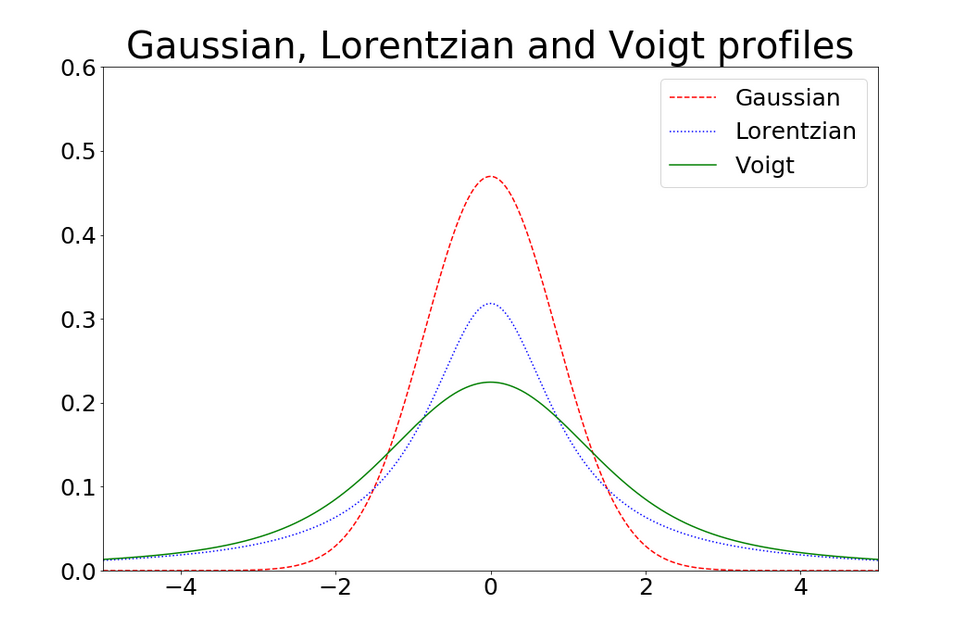
\includegraphics[width=0.5\linewidth]{Figures/1.png}
    \caption{The three profiles}
    \label{fig:enter-label}
\end{figure}
\pagebreak{}
\subsection{Homogeneous and inhomogeneous line broadening}

A transition's spectral profile is considered \textit{homogeneous} if every molecule or atom in state $\ket{i}$ has an equal probability of transitioning to state $\ket{k}$. The probability of emitting radiation is then: 
\begin{equation}
   P(\omega) = A_{ki}g(\omega-\omega_0) 
\end{equation}
Where $A_{ki}$ are the Einstein coefficients of spontaneous emission and $g(\omega-\omega_0)$ is a normalized Lorentzian profile. 

\subsection{Linear absorption spectroscopy} 
Linear absorption spectroscopy is a technique in which an atomic sample (in our case, the rubidium gas), is examined while a tunable single-laser mode laser beam shines at the sample. The frequency of the laser is varied and the intensity pattern of the transmitted beam is measured with a photodiode. 

This method is significantly hindered by the Doppler broadening of absorption lines. For instance, the twelve permissible hyperfine transitions of Rb cannot be individually distinguished using this technique. This is because the Doppler width (approximately 10 GHz) is substantially larger than the frequency gap between the absorption lines, resulting in their overlap. To address this issue, the method of \textit{saturation absorption spectroscopy} is employed.

\subsection{Saturation absorption spectroscopy}

The method of saturation absorption spectroscopy makes it possible to completely eliminate the Doppler background by measuring the difference between the normal and saturated absorption. Thus providing a clear resolution of all the transitions relevant in our experiment. 

In this approach, the beam is divided into two beams with different intensities: a weak probe beam (about 4-5\% of the total intensity) and a pump beam with the rest of the intensity. Both beams strike the gas cell in an opposite direction, and the signal from the probe beam is as a function of the laser frequency.

Consider an atom with two levels and a resonance frequency $\omega_0$. If only the probe beam is used to study the gas cell, we will get the absorption lines we expect to get from linear absorption spectroscopy (with lower intensity). Introducing the pump beam will lead to a very narrow dip in the probe beam signal at the resonance frequency $\omega_0$ (see figure 2). Which can be understood as follows. Atoms with zero velocity component along the z-direction ($v_z = 0$) see both beams as having the same frequency (no Doppler effect). However if an atom happens to have a velocity component along the z-direction, it will see  a shifted frequency of the beams. If the atom is moving to the left (see figure) it will see the probe and pump beams as blue-shifted and red-shifted, respectively. If the atom is moving to the right, the opposite will happen. The pump beam's high intensity will excite all atoms with velocity $v_z = \frac{\omega_L - \omega_0}{\omega_0}c$, where $\omega_L$ is the frequency of the beam. Which will cause absorption for all the atoms with velocity $-v_z$ of the probe beam. Hence, the absorption signal will be the same as in the case of linear absorption spectroscopy. However, if the laser's frequency matches the resonance frequency ($\omega_L = \omega_0$), the atoms with $v_z =0$ will be excited by the high intensity of the pump beam and the ground state will be depleted. Consequently, the absorption rate for the probe beam decreases, leading to a narrow dip with a Lorentzian shape (as the Doppler shift is not present at resonance). This phenomenon is referred to as \textit{hole burning}, and the dips are known as \textit{Lamb dips}.
\begin{figure}[h]
    \centering
    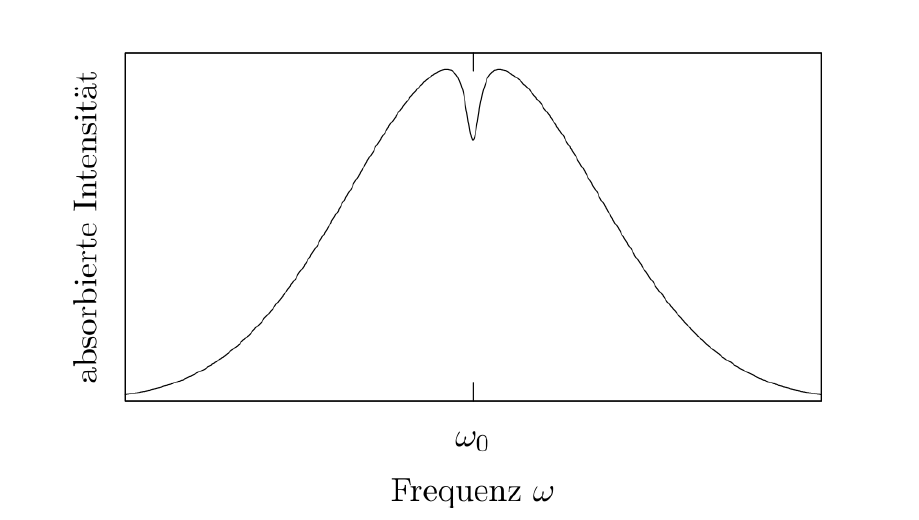
\includegraphics[width=0.5\linewidth]{Figures/3.png}
    \caption{Saturation peak in the Doppler-broadened profile of a two-level atom.}
    \label{fig:enter-label}
\end{figure}
\begin{figure}[h]
    \centering
    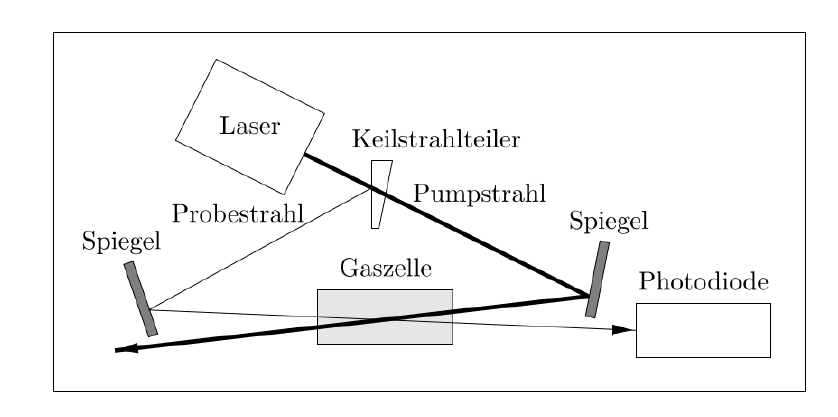
\includegraphics[width=0.5\linewidth]{Figures/2.png}
    \caption{Diagram of the basic setup of saturation absorption spectroscopy.}
    \label{fig:enter-label}
\end{figure}

Now consider a multi-level system. The Doppler broadened absorption lines will have more dips since more transitions can take place and we observe the phenomenon of \textit{cross-over signals}.
Consider a system with three levels, denoted as $N=\{0, 1, 2\}$. If the pump beam’s frequency resonates with either of the transitions $\omega_{01}$ and $\omega_{02}$, two saturation peaks will appear. This is due to the reduction of atoms with a velocity of $v_z = 0$. When the laser frequency is at the average of these frequencies 
\begin{equation}
    \omega_{12} = \frac{\omega_{01}+\omega_{02}}{2}
\end{equation}
the atoms that have a velocity 
\begin{equation}
    v_z = \frac{(\omega_{12}-\omega_{01})c}{\omega_{12}} = \frac{(\omega_{02}-\omega_{01})c}{2\omega_{12}} 
\end{equation}
are excited by the frequency $\omega_{02}$ from the pump beam and the frequency $\omega{01}$ from the probe beam. In a similar fashion, the atoms with velocity 
\begin{equation}
   - v_z = \frac{(\omega_{12}-\omega_{02})c}{\omega_{12}} 
\end{equation}
which gives: 
\begin{equation}
    v_z = \frac{(\omega_{02}-\omega_{01})c}{2\omega_{12}}
\end{equation}
will be excited by the frequency $\omega_{01}$ from the pump beam and the frequency $\omega_{02}$ from the probe beam. Since most atoms are now excited by the pump beam, they are unable to absorb the frequency of the probe beam which manifests as a third dip which is larger than the saturation peaks (Figure 4). This dip is what we call a cross-over peak.

\begin{figure}[h]
    \centering
    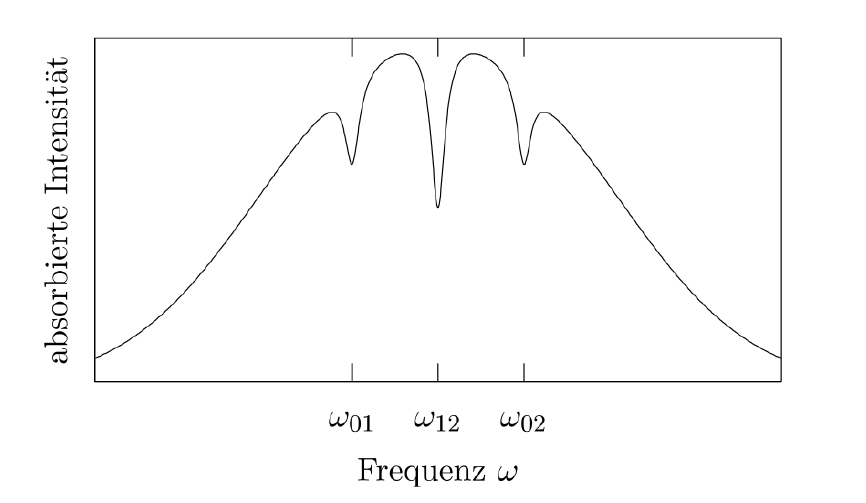
\includegraphics[width=0.5\linewidth]{Figures/4.png}
    \caption{Saturation peaks and crossover signal in the spectrum of a atoms with a three-level systems.}
    \label{fig:enter-label}
\end{figure}

In simpler terms, if two molecular transitions with resonant frequencies $\omega_1$ and $\omega_2$ share a common lower or upper level and overlap within their Doppler width $\delta\omega_D$ (i.e. $|{\omega_1 - \omega_2}| <\delta\omega_D$), a cross-over signal will appear at the frequency $\omega = (\omega_1 + \omega_2)/2$.
\pagebreak{}
\subsection{Fine structure of Rubidium}
Rubidium is an alkali metal that occurs in nature with a mixture of about 72\% $^{85}Rb$ and 28\% $^{87}Rb$. In our experiment, rubidium is present as a gas in a gas cell. This is easily achievable at room temperature since it has a low melting point (around $\SI{39}{\celsius}$) and a boiling point of $\SI{688}{\celsius}$. It is important to note that in alkali metals, all energy levels are filled in the ground state except for the highest one, which is singly occupied. The electron configuration for rubidium in the ground state is $5s^1$. 
\\
Fine structure occurs due to the interaction between electron spin and orbital angular momentum. An extra contribution in the Hamiltonian causes a splitting of the excited states. This contribution is proportional to the product $\vec{S}\cdot\vec{L}$. New quantum numbers are introduced $j$ and $j_z$, which are the eigenvalues of the operator $\vec{J}= \vec{S}+\vec{L}$ and its projection onto the z-axis $\vec{J}_z$ respectively. This is because the operators $\vec{S}$ and $\vec{J}$ don't commute with the Hamiltonian anymore. However, the newly defined total angular momentum $\vec{J}$ does. This definition yields: 
\begin{equation}
    |l-s| \leq j \leq|l+s|
\end{equation}
In spectroscopic notation, the ground state of rubidium is $5^2S_{3/2}$ (i.e. $l=0$,$s=1/2$,$j = 1/2$). The splitting of the first excited state of rubidium is interpreted as having two values of $j$ which are $j =1/2$ and $j =3/2$, resulting in the two states $5^2P_{1/2}$ and $5^2P_{3/2}$, respectively. Hence, two different transitions can take place, termed the $D_1$ and $D_2$ lines: 
\begin{equation}
    \begin{aligned}
& D_1: 5^2 S_{\frac{1}{2}} \Rightarrow 5^2 P_{\frac{1}{2}} \nu_{1}=\SI{377.1}{THz} \\
& D_2: 5^2 S_{\frac{1}{2}} \Rightarrow 5^2 P_{\frac{3}{2}} \nu_{2}=\SI{384.2}{THz} 
\end{aligned}
\end{equation}
In our experiment, we work with the $D_2$ line. 
\pagebreak{}
\subsection{Hyperfine structure of Rubidium}

Since nuclei are made of neutrons and protons, they have an intrinsic angular momentum $\vec{I}$. The interaction between $\vec{I}$ and $\vec{J}$ leads to further splitting in the same spirit as spin-orbit coupling. A new operator is defined as $\vec{F} = \vec{I}+\vec{J}$ with an eigenvalue $f$ taking the values $|j-i| \leq f \leq|j+i|$. The interaction strength and hence the splitting will be different between the two isotopes of rubidium that we are working with. The energy levels that result from the splitting are: 
\begin{equation}
    \begin{gathered}
\text { ground state: } \\
{ }^{85} R b: j=\frac{1}{2} \Rightarrow i=\frac{3}{2}, f=1,2 \\
{ }^{87} R b: j=\frac{1}{2} \Rightarrow i=\frac{5}{2}, f=2,3 \\
\text { excited state: } \\
{ }^{85} R b: j=\frac{1}{2} \Rightarrow i=\frac{3}{2}, f=1,2 \\
{ }^{85} R b: j=\frac{3}{2} \Rightarrow i=\frac{3}{2}, f=0,3 \\
{ }^{87} R b: j=\frac{1}{2} \Rightarrow i=\frac{5}{2}, f=2,3 \\
{ }^{87} R b: j=\frac{3}{2} \Rightarrow i=\frac{5}{2}, f=1,4
\end{gathered}
\end{equation}

\subsection{Semiconductor basics}
Semiconductors are solids that have a conductivity between that of a conductor and an insulator. Their energy levels sit close to each other in what is known as 'band structure'. The lower energy band is known as the valence band while the higher energy one is the conduction band. There is an energy gap (the \textit{band gap)} between the two bands where no energy level is allowed. At the middle of the band gap lays the Fermi level, which at absolute zero, separates the fully empty conduction band from the fully occupied valence band. The position of the Fermi level affects the conductivity of the semiconductor, and it can be controlled with the method of \textit{doping}.
\begin{figure}[h]
    \centering
    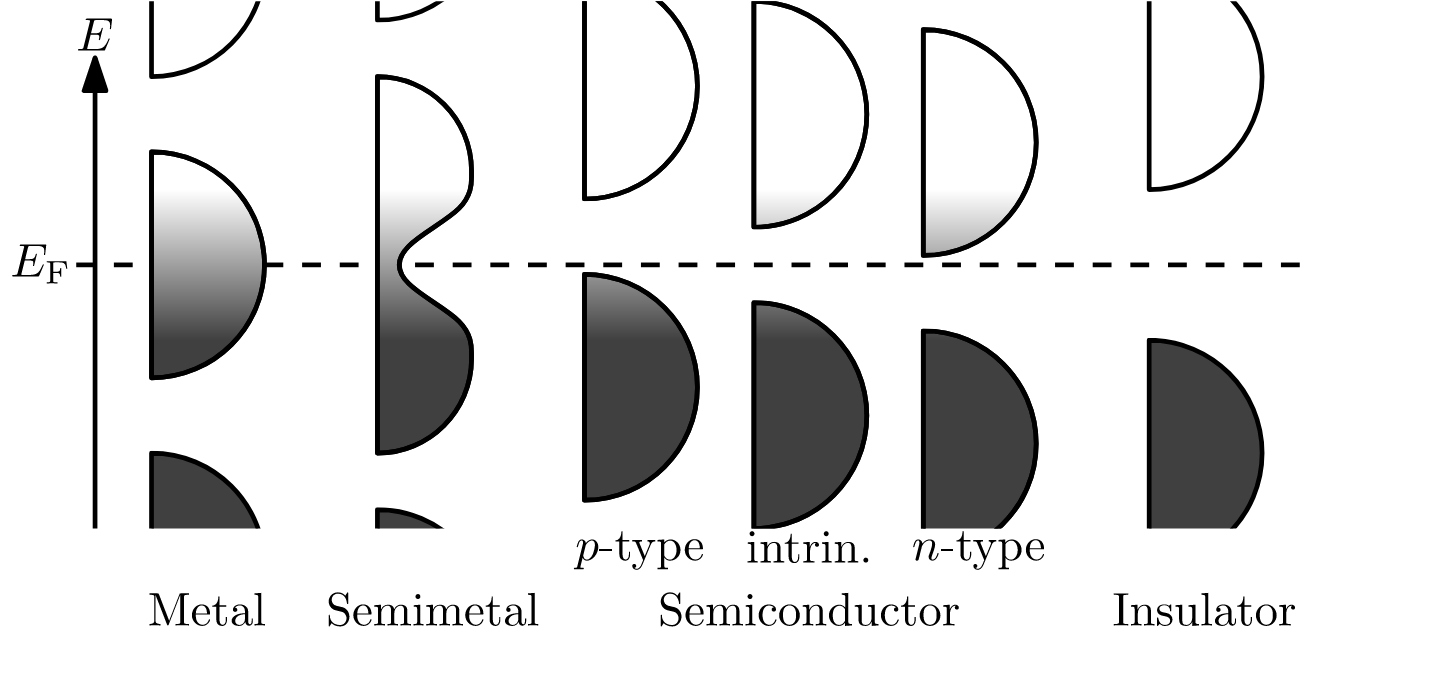
\includegraphics[width=0.5\linewidth]{Figures/wiki2.png}
    \caption{Position of Fermi level in different materials \cite{wikipediacontributors_2019_semiconductor}}
    \label{fig:enter-label}
\end{figure}


\subsection{Doping}
Doping is a technique that involves substituting a semiconductor lattice atom with another atom that has a different number of valence electrons. There are two kind of doping, n-doping and p-doping. P-doping involves replacing an atom from the lattice by another atom that has fewer valence electrons. In n-doping the impurity has more valence electrons than the lattice atoms. P-doping introduces a 'hole', which is an absence of an electron and is equivalent to a positive charge. Doping is useful because it lets us modify the conductivity of a semi-conductor. For example, in n-doping, the Fermi level is shifted and becomes closer to the conduction band, making it possible for an electron to jump to the conduction band via thermal excitations. This leads to an increase in the density of free charge carriers and hence the conductivity of the lattice. 
\begin{figure}[h]
    \centering
    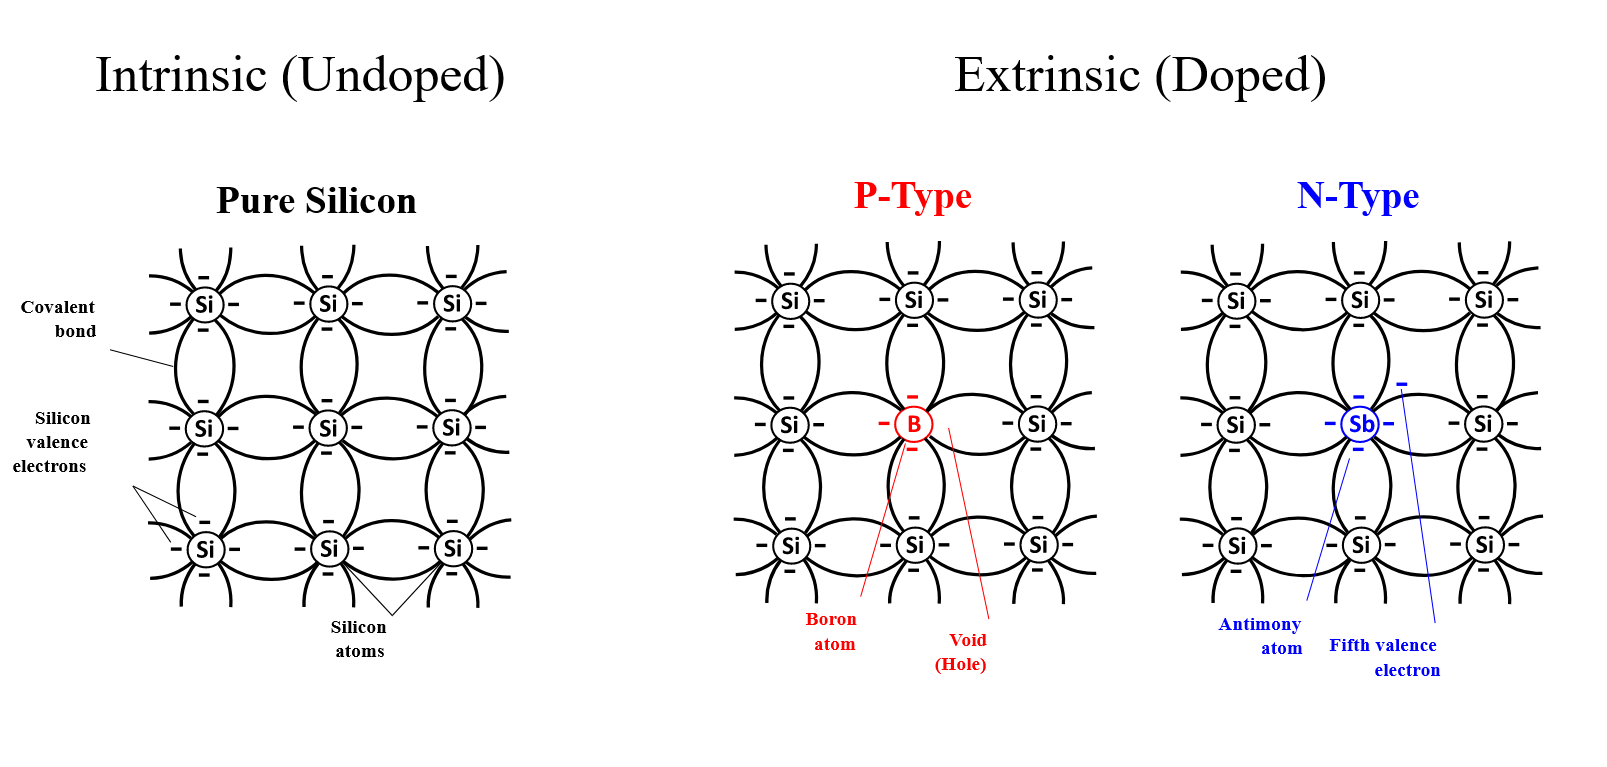
\includegraphics[width=0.5\linewidth]{Figures/wiki1.png}
    \caption{Doping of a pure silicon array. Silicon based intrinsic semiconductor becomes extrinsic when impurities such as Boron and Antimony are introduced. \cite{wikipediacontributors_2019_doping}}
    \label{fig:enter-label}
\end{figure}
\pagebreak{}
\subsection{The p-n junction}
A p-n junction is a combination of a p- and n- doped semiconductors. When the two regions come in contact, a recombination of the charges happens. At the junction, some free electrons in the n-type region migrate into the p-type region due to random thermal motion. As these electrons diffuse into the p-type, they combine with holes, neutralizing each other. Similarly, some positive holes in the p-type diffuse into the n-type, where they combine with free electrons, also neutralizing each other. The positively charged ("donor") dopant atoms in the n-type region are fixed within the crystal lattice and cannot move, resulting in a region near the junction with a fixed positive charge. Conversely, the negatively charged ("acceptor") dopant atoms in the p-type region are also fixed, leading to a region near the junction with a fixed negative charge. This creates an electric field that repels mobile charges away from the junction, causing the regions near the p-n interface to lose their neutrality and lose most of their mobile carriers. This electric field prohibits any further diffusion from taking place. With sufficiently strong doping, the Fermi level of the p-region will shift into the valence band, while the Fermi level of the n-region will shift into the conduction band. 

\subsection{Effect of external voltage}
When an external voltage is applied, a p-n junction forms a diode, which allows current to flow in one direction while blocking it in the opposite direction. If the voltage creates a 'forward bias,' charges move through the diode and continue into the circuit. Conversely, if the voltage creates a 'reverse bias,' the charges promote recombination, expanding the charge-carrier-free region and increasing the potential barrier.

\subsection{Laser diode}
A laser is a light source that emits very coherent and monochromatic light. The operation of a laser relies on stimulated emission, a process where a radiation field excites electron-hole pairs using photons of the appropriate wavelength. This excitation results in the recombining quasiparticle pair emitting radiation that matches the wavelength, phase, and direction of the incoming photon, effectively creating a "copy" of the original photon. Since spontaneous and stimulated emission always occur simultaneously, stimulated emission must dominate for lasing to occur. To achieve this, a laser diode is constructed as an optical resonator, which is a region bounded by two highly reflective mirrors with a length precisely tailored to the emission wavelength of the material. Emitted photons could be immediately absorbed, preventing the progressive 'multiplication' of photons. Therefore, we need the 'gain'—the difference between spontaneous emission and absorption—to be as large as possible. To achieve a positive gain, population inversion is necessary: the number of electrons in the conduction band must significantly exceed the number in the corresponding valence band.

\pagebreak{}
\subsection{Fabry Perot Interferometer}

The Fabry-Pérot interferometer (FPI) selectively transmits signals based on their wavelength. It consists of two highly reflective parallel surfaces separated by a distance \(d\). For an electromagnetic wave with frequency \(\nu\) and wavenumber \(k = \frac{2\pi\nu}{c}\), the wave equation is expressed as:

\[
\phi(r, t) = U(r)\exp(i\omega t)
\]

This wave must satisfy the Helmholtz equation and vanish at the edges of the interferometer, a condition met only by resonant modes corresponding to resonant frequencies:

\[
\frac{d}{\lambda_n} = 2n \quad \Rightarrow \quad k_n = \frac{2\pi}{\lambda_n} \quad \Rightarrow \quad k_n \cdot n = \frac{\pi n}{d}
\]

This results in:

\[
\nu_n = \frac{c}{\lambda_n} = \frac{nc}{2d}
\]

The spacing between adjacent resonant frequency modes, known as the Free Spectral Range (FSR), is:

\[
\text{FSR} = \frac{(n+1-n)c}{2d} = \frac{c}{2d}
\]

Upon entering the FPI, the wave is reflected multiple times, with its amplitude decreasing by the reflectivity factor \(r\) with each reflection. The phase difference between the original and reflected waves is \(\phi = 2dk\), as the wave travels the distance \(d\) twice before returning to the incidence point.

By summing the amplitudes of the interfering waves using a geometric series, the intensity (the square of the sum of the amplitudes) is given by:

\[
I = \frac{I_0}{(1-r)^2 + 4r \sin^2\left(\frac{\phi}{2}\right)} = \frac{I_{\text{max}}}{1 + \left(\frac{2F}{\pi}\right)^2 \sin^2\left(\frac{\phi}{2}\right)}
\]

Here, \(F\) represents the interferometer's finesse:

\[
F = \frac{\pi\sqrt{r}}{1-r} = \frac{\pi}{T + L}
\]

The maximum intensity is \(I_{\text{max}} = \frac{I_0}{(1-r)^2}\). Finally, with the FSR denoted as \(\nu_F\), the full width at half maximum (FWHM) of the intensity profile can be expressed as:


\begin{equation}
	\delta \nu = \frac{\nu_{\text{FSR}}}{\mathscr{F}}
	\label{eq:finesse}
\end{equation}

\pagebreak{}

\section{Analysis}

\subsection{Task 1}

We were instructed to scale our measurement data using the FPI peaks in addition to determining the finesse.

\subsubsection{Scaling the data}

From \cite{jung_2018_dopplerfree}, we know that our FSR is $1$ GHz. Therefore, if the average spacing between peaks is calculated, we can determine the conversion factor and scale our data accordingly.

\begin{figure}[h]
	\centering
	\begin{subfigure}[t]{0.45\textwidth}
		\centering
		\scalebox{0.5}{%% Creator: Matplotlib, PGF backend
%%
%% To include the figure in your LaTeX document, write
%%   \input{<filename>.pgf}
%%
%% Make sure the required packages are loaded in your preamble
%%   \usepackage{pgf}
%%
%% Also ensure that all the required font packages are loaded; for instance,
%% the lmodern package is sometimes necessary when using math font.
%%   \usepackage{lmodern}
%%
%% Figures using additional raster images can only be included by \input if
%% they are in the same directory as the main LaTeX file. For loading figures
%% from other directories you can use the `import` package
%%   \usepackage{import}
%%
%% and then include the figures with
%%   \import{<path to file>}{<filename>.pgf}
%%
%% Matplotlib used the following preamble
%%   
%%   \usepackage{fontspec}
%%   \makeatletter\@ifpackageloaded{underscore}{}{\usepackage[strings]{underscore}}\makeatother
%%
\begingroup%
\makeatletter%
\begin{pgfpicture}%
\pgfpathrectangle{\pgfpointorigin}{\pgfqpoint{6.489553in}{4.010764in}}%
\pgfusepath{use as bounding box, clip}%
\begin{pgfscope}%
\pgfsetbuttcap%
\pgfsetmiterjoin%
\definecolor{currentfill}{rgb}{1.000000,1.000000,1.000000}%
\pgfsetfillcolor{currentfill}%
\pgfsetlinewidth{0.000000pt}%
\definecolor{currentstroke}{rgb}{1.000000,1.000000,1.000000}%
\pgfsetstrokecolor{currentstroke}%
\pgfsetdash{}{0pt}%
\pgfpathmoveto{\pgfqpoint{0.000000in}{0.000000in}}%
\pgfpathlineto{\pgfqpoint{6.489553in}{0.000000in}}%
\pgfpathlineto{\pgfqpoint{6.489553in}{4.010764in}}%
\pgfpathlineto{\pgfqpoint{0.000000in}{4.010764in}}%
\pgfpathlineto{\pgfqpoint{0.000000in}{0.000000in}}%
\pgfpathclose%
\pgfusepath{fill}%
\end{pgfscope}%
\begin{pgfscope}%
\pgfsetbuttcap%
\pgfsetmiterjoin%
\definecolor{currentfill}{rgb}{1.000000,1.000000,1.000000}%
\pgfsetfillcolor{currentfill}%
\pgfsetlinewidth{0.000000pt}%
\definecolor{currentstroke}{rgb}{0.000000,0.000000,0.000000}%
\pgfsetstrokecolor{currentstroke}%
\pgfsetstrokeopacity{0.000000}%
\pgfsetdash{}{0pt}%
\pgfpathmoveto{\pgfqpoint{0.811194in}{0.441184in}}%
\pgfpathlineto{\pgfqpoint{5.840598in}{0.441184in}}%
\pgfpathlineto{\pgfqpoint{5.840598in}{3.529473in}}%
\pgfpathlineto{\pgfqpoint{0.811194in}{3.529473in}}%
\pgfpathlineto{\pgfqpoint{0.811194in}{0.441184in}}%
\pgfpathclose%
\pgfusepath{fill}%
\end{pgfscope}%
\begin{pgfscope}%
\pgfsetbuttcap%
\pgfsetroundjoin%
\definecolor{currentfill}{rgb}{0.000000,0.000000,0.000000}%
\pgfsetfillcolor{currentfill}%
\pgfsetlinewidth{0.803000pt}%
\definecolor{currentstroke}{rgb}{0.000000,0.000000,0.000000}%
\pgfsetstrokecolor{currentstroke}%
\pgfsetdash{}{0pt}%
\pgfsys@defobject{currentmarker}{\pgfqpoint{0.000000in}{-0.048611in}}{\pgfqpoint{0.000000in}{0.000000in}}{%
\pgfpathmoveto{\pgfqpoint{0.000000in}{0.000000in}}%
\pgfpathlineto{\pgfqpoint{0.000000in}{-0.048611in}}%
\pgfusepath{stroke,fill}%
}%
\begin{pgfscope}%
\pgfsys@transformshift{0.893643in}{0.441184in}%
\pgfsys@useobject{currentmarker}{}%
\end{pgfscope}%
\end{pgfscope}%
\begin{pgfscope}%
\definecolor{textcolor}{rgb}{0.000000,0.000000,0.000000}%
\pgfsetstrokecolor{textcolor}%
\pgfsetfillcolor{textcolor}%
\pgftext[x=0.893643in,y=0.343962in,,top]{\color{textcolor}\rmfamily\fontsize{10.000000}{12.000000}\selectfont \(\displaystyle {0}\)}%
\end{pgfscope}%
\begin{pgfscope}%
\pgfsetbuttcap%
\pgfsetroundjoin%
\definecolor{currentfill}{rgb}{0.000000,0.000000,0.000000}%
\pgfsetfillcolor{currentfill}%
\pgfsetlinewidth{0.803000pt}%
\definecolor{currentstroke}{rgb}{0.000000,0.000000,0.000000}%
\pgfsetstrokecolor{currentstroke}%
\pgfsetdash{}{0pt}%
\pgfsys@defobject{currentmarker}{\pgfqpoint{0.000000in}{-0.048611in}}{\pgfqpoint{0.000000in}{0.000000in}}{%
\pgfpathmoveto{\pgfqpoint{0.000000in}{0.000000in}}%
\pgfpathlineto{\pgfqpoint{0.000000in}{-0.048611in}}%
\pgfusepath{stroke,fill}%
}%
\begin{pgfscope}%
\pgfsys@transformshift{1.718136in}{0.441184in}%
\pgfsys@useobject{currentmarker}{}%
\end{pgfscope}%
\end{pgfscope}%
\begin{pgfscope}%
\definecolor{textcolor}{rgb}{0.000000,0.000000,0.000000}%
\pgfsetstrokecolor{textcolor}%
\pgfsetfillcolor{textcolor}%
\pgftext[x=1.718136in,y=0.343962in,,top]{\color{textcolor}\rmfamily\fontsize{10.000000}{12.000000}\selectfont \(\displaystyle {100}\)}%
\end{pgfscope}%
\begin{pgfscope}%
\pgfsetbuttcap%
\pgfsetroundjoin%
\definecolor{currentfill}{rgb}{0.000000,0.000000,0.000000}%
\pgfsetfillcolor{currentfill}%
\pgfsetlinewidth{0.803000pt}%
\definecolor{currentstroke}{rgb}{0.000000,0.000000,0.000000}%
\pgfsetstrokecolor{currentstroke}%
\pgfsetdash{}{0pt}%
\pgfsys@defobject{currentmarker}{\pgfqpoint{0.000000in}{-0.048611in}}{\pgfqpoint{0.000000in}{0.000000in}}{%
\pgfpathmoveto{\pgfqpoint{0.000000in}{0.000000in}}%
\pgfpathlineto{\pgfqpoint{0.000000in}{-0.048611in}}%
\pgfusepath{stroke,fill}%
}%
\begin{pgfscope}%
\pgfsys@transformshift{2.542628in}{0.441184in}%
\pgfsys@useobject{currentmarker}{}%
\end{pgfscope}%
\end{pgfscope}%
\begin{pgfscope}%
\definecolor{textcolor}{rgb}{0.000000,0.000000,0.000000}%
\pgfsetstrokecolor{textcolor}%
\pgfsetfillcolor{textcolor}%
\pgftext[x=2.542628in,y=0.343962in,,top]{\color{textcolor}\rmfamily\fontsize{10.000000}{12.000000}\selectfont \(\displaystyle {200}\)}%
\end{pgfscope}%
\begin{pgfscope}%
\pgfsetbuttcap%
\pgfsetroundjoin%
\definecolor{currentfill}{rgb}{0.000000,0.000000,0.000000}%
\pgfsetfillcolor{currentfill}%
\pgfsetlinewidth{0.803000pt}%
\definecolor{currentstroke}{rgb}{0.000000,0.000000,0.000000}%
\pgfsetstrokecolor{currentstroke}%
\pgfsetdash{}{0pt}%
\pgfsys@defobject{currentmarker}{\pgfqpoint{0.000000in}{-0.048611in}}{\pgfqpoint{0.000000in}{0.000000in}}{%
\pgfpathmoveto{\pgfqpoint{0.000000in}{0.000000in}}%
\pgfpathlineto{\pgfqpoint{0.000000in}{-0.048611in}}%
\pgfusepath{stroke,fill}%
}%
\begin{pgfscope}%
\pgfsys@transformshift{3.367121in}{0.441184in}%
\pgfsys@useobject{currentmarker}{}%
\end{pgfscope}%
\end{pgfscope}%
\begin{pgfscope}%
\definecolor{textcolor}{rgb}{0.000000,0.000000,0.000000}%
\pgfsetstrokecolor{textcolor}%
\pgfsetfillcolor{textcolor}%
\pgftext[x=3.367121in,y=0.343962in,,top]{\color{textcolor}\rmfamily\fontsize{10.000000}{12.000000}\selectfont \(\displaystyle {300}\)}%
\end{pgfscope}%
\begin{pgfscope}%
\pgfsetbuttcap%
\pgfsetroundjoin%
\definecolor{currentfill}{rgb}{0.000000,0.000000,0.000000}%
\pgfsetfillcolor{currentfill}%
\pgfsetlinewidth{0.803000pt}%
\definecolor{currentstroke}{rgb}{0.000000,0.000000,0.000000}%
\pgfsetstrokecolor{currentstroke}%
\pgfsetdash{}{0pt}%
\pgfsys@defobject{currentmarker}{\pgfqpoint{0.000000in}{-0.048611in}}{\pgfqpoint{0.000000in}{0.000000in}}{%
\pgfpathmoveto{\pgfqpoint{0.000000in}{0.000000in}}%
\pgfpathlineto{\pgfqpoint{0.000000in}{-0.048611in}}%
\pgfusepath{stroke,fill}%
}%
\begin{pgfscope}%
\pgfsys@transformshift{4.191613in}{0.441184in}%
\pgfsys@useobject{currentmarker}{}%
\end{pgfscope}%
\end{pgfscope}%
\begin{pgfscope}%
\definecolor{textcolor}{rgb}{0.000000,0.000000,0.000000}%
\pgfsetstrokecolor{textcolor}%
\pgfsetfillcolor{textcolor}%
\pgftext[x=4.191613in,y=0.343962in,,top]{\color{textcolor}\rmfamily\fontsize{10.000000}{12.000000}\selectfont \(\displaystyle {400}\)}%
\end{pgfscope}%
\begin{pgfscope}%
\pgfsetbuttcap%
\pgfsetroundjoin%
\definecolor{currentfill}{rgb}{0.000000,0.000000,0.000000}%
\pgfsetfillcolor{currentfill}%
\pgfsetlinewidth{0.803000pt}%
\definecolor{currentstroke}{rgb}{0.000000,0.000000,0.000000}%
\pgfsetstrokecolor{currentstroke}%
\pgfsetdash{}{0pt}%
\pgfsys@defobject{currentmarker}{\pgfqpoint{0.000000in}{-0.048611in}}{\pgfqpoint{0.000000in}{0.000000in}}{%
\pgfpathmoveto{\pgfqpoint{0.000000in}{0.000000in}}%
\pgfpathlineto{\pgfqpoint{0.000000in}{-0.048611in}}%
\pgfusepath{stroke,fill}%
}%
\begin{pgfscope}%
\pgfsys@transformshift{5.016105in}{0.441184in}%
\pgfsys@useobject{currentmarker}{}%
\end{pgfscope}%
\end{pgfscope}%
\begin{pgfscope}%
\definecolor{textcolor}{rgb}{0.000000,0.000000,0.000000}%
\pgfsetstrokecolor{textcolor}%
\pgfsetfillcolor{textcolor}%
\pgftext[x=5.016105in,y=0.343962in,,top]{\color{textcolor}\rmfamily\fontsize{10.000000}{12.000000}\selectfont \(\displaystyle {500}\)}%
\end{pgfscope}%
\begin{pgfscope}%
\pgfsetbuttcap%
\pgfsetroundjoin%
\definecolor{currentfill}{rgb}{0.000000,0.000000,0.000000}%
\pgfsetfillcolor{currentfill}%
\pgfsetlinewidth{0.803000pt}%
\definecolor{currentstroke}{rgb}{0.000000,0.000000,0.000000}%
\pgfsetstrokecolor{currentstroke}%
\pgfsetdash{}{0pt}%
\pgfsys@defobject{currentmarker}{\pgfqpoint{0.000000in}{-0.048611in}}{\pgfqpoint{0.000000in}{0.000000in}}{%
\pgfpathmoveto{\pgfqpoint{0.000000in}{0.000000in}}%
\pgfpathlineto{\pgfqpoint{0.000000in}{-0.048611in}}%
\pgfusepath{stroke,fill}%
}%
\begin{pgfscope}%
\pgfsys@transformshift{5.840598in}{0.441184in}%
\pgfsys@useobject{currentmarker}{}%
\end{pgfscope}%
\end{pgfscope}%
\begin{pgfscope}%
\definecolor{textcolor}{rgb}{0.000000,0.000000,0.000000}%
\pgfsetstrokecolor{textcolor}%
\pgfsetfillcolor{textcolor}%
\pgftext[x=5.840598in,y=0.343962in,,top]{\color{textcolor}\rmfamily\fontsize{10.000000}{12.000000}\selectfont \(\displaystyle {600}\)}%
\end{pgfscope}%
\begin{pgfscope}%
\definecolor{textcolor}{rgb}{0.000000,0.000000,0.000000}%
\pgfsetstrokecolor{textcolor}%
\pgfsetfillcolor{textcolor}%
\pgftext[x=3.325896in,y=0.165073in,,top]{\color{textcolor}\rmfamily\fontsize{10.000000}{12.000000}\selectfont Counts [a.u.]}%
\end{pgfscope}%
\begin{pgfscope}%
\pgfsetbuttcap%
\pgfsetroundjoin%
\definecolor{currentfill}{rgb}{0.000000,0.000000,0.000000}%
\pgfsetfillcolor{currentfill}%
\pgfsetlinewidth{0.803000pt}%
\definecolor{currentstroke}{rgb}{0.000000,0.000000,0.000000}%
\pgfsetstrokecolor{currentstroke}%
\pgfsetdash{}{0pt}%
\pgfsys@defobject{currentmarker}{\pgfqpoint{-0.048611in}{0.000000in}}{\pgfqpoint{-0.000000in}{0.000000in}}{%
\pgfpathmoveto{\pgfqpoint{-0.000000in}{0.000000in}}%
\pgfpathlineto{\pgfqpoint{-0.048611in}{0.000000in}}%
\pgfusepath{stroke,fill}%
}%
\begin{pgfscope}%
\pgfsys@transformshift{0.811194in}{0.493274in}%
\pgfsys@useobject{currentmarker}{}%
\end{pgfscope}%
\end{pgfscope}%
\begin{pgfscope}%
\definecolor{textcolor}{rgb}{0.000000,0.000000,0.000000}%
\pgfsetstrokecolor{textcolor}%
\pgfsetfillcolor{textcolor}%
\pgftext[x=0.428477in, y=0.445079in, left, base]{\color{textcolor}\rmfamily\fontsize{10.000000}{12.000000}\selectfont \(\displaystyle {\ensuremath{-}1.6}\)}%
\end{pgfscope}%
\begin{pgfscope}%
\pgfsetbuttcap%
\pgfsetroundjoin%
\definecolor{currentfill}{rgb}{0.000000,0.000000,0.000000}%
\pgfsetfillcolor{currentfill}%
\pgfsetlinewidth{0.803000pt}%
\definecolor{currentstroke}{rgb}{0.000000,0.000000,0.000000}%
\pgfsetstrokecolor{currentstroke}%
\pgfsetdash{}{0pt}%
\pgfsys@defobject{currentmarker}{\pgfqpoint{-0.048611in}{0.000000in}}{\pgfqpoint{-0.000000in}{0.000000in}}{%
\pgfpathmoveto{\pgfqpoint{-0.000000in}{0.000000in}}%
\pgfpathlineto{\pgfqpoint{-0.048611in}{0.000000in}}%
\pgfusepath{stroke,fill}%
}%
\begin{pgfscope}%
\pgfsys@transformshift{0.811194in}{0.846423in}%
\pgfsys@useobject{currentmarker}{}%
\end{pgfscope}%
\end{pgfscope}%
\begin{pgfscope}%
\definecolor{textcolor}{rgb}{0.000000,0.000000,0.000000}%
\pgfsetstrokecolor{textcolor}%
\pgfsetfillcolor{textcolor}%
\pgftext[x=0.428477in, y=0.798228in, left, base]{\color{textcolor}\rmfamily\fontsize{10.000000}{12.000000}\selectfont \(\displaystyle {\ensuremath{-}1.4}\)}%
\end{pgfscope}%
\begin{pgfscope}%
\pgfsetbuttcap%
\pgfsetroundjoin%
\definecolor{currentfill}{rgb}{0.000000,0.000000,0.000000}%
\pgfsetfillcolor{currentfill}%
\pgfsetlinewidth{0.803000pt}%
\definecolor{currentstroke}{rgb}{0.000000,0.000000,0.000000}%
\pgfsetstrokecolor{currentstroke}%
\pgfsetdash{}{0pt}%
\pgfsys@defobject{currentmarker}{\pgfqpoint{-0.048611in}{0.000000in}}{\pgfqpoint{-0.000000in}{0.000000in}}{%
\pgfpathmoveto{\pgfqpoint{-0.000000in}{0.000000in}}%
\pgfpathlineto{\pgfqpoint{-0.048611in}{0.000000in}}%
\pgfusepath{stroke,fill}%
}%
\begin{pgfscope}%
\pgfsys@transformshift{0.811194in}{1.199572in}%
\pgfsys@useobject{currentmarker}{}%
\end{pgfscope}%
\end{pgfscope}%
\begin{pgfscope}%
\definecolor{textcolor}{rgb}{0.000000,0.000000,0.000000}%
\pgfsetstrokecolor{textcolor}%
\pgfsetfillcolor{textcolor}%
\pgftext[x=0.428477in, y=1.151377in, left, base]{\color{textcolor}\rmfamily\fontsize{10.000000}{12.000000}\selectfont \(\displaystyle {\ensuremath{-}1.2}\)}%
\end{pgfscope}%
\begin{pgfscope}%
\pgfsetbuttcap%
\pgfsetroundjoin%
\definecolor{currentfill}{rgb}{0.000000,0.000000,0.000000}%
\pgfsetfillcolor{currentfill}%
\pgfsetlinewidth{0.803000pt}%
\definecolor{currentstroke}{rgb}{0.000000,0.000000,0.000000}%
\pgfsetstrokecolor{currentstroke}%
\pgfsetdash{}{0pt}%
\pgfsys@defobject{currentmarker}{\pgfqpoint{-0.048611in}{0.000000in}}{\pgfqpoint{-0.000000in}{0.000000in}}{%
\pgfpathmoveto{\pgfqpoint{-0.000000in}{0.000000in}}%
\pgfpathlineto{\pgfqpoint{-0.048611in}{0.000000in}}%
\pgfusepath{stroke,fill}%
}%
\begin{pgfscope}%
\pgfsys@transformshift{0.811194in}{1.552721in}%
\pgfsys@useobject{currentmarker}{}%
\end{pgfscope}%
\end{pgfscope}%
\begin{pgfscope}%
\definecolor{textcolor}{rgb}{0.000000,0.000000,0.000000}%
\pgfsetstrokecolor{textcolor}%
\pgfsetfillcolor{textcolor}%
\pgftext[x=0.428477in, y=1.504526in, left, base]{\color{textcolor}\rmfamily\fontsize{10.000000}{12.000000}\selectfont \(\displaystyle {\ensuremath{-}1.0}\)}%
\end{pgfscope}%
\begin{pgfscope}%
\pgfsetbuttcap%
\pgfsetroundjoin%
\definecolor{currentfill}{rgb}{0.000000,0.000000,0.000000}%
\pgfsetfillcolor{currentfill}%
\pgfsetlinewidth{0.803000pt}%
\definecolor{currentstroke}{rgb}{0.000000,0.000000,0.000000}%
\pgfsetstrokecolor{currentstroke}%
\pgfsetdash{}{0pt}%
\pgfsys@defobject{currentmarker}{\pgfqpoint{-0.048611in}{0.000000in}}{\pgfqpoint{-0.000000in}{0.000000in}}{%
\pgfpathmoveto{\pgfqpoint{-0.000000in}{0.000000in}}%
\pgfpathlineto{\pgfqpoint{-0.048611in}{0.000000in}}%
\pgfusepath{stroke,fill}%
}%
\begin{pgfscope}%
\pgfsys@transformshift{0.811194in}{1.905870in}%
\pgfsys@useobject{currentmarker}{}%
\end{pgfscope}%
\end{pgfscope}%
\begin{pgfscope}%
\definecolor{textcolor}{rgb}{0.000000,0.000000,0.000000}%
\pgfsetstrokecolor{textcolor}%
\pgfsetfillcolor{textcolor}%
\pgftext[x=0.428477in, y=1.857675in, left, base]{\color{textcolor}\rmfamily\fontsize{10.000000}{12.000000}\selectfont \(\displaystyle {\ensuremath{-}0.8}\)}%
\end{pgfscope}%
\begin{pgfscope}%
\pgfsetbuttcap%
\pgfsetroundjoin%
\definecolor{currentfill}{rgb}{0.000000,0.000000,0.000000}%
\pgfsetfillcolor{currentfill}%
\pgfsetlinewidth{0.803000pt}%
\definecolor{currentstroke}{rgb}{0.000000,0.000000,0.000000}%
\pgfsetstrokecolor{currentstroke}%
\pgfsetdash{}{0pt}%
\pgfsys@defobject{currentmarker}{\pgfqpoint{-0.048611in}{0.000000in}}{\pgfqpoint{-0.000000in}{0.000000in}}{%
\pgfpathmoveto{\pgfqpoint{-0.000000in}{0.000000in}}%
\pgfpathlineto{\pgfqpoint{-0.048611in}{0.000000in}}%
\pgfusepath{stroke,fill}%
}%
\begin{pgfscope}%
\pgfsys@transformshift{0.811194in}{2.259019in}%
\pgfsys@useobject{currentmarker}{}%
\end{pgfscope}%
\end{pgfscope}%
\begin{pgfscope}%
\definecolor{textcolor}{rgb}{0.000000,0.000000,0.000000}%
\pgfsetstrokecolor{textcolor}%
\pgfsetfillcolor{textcolor}%
\pgftext[x=0.428477in, y=2.210824in, left, base]{\color{textcolor}\rmfamily\fontsize{10.000000}{12.000000}\selectfont \(\displaystyle {\ensuremath{-}0.6}\)}%
\end{pgfscope}%
\begin{pgfscope}%
\pgfsetbuttcap%
\pgfsetroundjoin%
\definecolor{currentfill}{rgb}{0.000000,0.000000,0.000000}%
\pgfsetfillcolor{currentfill}%
\pgfsetlinewidth{0.803000pt}%
\definecolor{currentstroke}{rgb}{0.000000,0.000000,0.000000}%
\pgfsetstrokecolor{currentstroke}%
\pgfsetdash{}{0pt}%
\pgfsys@defobject{currentmarker}{\pgfqpoint{-0.048611in}{0.000000in}}{\pgfqpoint{-0.000000in}{0.000000in}}{%
\pgfpathmoveto{\pgfqpoint{-0.000000in}{0.000000in}}%
\pgfpathlineto{\pgfqpoint{-0.048611in}{0.000000in}}%
\pgfusepath{stroke,fill}%
}%
\begin{pgfscope}%
\pgfsys@transformshift{0.811194in}{2.612168in}%
\pgfsys@useobject{currentmarker}{}%
\end{pgfscope}%
\end{pgfscope}%
\begin{pgfscope}%
\definecolor{textcolor}{rgb}{0.000000,0.000000,0.000000}%
\pgfsetstrokecolor{textcolor}%
\pgfsetfillcolor{textcolor}%
\pgftext[x=0.428477in, y=2.563974in, left, base]{\color{textcolor}\rmfamily\fontsize{10.000000}{12.000000}\selectfont \(\displaystyle {\ensuremath{-}0.4}\)}%
\end{pgfscope}%
\begin{pgfscope}%
\pgfsetbuttcap%
\pgfsetroundjoin%
\definecolor{currentfill}{rgb}{0.000000,0.000000,0.000000}%
\pgfsetfillcolor{currentfill}%
\pgfsetlinewidth{0.803000pt}%
\definecolor{currentstroke}{rgb}{0.000000,0.000000,0.000000}%
\pgfsetstrokecolor{currentstroke}%
\pgfsetdash{}{0pt}%
\pgfsys@defobject{currentmarker}{\pgfqpoint{-0.048611in}{0.000000in}}{\pgfqpoint{-0.000000in}{0.000000in}}{%
\pgfpathmoveto{\pgfqpoint{-0.000000in}{0.000000in}}%
\pgfpathlineto{\pgfqpoint{-0.048611in}{0.000000in}}%
\pgfusepath{stroke,fill}%
}%
\begin{pgfscope}%
\pgfsys@transformshift{0.811194in}{2.965317in}%
\pgfsys@useobject{currentmarker}{}%
\end{pgfscope}%
\end{pgfscope}%
\begin{pgfscope}%
\definecolor{textcolor}{rgb}{0.000000,0.000000,0.000000}%
\pgfsetstrokecolor{textcolor}%
\pgfsetfillcolor{textcolor}%
\pgftext[x=0.428477in, y=2.917123in, left, base]{\color{textcolor}\rmfamily\fontsize{10.000000}{12.000000}\selectfont \(\displaystyle {\ensuremath{-}0.2}\)}%
\end{pgfscope}%
\begin{pgfscope}%
\pgfsetbuttcap%
\pgfsetroundjoin%
\definecolor{currentfill}{rgb}{0.000000,0.000000,0.000000}%
\pgfsetfillcolor{currentfill}%
\pgfsetlinewidth{0.803000pt}%
\definecolor{currentstroke}{rgb}{0.000000,0.000000,0.000000}%
\pgfsetstrokecolor{currentstroke}%
\pgfsetdash{}{0pt}%
\pgfsys@defobject{currentmarker}{\pgfqpoint{-0.048611in}{0.000000in}}{\pgfqpoint{-0.000000in}{0.000000in}}{%
\pgfpathmoveto{\pgfqpoint{-0.000000in}{0.000000in}}%
\pgfpathlineto{\pgfqpoint{-0.048611in}{0.000000in}}%
\pgfusepath{stroke,fill}%
}%
\begin{pgfscope}%
\pgfsys@transformshift{0.811194in}{3.318466in}%
\pgfsys@useobject{currentmarker}{}%
\end{pgfscope}%
\end{pgfscope}%
\begin{pgfscope}%
\definecolor{textcolor}{rgb}{0.000000,0.000000,0.000000}%
\pgfsetstrokecolor{textcolor}%
\pgfsetfillcolor{textcolor}%
\pgftext[x=0.536502in, y=3.270272in, left, base]{\color{textcolor}\rmfamily\fontsize{10.000000}{12.000000}\selectfont \(\displaystyle {0.0}\)}%
\end{pgfscope}%
\begin{pgfscope}%
\definecolor{textcolor}{rgb}{0.000000,0.000000,0.000000}%
\pgfsetstrokecolor{textcolor}%
\pgfsetfillcolor{textcolor}%
\pgftext[x=0.372922in,y=1.985328in,,bottom,rotate=90.000000]{\color{textcolor}\rmfamily\fontsize{10.000000}{12.000000}\selectfont Values [a.u.]}%
\end{pgfscope}%
\begin{pgfscope}%
\definecolor{textcolor}{rgb}{0.000000,0.000000,0.000000}%
\pgfsetstrokecolor{textcolor}%
\pgfsetfillcolor{textcolor}%
\pgftext[x=0.811194in,y=3.571139in,left,base]{\color{textcolor}\rmfamily\fontsize{10.000000}{12.000000}\selectfont \(\displaystyle \times{10^{6}}{}\)}%
\end{pgfscope}%
\begin{pgfscope}%
\pgfpathrectangle{\pgfqpoint{0.811194in}{0.441184in}}{\pgfqpoint{5.029404in}{3.088289in}}%
\pgfusepath{clip}%
\pgfsetrectcap%
\pgfsetroundjoin%
\pgfsetlinewidth{1.505625pt}%
\definecolor{currentstroke}{rgb}{0.121569,0.466667,0.705882}%
\pgfsetstrokecolor{currentstroke}%
\pgfsetdash{}{0pt}%
\pgfpathmoveto{\pgfqpoint{0.893643in}{3.318466in}}%
\pgfpathlineto{\pgfqpoint{0.910133in}{3.353781in}}%
\pgfpathlineto{\pgfqpoint{0.918378in}{1.164257in}}%
\pgfpathlineto{\pgfqpoint{0.926623in}{3.318466in}}%
\pgfpathlineto{\pgfqpoint{0.934868in}{3.353781in}}%
\pgfpathlineto{\pgfqpoint{0.943113in}{3.336124in}}%
\pgfpathlineto{\pgfqpoint{0.951358in}{3.336124in}}%
\pgfpathlineto{\pgfqpoint{0.959603in}{3.318466in}}%
\pgfpathlineto{\pgfqpoint{0.967848in}{3.353781in}}%
\pgfpathlineto{\pgfqpoint{0.976093in}{3.318466in}}%
\pgfpathlineto{\pgfqpoint{0.992582in}{3.353781in}}%
\pgfpathlineto{\pgfqpoint{1.000827in}{3.336124in}}%
\pgfpathlineto{\pgfqpoint{1.009072in}{3.265494in}}%
\pgfpathlineto{\pgfqpoint{1.017317in}{3.336124in}}%
\pgfpathlineto{\pgfqpoint{1.025562in}{3.318466in}}%
\pgfpathlineto{\pgfqpoint{1.033807in}{3.336124in}}%
\pgfpathlineto{\pgfqpoint{1.042052in}{3.194864in}}%
\pgfpathlineto{\pgfqpoint{1.050297in}{3.336124in}}%
\pgfpathlineto{\pgfqpoint{1.066787in}{3.336124in}}%
\pgfpathlineto{\pgfqpoint{1.075032in}{3.318466in}}%
\pgfpathlineto{\pgfqpoint{1.083277in}{3.336124in}}%
\pgfpathlineto{\pgfqpoint{1.091522in}{3.318466in}}%
\pgfpathlineto{\pgfqpoint{1.099766in}{3.353781in}}%
\pgfpathlineto{\pgfqpoint{1.108011in}{3.336124in}}%
\pgfpathlineto{\pgfqpoint{1.116256in}{3.336124in}}%
\pgfpathlineto{\pgfqpoint{1.124501in}{3.353781in}}%
\pgfpathlineto{\pgfqpoint{1.132746in}{3.353781in}}%
\pgfpathlineto{\pgfqpoint{1.140991in}{3.212521in}}%
\pgfpathlineto{\pgfqpoint{1.149236in}{3.318466in}}%
\pgfpathlineto{\pgfqpoint{1.157481in}{3.353781in}}%
\pgfpathlineto{\pgfqpoint{1.165726in}{3.318466in}}%
\pgfpathlineto{\pgfqpoint{1.173971in}{3.230179in}}%
\pgfpathlineto{\pgfqpoint{1.182216in}{3.353781in}}%
\pgfpathlineto{\pgfqpoint{1.190461in}{3.371438in}}%
\pgfpathlineto{\pgfqpoint{1.198706in}{3.318466in}}%
\pgfpathlineto{\pgfqpoint{1.223440in}{3.318466in}}%
\pgfpathlineto{\pgfqpoint{1.231685in}{3.353781in}}%
\pgfpathlineto{\pgfqpoint{1.248175in}{3.318466in}}%
\pgfpathlineto{\pgfqpoint{1.256420in}{3.353781in}}%
\pgfpathlineto{\pgfqpoint{1.264665in}{3.283151in}}%
\pgfpathlineto{\pgfqpoint{1.272910in}{3.353781in}}%
\pgfpathlineto{\pgfqpoint{1.281155in}{3.318466in}}%
\pgfpathlineto{\pgfqpoint{1.289400in}{3.336124in}}%
\pgfpathlineto{\pgfqpoint{1.305890in}{3.336124in}}%
\pgfpathlineto{\pgfqpoint{1.314134in}{3.353781in}}%
\pgfpathlineto{\pgfqpoint{1.322379in}{3.353781in}}%
\pgfpathlineto{\pgfqpoint{1.347114in}{3.300809in}}%
\pgfpathlineto{\pgfqpoint{1.355359in}{3.353781in}}%
\pgfpathlineto{\pgfqpoint{1.363604in}{3.318466in}}%
\pgfpathlineto{\pgfqpoint{1.371849in}{3.336124in}}%
\pgfpathlineto{\pgfqpoint{1.380094in}{3.336124in}}%
\pgfpathlineto{\pgfqpoint{1.388339in}{3.353781in}}%
\pgfpathlineto{\pgfqpoint{1.396584in}{3.318466in}}%
\pgfpathlineto{\pgfqpoint{1.413074in}{3.318466in}}%
\pgfpathlineto{\pgfqpoint{1.421319in}{3.336124in}}%
\pgfpathlineto{\pgfqpoint{1.429563in}{3.336124in}}%
\pgfpathlineto{\pgfqpoint{1.437808in}{3.318466in}}%
\pgfpathlineto{\pgfqpoint{1.446053in}{3.318466in}}%
\pgfpathlineto{\pgfqpoint{1.454298in}{2.135417in}}%
\pgfpathlineto{\pgfqpoint{1.462543in}{3.318466in}}%
\pgfpathlineto{\pgfqpoint{1.470788in}{3.318466in}}%
\pgfpathlineto{\pgfqpoint{1.487278in}{3.353781in}}%
\pgfpathlineto{\pgfqpoint{1.495523in}{3.336124in}}%
\pgfpathlineto{\pgfqpoint{1.503768in}{3.353781in}}%
\pgfpathlineto{\pgfqpoint{1.512013in}{3.336124in}}%
\pgfpathlineto{\pgfqpoint{1.520258in}{3.336124in}}%
\pgfpathlineto{\pgfqpoint{1.528503in}{3.318466in}}%
\pgfpathlineto{\pgfqpoint{1.536747in}{3.371438in}}%
\pgfpathlineto{\pgfqpoint{1.544992in}{3.336124in}}%
\pgfpathlineto{\pgfqpoint{1.610952in}{3.336124in}}%
\pgfpathlineto{\pgfqpoint{1.619197in}{3.318466in}}%
\pgfpathlineto{\pgfqpoint{1.627442in}{3.353781in}}%
\pgfpathlineto{\pgfqpoint{1.635687in}{3.318466in}}%
\pgfpathlineto{\pgfqpoint{1.643931in}{3.318466in}}%
\pgfpathlineto{\pgfqpoint{1.652176in}{3.336124in}}%
\pgfpathlineto{\pgfqpoint{1.660421in}{3.336124in}}%
\pgfpathlineto{\pgfqpoint{1.668666in}{3.318466in}}%
\pgfpathlineto{\pgfqpoint{1.676911in}{3.336124in}}%
\pgfpathlineto{\pgfqpoint{1.685156in}{3.336124in}}%
\pgfpathlineto{\pgfqpoint{1.693401in}{3.318466in}}%
\pgfpathlineto{\pgfqpoint{1.701646in}{3.318466in}}%
\pgfpathlineto{\pgfqpoint{1.709891in}{3.371438in}}%
\pgfpathlineto{\pgfqpoint{1.718136in}{3.318466in}}%
\pgfpathlineto{\pgfqpoint{1.726381in}{3.353781in}}%
\pgfpathlineto{\pgfqpoint{1.734626in}{3.318466in}}%
\pgfpathlineto{\pgfqpoint{1.742871in}{3.336124in}}%
\pgfpathlineto{\pgfqpoint{1.751115in}{3.371438in}}%
\pgfpathlineto{\pgfqpoint{1.759360in}{3.318466in}}%
\pgfpathlineto{\pgfqpoint{1.767605in}{3.336124in}}%
\pgfpathlineto{\pgfqpoint{1.784095in}{3.336124in}}%
\pgfpathlineto{\pgfqpoint{1.792340in}{3.318466in}}%
\pgfpathlineto{\pgfqpoint{1.808830in}{3.318466in}}%
\pgfpathlineto{\pgfqpoint{1.817075in}{3.300809in}}%
\pgfpathlineto{\pgfqpoint{1.825320in}{3.318466in}}%
\pgfpathlineto{\pgfqpoint{1.833565in}{3.230179in}}%
\pgfpathlineto{\pgfqpoint{1.841810in}{3.265494in}}%
\pgfpathlineto{\pgfqpoint{1.850055in}{3.353781in}}%
\pgfpathlineto{\pgfqpoint{1.858299in}{3.336124in}}%
\pgfpathlineto{\pgfqpoint{1.866544in}{3.353781in}}%
\pgfpathlineto{\pgfqpoint{1.891279in}{3.353781in}}%
\pgfpathlineto{\pgfqpoint{1.899524in}{3.371438in}}%
\pgfpathlineto{\pgfqpoint{1.907769in}{3.336124in}}%
\pgfpathlineto{\pgfqpoint{1.916014in}{3.336124in}}%
\pgfpathlineto{\pgfqpoint{1.924259in}{3.318466in}}%
\pgfpathlineto{\pgfqpoint{1.932504in}{3.318466in}}%
\pgfpathlineto{\pgfqpoint{1.940749in}{3.353781in}}%
\pgfpathlineto{\pgfqpoint{1.957239in}{3.353781in}}%
\pgfpathlineto{\pgfqpoint{1.965483in}{3.336124in}}%
\pgfpathlineto{\pgfqpoint{1.973728in}{3.336124in}}%
\pgfpathlineto{\pgfqpoint{1.981973in}{3.318466in}}%
\pgfpathlineto{\pgfqpoint{1.990218in}{3.353781in}}%
\pgfpathlineto{\pgfqpoint{1.998463in}{3.336124in}}%
\pgfpathlineto{\pgfqpoint{2.006708in}{3.336124in}}%
\pgfpathlineto{\pgfqpoint{2.014953in}{3.353781in}}%
\pgfpathlineto{\pgfqpoint{2.023198in}{3.336124in}}%
\pgfpathlineto{\pgfqpoint{2.031443in}{3.336124in}}%
\pgfpathlineto{\pgfqpoint{2.039688in}{3.353781in}}%
\pgfpathlineto{\pgfqpoint{2.056178in}{3.318466in}}%
\pgfpathlineto{\pgfqpoint{2.064423in}{3.353781in}}%
\pgfpathlineto{\pgfqpoint{2.072668in}{3.318466in}}%
\pgfpathlineto{\pgfqpoint{2.080912in}{3.353781in}}%
\pgfpathlineto{\pgfqpoint{2.089157in}{3.336124in}}%
\pgfpathlineto{\pgfqpoint{2.097402in}{3.336124in}}%
\pgfpathlineto{\pgfqpoint{2.105647in}{3.353781in}}%
\pgfpathlineto{\pgfqpoint{2.113892in}{3.336124in}}%
\pgfpathlineto{\pgfqpoint{2.122137in}{3.300809in}}%
\pgfpathlineto{\pgfqpoint{2.130382in}{3.318466in}}%
\pgfpathlineto{\pgfqpoint{2.138627in}{3.318466in}}%
\pgfpathlineto{\pgfqpoint{2.146872in}{3.300809in}}%
\pgfpathlineto{\pgfqpoint{2.155117in}{3.353781in}}%
\pgfpathlineto{\pgfqpoint{2.163362in}{3.318466in}}%
\pgfpathlineto{\pgfqpoint{2.171607in}{3.336124in}}%
\pgfpathlineto{\pgfqpoint{2.179852in}{3.247836in}}%
\pgfpathlineto{\pgfqpoint{2.188096in}{3.300809in}}%
\pgfpathlineto{\pgfqpoint{2.196341in}{3.336124in}}%
\pgfpathlineto{\pgfqpoint{2.204586in}{3.353781in}}%
\pgfpathlineto{\pgfqpoint{2.212831in}{3.353781in}}%
\pgfpathlineto{\pgfqpoint{2.221076in}{3.318466in}}%
\pgfpathlineto{\pgfqpoint{2.229321in}{3.353781in}}%
\pgfpathlineto{\pgfqpoint{2.237566in}{3.336124in}}%
\pgfpathlineto{\pgfqpoint{2.245811in}{3.371438in}}%
\pgfpathlineto{\pgfqpoint{2.254056in}{3.336124in}}%
\pgfpathlineto{\pgfqpoint{2.270546in}{3.336124in}}%
\pgfpathlineto{\pgfqpoint{2.278791in}{3.353781in}}%
\pgfpathlineto{\pgfqpoint{2.287036in}{3.318466in}}%
\pgfpathlineto{\pgfqpoint{2.295280in}{3.353781in}}%
\pgfpathlineto{\pgfqpoint{2.303525in}{3.318466in}}%
\pgfpathlineto{\pgfqpoint{2.311770in}{3.336124in}}%
\pgfpathlineto{\pgfqpoint{2.328260in}{3.336124in}}%
\pgfpathlineto{\pgfqpoint{2.336505in}{3.300809in}}%
\pgfpathlineto{\pgfqpoint{2.344750in}{3.318466in}}%
\pgfpathlineto{\pgfqpoint{2.352995in}{3.318466in}}%
\pgfpathlineto{\pgfqpoint{2.361240in}{3.353781in}}%
\pgfpathlineto{\pgfqpoint{2.369485in}{3.318466in}}%
\pgfpathlineto{\pgfqpoint{2.377730in}{3.353781in}}%
\pgfpathlineto{\pgfqpoint{2.385975in}{3.353781in}}%
\pgfpathlineto{\pgfqpoint{2.394220in}{3.336124in}}%
\pgfpathlineto{\pgfqpoint{2.402464in}{3.336124in}}%
\pgfpathlineto{\pgfqpoint{2.410709in}{3.318466in}}%
\pgfpathlineto{\pgfqpoint{2.418954in}{3.336124in}}%
\pgfpathlineto{\pgfqpoint{2.427199in}{3.336124in}}%
\pgfpathlineto{\pgfqpoint{2.435444in}{3.353781in}}%
\pgfpathlineto{\pgfqpoint{2.443689in}{3.318466in}}%
\pgfpathlineto{\pgfqpoint{2.451934in}{3.353781in}}%
\pgfpathlineto{\pgfqpoint{2.460179in}{3.318466in}}%
\pgfpathlineto{\pgfqpoint{2.484914in}{3.318466in}}%
\pgfpathlineto{\pgfqpoint{2.493159in}{3.353781in}}%
\pgfpathlineto{\pgfqpoint{2.501404in}{3.318466in}}%
\pgfpathlineto{\pgfqpoint{2.509648in}{3.230179in}}%
\pgfpathlineto{\pgfqpoint{2.517893in}{3.300809in}}%
\pgfpathlineto{\pgfqpoint{2.542628in}{3.353781in}}%
\pgfpathlineto{\pgfqpoint{2.550873in}{3.336124in}}%
\pgfpathlineto{\pgfqpoint{2.567363in}{3.336124in}}%
\pgfpathlineto{\pgfqpoint{2.575608in}{3.318466in}}%
\pgfpathlineto{\pgfqpoint{2.583853in}{3.336124in}}%
\pgfpathlineto{\pgfqpoint{2.592098in}{3.336124in}}%
\pgfpathlineto{\pgfqpoint{2.600343in}{3.318466in}}%
\pgfpathlineto{\pgfqpoint{2.608588in}{3.318466in}}%
\pgfpathlineto{\pgfqpoint{2.616832in}{3.371438in}}%
\pgfpathlineto{\pgfqpoint{2.633322in}{3.336124in}}%
\pgfpathlineto{\pgfqpoint{2.641567in}{3.353781in}}%
\pgfpathlineto{\pgfqpoint{2.649812in}{3.336124in}}%
\pgfpathlineto{\pgfqpoint{2.666302in}{3.336124in}}%
\pgfpathlineto{\pgfqpoint{2.674547in}{3.353781in}}%
\pgfpathlineto{\pgfqpoint{2.682792in}{3.336124in}}%
\pgfpathlineto{\pgfqpoint{2.691037in}{3.336124in}}%
\pgfpathlineto{\pgfqpoint{2.699282in}{3.318466in}}%
\pgfpathlineto{\pgfqpoint{2.707527in}{3.336124in}}%
\pgfpathlineto{\pgfqpoint{2.715772in}{3.300809in}}%
\pgfpathlineto{\pgfqpoint{2.724016in}{3.353781in}}%
\pgfpathlineto{\pgfqpoint{2.732261in}{3.336124in}}%
\pgfpathlineto{\pgfqpoint{2.740506in}{3.353781in}}%
\pgfpathlineto{\pgfqpoint{2.748751in}{3.318466in}}%
\pgfpathlineto{\pgfqpoint{2.756996in}{3.336124in}}%
\pgfpathlineto{\pgfqpoint{2.765241in}{3.336124in}}%
\pgfpathlineto{\pgfqpoint{2.773486in}{3.371438in}}%
\pgfpathlineto{\pgfqpoint{2.789976in}{3.300809in}}%
\pgfpathlineto{\pgfqpoint{2.798221in}{3.336124in}}%
\pgfpathlineto{\pgfqpoint{2.806466in}{3.336124in}}%
\pgfpathlineto{\pgfqpoint{2.814711in}{3.300809in}}%
\pgfpathlineto{\pgfqpoint{2.822956in}{3.336124in}}%
\pgfpathlineto{\pgfqpoint{2.831201in}{3.283151in}}%
\pgfpathlineto{\pgfqpoint{2.839445in}{3.336124in}}%
\pgfpathlineto{\pgfqpoint{2.847690in}{3.353781in}}%
\pgfpathlineto{\pgfqpoint{2.855935in}{3.318466in}}%
\pgfpathlineto{\pgfqpoint{2.864180in}{3.318466in}}%
\pgfpathlineto{\pgfqpoint{2.880670in}{3.353781in}}%
\pgfpathlineto{\pgfqpoint{2.897160in}{3.318466in}}%
\pgfpathlineto{\pgfqpoint{2.905405in}{3.336124in}}%
\pgfpathlineto{\pgfqpoint{2.913650in}{3.336124in}}%
\pgfpathlineto{\pgfqpoint{2.921895in}{3.318466in}}%
\pgfpathlineto{\pgfqpoint{2.938385in}{3.318466in}}%
\pgfpathlineto{\pgfqpoint{2.946629in}{3.336124in}}%
\pgfpathlineto{\pgfqpoint{2.954874in}{3.318466in}}%
\pgfpathlineto{\pgfqpoint{2.963119in}{3.336124in}}%
\pgfpathlineto{\pgfqpoint{2.979609in}{3.336124in}}%
\pgfpathlineto{\pgfqpoint{2.987854in}{3.300809in}}%
\pgfpathlineto{\pgfqpoint{2.996099in}{3.336124in}}%
\pgfpathlineto{\pgfqpoint{3.004344in}{3.336124in}}%
\pgfpathlineto{\pgfqpoint{3.012589in}{3.318466in}}%
\pgfpathlineto{\pgfqpoint{3.020834in}{3.371438in}}%
\pgfpathlineto{\pgfqpoint{3.029079in}{3.318466in}}%
\pgfpathlineto{\pgfqpoint{3.045569in}{3.353781in}}%
\pgfpathlineto{\pgfqpoint{3.053813in}{3.318466in}}%
\pgfpathlineto{\pgfqpoint{3.070303in}{3.353781in}}%
\pgfpathlineto{\pgfqpoint{3.086793in}{3.318466in}}%
\pgfpathlineto{\pgfqpoint{3.095038in}{3.353781in}}%
\pgfpathlineto{\pgfqpoint{3.103283in}{3.336124in}}%
\pgfpathlineto{\pgfqpoint{3.111528in}{3.336124in}}%
\pgfpathlineto{\pgfqpoint{3.119773in}{3.318466in}}%
\pgfpathlineto{\pgfqpoint{3.128018in}{3.247836in}}%
\pgfpathlineto{\pgfqpoint{3.136263in}{3.300809in}}%
\pgfpathlineto{\pgfqpoint{3.144508in}{3.318466in}}%
\pgfpathlineto{\pgfqpoint{3.152753in}{3.353781in}}%
\pgfpathlineto{\pgfqpoint{3.160997in}{3.318466in}}%
\pgfpathlineto{\pgfqpoint{3.169242in}{3.353781in}}%
\pgfpathlineto{\pgfqpoint{3.177487in}{3.371438in}}%
\pgfpathlineto{\pgfqpoint{3.185732in}{3.336124in}}%
\pgfpathlineto{\pgfqpoint{3.218712in}{3.336124in}}%
\pgfpathlineto{\pgfqpoint{3.226957in}{3.353781in}}%
\pgfpathlineto{\pgfqpoint{3.243447in}{3.318466in}}%
\pgfpathlineto{\pgfqpoint{3.251692in}{3.336124in}}%
\pgfpathlineto{\pgfqpoint{3.259937in}{3.336124in}}%
\pgfpathlineto{\pgfqpoint{3.268181in}{3.318466in}}%
\pgfpathlineto{\pgfqpoint{3.284671in}{3.318466in}}%
\pgfpathlineto{\pgfqpoint{3.301161in}{3.353781in}}%
\pgfpathlineto{\pgfqpoint{3.309406in}{3.353781in}}%
\pgfpathlineto{\pgfqpoint{3.325896in}{3.318466in}}%
\pgfpathlineto{\pgfqpoint{3.342386in}{3.353781in}}%
\pgfpathlineto{\pgfqpoint{3.350631in}{3.318466in}}%
\pgfpathlineto{\pgfqpoint{3.358876in}{3.336124in}}%
\pgfpathlineto{\pgfqpoint{3.367121in}{3.336124in}}%
\pgfpathlineto{\pgfqpoint{3.375365in}{3.318466in}}%
\pgfpathlineto{\pgfqpoint{3.383610in}{3.353781in}}%
\pgfpathlineto{\pgfqpoint{3.400100in}{3.318466in}}%
\pgfpathlineto{\pgfqpoint{3.408345in}{3.353781in}}%
\pgfpathlineto{\pgfqpoint{3.416590in}{3.318466in}}%
\pgfpathlineto{\pgfqpoint{3.424835in}{1.305516in}}%
\pgfpathlineto{\pgfqpoint{3.433080in}{3.318466in}}%
\pgfpathlineto{\pgfqpoint{3.441325in}{3.336124in}}%
\pgfpathlineto{\pgfqpoint{3.449570in}{3.371438in}}%
\pgfpathlineto{\pgfqpoint{3.457815in}{3.318466in}}%
\pgfpathlineto{\pgfqpoint{3.466060in}{3.371438in}}%
\pgfpathlineto{\pgfqpoint{3.482550in}{3.336124in}}%
\pgfpathlineto{\pgfqpoint{3.490794in}{3.336124in}}%
\pgfpathlineto{\pgfqpoint{3.499039in}{3.371438in}}%
\pgfpathlineto{\pgfqpoint{3.507284in}{3.336124in}}%
\pgfpathlineto{\pgfqpoint{3.515529in}{3.371438in}}%
\pgfpathlineto{\pgfqpoint{3.523774in}{3.336124in}}%
\pgfpathlineto{\pgfqpoint{3.532019in}{3.318466in}}%
\pgfpathlineto{\pgfqpoint{3.540264in}{3.318466in}}%
\pgfpathlineto{\pgfqpoint{3.548509in}{3.336124in}}%
\pgfpathlineto{\pgfqpoint{3.564999in}{3.336124in}}%
\pgfpathlineto{\pgfqpoint{3.573244in}{3.318466in}}%
\pgfpathlineto{\pgfqpoint{3.589734in}{3.353781in}}%
\pgfpathlineto{\pgfqpoint{3.606223in}{3.318466in}}%
\pgfpathlineto{\pgfqpoint{3.614468in}{3.336124in}}%
\pgfpathlineto{\pgfqpoint{3.622713in}{3.336124in}}%
\pgfpathlineto{\pgfqpoint{3.630958in}{3.353781in}}%
\pgfpathlineto{\pgfqpoint{3.639203in}{3.353781in}}%
\pgfpathlineto{\pgfqpoint{3.647448in}{3.318466in}}%
\pgfpathlineto{\pgfqpoint{3.696918in}{3.318466in}}%
\pgfpathlineto{\pgfqpoint{3.705162in}{3.336124in}}%
\pgfpathlineto{\pgfqpoint{3.713407in}{2.665140in}}%
\pgfpathlineto{\pgfqpoint{3.721652in}{3.353781in}}%
\pgfpathlineto{\pgfqpoint{3.729897in}{3.336124in}}%
\pgfpathlineto{\pgfqpoint{3.746387in}{3.336124in}}%
\pgfpathlineto{\pgfqpoint{3.754632in}{3.318466in}}%
\pgfpathlineto{\pgfqpoint{3.762877in}{3.336124in}}%
\pgfpathlineto{\pgfqpoint{3.771122in}{3.318466in}}%
\pgfpathlineto{\pgfqpoint{3.779367in}{3.353781in}}%
\pgfpathlineto{\pgfqpoint{3.804102in}{3.353781in}}%
\pgfpathlineto{\pgfqpoint{3.812346in}{3.300809in}}%
\pgfpathlineto{\pgfqpoint{3.820591in}{3.336124in}}%
\pgfpathlineto{\pgfqpoint{3.828836in}{3.353781in}}%
\pgfpathlineto{\pgfqpoint{3.837081in}{3.318466in}}%
\pgfpathlineto{\pgfqpoint{3.853571in}{3.353781in}}%
\pgfpathlineto{\pgfqpoint{3.861816in}{3.336124in}}%
\pgfpathlineto{\pgfqpoint{3.870061in}{3.353781in}}%
\pgfpathlineto{\pgfqpoint{3.878306in}{3.300809in}}%
\pgfpathlineto{\pgfqpoint{3.886551in}{3.318466in}}%
\pgfpathlineto{\pgfqpoint{3.894796in}{3.371438in}}%
\pgfpathlineto{\pgfqpoint{3.903041in}{3.318466in}}%
\pgfpathlineto{\pgfqpoint{3.911286in}{3.336124in}}%
\pgfpathlineto{\pgfqpoint{3.919530in}{3.318466in}}%
\pgfpathlineto{\pgfqpoint{3.927775in}{3.353781in}}%
\pgfpathlineto{\pgfqpoint{3.936020in}{3.336124in}}%
\pgfpathlineto{\pgfqpoint{3.944265in}{3.336124in}}%
\pgfpathlineto{\pgfqpoint{3.952510in}{3.318466in}}%
\pgfpathlineto{\pgfqpoint{3.960755in}{3.336124in}}%
\pgfpathlineto{\pgfqpoint{3.977245in}{3.336124in}}%
\pgfpathlineto{\pgfqpoint{3.985490in}{3.318466in}}%
\pgfpathlineto{\pgfqpoint{3.993735in}{2.877030in}}%
\pgfpathlineto{\pgfqpoint{4.001980in}{3.318466in}}%
\pgfpathlineto{\pgfqpoint{4.010225in}{3.336124in}}%
\pgfpathlineto{\pgfqpoint{4.026714in}{3.336124in}}%
\pgfpathlineto{\pgfqpoint{4.034959in}{3.318466in}}%
\pgfpathlineto{\pgfqpoint{4.043204in}{3.336124in}}%
\pgfpathlineto{\pgfqpoint{4.051449in}{3.336124in}}%
\pgfpathlineto{\pgfqpoint{4.067939in}{3.371438in}}%
\pgfpathlineto{\pgfqpoint{4.076184in}{3.336124in}}%
\pgfpathlineto{\pgfqpoint{4.084429in}{3.353781in}}%
\pgfpathlineto{\pgfqpoint{4.092674in}{3.318466in}}%
\pgfpathlineto{\pgfqpoint{4.109164in}{3.353781in}}%
\pgfpathlineto{\pgfqpoint{4.117409in}{3.353781in}}%
\pgfpathlineto{\pgfqpoint{4.125654in}{3.336124in}}%
\pgfpathlineto{\pgfqpoint{4.133898in}{3.353781in}}%
\pgfpathlineto{\pgfqpoint{4.142143in}{3.353781in}}%
\pgfpathlineto{\pgfqpoint{4.158633in}{3.318466in}}%
\pgfpathlineto{\pgfqpoint{4.166878in}{3.353781in}}%
\pgfpathlineto{\pgfqpoint{4.175123in}{3.336124in}}%
\pgfpathlineto{\pgfqpoint{4.191613in}{3.336124in}}%
\pgfpathlineto{\pgfqpoint{4.199858in}{3.318466in}}%
\pgfpathlineto{\pgfqpoint{4.208103in}{3.336124in}}%
\pgfpathlineto{\pgfqpoint{4.216348in}{3.336124in}}%
\pgfpathlineto{\pgfqpoint{4.224593in}{3.318466in}}%
\pgfpathlineto{\pgfqpoint{4.241083in}{3.353781in}}%
\pgfpathlineto{\pgfqpoint{4.249327in}{3.318466in}}%
\pgfpathlineto{\pgfqpoint{4.257572in}{3.318466in}}%
\pgfpathlineto{\pgfqpoint{4.265817in}{0.899395in}}%
\pgfpathlineto{\pgfqpoint{4.274062in}{3.318466in}}%
\pgfpathlineto{\pgfqpoint{4.282307in}{3.371438in}}%
\pgfpathlineto{\pgfqpoint{4.290552in}{3.336124in}}%
\pgfpathlineto{\pgfqpoint{4.298797in}{3.371438in}}%
\pgfpathlineto{\pgfqpoint{4.307042in}{3.336124in}}%
\pgfpathlineto{\pgfqpoint{4.315287in}{3.336124in}}%
\pgfpathlineto{\pgfqpoint{4.323532in}{3.371438in}}%
\pgfpathlineto{\pgfqpoint{4.331777in}{3.336124in}}%
\pgfpathlineto{\pgfqpoint{4.340022in}{3.371438in}}%
\pgfpathlineto{\pgfqpoint{4.356511in}{3.336124in}}%
\pgfpathlineto{\pgfqpoint{4.364756in}{3.353781in}}%
\pgfpathlineto{\pgfqpoint{4.373001in}{3.318466in}}%
\pgfpathlineto{\pgfqpoint{4.381246in}{3.336124in}}%
\pgfpathlineto{\pgfqpoint{4.389491in}{3.018289in}}%
\pgfpathlineto{\pgfqpoint{4.397736in}{3.336124in}}%
\pgfpathlineto{\pgfqpoint{4.405981in}{3.336124in}}%
\pgfpathlineto{\pgfqpoint{4.414226in}{3.371438in}}%
\pgfpathlineto{\pgfqpoint{4.422471in}{3.353781in}}%
\pgfpathlineto{\pgfqpoint{4.430716in}{3.318466in}}%
\pgfpathlineto{\pgfqpoint{4.438961in}{3.318466in}}%
\pgfpathlineto{\pgfqpoint{4.447206in}{3.353781in}}%
\pgfpathlineto{\pgfqpoint{4.455451in}{3.353781in}}%
\pgfpathlineto{\pgfqpoint{4.463695in}{3.336124in}}%
\pgfpathlineto{\pgfqpoint{4.480185in}{3.336124in}}%
\pgfpathlineto{\pgfqpoint{4.488430in}{2.947660in}}%
\pgfpathlineto{\pgfqpoint{4.496675in}{3.336124in}}%
\pgfpathlineto{\pgfqpoint{4.504920in}{3.371438in}}%
\pgfpathlineto{\pgfqpoint{4.513165in}{3.336124in}}%
\pgfpathlineto{\pgfqpoint{4.521410in}{3.265494in}}%
\pgfpathlineto{\pgfqpoint{4.529655in}{3.336124in}}%
\pgfpathlineto{\pgfqpoint{4.537900in}{3.318466in}}%
\pgfpathlineto{\pgfqpoint{4.546145in}{3.318466in}}%
\pgfpathlineto{\pgfqpoint{4.554390in}{3.336124in}}%
\pgfpathlineto{\pgfqpoint{4.562635in}{3.318466in}}%
\pgfpathlineto{\pgfqpoint{4.570879in}{3.336124in}}%
\pgfpathlineto{\pgfqpoint{4.579124in}{3.318466in}}%
\pgfpathlineto{\pgfqpoint{4.595614in}{3.353781in}}%
\pgfpathlineto{\pgfqpoint{4.603859in}{3.336124in}}%
\pgfpathlineto{\pgfqpoint{4.612104in}{3.300809in}}%
\pgfpathlineto{\pgfqpoint{4.628594in}{3.336124in}}%
\pgfpathlineto{\pgfqpoint{4.636839in}{3.300809in}}%
\pgfpathlineto{\pgfqpoint{4.645084in}{3.336124in}}%
\pgfpathlineto{\pgfqpoint{4.653329in}{3.336124in}}%
\pgfpathlineto{\pgfqpoint{4.661574in}{3.318466in}}%
\pgfpathlineto{\pgfqpoint{4.669819in}{3.336124in}}%
\pgfpathlineto{\pgfqpoint{4.678063in}{3.318466in}}%
\pgfpathlineto{\pgfqpoint{4.686308in}{3.353781in}}%
\pgfpathlineto{\pgfqpoint{4.694553in}{3.336124in}}%
\pgfpathlineto{\pgfqpoint{4.702798in}{3.300809in}}%
\pgfpathlineto{\pgfqpoint{4.711043in}{3.336124in}}%
\pgfpathlineto{\pgfqpoint{4.727533in}{3.336124in}}%
\pgfpathlineto{\pgfqpoint{4.735778in}{3.318466in}}%
\pgfpathlineto{\pgfqpoint{4.744023in}{3.336124in}}%
\pgfpathlineto{\pgfqpoint{4.752268in}{3.318466in}}%
\pgfpathlineto{\pgfqpoint{4.760513in}{3.336124in}}%
\pgfpathlineto{\pgfqpoint{4.768758in}{3.318466in}}%
\pgfpathlineto{\pgfqpoint{4.777003in}{3.318466in}}%
\pgfpathlineto{\pgfqpoint{4.785247in}{3.336124in}}%
\pgfpathlineto{\pgfqpoint{4.793492in}{3.336124in}}%
\pgfpathlineto{\pgfqpoint{4.801737in}{1.446776in}}%
\pgfpathlineto{\pgfqpoint{4.809982in}{3.318466in}}%
\pgfpathlineto{\pgfqpoint{4.826472in}{3.353781in}}%
\pgfpathlineto{\pgfqpoint{4.834717in}{3.336124in}}%
\pgfpathlineto{\pgfqpoint{4.842962in}{3.353781in}}%
\pgfpathlineto{\pgfqpoint{4.851207in}{3.353781in}}%
\pgfpathlineto{\pgfqpoint{4.859452in}{3.318466in}}%
\pgfpathlineto{\pgfqpoint{4.867697in}{3.336124in}}%
\pgfpathlineto{\pgfqpoint{4.875942in}{3.336124in}}%
\pgfpathlineto{\pgfqpoint{4.884187in}{3.353781in}}%
\pgfpathlineto{\pgfqpoint{4.900676in}{3.353781in}}%
\pgfpathlineto{\pgfqpoint{4.917166in}{3.318466in}}%
\pgfpathlineto{\pgfqpoint{4.925411in}{3.353781in}}%
\pgfpathlineto{\pgfqpoint{4.933656in}{3.300809in}}%
\pgfpathlineto{\pgfqpoint{4.941901in}{3.336124in}}%
\pgfpathlineto{\pgfqpoint{4.950146in}{3.336124in}}%
\pgfpathlineto{\pgfqpoint{4.958391in}{3.318466in}}%
\pgfpathlineto{\pgfqpoint{4.966636in}{3.336124in}}%
\pgfpathlineto{\pgfqpoint{4.974881in}{3.371438in}}%
\pgfpathlineto{\pgfqpoint{4.983126in}{3.336124in}}%
\pgfpathlineto{\pgfqpoint{4.991371in}{3.318466in}}%
\pgfpathlineto{\pgfqpoint{4.999616in}{3.353781in}}%
\pgfpathlineto{\pgfqpoint{5.016105in}{3.318466in}}%
\pgfpathlineto{\pgfqpoint{5.024350in}{3.336124in}}%
\pgfpathlineto{\pgfqpoint{5.032595in}{3.336124in}}%
\pgfpathlineto{\pgfqpoint{5.040840in}{3.353781in}}%
\pgfpathlineto{\pgfqpoint{5.065575in}{3.300809in}}%
\pgfpathlineto{\pgfqpoint{5.082065in}{3.336124in}}%
\pgfpathlineto{\pgfqpoint{5.090310in}{3.336124in}}%
\pgfpathlineto{\pgfqpoint{5.098555in}{3.318466in}}%
\pgfpathlineto{\pgfqpoint{5.106800in}{3.336124in}}%
\pgfpathlineto{\pgfqpoint{5.115044in}{3.336124in}}%
\pgfpathlineto{\pgfqpoint{5.123289in}{3.318466in}}%
\pgfpathlineto{\pgfqpoint{5.131534in}{3.371438in}}%
\pgfpathlineto{\pgfqpoint{5.139779in}{3.336124in}}%
\pgfpathlineto{\pgfqpoint{5.148024in}{3.318466in}}%
\pgfpathlineto{\pgfqpoint{5.156269in}{3.353781in}}%
\pgfpathlineto{\pgfqpoint{5.164514in}{3.353781in}}%
\pgfpathlineto{\pgfqpoint{5.172759in}{3.318466in}}%
\pgfpathlineto{\pgfqpoint{5.181004in}{3.230179in}}%
\pgfpathlineto{\pgfqpoint{5.189249in}{3.300809in}}%
\pgfpathlineto{\pgfqpoint{5.197494in}{3.336124in}}%
\pgfpathlineto{\pgfqpoint{5.205739in}{3.336124in}}%
\pgfpathlineto{\pgfqpoint{5.213984in}{3.318466in}}%
\pgfpathlineto{\pgfqpoint{5.222228in}{3.336124in}}%
\pgfpathlineto{\pgfqpoint{5.230473in}{3.336124in}}%
\pgfpathlineto{\pgfqpoint{5.238718in}{3.318466in}}%
\pgfpathlineto{\pgfqpoint{5.246963in}{3.336124in}}%
\pgfpathlineto{\pgfqpoint{5.304678in}{3.336124in}}%
\pgfpathlineto{\pgfqpoint{5.312923in}{3.318466in}}%
\pgfpathlineto{\pgfqpoint{5.321168in}{3.318466in}}%
\pgfpathlineto{\pgfqpoint{5.329412in}{3.336124in}}%
\pgfpathlineto{\pgfqpoint{5.337657in}{3.371438in}}%
\pgfpathlineto{\pgfqpoint{5.345902in}{3.318466in}}%
\pgfpathlineto{\pgfqpoint{5.354147in}{3.353781in}}%
\pgfpathlineto{\pgfqpoint{5.362392in}{3.318466in}}%
\pgfpathlineto{\pgfqpoint{5.370637in}{3.353781in}}%
\pgfpathlineto{\pgfqpoint{5.378882in}{3.336124in}}%
\pgfpathlineto{\pgfqpoint{5.387127in}{3.353781in}}%
\pgfpathlineto{\pgfqpoint{5.395372in}{3.318466in}}%
\pgfpathlineto{\pgfqpoint{5.403617in}{3.336124in}}%
\pgfpathlineto{\pgfqpoint{5.411862in}{3.318466in}}%
\pgfpathlineto{\pgfqpoint{5.420107in}{3.336124in}}%
\pgfpathlineto{\pgfqpoint{5.428352in}{3.318466in}}%
\pgfpathlineto{\pgfqpoint{5.436596in}{3.318466in}}%
\pgfpathlineto{\pgfqpoint{5.444841in}{3.353781in}}%
\pgfpathlineto{\pgfqpoint{5.453086in}{3.336124in}}%
\pgfpathlineto{\pgfqpoint{5.461331in}{3.336124in}}%
\pgfpathlineto{\pgfqpoint{5.469576in}{3.353781in}}%
\pgfpathlineto{\pgfqpoint{5.477821in}{3.353781in}}%
\pgfpathlineto{\pgfqpoint{5.486066in}{3.336124in}}%
\pgfpathlineto{\pgfqpoint{5.494311in}{3.300809in}}%
\pgfpathlineto{\pgfqpoint{5.502556in}{3.318466in}}%
\pgfpathlineto{\pgfqpoint{5.510801in}{3.318466in}}%
\pgfpathlineto{\pgfqpoint{5.519046in}{3.336124in}}%
\pgfpathlineto{\pgfqpoint{5.527291in}{3.247836in}}%
\pgfpathlineto{\pgfqpoint{5.535536in}{3.318466in}}%
\pgfpathlineto{\pgfqpoint{5.552025in}{3.353781in}}%
\pgfpathlineto{\pgfqpoint{5.560270in}{3.336124in}}%
\pgfpathlineto{\pgfqpoint{5.609740in}{3.336124in}}%
\pgfpathlineto{\pgfqpoint{5.617985in}{3.318466in}}%
\pgfpathlineto{\pgfqpoint{5.626230in}{3.353781in}}%
\pgfpathlineto{\pgfqpoint{5.634475in}{3.318466in}}%
\pgfpathlineto{\pgfqpoint{5.650965in}{3.318466in}}%
\pgfpathlineto{\pgfqpoint{5.659209in}{3.353781in}}%
\pgfpathlineto{\pgfqpoint{5.667454in}{3.318466in}}%
\pgfpathlineto{\pgfqpoint{5.675699in}{3.353781in}}%
\pgfpathlineto{\pgfqpoint{5.683944in}{3.336124in}}%
\pgfpathlineto{\pgfqpoint{5.725169in}{3.336124in}}%
\pgfpathlineto{\pgfqpoint{5.733414in}{3.353781in}}%
\pgfpathlineto{\pgfqpoint{5.741659in}{3.336124in}}%
\pgfpathlineto{\pgfqpoint{5.749904in}{3.336124in}}%
\pgfpathlineto{\pgfqpoint{5.758149in}{3.318466in}}%
\pgfpathlineto{\pgfqpoint{5.766393in}{3.353781in}}%
\pgfpathlineto{\pgfqpoint{5.774638in}{3.371438in}}%
\pgfpathlineto{\pgfqpoint{5.782883in}{3.353781in}}%
\pgfpathlineto{\pgfqpoint{5.791128in}{3.318466in}}%
\pgfpathlineto{\pgfqpoint{5.799373in}{3.336124in}}%
\pgfpathlineto{\pgfqpoint{5.807618in}{3.318466in}}%
\pgfpathlineto{\pgfqpoint{5.815863in}{3.336124in}}%
\pgfpathlineto{\pgfqpoint{5.824108in}{3.336124in}}%
\pgfpathlineto{\pgfqpoint{5.832353in}{3.318466in}}%
\pgfpathlineto{\pgfqpoint{5.848843in}{3.318466in}}%
\pgfpathlineto{\pgfqpoint{5.848843in}{3.318466in}}%
\pgfusepath{stroke}%
\end{pgfscope}%
\begin{pgfscope}%
\pgfsetrectcap%
\pgfsetmiterjoin%
\pgfsetlinewidth{0.803000pt}%
\definecolor{currentstroke}{rgb}{0.000000,0.000000,0.000000}%
\pgfsetstrokecolor{currentstroke}%
\pgfsetdash{}{0pt}%
\pgfpathmoveto{\pgfqpoint{0.811194in}{0.441184in}}%
\pgfpathlineto{\pgfqpoint{0.811194in}{3.529473in}}%
\pgfusepath{stroke}%
\end{pgfscope}%
\begin{pgfscope}%
\pgfsetrectcap%
\pgfsetmiterjoin%
\pgfsetlinewidth{0.803000pt}%
\definecolor{currentstroke}{rgb}{0.000000,0.000000,0.000000}%
\pgfsetstrokecolor{currentstroke}%
\pgfsetdash{}{0pt}%
\pgfpathmoveto{\pgfqpoint{5.840598in}{0.441184in}}%
\pgfpathlineto{\pgfqpoint{5.840598in}{3.529473in}}%
\pgfusepath{stroke}%
\end{pgfscope}%
\begin{pgfscope}%
\pgfsetrectcap%
\pgfsetmiterjoin%
\pgfsetlinewidth{0.803000pt}%
\definecolor{currentstroke}{rgb}{0.000000,0.000000,0.000000}%
\pgfsetstrokecolor{currentstroke}%
\pgfsetdash{}{0pt}%
\pgfpathmoveto{\pgfqpoint{0.811194in}{0.441184in}}%
\pgfpathlineto{\pgfqpoint{5.840598in}{0.441184in}}%
\pgfusepath{stroke}%
\end{pgfscope}%
\begin{pgfscope}%
\pgfsetrectcap%
\pgfsetmiterjoin%
\pgfsetlinewidth{0.803000pt}%
\definecolor{currentstroke}{rgb}{0.000000,0.000000,0.000000}%
\pgfsetstrokecolor{currentstroke}%
\pgfsetdash{}{0pt}%
\pgfpathmoveto{\pgfqpoint{0.811194in}{3.529473in}}%
\pgfpathlineto{\pgfqpoint{5.840598in}{3.529473in}}%
\pgfusepath{stroke}%
\end{pgfscope}%
\end{pgfpicture}%
\makeatother%
\endgroup%
}
		\caption{}
		\label{fig:peaks}
	\end{subfigure}
	\begin{subfigure}[t]{0.45\textwidth}
		\centering
		\scalebox{0.5}{%% Creator: Matplotlib, PGF backend
%%
%% To include the figure in your LaTeX document, write
%%   \input{<filename>.pgf}
%%
%% Make sure the required packages are loaded in your preamble
%%   \usepackage{pgf}
%%
%% Also ensure that all the required font packages are loaded; for instance,
%% the lmodern package is sometimes necessary when using math font.
%%   \usepackage{lmodern}
%%
%% Figures using additional raster images can only be included by \input if
%% they are in the same directory as the main LaTeX file. For loading figures
%% from other directories you can use the `import` package
%%   \usepackage{import}
%%
%% and then include the figures with
%%   \import{<path to file>}{<filename>.pgf}
%%
%% Matplotlib used the following preamble
%%   
%%   \usepackage{fontspec}
%%   \makeatletter\@ifpackageloaded{underscore}{}{\usepackage[strings]{underscore}}\makeatother
%%
\begingroup%
\makeatletter%
\begin{pgfpicture}%
\pgfpathrectangle{\pgfpointorigin}{\pgfqpoint{6.489553in}{4.010764in}}%
\pgfusepath{use as bounding box, clip}%
\begin{pgfscope}%
\pgfsetbuttcap%
\pgfsetmiterjoin%
\definecolor{currentfill}{rgb}{1.000000,1.000000,1.000000}%
\pgfsetfillcolor{currentfill}%
\pgfsetlinewidth{0.000000pt}%
\definecolor{currentstroke}{rgb}{1.000000,1.000000,1.000000}%
\pgfsetstrokecolor{currentstroke}%
\pgfsetdash{}{0pt}%
\pgfpathmoveto{\pgfqpoint{0.000000in}{0.000000in}}%
\pgfpathlineto{\pgfqpoint{6.489553in}{0.000000in}}%
\pgfpathlineto{\pgfqpoint{6.489553in}{4.010764in}}%
\pgfpathlineto{\pgfqpoint{0.000000in}{4.010764in}}%
\pgfpathlineto{\pgfqpoint{0.000000in}{0.000000in}}%
\pgfpathclose%
\pgfusepath{fill}%
\end{pgfscope}%
\begin{pgfscope}%
\pgfsetbuttcap%
\pgfsetmiterjoin%
\definecolor{currentfill}{rgb}{1.000000,1.000000,1.000000}%
\pgfsetfillcolor{currentfill}%
\pgfsetlinewidth{0.000000pt}%
\definecolor{currentstroke}{rgb}{0.000000,0.000000,0.000000}%
\pgfsetstrokecolor{currentstroke}%
\pgfsetstrokeopacity{0.000000}%
\pgfsetdash{}{0pt}%
\pgfpathmoveto{\pgfqpoint{0.811194in}{0.441184in}}%
\pgfpathlineto{\pgfqpoint{5.840598in}{0.441184in}}%
\pgfpathlineto{\pgfqpoint{5.840598in}{3.529473in}}%
\pgfpathlineto{\pgfqpoint{0.811194in}{3.529473in}}%
\pgfpathlineto{\pgfqpoint{0.811194in}{0.441184in}}%
\pgfpathclose%
\pgfusepath{fill}%
\end{pgfscope}%
\begin{pgfscope}%
\pgfpathrectangle{\pgfqpoint{0.811194in}{0.441184in}}{\pgfqpoint{5.029404in}{3.088289in}}%
\pgfusepath{clip}%
\pgfsetrectcap%
\pgfsetroundjoin%
\pgfsetlinewidth{0.803000pt}%
\definecolor{currentstroke}{rgb}{0.690196,0.690196,0.690196}%
\pgfsetstrokecolor{currentstroke}%
\pgfsetdash{}{0pt}%
\pgfpathmoveto{\pgfqpoint{0.893643in}{0.441184in}}%
\pgfpathlineto{\pgfqpoint{0.893643in}{3.529473in}}%
\pgfusepath{stroke}%
\end{pgfscope}%
\begin{pgfscope}%
\pgfsetbuttcap%
\pgfsetroundjoin%
\definecolor{currentfill}{rgb}{0.000000,0.000000,0.000000}%
\pgfsetfillcolor{currentfill}%
\pgfsetlinewidth{0.803000pt}%
\definecolor{currentstroke}{rgb}{0.000000,0.000000,0.000000}%
\pgfsetstrokecolor{currentstroke}%
\pgfsetdash{}{0pt}%
\pgfsys@defobject{currentmarker}{\pgfqpoint{0.000000in}{-0.048611in}}{\pgfqpoint{0.000000in}{0.000000in}}{%
\pgfpathmoveto{\pgfqpoint{0.000000in}{0.000000in}}%
\pgfpathlineto{\pgfqpoint{0.000000in}{-0.048611in}}%
\pgfusepath{stroke,fill}%
}%
\begin{pgfscope}%
\pgfsys@transformshift{0.893643in}{0.441184in}%
\pgfsys@useobject{currentmarker}{}%
\end{pgfscope}%
\end{pgfscope}%
\begin{pgfscope}%
\definecolor{textcolor}{rgb}{0.000000,0.000000,0.000000}%
\pgfsetstrokecolor{textcolor}%
\pgfsetfillcolor{textcolor}%
\pgftext[x=0.893643in,y=0.343962in,,top]{\color{textcolor}\rmfamily\fontsize{10.000000}{12.000000}\selectfont \(\displaystyle {0}\)}%
\end{pgfscope}%
\begin{pgfscope}%
\pgfpathrectangle{\pgfqpoint{0.811194in}{0.441184in}}{\pgfqpoint{5.029404in}{3.088289in}}%
\pgfusepath{clip}%
\pgfsetrectcap%
\pgfsetroundjoin%
\pgfsetlinewidth{0.803000pt}%
\definecolor{currentstroke}{rgb}{0.690196,0.690196,0.690196}%
\pgfsetstrokecolor{currentstroke}%
\pgfsetdash{}{0pt}%
\pgfpathmoveto{\pgfqpoint{1.718136in}{0.441184in}}%
\pgfpathlineto{\pgfqpoint{1.718136in}{3.529473in}}%
\pgfusepath{stroke}%
\end{pgfscope}%
\begin{pgfscope}%
\pgfsetbuttcap%
\pgfsetroundjoin%
\definecolor{currentfill}{rgb}{0.000000,0.000000,0.000000}%
\pgfsetfillcolor{currentfill}%
\pgfsetlinewidth{0.803000pt}%
\definecolor{currentstroke}{rgb}{0.000000,0.000000,0.000000}%
\pgfsetstrokecolor{currentstroke}%
\pgfsetdash{}{0pt}%
\pgfsys@defobject{currentmarker}{\pgfqpoint{0.000000in}{-0.048611in}}{\pgfqpoint{0.000000in}{0.000000in}}{%
\pgfpathmoveto{\pgfqpoint{0.000000in}{0.000000in}}%
\pgfpathlineto{\pgfqpoint{0.000000in}{-0.048611in}}%
\pgfusepath{stroke,fill}%
}%
\begin{pgfscope}%
\pgfsys@transformshift{1.718136in}{0.441184in}%
\pgfsys@useobject{currentmarker}{}%
\end{pgfscope}%
\end{pgfscope}%
\begin{pgfscope}%
\definecolor{textcolor}{rgb}{0.000000,0.000000,0.000000}%
\pgfsetstrokecolor{textcolor}%
\pgfsetfillcolor{textcolor}%
\pgftext[x=1.718136in,y=0.343962in,,top]{\color{textcolor}\rmfamily\fontsize{10.000000}{12.000000}\selectfont \(\displaystyle {100}\)}%
\end{pgfscope}%
\begin{pgfscope}%
\pgfpathrectangle{\pgfqpoint{0.811194in}{0.441184in}}{\pgfqpoint{5.029404in}{3.088289in}}%
\pgfusepath{clip}%
\pgfsetrectcap%
\pgfsetroundjoin%
\pgfsetlinewidth{0.803000pt}%
\definecolor{currentstroke}{rgb}{0.690196,0.690196,0.690196}%
\pgfsetstrokecolor{currentstroke}%
\pgfsetdash{}{0pt}%
\pgfpathmoveto{\pgfqpoint{2.542628in}{0.441184in}}%
\pgfpathlineto{\pgfqpoint{2.542628in}{3.529473in}}%
\pgfusepath{stroke}%
\end{pgfscope}%
\begin{pgfscope}%
\pgfsetbuttcap%
\pgfsetroundjoin%
\definecolor{currentfill}{rgb}{0.000000,0.000000,0.000000}%
\pgfsetfillcolor{currentfill}%
\pgfsetlinewidth{0.803000pt}%
\definecolor{currentstroke}{rgb}{0.000000,0.000000,0.000000}%
\pgfsetstrokecolor{currentstroke}%
\pgfsetdash{}{0pt}%
\pgfsys@defobject{currentmarker}{\pgfqpoint{0.000000in}{-0.048611in}}{\pgfqpoint{0.000000in}{0.000000in}}{%
\pgfpathmoveto{\pgfqpoint{0.000000in}{0.000000in}}%
\pgfpathlineto{\pgfqpoint{0.000000in}{-0.048611in}}%
\pgfusepath{stroke,fill}%
}%
\begin{pgfscope}%
\pgfsys@transformshift{2.542628in}{0.441184in}%
\pgfsys@useobject{currentmarker}{}%
\end{pgfscope}%
\end{pgfscope}%
\begin{pgfscope}%
\definecolor{textcolor}{rgb}{0.000000,0.000000,0.000000}%
\pgfsetstrokecolor{textcolor}%
\pgfsetfillcolor{textcolor}%
\pgftext[x=2.542628in,y=0.343962in,,top]{\color{textcolor}\rmfamily\fontsize{10.000000}{12.000000}\selectfont \(\displaystyle {200}\)}%
\end{pgfscope}%
\begin{pgfscope}%
\pgfpathrectangle{\pgfqpoint{0.811194in}{0.441184in}}{\pgfqpoint{5.029404in}{3.088289in}}%
\pgfusepath{clip}%
\pgfsetrectcap%
\pgfsetroundjoin%
\pgfsetlinewidth{0.803000pt}%
\definecolor{currentstroke}{rgb}{0.690196,0.690196,0.690196}%
\pgfsetstrokecolor{currentstroke}%
\pgfsetdash{}{0pt}%
\pgfpathmoveto{\pgfqpoint{3.367121in}{0.441184in}}%
\pgfpathlineto{\pgfqpoint{3.367121in}{3.529473in}}%
\pgfusepath{stroke}%
\end{pgfscope}%
\begin{pgfscope}%
\pgfsetbuttcap%
\pgfsetroundjoin%
\definecolor{currentfill}{rgb}{0.000000,0.000000,0.000000}%
\pgfsetfillcolor{currentfill}%
\pgfsetlinewidth{0.803000pt}%
\definecolor{currentstroke}{rgb}{0.000000,0.000000,0.000000}%
\pgfsetstrokecolor{currentstroke}%
\pgfsetdash{}{0pt}%
\pgfsys@defobject{currentmarker}{\pgfqpoint{0.000000in}{-0.048611in}}{\pgfqpoint{0.000000in}{0.000000in}}{%
\pgfpathmoveto{\pgfqpoint{0.000000in}{0.000000in}}%
\pgfpathlineto{\pgfqpoint{0.000000in}{-0.048611in}}%
\pgfusepath{stroke,fill}%
}%
\begin{pgfscope}%
\pgfsys@transformshift{3.367121in}{0.441184in}%
\pgfsys@useobject{currentmarker}{}%
\end{pgfscope}%
\end{pgfscope}%
\begin{pgfscope}%
\definecolor{textcolor}{rgb}{0.000000,0.000000,0.000000}%
\pgfsetstrokecolor{textcolor}%
\pgfsetfillcolor{textcolor}%
\pgftext[x=3.367121in,y=0.343962in,,top]{\color{textcolor}\rmfamily\fontsize{10.000000}{12.000000}\selectfont \(\displaystyle {300}\)}%
\end{pgfscope}%
\begin{pgfscope}%
\pgfpathrectangle{\pgfqpoint{0.811194in}{0.441184in}}{\pgfqpoint{5.029404in}{3.088289in}}%
\pgfusepath{clip}%
\pgfsetrectcap%
\pgfsetroundjoin%
\pgfsetlinewidth{0.803000pt}%
\definecolor{currentstroke}{rgb}{0.690196,0.690196,0.690196}%
\pgfsetstrokecolor{currentstroke}%
\pgfsetdash{}{0pt}%
\pgfpathmoveto{\pgfqpoint{4.191613in}{0.441184in}}%
\pgfpathlineto{\pgfqpoint{4.191613in}{3.529473in}}%
\pgfusepath{stroke}%
\end{pgfscope}%
\begin{pgfscope}%
\pgfsetbuttcap%
\pgfsetroundjoin%
\definecolor{currentfill}{rgb}{0.000000,0.000000,0.000000}%
\pgfsetfillcolor{currentfill}%
\pgfsetlinewidth{0.803000pt}%
\definecolor{currentstroke}{rgb}{0.000000,0.000000,0.000000}%
\pgfsetstrokecolor{currentstroke}%
\pgfsetdash{}{0pt}%
\pgfsys@defobject{currentmarker}{\pgfqpoint{0.000000in}{-0.048611in}}{\pgfqpoint{0.000000in}{0.000000in}}{%
\pgfpathmoveto{\pgfqpoint{0.000000in}{0.000000in}}%
\pgfpathlineto{\pgfqpoint{0.000000in}{-0.048611in}}%
\pgfusepath{stroke,fill}%
}%
\begin{pgfscope}%
\pgfsys@transformshift{4.191613in}{0.441184in}%
\pgfsys@useobject{currentmarker}{}%
\end{pgfscope}%
\end{pgfscope}%
\begin{pgfscope}%
\definecolor{textcolor}{rgb}{0.000000,0.000000,0.000000}%
\pgfsetstrokecolor{textcolor}%
\pgfsetfillcolor{textcolor}%
\pgftext[x=4.191613in,y=0.343962in,,top]{\color{textcolor}\rmfamily\fontsize{10.000000}{12.000000}\selectfont \(\displaystyle {400}\)}%
\end{pgfscope}%
\begin{pgfscope}%
\pgfpathrectangle{\pgfqpoint{0.811194in}{0.441184in}}{\pgfqpoint{5.029404in}{3.088289in}}%
\pgfusepath{clip}%
\pgfsetrectcap%
\pgfsetroundjoin%
\pgfsetlinewidth{0.803000pt}%
\definecolor{currentstroke}{rgb}{0.690196,0.690196,0.690196}%
\pgfsetstrokecolor{currentstroke}%
\pgfsetdash{}{0pt}%
\pgfpathmoveto{\pgfqpoint{5.016105in}{0.441184in}}%
\pgfpathlineto{\pgfqpoint{5.016105in}{3.529473in}}%
\pgfusepath{stroke}%
\end{pgfscope}%
\begin{pgfscope}%
\pgfsetbuttcap%
\pgfsetroundjoin%
\definecolor{currentfill}{rgb}{0.000000,0.000000,0.000000}%
\pgfsetfillcolor{currentfill}%
\pgfsetlinewidth{0.803000pt}%
\definecolor{currentstroke}{rgb}{0.000000,0.000000,0.000000}%
\pgfsetstrokecolor{currentstroke}%
\pgfsetdash{}{0pt}%
\pgfsys@defobject{currentmarker}{\pgfqpoint{0.000000in}{-0.048611in}}{\pgfqpoint{0.000000in}{0.000000in}}{%
\pgfpathmoveto{\pgfqpoint{0.000000in}{0.000000in}}%
\pgfpathlineto{\pgfqpoint{0.000000in}{-0.048611in}}%
\pgfusepath{stroke,fill}%
}%
\begin{pgfscope}%
\pgfsys@transformshift{5.016105in}{0.441184in}%
\pgfsys@useobject{currentmarker}{}%
\end{pgfscope}%
\end{pgfscope}%
\begin{pgfscope}%
\definecolor{textcolor}{rgb}{0.000000,0.000000,0.000000}%
\pgfsetstrokecolor{textcolor}%
\pgfsetfillcolor{textcolor}%
\pgftext[x=5.016105in,y=0.343962in,,top]{\color{textcolor}\rmfamily\fontsize{10.000000}{12.000000}\selectfont \(\displaystyle {500}\)}%
\end{pgfscope}%
\begin{pgfscope}%
\pgfpathrectangle{\pgfqpoint{0.811194in}{0.441184in}}{\pgfqpoint{5.029404in}{3.088289in}}%
\pgfusepath{clip}%
\pgfsetrectcap%
\pgfsetroundjoin%
\pgfsetlinewidth{0.803000pt}%
\definecolor{currentstroke}{rgb}{0.690196,0.690196,0.690196}%
\pgfsetstrokecolor{currentstroke}%
\pgfsetdash{}{0pt}%
\pgfpathmoveto{\pgfqpoint{5.840598in}{0.441184in}}%
\pgfpathlineto{\pgfqpoint{5.840598in}{3.529473in}}%
\pgfusepath{stroke}%
\end{pgfscope}%
\begin{pgfscope}%
\pgfsetbuttcap%
\pgfsetroundjoin%
\definecolor{currentfill}{rgb}{0.000000,0.000000,0.000000}%
\pgfsetfillcolor{currentfill}%
\pgfsetlinewidth{0.803000pt}%
\definecolor{currentstroke}{rgb}{0.000000,0.000000,0.000000}%
\pgfsetstrokecolor{currentstroke}%
\pgfsetdash{}{0pt}%
\pgfsys@defobject{currentmarker}{\pgfqpoint{0.000000in}{-0.048611in}}{\pgfqpoint{0.000000in}{0.000000in}}{%
\pgfpathmoveto{\pgfqpoint{0.000000in}{0.000000in}}%
\pgfpathlineto{\pgfqpoint{0.000000in}{-0.048611in}}%
\pgfusepath{stroke,fill}%
}%
\begin{pgfscope}%
\pgfsys@transformshift{5.840598in}{0.441184in}%
\pgfsys@useobject{currentmarker}{}%
\end{pgfscope}%
\end{pgfscope}%
\begin{pgfscope}%
\definecolor{textcolor}{rgb}{0.000000,0.000000,0.000000}%
\pgfsetstrokecolor{textcolor}%
\pgfsetfillcolor{textcolor}%
\pgftext[x=5.840598in,y=0.343962in,,top]{\color{textcolor}\rmfamily\fontsize{10.000000}{12.000000}\selectfont \(\displaystyle {600}\)}%
\end{pgfscope}%
\begin{pgfscope}%
\definecolor{textcolor}{rgb}{0.000000,0.000000,0.000000}%
\pgfsetstrokecolor{textcolor}%
\pgfsetfillcolor{textcolor}%
\pgftext[x=3.325896in,y=0.165073in,,top]{\color{textcolor}\rmfamily\fontsize{10.000000}{12.000000}\selectfont Counts (a.u.)}%
\end{pgfscope}%
\begin{pgfscope}%
\pgfpathrectangle{\pgfqpoint{0.811194in}{0.441184in}}{\pgfqpoint{5.029404in}{3.088289in}}%
\pgfusepath{clip}%
\pgfsetrectcap%
\pgfsetroundjoin%
\pgfsetlinewidth{0.803000pt}%
\definecolor{currentstroke}{rgb}{0.690196,0.690196,0.690196}%
\pgfsetstrokecolor{currentstroke}%
\pgfsetdash{}{0pt}%
\pgfpathmoveto{\pgfqpoint{0.811194in}{0.652191in}}%
\pgfpathlineto{\pgfqpoint{5.840598in}{0.652191in}}%
\pgfusepath{stroke}%
\end{pgfscope}%
\begin{pgfscope}%
\pgfsetbuttcap%
\pgfsetroundjoin%
\definecolor{currentfill}{rgb}{0.000000,0.000000,0.000000}%
\pgfsetfillcolor{currentfill}%
\pgfsetlinewidth{0.803000pt}%
\definecolor{currentstroke}{rgb}{0.000000,0.000000,0.000000}%
\pgfsetstrokecolor{currentstroke}%
\pgfsetdash{}{0pt}%
\pgfsys@defobject{currentmarker}{\pgfqpoint{-0.048611in}{0.000000in}}{\pgfqpoint{-0.000000in}{0.000000in}}{%
\pgfpathmoveto{\pgfqpoint{-0.000000in}{0.000000in}}%
\pgfpathlineto{\pgfqpoint{-0.048611in}{0.000000in}}%
\pgfusepath{stroke,fill}%
}%
\begin{pgfscope}%
\pgfsys@transformshift{0.811194in}{0.652191in}%
\pgfsys@useobject{currentmarker}{}%
\end{pgfscope}%
\end{pgfscope}%
\begin{pgfscope}%
\definecolor{textcolor}{rgb}{0.000000,0.000000,0.000000}%
\pgfsetstrokecolor{textcolor}%
\pgfsetfillcolor{textcolor}%
\pgftext[x=0.536502in, y=0.603996in, left, base]{\color{textcolor}\rmfamily\fontsize{10.000000}{12.000000}\selectfont \(\displaystyle {0.0}\)}%
\end{pgfscope}%
\begin{pgfscope}%
\pgfpathrectangle{\pgfqpoint{0.811194in}{0.441184in}}{\pgfqpoint{5.029404in}{3.088289in}}%
\pgfusepath{clip}%
\pgfsetrectcap%
\pgfsetroundjoin%
\pgfsetlinewidth{0.803000pt}%
\definecolor{currentstroke}{rgb}{0.690196,0.690196,0.690196}%
\pgfsetstrokecolor{currentstroke}%
\pgfsetdash{}{0pt}%
\pgfpathmoveto{\pgfqpoint{0.811194in}{1.199572in}}%
\pgfpathlineto{\pgfqpoint{5.840598in}{1.199572in}}%
\pgfusepath{stroke}%
\end{pgfscope}%
\begin{pgfscope}%
\pgfsetbuttcap%
\pgfsetroundjoin%
\definecolor{currentfill}{rgb}{0.000000,0.000000,0.000000}%
\pgfsetfillcolor{currentfill}%
\pgfsetlinewidth{0.803000pt}%
\definecolor{currentstroke}{rgb}{0.000000,0.000000,0.000000}%
\pgfsetstrokecolor{currentstroke}%
\pgfsetdash{}{0pt}%
\pgfsys@defobject{currentmarker}{\pgfqpoint{-0.048611in}{0.000000in}}{\pgfqpoint{-0.000000in}{0.000000in}}{%
\pgfpathmoveto{\pgfqpoint{-0.000000in}{0.000000in}}%
\pgfpathlineto{\pgfqpoint{-0.048611in}{0.000000in}}%
\pgfusepath{stroke,fill}%
}%
\begin{pgfscope}%
\pgfsys@transformshift{0.811194in}{1.199572in}%
\pgfsys@useobject{currentmarker}{}%
\end{pgfscope}%
\end{pgfscope}%
\begin{pgfscope}%
\definecolor{textcolor}{rgb}{0.000000,0.000000,0.000000}%
\pgfsetstrokecolor{textcolor}%
\pgfsetfillcolor{textcolor}%
\pgftext[x=0.536502in, y=1.151377in, left, base]{\color{textcolor}\rmfamily\fontsize{10.000000}{12.000000}\selectfont \(\displaystyle {0.2}\)}%
\end{pgfscope}%
\begin{pgfscope}%
\pgfpathrectangle{\pgfqpoint{0.811194in}{0.441184in}}{\pgfqpoint{5.029404in}{3.088289in}}%
\pgfusepath{clip}%
\pgfsetrectcap%
\pgfsetroundjoin%
\pgfsetlinewidth{0.803000pt}%
\definecolor{currentstroke}{rgb}{0.690196,0.690196,0.690196}%
\pgfsetstrokecolor{currentstroke}%
\pgfsetdash{}{0pt}%
\pgfpathmoveto{\pgfqpoint{0.811194in}{1.746953in}}%
\pgfpathlineto{\pgfqpoint{5.840598in}{1.746953in}}%
\pgfusepath{stroke}%
\end{pgfscope}%
\begin{pgfscope}%
\pgfsetbuttcap%
\pgfsetroundjoin%
\definecolor{currentfill}{rgb}{0.000000,0.000000,0.000000}%
\pgfsetfillcolor{currentfill}%
\pgfsetlinewidth{0.803000pt}%
\definecolor{currentstroke}{rgb}{0.000000,0.000000,0.000000}%
\pgfsetstrokecolor{currentstroke}%
\pgfsetdash{}{0pt}%
\pgfsys@defobject{currentmarker}{\pgfqpoint{-0.048611in}{0.000000in}}{\pgfqpoint{-0.000000in}{0.000000in}}{%
\pgfpathmoveto{\pgfqpoint{-0.000000in}{0.000000in}}%
\pgfpathlineto{\pgfqpoint{-0.048611in}{0.000000in}}%
\pgfusepath{stroke,fill}%
}%
\begin{pgfscope}%
\pgfsys@transformshift{0.811194in}{1.746953in}%
\pgfsys@useobject{currentmarker}{}%
\end{pgfscope}%
\end{pgfscope}%
\begin{pgfscope}%
\definecolor{textcolor}{rgb}{0.000000,0.000000,0.000000}%
\pgfsetstrokecolor{textcolor}%
\pgfsetfillcolor{textcolor}%
\pgftext[x=0.536502in, y=1.698758in, left, base]{\color{textcolor}\rmfamily\fontsize{10.000000}{12.000000}\selectfont \(\displaystyle {0.4}\)}%
\end{pgfscope}%
\begin{pgfscope}%
\pgfpathrectangle{\pgfqpoint{0.811194in}{0.441184in}}{\pgfqpoint{5.029404in}{3.088289in}}%
\pgfusepath{clip}%
\pgfsetrectcap%
\pgfsetroundjoin%
\pgfsetlinewidth{0.803000pt}%
\definecolor{currentstroke}{rgb}{0.690196,0.690196,0.690196}%
\pgfsetstrokecolor{currentstroke}%
\pgfsetdash{}{0pt}%
\pgfpathmoveto{\pgfqpoint{0.811194in}{2.294334in}}%
\pgfpathlineto{\pgfqpoint{5.840598in}{2.294334in}}%
\pgfusepath{stroke}%
\end{pgfscope}%
\begin{pgfscope}%
\pgfsetbuttcap%
\pgfsetroundjoin%
\definecolor{currentfill}{rgb}{0.000000,0.000000,0.000000}%
\pgfsetfillcolor{currentfill}%
\pgfsetlinewidth{0.803000pt}%
\definecolor{currentstroke}{rgb}{0.000000,0.000000,0.000000}%
\pgfsetstrokecolor{currentstroke}%
\pgfsetdash{}{0pt}%
\pgfsys@defobject{currentmarker}{\pgfqpoint{-0.048611in}{0.000000in}}{\pgfqpoint{-0.000000in}{0.000000in}}{%
\pgfpathmoveto{\pgfqpoint{-0.000000in}{0.000000in}}%
\pgfpathlineto{\pgfqpoint{-0.048611in}{0.000000in}}%
\pgfusepath{stroke,fill}%
}%
\begin{pgfscope}%
\pgfsys@transformshift{0.811194in}{2.294334in}%
\pgfsys@useobject{currentmarker}{}%
\end{pgfscope}%
\end{pgfscope}%
\begin{pgfscope}%
\definecolor{textcolor}{rgb}{0.000000,0.000000,0.000000}%
\pgfsetstrokecolor{textcolor}%
\pgfsetfillcolor{textcolor}%
\pgftext[x=0.536502in, y=2.246139in, left, base]{\color{textcolor}\rmfamily\fontsize{10.000000}{12.000000}\selectfont \(\displaystyle {0.6}\)}%
\end{pgfscope}%
\begin{pgfscope}%
\pgfpathrectangle{\pgfqpoint{0.811194in}{0.441184in}}{\pgfqpoint{5.029404in}{3.088289in}}%
\pgfusepath{clip}%
\pgfsetrectcap%
\pgfsetroundjoin%
\pgfsetlinewidth{0.803000pt}%
\definecolor{currentstroke}{rgb}{0.690196,0.690196,0.690196}%
\pgfsetstrokecolor{currentstroke}%
\pgfsetdash{}{0pt}%
\pgfpathmoveto{\pgfqpoint{0.811194in}{2.841715in}}%
\pgfpathlineto{\pgfqpoint{5.840598in}{2.841715in}}%
\pgfusepath{stroke}%
\end{pgfscope}%
\begin{pgfscope}%
\pgfsetbuttcap%
\pgfsetroundjoin%
\definecolor{currentfill}{rgb}{0.000000,0.000000,0.000000}%
\pgfsetfillcolor{currentfill}%
\pgfsetlinewidth{0.803000pt}%
\definecolor{currentstroke}{rgb}{0.000000,0.000000,0.000000}%
\pgfsetstrokecolor{currentstroke}%
\pgfsetdash{}{0pt}%
\pgfsys@defobject{currentmarker}{\pgfqpoint{-0.048611in}{0.000000in}}{\pgfqpoint{-0.000000in}{0.000000in}}{%
\pgfpathmoveto{\pgfqpoint{-0.000000in}{0.000000in}}%
\pgfpathlineto{\pgfqpoint{-0.048611in}{0.000000in}}%
\pgfusepath{stroke,fill}%
}%
\begin{pgfscope}%
\pgfsys@transformshift{0.811194in}{2.841715in}%
\pgfsys@useobject{currentmarker}{}%
\end{pgfscope}%
\end{pgfscope}%
\begin{pgfscope}%
\definecolor{textcolor}{rgb}{0.000000,0.000000,0.000000}%
\pgfsetstrokecolor{textcolor}%
\pgfsetfillcolor{textcolor}%
\pgftext[x=0.536502in, y=2.793520in, left, base]{\color{textcolor}\rmfamily\fontsize{10.000000}{12.000000}\selectfont \(\displaystyle {0.8}\)}%
\end{pgfscope}%
\begin{pgfscope}%
\pgfpathrectangle{\pgfqpoint{0.811194in}{0.441184in}}{\pgfqpoint{5.029404in}{3.088289in}}%
\pgfusepath{clip}%
\pgfsetrectcap%
\pgfsetroundjoin%
\pgfsetlinewidth{0.803000pt}%
\definecolor{currentstroke}{rgb}{0.690196,0.690196,0.690196}%
\pgfsetstrokecolor{currentstroke}%
\pgfsetdash{}{0pt}%
\pgfpathmoveto{\pgfqpoint{0.811194in}{3.389096in}}%
\pgfpathlineto{\pgfqpoint{5.840598in}{3.389096in}}%
\pgfusepath{stroke}%
\end{pgfscope}%
\begin{pgfscope}%
\pgfsetbuttcap%
\pgfsetroundjoin%
\definecolor{currentfill}{rgb}{0.000000,0.000000,0.000000}%
\pgfsetfillcolor{currentfill}%
\pgfsetlinewidth{0.803000pt}%
\definecolor{currentstroke}{rgb}{0.000000,0.000000,0.000000}%
\pgfsetstrokecolor{currentstroke}%
\pgfsetdash{}{0pt}%
\pgfsys@defobject{currentmarker}{\pgfqpoint{-0.048611in}{0.000000in}}{\pgfqpoint{-0.000000in}{0.000000in}}{%
\pgfpathmoveto{\pgfqpoint{-0.000000in}{0.000000in}}%
\pgfpathlineto{\pgfqpoint{-0.048611in}{0.000000in}}%
\pgfusepath{stroke,fill}%
}%
\begin{pgfscope}%
\pgfsys@transformshift{0.811194in}{3.389096in}%
\pgfsys@useobject{currentmarker}{}%
\end{pgfscope}%
\end{pgfscope}%
\begin{pgfscope}%
\definecolor{textcolor}{rgb}{0.000000,0.000000,0.000000}%
\pgfsetstrokecolor{textcolor}%
\pgfsetfillcolor{textcolor}%
\pgftext[x=0.536502in, y=3.340901in, left, base]{\color{textcolor}\rmfamily\fontsize{10.000000}{12.000000}\selectfont \(\displaystyle {1.0}\)}%
\end{pgfscope}%
\begin{pgfscope}%
\definecolor{textcolor}{rgb}{0.000000,0.000000,0.000000}%
\pgfsetstrokecolor{textcolor}%
\pgfsetfillcolor{textcolor}%
\pgftext[x=0.328169in,y=1.985328in,,bottom]{\color{textcolor}\rmfamily\fontsize{14.000000}{16.800000}\selectfont \(\displaystyle \frac{I}{I_{max}}\)}%
\end{pgfscope}%
\begin{pgfscope}%
\pgfpathrectangle{\pgfqpoint{0.811194in}{0.441184in}}{\pgfqpoint{5.029404in}{3.088289in}}%
\pgfusepath{clip}%
\pgfsetrectcap%
\pgfsetroundjoin%
\pgfsetlinewidth{1.505625pt}%
\definecolor{currentstroke}{rgb}{0.121569,0.466667,0.705882}%
\pgfsetstrokecolor{currentstroke}%
\pgfsetdash{}{0pt}%
\pgfpathmoveto{\pgfqpoint{0.893643in}{0.652191in}}%
\pgfpathlineto{\pgfqpoint{0.910133in}{0.616876in}}%
\pgfpathlineto{\pgfqpoint{0.918378in}{2.806400in}}%
\pgfpathlineto{\pgfqpoint{0.926623in}{0.652191in}}%
\pgfpathlineto{\pgfqpoint{0.934868in}{0.616876in}}%
\pgfpathlineto{\pgfqpoint{0.943113in}{0.634533in}}%
\pgfpathlineto{\pgfqpoint{0.951358in}{0.634533in}}%
\pgfpathlineto{\pgfqpoint{0.959603in}{0.652191in}}%
\pgfpathlineto{\pgfqpoint{0.967848in}{0.616876in}}%
\pgfpathlineto{\pgfqpoint{0.976093in}{0.652191in}}%
\pgfpathlineto{\pgfqpoint{0.992582in}{0.616876in}}%
\pgfpathlineto{\pgfqpoint{1.000827in}{0.634533in}}%
\pgfpathlineto{\pgfqpoint{1.009072in}{0.705163in}}%
\pgfpathlineto{\pgfqpoint{1.017317in}{0.634533in}}%
\pgfpathlineto{\pgfqpoint{1.025562in}{0.652191in}}%
\pgfpathlineto{\pgfqpoint{1.033807in}{0.634533in}}%
\pgfpathlineto{\pgfqpoint{1.042052in}{0.775793in}}%
\pgfpathlineto{\pgfqpoint{1.050297in}{0.634533in}}%
\pgfpathlineto{\pgfqpoint{1.066787in}{0.634533in}}%
\pgfpathlineto{\pgfqpoint{1.075032in}{0.652191in}}%
\pgfpathlineto{\pgfqpoint{1.083277in}{0.634533in}}%
\pgfpathlineto{\pgfqpoint{1.091522in}{0.652191in}}%
\pgfpathlineto{\pgfqpoint{1.099766in}{0.616876in}}%
\pgfpathlineto{\pgfqpoint{1.108011in}{0.634533in}}%
\pgfpathlineto{\pgfqpoint{1.116256in}{0.634533in}}%
\pgfpathlineto{\pgfqpoint{1.124501in}{0.616876in}}%
\pgfpathlineto{\pgfqpoint{1.132746in}{0.616876in}}%
\pgfpathlineto{\pgfqpoint{1.140991in}{0.758135in}}%
\pgfpathlineto{\pgfqpoint{1.149236in}{0.652191in}}%
\pgfpathlineto{\pgfqpoint{1.157481in}{0.616876in}}%
\pgfpathlineto{\pgfqpoint{1.165726in}{0.652191in}}%
\pgfpathlineto{\pgfqpoint{1.173971in}{0.740478in}}%
\pgfpathlineto{\pgfqpoint{1.182216in}{0.616876in}}%
\pgfpathlineto{\pgfqpoint{1.190461in}{0.599218in}}%
\pgfpathlineto{\pgfqpoint{1.198706in}{0.652191in}}%
\pgfpathlineto{\pgfqpoint{1.223440in}{0.652191in}}%
\pgfpathlineto{\pgfqpoint{1.231685in}{0.616876in}}%
\pgfpathlineto{\pgfqpoint{1.248175in}{0.652191in}}%
\pgfpathlineto{\pgfqpoint{1.256420in}{0.616876in}}%
\pgfpathlineto{\pgfqpoint{1.264665in}{0.687506in}}%
\pgfpathlineto{\pgfqpoint{1.272910in}{0.616876in}}%
\pgfpathlineto{\pgfqpoint{1.281155in}{0.652191in}}%
\pgfpathlineto{\pgfqpoint{1.289400in}{0.634533in}}%
\pgfpathlineto{\pgfqpoint{1.305890in}{0.634533in}}%
\pgfpathlineto{\pgfqpoint{1.314134in}{0.616876in}}%
\pgfpathlineto{\pgfqpoint{1.322379in}{0.616876in}}%
\pgfpathlineto{\pgfqpoint{1.347114in}{0.669848in}}%
\pgfpathlineto{\pgfqpoint{1.355359in}{0.616876in}}%
\pgfpathlineto{\pgfqpoint{1.363604in}{0.652191in}}%
\pgfpathlineto{\pgfqpoint{1.371849in}{0.634533in}}%
\pgfpathlineto{\pgfqpoint{1.380094in}{0.634533in}}%
\pgfpathlineto{\pgfqpoint{1.388339in}{0.616876in}}%
\pgfpathlineto{\pgfqpoint{1.396584in}{0.652191in}}%
\pgfpathlineto{\pgfqpoint{1.413074in}{0.652191in}}%
\pgfpathlineto{\pgfqpoint{1.421319in}{0.634533in}}%
\pgfpathlineto{\pgfqpoint{1.429563in}{0.634533in}}%
\pgfpathlineto{\pgfqpoint{1.437808in}{0.652191in}}%
\pgfpathlineto{\pgfqpoint{1.446053in}{0.652191in}}%
\pgfpathlineto{\pgfqpoint{1.454298in}{1.835240in}}%
\pgfpathlineto{\pgfqpoint{1.462543in}{0.652191in}}%
\pgfpathlineto{\pgfqpoint{1.470788in}{0.652191in}}%
\pgfpathlineto{\pgfqpoint{1.487278in}{0.616876in}}%
\pgfpathlineto{\pgfqpoint{1.495523in}{0.634533in}}%
\pgfpathlineto{\pgfqpoint{1.503768in}{0.616876in}}%
\pgfpathlineto{\pgfqpoint{1.512013in}{0.634533in}}%
\pgfpathlineto{\pgfqpoint{1.520258in}{0.634533in}}%
\pgfpathlineto{\pgfqpoint{1.528503in}{0.652191in}}%
\pgfpathlineto{\pgfqpoint{1.536747in}{0.599218in}}%
\pgfpathlineto{\pgfqpoint{1.544992in}{0.634533in}}%
\pgfpathlineto{\pgfqpoint{1.610952in}{0.634533in}}%
\pgfpathlineto{\pgfqpoint{1.619197in}{0.652191in}}%
\pgfpathlineto{\pgfqpoint{1.627442in}{0.616876in}}%
\pgfpathlineto{\pgfqpoint{1.635687in}{0.652191in}}%
\pgfpathlineto{\pgfqpoint{1.643931in}{0.652191in}}%
\pgfpathlineto{\pgfqpoint{1.652176in}{0.634533in}}%
\pgfpathlineto{\pgfqpoint{1.660421in}{0.634533in}}%
\pgfpathlineto{\pgfqpoint{1.668666in}{0.652191in}}%
\pgfpathlineto{\pgfqpoint{1.676911in}{0.634533in}}%
\pgfpathlineto{\pgfqpoint{1.685156in}{0.634533in}}%
\pgfpathlineto{\pgfqpoint{1.693401in}{0.652191in}}%
\pgfpathlineto{\pgfqpoint{1.701646in}{0.652191in}}%
\pgfpathlineto{\pgfqpoint{1.709891in}{0.599218in}}%
\pgfpathlineto{\pgfqpoint{1.718136in}{0.652191in}}%
\pgfpathlineto{\pgfqpoint{1.726381in}{0.616876in}}%
\pgfpathlineto{\pgfqpoint{1.734626in}{0.652191in}}%
\pgfpathlineto{\pgfqpoint{1.742871in}{0.634533in}}%
\pgfpathlineto{\pgfqpoint{1.751115in}{0.599218in}}%
\pgfpathlineto{\pgfqpoint{1.759360in}{0.652191in}}%
\pgfpathlineto{\pgfqpoint{1.767605in}{0.634533in}}%
\pgfpathlineto{\pgfqpoint{1.784095in}{0.634533in}}%
\pgfpathlineto{\pgfqpoint{1.792340in}{0.652191in}}%
\pgfpathlineto{\pgfqpoint{1.808830in}{0.652191in}}%
\pgfpathlineto{\pgfqpoint{1.817075in}{0.669848in}}%
\pgfpathlineto{\pgfqpoint{1.825320in}{0.652191in}}%
\pgfpathlineto{\pgfqpoint{1.833565in}{0.740478in}}%
\pgfpathlineto{\pgfqpoint{1.841810in}{0.705163in}}%
\pgfpathlineto{\pgfqpoint{1.850055in}{0.616876in}}%
\pgfpathlineto{\pgfqpoint{1.858299in}{0.634533in}}%
\pgfpathlineto{\pgfqpoint{1.866544in}{0.616876in}}%
\pgfpathlineto{\pgfqpoint{1.891279in}{0.616876in}}%
\pgfpathlineto{\pgfqpoint{1.899524in}{0.599218in}}%
\pgfpathlineto{\pgfqpoint{1.907769in}{0.634533in}}%
\pgfpathlineto{\pgfqpoint{1.916014in}{0.634533in}}%
\pgfpathlineto{\pgfqpoint{1.924259in}{0.652191in}}%
\pgfpathlineto{\pgfqpoint{1.932504in}{0.652191in}}%
\pgfpathlineto{\pgfqpoint{1.940749in}{0.616876in}}%
\pgfpathlineto{\pgfqpoint{1.957239in}{0.616876in}}%
\pgfpathlineto{\pgfqpoint{1.965483in}{0.634533in}}%
\pgfpathlineto{\pgfqpoint{1.973728in}{0.634533in}}%
\pgfpathlineto{\pgfqpoint{1.981973in}{0.652191in}}%
\pgfpathlineto{\pgfqpoint{1.990218in}{0.616876in}}%
\pgfpathlineto{\pgfqpoint{1.998463in}{0.634533in}}%
\pgfpathlineto{\pgfqpoint{2.006708in}{0.634533in}}%
\pgfpathlineto{\pgfqpoint{2.014953in}{0.616876in}}%
\pgfpathlineto{\pgfqpoint{2.023198in}{0.634533in}}%
\pgfpathlineto{\pgfqpoint{2.031443in}{0.634533in}}%
\pgfpathlineto{\pgfqpoint{2.039688in}{0.616876in}}%
\pgfpathlineto{\pgfqpoint{2.056178in}{0.652191in}}%
\pgfpathlineto{\pgfqpoint{2.064423in}{0.616876in}}%
\pgfpathlineto{\pgfqpoint{2.072668in}{0.652191in}}%
\pgfpathlineto{\pgfqpoint{2.080912in}{0.616876in}}%
\pgfpathlineto{\pgfqpoint{2.089157in}{0.634533in}}%
\pgfpathlineto{\pgfqpoint{2.097402in}{0.634533in}}%
\pgfpathlineto{\pgfqpoint{2.105647in}{0.616876in}}%
\pgfpathlineto{\pgfqpoint{2.113892in}{0.634533in}}%
\pgfpathlineto{\pgfqpoint{2.122137in}{0.669848in}}%
\pgfpathlineto{\pgfqpoint{2.130382in}{0.652191in}}%
\pgfpathlineto{\pgfqpoint{2.138627in}{0.652191in}}%
\pgfpathlineto{\pgfqpoint{2.146872in}{0.669848in}}%
\pgfpathlineto{\pgfqpoint{2.155117in}{0.616876in}}%
\pgfpathlineto{\pgfqpoint{2.163362in}{0.652191in}}%
\pgfpathlineto{\pgfqpoint{2.171607in}{0.634533in}}%
\pgfpathlineto{\pgfqpoint{2.179852in}{0.722820in}}%
\pgfpathlineto{\pgfqpoint{2.188096in}{0.669848in}}%
\pgfpathlineto{\pgfqpoint{2.196341in}{0.634533in}}%
\pgfpathlineto{\pgfqpoint{2.204586in}{0.616876in}}%
\pgfpathlineto{\pgfqpoint{2.212831in}{0.616876in}}%
\pgfpathlineto{\pgfqpoint{2.221076in}{0.652191in}}%
\pgfpathlineto{\pgfqpoint{2.229321in}{0.616876in}}%
\pgfpathlineto{\pgfqpoint{2.237566in}{0.634533in}}%
\pgfpathlineto{\pgfqpoint{2.245811in}{0.599218in}}%
\pgfpathlineto{\pgfqpoint{2.254056in}{0.634533in}}%
\pgfpathlineto{\pgfqpoint{2.270546in}{0.634533in}}%
\pgfpathlineto{\pgfqpoint{2.278791in}{0.616876in}}%
\pgfpathlineto{\pgfqpoint{2.287036in}{0.652191in}}%
\pgfpathlineto{\pgfqpoint{2.295280in}{0.616876in}}%
\pgfpathlineto{\pgfqpoint{2.303525in}{0.652191in}}%
\pgfpathlineto{\pgfqpoint{2.311770in}{0.634533in}}%
\pgfpathlineto{\pgfqpoint{2.328260in}{0.634533in}}%
\pgfpathlineto{\pgfqpoint{2.336505in}{0.669848in}}%
\pgfpathlineto{\pgfqpoint{2.344750in}{0.652191in}}%
\pgfpathlineto{\pgfqpoint{2.352995in}{0.652191in}}%
\pgfpathlineto{\pgfqpoint{2.361240in}{0.616876in}}%
\pgfpathlineto{\pgfqpoint{2.369485in}{0.652191in}}%
\pgfpathlineto{\pgfqpoint{2.377730in}{0.616876in}}%
\pgfpathlineto{\pgfqpoint{2.385975in}{0.616876in}}%
\pgfpathlineto{\pgfqpoint{2.394220in}{0.634533in}}%
\pgfpathlineto{\pgfqpoint{2.402464in}{0.634533in}}%
\pgfpathlineto{\pgfqpoint{2.410709in}{0.652191in}}%
\pgfpathlineto{\pgfqpoint{2.418954in}{0.634533in}}%
\pgfpathlineto{\pgfqpoint{2.427199in}{0.634533in}}%
\pgfpathlineto{\pgfqpoint{2.435444in}{0.616876in}}%
\pgfpathlineto{\pgfqpoint{2.443689in}{0.652191in}}%
\pgfpathlineto{\pgfqpoint{2.451934in}{0.616876in}}%
\pgfpathlineto{\pgfqpoint{2.460179in}{0.652191in}}%
\pgfpathlineto{\pgfqpoint{2.484914in}{0.652191in}}%
\pgfpathlineto{\pgfqpoint{2.493159in}{0.616876in}}%
\pgfpathlineto{\pgfqpoint{2.501404in}{0.652191in}}%
\pgfpathlineto{\pgfqpoint{2.509648in}{0.740478in}}%
\pgfpathlineto{\pgfqpoint{2.517893in}{0.669848in}}%
\pgfpathlineto{\pgfqpoint{2.542628in}{0.616876in}}%
\pgfpathlineto{\pgfqpoint{2.550873in}{0.634533in}}%
\pgfpathlineto{\pgfqpoint{2.567363in}{0.634533in}}%
\pgfpathlineto{\pgfqpoint{2.575608in}{0.652191in}}%
\pgfpathlineto{\pgfqpoint{2.583853in}{0.634533in}}%
\pgfpathlineto{\pgfqpoint{2.592098in}{0.634533in}}%
\pgfpathlineto{\pgfqpoint{2.600343in}{0.652191in}}%
\pgfpathlineto{\pgfqpoint{2.608588in}{0.652191in}}%
\pgfpathlineto{\pgfqpoint{2.616832in}{0.599218in}}%
\pgfpathlineto{\pgfqpoint{2.633322in}{0.634533in}}%
\pgfpathlineto{\pgfqpoint{2.641567in}{0.616876in}}%
\pgfpathlineto{\pgfqpoint{2.649812in}{0.634533in}}%
\pgfpathlineto{\pgfqpoint{2.666302in}{0.634533in}}%
\pgfpathlineto{\pgfqpoint{2.674547in}{0.616876in}}%
\pgfpathlineto{\pgfqpoint{2.682792in}{0.634533in}}%
\pgfpathlineto{\pgfqpoint{2.691037in}{0.634533in}}%
\pgfpathlineto{\pgfqpoint{2.699282in}{0.652191in}}%
\pgfpathlineto{\pgfqpoint{2.707527in}{0.634533in}}%
\pgfpathlineto{\pgfqpoint{2.715772in}{0.669848in}}%
\pgfpathlineto{\pgfqpoint{2.724016in}{0.616876in}}%
\pgfpathlineto{\pgfqpoint{2.732261in}{0.634533in}}%
\pgfpathlineto{\pgfqpoint{2.740506in}{0.616876in}}%
\pgfpathlineto{\pgfqpoint{2.748751in}{0.652191in}}%
\pgfpathlineto{\pgfqpoint{2.756996in}{0.634533in}}%
\pgfpathlineto{\pgfqpoint{2.765241in}{0.634533in}}%
\pgfpathlineto{\pgfqpoint{2.773486in}{0.599218in}}%
\pgfpathlineto{\pgfqpoint{2.789976in}{0.669848in}}%
\pgfpathlineto{\pgfqpoint{2.798221in}{0.634533in}}%
\pgfpathlineto{\pgfqpoint{2.806466in}{0.634533in}}%
\pgfpathlineto{\pgfqpoint{2.814711in}{0.669848in}}%
\pgfpathlineto{\pgfqpoint{2.822956in}{0.634533in}}%
\pgfpathlineto{\pgfqpoint{2.831201in}{0.687506in}}%
\pgfpathlineto{\pgfqpoint{2.839445in}{0.634533in}}%
\pgfpathlineto{\pgfqpoint{2.847690in}{0.616876in}}%
\pgfpathlineto{\pgfqpoint{2.855935in}{0.652191in}}%
\pgfpathlineto{\pgfqpoint{2.864180in}{0.652191in}}%
\pgfpathlineto{\pgfqpoint{2.880670in}{0.616876in}}%
\pgfpathlineto{\pgfqpoint{2.897160in}{0.652191in}}%
\pgfpathlineto{\pgfqpoint{2.905405in}{0.634533in}}%
\pgfpathlineto{\pgfqpoint{2.913650in}{0.634533in}}%
\pgfpathlineto{\pgfqpoint{2.921895in}{0.652191in}}%
\pgfpathlineto{\pgfqpoint{2.938385in}{0.652191in}}%
\pgfpathlineto{\pgfqpoint{2.946629in}{0.634533in}}%
\pgfpathlineto{\pgfqpoint{2.954874in}{0.652191in}}%
\pgfpathlineto{\pgfqpoint{2.963119in}{0.634533in}}%
\pgfpathlineto{\pgfqpoint{2.979609in}{0.634533in}}%
\pgfpathlineto{\pgfqpoint{2.987854in}{0.669848in}}%
\pgfpathlineto{\pgfqpoint{2.996099in}{0.634533in}}%
\pgfpathlineto{\pgfqpoint{3.004344in}{0.634533in}}%
\pgfpathlineto{\pgfqpoint{3.012589in}{0.652191in}}%
\pgfpathlineto{\pgfqpoint{3.020834in}{0.599218in}}%
\pgfpathlineto{\pgfqpoint{3.029079in}{0.652191in}}%
\pgfpathlineto{\pgfqpoint{3.045569in}{0.616876in}}%
\pgfpathlineto{\pgfqpoint{3.053813in}{0.652191in}}%
\pgfpathlineto{\pgfqpoint{3.070303in}{0.616876in}}%
\pgfpathlineto{\pgfqpoint{3.086793in}{0.652191in}}%
\pgfpathlineto{\pgfqpoint{3.095038in}{0.616876in}}%
\pgfpathlineto{\pgfqpoint{3.103283in}{0.634533in}}%
\pgfpathlineto{\pgfqpoint{3.111528in}{0.634533in}}%
\pgfpathlineto{\pgfqpoint{3.119773in}{0.652191in}}%
\pgfpathlineto{\pgfqpoint{3.128018in}{0.722820in}}%
\pgfpathlineto{\pgfqpoint{3.136263in}{0.669848in}}%
\pgfpathlineto{\pgfqpoint{3.144508in}{0.652191in}}%
\pgfpathlineto{\pgfqpoint{3.152753in}{0.616876in}}%
\pgfpathlineto{\pgfqpoint{3.160997in}{0.652191in}}%
\pgfpathlineto{\pgfqpoint{3.169242in}{0.616876in}}%
\pgfpathlineto{\pgfqpoint{3.177487in}{0.599218in}}%
\pgfpathlineto{\pgfqpoint{3.185732in}{0.634533in}}%
\pgfpathlineto{\pgfqpoint{3.218712in}{0.634533in}}%
\pgfpathlineto{\pgfqpoint{3.226957in}{0.616876in}}%
\pgfpathlineto{\pgfqpoint{3.243447in}{0.652191in}}%
\pgfpathlineto{\pgfqpoint{3.251692in}{0.634533in}}%
\pgfpathlineto{\pgfqpoint{3.259937in}{0.634533in}}%
\pgfpathlineto{\pgfqpoint{3.268181in}{0.652191in}}%
\pgfpathlineto{\pgfqpoint{3.284671in}{0.652191in}}%
\pgfpathlineto{\pgfqpoint{3.301161in}{0.616876in}}%
\pgfpathlineto{\pgfqpoint{3.309406in}{0.616876in}}%
\pgfpathlineto{\pgfqpoint{3.325896in}{0.652191in}}%
\pgfpathlineto{\pgfqpoint{3.342386in}{0.616876in}}%
\pgfpathlineto{\pgfqpoint{3.350631in}{0.652191in}}%
\pgfpathlineto{\pgfqpoint{3.358876in}{0.634533in}}%
\pgfpathlineto{\pgfqpoint{3.367121in}{0.634533in}}%
\pgfpathlineto{\pgfqpoint{3.375365in}{0.652191in}}%
\pgfpathlineto{\pgfqpoint{3.383610in}{0.616876in}}%
\pgfpathlineto{\pgfqpoint{3.400100in}{0.652191in}}%
\pgfpathlineto{\pgfqpoint{3.408345in}{0.616876in}}%
\pgfpathlineto{\pgfqpoint{3.416590in}{0.652191in}}%
\pgfpathlineto{\pgfqpoint{3.424835in}{2.665140in}}%
\pgfpathlineto{\pgfqpoint{3.433080in}{0.652191in}}%
\pgfpathlineto{\pgfqpoint{3.441325in}{0.634533in}}%
\pgfpathlineto{\pgfqpoint{3.449570in}{0.599218in}}%
\pgfpathlineto{\pgfqpoint{3.457815in}{0.652191in}}%
\pgfpathlineto{\pgfqpoint{3.466060in}{0.599218in}}%
\pgfpathlineto{\pgfqpoint{3.482550in}{0.634533in}}%
\pgfpathlineto{\pgfqpoint{3.490794in}{0.634533in}}%
\pgfpathlineto{\pgfqpoint{3.499039in}{0.599218in}}%
\pgfpathlineto{\pgfqpoint{3.507284in}{0.634533in}}%
\pgfpathlineto{\pgfqpoint{3.515529in}{0.599218in}}%
\pgfpathlineto{\pgfqpoint{3.523774in}{0.634533in}}%
\pgfpathlineto{\pgfqpoint{3.532019in}{0.652191in}}%
\pgfpathlineto{\pgfqpoint{3.540264in}{0.652191in}}%
\pgfpathlineto{\pgfqpoint{3.548509in}{0.634533in}}%
\pgfpathlineto{\pgfqpoint{3.564999in}{0.634533in}}%
\pgfpathlineto{\pgfqpoint{3.573244in}{0.652191in}}%
\pgfpathlineto{\pgfqpoint{3.589734in}{0.616876in}}%
\pgfpathlineto{\pgfqpoint{3.606223in}{0.652191in}}%
\pgfpathlineto{\pgfqpoint{3.614468in}{0.634533in}}%
\pgfpathlineto{\pgfqpoint{3.622713in}{0.634533in}}%
\pgfpathlineto{\pgfqpoint{3.630958in}{0.616876in}}%
\pgfpathlineto{\pgfqpoint{3.639203in}{0.616876in}}%
\pgfpathlineto{\pgfqpoint{3.647448in}{0.652191in}}%
\pgfpathlineto{\pgfqpoint{3.696918in}{0.652191in}}%
\pgfpathlineto{\pgfqpoint{3.705162in}{0.634533in}}%
\pgfpathlineto{\pgfqpoint{3.713407in}{1.305516in}}%
\pgfpathlineto{\pgfqpoint{3.721652in}{0.616876in}}%
\pgfpathlineto{\pgfqpoint{3.729897in}{0.634533in}}%
\pgfpathlineto{\pgfqpoint{3.746387in}{0.634533in}}%
\pgfpathlineto{\pgfqpoint{3.754632in}{0.652191in}}%
\pgfpathlineto{\pgfqpoint{3.762877in}{0.634533in}}%
\pgfpathlineto{\pgfqpoint{3.771122in}{0.652191in}}%
\pgfpathlineto{\pgfqpoint{3.779367in}{0.616876in}}%
\pgfpathlineto{\pgfqpoint{3.804102in}{0.616876in}}%
\pgfpathlineto{\pgfqpoint{3.812346in}{0.669848in}}%
\pgfpathlineto{\pgfqpoint{3.820591in}{0.634533in}}%
\pgfpathlineto{\pgfqpoint{3.828836in}{0.616876in}}%
\pgfpathlineto{\pgfqpoint{3.837081in}{0.652191in}}%
\pgfpathlineto{\pgfqpoint{3.853571in}{0.616876in}}%
\pgfpathlineto{\pgfqpoint{3.861816in}{0.634533in}}%
\pgfpathlineto{\pgfqpoint{3.870061in}{0.616876in}}%
\pgfpathlineto{\pgfqpoint{3.878306in}{0.669848in}}%
\pgfpathlineto{\pgfqpoint{3.886551in}{0.652191in}}%
\pgfpathlineto{\pgfqpoint{3.894796in}{0.599218in}}%
\pgfpathlineto{\pgfqpoint{3.903041in}{0.652191in}}%
\pgfpathlineto{\pgfqpoint{3.911286in}{0.634533in}}%
\pgfpathlineto{\pgfqpoint{3.919530in}{0.652191in}}%
\pgfpathlineto{\pgfqpoint{3.927775in}{0.616876in}}%
\pgfpathlineto{\pgfqpoint{3.936020in}{0.634533in}}%
\pgfpathlineto{\pgfqpoint{3.944265in}{0.634533in}}%
\pgfpathlineto{\pgfqpoint{3.952510in}{0.652191in}}%
\pgfpathlineto{\pgfqpoint{3.960755in}{0.634533in}}%
\pgfpathlineto{\pgfqpoint{3.977245in}{0.634533in}}%
\pgfpathlineto{\pgfqpoint{3.985490in}{0.652191in}}%
\pgfpathlineto{\pgfqpoint{3.993735in}{1.093627in}}%
\pgfpathlineto{\pgfqpoint{4.001980in}{0.652191in}}%
\pgfpathlineto{\pgfqpoint{4.010225in}{0.634533in}}%
\pgfpathlineto{\pgfqpoint{4.026714in}{0.634533in}}%
\pgfpathlineto{\pgfqpoint{4.034959in}{0.652191in}}%
\pgfpathlineto{\pgfqpoint{4.043204in}{0.634533in}}%
\pgfpathlineto{\pgfqpoint{4.051449in}{0.634533in}}%
\pgfpathlineto{\pgfqpoint{4.067939in}{0.599218in}}%
\pgfpathlineto{\pgfqpoint{4.076184in}{0.634533in}}%
\pgfpathlineto{\pgfqpoint{4.084429in}{0.616876in}}%
\pgfpathlineto{\pgfqpoint{4.092674in}{0.652191in}}%
\pgfpathlineto{\pgfqpoint{4.109164in}{0.616876in}}%
\pgfpathlineto{\pgfqpoint{4.117409in}{0.616876in}}%
\pgfpathlineto{\pgfqpoint{4.125654in}{0.634533in}}%
\pgfpathlineto{\pgfqpoint{4.133898in}{0.616876in}}%
\pgfpathlineto{\pgfqpoint{4.142143in}{0.616876in}}%
\pgfpathlineto{\pgfqpoint{4.158633in}{0.652191in}}%
\pgfpathlineto{\pgfqpoint{4.166878in}{0.616876in}}%
\pgfpathlineto{\pgfqpoint{4.175123in}{0.634533in}}%
\pgfpathlineto{\pgfqpoint{4.191613in}{0.634533in}}%
\pgfpathlineto{\pgfqpoint{4.199858in}{0.652191in}}%
\pgfpathlineto{\pgfqpoint{4.208103in}{0.634533in}}%
\pgfpathlineto{\pgfqpoint{4.216348in}{0.634533in}}%
\pgfpathlineto{\pgfqpoint{4.224593in}{0.652191in}}%
\pgfpathlineto{\pgfqpoint{4.241083in}{0.616876in}}%
\pgfpathlineto{\pgfqpoint{4.249327in}{0.652191in}}%
\pgfpathlineto{\pgfqpoint{4.257572in}{0.652191in}}%
\pgfpathlineto{\pgfqpoint{4.265817in}{3.071262in}}%
\pgfpathlineto{\pgfqpoint{4.274062in}{0.652191in}}%
\pgfpathlineto{\pgfqpoint{4.282307in}{0.599218in}}%
\pgfpathlineto{\pgfqpoint{4.290552in}{0.634533in}}%
\pgfpathlineto{\pgfqpoint{4.298797in}{0.599218in}}%
\pgfpathlineto{\pgfqpoint{4.307042in}{0.634533in}}%
\pgfpathlineto{\pgfqpoint{4.315287in}{0.634533in}}%
\pgfpathlineto{\pgfqpoint{4.323532in}{0.599218in}}%
\pgfpathlineto{\pgfqpoint{4.331777in}{0.634533in}}%
\pgfpathlineto{\pgfqpoint{4.340022in}{0.599218in}}%
\pgfpathlineto{\pgfqpoint{4.356511in}{0.634533in}}%
\pgfpathlineto{\pgfqpoint{4.364756in}{0.616876in}}%
\pgfpathlineto{\pgfqpoint{4.373001in}{0.652191in}}%
\pgfpathlineto{\pgfqpoint{4.381246in}{0.634533in}}%
\pgfpathlineto{\pgfqpoint{4.389491in}{0.952367in}}%
\pgfpathlineto{\pgfqpoint{4.397736in}{0.634533in}}%
\pgfpathlineto{\pgfqpoint{4.405981in}{0.634533in}}%
\pgfpathlineto{\pgfqpoint{4.414226in}{0.599218in}}%
\pgfpathlineto{\pgfqpoint{4.422471in}{0.616876in}}%
\pgfpathlineto{\pgfqpoint{4.430716in}{0.652191in}}%
\pgfpathlineto{\pgfqpoint{4.438961in}{0.652191in}}%
\pgfpathlineto{\pgfqpoint{4.447206in}{0.616876in}}%
\pgfpathlineto{\pgfqpoint{4.455451in}{0.616876in}}%
\pgfpathlineto{\pgfqpoint{4.463695in}{0.634533in}}%
\pgfpathlineto{\pgfqpoint{4.480185in}{0.634533in}}%
\pgfpathlineto{\pgfqpoint{4.488430in}{1.022997in}}%
\pgfpathlineto{\pgfqpoint{4.496675in}{0.634533in}}%
\pgfpathlineto{\pgfqpoint{4.504920in}{0.599218in}}%
\pgfpathlineto{\pgfqpoint{4.513165in}{0.634533in}}%
\pgfpathlineto{\pgfqpoint{4.521410in}{0.705163in}}%
\pgfpathlineto{\pgfqpoint{4.529655in}{0.634533in}}%
\pgfpathlineto{\pgfqpoint{4.537900in}{0.652191in}}%
\pgfpathlineto{\pgfqpoint{4.546145in}{0.652191in}}%
\pgfpathlineto{\pgfqpoint{4.554390in}{0.634533in}}%
\pgfpathlineto{\pgfqpoint{4.562635in}{0.652191in}}%
\pgfpathlineto{\pgfqpoint{4.570879in}{0.634533in}}%
\pgfpathlineto{\pgfqpoint{4.579124in}{0.652191in}}%
\pgfpathlineto{\pgfqpoint{4.595614in}{0.616876in}}%
\pgfpathlineto{\pgfqpoint{4.603859in}{0.634533in}}%
\pgfpathlineto{\pgfqpoint{4.612104in}{0.669848in}}%
\pgfpathlineto{\pgfqpoint{4.628594in}{0.634533in}}%
\pgfpathlineto{\pgfqpoint{4.636839in}{0.669848in}}%
\pgfpathlineto{\pgfqpoint{4.645084in}{0.634533in}}%
\pgfpathlineto{\pgfqpoint{4.653329in}{0.634533in}}%
\pgfpathlineto{\pgfqpoint{4.661574in}{0.652191in}}%
\pgfpathlineto{\pgfqpoint{4.669819in}{0.634533in}}%
\pgfpathlineto{\pgfqpoint{4.678063in}{0.652191in}}%
\pgfpathlineto{\pgfqpoint{4.686308in}{0.616876in}}%
\pgfpathlineto{\pgfqpoint{4.694553in}{0.634533in}}%
\pgfpathlineto{\pgfqpoint{4.702798in}{0.669848in}}%
\pgfpathlineto{\pgfqpoint{4.711043in}{0.634533in}}%
\pgfpathlineto{\pgfqpoint{4.727533in}{0.634533in}}%
\pgfpathlineto{\pgfqpoint{4.735778in}{0.652191in}}%
\pgfpathlineto{\pgfqpoint{4.744023in}{0.634533in}}%
\pgfpathlineto{\pgfqpoint{4.752268in}{0.652191in}}%
\pgfpathlineto{\pgfqpoint{4.760513in}{0.634533in}}%
\pgfpathlineto{\pgfqpoint{4.768758in}{0.652191in}}%
\pgfpathlineto{\pgfqpoint{4.777003in}{0.652191in}}%
\pgfpathlineto{\pgfqpoint{4.785247in}{0.634533in}}%
\pgfpathlineto{\pgfqpoint{4.793492in}{0.634533in}}%
\pgfpathlineto{\pgfqpoint{4.801737in}{2.523881in}}%
\pgfpathlineto{\pgfqpoint{4.809982in}{0.652191in}}%
\pgfpathlineto{\pgfqpoint{4.826472in}{0.616876in}}%
\pgfpathlineto{\pgfqpoint{4.834717in}{0.634533in}}%
\pgfpathlineto{\pgfqpoint{4.842962in}{0.616876in}}%
\pgfpathlineto{\pgfqpoint{4.851207in}{0.616876in}}%
\pgfpathlineto{\pgfqpoint{4.859452in}{0.652191in}}%
\pgfpathlineto{\pgfqpoint{4.867697in}{0.634533in}}%
\pgfpathlineto{\pgfqpoint{4.875942in}{0.634533in}}%
\pgfpathlineto{\pgfqpoint{4.884187in}{0.616876in}}%
\pgfpathlineto{\pgfqpoint{4.900676in}{0.616876in}}%
\pgfpathlineto{\pgfqpoint{4.917166in}{0.652191in}}%
\pgfpathlineto{\pgfqpoint{4.925411in}{0.616876in}}%
\pgfpathlineto{\pgfqpoint{4.933656in}{0.669848in}}%
\pgfpathlineto{\pgfqpoint{4.941901in}{0.634533in}}%
\pgfpathlineto{\pgfqpoint{4.950146in}{0.634533in}}%
\pgfpathlineto{\pgfqpoint{4.958391in}{0.652191in}}%
\pgfpathlineto{\pgfqpoint{4.966636in}{0.634533in}}%
\pgfpathlineto{\pgfqpoint{4.974881in}{0.599218in}}%
\pgfpathlineto{\pgfqpoint{4.983126in}{0.634533in}}%
\pgfpathlineto{\pgfqpoint{4.991371in}{0.652191in}}%
\pgfpathlineto{\pgfqpoint{4.999616in}{0.616876in}}%
\pgfpathlineto{\pgfqpoint{5.016105in}{0.652191in}}%
\pgfpathlineto{\pgfqpoint{5.024350in}{0.634533in}}%
\pgfpathlineto{\pgfqpoint{5.032595in}{0.634533in}}%
\pgfpathlineto{\pgfqpoint{5.040840in}{0.616876in}}%
\pgfpathlineto{\pgfqpoint{5.065575in}{0.669848in}}%
\pgfpathlineto{\pgfqpoint{5.082065in}{0.634533in}}%
\pgfpathlineto{\pgfqpoint{5.090310in}{0.634533in}}%
\pgfpathlineto{\pgfqpoint{5.098555in}{0.652191in}}%
\pgfpathlineto{\pgfqpoint{5.106800in}{0.634533in}}%
\pgfpathlineto{\pgfqpoint{5.115044in}{0.634533in}}%
\pgfpathlineto{\pgfqpoint{5.123289in}{0.652191in}}%
\pgfpathlineto{\pgfqpoint{5.131534in}{0.599218in}}%
\pgfpathlineto{\pgfqpoint{5.139779in}{0.634533in}}%
\pgfpathlineto{\pgfqpoint{5.148024in}{0.652191in}}%
\pgfpathlineto{\pgfqpoint{5.156269in}{0.616876in}}%
\pgfpathlineto{\pgfqpoint{5.164514in}{0.616876in}}%
\pgfpathlineto{\pgfqpoint{5.172759in}{0.652191in}}%
\pgfpathlineto{\pgfqpoint{5.181004in}{0.740478in}}%
\pgfpathlineto{\pgfqpoint{5.189249in}{0.669848in}}%
\pgfpathlineto{\pgfqpoint{5.197494in}{0.634533in}}%
\pgfpathlineto{\pgfqpoint{5.205739in}{0.634533in}}%
\pgfpathlineto{\pgfqpoint{5.213984in}{0.652191in}}%
\pgfpathlineto{\pgfqpoint{5.222228in}{0.634533in}}%
\pgfpathlineto{\pgfqpoint{5.230473in}{0.634533in}}%
\pgfpathlineto{\pgfqpoint{5.238718in}{0.652191in}}%
\pgfpathlineto{\pgfqpoint{5.246963in}{0.634533in}}%
\pgfpathlineto{\pgfqpoint{5.304678in}{0.634533in}}%
\pgfpathlineto{\pgfqpoint{5.312923in}{0.652191in}}%
\pgfpathlineto{\pgfqpoint{5.321168in}{0.652191in}}%
\pgfpathlineto{\pgfqpoint{5.329412in}{0.634533in}}%
\pgfpathlineto{\pgfqpoint{5.337657in}{0.599218in}}%
\pgfpathlineto{\pgfqpoint{5.345902in}{0.652191in}}%
\pgfpathlineto{\pgfqpoint{5.354147in}{0.616876in}}%
\pgfpathlineto{\pgfqpoint{5.362392in}{0.652191in}}%
\pgfpathlineto{\pgfqpoint{5.370637in}{0.616876in}}%
\pgfpathlineto{\pgfqpoint{5.378882in}{0.634533in}}%
\pgfpathlineto{\pgfqpoint{5.387127in}{0.616876in}}%
\pgfpathlineto{\pgfqpoint{5.395372in}{0.652191in}}%
\pgfpathlineto{\pgfqpoint{5.403617in}{0.634533in}}%
\pgfpathlineto{\pgfqpoint{5.411862in}{0.652191in}}%
\pgfpathlineto{\pgfqpoint{5.420107in}{0.634533in}}%
\pgfpathlineto{\pgfqpoint{5.428352in}{0.652191in}}%
\pgfpathlineto{\pgfqpoint{5.436596in}{0.652191in}}%
\pgfpathlineto{\pgfqpoint{5.444841in}{0.616876in}}%
\pgfpathlineto{\pgfqpoint{5.453086in}{0.634533in}}%
\pgfpathlineto{\pgfqpoint{5.461331in}{0.634533in}}%
\pgfpathlineto{\pgfqpoint{5.469576in}{0.616876in}}%
\pgfpathlineto{\pgfqpoint{5.477821in}{0.616876in}}%
\pgfpathlineto{\pgfqpoint{5.486066in}{0.634533in}}%
\pgfpathlineto{\pgfqpoint{5.494311in}{0.669848in}}%
\pgfpathlineto{\pgfqpoint{5.502556in}{0.652191in}}%
\pgfpathlineto{\pgfqpoint{5.510801in}{0.652191in}}%
\pgfpathlineto{\pgfqpoint{5.519046in}{0.634533in}}%
\pgfpathlineto{\pgfqpoint{5.527291in}{0.722820in}}%
\pgfpathlineto{\pgfqpoint{5.535536in}{0.652191in}}%
\pgfpathlineto{\pgfqpoint{5.552025in}{0.616876in}}%
\pgfpathlineto{\pgfqpoint{5.560270in}{0.634533in}}%
\pgfpathlineto{\pgfqpoint{5.609740in}{0.634533in}}%
\pgfpathlineto{\pgfqpoint{5.617985in}{0.652191in}}%
\pgfpathlineto{\pgfqpoint{5.626230in}{0.616876in}}%
\pgfpathlineto{\pgfqpoint{5.634475in}{0.652191in}}%
\pgfpathlineto{\pgfqpoint{5.650965in}{0.652191in}}%
\pgfpathlineto{\pgfqpoint{5.659209in}{0.616876in}}%
\pgfpathlineto{\pgfqpoint{5.667454in}{0.652191in}}%
\pgfpathlineto{\pgfqpoint{5.675699in}{0.616876in}}%
\pgfpathlineto{\pgfqpoint{5.683944in}{0.634533in}}%
\pgfpathlineto{\pgfqpoint{5.725169in}{0.634533in}}%
\pgfpathlineto{\pgfqpoint{5.733414in}{0.616876in}}%
\pgfpathlineto{\pgfqpoint{5.741659in}{0.634533in}}%
\pgfpathlineto{\pgfqpoint{5.749904in}{0.634533in}}%
\pgfpathlineto{\pgfqpoint{5.758149in}{0.652191in}}%
\pgfpathlineto{\pgfqpoint{5.766393in}{0.616876in}}%
\pgfpathlineto{\pgfqpoint{5.774638in}{0.599218in}}%
\pgfpathlineto{\pgfqpoint{5.782883in}{0.616876in}}%
\pgfpathlineto{\pgfqpoint{5.791128in}{0.652191in}}%
\pgfpathlineto{\pgfqpoint{5.799373in}{0.634533in}}%
\pgfpathlineto{\pgfqpoint{5.807618in}{0.652191in}}%
\pgfpathlineto{\pgfqpoint{5.815863in}{0.634533in}}%
\pgfpathlineto{\pgfqpoint{5.824108in}{0.634533in}}%
\pgfpathlineto{\pgfqpoint{5.832353in}{0.652191in}}%
\pgfpathlineto{\pgfqpoint{5.848843in}{0.652191in}}%
\pgfpathlineto{\pgfqpoint{5.848843in}{0.652191in}}%
\pgfusepath{stroke}%
\end{pgfscope}%
\begin{pgfscope}%
\pgfpathrectangle{\pgfqpoint{0.811194in}{0.441184in}}{\pgfqpoint{5.029404in}{3.088289in}}%
\pgfusepath{clip}%
\pgfsetbuttcap%
\pgfsetroundjoin%
\definecolor{currentfill}{rgb}{1.000000,0.498039,0.054902}%
\pgfsetfillcolor{currentfill}%
\pgfsetlinewidth{1.003750pt}%
\definecolor{currentstroke}{rgb}{1.000000,0.498039,0.054902}%
\pgfsetstrokecolor{currentstroke}%
\pgfsetdash{}{0pt}%
\pgfsys@defobject{currentmarker}{\pgfqpoint{-0.041667in}{-0.041667in}}{\pgfqpoint{0.041667in}{0.041667in}}{%
\pgfpathmoveto{\pgfqpoint{0.000000in}{-0.041667in}}%
\pgfpathcurveto{\pgfqpoint{0.011050in}{-0.041667in}}{\pgfqpoint{0.021649in}{-0.037276in}}{\pgfqpoint{0.029463in}{-0.029463in}}%
\pgfpathcurveto{\pgfqpoint{0.037276in}{-0.021649in}}{\pgfqpoint{0.041667in}{-0.011050in}}{\pgfqpoint{0.041667in}{0.000000in}}%
\pgfpathcurveto{\pgfqpoint{0.041667in}{0.011050in}}{\pgfqpoint{0.037276in}{0.021649in}}{\pgfqpoint{0.029463in}{0.029463in}}%
\pgfpathcurveto{\pgfqpoint{0.021649in}{0.037276in}}{\pgfqpoint{0.011050in}{0.041667in}}{\pgfqpoint{0.000000in}{0.041667in}}%
\pgfpathcurveto{\pgfqpoint{-0.011050in}{0.041667in}}{\pgfqpoint{-0.021649in}{0.037276in}}{\pgfqpoint{-0.029463in}{0.029463in}}%
\pgfpathcurveto{\pgfqpoint{-0.037276in}{0.021649in}}{\pgfqpoint{-0.041667in}{0.011050in}}{\pgfqpoint{-0.041667in}{0.000000in}}%
\pgfpathcurveto{\pgfqpoint{-0.041667in}{-0.011050in}}{\pgfqpoint{-0.037276in}{-0.021649in}}{\pgfqpoint{-0.029463in}{-0.029463in}}%
\pgfpathcurveto{\pgfqpoint{-0.021649in}{-0.037276in}}{\pgfqpoint{-0.011050in}{-0.041667in}}{\pgfqpoint{0.000000in}{-0.041667in}}%
\pgfpathlineto{\pgfqpoint{0.000000in}{-0.041667in}}%
\pgfpathclose%
\pgfusepath{stroke,fill}%
}%
\begin{pgfscope}%
\pgfsys@transformshift{0.918378in}{2.806400in}%
\pgfsys@useobject{currentmarker}{}%
\end{pgfscope}%
\begin{pgfscope}%
\pgfsys@transformshift{1.454298in}{1.835240in}%
\pgfsys@useobject{currentmarker}{}%
\end{pgfscope}%
\begin{pgfscope}%
\pgfsys@transformshift{3.424835in}{2.665140in}%
\pgfsys@useobject{currentmarker}{}%
\end{pgfscope}%
\begin{pgfscope}%
\pgfsys@transformshift{3.713407in}{1.305516in}%
\pgfsys@useobject{currentmarker}{}%
\end{pgfscope}%
\begin{pgfscope}%
\pgfsys@transformshift{3.993735in}{1.093627in}%
\pgfsys@useobject{currentmarker}{}%
\end{pgfscope}%
\begin{pgfscope}%
\pgfsys@transformshift{4.265817in}{3.071262in}%
\pgfsys@useobject{currentmarker}{}%
\end{pgfscope}%
\begin{pgfscope}%
\pgfsys@transformshift{4.389491in}{0.952367in}%
\pgfsys@useobject{currentmarker}{}%
\end{pgfscope}%
\begin{pgfscope}%
\pgfsys@transformshift{4.488430in}{1.022997in}%
\pgfsys@useobject{currentmarker}{}%
\end{pgfscope}%
\begin{pgfscope}%
\pgfsys@transformshift{4.801737in}{2.523881in}%
\pgfsys@useobject{currentmarker}{}%
\end{pgfscope}%
\begin{pgfscope}%
\pgfsys@transformshift{6.772274in}{2.806400in}%
\pgfsys@useobject{currentmarker}{}%
\end{pgfscope}%
\begin{pgfscope}%
\pgfsys@transformshift{7.060847in}{1.199572in}%
\pgfsys@useobject{currentmarker}{}%
\end{pgfscope}%
\begin{pgfscope}%
\pgfsys@transformshift{7.341174in}{0.952367in}%
\pgfsys@useobject{currentmarker}{}%
\end{pgfscope}%
\begin{pgfscope}%
\pgfsys@transformshift{7.613256in}{2.806400in}%
\pgfsys@useobject{currentmarker}{}%
\end{pgfscope}%
\begin{pgfscope}%
\pgfsys@transformshift{7.736930in}{0.970025in}%
\pgfsys@useobject{currentmarker}{}%
\end{pgfscope}%
\begin{pgfscope}%
\pgfsys@transformshift{7.835869in}{1.022997in}%
\pgfsys@useobject{currentmarker}{}%
\end{pgfscope}%
\begin{pgfscope}%
\pgfsys@transformshift{7.926564in}{0.934710in}%
\pgfsys@useobject{currentmarker}{}%
\end{pgfscope}%
\begin{pgfscope}%
\pgfsys@transformshift{8.149176in}{3.159549in}%
\pgfsys@useobject{currentmarker}{}%
\end{pgfscope}%
\begin{pgfscope}%
\pgfsys@transformshift{10.119713in}{2.665140in}%
\pgfsys@useobject{currentmarker}{}%
\end{pgfscope}%
\begin{pgfscope}%
\pgfsys@transformshift{10.408286in}{0.970025in}%
\pgfsys@useobject{currentmarker}{}%
\end{pgfscope}%
\begin{pgfscope}%
\pgfsys@transformshift{10.960696in}{2.117759in}%
\pgfsys@useobject{currentmarker}{}%
\end{pgfscope}%
\begin{pgfscope}%
\pgfsys@transformshift{11.183308in}{0.952367in}%
\pgfsys@useobject{currentmarker}{}%
\end{pgfscope}%
\begin{pgfscope}%
\pgfsys@transformshift{11.274003in}{1.005340in}%
\pgfsys@useobject{currentmarker}{}%
\end{pgfscope}%
\begin{pgfscope}%
\pgfsys@transformshift{11.496616in}{3.141892in}%
\pgfsys@useobject{currentmarker}{}%
\end{pgfscope}%
\begin{pgfscope}%
\pgfsys@transformshift{13.467152in}{2.665140in}%
\pgfsys@useobject{currentmarker}{}%
\end{pgfscope}%
\begin{pgfscope}%
\pgfsys@transformshift{14.308135in}{1.852897in}%
\pgfsys@useobject{currentmarker}{}%
\end{pgfscope}%
\begin{pgfscope}%
\pgfsys@transformshift{14.621442in}{0.952367in}%
\pgfsys@useobject{currentmarker}{}%
\end{pgfscope}%
\begin{pgfscope}%
\pgfsys@transformshift{14.844055in}{2.594510in}%
\pgfsys@useobject{currentmarker}{}%
\end{pgfscope}%
\begin{pgfscope}%
\pgfsys@transformshift{15.223321in}{1.005340in}%
\pgfsys@useobject{currentmarker}{}%
\end{pgfscope}%
\begin{pgfscope}%
\pgfsys@transformshift{15.899405in}{1.093627in}%
\pgfsys@useobject{currentmarker}{}%
\end{pgfscope}%
\begin{pgfscope}%
\pgfsys@transformshift{16.814592in}{2.153074in}%
\pgfsys@useobject{currentmarker}{}%
\end{pgfscope}%
\begin{pgfscope}%
\pgfsys@transformshift{17.655574in}{1.729295in}%
\pgfsys@useobject{currentmarker}{}%
\end{pgfscope}%
\begin{pgfscope}%
\pgfsys@transformshift{17.812227in}{0.952367in}%
\pgfsys@useobject{currentmarker}{}%
\end{pgfscope}%
\begin{pgfscope}%
\pgfsys@transformshift{17.845207in}{1.005340in}%
\pgfsys@useobject{currentmarker}{}%
\end{pgfscope}%
\begin{pgfscope}%
\pgfsys@transformshift{18.026595in}{0.952367in}%
\pgfsys@useobject{currentmarker}{}%
\end{pgfscope}%
\begin{pgfscope}%
\pgfsys@transformshift{18.191494in}{2.311991in}%
\pgfsys@useobject{currentmarker}{}%
\end{pgfscope}%
\begin{pgfscope}%
\pgfsys@transformshift{18.570760in}{0.970025in}%
\pgfsys@useobject{currentmarker}{}%
\end{pgfscope}%
\begin{pgfscope}%
\pgfsys@transformshift{19.246844in}{1.658665in}%
\pgfsys@useobject{currentmarker}{}%
\end{pgfscope}%
\begin{pgfscope}%
\pgfsys@transformshift{19.865213in}{1.429119in}%
\pgfsys@useobject{currentmarker}{}%
\end{pgfscope}%
\begin{pgfscope}%
\pgfsys@transformshift{20.162031in}{1.570378in}%
\pgfsys@useobject{currentmarker}{}%
\end{pgfscope}%
\begin{pgfscope}%
\pgfsys@transformshift{21.003013in}{1.305516in}%
\pgfsys@useobject{currentmarker}{}%
\end{pgfscope}%
\begin{pgfscope}%
\pgfsys@transformshift{21.159667in}{0.934710in}%
\pgfsys@useobject{currentmarker}{}%
\end{pgfscope}%
\begin{pgfscope}%
\pgfsys@transformshift{21.192646in}{0.970025in}%
\pgfsys@useobject{currentmarker}{}%
\end{pgfscope}%
\begin{pgfscope}%
\pgfsys@transformshift{21.374035in}{0.952367in}%
\pgfsys@useobject{currentmarker}{}%
\end{pgfscope}%
\begin{pgfscope}%
\pgfsys@transformshift{21.538933in}{2.470908in}%
\pgfsys@useobject{currentmarker}{}%
\end{pgfscope}%
\begin{pgfscope}%
\pgfsys@transformshift{21.918200in}{1.393804in}%
\pgfsys@useobject{currentmarker}{}%
\end{pgfscope}%
\begin{pgfscope}%
\pgfsys@transformshift{22.264486in}{1.058312in}%
\pgfsys@useobject{currentmarker}{}%
\end{pgfscope}%
\begin{pgfscope}%
\pgfsys@transformshift{22.594283in}{1.570378in}%
\pgfsys@useobject{currentmarker}{}%
\end{pgfscope}%
\begin{pgfscope}%
\pgfsys@transformshift{23.212653in}{1.799925in}%
\pgfsys@useobject{currentmarker}{}%
\end{pgfscope}%
\begin{pgfscope}%
\pgfsys@transformshift{23.509470in}{1.588036in}%
\pgfsys@useobject{currentmarker}{}%
\end{pgfscope}%
\begin{pgfscope}%
\pgfsys@transformshift{24.350452in}{1.093627in}%
\pgfsys@useobject{currentmarker}{}%
\end{pgfscope}%
\begin{pgfscope}%
\pgfsys@transformshift{24.886372in}{1.835240in}%
\pgfsys@useobject{currentmarker}{}%
\end{pgfscope}%
\begin{pgfscope}%
\pgfsys@transformshift{25.265639in}{1.746953in}%
\pgfsys@useobject{currentmarker}{}%
\end{pgfscope}%
\begin{pgfscope}%
\pgfsys@transformshift{25.611925in}{1.411461in}%
\pgfsys@useobject{currentmarker}{}%
\end{pgfscope}%
\begin{pgfscope}%
\pgfsys@transformshift{25.941722in}{2.259019in}%
\pgfsys@useobject{currentmarker}{}%
\end{pgfscope}%
\begin{pgfscope}%
\pgfsys@transformshift{26.560092in}{1.870555in}%
\pgfsys@useobject{currentmarker}{}%
\end{pgfscope}%
\begin{pgfscope}%
\pgfsys@transformshift{26.856909in}{1.393804in}%
\pgfsys@useobject{currentmarker}{}%
\end{pgfscope}%
\begin{pgfscope}%
\pgfsys@transformshift{27.697891in}{1.164257in}%
\pgfsys@useobject{currentmarker}{}%
\end{pgfscope}%
\begin{pgfscope}%
\pgfsys@transformshift{28.233811in}{1.446776in}%
\pgfsys@useobject{currentmarker}{}%
\end{pgfscope}%
\begin{pgfscope}%
\pgfsys@transformshift{28.613078in}{1.746953in}%
\pgfsys@useobject{currentmarker}{}%
\end{pgfscope}%
\begin{pgfscope}%
\pgfsys@transformshift{28.959365in}{1.676323in}%
\pgfsys@useobject{currentmarker}{}%
\end{pgfscope}%
\begin{pgfscope}%
\pgfsys@transformshift{29.289162in}{3.247836in}%
\pgfsys@useobject{currentmarker}{}%
\end{pgfscope}%
\begin{pgfscope}%
\pgfsys@transformshift{29.907531in}{2.718113in}%
\pgfsys@useobject{currentmarker}{}%
\end{pgfscope}%
\begin{pgfscope}%
\pgfsys@transformshift{30.204348in}{1.058312in}%
\pgfsys@useobject{currentmarker}{}%
\end{pgfscope}%
\begin{pgfscope}%
\pgfsys@transformshift{31.045330in}{0.970025in}%
\pgfsys@useobject{currentmarker}{}%
\end{pgfscope}%
\begin{pgfscope}%
\pgfsys@transformshift{31.581250in}{1.588036in}%
\pgfsys@useobject{currentmarker}{}%
\end{pgfscope}%
\begin{pgfscope}%
\pgfsys@transformshift{31.960517in}{2.559196in}%
\pgfsys@useobject{currentmarker}{}%
\end{pgfscope}%
\begin{pgfscope}%
\pgfsys@transformshift{32.306804in}{2.082444in}%
\pgfsys@useobject{currentmarker}{}%
\end{pgfscope}%
\begin{pgfscope}%
\pgfsys@transformshift{32.636601in}{3.212521in}%
\pgfsys@useobject{currentmarker}{}%
\end{pgfscope}%
\begin{pgfscope}%
\pgfsys@transformshift{32.949908in}{1.252544in}%
\pgfsys@useobject{currentmarker}{}%
\end{pgfscope}%
\begin{pgfscope}%
\pgfsys@transformshift{33.254970in}{3.247836in}%
\pgfsys@useobject{currentmarker}{}%
\end{pgfscope}%
\begin{pgfscope}%
\pgfsys@transformshift{34.928690in}{1.270202in}%
\pgfsys@useobject{currentmarker}{}%
\end{pgfscope}%
\begin{pgfscope}%
\pgfsys@transformshift{35.307956in}{3.283151in}%
\pgfsys@useobject{currentmarker}{}%
\end{pgfscope}%
\begin{pgfscope}%
\pgfsys@transformshift{35.654243in}{2.965317in}%
\pgfsys@useobject{currentmarker}{}%
\end{pgfscope}%
\begin{pgfscope}%
\pgfsys@transformshift{35.984040in}{2.859372in}%
\pgfsys@useobject{currentmarker}{}%
\end{pgfscope}%
\begin{pgfscope}%
\pgfsys@transformshift{36.297347in}{1.570378in}%
\pgfsys@useobject{currentmarker}{}%
\end{pgfscope}%
\begin{pgfscope}%
\pgfsys@transformshift{36.602409in}{3.159549in}%
\pgfsys@useobject{currentmarker}{}%
\end{pgfscope}%
\begin{pgfscope}%
\pgfsys@transformshift{36.899226in}{0.952367in}%
\pgfsys@useobject{currentmarker}{}%
\end{pgfscope}%
\begin{pgfscope}%
\pgfsys@transformshift{38.020536in}{0.970025in}%
\pgfsys@useobject{currentmarker}{}%
\end{pgfscope}%
\begin{pgfscope}%
\pgfsys@transformshift{38.276129in}{0.987682in}%
\pgfsys@useobject{currentmarker}{}%
\end{pgfscope}%
\begin{pgfscope}%
\pgfsys@transformshift{38.655395in}{2.541538in}%
\pgfsys@useobject{currentmarker}{}%
\end{pgfscope}%
\begin{pgfscope}%
\pgfsys@transformshift{39.001682in}{3.071262in}%
\pgfsys@useobject{currentmarker}{}%
\end{pgfscope}%
\begin{pgfscope}%
\pgfsys@transformshift{39.331479in}{2.223704in}%
\pgfsys@useobject{currentmarker}{}%
\end{pgfscope}%
\begin{pgfscope}%
\pgfsys@transformshift{39.644786in}{1.799925in}%
\pgfsys@useobject{currentmarker}{}%
\end{pgfscope}%
\begin{pgfscope}%
\pgfsys@transformshift{39.949848in}{2.771085in}%
\pgfsys@useobject{currentmarker}{}%
\end{pgfscope}%
\begin{pgfscope}%
\pgfsys@transformshift{41.367975in}{0.952367in}%
\pgfsys@useobject{currentmarker}{}%
\end{pgfscope}%
\begin{pgfscope}%
\pgfsys@transformshift{41.623568in}{1.058312in}%
\pgfsys@useobject{currentmarker}{}%
\end{pgfscope}%
\begin{pgfscope}%
\pgfsys@transformshift{42.002834in}{3.106577in}%
\pgfsys@useobject{currentmarker}{}%
\end{pgfscope}%
\begin{pgfscope}%
\pgfsys@transformshift{42.349121in}{2.841715in}%
\pgfsys@useobject{currentmarker}{}%
\end{pgfscope}%
\begin{pgfscope}%
\pgfsys@transformshift{42.678918in}{2.523881in}%
\pgfsys@useobject{currentmarker}{}%
\end{pgfscope}%
\begin{pgfscope}%
\pgfsys@transformshift{42.992225in}{2.877030in}%
\pgfsys@useobject{currentmarker}{}%
\end{pgfscope}%
\begin{pgfscope}%
\pgfsys@transformshift{43.297287in}{2.400279in}%
\pgfsys@useobject{currentmarker}{}%
\end{pgfscope}%
\begin{pgfscope}%
\pgfsys@transformshift{44.971007in}{1.022997in}%
\pgfsys@useobject{currentmarker}{}%
\end{pgfscope}%
\begin{pgfscope}%
\pgfsys@transformshift{45.350273in}{3.389096in}%
\pgfsys@useobject{currentmarker}{}%
\end{pgfscope}%
\begin{pgfscope}%
\pgfsys@transformshift{45.696560in}{2.718113in}%
\pgfsys@useobject{currentmarker}{}%
\end{pgfscope}%
\begin{pgfscope}%
\pgfsys@transformshift{46.026357in}{1.905870in}%
\pgfsys@useobject{currentmarker}{}%
\end{pgfscope}%
\begin{pgfscope}%
\pgfsys@transformshift{46.339664in}{3.389096in}%
\pgfsys@useobject{currentmarker}{}%
\end{pgfscope}%
\begin{pgfscope}%
\pgfsys@transformshift{46.644727in}{2.400279in}%
\pgfsys@useobject{currentmarker}{}%
\end{pgfscope}%
\begin{pgfscope}%
\pgfsys@transformshift{47.864975in}{0.952367in}%
\pgfsys@useobject{currentmarker}{}%
\end{pgfscope}%
\begin{pgfscope}%
\pgfsys@transformshift{48.697713in}{2.894687in}%
\pgfsys@useobject{currentmarker}{}%
\end{pgfscope}%
\begin{pgfscope}%
\pgfsys@transformshift{49.043999in}{2.665140in}%
\pgfsys@useobject{currentmarker}{}%
\end{pgfscope}%
\begin{pgfscope}%
\pgfsys@transformshift{49.373796in}{1.464433in}%
\pgfsys@useobject{currentmarker}{}%
\end{pgfscope}%
\begin{pgfscope}%
\pgfsys@transformshift{49.687103in}{3.212521in}%
\pgfsys@useobject{currentmarker}{}%
\end{pgfscope}%
\begin{pgfscope}%
\pgfsys@transformshift{49.992166in}{1.870555in}%
\pgfsys@useobject{currentmarker}{}%
\end{pgfscope}%
\begin{pgfscope}%
\pgfsys@transformshift{50.849638in}{0.987682in}%
\pgfsys@useobject{currentmarker}{}%
\end{pgfscope}%
\begin{pgfscope}%
\pgfsys@transformshift{51.212414in}{1.058312in}%
\pgfsys@useobject{currentmarker}{}%
\end{pgfscope}%
\begin{pgfscope}%
\pgfsys@transformshift{51.468007in}{0.952367in}%
\pgfsys@useobject{currentmarker}{}%
\end{pgfscope}%
\begin{pgfscope}%
\pgfsys@transformshift{52.045152in}{1.976500in}%
\pgfsys@useobject{currentmarker}{}%
\end{pgfscope}%
\begin{pgfscope}%
\pgfsys@transformshift{52.391439in}{1.764610in}%
\pgfsys@useobject{currentmarker}{}%
\end{pgfscope}%
\begin{pgfscope}%
\pgfsys@transformshift{52.721235in}{1.588036in}%
\pgfsys@useobject{currentmarker}{}%
\end{pgfscope}%
\begin{pgfscope}%
\pgfsys@transformshift{53.034543in}{2.329649in}%
\pgfsys@useobject{currentmarker}{}%
\end{pgfscope}%
\begin{pgfscope}%
\pgfsys@transformshift{53.339605in}{1.517406in}%
\pgfsys@useobject{currentmarker}{}%
\end{pgfscope}%
\begin{pgfscope}%
\pgfsys@transformshift{54.197077in}{0.987682in}%
\pgfsys@useobject{currentmarker}{}%
\end{pgfscope}%
\begin{pgfscope}%
\pgfsys@transformshift{54.559854in}{0.987682in}%
\pgfsys@useobject{currentmarker}{}%
\end{pgfscope}%
\begin{pgfscope}%
\pgfsys@transformshift{54.815446in}{0.970025in}%
\pgfsys@useobject{currentmarker}{}%
\end{pgfscope}%
\begin{pgfscope}%
\pgfsys@transformshift{55.392591in}{1.835240in}%
\pgfsys@useobject{currentmarker}{}%
\end{pgfscope}%
\begin{pgfscope}%
\pgfsys@transformshift{55.738878in}{1.693980in}%
\pgfsys@useobject{currentmarker}{}%
\end{pgfscope}%
\begin{pgfscope}%
\pgfsys@transformshift{56.068675in}{1.340831in}%
\pgfsys@useobject{currentmarker}{}%
\end{pgfscope}%
\begin{pgfscope}%
\pgfsys@transformshift{56.381982in}{2.612168in}%
\pgfsys@useobject{currentmarker}{}%
\end{pgfscope}%
\begin{pgfscope}%
\pgfsys@transformshift{56.687044in}{1.605693in}%
\pgfsys@useobject{currentmarker}{}%
\end{pgfscope}%
\begin{pgfscope}%
\pgfsys@transformshift{57.264189in}{0.987682in}%
\pgfsys@useobject{currentmarker}{}%
\end{pgfscope}%
\begin{pgfscope}%
\pgfsys@transformshift{57.544516in}{1.641008in}%
\pgfsys@useobject{currentmarker}{}%
\end{pgfscope}%
\begin{pgfscope}%
\pgfsys@transformshift{57.907293in}{0.934710in}%
\pgfsys@useobject{currentmarker}{}%
\end{pgfscope}%
\begin{pgfscope}%
\pgfsys@transformshift{58.740030in}{1.852897in}%
\pgfsys@useobject{currentmarker}{}%
\end{pgfscope}%
\begin{pgfscope}%
\pgfsys@transformshift{59.086317in}{1.799925in}%
\pgfsys@useobject{currentmarker}{}%
\end{pgfscope}%
\begin{pgfscope}%
\pgfsys@transformshift{59.416114in}{0.970025in}%
\pgfsys@useobject{currentmarker}{}%
\end{pgfscope}%
\begin{pgfscope}%
\pgfsys@transformshift{59.729421in}{2.453251in}%
\pgfsys@useobject{currentmarker}{}%
\end{pgfscope}%
\begin{pgfscope}%
\pgfsys@transformshift{60.034483in}{1.181914in}%
\pgfsys@useobject{currentmarker}{}%
\end{pgfscope}%
\begin{pgfscope}%
\pgfsys@transformshift{60.611628in}{1.270202in}%
\pgfsys@useobject{currentmarker}{}%
\end{pgfscope}%
\begin{pgfscope}%
\pgfsys@transformshift{60.891955in}{2.435593in}%
\pgfsys@useobject{currentmarker}{}%
\end{pgfscope}%
\begin{pgfscope}%
\pgfsys@transformshift{61.419630in}{0.987682in}%
\pgfsys@useobject{currentmarker}{}%
\end{pgfscope}%
\begin{pgfscope}%
\pgfsys@transformshift{62.087469in}{1.340831in}%
\pgfsys@useobject{currentmarker}{}%
\end{pgfscope}%
\begin{pgfscope}%
\pgfsys@transformshift{62.433756in}{1.340831in}%
\pgfsys@useobject{currentmarker}{}%
\end{pgfscope}%
\begin{pgfscope}%
\pgfsys@transformshift{62.763553in}{0.970025in}%
\pgfsys@useobject{currentmarker}{}%
\end{pgfscope}%
\begin{pgfscope}%
\pgfsys@transformshift{63.076860in}{1.641008in}%
\pgfsys@useobject{currentmarker}{}%
\end{pgfscope}%
\begin{pgfscope}%
\pgfsys@transformshift{63.381922in}{0.987682in}%
\pgfsys@useobject{currentmarker}{}%
\end{pgfscope}%
\begin{pgfscope}%
\pgfsys@transformshift{63.959067in}{1.358489in}%
\pgfsys@useobject{currentmarker}{}%
\end{pgfscope}%
\begin{pgfscope}%
\pgfsys@transformshift{64.239394in}{2.417936in}%
\pgfsys@useobject{currentmarker}{}%
\end{pgfscope}%
\begin{pgfscope}%
\pgfsys@transformshift{64.767069in}{0.952367in}%
\pgfsys@useobject{currentmarker}{}%
\end{pgfscope}%
\begin{pgfscope}%
\pgfsys@transformshift{65.434908in}{1.146599in}%
\pgfsys@useobject{currentmarker}{}%
\end{pgfscope}%
\begin{pgfscope}%
\pgfsys@transformshift{65.781195in}{1.022997in}%
\pgfsys@useobject{currentmarker}{}%
\end{pgfscope}%
\begin{pgfscope}%
\pgfsys@transformshift{66.110992in}{0.952367in}%
\pgfsys@useobject{currentmarker}{}%
\end{pgfscope}%
\begin{pgfscope}%
\pgfsys@transformshift{66.424299in}{1.358489in}%
\pgfsys@useobject{currentmarker}{}%
\end{pgfscope}%
\begin{pgfscope}%
\pgfsys@transformshift{66.729361in}{1.005340in}%
\pgfsys@useobject{currentmarker}{}%
\end{pgfscope}%
\begin{pgfscope}%
\pgfsys@transformshift{67.306506in}{2.188389in}%
\pgfsys@useobject{currentmarker}{}%
\end{pgfscope}%
\begin{pgfscope}%
\pgfsys@transformshift{67.586833in}{2.912345in}%
\pgfsys@useobject{currentmarker}{}%
\end{pgfscope}%
\end{pgfscope}%
\begin{pgfscope}%
\pgfsetrectcap%
\pgfsetmiterjoin%
\pgfsetlinewidth{0.803000pt}%
\definecolor{currentstroke}{rgb}{0.000000,0.000000,0.000000}%
\pgfsetstrokecolor{currentstroke}%
\pgfsetdash{}{0pt}%
\pgfpathmoveto{\pgfqpoint{0.811194in}{0.441184in}}%
\pgfpathlineto{\pgfqpoint{0.811194in}{3.529473in}}%
\pgfusepath{stroke}%
\end{pgfscope}%
\begin{pgfscope}%
\pgfsetrectcap%
\pgfsetmiterjoin%
\pgfsetlinewidth{0.803000pt}%
\definecolor{currentstroke}{rgb}{0.000000,0.000000,0.000000}%
\pgfsetstrokecolor{currentstroke}%
\pgfsetdash{}{0pt}%
\pgfpathmoveto{\pgfqpoint{5.840598in}{0.441184in}}%
\pgfpathlineto{\pgfqpoint{5.840598in}{3.529473in}}%
\pgfusepath{stroke}%
\end{pgfscope}%
\begin{pgfscope}%
\pgfsetrectcap%
\pgfsetmiterjoin%
\pgfsetlinewidth{0.803000pt}%
\definecolor{currentstroke}{rgb}{0.000000,0.000000,0.000000}%
\pgfsetstrokecolor{currentstroke}%
\pgfsetdash{}{0pt}%
\pgfpathmoveto{\pgfqpoint{0.811194in}{0.441184in}}%
\pgfpathlineto{\pgfqpoint{5.840598in}{0.441184in}}%
\pgfusepath{stroke}%
\end{pgfscope}%
\begin{pgfscope}%
\pgfsetrectcap%
\pgfsetmiterjoin%
\pgfsetlinewidth{0.803000pt}%
\definecolor{currentstroke}{rgb}{0.000000,0.000000,0.000000}%
\pgfsetstrokecolor{currentstroke}%
\pgfsetdash{}{0pt}%
\pgfpathmoveto{\pgfqpoint{0.811194in}{3.529473in}}%
\pgfpathlineto{\pgfqpoint{5.840598in}{3.529473in}}%
\pgfusepath{stroke}%
\end{pgfscope}%
\begin{pgfscope}%
\definecolor{textcolor}{rgb}{0.000000,0.000000,0.000000}%
\pgfsetstrokecolor{textcolor}%
\pgfsetfillcolor{textcolor}%
\pgftext[x=0.918378in,y=2.945289in,,base]{\color{textcolor}\rmfamily\fontsize{8.000000}{9.600000}\selectfont 3}%
\end{pgfscope}%
\begin{pgfscope}%
\definecolor{textcolor}{rgb}{0.000000,0.000000,0.000000}%
\pgfsetstrokecolor{textcolor}%
\pgfsetfillcolor{textcolor}%
\pgftext[x=1.454298in,y=1.974129in,,base]{\color{textcolor}\rmfamily\fontsize{8.000000}{9.600000}\selectfont 68}%
\end{pgfscope}%
\begin{pgfscope}%
\definecolor{textcolor}{rgb}{0.000000,0.000000,0.000000}%
\pgfsetstrokecolor{textcolor}%
\pgfsetfillcolor{textcolor}%
\pgftext[x=3.424835in,y=2.804029in,,base]{\color{textcolor}\rmfamily\fontsize{8.000000}{9.600000}\selectfont 307}%
\end{pgfscope}%
\begin{pgfscope}%
\definecolor{textcolor}{rgb}{0.000000,0.000000,0.000000}%
\pgfsetstrokecolor{textcolor}%
\pgfsetfillcolor{textcolor}%
\pgftext[x=3.713407in,y=1.444405in,,base]{\color{textcolor}\rmfamily\fontsize{8.000000}{9.600000}\selectfont 342}%
\end{pgfscope}%
\begin{pgfscope}%
\definecolor{textcolor}{rgb}{0.000000,0.000000,0.000000}%
\pgfsetstrokecolor{textcolor}%
\pgfsetfillcolor{textcolor}%
\pgftext[x=3.993735in,y=1.232516in,,base]{\color{textcolor}\rmfamily\fontsize{8.000000}{9.600000}\selectfont 376}%
\end{pgfscope}%
\begin{pgfscope}%
\definecolor{textcolor}{rgb}{0.000000,0.000000,0.000000}%
\pgfsetstrokecolor{textcolor}%
\pgfsetfillcolor{textcolor}%
\pgftext[x=4.265817in,y=3.210151in,,base]{\color{textcolor}\rmfamily\fontsize{8.000000}{9.600000}\selectfont 409}%
\end{pgfscope}%
\begin{pgfscope}%
\definecolor{textcolor}{rgb}{0.000000,0.000000,0.000000}%
\pgfsetstrokecolor{textcolor}%
\pgfsetfillcolor{textcolor}%
\pgftext[x=4.389491in,y=1.091256in,,base]{\color{textcolor}\rmfamily\fontsize{8.000000}{9.600000}\selectfont 424}%
\end{pgfscope}%
\begin{pgfscope}%
\definecolor{textcolor}{rgb}{0.000000,0.000000,0.000000}%
\pgfsetstrokecolor{textcolor}%
\pgfsetfillcolor{textcolor}%
\pgftext[x=4.488430in,y=1.161886in,,base]{\color{textcolor}\rmfamily\fontsize{8.000000}{9.600000}\selectfont 436}%
\end{pgfscope}%
\begin{pgfscope}%
\definecolor{textcolor}{rgb}{0.000000,0.000000,0.000000}%
\pgfsetstrokecolor{textcolor}%
\pgfsetfillcolor{textcolor}%
\pgftext[x=4.801737in,y=2.662770in,,base]{\color{textcolor}\rmfamily\fontsize{8.000000}{9.600000}\selectfont 474}%
\end{pgfscope}%
\begin{pgfscope}%
\definecolor{textcolor}{rgb}{0.000000,0.000000,0.000000}%
\pgfsetstrokecolor{textcolor}%
\pgfsetfillcolor{textcolor}%
\pgftext[x=3.325896in,y=3.612806in,,base]{\color{textcolor}\rmfamily\fontsize{12.000000}{14.400000}\selectfont Flipped and Normalized FPI Peaks}%
\end{pgfscope}%
\begin{pgfscope}%
\pgfsetbuttcap%
\pgfsetmiterjoin%
\definecolor{currentfill}{rgb}{1.000000,1.000000,1.000000}%
\pgfsetfillcolor{currentfill}%
\pgfsetfillopacity{0.800000}%
\pgfsetlinewidth{1.003750pt}%
\definecolor{currentstroke}{rgb}{0.800000,0.800000,0.800000}%
\pgfsetstrokecolor{currentstroke}%
\pgfsetstrokeopacity{0.800000}%
\pgfsetdash{}{0pt}%
\pgfpathmoveto{\pgfqpoint{4.949070in}{3.224751in}}%
\pgfpathlineto{\pgfqpoint{5.743376in}{3.224751in}}%
\pgfpathquadraticcurveto{\pgfqpoint{5.771153in}{3.224751in}}{\pgfqpoint{5.771153in}{3.252528in}}%
\pgfpathlineto{\pgfqpoint{5.771153in}{3.432250in}}%
\pgfpathquadraticcurveto{\pgfqpoint{5.771153in}{3.460028in}}{\pgfqpoint{5.743376in}{3.460028in}}%
\pgfpathlineto{\pgfqpoint{4.949070in}{3.460028in}}%
\pgfpathquadraticcurveto{\pgfqpoint{4.921292in}{3.460028in}}{\pgfqpoint{4.921292in}{3.432250in}}%
\pgfpathlineto{\pgfqpoint{4.921292in}{3.252528in}}%
\pgfpathquadraticcurveto{\pgfqpoint{4.921292in}{3.224751in}}{\pgfqpoint{4.949070in}{3.224751in}}%
\pgfpathlineto{\pgfqpoint{4.949070in}{3.224751in}}%
\pgfpathclose%
\pgfusepath{stroke,fill}%
\end{pgfscope}%
\begin{pgfscope}%
\pgfsetbuttcap%
\pgfsetroundjoin%
\definecolor{currentfill}{rgb}{1.000000,0.498039,0.054902}%
\pgfsetfillcolor{currentfill}%
\pgfsetlinewidth{1.003750pt}%
\definecolor{currentstroke}{rgb}{1.000000,0.498039,0.054902}%
\pgfsetstrokecolor{currentstroke}%
\pgfsetdash{}{0pt}%
\pgfsys@defobject{currentmarker}{\pgfqpoint{-0.041667in}{-0.041667in}}{\pgfqpoint{0.041667in}{0.041667in}}{%
\pgfpathmoveto{\pgfqpoint{0.000000in}{-0.041667in}}%
\pgfpathcurveto{\pgfqpoint{0.011050in}{-0.041667in}}{\pgfqpoint{0.021649in}{-0.037276in}}{\pgfqpoint{0.029463in}{-0.029463in}}%
\pgfpathcurveto{\pgfqpoint{0.037276in}{-0.021649in}}{\pgfqpoint{0.041667in}{-0.011050in}}{\pgfqpoint{0.041667in}{0.000000in}}%
\pgfpathcurveto{\pgfqpoint{0.041667in}{0.011050in}}{\pgfqpoint{0.037276in}{0.021649in}}{\pgfqpoint{0.029463in}{0.029463in}}%
\pgfpathcurveto{\pgfqpoint{0.021649in}{0.037276in}}{\pgfqpoint{0.011050in}{0.041667in}}{\pgfqpoint{0.000000in}{0.041667in}}%
\pgfpathcurveto{\pgfqpoint{-0.011050in}{0.041667in}}{\pgfqpoint{-0.021649in}{0.037276in}}{\pgfqpoint{-0.029463in}{0.029463in}}%
\pgfpathcurveto{\pgfqpoint{-0.037276in}{0.021649in}}{\pgfqpoint{-0.041667in}{0.011050in}}{\pgfqpoint{-0.041667in}{0.000000in}}%
\pgfpathcurveto{\pgfqpoint{-0.041667in}{-0.011050in}}{\pgfqpoint{-0.037276in}{-0.021649in}}{\pgfqpoint{-0.029463in}{-0.029463in}}%
\pgfpathcurveto{\pgfqpoint{-0.021649in}{-0.037276in}}{\pgfqpoint{-0.011050in}{-0.041667in}}{\pgfqpoint{0.000000in}{-0.041667in}}%
\pgfpathlineto{\pgfqpoint{0.000000in}{-0.041667in}}%
\pgfpathclose%
\pgfusepath{stroke,fill}%
}%
\begin{pgfscope}%
\pgfsys@transformshift{5.115737in}{3.355862in}%
\pgfsys@useobject{currentmarker}{}%
\end{pgfscope}%
\end{pgfscope}%
\begin{pgfscope}%
\definecolor{textcolor}{rgb}{0.000000,0.000000,0.000000}%
\pgfsetstrokecolor{textcolor}%
\pgfsetfillcolor{textcolor}%
\pgftext[x=5.365737in,y=3.307250in,left,base]{\color{textcolor}\rmfamily\fontsize{10.000000}{12.000000}\selectfont Peaks}%
\end{pgfscope}%
\end{pgfpicture}%
\makeatother%
\endgroup%
}
		\caption{}
		\label{fig:normalized_peaks}
	\end{subfigure}
	\caption{FPI peaks. \ref{fig:peaks} Raw data. \ref{fig:normalized_peaks} Flipped and normalized data, with peaks highlighted}
\end{figure}

The average spacing between peaks was calculated to be $\approx 36.2$, meaning there are

$\approx \frac{1 \ \text{GHz}}{36.2 \ \text{counts}} \approx 0.0276 \ \frac{\text{GHz}}{\text{count}}$ 

Scaling the data using this conversion factor, we obtain the following plot:

\begin{figure}[h]
	\centering
	%% Creator: Matplotlib, PGF backend
%%
%% To include the figure in your LaTeX document, write
%%   \input{<filename>.pgf}
%%
%% Make sure the required packages are loaded in your preamble
%%   \usepackage{pgf}
%%
%% Also ensure that all the required font packages are loaded; for instance,
%% the lmodern package is sometimes necessary when using math font.
%%   \usepackage{lmodern}
%%
%% Figures using additional raster images can only be included by \input if
%% they are in the same directory as the main LaTeX file. For loading figures
%% from other directories you can use the `import` package
%%   \usepackage{import}
%%
%% and then include the figures with
%%   \import{<path to file>}{<filename>.pgf}
%%
%% Matplotlib used the following preamble
%%   
%%   \usepackage{fontspec}
%%   \makeatletter\@ifpackageloaded{underscore}{}{\usepackage[strings]{underscore}}\makeatother
%%
\begingroup%
\makeatletter%
\begin{pgfpicture}%
\pgfpathrectangle{\pgfpointorigin}{\pgfqpoint{6.489553in}{4.010764in}}%
\pgfusepath{use as bounding box, clip}%
\begin{pgfscope}%
\pgfsetbuttcap%
\pgfsetmiterjoin%
\definecolor{currentfill}{rgb}{1.000000,1.000000,1.000000}%
\pgfsetfillcolor{currentfill}%
\pgfsetlinewidth{0.000000pt}%
\definecolor{currentstroke}{rgb}{1.000000,1.000000,1.000000}%
\pgfsetstrokecolor{currentstroke}%
\pgfsetdash{}{0pt}%
\pgfpathmoveto{\pgfqpoint{0.000000in}{0.000000in}}%
\pgfpathlineto{\pgfqpoint{6.489553in}{0.000000in}}%
\pgfpathlineto{\pgfqpoint{6.489553in}{4.010764in}}%
\pgfpathlineto{\pgfqpoint{0.000000in}{4.010764in}}%
\pgfpathlineto{\pgfqpoint{0.000000in}{0.000000in}}%
\pgfpathclose%
\pgfusepath{fill}%
\end{pgfscope}%
\begin{pgfscope}%
\pgfsetbuttcap%
\pgfsetmiterjoin%
\definecolor{currentfill}{rgb}{1.000000,1.000000,1.000000}%
\pgfsetfillcolor{currentfill}%
\pgfsetlinewidth{0.000000pt}%
\definecolor{currentstroke}{rgb}{0.000000,0.000000,0.000000}%
\pgfsetstrokecolor{currentstroke}%
\pgfsetstrokeopacity{0.000000}%
\pgfsetdash{}{0pt}%
\pgfpathmoveto{\pgfqpoint{0.811194in}{0.441184in}}%
\pgfpathlineto{\pgfqpoint{5.840598in}{0.441184in}}%
\pgfpathlineto{\pgfqpoint{5.840598in}{3.529473in}}%
\pgfpathlineto{\pgfqpoint{0.811194in}{3.529473in}}%
\pgfpathlineto{\pgfqpoint{0.811194in}{0.441184in}}%
\pgfpathclose%
\pgfusepath{fill}%
\end{pgfscope}%
\begin{pgfscope}%
\pgfsetbuttcap%
\pgfsetroundjoin%
\definecolor{currentfill}{rgb}{0.000000,0.000000,0.000000}%
\pgfsetfillcolor{currentfill}%
\pgfsetlinewidth{0.803000pt}%
\definecolor{currentstroke}{rgb}{0.000000,0.000000,0.000000}%
\pgfsetstrokecolor{currentstroke}%
\pgfsetdash{}{0pt}%
\pgfsys@defobject{currentmarker}{\pgfqpoint{0.000000in}{-0.048611in}}{\pgfqpoint{0.000000in}{0.000000in}}{%
\pgfpathmoveto{\pgfqpoint{0.000000in}{0.000000in}}%
\pgfpathlineto{\pgfqpoint{0.000000in}{-0.048611in}}%
\pgfusepath{stroke,fill}%
}%
\begin{pgfscope}%
\pgfsys@transformshift{0.893643in}{0.441184in}%
\pgfsys@useobject{currentmarker}{}%
\end{pgfscope}%
\end{pgfscope}%
\begin{pgfscope}%
\definecolor{textcolor}{rgb}{0.000000,0.000000,0.000000}%
\pgfsetstrokecolor{textcolor}%
\pgfsetfillcolor{textcolor}%
\pgftext[x=0.893643in,y=0.343962in,,top]{\color{textcolor}\rmfamily\fontsize{10.000000}{12.000000}\selectfont \(\displaystyle {0}\)}%
\end{pgfscope}%
\begin{pgfscope}%
\pgfsetbuttcap%
\pgfsetroundjoin%
\definecolor{currentfill}{rgb}{0.000000,0.000000,0.000000}%
\pgfsetfillcolor{currentfill}%
\pgfsetlinewidth{0.803000pt}%
\definecolor{currentstroke}{rgb}{0.000000,0.000000,0.000000}%
\pgfsetstrokecolor{currentstroke}%
\pgfsetdash{}{0pt}%
\pgfsys@defobject{currentmarker}{\pgfqpoint{0.000000in}{-0.048611in}}{\pgfqpoint{0.000000in}{0.000000in}}{%
\pgfpathmoveto{\pgfqpoint{0.000000in}{0.000000in}}%
\pgfpathlineto{\pgfqpoint{0.000000in}{-0.048611in}}%
\pgfusepath{stroke,fill}%
}%
\begin{pgfscope}%
\pgfsys@transformshift{1.819594in}{0.441184in}%
\pgfsys@useobject{currentmarker}{}%
\end{pgfscope}%
\end{pgfscope}%
\begin{pgfscope}%
\definecolor{textcolor}{rgb}{0.000000,0.000000,0.000000}%
\pgfsetstrokecolor{textcolor}%
\pgfsetfillcolor{textcolor}%
\pgftext[x=1.819594in,y=0.343962in,,top]{\color{textcolor}\rmfamily\fontsize{10.000000}{12.000000}\selectfont \(\displaystyle {2}\)}%
\end{pgfscope}%
\begin{pgfscope}%
\pgfsetbuttcap%
\pgfsetroundjoin%
\definecolor{currentfill}{rgb}{0.000000,0.000000,0.000000}%
\pgfsetfillcolor{currentfill}%
\pgfsetlinewidth{0.803000pt}%
\definecolor{currentstroke}{rgb}{0.000000,0.000000,0.000000}%
\pgfsetstrokecolor{currentstroke}%
\pgfsetdash{}{0pt}%
\pgfsys@defobject{currentmarker}{\pgfqpoint{0.000000in}{-0.048611in}}{\pgfqpoint{0.000000in}{0.000000in}}{%
\pgfpathmoveto{\pgfqpoint{0.000000in}{0.000000in}}%
\pgfpathlineto{\pgfqpoint{0.000000in}{-0.048611in}}%
\pgfusepath{stroke,fill}%
}%
\begin{pgfscope}%
\pgfsys@transformshift{2.745545in}{0.441184in}%
\pgfsys@useobject{currentmarker}{}%
\end{pgfscope}%
\end{pgfscope}%
\begin{pgfscope}%
\definecolor{textcolor}{rgb}{0.000000,0.000000,0.000000}%
\pgfsetstrokecolor{textcolor}%
\pgfsetfillcolor{textcolor}%
\pgftext[x=2.745545in,y=0.343962in,,top]{\color{textcolor}\rmfamily\fontsize{10.000000}{12.000000}\selectfont \(\displaystyle {4}\)}%
\end{pgfscope}%
\begin{pgfscope}%
\pgfsetbuttcap%
\pgfsetroundjoin%
\definecolor{currentfill}{rgb}{0.000000,0.000000,0.000000}%
\pgfsetfillcolor{currentfill}%
\pgfsetlinewidth{0.803000pt}%
\definecolor{currentstroke}{rgb}{0.000000,0.000000,0.000000}%
\pgfsetstrokecolor{currentstroke}%
\pgfsetdash{}{0pt}%
\pgfsys@defobject{currentmarker}{\pgfqpoint{0.000000in}{-0.048611in}}{\pgfqpoint{0.000000in}{0.000000in}}{%
\pgfpathmoveto{\pgfqpoint{0.000000in}{0.000000in}}%
\pgfpathlineto{\pgfqpoint{0.000000in}{-0.048611in}}%
\pgfusepath{stroke,fill}%
}%
\begin{pgfscope}%
\pgfsys@transformshift{3.671496in}{0.441184in}%
\pgfsys@useobject{currentmarker}{}%
\end{pgfscope}%
\end{pgfscope}%
\begin{pgfscope}%
\definecolor{textcolor}{rgb}{0.000000,0.000000,0.000000}%
\pgfsetstrokecolor{textcolor}%
\pgfsetfillcolor{textcolor}%
\pgftext[x=3.671496in,y=0.343962in,,top]{\color{textcolor}\rmfamily\fontsize{10.000000}{12.000000}\selectfont \(\displaystyle {6}\)}%
\end{pgfscope}%
\begin{pgfscope}%
\pgfsetbuttcap%
\pgfsetroundjoin%
\definecolor{currentfill}{rgb}{0.000000,0.000000,0.000000}%
\pgfsetfillcolor{currentfill}%
\pgfsetlinewidth{0.803000pt}%
\definecolor{currentstroke}{rgb}{0.000000,0.000000,0.000000}%
\pgfsetstrokecolor{currentstroke}%
\pgfsetdash{}{0pt}%
\pgfsys@defobject{currentmarker}{\pgfqpoint{0.000000in}{-0.048611in}}{\pgfqpoint{0.000000in}{0.000000in}}{%
\pgfpathmoveto{\pgfqpoint{0.000000in}{0.000000in}}%
\pgfpathlineto{\pgfqpoint{0.000000in}{-0.048611in}}%
\pgfusepath{stroke,fill}%
}%
\begin{pgfscope}%
\pgfsys@transformshift{4.597446in}{0.441184in}%
\pgfsys@useobject{currentmarker}{}%
\end{pgfscope}%
\end{pgfscope}%
\begin{pgfscope}%
\definecolor{textcolor}{rgb}{0.000000,0.000000,0.000000}%
\pgfsetstrokecolor{textcolor}%
\pgfsetfillcolor{textcolor}%
\pgftext[x=4.597446in,y=0.343962in,,top]{\color{textcolor}\rmfamily\fontsize{10.000000}{12.000000}\selectfont \(\displaystyle {8}\)}%
\end{pgfscope}%
\begin{pgfscope}%
\pgfsetbuttcap%
\pgfsetroundjoin%
\definecolor{currentfill}{rgb}{0.000000,0.000000,0.000000}%
\pgfsetfillcolor{currentfill}%
\pgfsetlinewidth{0.803000pt}%
\definecolor{currentstroke}{rgb}{0.000000,0.000000,0.000000}%
\pgfsetstrokecolor{currentstroke}%
\pgfsetdash{}{0pt}%
\pgfsys@defobject{currentmarker}{\pgfqpoint{0.000000in}{-0.048611in}}{\pgfqpoint{0.000000in}{0.000000in}}{%
\pgfpathmoveto{\pgfqpoint{0.000000in}{0.000000in}}%
\pgfpathlineto{\pgfqpoint{0.000000in}{-0.048611in}}%
\pgfusepath{stroke,fill}%
}%
\begin{pgfscope}%
\pgfsys@transformshift{5.523397in}{0.441184in}%
\pgfsys@useobject{currentmarker}{}%
\end{pgfscope}%
\end{pgfscope}%
\begin{pgfscope}%
\definecolor{textcolor}{rgb}{0.000000,0.000000,0.000000}%
\pgfsetstrokecolor{textcolor}%
\pgfsetfillcolor{textcolor}%
\pgftext[x=5.523397in,y=0.343962in,,top]{\color{textcolor}\rmfamily\fontsize{10.000000}{12.000000}\selectfont \(\displaystyle {10}\)}%
\end{pgfscope}%
\begin{pgfscope}%
\definecolor{textcolor}{rgb}{0.000000,0.000000,0.000000}%
\pgfsetstrokecolor{textcolor}%
\pgfsetfillcolor{textcolor}%
\pgftext[x=3.325896in,y=0.165073in,,top]{\color{textcolor}\rmfamily\fontsize{10.000000}{12.000000}\selectfont Frequency [GHz]}%
\end{pgfscope}%
\begin{pgfscope}%
\pgfsetbuttcap%
\pgfsetroundjoin%
\definecolor{currentfill}{rgb}{0.000000,0.000000,0.000000}%
\pgfsetfillcolor{currentfill}%
\pgfsetlinewidth{0.803000pt}%
\definecolor{currentstroke}{rgb}{0.000000,0.000000,0.000000}%
\pgfsetstrokecolor{currentstroke}%
\pgfsetdash{}{0pt}%
\pgfsys@defobject{currentmarker}{\pgfqpoint{-0.048611in}{0.000000in}}{\pgfqpoint{-0.000000in}{0.000000in}}{%
\pgfpathmoveto{\pgfqpoint{-0.000000in}{0.000000in}}%
\pgfpathlineto{\pgfqpoint{-0.048611in}{0.000000in}}%
\pgfusepath{stroke,fill}%
}%
\begin{pgfscope}%
\pgfsys@transformshift{0.811194in}{0.652191in}%
\pgfsys@useobject{currentmarker}{}%
\end{pgfscope}%
\end{pgfscope}%
\begin{pgfscope}%
\definecolor{textcolor}{rgb}{0.000000,0.000000,0.000000}%
\pgfsetstrokecolor{textcolor}%
\pgfsetfillcolor{textcolor}%
\pgftext[x=0.536502in, y=0.603996in, left, base]{\color{textcolor}\rmfamily\fontsize{10.000000}{12.000000}\selectfont \(\displaystyle {0.0}\)}%
\end{pgfscope}%
\begin{pgfscope}%
\pgfsetbuttcap%
\pgfsetroundjoin%
\definecolor{currentfill}{rgb}{0.000000,0.000000,0.000000}%
\pgfsetfillcolor{currentfill}%
\pgfsetlinewidth{0.803000pt}%
\definecolor{currentstroke}{rgb}{0.000000,0.000000,0.000000}%
\pgfsetstrokecolor{currentstroke}%
\pgfsetdash{}{0pt}%
\pgfsys@defobject{currentmarker}{\pgfqpoint{-0.048611in}{0.000000in}}{\pgfqpoint{-0.000000in}{0.000000in}}{%
\pgfpathmoveto{\pgfqpoint{-0.000000in}{0.000000in}}%
\pgfpathlineto{\pgfqpoint{-0.048611in}{0.000000in}}%
\pgfusepath{stroke,fill}%
}%
\begin{pgfscope}%
\pgfsys@transformshift{0.811194in}{1.199572in}%
\pgfsys@useobject{currentmarker}{}%
\end{pgfscope}%
\end{pgfscope}%
\begin{pgfscope}%
\definecolor{textcolor}{rgb}{0.000000,0.000000,0.000000}%
\pgfsetstrokecolor{textcolor}%
\pgfsetfillcolor{textcolor}%
\pgftext[x=0.536502in, y=1.151377in, left, base]{\color{textcolor}\rmfamily\fontsize{10.000000}{12.000000}\selectfont \(\displaystyle {0.2}\)}%
\end{pgfscope}%
\begin{pgfscope}%
\pgfsetbuttcap%
\pgfsetroundjoin%
\definecolor{currentfill}{rgb}{0.000000,0.000000,0.000000}%
\pgfsetfillcolor{currentfill}%
\pgfsetlinewidth{0.803000pt}%
\definecolor{currentstroke}{rgb}{0.000000,0.000000,0.000000}%
\pgfsetstrokecolor{currentstroke}%
\pgfsetdash{}{0pt}%
\pgfsys@defobject{currentmarker}{\pgfqpoint{-0.048611in}{0.000000in}}{\pgfqpoint{-0.000000in}{0.000000in}}{%
\pgfpathmoveto{\pgfqpoint{-0.000000in}{0.000000in}}%
\pgfpathlineto{\pgfqpoint{-0.048611in}{0.000000in}}%
\pgfusepath{stroke,fill}%
}%
\begin{pgfscope}%
\pgfsys@transformshift{0.811194in}{1.746953in}%
\pgfsys@useobject{currentmarker}{}%
\end{pgfscope}%
\end{pgfscope}%
\begin{pgfscope}%
\definecolor{textcolor}{rgb}{0.000000,0.000000,0.000000}%
\pgfsetstrokecolor{textcolor}%
\pgfsetfillcolor{textcolor}%
\pgftext[x=0.536502in, y=1.698758in, left, base]{\color{textcolor}\rmfamily\fontsize{10.000000}{12.000000}\selectfont \(\displaystyle {0.4}\)}%
\end{pgfscope}%
\begin{pgfscope}%
\pgfsetbuttcap%
\pgfsetroundjoin%
\definecolor{currentfill}{rgb}{0.000000,0.000000,0.000000}%
\pgfsetfillcolor{currentfill}%
\pgfsetlinewidth{0.803000pt}%
\definecolor{currentstroke}{rgb}{0.000000,0.000000,0.000000}%
\pgfsetstrokecolor{currentstroke}%
\pgfsetdash{}{0pt}%
\pgfsys@defobject{currentmarker}{\pgfqpoint{-0.048611in}{0.000000in}}{\pgfqpoint{-0.000000in}{0.000000in}}{%
\pgfpathmoveto{\pgfqpoint{-0.000000in}{0.000000in}}%
\pgfpathlineto{\pgfqpoint{-0.048611in}{0.000000in}}%
\pgfusepath{stroke,fill}%
}%
\begin{pgfscope}%
\pgfsys@transformshift{0.811194in}{2.294334in}%
\pgfsys@useobject{currentmarker}{}%
\end{pgfscope}%
\end{pgfscope}%
\begin{pgfscope}%
\definecolor{textcolor}{rgb}{0.000000,0.000000,0.000000}%
\pgfsetstrokecolor{textcolor}%
\pgfsetfillcolor{textcolor}%
\pgftext[x=0.536502in, y=2.246139in, left, base]{\color{textcolor}\rmfamily\fontsize{10.000000}{12.000000}\selectfont \(\displaystyle {0.6}\)}%
\end{pgfscope}%
\begin{pgfscope}%
\pgfsetbuttcap%
\pgfsetroundjoin%
\definecolor{currentfill}{rgb}{0.000000,0.000000,0.000000}%
\pgfsetfillcolor{currentfill}%
\pgfsetlinewidth{0.803000pt}%
\definecolor{currentstroke}{rgb}{0.000000,0.000000,0.000000}%
\pgfsetstrokecolor{currentstroke}%
\pgfsetdash{}{0pt}%
\pgfsys@defobject{currentmarker}{\pgfqpoint{-0.048611in}{0.000000in}}{\pgfqpoint{-0.000000in}{0.000000in}}{%
\pgfpathmoveto{\pgfqpoint{-0.000000in}{0.000000in}}%
\pgfpathlineto{\pgfqpoint{-0.048611in}{0.000000in}}%
\pgfusepath{stroke,fill}%
}%
\begin{pgfscope}%
\pgfsys@transformshift{0.811194in}{2.841715in}%
\pgfsys@useobject{currentmarker}{}%
\end{pgfscope}%
\end{pgfscope}%
\begin{pgfscope}%
\definecolor{textcolor}{rgb}{0.000000,0.000000,0.000000}%
\pgfsetstrokecolor{textcolor}%
\pgfsetfillcolor{textcolor}%
\pgftext[x=0.536502in, y=2.793520in, left, base]{\color{textcolor}\rmfamily\fontsize{10.000000}{12.000000}\selectfont \(\displaystyle {0.8}\)}%
\end{pgfscope}%
\begin{pgfscope}%
\pgfsetbuttcap%
\pgfsetroundjoin%
\definecolor{currentfill}{rgb}{0.000000,0.000000,0.000000}%
\pgfsetfillcolor{currentfill}%
\pgfsetlinewidth{0.803000pt}%
\definecolor{currentstroke}{rgb}{0.000000,0.000000,0.000000}%
\pgfsetstrokecolor{currentstroke}%
\pgfsetdash{}{0pt}%
\pgfsys@defobject{currentmarker}{\pgfqpoint{-0.048611in}{0.000000in}}{\pgfqpoint{-0.000000in}{0.000000in}}{%
\pgfpathmoveto{\pgfqpoint{-0.000000in}{0.000000in}}%
\pgfpathlineto{\pgfqpoint{-0.048611in}{0.000000in}}%
\pgfusepath{stroke,fill}%
}%
\begin{pgfscope}%
\pgfsys@transformshift{0.811194in}{3.389096in}%
\pgfsys@useobject{currentmarker}{}%
\end{pgfscope}%
\end{pgfscope}%
\begin{pgfscope}%
\definecolor{textcolor}{rgb}{0.000000,0.000000,0.000000}%
\pgfsetstrokecolor{textcolor}%
\pgfsetfillcolor{textcolor}%
\pgftext[x=0.536502in, y=3.340901in, left, base]{\color{textcolor}\rmfamily\fontsize{10.000000}{12.000000}\selectfont \(\displaystyle {1.0}\)}%
\end{pgfscope}%
\begin{pgfscope}%
\definecolor{textcolor}{rgb}{0.000000,0.000000,0.000000}%
\pgfsetstrokecolor{textcolor}%
\pgfsetfillcolor{textcolor}%
\pgftext[x=0.328169in,y=1.985328in,,bottom]{\color{textcolor}\rmfamily\fontsize{14.000000}{16.800000}\selectfont \(\displaystyle \frac{I}{I_{max}}\)}%
\end{pgfscope}%
\begin{pgfscope}%
\pgfpathrectangle{\pgfqpoint{0.811194in}{0.441184in}}{\pgfqpoint{5.029404in}{3.088289in}}%
\pgfusepath{clip}%
\pgfsetrectcap%
\pgfsetroundjoin%
\pgfsetlinewidth{1.505625pt}%
\definecolor{currentstroke}{rgb}{0.121569,0.466667,0.705882}%
\pgfsetstrokecolor{currentstroke}%
\pgfsetdash{}{0pt}%
\pgfpathmoveto{\pgfqpoint{0.893643in}{0.652191in}}%
\pgfpathlineto{\pgfqpoint{0.910133in}{0.616876in}}%
\pgfpathlineto{\pgfqpoint{0.918378in}{2.806400in}}%
\pgfpathlineto{\pgfqpoint{0.926623in}{0.652191in}}%
\pgfpathlineto{\pgfqpoint{0.934868in}{0.616876in}}%
\pgfpathlineto{\pgfqpoint{0.943113in}{0.634533in}}%
\pgfpathlineto{\pgfqpoint{0.951358in}{0.634533in}}%
\pgfpathlineto{\pgfqpoint{0.959603in}{0.652191in}}%
\pgfpathlineto{\pgfqpoint{0.967848in}{0.616876in}}%
\pgfpathlineto{\pgfqpoint{0.976093in}{0.652191in}}%
\pgfpathlineto{\pgfqpoint{0.992582in}{0.616876in}}%
\pgfpathlineto{\pgfqpoint{1.000827in}{0.634533in}}%
\pgfpathlineto{\pgfqpoint{1.009072in}{0.705163in}}%
\pgfpathlineto{\pgfqpoint{1.017317in}{0.634533in}}%
\pgfpathlineto{\pgfqpoint{1.025562in}{0.652191in}}%
\pgfpathlineto{\pgfqpoint{1.033807in}{0.634533in}}%
\pgfpathlineto{\pgfqpoint{1.042052in}{0.775793in}}%
\pgfpathlineto{\pgfqpoint{1.050297in}{0.634533in}}%
\pgfpathlineto{\pgfqpoint{1.066787in}{0.634533in}}%
\pgfpathlineto{\pgfqpoint{1.075032in}{0.652191in}}%
\pgfpathlineto{\pgfqpoint{1.083277in}{0.634533in}}%
\pgfpathlineto{\pgfqpoint{1.091522in}{0.652191in}}%
\pgfpathlineto{\pgfqpoint{1.099766in}{0.616876in}}%
\pgfpathlineto{\pgfqpoint{1.108011in}{0.634533in}}%
\pgfpathlineto{\pgfqpoint{1.116256in}{0.634533in}}%
\pgfpathlineto{\pgfqpoint{1.124501in}{0.616876in}}%
\pgfpathlineto{\pgfqpoint{1.132746in}{0.616876in}}%
\pgfpathlineto{\pgfqpoint{1.140991in}{0.758135in}}%
\pgfpathlineto{\pgfqpoint{1.149236in}{0.652191in}}%
\pgfpathlineto{\pgfqpoint{1.157481in}{0.616876in}}%
\pgfpathlineto{\pgfqpoint{1.165726in}{0.652191in}}%
\pgfpathlineto{\pgfqpoint{1.173971in}{0.740478in}}%
\pgfpathlineto{\pgfqpoint{1.182216in}{0.616876in}}%
\pgfpathlineto{\pgfqpoint{1.190461in}{0.599218in}}%
\pgfpathlineto{\pgfqpoint{1.198706in}{0.652191in}}%
\pgfpathlineto{\pgfqpoint{1.223440in}{0.652191in}}%
\pgfpathlineto{\pgfqpoint{1.231685in}{0.616876in}}%
\pgfpathlineto{\pgfqpoint{1.248175in}{0.652191in}}%
\pgfpathlineto{\pgfqpoint{1.256420in}{0.616876in}}%
\pgfpathlineto{\pgfqpoint{1.264665in}{0.687506in}}%
\pgfpathlineto{\pgfqpoint{1.272910in}{0.616876in}}%
\pgfpathlineto{\pgfqpoint{1.281155in}{0.652191in}}%
\pgfpathlineto{\pgfqpoint{1.289400in}{0.634533in}}%
\pgfpathlineto{\pgfqpoint{1.305890in}{0.634533in}}%
\pgfpathlineto{\pgfqpoint{1.314134in}{0.616876in}}%
\pgfpathlineto{\pgfqpoint{1.322379in}{0.616876in}}%
\pgfpathlineto{\pgfqpoint{1.347114in}{0.669848in}}%
\pgfpathlineto{\pgfqpoint{1.355359in}{0.616876in}}%
\pgfpathlineto{\pgfqpoint{1.363604in}{0.652191in}}%
\pgfpathlineto{\pgfqpoint{1.371849in}{0.634533in}}%
\pgfpathlineto{\pgfqpoint{1.380094in}{0.634533in}}%
\pgfpathlineto{\pgfqpoint{1.388339in}{0.616876in}}%
\pgfpathlineto{\pgfqpoint{1.396584in}{0.652191in}}%
\pgfpathlineto{\pgfqpoint{1.413074in}{0.652191in}}%
\pgfpathlineto{\pgfqpoint{1.421319in}{0.634533in}}%
\pgfpathlineto{\pgfqpoint{1.429563in}{0.634533in}}%
\pgfpathlineto{\pgfqpoint{1.437808in}{0.652191in}}%
\pgfpathlineto{\pgfqpoint{1.446053in}{0.652191in}}%
\pgfpathlineto{\pgfqpoint{1.454298in}{1.835240in}}%
\pgfpathlineto{\pgfqpoint{1.462543in}{0.652191in}}%
\pgfpathlineto{\pgfqpoint{1.470788in}{0.652191in}}%
\pgfpathlineto{\pgfqpoint{1.487278in}{0.616876in}}%
\pgfpathlineto{\pgfqpoint{1.495523in}{0.634533in}}%
\pgfpathlineto{\pgfqpoint{1.503768in}{0.616876in}}%
\pgfpathlineto{\pgfqpoint{1.512013in}{0.634533in}}%
\pgfpathlineto{\pgfqpoint{1.520258in}{0.634533in}}%
\pgfpathlineto{\pgfqpoint{1.528503in}{0.652191in}}%
\pgfpathlineto{\pgfqpoint{1.536747in}{0.599218in}}%
\pgfpathlineto{\pgfqpoint{1.544992in}{0.634533in}}%
\pgfpathlineto{\pgfqpoint{1.610952in}{0.634533in}}%
\pgfpathlineto{\pgfqpoint{1.619197in}{0.652191in}}%
\pgfpathlineto{\pgfqpoint{1.627442in}{0.616876in}}%
\pgfpathlineto{\pgfqpoint{1.635687in}{0.652191in}}%
\pgfpathlineto{\pgfqpoint{1.643931in}{0.652191in}}%
\pgfpathlineto{\pgfqpoint{1.652176in}{0.634533in}}%
\pgfpathlineto{\pgfqpoint{1.660421in}{0.634533in}}%
\pgfpathlineto{\pgfqpoint{1.668666in}{0.652191in}}%
\pgfpathlineto{\pgfqpoint{1.676911in}{0.634533in}}%
\pgfpathlineto{\pgfqpoint{1.685156in}{0.634533in}}%
\pgfpathlineto{\pgfqpoint{1.693401in}{0.652191in}}%
\pgfpathlineto{\pgfqpoint{1.701646in}{0.652191in}}%
\pgfpathlineto{\pgfqpoint{1.709891in}{0.599218in}}%
\pgfpathlineto{\pgfqpoint{1.718136in}{0.652191in}}%
\pgfpathlineto{\pgfqpoint{1.726381in}{0.616876in}}%
\pgfpathlineto{\pgfqpoint{1.734626in}{0.652191in}}%
\pgfpathlineto{\pgfqpoint{1.742871in}{0.634533in}}%
\pgfpathlineto{\pgfqpoint{1.751115in}{0.599218in}}%
\pgfpathlineto{\pgfqpoint{1.759360in}{0.652191in}}%
\pgfpathlineto{\pgfqpoint{1.767605in}{0.634533in}}%
\pgfpathlineto{\pgfqpoint{1.784095in}{0.634533in}}%
\pgfpathlineto{\pgfqpoint{1.792340in}{0.652191in}}%
\pgfpathlineto{\pgfqpoint{1.808830in}{0.652191in}}%
\pgfpathlineto{\pgfqpoint{1.817075in}{0.669848in}}%
\pgfpathlineto{\pgfqpoint{1.825320in}{0.652191in}}%
\pgfpathlineto{\pgfqpoint{1.833565in}{0.740478in}}%
\pgfpathlineto{\pgfqpoint{1.841810in}{0.705163in}}%
\pgfpathlineto{\pgfqpoint{1.850055in}{0.616876in}}%
\pgfpathlineto{\pgfqpoint{1.858299in}{0.634533in}}%
\pgfpathlineto{\pgfqpoint{1.866544in}{0.616876in}}%
\pgfpathlineto{\pgfqpoint{1.891279in}{0.616876in}}%
\pgfpathlineto{\pgfqpoint{1.899524in}{0.599218in}}%
\pgfpathlineto{\pgfqpoint{1.907769in}{0.634533in}}%
\pgfpathlineto{\pgfqpoint{1.916014in}{0.634533in}}%
\pgfpathlineto{\pgfqpoint{1.924259in}{0.652191in}}%
\pgfpathlineto{\pgfqpoint{1.932504in}{0.652191in}}%
\pgfpathlineto{\pgfqpoint{1.940749in}{0.616876in}}%
\pgfpathlineto{\pgfqpoint{1.957239in}{0.616876in}}%
\pgfpathlineto{\pgfqpoint{1.965483in}{0.634533in}}%
\pgfpathlineto{\pgfqpoint{1.973728in}{0.634533in}}%
\pgfpathlineto{\pgfqpoint{1.981973in}{0.652191in}}%
\pgfpathlineto{\pgfqpoint{1.990218in}{0.616876in}}%
\pgfpathlineto{\pgfqpoint{1.998463in}{0.634533in}}%
\pgfpathlineto{\pgfqpoint{2.006708in}{0.634533in}}%
\pgfpathlineto{\pgfqpoint{2.014953in}{0.616876in}}%
\pgfpathlineto{\pgfqpoint{2.023198in}{0.634533in}}%
\pgfpathlineto{\pgfqpoint{2.031443in}{0.634533in}}%
\pgfpathlineto{\pgfqpoint{2.039688in}{0.616876in}}%
\pgfpathlineto{\pgfqpoint{2.056178in}{0.652191in}}%
\pgfpathlineto{\pgfqpoint{2.064423in}{0.616876in}}%
\pgfpathlineto{\pgfqpoint{2.072668in}{0.652191in}}%
\pgfpathlineto{\pgfqpoint{2.080912in}{0.616876in}}%
\pgfpathlineto{\pgfqpoint{2.089157in}{0.634533in}}%
\pgfpathlineto{\pgfqpoint{2.097402in}{0.634533in}}%
\pgfpathlineto{\pgfqpoint{2.105647in}{0.616876in}}%
\pgfpathlineto{\pgfqpoint{2.113892in}{0.634533in}}%
\pgfpathlineto{\pgfqpoint{2.122137in}{0.669848in}}%
\pgfpathlineto{\pgfqpoint{2.130382in}{0.652191in}}%
\pgfpathlineto{\pgfqpoint{2.138627in}{0.652191in}}%
\pgfpathlineto{\pgfqpoint{2.146872in}{0.669848in}}%
\pgfpathlineto{\pgfqpoint{2.155117in}{0.616876in}}%
\pgfpathlineto{\pgfqpoint{2.163362in}{0.652191in}}%
\pgfpathlineto{\pgfqpoint{2.171607in}{0.634533in}}%
\pgfpathlineto{\pgfqpoint{2.179852in}{0.722820in}}%
\pgfpathlineto{\pgfqpoint{2.188096in}{0.669848in}}%
\pgfpathlineto{\pgfqpoint{2.196341in}{0.634533in}}%
\pgfpathlineto{\pgfqpoint{2.204586in}{0.616876in}}%
\pgfpathlineto{\pgfqpoint{2.212831in}{0.616876in}}%
\pgfpathlineto{\pgfqpoint{2.221076in}{0.652191in}}%
\pgfpathlineto{\pgfqpoint{2.229321in}{0.616876in}}%
\pgfpathlineto{\pgfqpoint{2.237566in}{0.634533in}}%
\pgfpathlineto{\pgfqpoint{2.245811in}{0.599218in}}%
\pgfpathlineto{\pgfqpoint{2.254056in}{0.634533in}}%
\pgfpathlineto{\pgfqpoint{2.270546in}{0.634533in}}%
\pgfpathlineto{\pgfqpoint{2.278791in}{0.616876in}}%
\pgfpathlineto{\pgfqpoint{2.287036in}{0.652191in}}%
\pgfpathlineto{\pgfqpoint{2.295280in}{0.616876in}}%
\pgfpathlineto{\pgfqpoint{2.303525in}{0.652191in}}%
\pgfpathlineto{\pgfqpoint{2.311770in}{0.634533in}}%
\pgfpathlineto{\pgfqpoint{2.328260in}{0.634533in}}%
\pgfpathlineto{\pgfqpoint{2.336505in}{0.669848in}}%
\pgfpathlineto{\pgfqpoint{2.344750in}{0.652191in}}%
\pgfpathlineto{\pgfqpoint{2.352995in}{0.652191in}}%
\pgfpathlineto{\pgfqpoint{2.361240in}{0.616876in}}%
\pgfpathlineto{\pgfqpoint{2.369485in}{0.652191in}}%
\pgfpathlineto{\pgfqpoint{2.377730in}{0.616876in}}%
\pgfpathlineto{\pgfqpoint{2.385975in}{0.616876in}}%
\pgfpathlineto{\pgfqpoint{2.394220in}{0.634533in}}%
\pgfpathlineto{\pgfqpoint{2.402464in}{0.634533in}}%
\pgfpathlineto{\pgfqpoint{2.410709in}{0.652191in}}%
\pgfpathlineto{\pgfqpoint{2.418954in}{0.634533in}}%
\pgfpathlineto{\pgfqpoint{2.427199in}{0.634533in}}%
\pgfpathlineto{\pgfqpoint{2.435444in}{0.616876in}}%
\pgfpathlineto{\pgfqpoint{2.443689in}{0.652191in}}%
\pgfpathlineto{\pgfqpoint{2.451934in}{0.616876in}}%
\pgfpathlineto{\pgfqpoint{2.460179in}{0.652191in}}%
\pgfpathlineto{\pgfqpoint{2.484914in}{0.652191in}}%
\pgfpathlineto{\pgfqpoint{2.493159in}{0.616876in}}%
\pgfpathlineto{\pgfqpoint{2.501404in}{0.652191in}}%
\pgfpathlineto{\pgfqpoint{2.509648in}{0.740478in}}%
\pgfpathlineto{\pgfqpoint{2.517893in}{0.669848in}}%
\pgfpathlineto{\pgfqpoint{2.542628in}{0.616876in}}%
\pgfpathlineto{\pgfqpoint{2.550873in}{0.634533in}}%
\pgfpathlineto{\pgfqpoint{2.567363in}{0.634533in}}%
\pgfpathlineto{\pgfqpoint{2.575608in}{0.652191in}}%
\pgfpathlineto{\pgfqpoint{2.583853in}{0.634533in}}%
\pgfpathlineto{\pgfqpoint{2.592098in}{0.634533in}}%
\pgfpathlineto{\pgfqpoint{2.600343in}{0.652191in}}%
\pgfpathlineto{\pgfqpoint{2.608588in}{0.652191in}}%
\pgfpathlineto{\pgfqpoint{2.616832in}{0.599218in}}%
\pgfpathlineto{\pgfqpoint{2.633322in}{0.634533in}}%
\pgfpathlineto{\pgfqpoint{2.641567in}{0.616876in}}%
\pgfpathlineto{\pgfqpoint{2.649812in}{0.634533in}}%
\pgfpathlineto{\pgfqpoint{2.666302in}{0.634533in}}%
\pgfpathlineto{\pgfqpoint{2.674547in}{0.616876in}}%
\pgfpathlineto{\pgfqpoint{2.682792in}{0.634533in}}%
\pgfpathlineto{\pgfqpoint{2.691037in}{0.634533in}}%
\pgfpathlineto{\pgfqpoint{2.699282in}{0.652191in}}%
\pgfpathlineto{\pgfqpoint{2.707527in}{0.634533in}}%
\pgfpathlineto{\pgfqpoint{2.715772in}{0.669848in}}%
\pgfpathlineto{\pgfqpoint{2.724016in}{0.616876in}}%
\pgfpathlineto{\pgfqpoint{2.732261in}{0.634533in}}%
\pgfpathlineto{\pgfqpoint{2.740506in}{0.616876in}}%
\pgfpathlineto{\pgfqpoint{2.748751in}{0.652191in}}%
\pgfpathlineto{\pgfqpoint{2.756996in}{0.634533in}}%
\pgfpathlineto{\pgfqpoint{2.765241in}{0.634533in}}%
\pgfpathlineto{\pgfqpoint{2.773486in}{0.599218in}}%
\pgfpathlineto{\pgfqpoint{2.789976in}{0.669848in}}%
\pgfpathlineto{\pgfqpoint{2.798221in}{0.634533in}}%
\pgfpathlineto{\pgfqpoint{2.806466in}{0.634533in}}%
\pgfpathlineto{\pgfqpoint{2.814711in}{0.669848in}}%
\pgfpathlineto{\pgfqpoint{2.822956in}{0.634533in}}%
\pgfpathlineto{\pgfqpoint{2.831201in}{0.687506in}}%
\pgfpathlineto{\pgfqpoint{2.839445in}{0.634533in}}%
\pgfpathlineto{\pgfqpoint{2.847690in}{0.616876in}}%
\pgfpathlineto{\pgfqpoint{2.855935in}{0.652191in}}%
\pgfpathlineto{\pgfqpoint{2.864180in}{0.652191in}}%
\pgfpathlineto{\pgfqpoint{2.880670in}{0.616876in}}%
\pgfpathlineto{\pgfqpoint{2.897160in}{0.652191in}}%
\pgfpathlineto{\pgfqpoint{2.905405in}{0.634533in}}%
\pgfpathlineto{\pgfqpoint{2.913650in}{0.634533in}}%
\pgfpathlineto{\pgfqpoint{2.921895in}{0.652191in}}%
\pgfpathlineto{\pgfqpoint{2.938385in}{0.652191in}}%
\pgfpathlineto{\pgfqpoint{2.946629in}{0.634533in}}%
\pgfpathlineto{\pgfqpoint{2.954874in}{0.652191in}}%
\pgfpathlineto{\pgfqpoint{2.963119in}{0.634533in}}%
\pgfpathlineto{\pgfqpoint{2.979609in}{0.634533in}}%
\pgfpathlineto{\pgfqpoint{2.987854in}{0.669848in}}%
\pgfpathlineto{\pgfqpoint{2.996099in}{0.634533in}}%
\pgfpathlineto{\pgfqpoint{3.004344in}{0.634533in}}%
\pgfpathlineto{\pgfqpoint{3.012589in}{0.652191in}}%
\pgfpathlineto{\pgfqpoint{3.020834in}{0.599218in}}%
\pgfpathlineto{\pgfqpoint{3.029079in}{0.652191in}}%
\pgfpathlineto{\pgfqpoint{3.045569in}{0.616876in}}%
\pgfpathlineto{\pgfqpoint{3.053813in}{0.652191in}}%
\pgfpathlineto{\pgfqpoint{3.070303in}{0.616876in}}%
\pgfpathlineto{\pgfqpoint{3.086793in}{0.652191in}}%
\pgfpathlineto{\pgfqpoint{3.095038in}{0.616876in}}%
\pgfpathlineto{\pgfqpoint{3.103283in}{0.634533in}}%
\pgfpathlineto{\pgfqpoint{3.111528in}{0.634533in}}%
\pgfpathlineto{\pgfqpoint{3.119773in}{0.652191in}}%
\pgfpathlineto{\pgfqpoint{3.128018in}{0.722820in}}%
\pgfpathlineto{\pgfqpoint{3.136263in}{0.669848in}}%
\pgfpathlineto{\pgfqpoint{3.144508in}{0.652191in}}%
\pgfpathlineto{\pgfqpoint{3.152753in}{0.616876in}}%
\pgfpathlineto{\pgfqpoint{3.160997in}{0.652191in}}%
\pgfpathlineto{\pgfqpoint{3.169242in}{0.616876in}}%
\pgfpathlineto{\pgfqpoint{3.177487in}{0.599218in}}%
\pgfpathlineto{\pgfqpoint{3.185732in}{0.634533in}}%
\pgfpathlineto{\pgfqpoint{3.218712in}{0.634533in}}%
\pgfpathlineto{\pgfqpoint{3.226957in}{0.616876in}}%
\pgfpathlineto{\pgfqpoint{3.243447in}{0.652191in}}%
\pgfpathlineto{\pgfqpoint{3.251692in}{0.634533in}}%
\pgfpathlineto{\pgfqpoint{3.259937in}{0.634533in}}%
\pgfpathlineto{\pgfqpoint{3.268181in}{0.652191in}}%
\pgfpathlineto{\pgfqpoint{3.284671in}{0.652191in}}%
\pgfpathlineto{\pgfqpoint{3.301161in}{0.616876in}}%
\pgfpathlineto{\pgfqpoint{3.309406in}{0.616876in}}%
\pgfpathlineto{\pgfqpoint{3.325896in}{0.652191in}}%
\pgfpathlineto{\pgfqpoint{3.342386in}{0.616876in}}%
\pgfpathlineto{\pgfqpoint{3.350631in}{0.652191in}}%
\pgfpathlineto{\pgfqpoint{3.358876in}{0.634533in}}%
\pgfpathlineto{\pgfqpoint{3.367121in}{0.634533in}}%
\pgfpathlineto{\pgfqpoint{3.375365in}{0.652191in}}%
\pgfpathlineto{\pgfqpoint{3.383610in}{0.616876in}}%
\pgfpathlineto{\pgfqpoint{3.400100in}{0.652191in}}%
\pgfpathlineto{\pgfqpoint{3.408345in}{0.616876in}}%
\pgfpathlineto{\pgfqpoint{3.416590in}{0.652191in}}%
\pgfpathlineto{\pgfqpoint{3.424835in}{2.665140in}}%
\pgfpathlineto{\pgfqpoint{3.433080in}{0.652191in}}%
\pgfpathlineto{\pgfqpoint{3.441325in}{0.634533in}}%
\pgfpathlineto{\pgfqpoint{3.449570in}{0.599218in}}%
\pgfpathlineto{\pgfqpoint{3.457815in}{0.652191in}}%
\pgfpathlineto{\pgfqpoint{3.466060in}{0.599218in}}%
\pgfpathlineto{\pgfqpoint{3.482550in}{0.634533in}}%
\pgfpathlineto{\pgfqpoint{3.490794in}{0.634533in}}%
\pgfpathlineto{\pgfqpoint{3.499039in}{0.599218in}}%
\pgfpathlineto{\pgfqpoint{3.507284in}{0.634533in}}%
\pgfpathlineto{\pgfqpoint{3.515529in}{0.599218in}}%
\pgfpathlineto{\pgfqpoint{3.523774in}{0.634533in}}%
\pgfpathlineto{\pgfqpoint{3.532019in}{0.652191in}}%
\pgfpathlineto{\pgfqpoint{3.540264in}{0.652191in}}%
\pgfpathlineto{\pgfqpoint{3.548509in}{0.634533in}}%
\pgfpathlineto{\pgfqpoint{3.564999in}{0.634533in}}%
\pgfpathlineto{\pgfqpoint{3.573244in}{0.652191in}}%
\pgfpathlineto{\pgfqpoint{3.589734in}{0.616876in}}%
\pgfpathlineto{\pgfqpoint{3.606223in}{0.652191in}}%
\pgfpathlineto{\pgfqpoint{3.614468in}{0.634533in}}%
\pgfpathlineto{\pgfqpoint{3.622713in}{0.634533in}}%
\pgfpathlineto{\pgfqpoint{3.630958in}{0.616876in}}%
\pgfpathlineto{\pgfqpoint{3.639203in}{0.616876in}}%
\pgfpathlineto{\pgfqpoint{3.647448in}{0.652191in}}%
\pgfpathlineto{\pgfqpoint{3.696918in}{0.652191in}}%
\pgfpathlineto{\pgfqpoint{3.705162in}{0.634533in}}%
\pgfpathlineto{\pgfqpoint{3.713407in}{1.305516in}}%
\pgfpathlineto{\pgfqpoint{3.721652in}{0.616876in}}%
\pgfpathlineto{\pgfqpoint{3.729897in}{0.634533in}}%
\pgfpathlineto{\pgfqpoint{3.746387in}{0.634533in}}%
\pgfpathlineto{\pgfqpoint{3.754632in}{0.652191in}}%
\pgfpathlineto{\pgfqpoint{3.762877in}{0.634533in}}%
\pgfpathlineto{\pgfqpoint{3.771122in}{0.652191in}}%
\pgfpathlineto{\pgfqpoint{3.779367in}{0.616876in}}%
\pgfpathlineto{\pgfqpoint{3.804102in}{0.616876in}}%
\pgfpathlineto{\pgfqpoint{3.812346in}{0.669848in}}%
\pgfpathlineto{\pgfqpoint{3.820591in}{0.634533in}}%
\pgfpathlineto{\pgfqpoint{3.828836in}{0.616876in}}%
\pgfpathlineto{\pgfqpoint{3.837081in}{0.652191in}}%
\pgfpathlineto{\pgfqpoint{3.853571in}{0.616876in}}%
\pgfpathlineto{\pgfqpoint{3.861816in}{0.634533in}}%
\pgfpathlineto{\pgfqpoint{3.870061in}{0.616876in}}%
\pgfpathlineto{\pgfqpoint{3.878306in}{0.669848in}}%
\pgfpathlineto{\pgfqpoint{3.886551in}{0.652191in}}%
\pgfpathlineto{\pgfqpoint{3.894796in}{0.599218in}}%
\pgfpathlineto{\pgfqpoint{3.903041in}{0.652191in}}%
\pgfpathlineto{\pgfqpoint{3.911286in}{0.634533in}}%
\pgfpathlineto{\pgfqpoint{3.919530in}{0.652191in}}%
\pgfpathlineto{\pgfqpoint{3.927775in}{0.616876in}}%
\pgfpathlineto{\pgfqpoint{3.936020in}{0.634533in}}%
\pgfpathlineto{\pgfqpoint{3.944265in}{0.634533in}}%
\pgfpathlineto{\pgfqpoint{3.952510in}{0.652191in}}%
\pgfpathlineto{\pgfqpoint{3.960755in}{0.634533in}}%
\pgfpathlineto{\pgfqpoint{3.977245in}{0.634533in}}%
\pgfpathlineto{\pgfqpoint{3.985490in}{0.652191in}}%
\pgfpathlineto{\pgfqpoint{3.993735in}{1.093627in}}%
\pgfpathlineto{\pgfqpoint{4.001980in}{0.652191in}}%
\pgfpathlineto{\pgfqpoint{4.010225in}{0.634533in}}%
\pgfpathlineto{\pgfqpoint{4.026714in}{0.634533in}}%
\pgfpathlineto{\pgfqpoint{4.034959in}{0.652191in}}%
\pgfpathlineto{\pgfqpoint{4.043204in}{0.634533in}}%
\pgfpathlineto{\pgfqpoint{4.051449in}{0.634533in}}%
\pgfpathlineto{\pgfqpoint{4.067939in}{0.599218in}}%
\pgfpathlineto{\pgfqpoint{4.076184in}{0.634533in}}%
\pgfpathlineto{\pgfqpoint{4.084429in}{0.616876in}}%
\pgfpathlineto{\pgfqpoint{4.092674in}{0.652191in}}%
\pgfpathlineto{\pgfqpoint{4.109164in}{0.616876in}}%
\pgfpathlineto{\pgfqpoint{4.117409in}{0.616876in}}%
\pgfpathlineto{\pgfqpoint{4.125654in}{0.634533in}}%
\pgfpathlineto{\pgfqpoint{4.133898in}{0.616876in}}%
\pgfpathlineto{\pgfqpoint{4.142143in}{0.616876in}}%
\pgfpathlineto{\pgfqpoint{4.158633in}{0.652191in}}%
\pgfpathlineto{\pgfqpoint{4.166878in}{0.616876in}}%
\pgfpathlineto{\pgfqpoint{4.175123in}{0.634533in}}%
\pgfpathlineto{\pgfqpoint{4.191613in}{0.634533in}}%
\pgfpathlineto{\pgfqpoint{4.199858in}{0.652191in}}%
\pgfpathlineto{\pgfqpoint{4.208103in}{0.634533in}}%
\pgfpathlineto{\pgfqpoint{4.216348in}{0.634533in}}%
\pgfpathlineto{\pgfqpoint{4.224593in}{0.652191in}}%
\pgfpathlineto{\pgfqpoint{4.241083in}{0.616876in}}%
\pgfpathlineto{\pgfqpoint{4.249327in}{0.652191in}}%
\pgfpathlineto{\pgfqpoint{4.257572in}{0.652191in}}%
\pgfpathlineto{\pgfqpoint{4.265817in}{3.071262in}}%
\pgfpathlineto{\pgfqpoint{4.274062in}{0.652191in}}%
\pgfpathlineto{\pgfqpoint{4.282307in}{0.599218in}}%
\pgfpathlineto{\pgfqpoint{4.290552in}{0.634533in}}%
\pgfpathlineto{\pgfqpoint{4.298797in}{0.599218in}}%
\pgfpathlineto{\pgfqpoint{4.307042in}{0.634533in}}%
\pgfpathlineto{\pgfqpoint{4.315287in}{0.634533in}}%
\pgfpathlineto{\pgfqpoint{4.323532in}{0.599218in}}%
\pgfpathlineto{\pgfqpoint{4.331777in}{0.634533in}}%
\pgfpathlineto{\pgfqpoint{4.340022in}{0.599218in}}%
\pgfpathlineto{\pgfqpoint{4.356511in}{0.634533in}}%
\pgfpathlineto{\pgfqpoint{4.364756in}{0.616876in}}%
\pgfpathlineto{\pgfqpoint{4.373001in}{0.652191in}}%
\pgfpathlineto{\pgfqpoint{4.381246in}{0.634533in}}%
\pgfpathlineto{\pgfqpoint{4.389491in}{0.952367in}}%
\pgfpathlineto{\pgfqpoint{4.397736in}{0.634533in}}%
\pgfpathlineto{\pgfqpoint{4.405981in}{0.634533in}}%
\pgfpathlineto{\pgfqpoint{4.414226in}{0.599218in}}%
\pgfpathlineto{\pgfqpoint{4.422471in}{0.616876in}}%
\pgfpathlineto{\pgfqpoint{4.430716in}{0.652191in}}%
\pgfpathlineto{\pgfqpoint{4.438961in}{0.652191in}}%
\pgfpathlineto{\pgfqpoint{4.447206in}{0.616876in}}%
\pgfpathlineto{\pgfqpoint{4.455451in}{0.616876in}}%
\pgfpathlineto{\pgfqpoint{4.463695in}{0.634533in}}%
\pgfpathlineto{\pgfqpoint{4.480185in}{0.634533in}}%
\pgfpathlineto{\pgfqpoint{4.488430in}{1.022997in}}%
\pgfpathlineto{\pgfqpoint{4.496675in}{0.634533in}}%
\pgfpathlineto{\pgfqpoint{4.504920in}{0.599218in}}%
\pgfpathlineto{\pgfqpoint{4.513165in}{0.634533in}}%
\pgfpathlineto{\pgfqpoint{4.521410in}{0.705163in}}%
\pgfpathlineto{\pgfqpoint{4.529655in}{0.634533in}}%
\pgfpathlineto{\pgfqpoint{4.537900in}{0.652191in}}%
\pgfpathlineto{\pgfqpoint{4.546145in}{0.652191in}}%
\pgfpathlineto{\pgfqpoint{4.554390in}{0.634533in}}%
\pgfpathlineto{\pgfqpoint{4.562635in}{0.652191in}}%
\pgfpathlineto{\pgfqpoint{4.570879in}{0.634533in}}%
\pgfpathlineto{\pgfqpoint{4.579124in}{0.652191in}}%
\pgfpathlineto{\pgfqpoint{4.595614in}{0.616876in}}%
\pgfpathlineto{\pgfqpoint{4.603859in}{0.634533in}}%
\pgfpathlineto{\pgfqpoint{4.612104in}{0.669848in}}%
\pgfpathlineto{\pgfqpoint{4.628594in}{0.634533in}}%
\pgfpathlineto{\pgfqpoint{4.636839in}{0.669848in}}%
\pgfpathlineto{\pgfqpoint{4.645084in}{0.634533in}}%
\pgfpathlineto{\pgfqpoint{4.653329in}{0.634533in}}%
\pgfpathlineto{\pgfqpoint{4.661574in}{0.652191in}}%
\pgfpathlineto{\pgfqpoint{4.669819in}{0.634533in}}%
\pgfpathlineto{\pgfqpoint{4.678063in}{0.652191in}}%
\pgfpathlineto{\pgfqpoint{4.686308in}{0.616876in}}%
\pgfpathlineto{\pgfqpoint{4.694553in}{0.634533in}}%
\pgfpathlineto{\pgfqpoint{4.702798in}{0.669848in}}%
\pgfpathlineto{\pgfqpoint{4.711043in}{0.634533in}}%
\pgfpathlineto{\pgfqpoint{4.727533in}{0.634533in}}%
\pgfpathlineto{\pgfqpoint{4.735778in}{0.652191in}}%
\pgfpathlineto{\pgfqpoint{4.744023in}{0.634533in}}%
\pgfpathlineto{\pgfqpoint{4.752268in}{0.652191in}}%
\pgfpathlineto{\pgfqpoint{4.760513in}{0.634533in}}%
\pgfpathlineto{\pgfqpoint{4.768758in}{0.652191in}}%
\pgfpathlineto{\pgfqpoint{4.777003in}{0.652191in}}%
\pgfpathlineto{\pgfqpoint{4.785247in}{0.634533in}}%
\pgfpathlineto{\pgfqpoint{4.793492in}{0.634533in}}%
\pgfpathlineto{\pgfqpoint{4.801737in}{2.523881in}}%
\pgfpathlineto{\pgfqpoint{4.809982in}{0.652191in}}%
\pgfpathlineto{\pgfqpoint{4.826472in}{0.616876in}}%
\pgfpathlineto{\pgfqpoint{4.834717in}{0.634533in}}%
\pgfpathlineto{\pgfqpoint{4.842962in}{0.616876in}}%
\pgfpathlineto{\pgfqpoint{4.851207in}{0.616876in}}%
\pgfpathlineto{\pgfqpoint{4.859452in}{0.652191in}}%
\pgfpathlineto{\pgfqpoint{4.867697in}{0.634533in}}%
\pgfpathlineto{\pgfqpoint{4.875942in}{0.634533in}}%
\pgfpathlineto{\pgfqpoint{4.884187in}{0.616876in}}%
\pgfpathlineto{\pgfqpoint{4.900676in}{0.616876in}}%
\pgfpathlineto{\pgfqpoint{4.917166in}{0.652191in}}%
\pgfpathlineto{\pgfqpoint{4.925411in}{0.616876in}}%
\pgfpathlineto{\pgfqpoint{4.933656in}{0.669848in}}%
\pgfpathlineto{\pgfqpoint{4.941901in}{0.634533in}}%
\pgfpathlineto{\pgfqpoint{4.950146in}{0.634533in}}%
\pgfpathlineto{\pgfqpoint{4.958391in}{0.652191in}}%
\pgfpathlineto{\pgfqpoint{4.966636in}{0.634533in}}%
\pgfpathlineto{\pgfqpoint{4.974881in}{0.599218in}}%
\pgfpathlineto{\pgfqpoint{4.983126in}{0.634533in}}%
\pgfpathlineto{\pgfqpoint{4.991371in}{0.652191in}}%
\pgfpathlineto{\pgfqpoint{4.999616in}{0.616876in}}%
\pgfpathlineto{\pgfqpoint{5.016105in}{0.652191in}}%
\pgfpathlineto{\pgfqpoint{5.024350in}{0.634533in}}%
\pgfpathlineto{\pgfqpoint{5.032595in}{0.634533in}}%
\pgfpathlineto{\pgfqpoint{5.040840in}{0.616876in}}%
\pgfpathlineto{\pgfqpoint{5.065575in}{0.669848in}}%
\pgfpathlineto{\pgfqpoint{5.082065in}{0.634533in}}%
\pgfpathlineto{\pgfqpoint{5.090310in}{0.634533in}}%
\pgfpathlineto{\pgfqpoint{5.098555in}{0.652191in}}%
\pgfpathlineto{\pgfqpoint{5.106800in}{0.634533in}}%
\pgfpathlineto{\pgfqpoint{5.115044in}{0.634533in}}%
\pgfpathlineto{\pgfqpoint{5.123289in}{0.652191in}}%
\pgfpathlineto{\pgfqpoint{5.131534in}{0.599218in}}%
\pgfpathlineto{\pgfqpoint{5.139779in}{0.634533in}}%
\pgfpathlineto{\pgfqpoint{5.148024in}{0.652191in}}%
\pgfpathlineto{\pgfqpoint{5.156269in}{0.616876in}}%
\pgfpathlineto{\pgfqpoint{5.164514in}{0.616876in}}%
\pgfpathlineto{\pgfqpoint{5.172759in}{0.652191in}}%
\pgfpathlineto{\pgfqpoint{5.181004in}{0.740478in}}%
\pgfpathlineto{\pgfqpoint{5.189249in}{0.669848in}}%
\pgfpathlineto{\pgfqpoint{5.197494in}{0.634533in}}%
\pgfpathlineto{\pgfqpoint{5.205739in}{0.634533in}}%
\pgfpathlineto{\pgfqpoint{5.213984in}{0.652191in}}%
\pgfpathlineto{\pgfqpoint{5.222228in}{0.634533in}}%
\pgfpathlineto{\pgfqpoint{5.230473in}{0.634533in}}%
\pgfpathlineto{\pgfqpoint{5.238718in}{0.652191in}}%
\pgfpathlineto{\pgfqpoint{5.246963in}{0.634533in}}%
\pgfpathlineto{\pgfqpoint{5.304678in}{0.634533in}}%
\pgfpathlineto{\pgfqpoint{5.312923in}{0.652191in}}%
\pgfpathlineto{\pgfqpoint{5.321168in}{0.652191in}}%
\pgfpathlineto{\pgfqpoint{5.329412in}{0.634533in}}%
\pgfpathlineto{\pgfqpoint{5.337657in}{0.599218in}}%
\pgfpathlineto{\pgfqpoint{5.345902in}{0.652191in}}%
\pgfpathlineto{\pgfqpoint{5.354147in}{0.616876in}}%
\pgfpathlineto{\pgfqpoint{5.362392in}{0.652191in}}%
\pgfpathlineto{\pgfqpoint{5.370637in}{0.616876in}}%
\pgfpathlineto{\pgfqpoint{5.378882in}{0.634533in}}%
\pgfpathlineto{\pgfqpoint{5.387127in}{0.616876in}}%
\pgfpathlineto{\pgfqpoint{5.395372in}{0.652191in}}%
\pgfpathlineto{\pgfqpoint{5.403617in}{0.634533in}}%
\pgfpathlineto{\pgfqpoint{5.411862in}{0.652191in}}%
\pgfpathlineto{\pgfqpoint{5.420107in}{0.634533in}}%
\pgfpathlineto{\pgfqpoint{5.428352in}{0.652191in}}%
\pgfpathlineto{\pgfqpoint{5.436596in}{0.652191in}}%
\pgfpathlineto{\pgfqpoint{5.444841in}{0.616876in}}%
\pgfpathlineto{\pgfqpoint{5.453086in}{0.634533in}}%
\pgfpathlineto{\pgfqpoint{5.461331in}{0.634533in}}%
\pgfpathlineto{\pgfqpoint{5.469576in}{0.616876in}}%
\pgfpathlineto{\pgfqpoint{5.477821in}{0.616876in}}%
\pgfpathlineto{\pgfqpoint{5.486066in}{0.634533in}}%
\pgfpathlineto{\pgfqpoint{5.494311in}{0.669848in}}%
\pgfpathlineto{\pgfqpoint{5.502556in}{0.652191in}}%
\pgfpathlineto{\pgfqpoint{5.510801in}{0.652191in}}%
\pgfpathlineto{\pgfqpoint{5.519046in}{0.634533in}}%
\pgfpathlineto{\pgfqpoint{5.527291in}{0.722820in}}%
\pgfpathlineto{\pgfqpoint{5.535536in}{0.652191in}}%
\pgfpathlineto{\pgfqpoint{5.552025in}{0.616876in}}%
\pgfpathlineto{\pgfqpoint{5.560270in}{0.634533in}}%
\pgfpathlineto{\pgfqpoint{5.609740in}{0.634533in}}%
\pgfpathlineto{\pgfqpoint{5.617985in}{0.652191in}}%
\pgfpathlineto{\pgfqpoint{5.626230in}{0.616876in}}%
\pgfpathlineto{\pgfqpoint{5.634475in}{0.652191in}}%
\pgfpathlineto{\pgfqpoint{5.650965in}{0.652191in}}%
\pgfpathlineto{\pgfqpoint{5.659209in}{0.616876in}}%
\pgfpathlineto{\pgfqpoint{5.667454in}{0.652191in}}%
\pgfpathlineto{\pgfqpoint{5.675699in}{0.616876in}}%
\pgfpathlineto{\pgfqpoint{5.683944in}{0.634533in}}%
\pgfpathlineto{\pgfqpoint{5.725169in}{0.634533in}}%
\pgfpathlineto{\pgfqpoint{5.733414in}{0.616876in}}%
\pgfpathlineto{\pgfqpoint{5.741659in}{0.634533in}}%
\pgfpathlineto{\pgfqpoint{5.749904in}{0.634533in}}%
\pgfpathlineto{\pgfqpoint{5.758149in}{0.652191in}}%
\pgfpathlineto{\pgfqpoint{5.766393in}{0.616876in}}%
\pgfpathlineto{\pgfqpoint{5.774638in}{0.599218in}}%
\pgfpathlineto{\pgfqpoint{5.782883in}{0.616876in}}%
\pgfpathlineto{\pgfqpoint{5.791128in}{0.652191in}}%
\pgfpathlineto{\pgfqpoint{5.799373in}{0.634533in}}%
\pgfpathlineto{\pgfqpoint{5.807618in}{0.652191in}}%
\pgfpathlineto{\pgfqpoint{5.815863in}{0.634533in}}%
\pgfpathlineto{\pgfqpoint{5.824108in}{0.634533in}}%
\pgfpathlineto{\pgfqpoint{5.832353in}{0.652191in}}%
\pgfpathlineto{\pgfqpoint{5.848843in}{0.652191in}}%
\pgfpathlineto{\pgfqpoint{5.848843in}{0.652191in}}%
\pgfusepath{stroke}%
\end{pgfscope}%
\begin{pgfscope}%
\pgfpathrectangle{\pgfqpoint{0.811194in}{0.441184in}}{\pgfqpoint{5.029404in}{3.088289in}}%
\pgfusepath{clip}%
\pgfsetbuttcap%
\pgfsetroundjoin%
\definecolor{currentfill}{rgb}{1.000000,0.498039,0.054902}%
\pgfsetfillcolor{currentfill}%
\pgfsetlinewidth{1.003750pt}%
\definecolor{currentstroke}{rgb}{1.000000,0.498039,0.054902}%
\pgfsetstrokecolor{currentstroke}%
\pgfsetdash{}{0pt}%
\pgfsys@defobject{currentmarker}{\pgfqpoint{-0.020833in}{-0.020833in}}{\pgfqpoint{0.020833in}{0.020833in}}{%
\pgfpathmoveto{\pgfqpoint{0.000000in}{-0.020833in}}%
\pgfpathcurveto{\pgfqpoint{0.005525in}{-0.020833in}}{\pgfqpoint{0.010825in}{-0.018638in}}{\pgfqpoint{0.014731in}{-0.014731in}}%
\pgfpathcurveto{\pgfqpoint{0.018638in}{-0.010825in}}{\pgfqpoint{0.020833in}{-0.005525in}}{\pgfqpoint{0.020833in}{0.000000in}}%
\pgfpathcurveto{\pgfqpoint{0.020833in}{0.005525in}}{\pgfqpoint{0.018638in}{0.010825in}}{\pgfqpoint{0.014731in}{0.014731in}}%
\pgfpathcurveto{\pgfqpoint{0.010825in}{0.018638in}}{\pgfqpoint{0.005525in}{0.020833in}}{\pgfqpoint{0.000000in}{0.020833in}}%
\pgfpathcurveto{\pgfqpoint{-0.005525in}{0.020833in}}{\pgfqpoint{-0.010825in}{0.018638in}}{\pgfqpoint{-0.014731in}{0.014731in}}%
\pgfpathcurveto{\pgfqpoint{-0.018638in}{0.010825in}}{\pgfqpoint{-0.020833in}{0.005525in}}{\pgfqpoint{-0.020833in}{0.000000in}}%
\pgfpathcurveto{\pgfqpoint{-0.020833in}{-0.005525in}}{\pgfqpoint{-0.018638in}{-0.010825in}}{\pgfqpoint{-0.014731in}{-0.014731in}}%
\pgfpathcurveto{\pgfqpoint{-0.010825in}{-0.018638in}}{\pgfqpoint{-0.005525in}{-0.020833in}}{\pgfqpoint{0.000000in}{-0.020833in}}%
\pgfpathlineto{\pgfqpoint{0.000000in}{-0.020833in}}%
\pgfpathclose%
\pgfusepath{stroke,fill}%
}%
\begin{pgfscope}%
\pgfsys@transformshift{0.918378in}{2.806400in}%
\pgfsys@useobject{currentmarker}{}%
\end{pgfscope}%
\begin{pgfscope}%
\pgfsys@transformshift{1.454298in}{1.835240in}%
\pgfsys@useobject{currentmarker}{}%
\end{pgfscope}%
\begin{pgfscope}%
\pgfsys@transformshift{3.424835in}{2.665140in}%
\pgfsys@useobject{currentmarker}{}%
\end{pgfscope}%
\begin{pgfscope}%
\pgfsys@transformshift{3.713407in}{1.305516in}%
\pgfsys@useobject{currentmarker}{}%
\end{pgfscope}%
\begin{pgfscope}%
\pgfsys@transformshift{3.993735in}{1.093627in}%
\pgfsys@useobject{currentmarker}{}%
\end{pgfscope}%
\begin{pgfscope}%
\pgfsys@transformshift{4.265817in}{3.071262in}%
\pgfsys@useobject{currentmarker}{}%
\end{pgfscope}%
\begin{pgfscope}%
\pgfsys@transformshift{4.389491in}{0.952367in}%
\pgfsys@useobject{currentmarker}{}%
\end{pgfscope}%
\begin{pgfscope}%
\pgfsys@transformshift{4.488430in}{1.022997in}%
\pgfsys@useobject{currentmarker}{}%
\end{pgfscope}%
\begin{pgfscope}%
\pgfsys@transformshift{4.801737in}{2.523881in}%
\pgfsys@useobject{currentmarker}{}%
\end{pgfscope}%
\begin{pgfscope}%
\pgfsys@transformshift{6.772274in}{2.806400in}%
\pgfsys@useobject{currentmarker}{}%
\end{pgfscope}%
\begin{pgfscope}%
\pgfsys@transformshift{7.060847in}{1.199572in}%
\pgfsys@useobject{currentmarker}{}%
\end{pgfscope}%
\begin{pgfscope}%
\pgfsys@transformshift{7.341174in}{0.952367in}%
\pgfsys@useobject{currentmarker}{}%
\end{pgfscope}%
\begin{pgfscope}%
\pgfsys@transformshift{7.613256in}{2.806400in}%
\pgfsys@useobject{currentmarker}{}%
\end{pgfscope}%
\begin{pgfscope}%
\pgfsys@transformshift{7.736930in}{0.970025in}%
\pgfsys@useobject{currentmarker}{}%
\end{pgfscope}%
\begin{pgfscope}%
\pgfsys@transformshift{7.835869in}{1.022997in}%
\pgfsys@useobject{currentmarker}{}%
\end{pgfscope}%
\begin{pgfscope}%
\pgfsys@transformshift{7.926564in}{0.934710in}%
\pgfsys@useobject{currentmarker}{}%
\end{pgfscope}%
\begin{pgfscope}%
\pgfsys@transformshift{8.149176in}{3.159549in}%
\pgfsys@useobject{currentmarker}{}%
\end{pgfscope}%
\begin{pgfscope}%
\pgfsys@transformshift{10.119713in}{2.665140in}%
\pgfsys@useobject{currentmarker}{}%
\end{pgfscope}%
\begin{pgfscope}%
\pgfsys@transformshift{10.408286in}{0.970025in}%
\pgfsys@useobject{currentmarker}{}%
\end{pgfscope}%
\begin{pgfscope}%
\pgfsys@transformshift{10.960696in}{2.117759in}%
\pgfsys@useobject{currentmarker}{}%
\end{pgfscope}%
\begin{pgfscope}%
\pgfsys@transformshift{11.183308in}{0.952367in}%
\pgfsys@useobject{currentmarker}{}%
\end{pgfscope}%
\begin{pgfscope}%
\pgfsys@transformshift{11.274003in}{1.005340in}%
\pgfsys@useobject{currentmarker}{}%
\end{pgfscope}%
\begin{pgfscope}%
\pgfsys@transformshift{11.496616in}{3.141892in}%
\pgfsys@useobject{currentmarker}{}%
\end{pgfscope}%
\begin{pgfscope}%
\pgfsys@transformshift{13.467152in}{2.665140in}%
\pgfsys@useobject{currentmarker}{}%
\end{pgfscope}%
\begin{pgfscope}%
\pgfsys@transformshift{14.308135in}{1.852897in}%
\pgfsys@useobject{currentmarker}{}%
\end{pgfscope}%
\begin{pgfscope}%
\pgfsys@transformshift{14.621442in}{0.952367in}%
\pgfsys@useobject{currentmarker}{}%
\end{pgfscope}%
\begin{pgfscope}%
\pgfsys@transformshift{14.844055in}{2.594510in}%
\pgfsys@useobject{currentmarker}{}%
\end{pgfscope}%
\begin{pgfscope}%
\pgfsys@transformshift{15.223321in}{1.005340in}%
\pgfsys@useobject{currentmarker}{}%
\end{pgfscope}%
\begin{pgfscope}%
\pgfsys@transformshift{15.899405in}{1.093627in}%
\pgfsys@useobject{currentmarker}{}%
\end{pgfscope}%
\begin{pgfscope}%
\pgfsys@transformshift{16.814592in}{2.153074in}%
\pgfsys@useobject{currentmarker}{}%
\end{pgfscope}%
\begin{pgfscope}%
\pgfsys@transformshift{17.655574in}{1.729295in}%
\pgfsys@useobject{currentmarker}{}%
\end{pgfscope}%
\begin{pgfscope}%
\pgfsys@transformshift{17.812227in}{0.952367in}%
\pgfsys@useobject{currentmarker}{}%
\end{pgfscope}%
\begin{pgfscope}%
\pgfsys@transformshift{17.845207in}{1.005340in}%
\pgfsys@useobject{currentmarker}{}%
\end{pgfscope}%
\begin{pgfscope}%
\pgfsys@transformshift{18.026595in}{0.952367in}%
\pgfsys@useobject{currentmarker}{}%
\end{pgfscope}%
\begin{pgfscope}%
\pgfsys@transformshift{18.191494in}{2.311991in}%
\pgfsys@useobject{currentmarker}{}%
\end{pgfscope}%
\begin{pgfscope}%
\pgfsys@transformshift{18.570760in}{0.970025in}%
\pgfsys@useobject{currentmarker}{}%
\end{pgfscope}%
\begin{pgfscope}%
\pgfsys@transformshift{19.246844in}{1.658665in}%
\pgfsys@useobject{currentmarker}{}%
\end{pgfscope}%
\begin{pgfscope}%
\pgfsys@transformshift{19.865213in}{1.429119in}%
\pgfsys@useobject{currentmarker}{}%
\end{pgfscope}%
\begin{pgfscope}%
\pgfsys@transformshift{20.162031in}{1.570378in}%
\pgfsys@useobject{currentmarker}{}%
\end{pgfscope}%
\begin{pgfscope}%
\pgfsys@transformshift{21.003013in}{1.305516in}%
\pgfsys@useobject{currentmarker}{}%
\end{pgfscope}%
\begin{pgfscope}%
\pgfsys@transformshift{21.159667in}{0.934710in}%
\pgfsys@useobject{currentmarker}{}%
\end{pgfscope}%
\begin{pgfscope}%
\pgfsys@transformshift{21.192646in}{0.970025in}%
\pgfsys@useobject{currentmarker}{}%
\end{pgfscope}%
\begin{pgfscope}%
\pgfsys@transformshift{21.374035in}{0.952367in}%
\pgfsys@useobject{currentmarker}{}%
\end{pgfscope}%
\begin{pgfscope}%
\pgfsys@transformshift{21.538933in}{2.470908in}%
\pgfsys@useobject{currentmarker}{}%
\end{pgfscope}%
\begin{pgfscope}%
\pgfsys@transformshift{21.918200in}{1.393804in}%
\pgfsys@useobject{currentmarker}{}%
\end{pgfscope}%
\begin{pgfscope}%
\pgfsys@transformshift{22.264486in}{1.058312in}%
\pgfsys@useobject{currentmarker}{}%
\end{pgfscope}%
\begin{pgfscope}%
\pgfsys@transformshift{22.594283in}{1.570378in}%
\pgfsys@useobject{currentmarker}{}%
\end{pgfscope}%
\begin{pgfscope}%
\pgfsys@transformshift{23.212653in}{1.799925in}%
\pgfsys@useobject{currentmarker}{}%
\end{pgfscope}%
\begin{pgfscope}%
\pgfsys@transformshift{23.509470in}{1.588036in}%
\pgfsys@useobject{currentmarker}{}%
\end{pgfscope}%
\begin{pgfscope}%
\pgfsys@transformshift{24.350452in}{1.093627in}%
\pgfsys@useobject{currentmarker}{}%
\end{pgfscope}%
\begin{pgfscope}%
\pgfsys@transformshift{24.886372in}{1.835240in}%
\pgfsys@useobject{currentmarker}{}%
\end{pgfscope}%
\begin{pgfscope}%
\pgfsys@transformshift{25.265639in}{1.746953in}%
\pgfsys@useobject{currentmarker}{}%
\end{pgfscope}%
\begin{pgfscope}%
\pgfsys@transformshift{25.611925in}{1.411461in}%
\pgfsys@useobject{currentmarker}{}%
\end{pgfscope}%
\begin{pgfscope}%
\pgfsys@transformshift{25.941722in}{2.259019in}%
\pgfsys@useobject{currentmarker}{}%
\end{pgfscope}%
\begin{pgfscope}%
\pgfsys@transformshift{26.560092in}{1.870555in}%
\pgfsys@useobject{currentmarker}{}%
\end{pgfscope}%
\begin{pgfscope}%
\pgfsys@transformshift{26.856909in}{1.393804in}%
\pgfsys@useobject{currentmarker}{}%
\end{pgfscope}%
\begin{pgfscope}%
\pgfsys@transformshift{27.697891in}{1.164257in}%
\pgfsys@useobject{currentmarker}{}%
\end{pgfscope}%
\begin{pgfscope}%
\pgfsys@transformshift{28.233811in}{1.446776in}%
\pgfsys@useobject{currentmarker}{}%
\end{pgfscope}%
\begin{pgfscope}%
\pgfsys@transformshift{28.613078in}{1.746953in}%
\pgfsys@useobject{currentmarker}{}%
\end{pgfscope}%
\begin{pgfscope}%
\pgfsys@transformshift{28.959365in}{1.676323in}%
\pgfsys@useobject{currentmarker}{}%
\end{pgfscope}%
\begin{pgfscope}%
\pgfsys@transformshift{29.289162in}{3.247836in}%
\pgfsys@useobject{currentmarker}{}%
\end{pgfscope}%
\begin{pgfscope}%
\pgfsys@transformshift{29.907531in}{2.718113in}%
\pgfsys@useobject{currentmarker}{}%
\end{pgfscope}%
\begin{pgfscope}%
\pgfsys@transformshift{30.204348in}{1.058312in}%
\pgfsys@useobject{currentmarker}{}%
\end{pgfscope}%
\begin{pgfscope}%
\pgfsys@transformshift{31.045330in}{0.970025in}%
\pgfsys@useobject{currentmarker}{}%
\end{pgfscope}%
\begin{pgfscope}%
\pgfsys@transformshift{31.581250in}{1.588036in}%
\pgfsys@useobject{currentmarker}{}%
\end{pgfscope}%
\begin{pgfscope}%
\pgfsys@transformshift{31.960517in}{2.559196in}%
\pgfsys@useobject{currentmarker}{}%
\end{pgfscope}%
\begin{pgfscope}%
\pgfsys@transformshift{32.306804in}{2.082444in}%
\pgfsys@useobject{currentmarker}{}%
\end{pgfscope}%
\begin{pgfscope}%
\pgfsys@transformshift{32.636601in}{3.212521in}%
\pgfsys@useobject{currentmarker}{}%
\end{pgfscope}%
\begin{pgfscope}%
\pgfsys@transformshift{32.949908in}{1.252544in}%
\pgfsys@useobject{currentmarker}{}%
\end{pgfscope}%
\begin{pgfscope}%
\pgfsys@transformshift{33.254970in}{3.247836in}%
\pgfsys@useobject{currentmarker}{}%
\end{pgfscope}%
\begin{pgfscope}%
\pgfsys@transformshift{34.928690in}{1.270202in}%
\pgfsys@useobject{currentmarker}{}%
\end{pgfscope}%
\begin{pgfscope}%
\pgfsys@transformshift{35.307956in}{3.283151in}%
\pgfsys@useobject{currentmarker}{}%
\end{pgfscope}%
\begin{pgfscope}%
\pgfsys@transformshift{35.654243in}{2.965317in}%
\pgfsys@useobject{currentmarker}{}%
\end{pgfscope}%
\begin{pgfscope}%
\pgfsys@transformshift{35.984040in}{2.859372in}%
\pgfsys@useobject{currentmarker}{}%
\end{pgfscope}%
\begin{pgfscope}%
\pgfsys@transformshift{36.297347in}{1.570378in}%
\pgfsys@useobject{currentmarker}{}%
\end{pgfscope}%
\begin{pgfscope}%
\pgfsys@transformshift{36.602409in}{3.159549in}%
\pgfsys@useobject{currentmarker}{}%
\end{pgfscope}%
\begin{pgfscope}%
\pgfsys@transformshift{36.899226in}{0.952367in}%
\pgfsys@useobject{currentmarker}{}%
\end{pgfscope}%
\begin{pgfscope}%
\pgfsys@transformshift{38.020536in}{0.970025in}%
\pgfsys@useobject{currentmarker}{}%
\end{pgfscope}%
\begin{pgfscope}%
\pgfsys@transformshift{38.276129in}{0.987682in}%
\pgfsys@useobject{currentmarker}{}%
\end{pgfscope}%
\begin{pgfscope}%
\pgfsys@transformshift{38.655395in}{2.541538in}%
\pgfsys@useobject{currentmarker}{}%
\end{pgfscope}%
\begin{pgfscope}%
\pgfsys@transformshift{39.001682in}{3.071262in}%
\pgfsys@useobject{currentmarker}{}%
\end{pgfscope}%
\begin{pgfscope}%
\pgfsys@transformshift{39.331479in}{2.223704in}%
\pgfsys@useobject{currentmarker}{}%
\end{pgfscope}%
\begin{pgfscope}%
\pgfsys@transformshift{39.644786in}{1.799925in}%
\pgfsys@useobject{currentmarker}{}%
\end{pgfscope}%
\begin{pgfscope}%
\pgfsys@transformshift{39.949848in}{2.771085in}%
\pgfsys@useobject{currentmarker}{}%
\end{pgfscope}%
\begin{pgfscope}%
\pgfsys@transformshift{41.367975in}{0.952367in}%
\pgfsys@useobject{currentmarker}{}%
\end{pgfscope}%
\begin{pgfscope}%
\pgfsys@transformshift{41.623568in}{1.058312in}%
\pgfsys@useobject{currentmarker}{}%
\end{pgfscope}%
\begin{pgfscope}%
\pgfsys@transformshift{42.002834in}{3.106577in}%
\pgfsys@useobject{currentmarker}{}%
\end{pgfscope}%
\begin{pgfscope}%
\pgfsys@transformshift{42.349121in}{2.841715in}%
\pgfsys@useobject{currentmarker}{}%
\end{pgfscope}%
\begin{pgfscope}%
\pgfsys@transformshift{42.678918in}{2.523881in}%
\pgfsys@useobject{currentmarker}{}%
\end{pgfscope}%
\begin{pgfscope}%
\pgfsys@transformshift{42.992225in}{2.877030in}%
\pgfsys@useobject{currentmarker}{}%
\end{pgfscope}%
\begin{pgfscope}%
\pgfsys@transformshift{43.297287in}{2.400279in}%
\pgfsys@useobject{currentmarker}{}%
\end{pgfscope}%
\begin{pgfscope}%
\pgfsys@transformshift{44.971007in}{1.022997in}%
\pgfsys@useobject{currentmarker}{}%
\end{pgfscope}%
\begin{pgfscope}%
\pgfsys@transformshift{45.350273in}{3.389096in}%
\pgfsys@useobject{currentmarker}{}%
\end{pgfscope}%
\begin{pgfscope}%
\pgfsys@transformshift{45.696560in}{2.718113in}%
\pgfsys@useobject{currentmarker}{}%
\end{pgfscope}%
\begin{pgfscope}%
\pgfsys@transformshift{46.026357in}{1.905870in}%
\pgfsys@useobject{currentmarker}{}%
\end{pgfscope}%
\begin{pgfscope}%
\pgfsys@transformshift{46.339664in}{3.389096in}%
\pgfsys@useobject{currentmarker}{}%
\end{pgfscope}%
\begin{pgfscope}%
\pgfsys@transformshift{46.644727in}{2.400279in}%
\pgfsys@useobject{currentmarker}{}%
\end{pgfscope}%
\begin{pgfscope}%
\pgfsys@transformshift{47.864975in}{0.952367in}%
\pgfsys@useobject{currentmarker}{}%
\end{pgfscope}%
\begin{pgfscope}%
\pgfsys@transformshift{48.697713in}{2.894687in}%
\pgfsys@useobject{currentmarker}{}%
\end{pgfscope}%
\begin{pgfscope}%
\pgfsys@transformshift{49.043999in}{2.665140in}%
\pgfsys@useobject{currentmarker}{}%
\end{pgfscope}%
\begin{pgfscope}%
\pgfsys@transformshift{49.373796in}{1.464433in}%
\pgfsys@useobject{currentmarker}{}%
\end{pgfscope}%
\begin{pgfscope}%
\pgfsys@transformshift{49.687103in}{3.212521in}%
\pgfsys@useobject{currentmarker}{}%
\end{pgfscope}%
\begin{pgfscope}%
\pgfsys@transformshift{49.992166in}{1.870555in}%
\pgfsys@useobject{currentmarker}{}%
\end{pgfscope}%
\begin{pgfscope}%
\pgfsys@transformshift{50.849638in}{0.987682in}%
\pgfsys@useobject{currentmarker}{}%
\end{pgfscope}%
\begin{pgfscope}%
\pgfsys@transformshift{51.212414in}{1.058312in}%
\pgfsys@useobject{currentmarker}{}%
\end{pgfscope}%
\begin{pgfscope}%
\pgfsys@transformshift{51.468007in}{0.952367in}%
\pgfsys@useobject{currentmarker}{}%
\end{pgfscope}%
\begin{pgfscope}%
\pgfsys@transformshift{52.045152in}{1.976500in}%
\pgfsys@useobject{currentmarker}{}%
\end{pgfscope}%
\begin{pgfscope}%
\pgfsys@transformshift{52.391439in}{1.764610in}%
\pgfsys@useobject{currentmarker}{}%
\end{pgfscope}%
\begin{pgfscope}%
\pgfsys@transformshift{52.721235in}{1.588036in}%
\pgfsys@useobject{currentmarker}{}%
\end{pgfscope}%
\begin{pgfscope}%
\pgfsys@transformshift{53.034543in}{2.329649in}%
\pgfsys@useobject{currentmarker}{}%
\end{pgfscope}%
\begin{pgfscope}%
\pgfsys@transformshift{53.339605in}{1.517406in}%
\pgfsys@useobject{currentmarker}{}%
\end{pgfscope}%
\begin{pgfscope}%
\pgfsys@transformshift{54.197077in}{0.987682in}%
\pgfsys@useobject{currentmarker}{}%
\end{pgfscope}%
\begin{pgfscope}%
\pgfsys@transformshift{54.559854in}{0.987682in}%
\pgfsys@useobject{currentmarker}{}%
\end{pgfscope}%
\begin{pgfscope}%
\pgfsys@transformshift{54.815446in}{0.970025in}%
\pgfsys@useobject{currentmarker}{}%
\end{pgfscope}%
\begin{pgfscope}%
\pgfsys@transformshift{55.392591in}{1.835240in}%
\pgfsys@useobject{currentmarker}{}%
\end{pgfscope}%
\begin{pgfscope}%
\pgfsys@transformshift{55.738878in}{1.693980in}%
\pgfsys@useobject{currentmarker}{}%
\end{pgfscope}%
\begin{pgfscope}%
\pgfsys@transformshift{56.068675in}{1.340831in}%
\pgfsys@useobject{currentmarker}{}%
\end{pgfscope}%
\begin{pgfscope}%
\pgfsys@transformshift{56.381982in}{2.612168in}%
\pgfsys@useobject{currentmarker}{}%
\end{pgfscope}%
\begin{pgfscope}%
\pgfsys@transformshift{56.687044in}{1.605693in}%
\pgfsys@useobject{currentmarker}{}%
\end{pgfscope}%
\begin{pgfscope}%
\pgfsys@transformshift{57.264189in}{0.987682in}%
\pgfsys@useobject{currentmarker}{}%
\end{pgfscope}%
\begin{pgfscope}%
\pgfsys@transformshift{57.544516in}{1.641008in}%
\pgfsys@useobject{currentmarker}{}%
\end{pgfscope}%
\begin{pgfscope}%
\pgfsys@transformshift{57.907293in}{0.934710in}%
\pgfsys@useobject{currentmarker}{}%
\end{pgfscope}%
\begin{pgfscope}%
\pgfsys@transformshift{58.740030in}{1.852897in}%
\pgfsys@useobject{currentmarker}{}%
\end{pgfscope}%
\begin{pgfscope}%
\pgfsys@transformshift{59.086317in}{1.799925in}%
\pgfsys@useobject{currentmarker}{}%
\end{pgfscope}%
\begin{pgfscope}%
\pgfsys@transformshift{59.416114in}{0.970025in}%
\pgfsys@useobject{currentmarker}{}%
\end{pgfscope}%
\begin{pgfscope}%
\pgfsys@transformshift{59.729421in}{2.453251in}%
\pgfsys@useobject{currentmarker}{}%
\end{pgfscope}%
\begin{pgfscope}%
\pgfsys@transformshift{60.034483in}{1.181914in}%
\pgfsys@useobject{currentmarker}{}%
\end{pgfscope}%
\begin{pgfscope}%
\pgfsys@transformshift{60.611628in}{1.270202in}%
\pgfsys@useobject{currentmarker}{}%
\end{pgfscope}%
\begin{pgfscope}%
\pgfsys@transformshift{60.891955in}{2.435593in}%
\pgfsys@useobject{currentmarker}{}%
\end{pgfscope}%
\begin{pgfscope}%
\pgfsys@transformshift{61.419630in}{0.987682in}%
\pgfsys@useobject{currentmarker}{}%
\end{pgfscope}%
\begin{pgfscope}%
\pgfsys@transformshift{62.087469in}{1.340831in}%
\pgfsys@useobject{currentmarker}{}%
\end{pgfscope}%
\begin{pgfscope}%
\pgfsys@transformshift{62.433756in}{1.340831in}%
\pgfsys@useobject{currentmarker}{}%
\end{pgfscope}%
\begin{pgfscope}%
\pgfsys@transformshift{62.763553in}{0.970025in}%
\pgfsys@useobject{currentmarker}{}%
\end{pgfscope}%
\begin{pgfscope}%
\pgfsys@transformshift{63.076860in}{1.641008in}%
\pgfsys@useobject{currentmarker}{}%
\end{pgfscope}%
\begin{pgfscope}%
\pgfsys@transformshift{63.381922in}{0.987682in}%
\pgfsys@useobject{currentmarker}{}%
\end{pgfscope}%
\begin{pgfscope}%
\pgfsys@transformshift{63.959067in}{1.358489in}%
\pgfsys@useobject{currentmarker}{}%
\end{pgfscope}%
\begin{pgfscope}%
\pgfsys@transformshift{64.239394in}{2.417936in}%
\pgfsys@useobject{currentmarker}{}%
\end{pgfscope}%
\begin{pgfscope}%
\pgfsys@transformshift{64.767069in}{0.952367in}%
\pgfsys@useobject{currentmarker}{}%
\end{pgfscope}%
\begin{pgfscope}%
\pgfsys@transformshift{65.434908in}{1.146599in}%
\pgfsys@useobject{currentmarker}{}%
\end{pgfscope}%
\begin{pgfscope}%
\pgfsys@transformshift{65.781195in}{1.022997in}%
\pgfsys@useobject{currentmarker}{}%
\end{pgfscope}%
\begin{pgfscope}%
\pgfsys@transformshift{66.110992in}{0.952367in}%
\pgfsys@useobject{currentmarker}{}%
\end{pgfscope}%
\begin{pgfscope}%
\pgfsys@transformshift{66.424299in}{1.358489in}%
\pgfsys@useobject{currentmarker}{}%
\end{pgfscope}%
\begin{pgfscope}%
\pgfsys@transformshift{66.729361in}{1.005340in}%
\pgfsys@useobject{currentmarker}{}%
\end{pgfscope}%
\begin{pgfscope}%
\pgfsys@transformshift{67.306506in}{2.188389in}%
\pgfsys@useobject{currentmarker}{}%
\end{pgfscope}%
\begin{pgfscope}%
\pgfsys@transformshift{67.586833in}{2.912345in}%
\pgfsys@useobject{currentmarker}{}%
\end{pgfscope}%
\end{pgfscope}%
\begin{pgfscope}%
\pgfsetrectcap%
\pgfsetmiterjoin%
\pgfsetlinewidth{0.803000pt}%
\definecolor{currentstroke}{rgb}{0.000000,0.000000,0.000000}%
\pgfsetstrokecolor{currentstroke}%
\pgfsetdash{}{0pt}%
\pgfpathmoveto{\pgfqpoint{0.811194in}{0.441184in}}%
\pgfpathlineto{\pgfqpoint{0.811194in}{3.529473in}}%
\pgfusepath{stroke}%
\end{pgfscope}%
\begin{pgfscope}%
\pgfsetrectcap%
\pgfsetmiterjoin%
\pgfsetlinewidth{0.803000pt}%
\definecolor{currentstroke}{rgb}{0.000000,0.000000,0.000000}%
\pgfsetstrokecolor{currentstroke}%
\pgfsetdash{}{0pt}%
\pgfpathmoveto{\pgfqpoint{5.840598in}{0.441184in}}%
\pgfpathlineto{\pgfqpoint{5.840598in}{3.529473in}}%
\pgfusepath{stroke}%
\end{pgfscope}%
\begin{pgfscope}%
\pgfsetrectcap%
\pgfsetmiterjoin%
\pgfsetlinewidth{0.803000pt}%
\definecolor{currentstroke}{rgb}{0.000000,0.000000,0.000000}%
\pgfsetstrokecolor{currentstroke}%
\pgfsetdash{}{0pt}%
\pgfpathmoveto{\pgfqpoint{0.811194in}{0.441184in}}%
\pgfpathlineto{\pgfqpoint{5.840598in}{0.441184in}}%
\pgfusepath{stroke}%
\end{pgfscope}%
\begin{pgfscope}%
\pgfsetrectcap%
\pgfsetmiterjoin%
\pgfsetlinewidth{0.803000pt}%
\definecolor{currentstroke}{rgb}{0.000000,0.000000,0.000000}%
\pgfsetstrokecolor{currentstroke}%
\pgfsetdash{}{0pt}%
\pgfpathmoveto{\pgfqpoint{0.811194in}{3.529473in}}%
\pgfpathlineto{\pgfqpoint{5.840598in}{3.529473in}}%
\pgfusepath{stroke}%
\end{pgfscope}%
\begin{pgfscope}%
\definecolor{textcolor}{rgb}{0.000000,0.000000,0.000000}%
\pgfsetstrokecolor{textcolor}%
\pgfsetfillcolor{textcolor}%
\pgftext[x=0.918378in,y=2.945289in,,base]{\color{textcolor}\rmfamily\fontsize{8.000000}{9.600000}\selectfont 0.05}%
\end{pgfscope}%
\begin{pgfscope}%
\definecolor{textcolor}{rgb}{0.000000,0.000000,0.000000}%
\pgfsetstrokecolor{textcolor}%
\pgfsetfillcolor{textcolor}%
\pgftext[x=1.454298in,y=1.974129in,,base]{\color{textcolor}\rmfamily\fontsize{8.000000}{9.600000}\selectfont 1.21}%
\end{pgfscope}%
\begin{pgfscope}%
\definecolor{textcolor}{rgb}{0.000000,0.000000,0.000000}%
\pgfsetstrokecolor{textcolor}%
\pgfsetfillcolor{textcolor}%
\pgftext[x=3.424835in,y=2.804029in,,base]{\color{textcolor}\rmfamily\fontsize{8.000000}{9.600000}\selectfont 5.47}%
\end{pgfscope}%
\begin{pgfscope}%
\definecolor{textcolor}{rgb}{0.000000,0.000000,0.000000}%
\pgfsetstrokecolor{textcolor}%
\pgfsetfillcolor{textcolor}%
\pgftext[x=3.713407in,y=1.444405in,,base]{\color{textcolor}\rmfamily\fontsize{8.000000}{9.600000}\selectfont 6.09}%
\end{pgfscope}%
\begin{pgfscope}%
\definecolor{textcolor}{rgb}{0.000000,0.000000,0.000000}%
\pgfsetstrokecolor{textcolor}%
\pgfsetfillcolor{textcolor}%
\pgftext[x=3.993735in,y=1.232516in,,base]{\color{textcolor}\rmfamily\fontsize{8.000000}{9.600000}\selectfont 6.70}%
\end{pgfscope}%
\begin{pgfscope}%
\definecolor{textcolor}{rgb}{0.000000,0.000000,0.000000}%
\pgfsetstrokecolor{textcolor}%
\pgfsetfillcolor{textcolor}%
\pgftext[x=4.265817in,y=3.210151in,,base]{\color{textcolor}\rmfamily\fontsize{8.000000}{9.600000}\selectfont 7.28}%
\end{pgfscope}%
\begin{pgfscope}%
\definecolor{textcolor}{rgb}{0.000000,0.000000,0.000000}%
\pgfsetstrokecolor{textcolor}%
\pgfsetfillcolor{textcolor}%
\pgftext[x=4.389491in,y=1.091256in,,base]{\color{textcolor}\rmfamily\fontsize{8.000000}{9.600000}\selectfont 7.55}%
\end{pgfscope}%
\begin{pgfscope}%
\definecolor{textcolor}{rgb}{0.000000,0.000000,0.000000}%
\pgfsetstrokecolor{textcolor}%
\pgfsetfillcolor{textcolor}%
\pgftext[x=4.488430in,y=1.161886in,,base]{\color{textcolor}\rmfamily\fontsize{8.000000}{9.600000}\selectfont 7.76}%
\end{pgfscope}%
\begin{pgfscope}%
\definecolor{textcolor}{rgb}{0.000000,0.000000,0.000000}%
\pgfsetstrokecolor{textcolor}%
\pgfsetfillcolor{textcolor}%
\pgftext[x=4.801737in,y=2.662770in,,base]{\color{textcolor}\rmfamily\fontsize{8.000000}{9.600000}\selectfont 8.44}%
\end{pgfscope}%
\begin{pgfscope}%
\pgfsetbuttcap%
\pgfsetmiterjoin%
\definecolor{currentfill}{rgb}{1.000000,1.000000,1.000000}%
\pgfsetfillcolor{currentfill}%
\pgfsetfillopacity{0.800000}%
\pgfsetlinewidth{1.003750pt}%
\definecolor{currentstroke}{rgb}{0.800000,0.800000,0.800000}%
\pgfsetstrokecolor{currentstroke}%
\pgfsetstrokeopacity{0.800000}%
\pgfsetdash{}{0pt}%
\pgfpathmoveto{\pgfqpoint{4.949070in}{3.224751in}}%
\pgfpathlineto{\pgfqpoint{5.743376in}{3.224751in}}%
\pgfpathquadraticcurveto{\pgfqpoint{5.771153in}{3.224751in}}{\pgfqpoint{5.771153in}{3.252528in}}%
\pgfpathlineto{\pgfqpoint{5.771153in}{3.432250in}}%
\pgfpathquadraticcurveto{\pgfqpoint{5.771153in}{3.460028in}}{\pgfqpoint{5.743376in}{3.460028in}}%
\pgfpathlineto{\pgfqpoint{4.949070in}{3.460028in}}%
\pgfpathquadraticcurveto{\pgfqpoint{4.921292in}{3.460028in}}{\pgfqpoint{4.921292in}{3.432250in}}%
\pgfpathlineto{\pgfqpoint{4.921292in}{3.252528in}}%
\pgfpathquadraticcurveto{\pgfqpoint{4.921292in}{3.224751in}}{\pgfqpoint{4.949070in}{3.224751in}}%
\pgfpathlineto{\pgfqpoint{4.949070in}{3.224751in}}%
\pgfpathclose%
\pgfusepath{stroke,fill}%
\end{pgfscope}%
\begin{pgfscope}%
\pgfsetbuttcap%
\pgfsetroundjoin%
\definecolor{currentfill}{rgb}{1.000000,0.498039,0.054902}%
\pgfsetfillcolor{currentfill}%
\pgfsetlinewidth{1.003750pt}%
\definecolor{currentstroke}{rgb}{1.000000,0.498039,0.054902}%
\pgfsetstrokecolor{currentstroke}%
\pgfsetdash{}{0pt}%
\pgfsys@defobject{currentmarker}{\pgfqpoint{-0.020833in}{-0.020833in}}{\pgfqpoint{0.020833in}{0.020833in}}{%
\pgfpathmoveto{\pgfqpoint{0.000000in}{-0.020833in}}%
\pgfpathcurveto{\pgfqpoint{0.005525in}{-0.020833in}}{\pgfqpoint{0.010825in}{-0.018638in}}{\pgfqpoint{0.014731in}{-0.014731in}}%
\pgfpathcurveto{\pgfqpoint{0.018638in}{-0.010825in}}{\pgfqpoint{0.020833in}{-0.005525in}}{\pgfqpoint{0.020833in}{0.000000in}}%
\pgfpathcurveto{\pgfqpoint{0.020833in}{0.005525in}}{\pgfqpoint{0.018638in}{0.010825in}}{\pgfqpoint{0.014731in}{0.014731in}}%
\pgfpathcurveto{\pgfqpoint{0.010825in}{0.018638in}}{\pgfqpoint{0.005525in}{0.020833in}}{\pgfqpoint{0.000000in}{0.020833in}}%
\pgfpathcurveto{\pgfqpoint{-0.005525in}{0.020833in}}{\pgfqpoint{-0.010825in}{0.018638in}}{\pgfqpoint{-0.014731in}{0.014731in}}%
\pgfpathcurveto{\pgfqpoint{-0.018638in}{0.010825in}}{\pgfqpoint{-0.020833in}{0.005525in}}{\pgfqpoint{-0.020833in}{0.000000in}}%
\pgfpathcurveto{\pgfqpoint{-0.020833in}{-0.005525in}}{\pgfqpoint{-0.018638in}{-0.010825in}}{\pgfqpoint{-0.014731in}{-0.014731in}}%
\pgfpathcurveto{\pgfqpoint{-0.010825in}{-0.018638in}}{\pgfqpoint{-0.005525in}{-0.020833in}}{\pgfqpoint{0.000000in}{-0.020833in}}%
\pgfpathlineto{\pgfqpoint{0.000000in}{-0.020833in}}%
\pgfpathclose%
\pgfusepath{stroke,fill}%
}%
\begin{pgfscope}%
\pgfsys@transformshift{5.115737in}{3.355862in}%
\pgfsys@useobject{currentmarker}{}%
\end{pgfscope}%
\end{pgfscope}%
\begin{pgfscope}%
\definecolor{textcolor}{rgb}{0.000000,0.000000,0.000000}%
\pgfsetstrokecolor{textcolor}%
\pgfsetfillcolor{textcolor}%
\pgftext[x=5.365737in,y=3.307250in,left,base]{\color{textcolor}\rmfamily\fontsize{10.000000}{12.000000}\selectfont Peaks}%
\end{pgfscope}%
\end{pgfpicture}%
\makeatother%
\endgroup%

	\caption{Scaled data using the FPI peaks.}
	\label{fig:scaled_data}
\end{figure}

\pagebreak{}

\subsubsection{Determining the finesse}

Using equation \ref{eq:finesse}, the FWHM for a selected FPI peak can be used to find the finesse. The following shows a Lorentzian fit on a selected peak:

\begin{figure}[h]
	\centering
	%% Creator: Matplotlib, PGF backend
%%
%% To include the figure in your LaTeX document, write
%%   \input{<filename>.pgf}
%%
%% Make sure the required packages are loaded in your preamble
%%   \usepackage{pgf}
%%
%% Also ensure that all the required font packages are loaded; for instance,
%% the lmodern package is sometimes necessary when using math font.
%%   \usepackage{lmodern}
%%
%% Figures using additional raster images can only be included by \input if
%% they are in the same directory as the main LaTeX file. For loading figures
%% from other directories you can use the `import` package
%%   \usepackage{import}
%%
%% and then include the figures with
%%   \import{<path to file>}{<filename>.pgf}
%%
%% Matplotlib used the following preamble
%%   
%%   \usepackage{fontspec}
%%   \makeatletter\@ifpackageloaded{underscore}{}{\usepackage[strings]{underscore}}\makeatother
%%
\begingroup%
\makeatletter%
\begin{pgfpicture}%
\pgfpathrectangle{\pgfpointorigin}{\pgfqpoint{6.489553in}{4.010764in}}%
\pgfusepath{use as bounding box, clip}%
\begin{pgfscope}%
\pgfsetbuttcap%
\pgfsetmiterjoin%
\definecolor{currentfill}{rgb}{1.000000,1.000000,1.000000}%
\pgfsetfillcolor{currentfill}%
\pgfsetlinewidth{0.000000pt}%
\definecolor{currentstroke}{rgb}{1.000000,1.000000,1.000000}%
\pgfsetstrokecolor{currentstroke}%
\pgfsetdash{}{0pt}%
\pgfpathmoveto{\pgfqpoint{0.000000in}{0.000000in}}%
\pgfpathlineto{\pgfqpoint{6.489553in}{0.000000in}}%
\pgfpathlineto{\pgfqpoint{6.489553in}{4.010764in}}%
\pgfpathlineto{\pgfqpoint{0.000000in}{4.010764in}}%
\pgfpathlineto{\pgfqpoint{0.000000in}{0.000000in}}%
\pgfpathclose%
\pgfusepath{fill}%
\end{pgfscope}%
\begin{pgfscope}%
\pgfsetbuttcap%
\pgfsetmiterjoin%
\definecolor{currentfill}{rgb}{1.000000,1.000000,1.000000}%
\pgfsetfillcolor{currentfill}%
\pgfsetlinewidth{0.000000pt}%
\definecolor{currentstroke}{rgb}{0.000000,0.000000,0.000000}%
\pgfsetstrokecolor{currentstroke}%
\pgfsetstrokeopacity{0.000000}%
\pgfsetdash{}{0pt}%
\pgfpathmoveto{\pgfqpoint{0.811194in}{0.441184in}}%
\pgfpathlineto{\pgfqpoint{5.840598in}{0.441184in}}%
\pgfpathlineto{\pgfqpoint{5.840598in}{3.529473in}}%
\pgfpathlineto{\pgfqpoint{0.811194in}{3.529473in}}%
\pgfpathlineto{\pgfqpoint{0.811194in}{0.441184in}}%
\pgfpathclose%
\pgfusepath{fill}%
\end{pgfscope}%
\begin{pgfscope}%
\pgfpathrectangle{\pgfqpoint{0.811194in}{0.441184in}}{\pgfqpoint{5.029404in}{3.088289in}}%
\pgfusepath{clip}%
\pgfsetbuttcap%
\pgfsetroundjoin%
\definecolor{currentfill}{rgb}{0.000000,0.000000,1.000000}%
\pgfsetfillcolor{currentfill}%
\pgfsetlinewidth{1.003750pt}%
\definecolor{currentstroke}{rgb}{0.000000,0.000000,1.000000}%
\pgfsetstrokecolor{currentstroke}%
\pgfsetdash{}{0pt}%
\pgfsys@defobject{currentmarker}{\pgfqpoint{-0.018373in}{-0.018373in}}{\pgfqpoint{0.018373in}{0.018373in}}{%
\pgfpathmoveto{\pgfqpoint{0.000000in}{-0.018373in}}%
\pgfpathcurveto{\pgfqpoint{0.004873in}{-0.018373in}}{\pgfqpoint{0.009546in}{-0.016437in}}{\pgfqpoint{0.012992in}{-0.012992in}}%
\pgfpathcurveto{\pgfqpoint{0.016437in}{-0.009546in}}{\pgfqpoint{0.018373in}{-0.004873in}}{\pgfqpoint{0.018373in}{0.000000in}}%
\pgfpathcurveto{\pgfqpoint{0.018373in}{0.004873in}}{\pgfqpoint{0.016437in}{0.009546in}}{\pgfqpoint{0.012992in}{0.012992in}}%
\pgfpathcurveto{\pgfqpoint{0.009546in}{0.016437in}}{\pgfqpoint{0.004873in}{0.018373in}}{\pgfqpoint{0.000000in}{0.018373in}}%
\pgfpathcurveto{\pgfqpoint{-0.004873in}{0.018373in}}{\pgfqpoint{-0.009546in}{0.016437in}}{\pgfqpoint{-0.012992in}{0.012992in}}%
\pgfpathcurveto{\pgfqpoint{-0.016437in}{0.009546in}}{\pgfqpoint{-0.018373in}{0.004873in}}{\pgfqpoint{-0.018373in}{0.000000in}}%
\pgfpathcurveto{\pgfqpoint{-0.018373in}{-0.004873in}}{\pgfqpoint{-0.016437in}{-0.009546in}}{\pgfqpoint{-0.012992in}{-0.012992in}}%
\pgfpathcurveto{\pgfqpoint{-0.009546in}{-0.016437in}}{\pgfqpoint{-0.004873in}{-0.018373in}}{\pgfqpoint{0.000000in}{-0.018373in}}%
\pgfpathlineto{\pgfqpoint{0.000000in}{-0.018373in}}%
\pgfpathclose%
\pgfusepath{stroke,fill}%
}%
\begin{pgfscope}%
\pgfsys@transformshift{1.039803in}{0.661669in}%
\pgfsys@useobject{currentmarker}{}%
\end{pgfscope}%
\begin{pgfscope}%
\pgfsys@transformshift{1.268413in}{0.661669in}%
\pgfsys@useobject{currentmarker}{}%
\end{pgfscope}%
\begin{pgfscope}%
\pgfsys@transformshift{1.497022in}{0.621615in}%
\pgfsys@useobject{currentmarker}{}%
\end{pgfscope}%
\begin{pgfscope}%
\pgfsys@transformshift{1.725631in}{0.701723in}%
\pgfsys@useobject{currentmarker}{}%
\end{pgfscope}%
\begin{pgfscope}%
\pgfsys@transformshift{1.954240in}{0.701723in}%
\pgfsys@useobject{currentmarker}{}%
\end{pgfscope}%
\begin{pgfscope}%
\pgfsys@transformshift{2.182850in}{0.701723in}%
\pgfsys@useobject{currentmarker}{}%
\end{pgfscope}%
\begin{pgfscope}%
\pgfsys@transformshift{2.411459in}{0.661669in}%
\pgfsys@useobject{currentmarker}{}%
\end{pgfscope}%
\begin{pgfscope}%
\pgfsys@transformshift{2.640068in}{0.661669in}%
\pgfsys@useobject{currentmarker}{}%
\end{pgfscope}%
\begin{pgfscope}%
\pgfsys@transformshift{2.868677in}{0.701723in}%
\pgfsys@useobject{currentmarker}{}%
\end{pgfscope}%
\begin{pgfscope}%
\pgfsys@transformshift{3.097287in}{0.701723in}%
\pgfsys@useobject{currentmarker}{}%
\end{pgfscope}%
\begin{pgfscope}%
\pgfsys@transformshift{3.325896in}{3.385341in}%
\pgfsys@useobject{currentmarker}{}%
\end{pgfscope}%
\begin{pgfscope}%
\pgfsys@transformshift{3.554505in}{0.701723in}%
\pgfsys@useobject{currentmarker}{}%
\end{pgfscope}%
\begin{pgfscope}%
\pgfsys@transformshift{3.783114in}{0.701723in}%
\pgfsys@useobject{currentmarker}{}%
\end{pgfscope}%
\begin{pgfscope}%
\pgfsys@transformshift{4.011724in}{0.661669in}%
\pgfsys@useobject{currentmarker}{}%
\end{pgfscope}%
\begin{pgfscope}%
\pgfsys@transformshift{4.240333in}{0.621615in}%
\pgfsys@useobject{currentmarker}{}%
\end{pgfscope}%
\begin{pgfscope}%
\pgfsys@transformshift{4.468942in}{0.661669in}%
\pgfsys@useobject{currentmarker}{}%
\end{pgfscope}%
\begin{pgfscope}%
\pgfsys@transformshift{4.697551in}{0.621615in}%
\pgfsys@useobject{currentmarker}{}%
\end{pgfscope}%
\begin{pgfscope}%
\pgfsys@transformshift{4.926161in}{0.661669in}%
\pgfsys@useobject{currentmarker}{}%
\end{pgfscope}%
\begin{pgfscope}%
\pgfsys@transformshift{5.154770in}{0.661669in}%
\pgfsys@useobject{currentmarker}{}%
\end{pgfscope}%
\begin{pgfscope}%
\pgfsys@transformshift{5.383379in}{0.701723in}%
\pgfsys@useobject{currentmarker}{}%
\end{pgfscope}%
\begin{pgfscope}%
\pgfsys@transformshift{5.611989in}{0.581561in}%
\pgfsys@useobject{currentmarker}{}%
\end{pgfscope}%
\end{pgfscope}%
\begin{pgfscope}%
\pgfsetbuttcap%
\pgfsetroundjoin%
\definecolor{currentfill}{rgb}{0.000000,0.000000,0.000000}%
\pgfsetfillcolor{currentfill}%
\pgfsetlinewidth{0.803000pt}%
\definecolor{currentstroke}{rgb}{0.000000,0.000000,0.000000}%
\pgfsetstrokecolor{currentstroke}%
\pgfsetdash{}{0pt}%
\pgfsys@defobject{currentmarker}{\pgfqpoint{0.000000in}{-0.048611in}}{\pgfqpoint{0.000000in}{0.000000in}}{%
\pgfpathmoveto{\pgfqpoint{0.000000in}{0.000000in}}%
\pgfpathlineto{\pgfqpoint{0.000000in}{-0.048611in}}%
\pgfusepath{stroke,fill}%
}%
\begin{pgfscope}%
\pgfsys@transformshift{1.259364in}{0.441184in}%
\pgfsys@useobject{currentmarker}{}%
\end{pgfscope}%
\end{pgfscope}%
\begin{pgfscope}%
\definecolor{textcolor}{rgb}{0.000000,0.000000,0.000000}%
\pgfsetstrokecolor{textcolor}%
\pgfsetfillcolor{textcolor}%
\pgftext[x=1.259364in,y=0.343962in,,top]{\color{textcolor}\rmfamily\fontsize{10.000000}{12.000000}\selectfont \(\displaystyle {1.05}\)}%
\end{pgfscope}%
\begin{pgfscope}%
\pgfsetbuttcap%
\pgfsetroundjoin%
\definecolor{currentfill}{rgb}{0.000000,0.000000,0.000000}%
\pgfsetfillcolor{currentfill}%
\pgfsetlinewidth{0.803000pt}%
\definecolor{currentstroke}{rgb}{0.000000,0.000000,0.000000}%
\pgfsetstrokecolor{currentstroke}%
\pgfsetdash{}{0pt}%
\pgfsys@defobject{currentmarker}{\pgfqpoint{0.000000in}{-0.048611in}}{\pgfqpoint{0.000000in}{0.000000in}}{%
\pgfpathmoveto{\pgfqpoint{0.000000in}{0.000000in}}%
\pgfpathlineto{\pgfqpoint{0.000000in}{-0.048611in}}%
\pgfusepath{stroke,fill}%
}%
\begin{pgfscope}%
\pgfsys@transformshift{1.901216in}{0.441184in}%
\pgfsys@useobject{currentmarker}{}%
\end{pgfscope}%
\end{pgfscope}%
\begin{pgfscope}%
\definecolor{textcolor}{rgb}{0.000000,0.000000,0.000000}%
\pgfsetstrokecolor{textcolor}%
\pgfsetfillcolor{textcolor}%
\pgftext[x=1.901216in,y=0.343962in,,top]{\color{textcolor}\rmfamily\fontsize{10.000000}{12.000000}\selectfont \(\displaystyle {1.10}\)}%
\end{pgfscope}%
\begin{pgfscope}%
\pgfsetbuttcap%
\pgfsetroundjoin%
\definecolor{currentfill}{rgb}{0.000000,0.000000,0.000000}%
\pgfsetfillcolor{currentfill}%
\pgfsetlinewidth{0.803000pt}%
\definecolor{currentstroke}{rgb}{0.000000,0.000000,0.000000}%
\pgfsetstrokecolor{currentstroke}%
\pgfsetdash{}{0pt}%
\pgfsys@defobject{currentmarker}{\pgfqpoint{0.000000in}{-0.048611in}}{\pgfqpoint{0.000000in}{0.000000in}}{%
\pgfpathmoveto{\pgfqpoint{0.000000in}{0.000000in}}%
\pgfpathlineto{\pgfqpoint{0.000000in}{-0.048611in}}%
\pgfusepath{stroke,fill}%
}%
\begin{pgfscope}%
\pgfsys@transformshift{2.543068in}{0.441184in}%
\pgfsys@useobject{currentmarker}{}%
\end{pgfscope}%
\end{pgfscope}%
\begin{pgfscope}%
\definecolor{textcolor}{rgb}{0.000000,0.000000,0.000000}%
\pgfsetstrokecolor{textcolor}%
\pgfsetfillcolor{textcolor}%
\pgftext[x=2.543068in,y=0.343962in,,top]{\color{textcolor}\rmfamily\fontsize{10.000000}{12.000000}\selectfont \(\displaystyle {1.15}\)}%
\end{pgfscope}%
\begin{pgfscope}%
\pgfsetbuttcap%
\pgfsetroundjoin%
\definecolor{currentfill}{rgb}{0.000000,0.000000,0.000000}%
\pgfsetfillcolor{currentfill}%
\pgfsetlinewidth{0.803000pt}%
\definecolor{currentstroke}{rgb}{0.000000,0.000000,0.000000}%
\pgfsetstrokecolor{currentstroke}%
\pgfsetdash{}{0pt}%
\pgfsys@defobject{currentmarker}{\pgfqpoint{0.000000in}{-0.048611in}}{\pgfqpoint{0.000000in}{0.000000in}}{%
\pgfpathmoveto{\pgfqpoint{0.000000in}{0.000000in}}%
\pgfpathlineto{\pgfqpoint{0.000000in}{-0.048611in}}%
\pgfusepath{stroke,fill}%
}%
\begin{pgfscope}%
\pgfsys@transformshift{3.184920in}{0.441184in}%
\pgfsys@useobject{currentmarker}{}%
\end{pgfscope}%
\end{pgfscope}%
\begin{pgfscope}%
\definecolor{textcolor}{rgb}{0.000000,0.000000,0.000000}%
\pgfsetstrokecolor{textcolor}%
\pgfsetfillcolor{textcolor}%
\pgftext[x=3.184920in,y=0.343962in,,top]{\color{textcolor}\rmfamily\fontsize{10.000000}{12.000000}\selectfont \(\displaystyle {1.20}\)}%
\end{pgfscope}%
\begin{pgfscope}%
\pgfsetbuttcap%
\pgfsetroundjoin%
\definecolor{currentfill}{rgb}{0.000000,0.000000,0.000000}%
\pgfsetfillcolor{currentfill}%
\pgfsetlinewidth{0.803000pt}%
\definecolor{currentstroke}{rgb}{0.000000,0.000000,0.000000}%
\pgfsetstrokecolor{currentstroke}%
\pgfsetdash{}{0pt}%
\pgfsys@defobject{currentmarker}{\pgfqpoint{0.000000in}{-0.048611in}}{\pgfqpoint{0.000000in}{0.000000in}}{%
\pgfpathmoveto{\pgfqpoint{0.000000in}{0.000000in}}%
\pgfpathlineto{\pgfqpoint{0.000000in}{-0.048611in}}%
\pgfusepath{stroke,fill}%
}%
\begin{pgfscope}%
\pgfsys@transformshift{3.826772in}{0.441184in}%
\pgfsys@useobject{currentmarker}{}%
\end{pgfscope}%
\end{pgfscope}%
\begin{pgfscope}%
\definecolor{textcolor}{rgb}{0.000000,0.000000,0.000000}%
\pgfsetstrokecolor{textcolor}%
\pgfsetfillcolor{textcolor}%
\pgftext[x=3.826772in,y=0.343962in,,top]{\color{textcolor}\rmfamily\fontsize{10.000000}{12.000000}\selectfont \(\displaystyle {1.25}\)}%
\end{pgfscope}%
\begin{pgfscope}%
\pgfsetbuttcap%
\pgfsetroundjoin%
\definecolor{currentfill}{rgb}{0.000000,0.000000,0.000000}%
\pgfsetfillcolor{currentfill}%
\pgfsetlinewidth{0.803000pt}%
\definecolor{currentstroke}{rgb}{0.000000,0.000000,0.000000}%
\pgfsetstrokecolor{currentstroke}%
\pgfsetdash{}{0pt}%
\pgfsys@defobject{currentmarker}{\pgfqpoint{0.000000in}{-0.048611in}}{\pgfqpoint{0.000000in}{0.000000in}}{%
\pgfpathmoveto{\pgfqpoint{0.000000in}{0.000000in}}%
\pgfpathlineto{\pgfqpoint{0.000000in}{-0.048611in}}%
\pgfusepath{stroke,fill}%
}%
\begin{pgfscope}%
\pgfsys@transformshift{4.468625in}{0.441184in}%
\pgfsys@useobject{currentmarker}{}%
\end{pgfscope}%
\end{pgfscope}%
\begin{pgfscope}%
\definecolor{textcolor}{rgb}{0.000000,0.000000,0.000000}%
\pgfsetstrokecolor{textcolor}%
\pgfsetfillcolor{textcolor}%
\pgftext[x=4.468625in,y=0.343962in,,top]{\color{textcolor}\rmfamily\fontsize{10.000000}{12.000000}\selectfont \(\displaystyle {1.30}\)}%
\end{pgfscope}%
\begin{pgfscope}%
\pgfsetbuttcap%
\pgfsetroundjoin%
\definecolor{currentfill}{rgb}{0.000000,0.000000,0.000000}%
\pgfsetfillcolor{currentfill}%
\pgfsetlinewidth{0.803000pt}%
\definecolor{currentstroke}{rgb}{0.000000,0.000000,0.000000}%
\pgfsetstrokecolor{currentstroke}%
\pgfsetdash{}{0pt}%
\pgfsys@defobject{currentmarker}{\pgfqpoint{0.000000in}{-0.048611in}}{\pgfqpoint{0.000000in}{0.000000in}}{%
\pgfpathmoveto{\pgfqpoint{0.000000in}{0.000000in}}%
\pgfpathlineto{\pgfqpoint{0.000000in}{-0.048611in}}%
\pgfusepath{stroke,fill}%
}%
\begin{pgfscope}%
\pgfsys@transformshift{5.110477in}{0.441184in}%
\pgfsys@useobject{currentmarker}{}%
\end{pgfscope}%
\end{pgfscope}%
\begin{pgfscope}%
\definecolor{textcolor}{rgb}{0.000000,0.000000,0.000000}%
\pgfsetstrokecolor{textcolor}%
\pgfsetfillcolor{textcolor}%
\pgftext[x=5.110477in,y=0.343962in,,top]{\color{textcolor}\rmfamily\fontsize{10.000000}{12.000000}\selectfont \(\displaystyle {1.35}\)}%
\end{pgfscope}%
\begin{pgfscope}%
\pgfsetbuttcap%
\pgfsetroundjoin%
\definecolor{currentfill}{rgb}{0.000000,0.000000,0.000000}%
\pgfsetfillcolor{currentfill}%
\pgfsetlinewidth{0.803000pt}%
\definecolor{currentstroke}{rgb}{0.000000,0.000000,0.000000}%
\pgfsetstrokecolor{currentstroke}%
\pgfsetdash{}{0pt}%
\pgfsys@defobject{currentmarker}{\pgfqpoint{0.000000in}{-0.048611in}}{\pgfqpoint{0.000000in}{0.000000in}}{%
\pgfpathmoveto{\pgfqpoint{0.000000in}{0.000000in}}%
\pgfpathlineto{\pgfqpoint{0.000000in}{-0.048611in}}%
\pgfusepath{stroke,fill}%
}%
\begin{pgfscope}%
\pgfsys@transformshift{5.752329in}{0.441184in}%
\pgfsys@useobject{currentmarker}{}%
\end{pgfscope}%
\end{pgfscope}%
\begin{pgfscope}%
\definecolor{textcolor}{rgb}{0.000000,0.000000,0.000000}%
\pgfsetstrokecolor{textcolor}%
\pgfsetfillcolor{textcolor}%
\pgftext[x=5.752329in,y=0.343962in,,top]{\color{textcolor}\rmfamily\fontsize{10.000000}{12.000000}\selectfont \(\displaystyle {1.40}\)}%
\end{pgfscope}%
\begin{pgfscope}%
\definecolor{textcolor}{rgb}{0.000000,0.000000,0.000000}%
\pgfsetstrokecolor{textcolor}%
\pgfsetfillcolor{textcolor}%
\pgftext[x=3.325896in,y=0.165073in,,top]{\color{textcolor}\rmfamily\fontsize{10.000000}{12.000000}\selectfont Frequency [GHz]}%
\end{pgfscope}%
\begin{pgfscope}%
\pgfsetbuttcap%
\pgfsetroundjoin%
\definecolor{currentfill}{rgb}{0.000000,0.000000,0.000000}%
\pgfsetfillcolor{currentfill}%
\pgfsetlinewidth{0.803000pt}%
\definecolor{currentstroke}{rgb}{0.000000,0.000000,0.000000}%
\pgfsetstrokecolor{currentstroke}%
\pgfsetdash{}{0pt}%
\pgfsys@defobject{currentmarker}{\pgfqpoint{-0.048611in}{0.000000in}}{\pgfqpoint{-0.000000in}{0.000000in}}{%
\pgfpathmoveto{\pgfqpoint{-0.000000in}{0.000000in}}%
\pgfpathlineto{\pgfqpoint{-0.048611in}{0.000000in}}%
\pgfusepath{stroke,fill}%
}%
\begin{pgfscope}%
\pgfsys@transformshift{0.811194in}{0.701723in}%
\pgfsys@useobject{currentmarker}{}%
\end{pgfscope}%
\end{pgfscope}%
\begin{pgfscope}%
\definecolor{textcolor}{rgb}{0.000000,0.000000,0.000000}%
\pgfsetstrokecolor{textcolor}%
\pgfsetfillcolor{textcolor}%
\pgftext[x=0.536502in, y=0.653528in, left, base]{\color{textcolor}\rmfamily\fontsize{10.000000}{12.000000}\selectfont \(\displaystyle {0.0}\)}%
\end{pgfscope}%
\begin{pgfscope}%
\pgfsetbuttcap%
\pgfsetroundjoin%
\definecolor{currentfill}{rgb}{0.000000,0.000000,0.000000}%
\pgfsetfillcolor{currentfill}%
\pgfsetlinewidth{0.803000pt}%
\definecolor{currentstroke}{rgb}{0.000000,0.000000,0.000000}%
\pgfsetstrokecolor{currentstroke}%
\pgfsetdash{}{0pt}%
\pgfsys@defobject{currentmarker}{\pgfqpoint{-0.048611in}{0.000000in}}{\pgfqpoint{-0.000000in}{0.000000in}}{%
\pgfpathmoveto{\pgfqpoint{-0.000000in}{0.000000in}}%
\pgfpathlineto{\pgfqpoint{-0.048611in}{0.000000in}}%
\pgfusepath{stroke,fill}%
}%
\begin{pgfscope}%
\pgfsys@transformshift{0.811194in}{1.322560in}%
\pgfsys@useobject{currentmarker}{}%
\end{pgfscope}%
\end{pgfscope}%
\begin{pgfscope}%
\definecolor{textcolor}{rgb}{0.000000,0.000000,0.000000}%
\pgfsetstrokecolor{textcolor}%
\pgfsetfillcolor{textcolor}%
\pgftext[x=0.536502in, y=1.274366in, left, base]{\color{textcolor}\rmfamily\fontsize{10.000000}{12.000000}\selectfont \(\displaystyle {0.1}\)}%
\end{pgfscope}%
\begin{pgfscope}%
\pgfsetbuttcap%
\pgfsetroundjoin%
\definecolor{currentfill}{rgb}{0.000000,0.000000,0.000000}%
\pgfsetfillcolor{currentfill}%
\pgfsetlinewidth{0.803000pt}%
\definecolor{currentstroke}{rgb}{0.000000,0.000000,0.000000}%
\pgfsetstrokecolor{currentstroke}%
\pgfsetdash{}{0pt}%
\pgfsys@defobject{currentmarker}{\pgfqpoint{-0.048611in}{0.000000in}}{\pgfqpoint{-0.000000in}{0.000000in}}{%
\pgfpathmoveto{\pgfqpoint{-0.000000in}{0.000000in}}%
\pgfpathlineto{\pgfqpoint{-0.048611in}{0.000000in}}%
\pgfusepath{stroke,fill}%
}%
\begin{pgfscope}%
\pgfsys@transformshift{0.811194in}{1.943397in}%
\pgfsys@useobject{currentmarker}{}%
\end{pgfscope}%
\end{pgfscope}%
\begin{pgfscope}%
\definecolor{textcolor}{rgb}{0.000000,0.000000,0.000000}%
\pgfsetstrokecolor{textcolor}%
\pgfsetfillcolor{textcolor}%
\pgftext[x=0.536502in, y=1.895203in, left, base]{\color{textcolor}\rmfamily\fontsize{10.000000}{12.000000}\selectfont \(\displaystyle {0.2}\)}%
\end{pgfscope}%
\begin{pgfscope}%
\pgfsetbuttcap%
\pgfsetroundjoin%
\definecolor{currentfill}{rgb}{0.000000,0.000000,0.000000}%
\pgfsetfillcolor{currentfill}%
\pgfsetlinewidth{0.803000pt}%
\definecolor{currentstroke}{rgb}{0.000000,0.000000,0.000000}%
\pgfsetstrokecolor{currentstroke}%
\pgfsetdash{}{0pt}%
\pgfsys@defobject{currentmarker}{\pgfqpoint{-0.048611in}{0.000000in}}{\pgfqpoint{-0.000000in}{0.000000in}}{%
\pgfpathmoveto{\pgfqpoint{-0.000000in}{0.000000in}}%
\pgfpathlineto{\pgfqpoint{-0.048611in}{0.000000in}}%
\pgfusepath{stroke,fill}%
}%
\begin{pgfscope}%
\pgfsys@transformshift{0.811194in}{2.564234in}%
\pgfsys@useobject{currentmarker}{}%
\end{pgfscope}%
\end{pgfscope}%
\begin{pgfscope}%
\definecolor{textcolor}{rgb}{0.000000,0.000000,0.000000}%
\pgfsetstrokecolor{textcolor}%
\pgfsetfillcolor{textcolor}%
\pgftext[x=0.536502in, y=2.516040in, left, base]{\color{textcolor}\rmfamily\fontsize{10.000000}{12.000000}\selectfont \(\displaystyle {0.3}\)}%
\end{pgfscope}%
\begin{pgfscope}%
\pgfsetbuttcap%
\pgfsetroundjoin%
\definecolor{currentfill}{rgb}{0.000000,0.000000,0.000000}%
\pgfsetfillcolor{currentfill}%
\pgfsetlinewidth{0.803000pt}%
\definecolor{currentstroke}{rgb}{0.000000,0.000000,0.000000}%
\pgfsetstrokecolor{currentstroke}%
\pgfsetdash{}{0pt}%
\pgfsys@defobject{currentmarker}{\pgfqpoint{-0.048611in}{0.000000in}}{\pgfqpoint{-0.000000in}{0.000000in}}{%
\pgfpathmoveto{\pgfqpoint{-0.000000in}{0.000000in}}%
\pgfpathlineto{\pgfqpoint{-0.048611in}{0.000000in}}%
\pgfusepath{stroke,fill}%
}%
\begin{pgfscope}%
\pgfsys@transformshift{0.811194in}{3.185071in}%
\pgfsys@useobject{currentmarker}{}%
\end{pgfscope}%
\end{pgfscope}%
\begin{pgfscope}%
\definecolor{textcolor}{rgb}{0.000000,0.000000,0.000000}%
\pgfsetstrokecolor{textcolor}%
\pgfsetfillcolor{textcolor}%
\pgftext[x=0.536502in, y=3.136877in, left, base]{\color{textcolor}\rmfamily\fontsize{10.000000}{12.000000}\selectfont \(\displaystyle {0.4}\)}%
\end{pgfscope}%
\begin{pgfscope}%
\definecolor{textcolor}{rgb}{0.000000,0.000000,0.000000}%
\pgfsetstrokecolor{textcolor}%
\pgfsetfillcolor{textcolor}%
\pgftext[x=0.328169in,y=1.985328in,,bottom]{\color{textcolor}\rmfamily\fontsize{14.000000}{16.800000}\selectfont \(\displaystyle \frac{I}{I_{max}}\)}%
\end{pgfscope}%
\begin{pgfscope}%
\pgfpathrectangle{\pgfqpoint{0.811194in}{0.441184in}}{\pgfqpoint{5.029404in}{3.088289in}}%
\pgfusepath{clip}%
\pgfsetrectcap%
\pgfsetroundjoin%
\pgfsetlinewidth{1.505625pt}%
\definecolor{currentstroke}{rgb}{1.000000,0.000000,0.000000}%
\pgfsetstrokecolor{currentstroke}%
\pgfsetdash{}{0pt}%
\pgfpathmoveto{\pgfqpoint{1.039803in}{0.660686in}}%
\pgfpathlineto{\pgfqpoint{2.220608in}{0.662291in}}%
\pgfpathlineto{\pgfqpoint{2.573019in}{0.664712in}}%
\pgfpathlineto{\pgfqpoint{2.751512in}{0.667954in}}%
\pgfpathlineto{\pgfqpoint{2.861355in}{0.672052in}}%
\pgfpathlineto{\pgfqpoint{2.934583in}{0.676894in}}%
\pgfpathlineto{\pgfqpoint{2.984927in}{0.682170in}}%
\pgfpathlineto{\pgfqpoint{3.026118in}{0.688589in}}%
\pgfpathlineto{\pgfqpoint{3.058155in}{0.695737in}}%
\pgfpathlineto{\pgfqpoint{3.085616in}{0.704239in}}%
\pgfpathlineto{\pgfqpoint{3.108500in}{0.713874in}}%
\pgfpathlineto{\pgfqpoint{3.126807in}{0.724034in}}%
\pgfpathlineto{\pgfqpoint{3.140537in}{0.733655in}}%
\pgfpathlineto{\pgfqpoint{3.154267in}{0.745599in}}%
\pgfpathlineto{\pgfqpoint{3.167998in}{0.760669in}}%
\pgfpathlineto{\pgfqpoint{3.181728in}{0.780039in}}%
\pgfpathlineto{\pgfqpoint{3.190881in}{0.796179in}}%
\pgfpathlineto{\pgfqpoint{3.200035in}{0.815740in}}%
\pgfpathlineto{\pgfqpoint{3.209189in}{0.839733in}}%
\pgfpathlineto{\pgfqpoint{3.218342in}{0.869562in}}%
\pgfpathlineto{\pgfqpoint{3.227496in}{0.907208in}}%
\pgfpathlineto{\pgfqpoint{3.236649in}{0.955526in}}%
\pgfpathlineto{\pgfqpoint{3.245803in}{1.018705in}}%
\pgfpathlineto{\pgfqpoint{3.254956in}{1.103021in}}%
\pgfpathlineto{\pgfqpoint{3.264110in}{1.218000in}}%
\pgfpathlineto{\pgfqpoint{3.273263in}{1.378137in}}%
\pgfpathlineto{\pgfqpoint{3.282417in}{1.604826in}}%
\pgfpathlineto{\pgfqpoint{3.291570in}{1.926061in}}%
\pgfpathlineto{\pgfqpoint{3.300724in}{2.363926in}}%
\pgfpathlineto{\pgfqpoint{3.314454in}{3.126674in}}%
\pgfpathlineto{\pgfqpoint{3.319031in}{3.307517in}}%
\pgfpathlineto{\pgfqpoint{3.323608in}{3.389096in}}%
\pgfpathlineto{\pgfqpoint{3.328184in}{3.351555in}}%
\pgfpathlineto{\pgfqpoint{3.332761in}{3.204241in}}%
\pgfpathlineto{\pgfqpoint{3.341915in}{2.720706in}}%
\pgfpathlineto{\pgfqpoint{3.351068in}{2.214985in}}%
\pgfpathlineto{\pgfqpoint{3.360222in}{1.814069in}}%
\pgfpathlineto{\pgfqpoint{3.369375in}{1.525447in}}%
\pgfpathlineto{\pgfqpoint{3.378529in}{1.322256in}}%
\pgfpathlineto{\pgfqpoint{3.387682in}{1.178128in}}%
\pgfpathlineto{\pgfqpoint{3.396836in}{1.073986in}}%
\pgfpathlineto{\pgfqpoint{3.405989in}{0.997097in}}%
\pgfpathlineto{\pgfqpoint{3.415143in}{0.939105in}}%
\pgfpathlineto{\pgfqpoint{3.424296in}{0.894488in}}%
\pgfpathlineto{\pgfqpoint{3.433450in}{0.859536in}}%
\pgfpathlineto{\pgfqpoint{3.442603in}{0.831706in}}%
\pgfpathlineto{\pgfqpoint{3.451757in}{0.809223in}}%
\pgfpathlineto{\pgfqpoint{3.465487in}{0.782856in}}%
\pgfpathlineto{\pgfqpoint{3.479217in}{0.762837in}}%
\pgfpathlineto{\pgfqpoint{3.492948in}{0.747301in}}%
\pgfpathlineto{\pgfqpoint{3.506678in}{0.735014in}}%
\pgfpathlineto{\pgfqpoint{3.524985in}{0.722272in}}%
\pgfpathlineto{\pgfqpoint{3.543292in}{0.712510in}}%
\pgfpathlineto{\pgfqpoint{3.566176in}{0.703222in}}%
\pgfpathlineto{\pgfqpoint{3.593637in}{0.694997in}}%
\pgfpathlineto{\pgfqpoint{3.625674in}{0.688059in}}%
\pgfpathlineto{\pgfqpoint{3.666865in}{0.681808in}}%
\pgfpathlineto{\pgfqpoint{3.717209in}{0.676654in}}%
\pgfpathlineto{\pgfqpoint{3.785861in}{0.672141in}}%
\pgfpathlineto{\pgfqpoint{3.877396in}{0.668524in}}%
\pgfpathlineto{\pgfqpoint{4.014699in}{0.665546in}}%
\pgfpathlineto{\pgfqpoint{4.234383in}{0.663277in}}%
\pgfpathlineto{\pgfqpoint{4.637138in}{0.661678in}}%
\pgfpathlineto{\pgfqpoint{5.561644in}{0.660707in}}%
\pgfpathlineto{\pgfqpoint{5.611989in}{0.660684in}}%
\pgfpathlineto{\pgfqpoint{5.611989in}{0.660684in}}%
\pgfusepath{stroke}%
\end{pgfscope}%
\begin{pgfscope}%
\pgfsetrectcap%
\pgfsetmiterjoin%
\pgfsetlinewidth{0.803000pt}%
\definecolor{currentstroke}{rgb}{0.000000,0.000000,0.000000}%
\pgfsetstrokecolor{currentstroke}%
\pgfsetdash{}{0pt}%
\pgfpathmoveto{\pgfqpoint{0.811194in}{0.441184in}}%
\pgfpathlineto{\pgfqpoint{0.811194in}{3.529473in}}%
\pgfusepath{stroke}%
\end{pgfscope}%
\begin{pgfscope}%
\pgfsetrectcap%
\pgfsetmiterjoin%
\pgfsetlinewidth{0.803000pt}%
\definecolor{currentstroke}{rgb}{0.000000,0.000000,0.000000}%
\pgfsetstrokecolor{currentstroke}%
\pgfsetdash{}{0pt}%
\pgfpathmoveto{\pgfqpoint{5.840598in}{0.441184in}}%
\pgfpathlineto{\pgfqpoint{5.840598in}{3.529473in}}%
\pgfusepath{stroke}%
\end{pgfscope}%
\begin{pgfscope}%
\pgfsetrectcap%
\pgfsetmiterjoin%
\pgfsetlinewidth{0.803000pt}%
\definecolor{currentstroke}{rgb}{0.000000,0.000000,0.000000}%
\pgfsetstrokecolor{currentstroke}%
\pgfsetdash{}{0pt}%
\pgfpathmoveto{\pgfqpoint{0.811194in}{0.441184in}}%
\pgfpathlineto{\pgfqpoint{5.840598in}{0.441184in}}%
\pgfusepath{stroke}%
\end{pgfscope}%
\begin{pgfscope}%
\pgfsetrectcap%
\pgfsetmiterjoin%
\pgfsetlinewidth{0.803000pt}%
\definecolor{currentstroke}{rgb}{0.000000,0.000000,0.000000}%
\pgfsetstrokecolor{currentstroke}%
\pgfsetdash{}{0pt}%
\pgfpathmoveto{\pgfqpoint{0.811194in}{3.529473in}}%
\pgfpathlineto{\pgfqpoint{5.840598in}{3.529473in}}%
\pgfusepath{stroke}%
\end{pgfscope}%
\begin{pgfscope}%
\pgfsetbuttcap%
\pgfsetmiterjoin%
\definecolor{currentfill}{rgb}{1.000000,1.000000,1.000000}%
\pgfsetfillcolor{currentfill}%
\pgfsetfillopacity{0.800000}%
\pgfsetlinewidth{1.003750pt}%
\definecolor{currentstroke}{rgb}{0.800000,0.800000,0.800000}%
\pgfsetstrokecolor{currentstroke}%
\pgfsetstrokeopacity{0.800000}%
\pgfsetdash{}{0pt}%
\pgfpathmoveto{\pgfqpoint{3.866909in}{2.861195in}}%
\pgfpathlineto{\pgfqpoint{5.743376in}{2.861195in}}%
\pgfpathquadraticcurveto{\pgfqpoint{5.771153in}{2.861195in}}{\pgfqpoint{5.771153in}{2.888973in}}%
\pgfpathlineto{\pgfqpoint{5.771153in}{3.432250in}}%
\pgfpathquadraticcurveto{\pgfqpoint{5.771153in}{3.460028in}}{\pgfqpoint{5.743376in}{3.460028in}}%
\pgfpathlineto{\pgfqpoint{3.866909in}{3.460028in}}%
\pgfpathquadraticcurveto{\pgfqpoint{3.839131in}{3.460028in}}{\pgfqpoint{3.839131in}{3.432250in}}%
\pgfpathlineto{\pgfqpoint{3.839131in}{2.888973in}}%
\pgfpathquadraticcurveto{\pgfqpoint{3.839131in}{2.861195in}}{\pgfqpoint{3.866909in}{2.861195in}}%
\pgfpathlineto{\pgfqpoint{3.866909in}{2.861195in}}%
\pgfpathclose%
\pgfusepath{stroke,fill}%
\end{pgfscope}%
\begin{pgfscope}%
\pgfsetbuttcap%
\pgfsetroundjoin%
\definecolor{currentfill}{rgb}{0.000000,0.000000,1.000000}%
\pgfsetfillcolor{currentfill}%
\pgfsetlinewidth{1.003750pt}%
\definecolor{currentstroke}{rgb}{0.000000,0.000000,1.000000}%
\pgfsetstrokecolor{currentstroke}%
\pgfsetdash{}{0pt}%
\pgfsys@defobject{currentmarker}{\pgfqpoint{-0.018373in}{-0.018373in}}{\pgfqpoint{0.018373in}{0.018373in}}{%
\pgfpathmoveto{\pgfqpoint{0.000000in}{-0.018373in}}%
\pgfpathcurveto{\pgfqpoint{0.004873in}{-0.018373in}}{\pgfqpoint{0.009546in}{-0.016437in}}{\pgfqpoint{0.012992in}{-0.012992in}}%
\pgfpathcurveto{\pgfqpoint{0.016437in}{-0.009546in}}{\pgfqpoint{0.018373in}{-0.004873in}}{\pgfqpoint{0.018373in}{0.000000in}}%
\pgfpathcurveto{\pgfqpoint{0.018373in}{0.004873in}}{\pgfqpoint{0.016437in}{0.009546in}}{\pgfqpoint{0.012992in}{0.012992in}}%
\pgfpathcurveto{\pgfqpoint{0.009546in}{0.016437in}}{\pgfqpoint{0.004873in}{0.018373in}}{\pgfqpoint{0.000000in}{0.018373in}}%
\pgfpathcurveto{\pgfqpoint{-0.004873in}{0.018373in}}{\pgfqpoint{-0.009546in}{0.016437in}}{\pgfqpoint{-0.012992in}{0.012992in}}%
\pgfpathcurveto{\pgfqpoint{-0.016437in}{0.009546in}}{\pgfqpoint{-0.018373in}{0.004873in}}{\pgfqpoint{-0.018373in}{0.000000in}}%
\pgfpathcurveto{\pgfqpoint{-0.018373in}{-0.004873in}}{\pgfqpoint{-0.016437in}{-0.009546in}}{\pgfqpoint{-0.012992in}{-0.012992in}}%
\pgfpathcurveto{\pgfqpoint{-0.009546in}{-0.016437in}}{\pgfqpoint{-0.004873in}{-0.018373in}}{\pgfqpoint{0.000000in}{-0.018373in}}%
\pgfpathlineto{\pgfqpoint{0.000000in}{-0.018373in}}%
\pgfpathclose%
\pgfusepath{stroke,fill}%
}%
\begin{pgfscope}%
\pgfsys@transformshift{4.033576in}{3.343709in}%
\pgfsys@useobject{currentmarker}{}%
\end{pgfscope}%
\end{pgfscope}%
\begin{pgfscope}%
\definecolor{textcolor}{rgb}{0.000000,0.000000,0.000000}%
\pgfsetstrokecolor{textcolor}%
\pgfsetfillcolor{textcolor}%
\pgftext[x=4.283576in,y=3.307250in,left,base]{\color{textcolor}\rmfamily\fontsize{10.000000}{12.000000}\selectfont Data}%
\end{pgfscope}%
\begin{pgfscope}%
\pgfsetrectcap%
\pgfsetroundjoin%
\pgfsetlinewidth{1.505625pt}%
\definecolor{currentstroke}{rgb}{1.000000,0.000000,0.000000}%
\pgfsetstrokecolor{currentstroke}%
\pgfsetdash{}{0pt}%
\pgfpathmoveto{\pgfqpoint{3.894687in}{3.064223in}}%
\pgfpathlineto{\pgfqpoint{4.033576in}{3.064223in}}%
\pgfpathlineto{\pgfqpoint{4.172465in}{3.064223in}}%
\pgfusepath{stroke}%
\end{pgfscope}%
\begin{pgfscope}%
\definecolor{textcolor}{rgb}{0.000000,0.000000,0.000000}%
\pgfsetstrokecolor{textcolor}%
\pgfsetfillcolor{textcolor}%
\pgftext[x=4.283576in, y=3.114473in, left, base]{\color{textcolor}\rmfamily\fontsize{10.000000}{12.000000}\selectfont Lorentzian:}%
\end{pgfscope}%
\begin{pgfscope}%
\definecolor{textcolor}{rgb}{0.000000,0.000000,0.000000}%
\pgfsetstrokecolor{textcolor}%
\pgfsetfillcolor{textcolor}%
\pgftext[x=4.283576in, y=2.943695in, left, base]{\color{textcolor}\rmfamily\fontsize{10.000000}{12.000000}\selectfont \(\displaystyle \delta \nu\) = 0.005, \(\displaystyle R^2\) = 0.997}%
\end{pgfscope}%
\end{pgfpicture}%
\makeatother%
\endgroup%

	\caption{Lorentzian fit on a selected FPI peak.}
	\label{fig:lorentzian_fit}
\end{figure}

From the fit, $\delta \nu \approx 0.00442 \ \text{GHz}$ Hence, the finesse is \[ \mathscr{F} = \frac{\nu_{\text{FSR}}}{\delta \nu} = \frac{1 \ \text{GHz}}{0.00442 \ \text{GHz}} \approx 226\]

\pagebreak{}

\subsection{Task 2}

First, we assign the peaks in the rubidium spectrum to the correct isotopes in specific ground states. The gas cell contains a mixture of $^{85}\text{Rb}$ and $^{87}\text{Rb}$. The $D_2$ line (780.2 nm) in $^{85}\text{Rb}$ corresponds to the transition from the excited state $5^2P_{3/2}$ (with F = 1, 2, 3, 4) to the ground state $5^2S_{1/2}$ (with F = 2, 3 possible). For $^{87}\text{Rb}$ the $D_2$ line corresponds to the same transition but with F = 0, 1, 2, 3 possible in the excited state and F = 1, 2 in the ground state.

Now, we want to analyze the effect of changing the temperature and injection current of the diode. Hence we show plots of the saturation spectra for constant temperature and varied current and vice versa. We discuss in the following the behaviour observed. 

The variation of temperature and current could lead to the following effects: 

\begin{enumerate}
\item Mode hopping:

Mode hopping occurs in lasers when the laser's output frequency abruptly shifts between different longitudinal modes of the laser cavity. Which could happen due to changes in conditions such as temperature and power (injection current) which alter the wavelength of maximal gain[]. When mode hopping happens, a mixture of different frequencies might be emitted before a new mode completely dominates the optical power of the diode. This can result in multiple distinct peaks and patterns appearing at various temperatures and injection currents. Mode hopping leads to a change in he frequency of the beam and hence the intensity of the spectrum. 

\item Size change of the active region in the laser diode: 

An increase in the temperature or injection current (which also increases temperature) will cause the semiconductor material which make up the laser to expand. This affects the dimensions of the active region which changes the optical modes in laser cavity.

\end{enumerate}

First, we discuss the constant temperature case. Sub-figure (f) shows a significant change upon changing the current from $I = \SI{121}{\mA}$ to $I = \SI{122}{\mA}$ with a drop in the intensity, which could be interpreted as a mode jump. 

\begin{figure}[h]
    \centering
    \begin{subfigure}[b]{0.3\textwidth}
        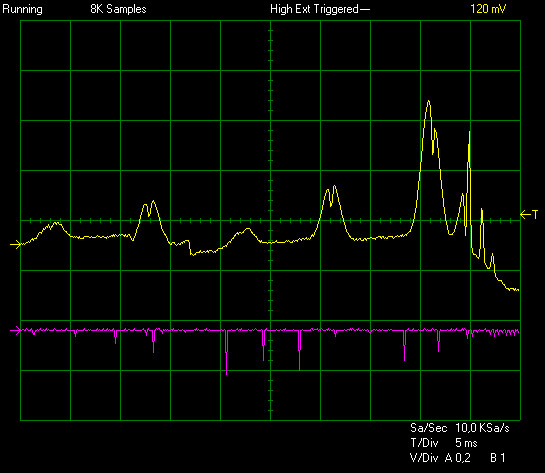
\includegraphics[width=\textwidth]{Figures/2/Tconst20C/117mA.jpg}
        \caption{$I=117$ mA}
        \label{fig:117mA}
    \end{subfigure}
    \begin{subfigure}[b]{0.3\textwidth}
        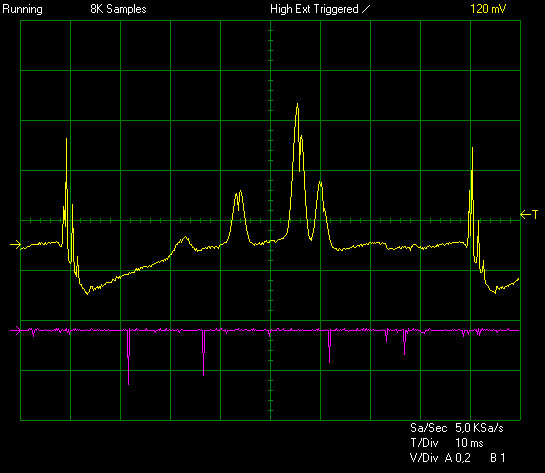
\includegraphics[width=\textwidth]{Figures/2/Tconst20C/118mA.jpg}
        \caption{$I=118$ mA}
        \label{fig:118mA}
    \end{subfigure}
    \begin{subfigure}[b]{0.3\textwidth}
        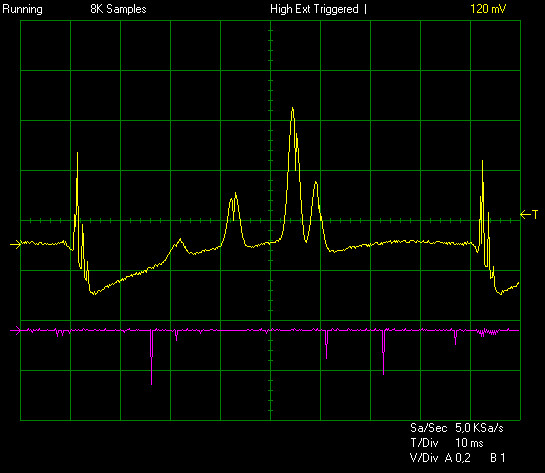
\includegraphics[width=\textwidth]{Figures/2/Tconst20C/119mA.jpg}
        \caption{$I=119$ mA}
        \label{fig:119mA}
    \end{subfigure}
    \begin{subfigure}[b]{0.3\textwidth}
        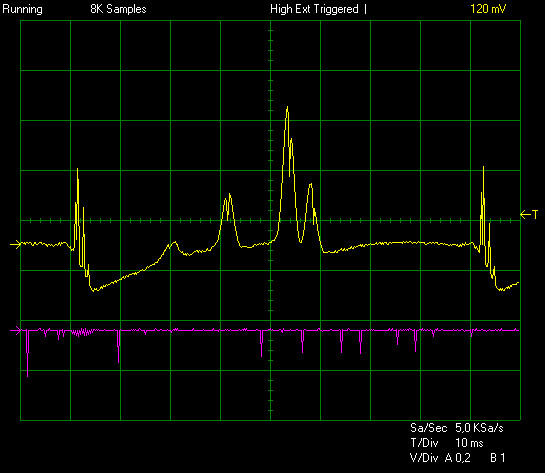
\includegraphics[width=\textwidth]{Figures/2/Tconst20C/120mA.jpg}
        \caption{$I=120$ mA}
        \label{fig:120mA}
    \end{subfigure}
    \begin{subfigure}[b]{0.3\textwidth}
        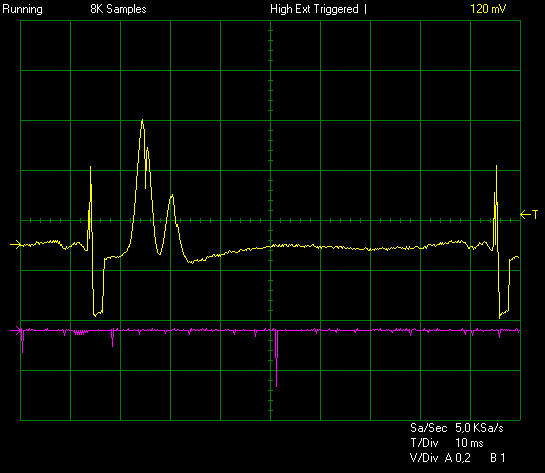
\includegraphics[width=\textwidth]{Figures/2/Tconst20C/121mA.jpg}
        \caption{$I=121$ mA}
        \label{fig:121mA}
    \end{subfigure}
    \begin{subfigure}[b]{0.3\textwidth}
        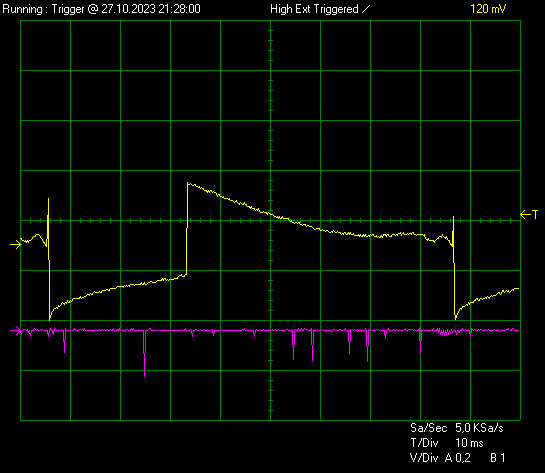
\includegraphics[width=\textwidth]{Figures/2/Tconst20C/122mA.jpg}
        \caption{$I=122$ mA}
        \label{fig:122mA}
    \end{subfigure}
    \caption{Saturation spectra for variation of injection currents}
    \label{fig:VariedCurrent}
\end{figure}

\pagebreak{}

For the case of constant injection current, a mode jump occurs between $T = \SI{19.9}{\celsius}$ and $T = \SI{20.1}{\celsius}$. We notice that changing the current affects the spectrum more drastically. This could be due to the fact that a slight change in the current leads to more heating compared to the temperature increments we used.

\begin{figure}[h]
    \centering
    \begin{subfigure}[b]{0.3\textwidth}
        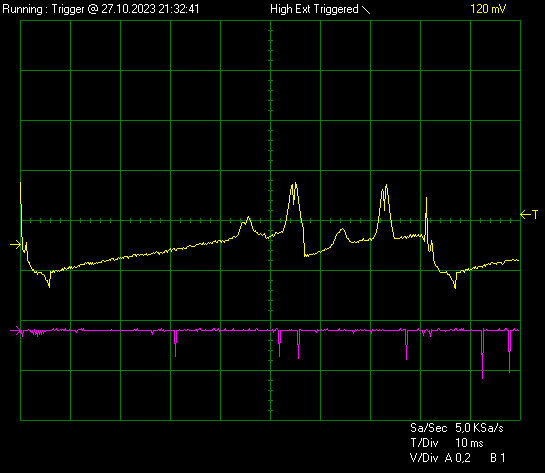
\includegraphics[width=\textwidth]{Figures/2/Iconst118mA/198.jpg}
        \caption{$T = \SI{19.8}{\celsius}$}
        \label{fig:198C}
    \end{subfigure}
    \begin{subfigure}[b]{0.3\textwidth}
        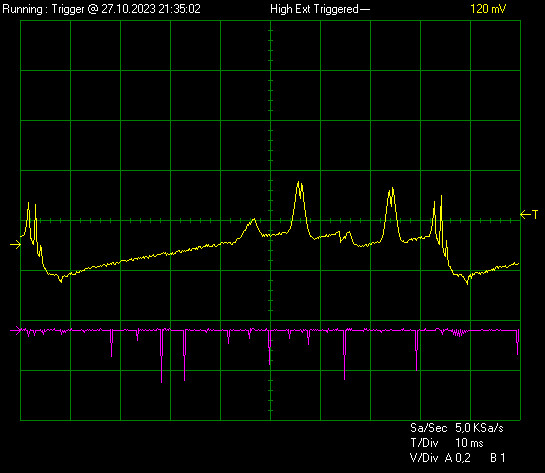
\includegraphics[width=\textwidth]{Figures/2/Iconst118mA/199.jpg}
        \caption{$T = \SI{19.9}{\celsius}$}
        \label{fig:199C}
    \end{subfigure}
    \begin{subfigure}[b]{0.3\textwidth}
        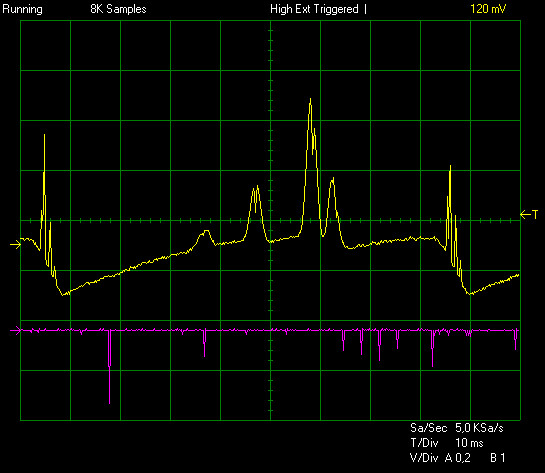
\includegraphics[width=\textwidth]{Figures/2/Iconst118mA/201.jpg}
        \caption{$T = \SI{20.1}{\celsius}$}
        \label{fig:201C}
    \end{subfigure}
    \begin{subfigure}[b]{0.3\textwidth}
        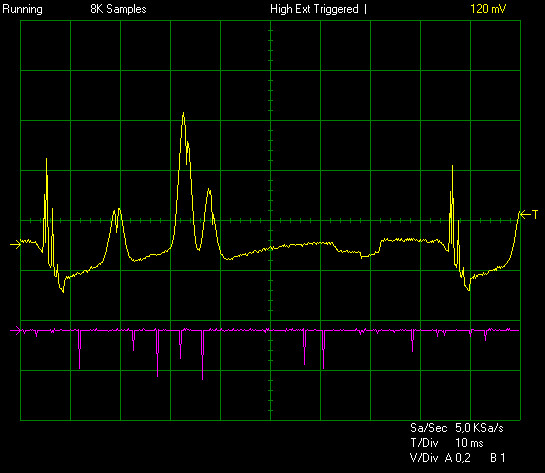
\includegraphics[width=\textwidth]{Figures/2/Iconst118mA/202.jpg}
        \caption{$T = \SI{20.2}{\celsius}$}
        \label{fig:202C}
    \end{subfigure}
    \begin{subfigure}[b]{0.3\textwidth}
        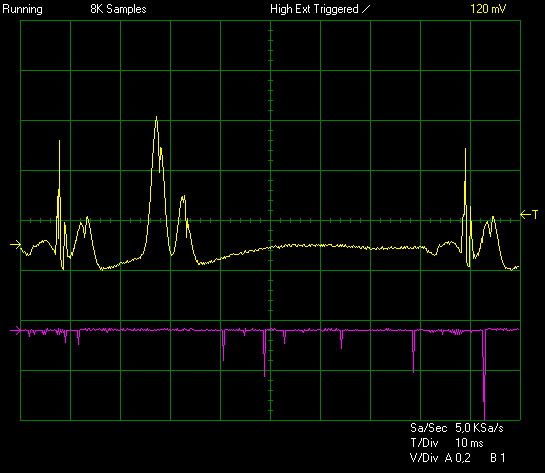
\includegraphics[width=\textwidth]{Figures/2/Iconst118mA/203.jpg}
        \caption{$T = \SI{20.3}{\celsius}$}
        \label{fig:203C}
    \end{subfigure}
    \caption{Saturation spectra for variation of temperature}
    \label{fig:VariedTemperature}
\end{figure}

\pagebreak{}

\subsection{Task 3}

In this task, we consider the effect of replacing the regular filter with a gradient filter at different orientations. We show the saturation spectra we obtained at different angles of the filter. 

\begin{figure}[h]
    \centering
    \begin{subfigure}[b]{0.3\textwidth}
        \centering
        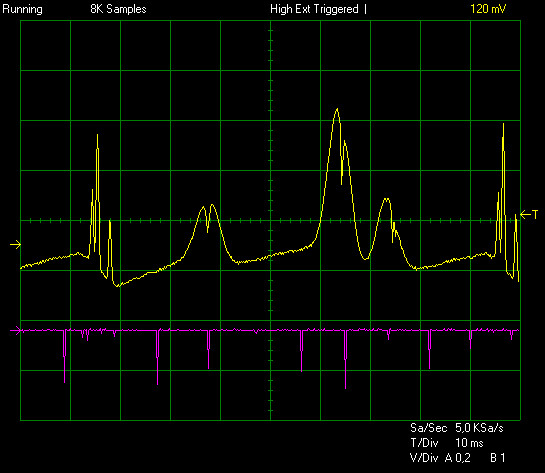
\includegraphics[width=\linewidth]{Figures/3/0deg.jpg}
        \caption{$\theta = \SI{0}{\degree}$}
        \label{fig:figure0}
    \end{subfigure}
    \begin{subfigure}[b]{0.3\textwidth}
        \centering
        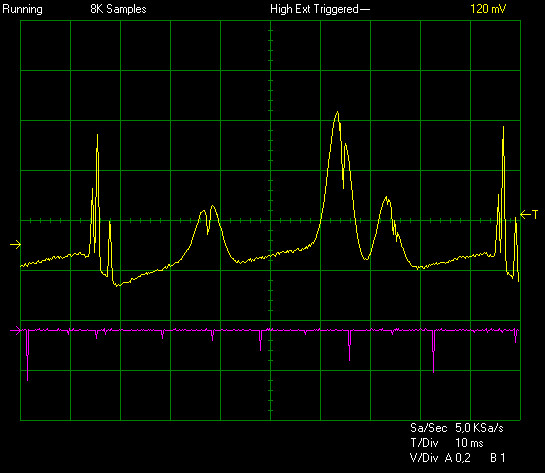
\includegraphics[width=\linewidth]{Figures/3/45deg.jpg}
        \caption{$\theta = \SI{45}{\degree}$}
        \label{fig:figure45}
    \end{subfigure}
    \begin{subfigure}[b]{0.3\textwidth}
        \centering
        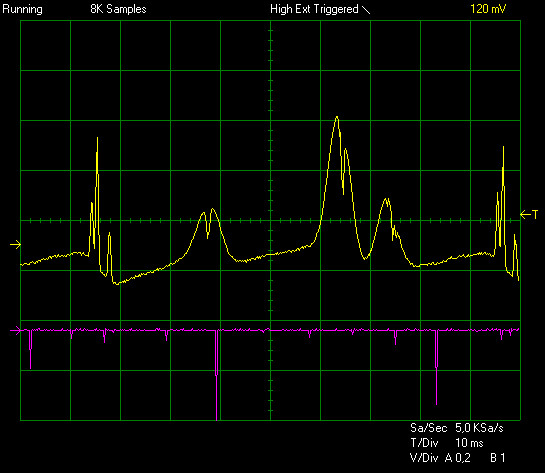
\includegraphics[width=\linewidth]{Figures/3/90deg.jpg}
        \caption{$\theta = \SI{90}{\degree}$}
        \label{fig:figure90}
    \end{subfigure}
    \begin{subfigure}[b]{0.3\textwidth}
        \centering
        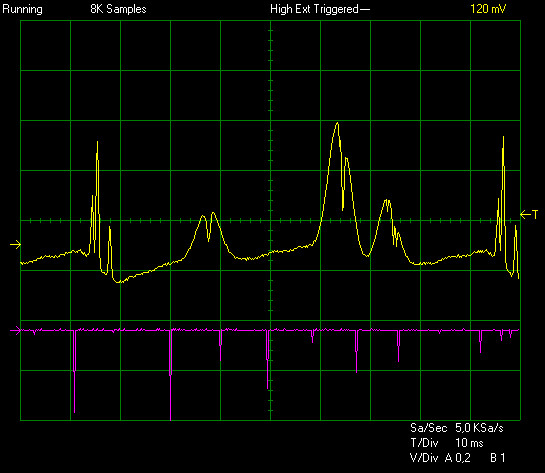
\includegraphics[width=\linewidth]{Figures/3/135deg.jpg}
        \caption{$\theta = \SI{135}{\degree}$}
        \label{fig:figure135}
    \end{subfigure}
    \begin{subfigure}[b]{0.3\textwidth}
        \centering
        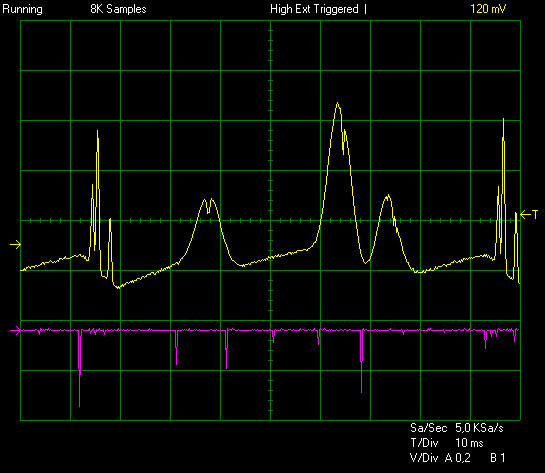
\includegraphics[width=\linewidth]{Figures/3/180deg.jpg}
        \caption{$\theta = \SI{180}{\degree}$}
        \label{fig:figure180}
    \end{subfigure}
    \begin{subfigure}[b]{0.3\textwidth}
        \centering
        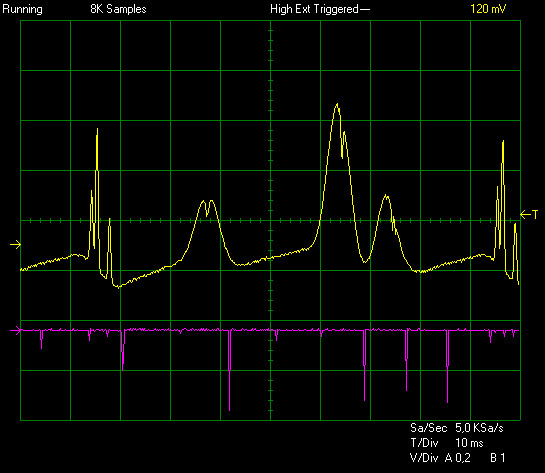
\includegraphics[width=\linewidth]{Figures/3/225deg.jpg}
        \caption{$\theta = \SI{225}{\degree}$}
        \label{fig:figure225}
    \end{subfigure}
    \begin{subfigure}[b]{0.3\textwidth}
        \centering
        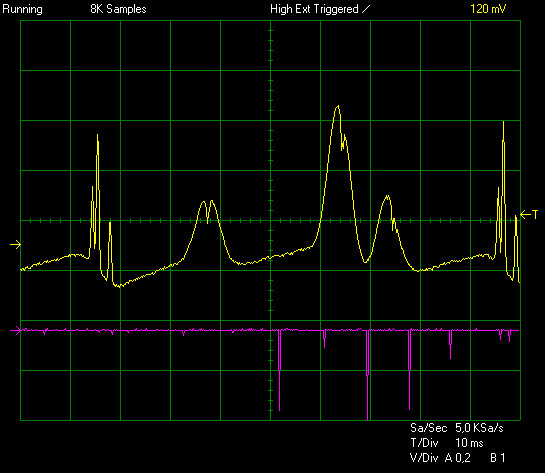
\includegraphics[width=\linewidth]{Figures/3/270deg.jpg}
        \caption{$\theta = \SI{270}{\degree}$}
        \label{fig:figure270}
    \end{subfigure}
    \begin{subfigure}[b]{0.3\textwidth}
        \centering
        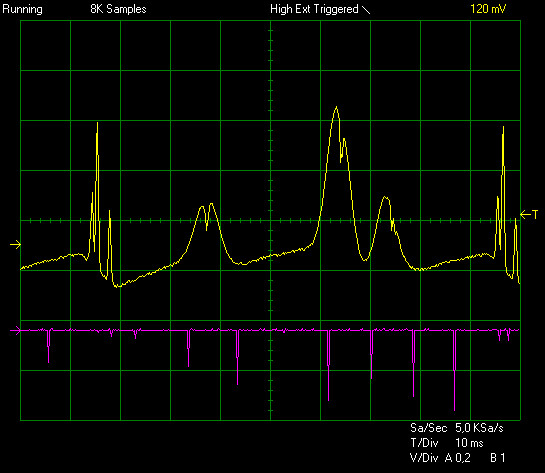
\includegraphics[width=\linewidth]{Figures/3/315deg.jpg}
        \caption{$\theta = \SI{315}{\degree}$}
        \label{fig:figure315}
    \end{subfigure}
    \begin{subfigure}[b]{0.3\textwidth}
        \centering
        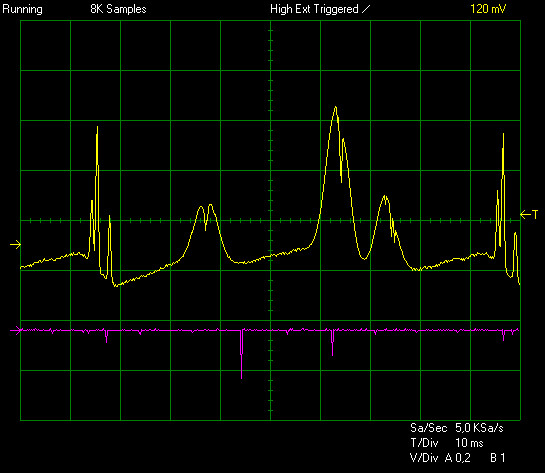
\includegraphics[width=\linewidth]{Figures/3/355deg.jpg}
        \caption{$\theta = \SI{355}{\degree}$}
        \label{fig:figure355}
    \end{subfigure}
    \caption{Saturation spectra for different angles}
    \label{fig:subfigures}
\end{figure}

The main observation is the decrease of peak heights as the filtering (i.e. the angle $\theta$) increases. No change was observed for the peak positions. This is due to the position of the filter in our setup. The filter only affects the probe beam and not the pump beam. Therefore, the proportion of population inversion stays the same while the intensity of the saturation peaks goes down. Moreover, the FPI peaks were not affected by changing the filtering. This is because the filter is placed after the beam splitter which controls how much of the initial beam goes into the interferometer. At $\theta=\SI{180}{\degree}$ a significant increase is observed. 

We also tested another filter which is thicker than the one we used and observed only a change in the intensity while all other aspects stayed invariant. A comparison of the thin vs thick filter is shown in the figure below. The spectrum looks different here because we are zoomed-in to a specific peak (peak 4) from the previous figures. 


\begin{figure}[h]
    \centering
    \begin{subfigure}[b]{0.3\textwidth}
        \centering
        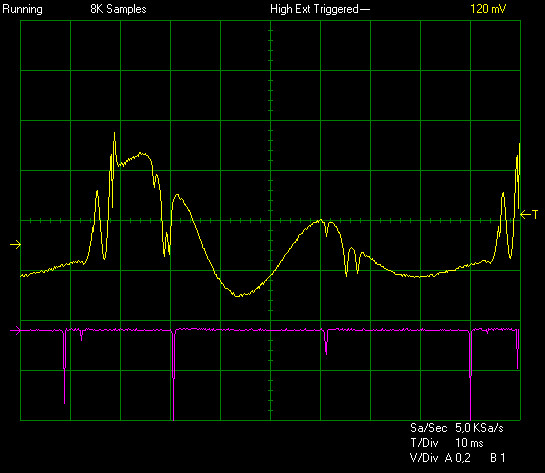
\includegraphics[width=\linewidth]{Figures/3/110ThinFilter.jpg}
        \caption{Thin filter}
        \label{fig:figure0}
    \end{subfigure}
    \begin{subfigure}[b]{0.3\textwidth}
        \centering
        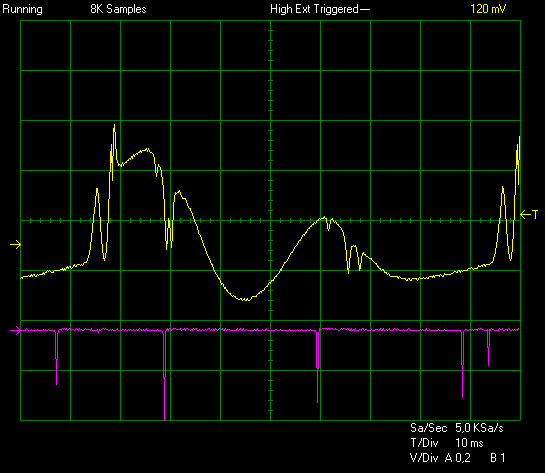
\includegraphics[width=\linewidth]{Figures/3/110ThickFilter.jpg}
        \caption{Thick filter}
        \label{fig:figure45}
    \end{subfigure}
\end{figure}

\pagebreak{}

\subsection{Task 4}

\textit{Fit the peaks in the absorption spectrum with a suitable fitting function. Extract
the characteristics of the individual peaks and compare them with literature values.}

In this part of the experiment, we recorded absorption and saturation spectra at two different currents. The following plot shows one of the spectra at 102 mA:

\begin{figure}[h]
    \centering
    %% Creator: Matplotlib, PGF backend
%%
%% To include the figure in your LaTeX document, write
%%   \input{<filename>.pgf}
%%
%% Make sure the required packages are loaded in your preamble
%%   \usepackage{pgf}
%%
%% Also ensure that all the required font packages are loaded; for instance,
%% the lmodern package is sometimes necessary when using math font.
%%   \usepackage{lmodern}
%%
%% Figures using additional raster images can only be included by \input if
%% they are in the same directory as the main LaTeX file. For loading figures
%% from other directories you can use the `import` package
%%   \usepackage{import}
%%
%% and then include the figures with
%%   \import{<path to file>}{<filename>.pgf}
%%
%% Matplotlib used the following preamble
%%   
%%   \usepackage{fontspec}
%%   \makeatletter\@ifpackageloaded{underscore}{}{\usepackage[strings]{underscore}}\makeatother
%%
\begingroup%
\makeatletter%
\begin{pgfpicture}%
\pgfpathrectangle{\pgfpointorigin}{\pgfqpoint{6.489553in}{4.010764in}}%
\pgfusepath{use as bounding box, clip}%
\begin{pgfscope}%
\pgfsetbuttcap%
\pgfsetmiterjoin%
\definecolor{currentfill}{rgb}{1.000000,1.000000,1.000000}%
\pgfsetfillcolor{currentfill}%
\pgfsetlinewidth{0.000000pt}%
\definecolor{currentstroke}{rgb}{1.000000,1.000000,1.000000}%
\pgfsetstrokecolor{currentstroke}%
\pgfsetdash{}{0pt}%
\pgfpathmoveto{\pgfqpoint{0.000000in}{0.000000in}}%
\pgfpathlineto{\pgfqpoint{6.489553in}{0.000000in}}%
\pgfpathlineto{\pgfqpoint{6.489553in}{4.010764in}}%
\pgfpathlineto{\pgfqpoint{0.000000in}{4.010764in}}%
\pgfpathlineto{\pgfqpoint{0.000000in}{0.000000in}}%
\pgfpathclose%
\pgfusepath{fill}%
\end{pgfscope}%
\begin{pgfscope}%
\pgfsetbuttcap%
\pgfsetmiterjoin%
\definecolor{currentfill}{rgb}{1.000000,1.000000,1.000000}%
\pgfsetfillcolor{currentfill}%
\pgfsetlinewidth{0.000000pt}%
\definecolor{currentstroke}{rgb}{0.000000,0.000000,0.000000}%
\pgfsetstrokecolor{currentstroke}%
\pgfsetstrokeopacity{0.000000}%
\pgfsetdash{}{0pt}%
\pgfpathmoveto{\pgfqpoint{0.811194in}{0.441184in}}%
\pgfpathlineto{\pgfqpoint{5.840598in}{0.441184in}}%
\pgfpathlineto{\pgfqpoint{5.840598in}{3.529473in}}%
\pgfpathlineto{\pgfqpoint{0.811194in}{3.529473in}}%
\pgfpathlineto{\pgfqpoint{0.811194in}{0.441184in}}%
\pgfpathclose%
\pgfusepath{fill}%
\end{pgfscope}%
\begin{pgfscope}%
\pgfsetbuttcap%
\pgfsetroundjoin%
\definecolor{currentfill}{rgb}{0.000000,0.000000,0.000000}%
\pgfsetfillcolor{currentfill}%
\pgfsetlinewidth{0.803000pt}%
\definecolor{currentstroke}{rgb}{0.000000,0.000000,0.000000}%
\pgfsetstrokecolor{currentstroke}%
\pgfsetdash{}{0pt}%
\pgfsys@defobject{currentmarker}{\pgfqpoint{0.000000in}{-0.048611in}}{\pgfqpoint{0.000000in}{0.000000in}}{%
\pgfpathmoveto{\pgfqpoint{0.000000in}{0.000000in}}%
\pgfpathlineto{\pgfqpoint{0.000000in}{-0.048611in}}%
\pgfusepath{stroke,fill}%
}%
\begin{pgfscope}%
\pgfsys@transformshift{1.327762in}{0.441184in}%
\pgfsys@useobject{currentmarker}{}%
\end{pgfscope}%
\end{pgfscope}%
\begin{pgfscope}%
\definecolor{textcolor}{rgb}{0.000000,0.000000,0.000000}%
\pgfsetstrokecolor{textcolor}%
\pgfsetfillcolor{textcolor}%
\pgftext[x=1.327762in,y=0.343962in,,top]{\color{textcolor}\rmfamily\fontsize{10.000000}{12.000000}\selectfont \(\displaystyle {3}\)}%
\end{pgfscope}%
\begin{pgfscope}%
\pgfsetbuttcap%
\pgfsetroundjoin%
\definecolor{currentfill}{rgb}{0.000000,0.000000,0.000000}%
\pgfsetfillcolor{currentfill}%
\pgfsetlinewidth{0.803000pt}%
\definecolor{currentstroke}{rgb}{0.000000,0.000000,0.000000}%
\pgfsetstrokecolor{currentstroke}%
\pgfsetdash{}{0pt}%
\pgfsys@defobject{currentmarker}{\pgfqpoint{0.000000in}{-0.048611in}}{\pgfqpoint{0.000000in}{0.000000in}}{%
\pgfpathmoveto{\pgfqpoint{0.000000in}{0.000000in}}%
\pgfpathlineto{\pgfqpoint{0.000000in}{-0.048611in}}%
\pgfusepath{stroke,fill}%
}%
\begin{pgfscope}%
\pgfsys@transformshift{1.919069in}{0.441184in}%
\pgfsys@useobject{currentmarker}{}%
\end{pgfscope}%
\end{pgfscope}%
\begin{pgfscope}%
\definecolor{textcolor}{rgb}{0.000000,0.000000,0.000000}%
\pgfsetstrokecolor{textcolor}%
\pgfsetfillcolor{textcolor}%
\pgftext[x=1.919069in,y=0.343962in,,top]{\color{textcolor}\rmfamily\fontsize{10.000000}{12.000000}\selectfont \(\displaystyle {4}\)}%
\end{pgfscope}%
\begin{pgfscope}%
\pgfsetbuttcap%
\pgfsetroundjoin%
\definecolor{currentfill}{rgb}{0.000000,0.000000,0.000000}%
\pgfsetfillcolor{currentfill}%
\pgfsetlinewidth{0.803000pt}%
\definecolor{currentstroke}{rgb}{0.000000,0.000000,0.000000}%
\pgfsetstrokecolor{currentstroke}%
\pgfsetdash{}{0pt}%
\pgfsys@defobject{currentmarker}{\pgfqpoint{0.000000in}{-0.048611in}}{\pgfqpoint{0.000000in}{0.000000in}}{%
\pgfpathmoveto{\pgfqpoint{0.000000in}{0.000000in}}%
\pgfpathlineto{\pgfqpoint{0.000000in}{-0.048611in}}%
\pgfusepath{stroke,fill}%
}%
\begin{pgfscope}%
\pgfsys@transformshift{2.510375in}{0.441184in}%
\pgfsys@useobject{currentmarker}{}%
\end{pgfscope}%
\end{pgfscope}%
\begin{pgfscope}%
\definecolor{textcolor}{rgb}{0.000000,0.000000,0.000000}%
\pgfsetstrokecolor{textcolor}%
\pgfsetfillcolor{textcolor}%
\pgftext[x=2.510375in,y=0.343962in,,top]{\color{textcolor}\rmfamily\fontsize{10.000000}{12.000000}\selectfont \(\displaystyle {5}\)}%
\end{pgfscope}%
\begin{pgfscope}%
\pgfsetbuttcap%
\pgfsetroundjoin%
\definecolor{currentfill}{rgb}{0.000000,0.000000,0.000000}%
\pgfsetfillcolor{currentfill}%
\pgfsetlinewidth{0.803000pt}%
\definecolor{currentstroke}{rgb}{0.000000,0.000000,0.000000}%
\pgfsetstrokecolor{currentstroke}%
\pgfsetdash{}{0pt}%
\pgfsys@defobject{currentmarker}{\pgfqpoint{0.000000in}{-0.048611in}}{\pgfqpoint{0.000000in}{0.000000in}}{%
\pgfpathmoveto{\pgfqpoint{0.000000in}{0.000000in}}%
\pgfpathlineto{\pgfqpoint{0.000000in}{-0.048611in}}%
\pgfusepath{stroke,fill}%
}%
\begin{pgfscope}%
\pgfsys@transformshift{3.101681in}{0.441184in}%
\pgfsys@useobject{currentmarker}{}%
\end{pgfscope}%
\end{pgfscope}%
\begin{pgfscope}%
\definecolor{textcolor}{rgb}{0.000000,0.000000,0.000000}%
\pgfsetstrokecolor{textcolor}%
\pgfsetfillcolor{textcolor}%
\pgftext[x=3.101681in,y=0.343962in,,top]{\color{textcolor}\rmfamily\fontsize{10.000000}{12.000000}\selectfont \(\displaystyle {6}\)}%
\end{pgfscope}%
\begin{pgfscope}%
\pgfsetbuttcap%
\pgfsetroundjoin%
\definecolor{currentfill}{rgb}{0.000000,0.000000,0.000000}%
\pgfsetfillcolor{currentfill}%
\pgfsetlinewidth{0.803000pt}%
\definecolor{currentstroke}{rgb}{0.000000,0.000000,0.000000}%
\pgfsetstrokecolor{currentstroke}%
\pgfsetdash{}{0pt}%
\pgfsys@defobject{currentmarker}{\pgfqpoint{0.000000in}{-0.048611in}}{\pgfqpoint{0.000000in}{0.000000in}}{%
\pgfpathmoveto{\pgfqpoint{0.000000in}{0.000000in}}%
\pgfpathlineto{\pgfqpoint{0.000000in}{-0.048611in}}%
\pgfusepath{stroke,fill}%
}%
\begin{pgfscope}%
\pgfsys@transformshift{3.692988in}{0.441184in}%
\pgfsys@useobject{currentmarker}{}%
\end{pgfscope}%
\end{pgfscope}%
\begin{pgfscope}%
\definecolor{textcolor}{rgb}{0.000000,0.000000,0.000000}%
\pgfsetstrokecolor{textcolor}%
\pgfsetfillcolor{textcolor}%
\pgftext[x=3.692988in,y=0.343962in,,top]{\color{textcolor}\rmfamily\fontsize{10.000000}{12.000000}\selectfont \(\displaystyle {7}\)}%
\end{pgfscope}%
\begin{pgfscope}%
\pgfsetbuttcap%
\pgfsetroundjoin%
\definecolor{currentfill}{rgb}{0.000000,0.000000,0.000000}%
\pgfsetfillcolor{currentfill}%
\pgfsetlinewidth{0.803000pt}%
\definecolor{currentstroke}{rgb}{0.000000,0.000000,0.000000}%
\pgfsetstrokecolor{currentstroke}%
\pgfsetdash{}{0pt}%
\pgfsys@defobject{currentmarker}{\pgfqpoint{0.000000in}{-0.048611in}}{\pgfqpoint{0.000000in}{0.000000in}}{%
\pgfpathmoveto{\pgfqpoint{0.000000in}{0.000000in}}%
\pgfpathlineto{\pgfqpoint{0.000000in}{-0.048611in}}%
\pgfusepath{stroke,fill}%
}%
\begin{pgfscope}%
\pgfsys@transformshift{4.284294in}{0.441184in}%
\pgfsys@useobject{currentmarker}{}%
\end{pgfscope}%
\end{pgfscope}%
\begin{pgfscope}%
\definecolor{textcolor}{rgb}{0.000000,0.000000,0.000000}%
\pgfsetstrokecolor{textcolor}%
\pgfsetfillcolor{textcolor}%
\pgftext[x=4.284294in,y=0.343962in,,top]{\color{textcolor}\rmfamily\fontsize{10.000000}{12.000000}\selectfont \(\displaystyle {8}\)}%
\end{pgfscope}%
\begin{pgfscope}%
\pgfsetbuttcap%
\pgfsetroundjoin%
\definecolor{currentfill}{rgb}{0.000000,0.000000,0.000000}%
\pgfsetfillcolor{currentfill}%
\pgfsetlinewidth{0.803000pt}%
\definecolor{currentstroke}{rgb}{0.000000,0.000000,0.000000}%
\pgfsetstrokecolor{currentstroke}%
\pgfsetdash{}{0pt}%
\pgfsys@defobject{currentmarker}{\pgfqpoint{0.000000in}{-0.048611in}}{\pgfqpoint{0.000000in}{0.000000in}}{%
\pgfpathmoveto{\pgfqpoint{0.000000in}{0.000000in}}%
\pgfpathlineto{\pgfqpoint{0.000000in}{-0.048611in}}%
\pgfusepath{stroke,fill}%
}%
\begin{pgfscope}%
\pgfsys@transformshift{4.875601in}{0.441184in}%
\pgfsys@useobject{currentmarker}{}%
\end{pgfscope}%
\end{pgfscope}%
\begin{pgfscope}%
\definecolor{textcolor}{rgb}{0.000000,0.000000,0.000000}%
\pgfsetstrokecolor{textcolor}%
\pgfsetfillcolor{textcolor}%
\pgftext[x=4.875601in,y=0.343962in,,top]{\color{textcolor}\rmfamily\fontsize{10.000000}{12.000000}\selectfont \(\displaystyle {9}\)}%
\end{pgfscope}%
\begin{pgfscope}%
\pgfsetbuttcap%
\pgfsetroundjoin%
\definecolor{currentfill}{rgb}{0.000000,0.000000,0.000000}%
\pgfsetfillcolor{currentfill}%
\pgfsetlinewidth{0.803000pt}%
\definecolor{currentstroke}{rgb}{0.000000,0.000000,0.000000}%
\pgfsetstrokecolor{currentstroke}%
\pgfsetdash{}{0pt}%
\pgfsys@defobject{currentmarker}{\pgfqpoint{0.000000in}{-0.048611in}}{\pgfqpoint{0.000000in}{0.000000in}}{%
\pgfpathmoveto{\pgfqpoint{0.000000in}{0.000000in}}%
\pgfpathlineto{\pgfqpoint{0.000000in}{-0.048611in}}%
\pgfusepath{stroke,fill}%
}%
\begin{pgfscope}%
\pgfsys@transformshift{5.466907in}{0.441184in}%
\pgfsys@useobject{currentmarker}{}%
\end{pgfscope}%
\end{pgfscope}%
\begin{pgfscope}%
\definecolor{textcolor}{rgb}{0.000000,0.000000,0.000000}%
\pgfsetstrokecolor{textcolor}%
\pgfsetfillcolor{textcolor}%
\pgftext[x=5.466907in,y=0.343962in,,top]{\color{textcolor}\rmfamily\fontsize{10.000000}{12.000000}\selectfont \(\displaystyle {10}\)}%
\end{pgfscope}%
\begin{pgfscope}%
\definecolor{textcolor}{rgb}{0.000000,0.000000,0.000000}%
\pgfsetstrokecolor{textcolor}%
\pgfsetfillcolor{textcolor}%
\pgftext[x=3.325896in,y=0.165073in,,top]{\color{textcolor}\rmfamily\fontsize{10.000000}{12.000000}\selectfont Frequency [GHz]}%
\end{pgfscope}%
\begin{pgfscope}%
\pgfsetbuttcap%
\pgfsetroundjoin%
\definecolor{currentfill}{rgb}{0.000000,0.000000,0.000000}%
\pgfsetfillcolor{currentfill}%
\pgfsetlinewidth{0.803000pt}%
\definecolor{currentstroke}{rgb}{0.000000,0.000000,0.000000}%
\pgfsetstrokecolor{currentstroke}%
\pgfsetdash{}{0pt}%
\pgfsys@defobject{currentmarker}{\pgfqpoint{-0.048611in}{0.000000in}}{\pgfqpoint{-0.000000in}{0.000000in}}{%
\pgfpathmoveto{\pgfqpoint{-0.000000in}{0.000000in}}%
\pgfpathlineto{\pgfqpoint{-0.048611in}{0.000000in}}%
\pgfusepath{stroke,fill}%
}%
\begin{pgfscope}%
\pgfsys@transformshift{0.811194in}{0.661425in}%
\pgfsys@useobject{currentmarker}{}%
\end{pgfscope}%
\end{pgfscope}%
\begin{pgfscope}%
\definecolor{textcolor}{rgb}{0.000000,0.000000,0.000000}%
\pgfsetstrokecolor{textcolor}%
\pgfsetfillcolor{textcolor}%
\pgftext[x=0.536502in, y=0.613231in, left, base]{\color{textcolor}\rmfamily\fontsize{10.000000}{12.000000}\selectfont \(\displaystyle {\ensuremath{-}2}\)}%
\end{pgfscope}%
\begin{pgfscope}%
\pgfsetbuttcap%
\pgfsetroundjoin%
\definecolor{currentfill}{rgb}{0.000000,0.000000,0.000000}%
\pgfsetfillcolor{currentfill}%
\pgfsetlinewidth{0.803000pt}%
\definecolor{currentstroke}{rgb}{0.000000,0.000000,0.000000}%
\pgfsetstrokecolor{currentstroke}%
\pgfsetdash{}{0pt}%
\pgfsys@defobject{currentmarker}{\pgfqpoint{-0.048611in}{0.000000in}}{\pgfqpoint{-0.000000in}{0.000000in}}{%
\pgfpathmoveto{\pgfqpoint{-0.000000in}{0.000000in}}%
\pgfpathlineto{\pgfqpoint{-0.048611in}{0.000000in}}%
\pgfusepath{stroke,fill}%
}%
\begin{pgfscope}%
\pgfsys@transformshift{0.811194in}{1.275765in}%
\pgfsys@useobject{currentmarker}{}%
\end{pgfscope}%
\end{pgfscope}%
\begin{pgfscope}%
\definecolor{textcolor}{rgb}{0.000000,0.000000,0.000000}%
\pgfsetstrokecolor{textcolor}%
\pgfsetfillcolor{textcolor}%
\pgftext[x=0.644527in, y=1.227571in, left, base]{\color{textcolor}\rmfamily\fontsize{10.000000}{12.000000}\selectfont \(\displaystyle {0}\)}%
\end{pgfscope}%
\begin{pgfscope}%
\pgfsetbuttcap%
\pgfsetroundjoin%
\definecolor{currentfill}{rgb}{0.000000,0.000000,0.000000}%
\pgfsetfillcolor{currentfill}%
\pgfsetlinewidth{0.803000pt}%
\definecolor{currentstroke}{rgb}{0.000000,0.000000,0.000000}%
\pgfsetstrokecolor{currentstroke}%
\pgfsetdash{}{0pt}%
\pgfsys@defobject{currentmarker}{\pgfqpoint{-0.048611in}{0.000000in}}{\pgfqpoint{-0.000000in}{0.000000in}}{%
\pgfpathmoveto{\pgfqpoint{-0.000000in}{0.000000in}}%
\pgfpathlineto{\pgfqpoint{-0.048611in}{0.000000in}}%
\pgfusepath{stroke,fill}%
}%
\begin{pgfscope}%
\pgfsys@transformshift{0.811194in}{1.890106in}%
\pgfsys@useobject{currentmarker}{}%
\end{pgfscope}%
\end{pgfscope}%
\begin{pgfscope}%
\definecolor{textcolor}{rgb}{0.000000,0.000000,0.000000}%
\pgfsetstrokecolor{textcolor}%
\pgfsetfillcolor{textcolor}%
\pgftext[x=0.644527in, y=1.841911in, left, base]{\color{textcolor}\rmfamily\fontsize{10.000000}{12.000000}\selectfont \(\displaystyle {2}\)}%
\end{pgfscope}%
\begin{pgfscope}%
\pgfsetbuttcap%
\pgfsetroundjoin%
\definecolor{currentfill}{rgb}{0.000000,0.000000,0.000000}%
\pgfsetfillcolor{currentfill}%
\pgfsetlinewidth{0.803000pt}%
\definecolor{currentstroke}{rgb}{0.000000,0.000000,0.000000}%
\pgfsetstrokecolor{currentstroke}%
\pgfsetdash{}{0pt}%
\pgfsys@defobject{currentmarker}{\pgfqpoint{-0.048611in}{0.000000in}}{\pgfqpoint{-0.000000in}{0.000000in}}{%
\pgfpathmoveto{\pgfqpoint{-0.000000in}{0.000000in}}%
\pgfpathlineto{\pgfqpoint{-0.048611in}{0.000000in}}%
\pgfusepath{stroke,fill}%
}%
\begin{pgfscope}%
\pgfsys@transformshift{0.811194in}{2.504446in}%
\pgfsys@useobject{currentmarker}{}%
\end{pgfscope}%
\end{pgfscope}%
\begin{pgfscope}%
\definecolor{textcolor}{rgb}{0.000000,0.000000,0.000000}%
\pgfsetstrokecolor{textcolor}%
\pgfsetfillcolor{textcolor}%
\pgftext[x=0.644527in, y=2.456251in, left, base]{\color{textcolor}\rmfamily\fontsize{10.000000}{12.000000}\selectfont \(\displaystyle {4}\)}%
\end{pgfscope}%
\begin{pgfscope}%
\pgfsetbuttcap%
\pgfsetroundjoin%
\definecolor{currentfill}{rgb}{0.000000,0.000000,0.000000}%
\pgfsetfillcolor{currentfill}%
\pgfsetlinewidth{0.803000pt}%
\definecolor{currentstroke}{rgb}{0.000000,0.000000,0.000000}%
\pgfsetstrokecolor{currentstroke}%
\pgfsetdash{}{0pt}%
\pgfsys@defobject{currentmarker}{\pgfqpoint{-0.048611in}{0.000000in}}{\pgfqpoint{-0.000000in}{0.000000in}}{%
\pgfpathmoveto{\pgfqpoint{-0.000000in}{0.000000in}}%
\pgfpathlineto{\pgfqpoint{-0.048611in}{0.000000in}}%
\pgfusepath{stroke,fill}%
}%
\begin{pgfscope}%
\pgfsys@transformshift{0.811194in}{3.118786in}%
\pgfsys@useobject{currentmarker}{}%
\end{pgfscope}%
\end{pgfscope}%
\begin{pgfscope}%
\definecolor{textcolor}{rgb}{0.000000,0.000000,0.000000}%
\pgfsetstrokecolor{textcolor}%
\pgfsetfillcolor{textcolor}%
\pgftext[x=0.644527in, y=3.070592in, left, base]{\color{textcolor}\rmfamily\fontsize{10.000000}{12.000000}\selectfont \(\displaystyle {6}\)}%
\end{pgfscope}%
\begin{pgfscope}%
\definecolor{textcolor}{rgb}{0.000000,0.000000,0.000000}%
\pgfsetstrokecolor{textcolor}%
\pgfsetfillcolor{textcolor}%
\pgftext[x=0.480947in,y=1.985328in,,bottom,rotate=90.000000]{\color{textcolor}\rmfamily\fontsize{10.000000}{12.000000}\selectfont Intensity [a.u.]}%
\end{pgfscope}%
\begin{pgfscope}%
\pgfpathrectangle{\pgfqpoint{0.811194in}{0.441184in}}{\pgfqpoint{5.029404in}{3.088289in}}%
\pgfusepath{clip}%
\pgfsetrectcap%
\pgfsetroundjoin%
\pgfsetlinewidth{1.505625pt}%
\definecolor{currentstroke}{rgb}{0.000000,0.000000,1.000000}%
\pgfsetstrokecolor{currentstroke}%
\pgfsetdash{}{0pt}%
\pgfpathmoveto{\pgfqpoint{0.801194in}{0.807753in}}%
\pgfpathlineto{\pgfqpoint{0.811194in}{0.827297in}}%
\pgfpathlineto{\pgfqpoint{0.826911in}{0.821154in}}%
\pgfpathlineto{\pgfqpoint{0.842628in}{0.851871in}}%
\pgfpathlineto{\pgfqpoint{0.858345in}{0.833440in}}%
\pgfpathlineto{\pgfqpoint{0.874062in}{0.858014in}}%
\pgfpathlineto{\pgfqpoint{0.889779in}{0.870301in}}%
\pgfpathlineto{\pgfqpoint{0.905495in}{0.888731in}}%
\pgfpathlineto{\pgfqpoint{0.936929in}{0.901018in}}%
\pgfpathlineto{\pgfqpoint{0.952646in}{0.913305in}}%
\pgfpathlineto{\pgfqpoint{0.968363in}{0.950165in}}%
\pgfpathlineto{\pgfqpoint{0.984080in}{0.974739in}}%
\pgfpathlineto{\pgfqpoint{0.999797in}{0.993169in}}%
\pgfpathlineto{\pgfqpoint{1.015514in}{1.023886in}}%
\pgfpathlineto{\pgfqpoint{1.031231in}{1.030029in}}%
\pgfpathlineto{\pgfqpoint{1.046947in}{1.079176in}}%
\pgfpathlineto{\pgfqpoint{1.062664in}{1.091463in}}%
\pgfpathlineto{\pgfqpoint{1.078381in}{1.116037in}}%
\pgfpathlineto{\pgfqpoint{1.094098in}{1.122180in}}%
\pgfpathlineto{\pgfqpoint{1.109815in}{1.165184in}}%
\pgfpathlineto{\pgfqpoint{1.125532in}{1.177471in}}%
\pgfpathlineto{\pgfqpoint{1.156966in}{1.214331in}}%
\pgfpathlineto{\pgfqpoint{1.172683in}{1.238905in}}%
\pgfpathlineto{\pgfqpoint{1.188399in}{1.251192in}}%
\pgfpathlineto{\pgfqpoint{1.235550in}{1.269622in}}%
\pgfpathlineto{\pgfqpoint{1.251267in}{1.281909in}}%
\pgfpathlineto{\pgfqpoint{1.266984in}{1.275765in}}%
\pgfpathlineto{\pgfqpoint{1.282701in}{1.288052in}}%
\pgfpathlineto{\pgfqpoint{1.298418in}{1.294196in}}%
\pgfpathlineto{\pgfqpoint{1.314134in}{1.269622in}}%
\pgfpathlineto{\pgfqpoint{1.329851in}{1.257335in}}%
\pgfpathlineto{\pgfqpoint{1.345568in}{1.251192in}}%
\pgfpathlineto{\pgfqpoint{1.361285in}{1.238905in}}%
\pgfpathlineto{\pgfqpoint{1.377002in}{1.208188in}}%
\pgfpathlineto{\pgfqpoint{1.392719in}{1.189758in}}%
\pgfpathlineto{\pgfqpoint{1.408436in}{1.177471in}}%
\pgfpathlineto{\pgfqpoint{1.424153in}{1.177471in}}%
\pgfpathlineto{\pgfqpoint{1.439870in}{1.116037in}}%
\pgfpathlineto{\pgfqpoint{1.455586in}{1.103750in}}%
\pgfpathlineto{\pgfqpoint{1.471303in}{1.109893in}}%
\pgfpathlineto{\pgfqpoint{1.502737in}{1.048459in}}%
\pgfpathlineto{\pgfqpoint{1.518454in}{1.054603in}}%
\pgfpathlineto{\pgfqpoint{1.534171in}{1.023886in}}%
\pgfpathlineto{\pgfqpoint{1.549888in}{1.030029in}}%
\pgfpathlineto{\pgfqpoint{1.565605in}{0.999312in}}%
\pgfpathlineto{\pgfqpoint{1.581322in}{0.999312in}}%
\pgfpathlineto{\pgfqpoint{1.597038in}{1.011599in}}%
\pgfpathlineto{\pgfqpoint{1.644189in}{0.993169in}}%
\pgfpathlineto{\pgfqpoint{1.659906in}{0.980882in}}%
\pgfpathlineto{\pgfqpoint{1.675623in}{0.980882in}}%
\pgfpathlineto{\pgfqpoint{1.691340in}{0.962452in}}%
\pgfpathlineto{\pgfqpoint{1.707057in}{0.974739in}}%
\pgfpathlineto{\pgfqpoint{1.722774in}{0.968595in}}%
\pgfpathlineto{\pgfqpoint{1.738490in}{0.974739in}}%
\pgfpathlineto{\pgfqpoint{1.754207in}{0.999312in}}%
\pgfpathlineto{\pgfqpoint{1.769924in}{1.005456in}}%
\pgfpathlineto{\pgfqpoint{1.785641in}{1.005456in}}%
\pgfpathlineto{\pgfqpoint{1.801358in}{0.974739in}}%
\pgfpathlineto{\pgfqpoint{1.817075in}{1.011599in}}%
\pgfpathlineto{\pgfqpoint{1.832792in}{0.999312in}}%
\pgfpathlineto{\pgfqpoint{1.848509in}{1.017742in}}%
\pgfpathlineto{\pgfqpoint{1.864226in}{0.999312in}}%
\pgfpathlineto{\pgfqpoint{1.879942in}{1.011599in}}%
\pgfpathlineto{\pgfqpoint{1.895659in}{1.030029in}}%
\pgfpathlineto{\pgfqpoint{1.911376in}{1.036173in}}%
\pgfpathlineto{\pgfqpoint{1.927093in}{1.011599in}}%
\pgfpathlineto{\pgfqpoint{1.942810in}{1.036173in}}%
\pgfpathlineto{\pgfqpoint{1.958527in}{1.030029in}}%
\pgfpathlineto{\pgfqpoint{1.974244in}{1.048459in}}%
\pgfpathlineto{\pgfqpoint{2.005677in}{1.036173in}}%
\pgfpathlineto{\pgfqpoint{2.021394in}{1.048459in}}%
\pgfpathlineto{\pgfqpoint{2.037111in}{1.048459in}}%
\pgfpathlineto{\pgfqpoint{2.052828in}{1.060746in}}%
\pgfpathlineto{\pgfqpoint{2.068545in}{1.060746in}}%
\pgfpathlineto{\pgfqpoint{2.131413in}{1.085320in}}%
\pgfpathlineto{\pgfqpoint{2.147129in}{1.085320in}}%
\pgfpathlineto{\pgfqpoint{2.162846in}{1.109893in}}%
\pgfpathlineto{\pgfqpoint{2.178563in}{1.103750in}}%
\pgfpathlineto{\pgfqpoint{2.194280in}{1.122180in}}%
\pgfpathlineto{\pgfqpoint{2.209997in}{1.128324in}}%
\pgfpathlineto{\pgfqpoint{2.225714in}{1.128324in}}%
\pgfpathlineto{\pgfqpoint{2.241431in}{1.122180in}}%
\pgfpathlineto{\pgfqpoint{2.272865in}{1.146754in}}%
\pgfpathlineto{\pgfqpoint{2.288581in}{1.128324in}}%
\pgfpathlineto{\pgfqpoint{2.304298in}{1.152897in}}%
\pgfpathlineto{\pgfqpoint{2.320015in}{1.134467in}}%
\pgfpathlineto{\pgfqpoint{2.335732in}{1.146754in}}%
\pgfpathlineto{\pgfqpoint{2.351449in}{1.140610in}}%
\pgfpathlineto{\pgfqpoint{2.367166in}{1.171327in}}%
\pgfpathlineto{\pgfqpoint{2.382883in}{1.165184in}}%
\pgfpathlineto{\pgfqpoint{2.398600in}{1.195901in}}%
\pgfpathlineto{\pgfqpoint{2.414317in}{1.183614in}}%
\pgfpathlineto{\pgfqpoint{2.430033in}{1.189758in}}%
\pgfpathlineto{\pgfqpoint{2.445750in}{1.189758in}}%
\pgfpathlineto{\pgfqpoint{2.461467in}{1.208188in}}%
\pgfpathlineto{\pgfqpoint{2.477184in}{1.214331in}}%
\pgfpathlineto{\pgfqpoint{2.492901in}{1.251192in}}%
\pgfpathlineto{\pgfqpoint{2.508618in}{1.281909in}}%
\pgfpathlineto{\pgfqpoint{2.524335in}{1.306482in}}%
\pgfpathlineto{\pgfqpoint{2.555769in}{1.380203in}}%
\pgfpathlineto{\pgfqpoint{2.571485in}{1.404777in}}%
\pgfpathlineto{\pgfqpoint{2.587202in}{1.478498in}}%
\pgfpathlineto{\pgfqpoint{2.618636in}{1.576792in}}%
\pgfpathlineto{\pgfqpoint{2.634353in}{1.656656in}}%
\pgfpathlineto{\pgfqpoint{2.650070in}{1.699660in}}%
\pgfpathlineto{\pgfqpoint{2.665787in}{1.767238in}}%
\pgfpathlineto{\pgfqpoint{2.681504in}{1.853245in}}%
\pgfpathlineto{\pgfqpoint{2.697220in}{1.926966in}}%
\pgfpathlineto{\pgfqpoint{2.712937in}{1.994543in}}%
\pgfpathlineto{\pgfqpoint{2.728654in}{2.043691in}}%
\pgfpathlineto{\pgfqpoint{2.744371in}{2.080551in}}%
\pgfpathlineto{\pgfqpoint{2.760088in}{2.123555in}}%
\pgfpathlineto{\pgfqpoint{2.775805in}{2.154272in}}%
\pgfpathlineto{\pgfqpoint{2.791522in}{2.129698in}}%
\pgfpathlineto{\pgfqpoint{2.807239in}{2.092838in}}%
\pgfpathlineto{\pgfqpoint{2.822956in}{2.135842in}}%
\pgfpathlineto{\pgfqpoint{2.838672in}{2.154272in}}%
\pgfpathlineto{\pgfqpoint{2.854389in}{2.135842in}}%
\pgfpathlineto{\pgfqpoint{2.870106in}{2.080551in}}%
\pgfpathlineto{\pgfqpoint{2.885823in}{2.037547in}}%
\pgfpathlineto{\pgfqpoint{2.901540in}{1.963826in}}%
\pgfpathlineto{\pgfqpoint{2.917257in}{1.926966in}}%
\pgfpathlineto{\pgfqpoint{2.932974in}{1.834815in}}%
\pgfpathlineto{\pgfqpoint{2.948691in}{1.767238in}}%
\pgfpathlineto{\pgfqpoint{2.964408in}{1.675087in}}%
\pgfpathlineto{\pgfqpoint{2.980124in}{1.625939in}}%
\pgfpathlineto{\pgfqpoint{2.995841in}{1.521501in}}%
\pgfpathlineto{\pgfqpoint{3.027275in}{1.398633in}}%
\pgfpathlineto{\pgfqpoint{3.042992in}{1.343343in}}%
\pgfpathlineto{\pgfqpoint{3.058709in}{1.281909in}}%
\pgfpathlineto{\pgfqpoint{3.074426in}{1.238905in}}%
\pgfpathlineto{\pgfqpoint{3.090143in}{1.189758in}}%
\pgfpathlineto{\pgfqpoint{3.105860in}{1.146754in}}%
\pgfpathlineto{\pgfqpoint{3.121576in}{1.140610in}}%
\pgfpathlineto{\pgfqpoint{3.137293in}{1.122180in}}%
\pgfpathlineto{\pgfqpoint{3.153010in}{1.091463in}}%
\pgfpathlineto{\pgfqpoint{3.168727in}{1.079176in}}%
\pgfpathlineto{\pgfqpoint{3.184444in}{1.091463in}}%
\pgfpathlineto{\pgfqpoint{3.200161in}{1.060746in}}%
\pgfpathlineto{\pgfqpoint{3.215878in}{1.060746in}}%
\pgfpathlineto{\pgfqpoint{3.231595in}{1.073033in}}%
\pgfpathlineto{\pgfqpoint{3.247312in}{1.054603in}}%
\pgfpathlineto{\pgfqpoint{3.263028in}{1.054603in}}%
\pgfpathlineto{\pgfqpoint{3.278745in}{1.060746in}}%
\pgfpathlineto{\pgfqpoint{3.294462in}{1.060746in}}%
\pgfpathlineto{\pgfqpoint{3.310179in}{1.079176in}}%
\pgfpathlineto{\pgfqpoint{3.325896in}{1.091463in}}%
\pgfpathlineto{\pgfqpoint{3.341613in}{1.085320in}}%
\pgfpathlineto{\pgfqpoint{3.357330in}{1.073033in}}%
\pgfpathlineto{\pgfqpoint{3.388763in}{1.085320in}}%
\pgfpathlineto{\pgfqpoint{3.435914in}{1.085320in}}%
\pgfpathlineto{\pgfqpoint{3.451631in}{1.109893in}}%
\pgfpathlineto{\pgfqpoint{3.467348in}{1.091463in}}%
\pgfpathlineto{\pgfqpoint{3.498782in}{1.116037in}}%
\pgfpathlineto{\pgfqpoint{3.514499in}{1.091463in}}%
\pgfpathlineto{\pgfqpoint{3.530215in}{1.122180in}}%
\pgfpathlineto{\pgfqpoint{3.545932in}{1.103750in}}%
\pgfpathlineto{\pgfqpoint{3.561649in}{1.122180in}}%
\pgfpathlineto{\pgfqpoint{3.577366in}{1.122180in}}%
\pgfpathlineto{\pgfqpoint{3.593083in}{1.128324in}}%
\pgfpathlineto{\pgfqpoint{3.608800in}{1.109893in}}%
\pgfpathlineto{\pgfqpoint{3.624517in}{1.122180in}}%
\pgfpathlineto{\pgfqpoint{3.640234in}{1.128324in}}%
\pgfpathlineto{\pgfqpoint{3.655951in}{1.140610in}}%
\pgfpathlineto{\pgfqpoint{3.671667in}{1.134467in}}%
\pgfpathlineto{\pgfqpoint{3.687384in}{1.146754in}}%
\pgfpathlineto{\pgfqpoint{3.703101in}{1.134467in}}%
\pgfpathlineto{\pgfqpoint{3.718818in}{1.152897in}}%
\pgfpathlineto{\pgfqpoint{3.734535in}{1.165184in}}%
\pgfpathlineto{\pgfqpoint{3.750252in}{1.146754in}}%
\pgfpathlineto{\pgfqpoint{3.765969in}{1.140610in}}%
\pgfpathlineto{\pgfqpoint{3.781686in}{1.152897in}}%
\pgfpathlineto{\pgfqpoint{3.797403in}{1.152897in}}%
\pgfpathlineto{\pgfqpoint{3.813119in}{1.165184in}}%
\pgfpathlineto{\pgfqpoint{3.828836in}{1.152897in}}%
\pgfpathlineto{\pgfqpoint{3.844553in}{1.159041in}}%
\pgfpathlineto{\pgfqpoint{3.875987in}{1.183614in}}%
\pgfpathlineto{\pgfqpoint{3.891704in}{1.189758in}}%
\pgfpathlineto{\pgfqpoint{3.907421in}{1.183614in}}%
\pgfpathlineto{\pgfqpoint{3.923138in}{1.171327in}}%
\pgfpathlineto{\pgfqpoint{3.938855in}{1.189758in}}%
\pgfpathlineto{\pgfqpoint{3.970288in}{1.202045in}}%
\pgfpathlineto{\pgfqpoint{3.986005in}{1.195901in}}%
\pgfpathlineto{\pgfqpoint{4.001722in}{1.202045in}}%
\pgfpathlineto{\pgfqpoint{4.017439in}{1.214331in}}%
\pgfpathlineto{\pgfqpoint{4.033156in}{1.214331in}}%
\pgfpathlineto{\pgfqpoint{4.048873in}{1.202045in}}%
\pgfpathlineto{\pgfqpoint{4.064590in}{1.214331in}}%
\pgfpathlineto{\pgfqpoint{4.080306in}{1.238905in}}%
\pgfpathlineto{\pgfqpoint{4.096023in}{1.251192in}}%
\pgfpathlineto{\pgfqpoint{4.111740in}{1.245048in}}%
\pgfpathlineto{\pgfqpoint{4.127457in}{1.294196in}}%
\pgfpathlineto{\pgfqpoint{4.143174in}{1.324913in}}%
\pgfpathlineto{\pgfqpoint{4.174608in}{1.398633in}}%
\pgfpathlineto{\pgfqpoint{4.206042in}{1.521501in}}%
\pgfpathlineto{\pgfqpoint{4.237475in}{1.736521in}}%
\pgfpathlineto{\pgfqpoint{4.253192in}{1.871675in}}%
\pgfpathlineto{\pgfqpoint{4.268909in}{1.988400in}}%
\pgfpathlineto{\pgfqpoint{4.300343in}{2.277140in}}%
\pgfpathlineto{\pgfqpoint{4.316060in}{2.418438in}}%
\pgfpathlineto{\pgfqpoint{4.331777in}{2.590454in}}%
\pgfpathlineto{\pgfqpoint{4.347494in}{2.744039in}}%
\pgfpathlineto{\pgfqpoint{4.363210in}{2.885337in}}%
\pgfpathlineto{\pgfqpoint{4.394644in}{3.124930in}}%
\pgfpathlineto{\pgfqpoint{4.410361in}{3.223224in}}%
\pgfpathlineto{\pgfqpoint{4.426078in}{3.272371in}}%
\pgfpathlineto{\pgfqpoint{4.441795in}{3.309232in}}%
\pgfpathlineto{\pgfqpoint{4.457512in}{3.296945in}}%
\pgfpathlineto{\pgfqpoint{4.473229in}{3.272371in}}%
\pgfpathlineto{\pgfqpoint{4.488946in}{3.180220in}}%
\pgfpathlineto{\pgfqpoint{4.504662in}{3.124930in}}%
\pgfpathlineto{\pgfqpoint{4.520379in}{3.081926in}}%
\pgfpathlineto{\pgfqpoint{4.536096in}{2.965201in}}%
\pgfpathlineto{\pgfqpoint{4.567530in}{2.670318in}}%
\pgfpathlineto{\pgfqpoint{4.583247in}{2.535163in}}%
\pgfpathlineto{\pgfqpoint{4.614681in}{2.166559in}}%
\pgfpathlineto{\pgfqpoint{4.630398in}{1.988400in}}%
\pgfpathlineto{\pgfqpoint{4.646114in}{1.834815in}}%
\pgfpathlineto{\pgfqpoint{4.661831in}{1.705804in}}%
\pgfpathlineto{\pgfqpoint{4.677548in}{1.533788in}}%
\pgfpathlineto{\pgfqpoint{4.693265in}{1.441637in}}%
\pgfpathlineto{\pgfqpoint{4.708982in}{1.324913in}}%
\pgfpathlineto{\pgfqpoint{4.724699in}{1.238905in}}%
\pgfpathlineto{\pgfqpoint{4.740416in}{1.177471in}}%
\pgfpathlineto{\pgfqpoint{4.756133in}{1.152897in}}%
\pgfpathlineto{\pgfqpoint{4.771849in}{1.109893in}}%
\pgfpathlineto{\pgfqpoint{4.787566in}{1.085320in}}%
\pgfpathlineto{\pgfqpoint{4.803283in}{1.079176in}}%
\pgfpathlineto{\pgfqpoint{4.819000in}{1.085320in}}%
\pgfpathlineto{\pgfqpoint{4.834717in}{1.103750in}}%
\pgfpathlineto{\pgfqpoint{4.850434in}{1.165184in}}%
\pgfpathlineto{\pgfqpoint{4.866151in}{1.208188in}}%
\pgfpathlineto{\pgfqpoint{4.881868in}{1.275765in}}%
\pgfpathlineto{\pgfqpoint{4.897585in}{1.324913in}}%
\pgfpathlineto{\pgfqpoint{4.913301in}{1.417064in}}%
\pgfpathlineto{\pgfqpoint{4.929018in}{1.484641in}}%
\pgfpathlineto{\pgfqpoint{4.944735in}{1.570649in}}%
\pgfpathlineto{\pgfqpoint{4.960452in}{1.675087in}}%
\pgfpathlineto{\pgfqpoint{4.976169in}{1.761094in}}%
\pgfpathlineto{\pgfqpoint{4.991886in}{1.810241in}}%
\pgfpathlineto{\pgfqpoint{5.007603in}{1.890106in}}%
\pgfpathlineto{\pgfqpoint{5.023320in}{1.945396in}}%
\pgfpathlineto{\pgfqpoint{5.039037in}{1.976113in}}%
\pgfpathlineto{\pgfqpoint{5.054753in}{2.019117in}}%
\pgfpathlineto{\pgfqpoint{5.070470in}{2.000687in}}%
\pgfpathlineto{\pgfqpoint{5.086187in}{2.019117in}}%
\pgfpathlineto{\pgfqpoint{5.101904in}{1.982257in}}%
\pgfpathlineto{\pgfqpoint{5.117621in}{1.939253in}}%
\pgfpathlineto{\pgfqpoint{5.133338in}{1.853245in}}%
\pgfpathlineto{\pgfqpoint{5.149055in}{1.785668in}}%
\pgfpathlineto{\pgfqpoint{5.164772in}{1.742664in}}%
\pgfpathlineto{\pgfqpoint{5.180489in}{1.632083in}}%
\pgfpathlineto{\pgfqpoint{5.196205in}{1.576792in}}%
\pgfpathlineto{\pgfqpoint{5.211922in}{1.496928in}}%
\pgfpathlineto{\pgfqpoint{5.227639in}{1.410920in}}%
\pgfpathlineto{\pgfqpoint{5.243356in}{1.355630in}}%
\pgfpathlineto{\pgfqpoint{5.259073in}{1.288052in}}%
\pgfpathlineto{\pgfqpoint{5.274790in}{1.208188in}}%
\pgfpathlineto{\pgfqpoint{5.290507in}{1.152897in}}%
\pgfpathlineto{\pgfqpoint{5.306224in}{1.122180in}}%
\pgfpathlineto{\pgfqpoint{5.321941in}{1.079176in}}%
\pgfpathlineto{\pgfqpoint{5.337657in}{1.023886in}}%
\pgfpathlineto{\pgfqpoint{5.353374in}{1.005456in}}%
\pgfpathlineto{\pgfqpoint{5.369091in}{0.993169in}}%
\pgfpathlineto{\pgfqpoint{5.384808in}{0.956308in}}%
\pgfpathlineto{\pgfqpoint{5.400525in}{0.956308in}}%
\pgfpathlineto{\pgfqpoint{5.416242in}{0.925591in}}%
\pgfpathlineto{\pgfqpoint{5.431959in}{0.907161in}}%
\pgfpathlineto{\pgfqpoint{5.447676in}{0.931735in}}%
\pgfpathlineto{\pgfqpoint{5.463392in}{0.913305in}}%
\pgfpathlineto{\pgfqpoint{5.479109in}{0.919448in}}%
\pgfpathlineto{\pgfqpoint{5.510543in}{0.919448in}}%
\pgfpathlineto{\pgfqpoint{5.526260in}{0.907161in}}%
\pgfpathlineto{\pgfqpoint{5.541977in}{0.919448in}}%
\pgfpathlineto{\pgfqpoint{5.557694in}{0.913305in}}%
\pgfpathlineto{\pgfqpoint{5.573411in}{0.937878in}}%
\pgfpathlineto{\pgfqpoint{5.589128in}{0.937878in}}%
\pgfpathlineto{\pgfqpoint{5.604844in}{0.925591in}}%
\pgfpathlineto{\pgfqpoint{5.620561in}{0.950165in}}%
\pgfpathlineto{\pgfqpoint{5.636278in}{0.956308in}}%
\pgfpathlineto{\pgfqpoint{5.651995in}{0.950165in}}%
\pgfpathlineto{\pgfqpoint{5.667712in}{0.968595in}}%
\pgfpathlineto{\pgfqpoint{5.683429in}{0.968595in}}%
\pgfpathlineto{\pgfqpoint{5.699146in}{0.956308in}}%
\pgfpathlineto{\pgfqpoint{5.714863in}{0.974739in}}%
\pgfpathlineto{\pgfqpoint{5.730580in}{0.980882in}}%
\pgfpathlineto{\pgfqpoint{5.746296in}{0.974739in}}%
\pgfpathlineto{\pgfqpoint{5.762013in}{1.005456in}}%
\pgfpathlineto{\pgfqpoint{5.777730in}{0.980882in}}%
\pgfpathlineto{\pgfqpoint{5.793447in}{1.005456in}}%
\pgfpathlineto{\pgfqpoint{5.809164in}{1.005456in}}%
\pgfpathlineto{\pgfqpoint{5.824881in}{1.030029in}}%
\pgfpathlineto{\pgfqpoint{5.840598in}{1.030029in}}%
\pgfpathlineto{\pgfqpoint{5.850598in}{1.033938in}}%
\pgfpathlineto{\pgfqpoint{5.850598in}{1.033938in}}%
\pgfusepath{stroke}%
\end{pgfscope}%
\begin{pgfscope}%
\pgfpathrectangle{\pgfqpoint{0.811194in}{0.441184in}}{\pgfqpoint{5.029404in}{3.088289in}}%
\pgfusepath{clip}%
\pgfsetrectcap%
\pgfsetroundjoin%
\pgfsetlinewidth{1.505625pt}%
\definecolor{currentstroke}{rgb}{1.000000,0.000000,0.000000}%
\pgfsetstrokecolor{currentstroke}%
\pgfsetdash{}{0pt}%
\pgfpathmoveto{\pgfqpoint{0.801194in}{0.890966in}}%
\pgfpathlineto{\pgfqpoint{0.826911in}{0.901018in}}%
\pgfpathlineto{\pgfqpoint{0.842628in}{0.888731in}}%
\pgfpathlineto{\pgfqpoint{0.858345in}{0.913305in}}%
\pgfpathlineto{\pgfqpoint{0.889779in}{0.925591in}}%
\pgfpathlineto{\pgfqpoint{0.905495in}{0.925591in}}%
\pgfpathlineto{\pgfqpoint{0.936929in}{0.950165in}}%
\pgfpathlineto{\pgfqpoint{0.952646in}{0.980882in}}%
\pgfpathlineto{\pgfqpoint{0.968363in}{0.980882in}}%
\pgfpathlineto{\pgfqpoint{0.999797in}{1.042316in}}%
\pgfpathlineto{\pgfqpoint{1.015514in}{1.054603in}}%
\pgfpathlineto{\pgfqpoint{1.031231in}{1.073033in}}%
\pgfpathlineto{\pgfqpoint{1.046947in}{1.085320in}}%
\pgfpathlineto{\pgfqpoint{1.062664in}{1.091463in}}%
\pgfpathlineto{\pgfqpoint{1.078381in}{1.109893in}}%
\pgfpathlineto{\pgfqpoint{1.094098in}{1.122180in}}%
\pgfpathlineto{\pgfqpoint{1.109815in}{1.140610in}}%
\pgfpathlineto{\pgfqpoint{1.125532in}{1.122180in}}%
\pgfpathlineto{\pgfqpoint{1.141249in}{1.128324in}}%
\pgfpathlineto{\pgfqpoint{1.156966in}{1.152897in}}%
\pgfpathlineto{\pgfqpoint{1.172683in}{1.159041in}}%
\pgfpathlineto{\pgfqpoint{1.188399in}{1.122180in}}%
\pgfpathlineto{\pgfqpoint{1.204116in}{1.134467in}}%
\pgfpathlineto{\pgfqpoint{1.219833in}{1.122180in}}%
\pgfpathlineto{\pgfqpoint{1.235550in}{1.171327in}}%
\pgfpathlineto{\pgfqpoint{1.251267in}{1.165184in}}%
\pgfpathlineto{\pgfqpoint{1.266984in}{1.152897in}}%
\pgfpathlineto{\pgfqpoint{1.298418in}{1.214331in}}%
\pgfpathlineto{\pgfqpoint{1.314134in}{1.220475in}}%
\pgfpathlineto{\pgfqpoint{1.329851in}{1.232762in}}%
\pgfpathlineto{\pgfqpoint{1.345568in}{1.220475in}}%
\pgfpathlineto{\pgfqpoint{1.361285in}{1.202045in}}%
\pgfpathlineto{\pgfqpoint{1.377002in}{1.189758in}}%
\pgfpathlineto{\pgfqpoint{1.392719in}{1.183614in}}%
\pgfpathlineto{\pgfqpoint{1.408436in}{1.152897in}}%
\pgfpathlineto{\pgfqpoint{1.424153in}{1.140610in}}%
\pgfpathlineto{\pgfqpoint{1.439870in}{1.134467in}}%
\pgfpathlineto{\pgfqpoint{1.455586in}{1.103750in}}%
\pgfpathlineto{\pgfqpoint{1.471303in}{1.109893in}}%
\pgfpathlineto{\pgfqpoint{1.487020in}{1.097607in}}%
\pgfpathlineto{\pgfqpoint{1.502737in}{1.066890in}}%
\pgfpathlineto{\pgfqpoint{1.518454in}{1.060746in}}%
\pgfpathlineto{\pgfqpoint{1.534171in}{1.079176in}}%
\pgfpathlineto{\pgfqpoint{1.549888in}{1.073033in}}%
\pgfpathlineto{\pgfqpoint{1.565605in}{1.060746in}}%
\pgfpathlineto{\pgfqpoint{1.581322in}{1.066890in}}%
\pgfpathlineto{\pgfqpoint{1.597038in}{1.054603in}}%
\pgfpathlineto{\pgfqpoint{1.612755in}{1.036173in}}%
\pgfpathlineto{\pgfqpoint{1.628472in}{1.048459in}}%
\pgfpathlineto{\pgfqpoint{1.644189in}{1.036173in}}%
\pgfpathlineto{\pgfqpoint{1.659906in}{1.048459in}}%
\pgfpathlineto{\pgfqpoint{1.675623in}{1.048459in}}%
\pgfpathlineto{\pgfqpoint{1.691340in}{1.042316in}}%
\pgfpathlineto{\pgfqpoint{1.707057in}{1.048459in}}%
\pgfpathlineto{\pgfqpoint{1.722774in}{1.036173in}}%
\pgfpathlineto{\pgfqpoint{1.738490in}{1.036173in}}%
\pgfpathlineto{\pgfqpoint{1.754207in}{1.048459in}}%
\pgfpathlineto{\pgfqpoint{1.785641in}{1.036173in}}%
\pgfpathlineto{\pgfqpoint{1.801358in}{1.042316in}}%
\pgfpathlineto{\pgfqpoint{1.817075in}{1.066890in}}%
\pgfpathlineto{\pgfqpoint{1.832792in}{1.048459in}}%
\pgfpathlineto{\pgfqpoint{1.848509in}{1.079176in}}%
\pgfpathlineto{\pgfqpoint{1.864226in}{1.085320in}}%
\pgfpathlineto{\pgfqpoint{1.895659in}{1.073033in}}%
\pgfpathlineto{\pgfqpoint{1.911376in}{1.091463in}}%
\pgfpathlineto{\pgfqpoint{1.927093in}{1.085320in}}%
\pgfpathlineto{\pgfqpoint{1.942810in}{1.091463in}}%
\pgfpathlineto{\pgfqpoint{1.958527in}{1.109893in}}%
\pgfpathlineto{\pgfqpoint{1.989961in}{1.122180in}}%
\pgfpathlineto{\pgfqpoint{2.005677in}{1.103750in}}%
\pgfpathlineto{\pgfqpoint{2.021394in}{1.122180in}}%
\pgfpathlineto{\pgfqpoint{2.037111in}{1.103750in}}%
\pgfpathlineto{\pgfqpoint{2.052828in}{1.134467in}}%
\pgfpathlineto{\pgfqpoint{2.068545in}{1.109893in}}%
\pgfpathlineto{\pgfqpoint{2.084262in}{1.122180in}}%
\pgfpathlineto{\pgfqpoint{2.099979in}{1.128324in}}%
\pgfpathlineto{\pgfqpoint{2.115696in}{1.109893in}}%
\pgfpathlineto{\pgfqpoint{2.131413in}{1.122180in}}%
\pgfpathlineto{\pgfqpoint{2.147129in}{1.140610in}}%
\pgfpathlineto{\pgfqpoint{2.162846in}{1.122180in}}%
\pgfpathlineto{\pgfqpoint{2.178563in}{1.140610in}}%
\pgfpathlineto{\pgfqpoint{2.194280in}{1.128324in}}%
\pgfpathlineto{\pgfqpoint{2.209997in}{1.152897in}}%
\pgfpathlineto{\pgfqpoint{2.225714in}{1.140610in}}%
\pgfpathlineto{\pgfqpoint{2.241431in}{1.165184in}}%
\pgfpathlineto{\pgfqpoint{2.257148in}{1.165184in}}%
\pgfpathlineto{\pgfqpoint{2.272865in}{1.152897in}}%
\pgfpathlineto{\pgfqpoint{2.288581in}{1.171327in}}%
\pgfpathlineto{\pgfqpoint{2.304298in}{1.165184in}}%
\pgfpathlineto{\pgfqpoint{2.320015in}{1.177471in}}%
\pgfpathlineto{\pgfqpoint{2.335732in}{1.171327in}}%
\pgfpathlineto{\pgfqpoint{2.351449in}{1.171327in}}%
\pgfpathlineto{\pgfqpoint{2.382883in}{1.208188in}}%
\pgfpathlineto{\pgfqpoint{2.398600in}{1.214331in}}%
\pgfpathlineto{\pgfqpoint{2.414317in}{1.208188in}}%
\pgfpathlineto{\pgfqpoint{2.430033in}{1.226618in}}%
\pgfpathlineto{\pgfqpoint{2.445750in}{1.214331in}}%
\pgfpathlineto{\pgfqpoint{2.461467in}{1.238905in}}%
\pgfpathlineto{\pgfqpoint{2.477184in}{1.232762in}}%
\pgfpathlineto{\pgfqpoint{2.492901in}{1.269622in}}%
\pgfpathlineto{\pgfqpoint{2.508618in}{1.275765in}}%
\pgfpathlineto{\pgfqpoint{2.524335in}{1.324913in}}%
\pgfpathlineto{\pgfqpoint{2.540052in}{1.337199in}}%
\pgfpathlineto{\pgfqpoint{2.555769in}{1.355630in}}%
\pgfpathlineto{\pgfqpoint{2.587202in}{1.441637in}}%
\pgfpathlineto{\pgfqpoint{2.602919in}{1.460067in}}%
\pgfpathlineto{\pgfqpoint{2.618636in}{1.509215in}}%
\pgfpathlineto{\pgfqpoint{2.634353in}{1.576792in}}%
\pgfpathlineto{\pgfqpoint{2.650070in}{1.625939in}}%
\pgfpathlineto{\pgfqpoint{2.665787in}{1.693517in}}%
\pgfpathlineto{\pgfqpoint{2.681504in}{1.742664in}}%
\pgfpathlineto{\pgfqpoint{2.697220in}{1.779524in}}%
\pgfpathlineto{\pgfqpoint{2.712937in}{1.834815in}}%
\pgfpathlineto{\pgfqpoint{2.728654in}{1.847102in}}%
\pgfpathlineto{\pgfqpoint{2.744371in}{1.871675in}}%
\pgfpathlineto{\pgfqpoint{2.760088in}{1.822528in}}%
\pgfpathlineto{\pgfqpoint{2.775805in}{1.736521in}}%
\pgfpathlineto{\pgfqpoint{2.791522in}{1.496928in}}%
\pgfpathlineto{\pgfqpoint{2.822956in}{1.687373in}}%
\pgfpathlineto{\pgfqpoint{2.838672in}{1.883962in}}%
\pgfpathlineto{\pgfqpoint{2.854389in}{1.902392in}}%
\pgfpathlineto{\pgfqpoint{2.870106in}{1.902392in}}%
\pgfpathlineto{\pgfqpoint{2.885823in}{1.871675in}}%
\pgfpathlineto{\pgfqpoint{2.901540in}{1.816385in}}%
\pgfpathlineto{\pgfqpoint{2.917257in}{1.767238in}}%
\pgfpathlineto{\pgfqpoint{2.932974in}{1.681230in}}%
\pgfpathlineto{\pgfqpoint{2.948691in}{1.619796in}}%
\pgfpathlineto{\pgfqpoint{2.964408in}{1.576792in}}%
\pgfpathlineto{\pgfqpoint{2.980124in}{1.509215in}}%
\pgfpathlineto{\pgfqpoint{2.995841in}{1.453924in}}%
\pgfpathlineto{\pgfqpoint{3.011558in}{1.423207in}}%
\pgfpathlineto{\pgfqpoint{3.027275in}{1.355630in}}%
\pgfpathlineto{\pgfqpoint{3.042992in}{1.318769in}}%
\pgfpathlineto{\pgfqpoint{3.058709in}{1.288052in}}%
\pgfpathlineto{\pgfqpoint{3.074426in}{1.238905in}}%
\pgfpathlineto{\pgfqpoint{3.090143in}{1.226618in}}%
\pgfpathlineto{\pgfqpoint{3.105860in}{1.208188in}}%
\pgfpathlineto{\pgfqpoint{3.121576in}{1.171327in}}%
\pgfpathlineto{\pgfqpoint{3.137293in}{1.177471in}}%
\pgfpathlineto{\pgfqpoint{3.153010in}{1.159041in}}%
\pgfpathlineto{\pgfqpoint{3.168727in}{1.159041in}}%
\pgfpathlineto{\pgfqpoint{3.184444in}{1.140610in}}%
\pgfpathlineto{\pgfqpoint{3.200161in}{1.159041in}}%
\pgfpathlineto{\pgfqpoint{3.215878in}{1.140610in}}%
\pgfpathlineto{\pgfqpoint{3.231595in}{1.128324in}}%
\pgfpathlineto{\pgfqpoint{3.263028in}{1.140610in}}%
\pgfpathlineto{\pgfqpoint{3.278745in}{1.128324in}}%
\pgfpathlineto{\pgfqpoint{3.294462in}{1.140610in}}%
\pgfpathlineto{\pgfqpoint{3.310179in}{1.165184in}}%
\pgfpathlineto{\pgfqpoint{3.325896in}{1.159041in}}%
\pgfpathlineto{\pgfqpoint{3.341613in}{1.159041in}}%
\pgfpathlineto{\pgfqpoint{3.357330in}{1.140610in}}%
\pgfpathlineto{\pgfqpoint{3.373047in}{1.140610in}}%
\pgfpathlineto{\pgfqpoint{3.404480in}{1.128324in}}%
\pgfpathlineto{\pgfqpoint{3.420197in}{1.165184in}}%
\pgfpathlineto{\pgfqpoint{3.435914in}{1.159041in}}%
\pgfpathlineto{\pgfqpoint{3.451631in}{1.146754in}}%
\pgfpathlineto{\pgfqpoint{3.467348in}{1.165184in}}%
\pgfpathlineto{\pgfqpoint{3.483065in}{1.159041in}}%
\pgfpathlineto{\pgfqpoint{3.498782in}{1.171327in}}%
\pgfpathlineto{\pgfqpoint{3.514499in}{1.152897in}}%
\pgfpathlineto{\pgfqpoint{3.530215in}{1.159041in}}%
\pgfpathlineto{\pgfqpoint{3.545932in}{1.159041in}}%
\pgfpathlineto{\pgfqpoint{3.577366in}{1.183614in}}%
\pgfpathlineto{\pgfqpoint{3.593083in}{1.189758in}}%
\pgfpathlineto{\pgfqpoint{3.608800in}{1.202045in}}%
\pgfpathlineto{\pgfqpoint{3.624517in}{1.195901in}}%
\pgfpathlineto{\pgfqpoint{3.640234in}{1.208188in}}%
\pgfpathlineto{\pgfqpoint{3.655951in}{1.214331in}}%
\pgfpathlineto{\pgfqpoint{3.671667in}{1.202045in}}%
\pgfpathlineto{\pgfqpoint{3.687384in}{1.208188in}}%
\pgfpathlineto{\pgfqpoint{3.703101in}{1.202045in}}%
\pgfpathlineto{\pgfqpoint{3.718818in}{1.208188in}}%
\pgfpathlineto{\pgfqpoint{3.734535in}{1.202045in}}%
\pgfpathlineto{\pgfqpoint{3.750252in}{1.202045in}}%
\pgfpathlineto{\pgfqpoint{3.765969in}{1.208188in}}%
\pgfpathlineto{\pgfqpoint{3.781686in}{1.220475in}}%
\pgfpathlineto{\pgfqpoint{3.797403in}{1.214331in}}%
\pgfpathlineto{\pgfqpoint{3.813119in}{1.195901in}}%
\pgfpathlineto{\pgfqpoint{3.828836in}{1.202045in}}%
\pgfpathlineto{\pgfqpoint{3.844553in}{1.202045in}}%
\pgfpathlineto{\pgfqpoint{3.860270in}{1.220475in}}%
\pgfpathlineto{\pgfqpoint{3.875987in}{1.220475in}}%
\pgfpathlineto{\pgfqpoint{3.891704in}{1.214331in}}%
\pgfpathlineto{\pgfqpoint{3.923138in}{1.214331in}}%
\pgfpathlineto{\pgfqpoint{3.938855in}{1.220475in}}%
\pgfpathlineto{\pgfqpoint{3.954571in}{1.251192in}}%
\pgfpathlineto{\pgfqpoint{3.970288in}{1.232762in}}%
\pgfpathlineto{\pgfqpoint{4.001722in}{1.232762in}}%
\pgfpathlineto{\pgfqpoint{4.017439in}{1.238905in}}%
\pgfpathlineto{\pgfqpoint{4.048873in}{1.263479in}}%
\pgfpathlineto{\pgfqpoint{4.064590in}{1.281909in}}%
\pgfpathlineto{\pgfqpoint{4.080306in}{1.275765in}}%
\pgfpathlineto{\pgfqpoint{4.096023in}{1.288052in}}%
\pgfpathlineto{\pgfqpoint{4.111740in}{1.312626in}}%
\pgfpathlineto{\pgfqpoint{4.127457in}{1.343343in}}%
\pgfpathlineto{\pgfqpoint{4.143174in}{1.361773in}}%
\pgfpathlineto{\pgfqpoint{4.158891in}{1.417064in}}%
\pgfpathlineto{\pgfqpoint{4.174608in}{1.460067in}}%
\pgfpathlineto{\pgfqpoint{4.190325in}{1.521501in}}%
\pgfpathlineto{\pgfqpoint{4.206042in}{1.595222in}}%
\pgfpathlineto{\pgfqpoint{4.237475in}{1.779524in}}%
\pgfpathlineto{\pgfqpoint{4.253192in}{1.920823in}}%
\pgfpathlineto{\pgfqpoint{4.268909in}{2.025260in}}%
\pgfpathlineto{\pgfqpoint{4.284626in}{2.178846in}}%
\pgfpathlineto{\pgfqpoint{4.347494in}{2.713322in}}%
\pgfpathlineto{\pgfqpoint{4.378927in}{2.940627in}}%
\pgfpathlineto{\pgfqpoint{4.394644in}{2.983631in}}%
\pgfpathlineto{\pgfqpoint{4.410361in}{3.045065in}}%
\pgfpathlineto{\pgfqpoint{4.426078in}{3.051209in}}%
\pgfpathlineto{\pgfqpoint{4.441795in}{2.830046in}}%
\pgfpathlineto{\pgfqpoint{4.457512in}{2.860763in}}%
\pgfpathlineto{\pgfqpoint{4.473229in}{2.295570in}}%
\pgfpathlineto{\pgfqpoint{4.488946in}{2.184989in}}%
\pgfpathlineto{\pgfqpoint{4.504662in}{2.455299in}}%
\pgfpathlineto{\pgfqpoint{4.520379in}{2.645744in}}%
\pgfpathlineto{\pgfqpoint{4.536096in}{2.590454in}}%
\pgfpathlineto{\pgfqpoint{4.551813in}{2.522876in}}%
\pgfpathlineto{\pgfqpoint{4.567530in}{2.436868in}}%
\pgfpathlineto{\pgfqpoint{4.598964in}{2.129698in}}%
\pgfpathlineto{\pgfqpoint{4.614681in}{2.000687in}}%
\pgfpathlineto{\pgfqpoint{4.630398in}{1.847102in}}%
\pgfpathlineto{\pgfqpoint{4.661831in}{1.558362in}}%
\pgfpathlineto{\pgfqpoint{4.677548in}{1.460067in}}%
\pgfpathlineto{\pgfqpoint{4.693265in}{1.380203in}}%
\pgfpathlineto{\pgfqpoint{4.708982in}{1.318769in}}%
\pgfpathlineto{\pgfqpoint{4.724699in}{1.232762in}}%
\pgfpathlineto{\pgfqpoint{4.740416in}{1.189758in}}%
\pgfpathlineto{\pgfqpoint{4.756133in}{1.159041in}}%
\pgfpathlineto{\pgfqpoint{4.771849in}{1.171327in}}%
\pgfpathlineto{\pgfqpoint{4.787566in}{1.140610in}}%
\pgfpathlineto{\pgfqpoint{4.803283in}{1.177471in}}%
\pgfpathlineto{\pgfqpoint{4.819000in}{1.195901in}}%
\pgfpathlineto{\pgfqpoint{4.834717in}{1.220475in}}%
\pgfpathlineto{\pgfqpoint{4.850434in}{1.269622in}}%
\pgfpathlineto{\pgfqpoint{4.866151in}{1.288052in}}%
\pgfpathlineto{\pgfqpoint{4.881868in}{1.343343in}}%
\pgfpathlineto{\pgfqpoint{4.897585in}{1.423207in}}%
\pgfpathlineto{\pgfqpoint{4.913301in}{1.490784in}}%
\pgfpathlineto{\pgfqpoint{4.929018in}{1.570649in}}%
\pgfpathlineto{\pgfqpoint{4.944735in}{1.668943in}}%
\pgfpathlineto{\pgfqpoint{4.976169in}{1.804098in}}%
\pgfpathlineto{\pgfqpoint{4.991886in}{1.847102in}}%
\pgfpathlineto{\pgfqpoint{5.007603in}{1.902392in}}%
\pgfpathlineto{\pgfqpoint{5.023320in}{1.945396in}}%
\pgfpathlineto{\pgfqpoint{5.039037in}{1.976113in}}%
\pgfpathlineto{\pgfqpoint{5.054753in}{1.816385in}}%
\pgfpathlineto{\pgfqpoint{5.070470in}{1.957683in}}%
\pgfpathlineto{\pgfqpoint{5.086187in}{1.914679in}}%
\pgfpathlineto{\pgfqpoint{5.101904in}{1.834815in}}%
\pgfpathlineto{\pgfqpoint{5.117621in}{1.607509in}}%
\pgfpathlineto{\pgfqpoint{5.133338in}{1.478498in}}%
\pgfpathlineto{\pgfqpoint{5.149055in}{1.632083in}}%
\pgfpathlineto{\pgfqpoint{5.164772in}{1.423207in}}%
\pgfpathlineto{\pgfqpoint{5.180489in}{1.496928in}}%
\pgfpathlineto{\pgfqpoint{5.196205in}{1.472354in}}%
\pgfpathlineto{\pgfqpoint{5.211922in}{1.453924in}}%
\pgfpathlineto{\pgfqpoint{5.227639in}{1.374060in}}%
\pgfpathlineto{\pgfqpoint{5.243356in}{1.312626in}}%
\pgfpathlineto{\pgfqpoint{5.259073in}{1.275765in}}%
\pgfpathlineto{\pgfqpoint{5.274790in}{1.245048in}}%
\pgfpathlineto{\pgfqpoint{5.290507in}{1.202045in}}%
\pgfpathlineto{\pgfqpoint{5.306224in}{1.165184in}}%
\pgfpathlineto{\pgfqpoint{5.321941in}{1.116037in}}%
\pgfpathlineto{\pgfqpoint{5.337657in}{1.103750in}}%
\pgfpathlineto{\pgfqpoint{5.353374in}{1.085320in}}%
\pgfpathlineto{\pgfqpoint{5.369091in}{1.060746in}}%
\pgfpathlineto{\pgfqpoint{5.384808in}{1.054603in}}%
\pgfpathlineto{\pgfqpoint{5.400525in}{1.036173in}}%
\pgfpathlineto{\pgfqpoint{5.416242in}{1.036173in}}%
\pgfpathlineto{\pgfqpoint{5.431959in}{1.017742in}}%
\pgfpathlineto{\pgfqpoint{5.447676in}{1.011599in}}%
\pgfpathlineto{\pgfqpoint{5.463392in}{1.030029in}}%
\pgfpathlineto{\pgfqpoint{5.479109in}{1.042316in}}%
\pgfpathlineto{\pgfqpoint{5.494826in}{1.036173in}}%
\pgfpathlineto{\pgfqpoint{5.510543in}{1.017742in}}%
\pgfpathlineto{\pgfqpoint{5.526260in}{1.036173in}}%
\pgfpathlineto{\pgfqpoint{5.541977in}{1.023886in}}%
\pgfpathlineto{\pgfqpoint{5.557694in}{1.017742in}}%
\pgfpathlineto{\pgfqpoint{5.573411in}{1.023886in}}%
\pgfpathlineto{\pgfqpoint{5.589128in}{1.048459in}}%
\pgfpathlineto{\pgfqpoint{5.604844in}{1.060746in}}%
\pgfpathlineto{\pgfqpoint{5.620561in}{1.042316in}}%
\pgfpathlineto{\pgfqpoint{5.636278in}{1.048459in}}%
\pgfpathlineto{\pgfqpoint{5.651995in}{1.042316in}}%
\pgfpathlineto{\pgfqpoint{5.667712in}{1.042316in}}%
\pgfpathlineto{\pgfqpoint{5.683429in}{1.060746in}}%
\pgfpathlineto{\pgfqpoint{5.699146in}{1.042316in}}%
\pgfpathlineto{\pgfqpoint{5.730580in}{1.054603in}}%
\pgfpathlineto{\pgfqpoint{5.746296in}{1.079176in}}%
\pgfpathlineto{\pgfqpoint{5.762013in}{1.066890in}}%
\pgfpathlineto{\pgfqpoint{5.777730in}{1.066890in}}%
\pgfpathlineto{\pgfqpoint{5.793447in}{1.085320in}}%
\pgfpathlineto{\pgfqpoint{5.809164in}{1.066890in}}%
\pgfpathlineto{\pgfqpoint{5.840598in}{1.091463in}}%
\pgfpathlineto{\pgfqpoint{5.850598in}{1.091463in}}%
\pgfpathlineto{\pgfqpoint{5.850598in}{1.091463in}}%
\pgfusepath{stroke}%
\end{pgfscope}%
\begin{pgfscope}%
\pgfsetrectcap%
\pgfsetmiterjoin%
\pgfsetlinewidth{0.803000pt}%
\definecolor{currentstroke}{rgb}{0.000000,0.000000,0.000000}%
\pgfsetstrokecolor{currentstroke}%
\pgfsetdash{}{0pt}%
\pgfpathmoveto{\pgfqpoint{0.811194in}{0.441184in}}%
\pgfpathlineto{\pgfqpoint{0.811194in}{3.529473in}}%
\pgfusepath{stroke}%
\end{pgfscope}%
\begin{pgfscope}%
\pgfsetrectcap%
\pgfsetmiterjoin%
\pgfsetlinewidth{0.803000pt}%
\definecolor{currentstroke}{rgb}{0.000000,0.000000,0.000000}%
\pgfsetstrokecolor{currentstroke}%
\pgfsetdash{}{0pt}%
\pgfpathmoveto{\pgfqpoint{5.840598in}{0.441184in}}%
\pgfpathlineto{\pgfqpoint{5.840598in}{3.529473in}}%
\pgfusepath{stroke}%
\end{pgfscope}%
\begin{pgfscope}%
\pgfsetrectcap%
\pgfsetmiterjoin%
\pgfsetlinewidth{0.803000pt}%
\definecolor{currentstroke}{rgb}{0.000000,0.000000,0.000000}%
\pgfsetstrokecolor{currentstroke}%
\pgfsetdash{}{0pt}%
\pgfpathmoveto{\pgfqpoint{0.811194in}{0.441184in}}%
\pgfpathlineto{\pgfqpoint{5.840598in}{0.441184in}}%
\pgfusepath{stroke}%
\end{pgfscope}%
\begin{pgfscope}%
\pgfsetrectcap%
\pgfsetmiterjoin%
\pgfsetlinewidth{0.803000pt}%
\definecolor{currentstroke}{rgb}{0.000000,0.000000,0.000000}%
\pgfsetstrokecolor{currentstroke}%
\pgfsetdash{}{0pt}%
\pgfpathmoveto{\pgfqpoint{0.811194in}{3.529473in}}%
\pgfpathlineto{\pgfqpoint{5.840598in}{3.529473in}}%
\pgfusepath{stroke}%
\end{pgfscope}%
\begin{pgfscope}%
\pgfsetbuttcap%
\pgfsetmiterjoin%
\definecolor{currentfill}{rgb}{1.000000,1.000000,1.000000}%
\pgfsetfillcolor{currentfill}%
\pgfsetfillopacity{0.800000}%
\pgfsetlinewidth{1.003750pt}%
\definecolor{currentstroke}{rgb}{0.800000,0.800000,0.800000}%
\pgfsetstrokecolor{currentstroke}%
\pgfsetstrokeopacity{0.800000}%
\pgfsetdash{}{0pt}%
\pgfpathmoveto{\pgfqpoint{0.908416in}{3.028223in}}%
\pgfpathlineto{\pgfqpoint{2.658694in}{3.028223in}}%
\pgfpathquadraticcurveto{\pgfqpoint{2.686472in}{3.028223in}}{\pgfqpoint{2.686472in}{3.056001in}}%
\pgfpathlineto{\pgfqpoint{2.686472in}{3.432250in}}%
\pgfpathquadraticcurveto{\pgfqpoint{2.686472in}{3.460028in}}{\pgfqpoint{2.658694in}{3.460028in}}%
\pgfpathlineto{\pgfqpoint{0.908416in}{3.460028in}}%
\pgfpathquadraticcurveto{\pgfqpoint{0.880639in}{3.460028in}}{\pgfqpoint{0.880639in}{3.432250in}}%
\pgfpathlineto{\pgfqpoint{0.880639in}{3.056001in}}%
\pgfpathquadraticcurveto{\pgfqpoint{0.880639in}{3.028223in}}{\pgfqpoint{0.908416in}{3.028223in}}%
\pgfpathlineto{\pgfqpoint{0.908416in}{3.028223in}}%
\pgfpathclose%
\pgfusepath{stroke,fill}%
\end{pgfscope}%
\begin{pgfscope}%
\pgfsetrectcap%
\pgfsetroundjoin%
\pgfsetlinewidth{1.505625pt}%
\definecolor{currentstroke}{rgb}{0.000000,0.000000,1.000000}%
\pgfsetstrokecolor{currentstroke}%
\pgfsetdash{}{0pt}%
\pgfpathmoveto{\pgfqpoint{0.936194in}{3.353639in}}%
\pgfpathlineto{\pgfqpoint{1.075083in}{3.353639in}}%
\pgfpathlineto{\pgfqpoint{1.213972in}{3.353639in}}%
\pgfusepath{stroke}%
\end{pgfscope}%
\begin{pgfscope}%
\definecolor{textcolor}{rgb}{0.000000,0.000000,0.000000}%
\pgfsetstrokecolor{textcolor}%
\pgfsetfillcolor{textcolor}%
\pgftext[x=1.325083in,y=3.305028in,left,base]{\color{textcolor}\rmfamily\fontsize{10.000000}{12.000000}\selectfont Absorption Spectrum}%
\end{pgfscope}%
\begin{pgfscope}%
\pgfsetrectcap%
\pgfsetroundjoin%
\pgfsetlinewidth{1.505625pt}%
\definecolor{currentstroke}{rgb}{1.000000,0.000000,0.000000}%
\pgfsetstrokecolor{currentstroke}%
\pgfsetdash{}{0pt}%
\pgfpathmoveto{\pgfqpoint{0.936194in}{3.159334in}}%
\pgfpathlineto{\pgfqpoint{1.075083in}{3.159334in}}%
\pgfpathlineto{\pgfqpoint{1.213972in}{3.159334in}}%
\pgfusepath{stroke}%
\end{pgfscope}%
\begin{pgfscope}%
\definecolor{textcolor}{rgb}{0.000000,0.000000,0.000000}%
\pgfsetstrokecolor{textcolor}%
\pgfsetfillcolor{textcolor}%
\pgftext[x=1.325083in,y=3.110723in,left,base]{\color{textcolor}\rmfamily\fontsize{10.000000}{12.000000}\selectfont Saturation Spectrum}%
\end{pgfscope}%
\end{pgfpicture}%
\makeatother%
\endgroup%

    \caption{Absorption and Saturation spectra.}
    \label{fig:absorption_saturation}
\end{figure}

Then, we took the absorption spectrum and found the relative distances between the peaks:

\begin{figure}[h]
    \centering
    \begin{subfigure}{\textwidth}
        \centering
        \scalebox{0.6}{%% Creator: Matplotlib, PGF backend
%%
%% To include the figure in your LaTeX document, write
%%   \input{<filename>.pgf}
%%
%% Make sure the required packages are loaded in your preamble
%%   \usepackage{pgf}
%%
%% Also ensure that all the required font packages are loaded; for instance,
%% the lmodern package is sometimes necessary when using math font.
%%   \usepackage{lmodern}
%%
%% Figures using additional raster images can only be included by \input if
%% they are in the same directory as the main LaTeX file. For loading figures
%% from other directories you can use the `import` package
%%   \usepackage{import}
%%
%% and then include the figures with
%%   \import{<path to file>}{<filename>.pgf}
%%
%% Matplotlib used the following preamble
%%   
%%   \usepackage{fontspec}
%%   \makeatletter\@ifpackageloaded{underscore}{}{\usepackage[strings]{underscore}}\makeatother
%%
\begingroup%
\makeatletter%
\begin{pgfpicture}%
\pgfpathrectangle{\pgfpointorigin}{\pgfqpoint{6.489553in}{4.010764in}}%
\pgfusepath{use as bounding box, clip}%
\begin{pgfscope}%
\pgfsetbuttcap%
\pgfsetmiterjoin%
\definecolor{currentfill}{rgb}{1.000000,1.000000,1.000000}%
\pgfsetfillcolor{currentfill}%
\pgfsetlinewidth{0.000000pt}%
\definecolor{currentstroke}{rgb}{1.000000,1.000000,1.000000}%
\pgfsetstrokecolor{currentstroke}%
\pgfsetdash{}{0pt}%
\pgfpathmoveto{\pgfqpoint{0.000000in}{0.000000in}}%
\pgfpathlineto{\pgfqpoint{6.489553in}{0.000000in}}%
\pgfpathlineto{\pgfqpoint{6.489553in}{4.010764in}}%
\pgfpathlineto{\pgfqpoint{0.000000in}{4.010764in}}%
\pgfpathlineto{\pgfqpoint{0.000000in}{0.000000in}}%
\pgfpathclose%
\pgfusepath{fill}%
\end{pgfscope}%
\begin{pgfscope}%
\pgfsetbuttcap%
\pgfsetmiterjoin%
\definecolor{currentfill}{rgb}{1.000000,1.000000,1.000000}%
\pgfsetfillcolor{currentfill}%
\pgfsetlinewidth{0.000000pt}%
\definecolor{currentstroke}{rgb}{0.000000,0.000000,0.000000}%
\pgfsetstrokecolor{currentstroke}%
\pgfsetstrokeopacity{0.000000}%
\pgfsetdash{}{0pt}%
\pgfpathmoveto{\pgfqpoint{0.811194in}{0.441184in}}%
\pgfpathlineto{\pgfqpoint{5.840598in}{0.441184in}}%
\pgfpathlineto{\pgfqpoint{5.840598in}{3.529473in}}%
\pgfpathlineto{\pgfqpoint{0.811194in}{3.529473in}}%
\pgfpathlineto{\pgfqpoint{0.811194in}{0.441184in}}%
\pgfpathclose%
\pgfusepath{fill}%
\end{pgfscope}%
\begin{pgfscope}%
\pgfpathrectangle{\pgfqpoint{0.811194in}{0.441184in}}{\pgfqpoint{5.029404in}{3.088289in}}%
\pgfusepath{clip}%
\pgfsetroundcap%
\pgfsetroundjoin%
\pgfsetlinewidth{1.003750pt}%
\definecolor{currentstroke}{rgb}{0.000000,0.000000,0.000000}%
\pgfsetstrokecolor{currentstroke}%
\pgfsetdash{}{0pt}%
\pgfpathmoveto{\pgfqpoint{1.341711in}{0.882368in}}%
\pgfpathquadraticcurveto{\pgfqpoint{2.052812in}{0.882368in}}{\pgfqpoint{2.763914in}{0.882368in}}%
\pgfusepath{stroke}%
\end{pgfscope}%
\begin{pgfscope}%
\pgfpathrectangle{\pgfqpoint{0.811194in}{0.441184in}}{\pgfqpoint{5.029404in}{3.088289in}}%
\pgfusepath{clip}%
\pgfsetroundcap%
\pgfsetroundjoin%
\pgfsetlinewidth{1.003750pt}%
\definecolor{currentstroke}{rgb}{0.000000,0.000000,0.000000}%
\pgfsetstrokecolor{currentstroke}%
\pgfsetdash{}{0pt}%
\pgfpathmoveto{\pgfqpoint{1.452822in}{0.826813in}}%
\pgfpathlineto{\pgfqpoint{1.341711in}{0.882368in}}%
\pgfpathlineto{\pgfqpoint{1.452822in}{0.937924in}}%
\pgfusepath{stroke}%
\end{pgfscope}%
\begin{pgfscope}%
\pgfpathrectangle{\pgfqpoint{0.811194in}{0.441184in}}{\pgfqpoint{5.029404in}{3.088289in}}%
\pgfusepath{clip}%
\pgfsetroundcap%
\pgfsetroundjoin%
\pgfsetlinewidth{1.003750pt}%
\definecolor{currentstroke}{rgb}{0.000000,0.000000,0.000000}%
\pgfsetstrokecolor{currentstroke}%
\pgfsetdash{}{0pt}%
\pgfpathmoveto{\pgfqpoint{2.652802in}{0.937924in}}%
\pgfpathlineto{\pgfqpoint{2.763914in}{0.882368in}}%
\pgfpathlineto{\pgfqpoint{2.652802in}{0.826813in}}%
\pgfusepath{stroke}%
\end{pgfscope}%
\begin{pgfscope}%
\pgfpathrectangle{\pgfqpoint{0.811194in}{0.441184in}}{\pgfqpoint{5.029404in}{3.088289in}}%
\pgfusepath{clip}%
\pgfsetroundcap%
\pgfsetroundjoin%
\pgfsetlinewidth{1.003750pt}%
\definecolor{currentstroke}{rgb}{0.000000,0.000000,0.000000}%
\pgfsetstrokecolor{currentstroke}%
\pgfsetdash{}{0pt}%
\pgfpathmoveto{\pgfqpoint{2.850552in}{0.882368in}}%
\pgfpathquadraticcurveto{\pgfqpoint{3.624508in}{0.882368in}}{\pgfqpoint{4.398464in}{0.882368in}}%
\pgfusepath{stroke}%
\end{pgfscope}%
\begin{pgfscope}%
\pgfpathrectangle{\pgfqpoint{0.811194in}{0.441184in}}{\pgfqpoint{5.029404in}{3.088289in}}%
\pgfusepath{clip}%
\pgfsetroundcap%
\pgfsetroundjoin%
\pgfsetlinewidth{1.003750pt}%
\definecolor{currentstroke}{rgb}{0.000000,0.000000,0.000000}%
\pgfsetstrokecolor{currentstroke}%
\pgfsetdash{}{0pt}%
\pgfpathmoveto{\pgfqpoint{2.961663in}{0.826813in}}%
\pgfpathlineto{\pgfqpoint{2.850552in}{0.882368in}}%
\pgfpathlineto{\pgfqpoint{2.961663in}{0.937924in}}%
\pgfusepath{stroke}%
\end{pgfscope}%
\begin{pgfscope}%
\pgfpathrectangle{\pgfqpoint{0.811194in}{0.441184in}}{\pgfqpoint{5.029404in}{3.088289in}}%
\pgfusepath{clip}%
\pgfsetroundcap%
\pgfsetroundjoin%
\pgfsetlinewidth{1.003750pt}%
\definecolor{currentstroke}{rgb}{0.000000,0.000000,0.000000}%
\pgfsetstrokecolor{currentstroke}%
\pgfsetdash{}{0pt}%
\pgfpathmoveto{\pgfqpoint{4.287353in}{0.937924in}}%
\pgfpathlineto{\pgfqpoint{4.398464in}{0.882368in}}%
\pgfpathlineto{\pgfqpoint{4.287353in}{0.826813in}}%
\pgfusepath{stroke}%
\end{pgfscope}%
\begin{pgfscope}%
\pgfpathrectangle{\pgfqpoint{0.811194in}{0.441184in}}{\pgfqpoint{5.029404in}{3.088289in}}%
\pgfusepath{clip}%
\pgfsetroundcap%
\pgfsetroundjoin%
\pgfsetlinewidth{1.003750pt}%
\definecolor{currentstroke}{rgb}{0.000000,0.000000,0.000000}%
\pgfsetstrokecolor{currentstroke}%
\pgfsetdash{}{0pt}%
\pgfpathmoveto{\pgfqpoint{4.485066in}{0.882368in}}%
\pgfpathquadraticcurveto{\pgfqpoint{4.756121in}{0.882368in}}{\pgfqpoint{5.027177in}{0.882368in}}%
\pgfusepath{stroke}%
\end{pgfscope}%
\begin{pgfscope}%
\pgfpathrectangle{\pgfqpoint{0.811194in}{0.441184in}}{\pgfqpoint{5.029404in}{3.088289in}}%
\pgfusepath{clip}%
\pgfsetroundcap%
\pgfsetroundjoin%
\pgfsetlinewidth{1.003750pt}%
\definecolor{currentstroke}{rgb}{0.000000,0.000000,0.000000}%
\pgfsetstrokecolor{currentstroke}%
\pgfsetdash{}{0pt}%
\pgfpathmoveto{\pgfqpoint{4.596177in}{0.826813in}}%
\pgfpathlineto{\pgfqpoint{4.485066in}{0.882368in}}%
\pgfpathlineto{\pgfqpoint{4.596177in}{0.937924in}}%
\pgfusepath{stroke}%
\end{pgfscope}%
\begin{pgfscope}%
\pgfpathrectangle{\pgfqpoint{0.811194in}{0.441184in}}{\pgfqpoint{5.029404in}{3.088289in}}%
\pgfusepath{clip}%
\pgfsetroundcap%
\pgfsetroundjoin%
\pgfsetlinewidth{1.003750pt}%
\definecolor{currentstroke}{rgb}{0.000000,0.000000,0.000000}%
\pgfsetstrokecolor{currentstroke}%
\pgfsetdash{}{0pt}%
\pgfpathmoveto{\pgfqpoint{4.916066in}{0.937924in}}%
\pgfpathlineto{\pgfqpoint{5.027177in}{0.882368in}}%
\pgfpathlineto{\pgfqpoint{4.916066in}{0.826813in}}%
\pgfusepath{stroke}%
\end{pgfscope}%
\begin{pgfscope}%
\pgfpathrectangle{\pgfqpoint{0.811194in}{0.441184in}}{\pgfqpoint{5.029404in}{3.088289in}}%
\pgfusepath{clip}%
\pgfsetroundcap%
\pgfsetroundjoin%
\pgfsetlinewidth{1.003750pt}%
\definecolor{currentstroke}{rgb}{0.000000,0.000000,0.000000}%
\pgfsetstrokecolor{currentstroke}%
\pgfsetdash{}{0pt}%
\pgfpathmoveto{\pgfqpoint{1.341717in}{0.735307in}}%
\pgfpathquadraticcurveto{\pgfqpoint{3.184432in}{0.735307in}}{\pgfqpoint{5.027147in}{0.735307in}}%
\pgfusepath{stroke}%
\end{pgfscope}%
\begin{pgfscope}%
\pgfpathrectangle{\pgfqpoint{0.811194in}{0.441184in}}{\pgfqpoint{5.029404in}{3.088289in}}%
\pgfusepath{clip}%
\pgfsetroundcap%
\pgfsetroundjoin%
\pgfsetlinewidth{1.003750pt}%
\definecolor{currentstroke}{rgb}{0.000000,0.000000,0.000000}%
\pgfsetstrokecolor{currentstroke}%
\pgfsetdash{}{0pt}%
\pgfpathmoveto{\pgfqpoint{1.452828in}{0.679751in}}%
\pgfpathlineto{\pgfqpoint{1.341717in}{0.735307in}}%
\pgfpathlineto{\pgfqpoint{1.452828in}{0.790862in}}%
\pgfusepath{stroke}%
\end{pgfscope}%
\begin{pgfscope}%
\pgfpathrectangle{\pgfqpoint{0.811194in}{0.441184in}}{\pgfqpoint{5.029404in}{3.088289in}}%
\pgfusepath{clip}%
\pgfsetroundcap%
\pgfsetroundjoin%
\pgfsetlinewidth{1.003750pt}%
\definecolor{currentstroke}{rgb}{0.000000,0.000000,0.000000}%
\pgfsetstrokecolor{currentstroke}%
\pgfsetdash{}{0pt}%
\pgfpathmoveto{\pgfqpoint{4.916036in}{0.790862in}}%
\pgfpathlineto{\pgfqpoint{5.027147in}{0.735307in}}%
\pgfpathlineto{\pgfqpoint{4.916036in}{0.679751in}}%
\pgfusepath{stroke}%
\end{pgfscope}%
\begin{pgfscope}%
\pgfsetbuttcap%
\pgfsetroundjoin%
\definecolor{currentfill}{rgb}{0.000000,0.000000,0.000000}%
\pgfsetfillcolor{currentfill}%
\pgfsetlinewidth{0.803000pt}%
\definecolor{currentstroke}{rgb}{0.000000,0.000000,0.000000}%
\pgfsetstrokecolor{currentstroke}%
\pgfsetdash{}{0pt}%
\pgfsys@defobject{currentmarker}{\pgfqpoint{0.000000in}{-0.048611in}}{\pgfqpoint{0.000000in}{0.000000in}}{%
\pgfpathmoveto{\pgfqpoint{0.000000in}{0.000000in}}%
\pgfpathlineto{\pgfqpoint{0.000000in}{-0.048611in}}%
\pgfusepath{stroke,fill}%
}%
\begin{pgfscope}%
\pgfsys@transformshift{1.260697in}{0.441184in}%
\pgfsys@useobject{currentmarker}{}%
\end{pgfscope}%
\end{pgfscope}%
\begin{pgfscope}%
\definecolor{textcolor}{rgb}{0.000000,0.000000,0.000000}%
\pgfsetstrokecolor{textcolor}%
\pgfsetfillcolor{textcolor}%
\pgftext[x=1.260697in,y=0.343962in,,top]{\color{textcolor}\rmfamily\fontsize{10.000000}{12.000000}\selectfont \(\displaystyle {3}\)}%
\end{pgfscope}%
\begin{pgfscope}%
\pgfsetbuttcap%
\pgfsetroundjoin%
\definecolor{currentfill}{rgb}{0.000000,0.000000,0.000000}%
\pgfsetfillcolor{currentfill}%
\pgfsetlinewidth{0.803000pt}%
\definecolor{currentstroke}{rgb}{0.000000,0.000000,0.000000}%
\pgfsetstrokecolor{currentstroke}%
\pgfsetdash{}{0pt}%
\pgfsys@defobject{currentmarker}{\pgfqpoint{0.000000in}{-0.048611in}}{\pgfqpoint{0.000000in}{0.000000in}}{%
\pgfpathmoveto{\pgfqpoint{0.000000in}{0.000000in}}%
\pgfpathlineto{\pgfqpoint{0.000000in}{-0.048611in}}%
\pgfusepath{stroke,fill}%
}%
\begin{pgfscope}%
\pgfsys@transformshift{1.829648in}{0.441184in}%
\pgfsys@useobject{currentmarker}{}%
\end{pgfscope}%
\end{pgfscope}%
\begin{pgfscope}%
\definecolor{textcolor}{rgb}{0.000000,0.000000,0.000000}%
\pgfsetstrokecolor{textcolor}%
\pgfsetfillcolor{textcolor}%
\pgftext[x=1.829648in,y=0.343962in,,top]{\color{textcolor}\rmfamily\fontsize{10.000000}{12.000000}\selectfont \(\displaystyle {4}\)}%
\end{pgfscope}%
\begin{pgfscope}%
\pgfsetbuttcap%
\pgfsetroundjoin%
\definecolor{currentfill}{rgb}{0.000000,0.000000,0.000000}%
\pgfsetfillcolor{currentfill}%
\pgfsetlinewidth{0.803000pt}%
\definecolor{currentstroke}{rgb}{0.000000,0.000000,0.000000}%
\pgfsetstrokecolor{currentstroke}%
\pgfsetdash{}{0pt}%
\pgfsys@defobject{currentmarker}{\pgfqpoint{0.000000in}{-0.048611in}}{\pgfqpoint{0.000000in}{0.000000in}}{%
\pgfpathmoveto{\pgfqpoint{0.000000in}{0.000000in}}%
\pgfpathlineto{\pgfqpoint{0.000000in}{-0.048611in}}%
\pgfusepath{stroke,fill}%
}%
\begin{pgfscope}%
\pgfsys@transformshift{2.398600in}{0.441184in}%
\pgfsys@useobject{currentmarker}{}%
\end{pgfscope}%
\end{pgfscope}%
\begin{pgfscope}%
\definecolor{textcolor}{rgb}{0.000000,0.000000,0.000000}%
\pgfsetstrokecolor{textcolor}%
\pgfsetfillcolor{textcolor}%
\pgftext[x=2.398600in,y=0.343962in,,top]{\color{textcolor}\rmfamily\fontsize{10.000000}{12.000000}\selectfont \(\displaystyle {5}\)}%
\end{pgfscope}%
\begin{pgfscope}%
\pgfsetbuttcap%
\pgfsetroundjoin%
\definecolor{currentfill}{rgb}{0.000000,0.000000,0.000000}%
\pgfsetfillcolor{currentfill}%
\pgfsetlinewidth{0.803000pt}%
\definecolor{currentstroke}{rgb}{0.000000,0.000000,0.000000}%
\pgfsetstrokecolor{currentstroke}%
\pgfsetdash{}{0pt}%
\pgfsys@defobject{currentmarker}{\pgfqpoint{0.000000in}{-0.048611in}}{\pgfqpoint{0.000000in}{0.000000in}}{%
\pgfpathmoveto{\pgfqpoint{0.000000in}{0.000000in}}%
\pgfpathlineto{\pgfqpoint{0.000000in}{-0.048611in}}%
\pgfusepath{stroke,fill}%
}%
\begin{pgfscope}%
\pgfsys@transformshift{2.967551in}{0.441184in}%
\pgfsys@useobject{currentmarker}{}%
\end{pgfscope}%
\end{pgfscope}%
\begin{pgfscope}%
\definecolor{textcolor}{rgb}{0.000000,0.000000,0.000000}%
\pgfsetstrokecolor{textcolor}%
\pgfsetfillcolor{textcolor}%
\pgftext[x=2.967551in,y=0.343962in,,top]{\color{textcolor}\rmfamily\fontsize{10.000000}{12.000000}\selectfont \(\displaystyle {6}\)}%
\end{pgfscope}%
\begin{pgfscope}%
\pgfsetbuttcap%
\pgfsetroundjoin%
\definecolor{currentfill}{rgb}{0.000000,0.000000,0.000000}%
\pgfsetfillcolor{currentfill}%
\pgfsetlinewidth{0.803000pt}%
\definecolor{currentstroke}{rgb}{0.000000,0.000000,0.000000}%
\pgfsetstrokecolor{currentstroke}%
\pgfsetdash{}{0pt}%
\pgfsys@defobject{currentmarker}{\pgfqpoint{0.000000in}{-0.048611in}}{\pgfqpoint{0.000000in}{0.000000in}}{%
\pgfpathmoveto{\pgfqpoint{0.000000in}{0.000000in}}%
\pgfpathlineto{\pgfqpoint{0.000000in}{-0.048611in}}%
\pgfusepath{stroke,fill}%
}%
\begin{pgfscope}%
\pgfsys@transformshift{3.536502in}{0.441184in}%
\pgfsys@useobject{currentmarker}{}%
\end{pgfscope}%
\end{pgfscope}%
\begin{pgfscope}%
\definecolor{textcolor}{rgb}{0.000000,0.000000,0.000000}%
\pgfsetstrokecolor{textcolor}%
\pgfsetfillcolor{textcolor}%
\pgftext[x=3.536502in,y=0.343962in,,top]{\color{textcolor}\rmfamily\fontsize{10.000000}{12.000000}\selectfont \(\displaystyle {7}\)}%
\end{pgfscope}%
\begin{pgfscope}%
\pgfsetbuttcap%
\pgfsetroundjoin%
\definecolor{currentfill}{rgb}{0.000000,0.000000,0.000000}%
\pgfsetfillcolor{currentfill}%
\pgfsetlinewidth{0.803000pt}%
\definecolor{currentstroke}{rgb}{0.000000,0.000000,0.000000}%
\pgfsetstrokecolor{currentstroke}%
\pgfsetdash{}{0pt}%
\pgfsys@defobject{currentmarker}{\pgfqpoint{0.000000in}{-0.048611in}}{\pgfqpoint{0.000000in}{0.000000in}}{%
\pgfpathmoveto{\pgfqpoint{0.000000in}{0.000000in}}%
\pgfpathlineto{\pgfqpoint{0.000000in}{-0.048611in}}%
\pgfusepath{stroke,fill}%
}%
\begin{pgfscope}%
\pgfsys@transformshift{4.105454in}{0.441184in}%
\pgfsys@useobject{currentmarker}{}%
\end{pgfscope}%
\end{pgfscope}%
\begin{pgfscope}%
\definecolor{textcolor}{rgb}{0.000000,0.000000,0.000000}%
\pgfsetstrokecolor{textcolor}%
\pgfsetfillcolor{textcolor}%
\pgftext[x=4.105454in,y=0.343962in,,top]{\color{textcolor}\rmfamily\fontsize{10.000000}{12.000000}\selectfont \(\displaystyle {8}\)}%
\end{pgfscope}%
\begin{pgfscope}%
\pgfsetbuttcap%
\pgfsetroundjoin%
\definecolor{currentfill}{rgb}{0.000000,0.000000,0.000000}%
\pgfsetfillcolor{currentfill}%
\pgfsetlinewidth{0.803000pt}%
\definecolor{currentstroke}{rgb}{0.000000,0.000000,0.000000}%
\pgfsetstrokecolor{currentstroke}%
\pgfsetdash{}{0pt}%
\pgfsys@defobject{currentmarker}{\pgfqpoint{0.000000in}{-0.048611in}}{\pgfqpoint{0.000000in}{0.000000in}}{%
\pgfpathmoveto{\pgfqpoint{0.000000in}{0.000000in}}%
\pgfpathlineto{\pgfqpoint{0.000000in}{-0.048611in}}%
\pgfusepath{stroke,fill}%
}%
\begin{pgfscope}%
\pgfsys@transformshift{4.674405in}{0.441184in}%
\pgfsys@useobject{currentmarker}{}%
\end{pgfscope}%
\end{pgfscope}%
\begin{pgfscope}%
\definecolor{textcolor}{rgb}{0.000000,0.000000,0.000000}%
\pgfsetstrokecolor{textcolor}%
\pgfsetfillcolor{textcolor}%
\pgftext[x=4.674405in,y=0.343962in,,top]{\color{textcolor}\rmfamily\fontsize{10.000000}{12.000000}\selectfont \(\displaystyle {9}\)}%
\end{pgfscope}%
\begin{pgfscope}%
\pgfsetbuttcap%
\pgfsetroundjoin%
\definecolor{currentfill}{rgb}{0.000000,0.000000,0.000000}%
\pgfsetfillcolor{currentfill}%
\pgfsetlinewidth{0.803000pt}%
\definecolor{currentstroke}{rgb}{0.000000,0.000000,0.000000}%
\pgfsetstrokecolor{currentstroke}%
\pgfsetdash{}{0pt}%
\pgfsys@defobject{currentmarker}{\pgfqpoint{0.000000in}{-0.048611in}}{\pgfqpoint{0.000000in}{0.000000in}}{%
\pgfpathmoveto{\pgfqpoint{0.000000in}{0.000000in}}%
\pgfpathlineto{\pgfqpoint{0.000000in}{-0.048611in}}%
\pgfusepath{stroke,fill}%
}%
\begin{pgfscope}%
\pgfsys@transformshift{5.243356in}{0.441184in}%
\pgfsys@useobject{currentmarker}{}%
\end{pgfscope}%
\end{pgfscope}%
\begin{pgfscope}%
\definecolor{textcolor}{rgb}{0.000000,0.000000,0.000000}%
\pgfsetstrokecolor{textcolor}%
\pgfsetfillcolor{textcolor}%
\pgftext[x=5.243356in,y=0.343962in,,top]{\color{textcolor}\rmfamily\fontsize{10.000000}{12.000000}\selectfont \(\displaystyle {10}\)}%
\end{pgfscope}%
\begin{pgfscope}%
\pgfsetbuttcap%
\pgfsetroundjoin%
\definecolor{currentfill}{rgb}{0.000000,0.000000,0.000000}%
\pgfsetfillcolor{currentfill}%
\pgfsetlinewidth{0.803000pt}%
\definecolor{currentstroke}{rgb}{0.000000,0.000000,0.000000}%
\pgfsetstrokecolor{currentstroke}%
\pgfsetdash{}{0pt}%
\pgfsys@defobject{currentmarker}{\pgfqpoint{0.000000in}{-0.048611in}}{\pgfqpoint{0.000000in}{0.000000in}}{%
\pgfpathmoveto{\pgfqpoint{0.000000in}{0.000000in}}%
\pgfpathlineto{\pgfqpoint{0.000000in}{-0.048611in}}%
\pgfusepath{stroke,fill}%
}%
\begin{pgfscope}%
\pgfsys@transformshift{5.812307in}{0.441184in}%
\pgfsys@useobject{currentmarker}{}%
\end{pgfscope}%
\end{pgfscope}%
\begin{pgfscope}%
\definecolor{textcolor}{rgb}{0.000000,0.000000,0.000000}%
\pgfsetstrokecolor{textcolor}%
\pgfsetfillcolor{textcolor}%
\pgftext[x=5.812307in,y=0.343962in,,top]{\color{textcolor}\rmfamily\fontsize{10.000000}{12.000000}\selectfont \(\displaystyle {11}\)}%
\end{pgfscope}%
\begin{pgfscope}%
\definecolor{textcolor}{rgb}{0.000000,0.000000,0.000000}%
\pgfsetstrokecolor{textcolor}%
\pgfsetfillcolor{textcolor}%
\pgftext[x=3.325896in,y=0.165073in,,top]{\color{textcolor}\rmfamily\fontsize{10.000000}{12.000000}\selectfont Frequency [GHz]}%
\end{pgfscope}%
\begin{pgfscope}%
\pgfsetbuttcap%
\pgfsetroundjoin%
\definecolor{currentfill}{rgb}{0.000000,0.000000,0.000000}%
\pgfsetfillcolor{currentfill}%
\pgfsetlinewidth{0.803000pt}%
\definecolor{currentstroke}{rgb}{0.000000,0.000000,0.000000}%
\pgfsetstrokecolor{currentstroke}%
\pgfsetdash{}{0pt}%
\pgfsys@defobject{currentmarker}{\pgfqpoint{-0.048611in}{0.000000in}}{\pgfqpoint{-0.000000in}{0.000000in}}{%
\pgfpathmoveto{\pgfqpoint{-0.000000in}{0.000000in}}%
\pgfpathlineto{\pgfqpoint{-0.048611in}{0.000000in}}%
\pgfusepath{stroke,fill}%
}%
\begin{pgfscope}%
\pgfsys@transformshift{0.811194in}{0.882368in}%
\pgfsys@useobject{currentmarker}{}%
\end{pgfscope}%
\end{pgfscope}%
\begin{pgfscope}%
\definecolor{textcolor}{rgb}{0.000000,0.000000,0.000000}%
\pgfsetstrokecolor{textcolor}%
\pgfsetfillcolor{textcolor}%
\pgftext[x=0.644527in, y=0.834174in, left, base]{\color{textcolor}\rmfamily\fontsize{10.000000}{12.000000}\selectfont \(\displaystyle {0}\)}%
\end{pgfscope}%
\begin{pgfscope}%
\pgfsetbuttcap%
\pgfsetroundjoin%
\definecolor{currentfill}{rgb}{0.000000,0.000000,0.000000}%
\pgfsetfillcolor{currentfill}%
\pgfsetlinewidth{0.803000pt}%
\definecolor{currentstroke}{rgb}{0.000000,0.000000,0.000000}%
\pgfsetstrokecolor{currentstroke}%
\pgfsetdash{}{0pt}%
\pgfsys@defobject{currentmarker}{\pgfqpoint{-0.048611in}{0.000000in}}{\pgfqpoint{-0.000000in}{0.000000in}}{%
\pgfpathmoveto{\pgfqpoint{-0.000000in}{0.000000in}}%
\pgfpathlineto{\pgfqpoint{-0.048611in}{0.000000in}}%
\pgfusepath{stroke,fill}%
}%
\begin{pgfscope}%
\pgfsys@transformshift{0.811194in}{1.470614in}%
\pgfsys@useobject{currentmarker}{}%
\end{pgfscope}%
\end{pgfscope}%
\begin{pgfscope}%
\definecolor{textcolor}{rgb}{0.000000,0.000000,0.000000}%
\pgfsetstrokecolor{textcolor}%
\pgfsetfillcolor{textcolor}%
\pgftext[x=0.644527in, y=1.422419in, left, base]{\color{textcolor}\rmfamily\fontsize{10.000000}{12.000000}\selectfont \(\displaystyle {2}\)}%
\end{pgfscope}%
\begin{pgfscope}%
\pgfsetbuttcap%
\pgfsetroundjoin%
\definecolor{currentfill}{rgb}{0.000000,0.000000,0.000000}%
\pgfsetfillcolor{currentfill}%
\pgfsetlinewidth{0.803000pt}%
\definecolor{currentstroke}{rgb}{0.000000,0.000000,0.000000}%
\pgfsetstrokecolor{currentstroke}%
\pgfsetdash{}{0pt}%
\pgfsys@defobject{currentmarker}{\pgfqpoint{-0.048611in}{0.000000in}}{\pgfqpoint{-0.000000in}{0.000000in}}{%
\pgfpathmoveto{\pgfqpoint{-0.000000in}{0.000000in}}%
\pgfpathlineto{\pgfqpoint{-0.048611in}{0.000000in}}%
\pgfusepath{stroke,fill}%
}%
\begin{pgfscope}%
\pgfsys@transformshift{0.811194in}{2.058859in}%
\pgfsys@useobject{currentmarker}{}%
\end{pgfscope}%
\end{pgfscope}%
\begin{pgfscope}%
\definecolor{textcolor}{rgb}{0.000000,0.000000,0.000000}%
\pgfsetstrokecolor{textcolor}%
\pgfsetfillcolor{textcolor}%
\pgftext[x=0.644527in, y=2.010665in, left, base]{\color{textcolor}\rmfamily\fontsize{10.000000}{12.000000}\selectfont \(\displaystyle {4}\)}%
\end{pgfscope}%
\begin{pgfscope}%
\pgfsetbuttcap%
\pgfsetroundjoin%
\definecolor{currentfill}{rgb}{0.000000,0.000000,0.000000}%
\pgfsetfillcolor{currentfill}%
\pgfsetlinewidth{0.803000pt}%
\definecolor{currentstroke}{rgb}{0.000000,0.000000,0.000000}%
\pgfsetstrokecolor{currentstroke}%
\pgfsetdash{}{0pt}%
\pgfsys@defobject{currentmarker}{\pgfqpoint{-0.048611in}{0.000000in}}{\pgfqpoint{-0.000000in}{0.000000in}}{%
\pgfpathmoveto{\pgfqpoint{-0.000000in}{0.000000in}}%
\pgfpathlineto{\pgfqpoint{-0.048611in}{0.000000in}}%
\pgfusepath{stroke,fill}%
}%
\begin{pgfscope}%
\pgfsys@transformshift{0.811194in}{2.647104in}%
\pgfsys@useobject{currentmarker}{}%
\end{pgfscope}%
\end{pgfscope}%
\begin{pgfscope}%
\definecolor{textcolor}{rgb}{0.000000,0.000000,0.000000}%
\pgfsetstrokecolor{textcolor}%
\pgfsetfillcolor{textcolor}%
\pgftext[x=0.644527in, y=2.598910in, left, base]{\color{textcolor}\rmfamily\fontsize{10.000000}{12.000000}\selectfont \(\displaystyle {6}\)}%
\end{pgfscope}%
\begin{pgfscope}%
\pgfsetbuttcap%
\pgfsetroundjoin%
\definecolor{currentfill}{rgb}{0.000000,0.000000,0.000000}%
\pgfsetfillcolor{currentfill}%
\pgfsetlinewidth{0.803000pt}%
\definecolor{currentstroke}{rgb}{0.000000,0.000000,0.000000}%
\pgfsetstrokecolor{currentstroke}%
\pgfsetdash{}{0pt}%
\pgfsys@defobject{currentmarker}{\pgfqpoint{-0.048611in}{0.000000in}}{\pgfqpoint{-0.000000in}{0.000000in}}{%
\pgfpathmoveto{\pgfqpoint{-0.000000in}{0.000000in}}%
\pgfpathlineto{\pgfqpoint{-0.048611in}{0.000000in}}%
\pgfusepath{stroke,fill}%
}%
\begin{pgfscope}%
\pgfsys@transformshift{0.811194in}{3.235350in}%
\pgfsys@useobject{currentmarker}{}%
\end{pgfscope}%
\end{pgfscope}%
\begin{pgfscope}%
\definecolor{textcolor}{rgb}{0.000000,0.000000,0.000000}%
\pgfsetstrokecolor{textcolor}%
\pgfsetfillcolor{textcolor}%
\pgftext[x=0.644527in, y=3.187155in, left, base]{\color{textcolor}\rmfamily\fontsize{10.000000}{12.000000}\selectfont \(\displaystyle {8}\)}%
\end{pgfscope}%
\begin{pgfscope}%
\definecolor{textcolor}{rgb}{0.000000,0.000000,0.000000}%
\pgfsetstrokecolor{textcolor}%
\pgfsetfillcolor{textcolor}%
\pgftext[x=0.588972in,y=1.985328in,,bottom,rotate=90.000000]{\color{textcolor}\rmfamily\fontsize{10.000000}{12.000000}\selectfont Intensity [a.u.]}%
\end{pgfscope}%
\begin{pgfscope}%
\pgfpathrectangle{\pgfqpoint{0.811194in}{0.441184in}}{\pgfqpoint{5.029404in}{3.088289in}}%
\pgfusepath{clip}%
\pgfsetrectcap%
\pgfsetroundjoin%
\pgfsetlinewidth{1.505625pt}%
\definecolor{currentstroke}{rgb}{0.000000,0.000000,1.000000}%
\pgfsetstrokecolor{currentstroke}%
\pgfsetdash{}{0pt}%
\pgfpathmoveto{\pgfqpoint{0.811194in}{0.888251in}}%
\pgfpathlineto{\pgfqpoint{0.826911in}{0.882368in}}%
\pgfpathlineto{\pgfqpoint{0.842628in}{0.911780in}}%
\pgfpathlineto{\pgfqpoint{0.858345in}{0.894133in}}%
\pgfpathlineto{\pgfqpoint{0.874062in}{0.917663in}}%
\pgfpathlineto{\pgfqpoint{0.889779in}{0.929428in}}%
\pgfpathlineto{\pgfqpoint{0.905495in}{0.947075in}}%
\pgfpathlineto{\pgfqpoint{0.936929in}{0.958840in}}%
\pgfpathlineto{\pgfqpoint{0.952646in}{0.970605in}}%
\pgfpathlineto{\pgfqpoint{0.968363in}{1.005900in}}%
\pgfpathlineto{\pgfqpoint{0.984080in}{1.029430in}}%
\pgfpathlineto{\pgfqpoint{0.999797in}{1.047077in}}%
\pgfpathlineto{\pgfqpoint{1.015514in}{1.076489in}}%
\pgfpathlineto{\pgfqpoint{1.031231in}{1.082372in}}%
\pgfpathlineto{\pgfqpoint{1.046947in}{1.129431in}}%
\pgfpathlineto{\pgfqpoint{1.062664in}{1.141196in}}%
\pgfpathlineto{\pgfqpoint{1.078381in}{1.164726in}}%
\pgfpathlineto{\pgfqpoint{1.094098in}{1.170608in}}%
\pgfpathlineto{\pgfqpoint{1.109815in}{1.211786in}}%
\pgfpathlineto{\pgfqpoint{1.125532in}{1.223551in}}%
\pgfpathlineto{\pgfqpoint{1.156966in}{1.258845in}}%
\pgfpathlineto{\pgfqpoint{1.172683in}{1.282375in}}%
\pgfpathlineto{\pgfqpoint{1.188399in}{1.294140in}}%
\pgfpathlineto{\pgfqpoint{1.235550in}{1.311787in}}%
\pgfpathlineto{\pgfqpoint{1.251267in}{1.323552in}}%
\pgfpathlineto{\pgfqpoint{1.266984in}{1.317670in}}%
\pgfpathlineto{\pgfqpoint{1.282701in}{1.329435in}}%
\pgfpathlineto{\pgfqpoint{1.298418in}{1.335317in}}%
\pgfpathlineto{\pgfqpoint{1.314134in}{1.311787in}}%
\pgfpathlineto{\pgfqpoint{1.329851in}{1.300022in}}%
\pgfpathlineto{\pgfqpoint{1.345568in}{1.294140in}}%
\pgfpathlineto{\pgfqpoint{1.361285in}{1.282375in}}%
\pgfpathlineto{\pgfqpoint{1.377002in}{1.252963in}}%
\pgfpathlineto{\pgfqpoint{1.392719in}{1.235315in}}%
\pgfpathlineto{\pgfqpoint{1.408436in}{1.223551in}}%
\pgfpathlineto{\pgfqpoint{1.424153in}{1.223551in}}%
\pgfpathlineto{\pgfqpoint{1.439870in}{1.164726in}}%
\pgfpathlineto{\pgfqpoint{1.455586in}{1.152961in}}%
\pgfpathlineto{\pgfqpoint{1.471303in}{1.158844in}}%
\pgfpathlineto{\pgfqpoint{1.502737in}{1.100019in}}%
\pgfpathlineto{\pgfqpoint{1.518454in}{1.105901in}}%
\pgfpathlineto{\pgfqpoint{1.534171in}{1.076489in}}%
\pgfpathlineto{\pgfqpoint{1.549888in}{1.082372in}}%
\pgfpathlineto{\pgfqpoint{1.565605in}{1.052959in}}%
\pgfpathlineto{\pgfqpoint{1.581322in}{1.052959in}}%
\pgfpathlineto{\pgfqpoint{1.597038in}{1.064724in}}%
\pgfpathlineto{\pgfqpoint{1.644189in}{1.047077in}}%
\pgfpathlineto{\pgfqpoint{1.659906in}{1.035312in}}%
\pgfpathlineto{\pgfqpoint{1.675623in}{1.035312in}}%
\pgfpathlineto{\pgfqpoint{1.691340in}{1.017665in}}%
\pgfpathlineto{\pgfqpoint{1.707057in}{1.029430in}}%
\pgfpathlineto{\pgfqpoint{1.722774in}{1.023547in}}%
\pgfpathlineto{\pgfqpoint{1.738490in}{1.029430in}}%
\pgfpathlineto{\pgfqpoint{1.754207in}{1.052959in}}%
\pgfpathlineto{\pgfqpoint{1.769924in}{1.058842in}}%
\pgfpathlineto{\pgfqpoint{1.785641in}{1.058842in}}%
\pgfpathlineto{\pgfqpoint{1.801358in}{1.029430in}}%
\pgfpathlineto{\pgfqpoint{1.817075in}{1.064724in}}%
\pgfpathlineto{\pgfqpoint{1.832792in}{1.052959in}}%
\pgfpathlineto{\pgfqpoint{1.848509in}{1.070607in}}%
\pgfpathlineto{\pgfqpoint{1.864226in}{1.052959in}}%
\pgfpathlineto{\pgfqpoint{1.879942in}{1.064724in}}%
\pgfpathlineto{\pgfqpoint{1.895659in}{1.082372in}}%
\pgfpathlineto{\pgfqpoint{1.911376in}{1.088254in}}%
\pgfpathlineto{\pgfqpoint{1.927093in}{1.064724in}}%
\pgfpathlineto{\pgfqpoint{1.942810in}{1.088254in}}%
\pgfpathlineto{\pgfqpoint{1.958527in}{1.082372in}}%
\pgfpathlineto{\pgfqpoint{1.974244in}{1.100019in}}%
\pgfpathlineto{\pgfqpoint{2.005677in}{1.088254in}}%
\pgfpathlineto{\pgfqpoint{2.021394in}{1.100019in}}%
\pgfpathlineto{\pgfqpoint{2.037111in}{1.100019in}}%
\pgfpathlineto{\pgfqpoint{2.052828in}{1.111784in}}%
\pgfpathlineto{\pgfqpoint{2.068545in}{1.111784in}}%
\pgfpathlineto{\pgfqpoint{2.131413in}{1.135314in}}%
\pgfpathlineto{\pgfqpoint{2.147129in}{1.135314in}}%
\pgfpathlineto{\pgfqpoint{2.162846in}{1.158844in}}%
\pgfpathlineto{\pgfqpoint{2.178563in}{1.152961in}}%
\pgfpathlineto{\pgfqpoint{2.194280in}{1.170608in}}%
\pgfpathlineto{\pgfqpoint{2.209997in}{1.176491in}}%
\pgfpathlineto{\pgfqpoint{2.225714in}{1.176491in}}%
\pgfpathlineto{\pgfqpoint{2.241431in}{1.170608in}}%
\pgfpathlineto{\pgfqpoint{2.272865in}{1.194138in}}%
\pgfpathlineto{\pgfqpoint{2.288581in}{1.176491in}}%
\pgfpathlineto{\pgfqpoint{2.304298in}{1.200021in}}%
\pgfpathlineto{\pgfqpoint{2.320015in}{1.182373in}}%
\pgfpathlineto{\pgfqpoint{2.335732in}{1.194138in}}%
\pgfpathlineto{\pgfqpoint{2.351449in}{1.188256in}}%
\pgfpathlineto{\pgfqpoint{2.367166in}{1.217668in}}%
\pgfpathlineto{\pgfqpoint{2.382883in}{1.211786in}}%
\pgfpathlineto{\pgfqpoint{2.398600in}{1.241198in}}%
\pgfpathlineto{\pgfqpoint{2.414317in}{1.229433in}}%
\pgfpathlineto{\pgfqpoint{2.430033in}{1.235315in}}%
\pgfpathlineto{\pgfqpoint{2.445750in}{1.235315in}}%
\pgfpathlineto{\pgfqpoint{2.461467in}{1.252963in}}%
\pgfpathlineto{\pgfqpoint{2.477184in}{1.258845in}}%
\pgfpathlineto{\pgfqpoint{2.492901in}{1.294140in}}%
\pgfpathlineto{\pgfqpoint{2.508618in}{1.323552in}}%
\pgfpathlineto{\pgfqpoint{2.524335in}{1.347082in}}%
\pgfpathlineto{\pgfqpoint{2.555769in}{1.417672in}}%
\pgfpathlineto{\pgfqpoint{2.571485in}{1.441201in}}%
\pgfpathlineto{\pgfqpoint{2.587202in}{1.511791in}}%
\pgfpathlineto{\pgfqpoint{2.618636in}{1.605910in}}%
\pgfpathlineto{\pgfqpoint{2.634353in}{1.682382in}}%
\pgfpathlineto{\pgfqpoint{2.650070in}{1.723559in}}%
\pgfpathlineto{\pgfqpoint{2.665787in}{1.788266in}}%
\pgfpathlineto{\pgfqpoint{2.681504in}{1.870621in}}%
\pgfpathlineto{\pgfqpoint{2.697220in}{1.941210in}}%
\pgfpathlineto{\pgfqpoint{2.712937in}{2.005917in}}%
\pgfpathlineto{\pgfqpoint{2.728654in}{2.052977in}}%
\pgfpathlineto{\pgfqpoint{2.744371in}{2.088271in}}%
\pgfpathlineto{\pgfqpoint{2.760088in}{2.129448in}}%
\pgfpathlineto{\pgfqpoint{2.775805in}{2.158861in}}%
\pgfpathlineto{\pgfqpoint{2.791522in}{2.135331in}}%
\pgfpathlineto{\pgfqpoint{2.807239in}{2.100036in}}%
\pgfpathlineto{\pgfqpoint{2.822956in}{2.141213in}}%
\pgfpathlineto{\pgfqpoint{2.838672in}{2.158861in}}%
\pgfpathlineto{\pgfqpoint{2.854389in}{2.141213in}}%
\pgfpathlineto{\pgfqpoint{2.870106in}{2.088271in}}%
\pgfpathlineto{\pgfqpoint{2.885823in}{2.047094in}}%
\pgfpathlineto{\pgfqpoint{2.901540in}{1.976505in}}%
\pgfpathlineto{\pgfqpoint{2.917257in}{1.941210in}}%
\pgfpathlineto{\pgfqpoint{2.932974in}{1.852973in}}%
\pgfpathlineto{\pgfqpoint{2.948691in}{1.788266in}}%
\pgfpathlineto{\pgfqpoint{2.964408in}{1.700029in}}%
\pgfpathlineto{\pgfqpoint{2.980124in}{1.652970in}}%
\pgfpathlineto{\pgfqpoint{2.995841in}{1.552968in}}%
\pgfpathlineto{\pgfqpoint{3.027275in}{1.435319in}}%
\pgfpathlineto{\pgfqpoint{3.042992in}{1.382377in}}%
\pgfpathlineto{\pgfqpoint{3.058709in}{1.323552in}}%
\pgfpathlineto{\pgfqpoint{3.074426in}{1.282375in}}%
\pgfpathlineto{\pgfqpoint{3.090143in}{1.235315in}}%
\pgfpathlineto{\pgfqpoint{3.105860in}{1.194138in}}%
\pgfpathlineto{\pgfqpoint{3.121576in}{1.188256in}}%
\pgfpathlineto{\pgfqpoint{3.137293in}{1.170608in}}%
\pgfpathlineto{\pgfqpoint{3.153010in}{1.141196in}}%
\pgfpathlineto{\pgfqpoint{3.168727in}{1.129431in}}%
\pgfpathlineto{\pgfqpoint{3.184444in}{1.141196in}}%
\pgfpathlineto{\pgfqpoint{3.200161in}{1.111784in}}%
\pgfpathlineto{\pgfqpoint{3.215878in}{1.111784in}}%
\pgfpathlineto{\pgfqpoint{3.231595in}{1.123549in}}%
\pgfpathlineto{\pgfqpoint{3.247312in}{1.105901in}}%
\pgfpathlineto{\pgfqpoint{3.263028in}{1.105901in}}%
\pgfpathlineto{\pgfqpoint{3.278745in}{1.111784in}}%
\pgfpathlineto{\pgfqpoint{3.294462in}{1.111784in}}%
\pgfpathlineto{\pgfqpoint{3.310179in}{1.129431in}}%
\pgfpathlineto{\pgfqpoint{3.325896in}{1.141196in}}%
\pgfpathlineto{\pgfqpoint{3.341613in}{1.135314in}}%
\pgfpathlineto{\pgfqpoint{3.357330in}{1.123549in}}%
\pgfpathlineto{\pgfqpoint{3.388763in}{1.135314in}}%
\pgfpathlineto{\pgfqpoint{3.435914in}{1.135314in}}%
\pgfpathlineto{\pgfqpoint{3.451631in}{1.158844in}}%
\pgfpathlineto{\pgfqpoint{3.467348in}{1.141196in}}%
\pgfpathlineto{\pgfqpoint{3.498782in}{1.164726in}}%
\pgfpathlineto{\pgfqpoint{3.514499in}{1.141196in}}%
\pgfpathlineto{\pgfqpoint{3.530215in}{1.170608in}}%
\pgfpathlineto{\pgfqpoint{3.545932in}{1.152961in}}%
\pgfpathlineto{\pgfqpoint{3.561649in}{1.170608in}}%
\pgfpathlineto{\pgfqpoint{3.577366in}{1.170608in}}%
\pgfpathlineto{\pgfqpoint{3.593083in}{1.176491in}}%
\pgfpathlineto{\pgfqpoint{3.608800in}{1.158844in}}%
\pgfpathlineto{\pgfqpoint{3.624517in}{1.170608in}}%
\pgfpathlineto{\pgfqpoint{3.640234in}{1.176491in}}%
\pgfpathlineto{\pgfqpoint{3.655951in}{1.188256in}}%
\pgfpathlineto{\pgfqpoint{3.671667in}{1.182373in}}%
\pgfpathlineto{\pgfqpoint{3.687384in}{1.194138in}}%
\pgfpathlineto{\pgfqpoint{3.703101in}{1.182373in}}%
\pgfpathlineto{\pgfqpoint{3.718818in}{1.200021in}}%
\pgfpathlineto{\pgfqpoint{3.734535in}{1.211786in}}%
\pgfpathlineto{\pgfqpoint{3.750252in}{1.194138in}}%
\pgfpathlineto{\pgfqpoint{3.765969in}{1.188256in}}%
\pgfpathlineto{\pgfqpoint{3.781686in}{1.200021in}}%
\pgfpathlineto{\pgfqpoint{3.797403in}{1.200021in}}%
\pgfpathlineto{\pgfqpoint{3.813119in}{1.211786in}}%
\pgfpathlineto{\pgfqpoint{3.828836in}{1.200021in}}%
\pgfpathlineto{\pgfqpoint{3.844553in}{1.205903in}}%
\pgfpathlineto{\pgfqpoint{3.875987in}{1.229433in}}%
\pgfpathlineto{\pgfqpoint{3.891704in}{1.235315in}}%
\pgfpathlineto{\pgfqpoint{3.907421in}{1.229433in}}%
\pgfpathlineto{\pgfqpoint{3.923138in}{1.217668in}}%
\pgfpathlineto{\pgfqpoint{3.938855in}{1.235315in}}%
\pgfpathlineto{\pgfqpoint{3.970288in}{1.247080in}}%
\pgfpathlineto{\pgfqpoint{3.986005in}{1.241198in}}%
\pgfpathlineto{\pgfqpoint{4.001722in}{1.247080in}}%
\pgfpathlineto{\pgfqpoint{4.017439in}{1.258845in}}%
\pgfpathlineto{\pgfqpoint{4.033156in}{1.258845in}}%
\pgfpathlineto{\pgfqpoint{4.048873in}{1.247080in}}%
\pgfpathlineto{\pgfqpoint{4.064590in}{1.258845in}}%
\pgfpathlineto{\pgfqpoint{4.080306in}{1.282375in}}%
\pgfpathlineto{\pgfqpoint{4.096023in}{1.294140in}}%
\pgfpathlineto{\pgfqpoint{4.111740in}{1.288258in}}%
\pgfpathlineto{\pgfqpoint{4.127457in}{1.335317in}}%
\pgfpathlineto{\pgfqpoint{4.143174in}{1.364729in}}%
\pgfpathlineto{\pgfqpoint{4.174608in}{1.435319in}}%
\pgfpathlineto{\pgfqpoint{4.206042in}{1.552968in}}%
\pgfpathlineto{\pgfqpoint{4.237475in}{1.758854in}}%
\pgfpathlineto{\pgfqpoint{4.253192in}{1.888268in}}%
\pgfpathlineto{\pgfqpoint{4.268909in}{2.000034in}}%
\pgfpathlineto{\pgfqpoint{4.300343in}{2.276510in}}%
\pgfpathlineto{\pgfqpoint{4.316060in}{2.411806in}}%
\pgfpathlineto{\pgfqpoint{4.331777in}{2.576515in}}%
\pgfpathlineto{\pgfqpoint{4.347494in}{2.723576in}}%
\pgfpathlineto{\pgfqpoint{4.363210in}{2.858873in}}%
\pgfpathlineto{\pgfqpoint{4.394644in}{3.088289in}}%
\pgfpathlineto{\pgfqpoint{4.410361in}{3.182408in}}%
\pgfpathlineto{\pgfqpoint{4.426078in}{3.229467in}}%
\pgfpathlineto{\pgfqpoint{4.441795in}{3.264762in}}%
\pgfpathlineto{\pgfqpoint{4.457512in}{3.252997in}}%
\pgfpathlineto{\pgfqpoint{4.473229in}{3.229467in}}%
\pgfpathlineto{\pgfqpoint{4.488946in}{3.141231in}}%
\pgfpathlineto{\pgfqpoint{4.504662in}{3.088289in}}%
\pgfpathlineto{\pgfqpoint{4.520379in}{3.047111in}}%
\pgfpathlineto{\pgfqpoint{4.536096in}{2.935345in}}%
\pgfpathlineto{\pgfqpoint{4.567530in}{2.652987in}}%
\pgfpathlineto{\pgfqpoint{4.583247in}{2.523573in}}%
\pgfpathlineto{\pgfqpoint{4.614681in}{2.170626in}}%
\pgfpathlineto{\pgfqpoint{4.630398in}{2.000034in}}%
\pgfpathlineto{\pgfqpoint{4.646114in}{1.852973in}}%
\pgfpathlineto{\pgfqpoint{4.661831in}{1.729442in}}%
\pgfpathlineto{\pgfqpoint{4.677548in}{1.564733in}}%
\pgfpathlineto{\pgfqpoint{4.693265in}{1.476496in}}%
\pgfpathlineto{\pgfqpoint{4.708982in}{1.364729in}}%
\pgfpathlineto{\pgfqpoint{4.724699in}{1.282375in}}%
\pgfpathlineto{\pgfqpoint{4.740416in}{1.223551in}}%
\pgfpathlineto{\pgfqpoint{4.756133in}{1.200021in}}%
\pgfpathlineto{\pgfqpoint{4.771849in}{1.158844in}}%
\pgfpathlineto{\pgfqpoint{4.787566in}{1.135314in}}%
\pgfpathlineto{\pgfqpoint{4.803283in}{1.129431in}}%
\pgfpathlineto{\pgfqpoint{4.819000in}{1.135314in}}%
\pgfpathlineto{\pgfqpoint{4.834717in}{1.152961in}}%
\pgfpathlineto{\pgfqpoint{4.850434in}{1.211786in}}%
\pgfpathlineto{\pgfqpoint{4.866151in}{1.252963in}}%
\pgfpathlineto{\pgfqpoint{4.881868in}{1.317670in}}%
\pgfpathlineto{\pgfqpoint{4.897585in}{1.364729in}}%
\pgfpathlineto{\pgfqpoint{4.913301in}{1.452966in}}%
\pgfpathlineto{\pgfqpoint{4.929018in}{1.517673in}}%
\pgfpathlineto{\pgfqpoint{4.944735in}{1.600028in}}%
\pgfpathlineto{\pgfqpoint{4.960452in}{1.700029in}}%
\pgfpathlineto{\pgfqpoint{4.976169in}{1.782384in}}%
\pgfpathlineto{\pgfqpoint{4.991886in}{1.829443in}}%
\pgfpathlineto{\pgfqpoint{5.007603in}{1.905915in}}%
\pgfpathlineto{\pgfqpoint{5.023320in}{1.958857in}}%
\pgfpathlineto{\pgfqpoint{5.039037in}{1.988270in}}%
\pgfpathlineto{\pgfqpoint{5.054753in}{2.029447in}}%
\pgfpathlineto{\pgfqpoint{5.070470in}{2.011799in}}%
\pgfpathlineto{\pgfqpoint{5.086187in}{2.029447in}}%
\pgfpathlineto{\pgfqpoint{5.101904in}{1.994152in}}%
\pgfpathlineto{\pgfqpoint{5.117621in}{1.952975in}}%
\pgfpathlineto{\pgfqpoint{5.133338in}{1.870621in}}%
\pgfpathlineto{\pgfqpoint{5.149055in}{1.805914in}}%
\pgfpathlineto{\pgfqpoint{5.164772in}{1.764736in}}%
\pgfpathlineto{\pgfqpoint{5.180489in}{1.658852in}}%
\pgfpathlineto{\pgfqpoint{5.196205in}{1.605910in}}%
\pgfpathlineto{\pgfqpoint{5.211922in}{1.529438in}}%
\pgfpathlineto{\pgfqpoint{5.227639in}{1.447084in}}%
\pgfpathlineto{\pgfqpoint{5.243356in}{1.394142in}}%
\pgfpathlineto{\pgfqpoint{5.259073in}{1.329435in}}%
\pgfpathlineto{\pgfqpoint{5.274790in}{1.252963in}}%
\pgfpathlineto{\pgfqpoint{5.290507in}{1.200021in}}%
\pgfpathlineto{\pgfqpoint{5.306224in}{1.170608in}}%
\pgfpathlineto{\pgfqpoint{5.321941in}{1.129431in}}%
\pgfpathlineto{\pgfqpoint{5.337657in}{1.076489in}}%
\pgfpathlineto{\pgfqpoint{5.353374in}{1.058842in}}%
\pgfpathlineto{\pgfqpoint{5.369091in}{1.047077in}}%
\pgfpathlineto{\pgfqpoint{5.384808in}{1.011782in}}%
\pgfpathlineto{\pgfqpoint{5.400525in}{1.011782in}}%
\pgfpathlineto{\pgfqpoint{5.416242in}{0.982370in}}%
\pgfpathlineto{\pgfqpoint{5.431959in}{0.964723in}}%
\pgfpathlineto{\pgfqpoint{5.447676in}{0.988252in}}%
\pgfpathlineto{\pgfqpoint{5.463392in}{0.970605in}}%
\pgfpathlineto{\pgfqpoint{5.479109in}{0.976487in}}%
\pgfpathlineto{\pgfqpoint{5.510543in}{0.976487in}}%
\pgfpathlineto{\pgfqpoint{5.526260in}{0.964723in}}%
\pgfpathlineto{\pgfqpoint{5.541977in}{0.976487in}}%
\pgfpathlineto{\pgfqpoint{5.557694in}{0.970605in}}%
\pgfpathlineto{\pgfqpoint{5.573411in}{0.994135in}}%
\pgfpathlineto{\pgfqpoint{5.589128in}{0.994135in}}%
\pgfpathlineto{\pgfqpoint{5.604844in}{0.982370in}}%
\pgfpathlineto{\pgfqpoint{5.620561in}{1.005900in}}%
\pgfpathlineto{\pgfqpoint{5.636278in}{1.011782in}}%
\pgfpathlineto{\pgfqpoint{5.651995in}{1.005900in}}%
\pgfpathlineto{\pgfqpoint{5.667712in}{1.023547in}}%
\pgfpathlineto{\pgfqpoint{5.683429in}{1.023547in}}%
\pgfpathlineto{\pgfqpoint{5.699146in}{1.011782in}}%
\pgfpathlineto{\pgfqpoint{5.714863in}{1.029430in}}%
\pgfpathlineto{\pgfqpoint{5.730580in}{1.035312in}}%
\pgfpathlineto{\pgfqpoint{5.746296in}{1.029430in}}%
\pgfpathlineto{\pgfqpoint{5.762013in}{1.058842in}}%
\pgfpathlineto{\pgfqpoint{5.777730in}{1.035312in}}%
\pgfpathlineto{\pgfqpoint{5.793447in}{1.058842in}}%
\pgfpathlineto{\pgfqpoint{5.809164in}{1.058842in}}%
\pgfpathlineto{\pgfqpoint{5.824881in}{1.082372in}}%
\pgfpathlineto{\pgfqpoint{5.840598in}{1.082372in}}%
\pgfpathlineto{\pgfqpoint{5.840598in}{1.082372in}}%
\pgfusepath{stroke}%
\end{pgfscope}%
\begin{pgfscope}%
\pgfpathrectangle{\pgfqpoint{0.811194in}{0.441184in}}{\pgfqpoint{5.029404in}{3.088289in}}%
\pgfusepath{clip}%
\pgfsetbuttcap%
\pgfsetroundjoin%
\definecolor{currentfill}{rgb}{1.000000,0.000000,0.000000}%
\pgfsetfillcolor{currentfill}%
\pgfsetlinewidth{1.003750pt}%
\definecolor{currentstroke}{rgb}{1.000000,0.000000,0.000000}%
\pgfsetstrokecolor{currentstroke}%
\pgfsetdash{}{0pt}%
\pgfsys@defobject{currentmarker}{\pgfqpoint{-0.017361in}{-0.017361in}}{\pgfqpoint{0.017361in}{0.017361in}}{%
\pgfpathmoveto{\pgfqpoint{0.000000in}{-0.017361in}}%
\pgfpathcurveto{\pgfqpoint{0.004604in}{-0.017361in}}{\pgfqpoint{0.009020in}{-0.015532in}}{\pgfqpoint{0.012276in}{-0.012276in}}%
\pgfpathcurveto{\pgfqpoint{0.015532in}{-0.009020in}}{\pgfqpoint{0.017361in}{-0.004604in}}{\pgfqpoint{0.017361in}{0.000000in}}%
\pgfpathcurveto{\pgfqpoint{0.017361in}{0.004604in}}{\pgfqpoint{0.015532in}{0.009020in}}{\pgfqpoint{0.012276in}{0.012276in}}%
\pgfpathcurveto{\pgfqpoint{0.009020in}{0.015532in}}{\pgfqpoint{0.004604in}{0.017361in}}{\pgfqpoint{0.000000in}{0.017361in}}%
\pgfpathcurveto{\pgfqpoint{-0.004604in}{0.017361in}}{\pgfqpoint{-0.009020in}{0.015532in}}{\pgfqpoint{-0.012276in}{0.012276in}}%
\pgfpathcurveto{\pgfqpoint{-0.015532in}{0.009020in}}{\pgfqpoint{-0.017361in}{0.004604in}}{\pgfqpoint{-0.017361in}{0.000000in}}%
\pgfpathcurveto{\pgfqpoint{-0.017361in}{-0.004604in}}{\pgfqpoint{-0.015532in}{-0.009020in}}{\pgfqpoint{-0.012276in}{-0.012276in}}%
\pgfpathcurveto{\pgfqpoint{-0.009020in}{-0.015532in}}{\pgfqpoint{-0.004604in}{-0.017361in}}{\pgfqpoint{0.000000in}{-0.017361in}}%
\pgfpathlineto{\pgfqpoint{0.000000in}{-0.017361in}}%
\pgfpathclose%
\pgfusepath{stroke,fill}%
}%
\begin{pgfscope}%
\pgfsys@transformshift{1.298418in}{1.335317in}%
\pgfsys@useobject{currentmarker}{}%
\end{pgfscope}%
\end{pgfscope}%
\begin{pgfscope}%
\pgfpathrectangle{\pgfqpoint{0.811194in}{0.441184in}}{\pgfqpoint{5.029404in}{3.088289in}}%
\pgfusepath{clip}%
\pgfsetbuttcap%
\pgfsetroundjoin%
\definecolor{currentfill}{rgb}{1.000000,0.000000,0.000000}%
\pgfsetfillcolor{currentfill}%
\pgfsetlinewidth{1.003750pt}%
\definecolor{currentstroke}{rgb}{1.000000,0.000000,0.000000}%
\pgfsetstrokecolor{currentstroke}%
\pgfsetdash{}{0pt}%
\pgfsys@defobject{currentmarker}{\pgfqpoint{-0.017361in}{-0.017361in}}{\pgfqpoint{0.017361in}{0.017361in}}{%
\pgfpathmoveto{\pgfqpoint{0.000000in}{-0.017361in}}%
\pgfpathcurveto{\pgfqpoint{0.004604in}{-0.017361in}}{\pgfqpoint{0.009020in}{-0.015532in}}{\pgfqpoint{0.012276in}{-0.012276in}}%
\pgfpathcurveto{\pgfqpoint{0.015532in}{-0.009020in}}{\pgfqpoint{0.017361in}{-0.004604in}}{\pgfqpoint{0.017361in}{0.000000in}}%
\pgfpathcurveto{\pgfqpoint{0.017361in}{0.004604in}}{\pgfqpoint{0.015532in}{0.009020in}}{\pgfqpoint{0.012276in}{0.012276in}}%
\pgfpathcurveto{\pgfqpoint{0.009020in}{0.015532in}}{\pgfqpoint{0.004604in}{0.017361in}}{\pgfqpoint{0.000000in}{0.017361in}}%
\pgfpathcurveto{\pgfqpoint{-0.004604in}{0.017361in}}{\pgfqpoint{-0.009020in}{0.015532in}}{\pgfqpoint{-0.012276in}{0.012276in}}%
\pgfpathcurveto{\pgfqpoint{-0.015532in}{0.009020in}}{\pgfqpoint{-0.017361in}{0.004604in}}{\pgfqpoint{-0.017361in}{0.000000in}}%
\pgfpathcurveto{\pgfqpoint{-0.017361in}{-0.004604in}}{\pgfqpoint{-0.015532in}{-0.009020in}}{\pgfqpoint{-0.012276in}{-0.012276in}}%
\pgfpathcurveto{\pgfqpoint{-0.009020in}{-0.015532in}}{\pgfqpoint{-0.004604in}{-0.017361in}}{\pgfqpoint{0.000000in}{-0.017361in}}%
\pgfpathlineto{\pgfqpoint{0.000000in}{-0.017361in}}%
\pgfpathclose%
\pgfusepath{stroke,fill}%
}%
\begin{pgfscope}%
\pgfsys@transformshift{2.807239in}{2.100036in}%
\pgfsys@useobject{currentmarker}{}%
\end{pgfscope}%
\end{pgfscope}%
\begin{pgfscope}%
\pgfpathrectangle{\pgfqpoint{0.811194in}{0.441184in}}{\pgfqpoint{5.029404in}{3.088289in}}%
\pgfusepath{clip}%
\pgfsetbuttcap%
\pgfsetroundjoin%
\definecolor{currentfill}{rgb}{1.000000,0.000000,0.000000}%
\pgfsetfillcolor{currentfill}%
\pgfsetlinewidth{1.003750pt}%
\definecolor{currentstroke}{rgb}{1.000000,0.000000,0.000000}%
\pgfsetstrokecolor{currentstroke}%
\pgfsetdash{}{0pt}%
\pgfsys@defobject{currentmarker}{\pgfqpoint{-0.017361in}{-0.017361in}}{\pgfqpoint{0.017361in}{0.017361in}}{%
\pgfpathmoveto{\pgfqpoint{0.000000in}{-0.017361in}}%
\pgfpathcurveto{\pgfqpoint{0.004604in}{-0.017361in}}{\pgfqpoint{0.009020in}{-0.015532in}}{\pgfqpoint{0.012276in}{-0.012276in}}%
\pgfpathcurveto{\pgfqpoint{0.015532in}{-0.009020in}}{\pgfqpoint{0.017361in}{-0.004604in}}{\pgfqpoint{0.017361in}{0.000000in}}%
\pgfpathcurveto{\pgfqpoint{0.017361in}{0.004604in}}{\pgfqpoint{0.015532in}{0.009020in}}{\pgfqpoint{0.012276in}{0.012276in}}%
\pgfpathcurveto{\pgfqpoint{0.009020in}{0.015532in}}{\pgfqpoint{0.004604in}{0.017361in}}{\pgfqpoint{0.000000in}{0.017361in}}%
\pgfpathcurveto{\pgfqpoint{-0.004604in}{0.017361in}}{\pgfqpoint{-0.009020in}{0.015532in}}{\pgfqpoint{-0.012276in}{0.012276in}}%
\pgfpathcurveto{\pgfqpoint{-0.015532in}{0.009020in}}{\pgfqpoint{-0.017361in}{0.004604in}}{\pgfqpoint{-0.017361in}{0.000000in}}%
\pgfpathcurveto{\pgfqpoint{-0.017361in}{-0.004604in}}{\pgfqpoint{-0.015532in}{-0.009020in}}{\pgfqpoint{-0.012276in}{-0.012276in}}%
\pgfpathcurveto{\pgfqpoint{-0.009020in}{-0.015532in}}{\pgfqpoint{-0.004604in}{-0.017361in}}{\pgfqpoint{0.000000in}{-0.017361in}}%
\pgfpathlineto{\pgfqpoint{0.000000in}{-0.017361in}}%
\pgfpathclose%
\pgfusepath{stroke,fill}%
}%
\begin{pgfscope}%
\pgfsys@transformshift{4.441795in}{3.264762in}%
\pgfsys@useobject{currentmarker}{}%
\end{pgfscope}%
\end{pgfscope}%
\begin{pgfscope}%
\pgfpathrectangle{\pgfqpoint{0.811194in}{0.441184in}}{\pgfqpoint{5.029404in}{3.088289in}}%
\pgfusepath{clip}%
\pgfsetbuttcap%
\pgfsetroundjoin%
\definecolor{currentfill}{rgb}{1.000000,0.000000,0.000000}%
\pgfsetfillcolor{currentfill}%
\pgfsetlinewidth{1.003750pt}%
\definecolor{currentstroke}{rgb}{1.000000,0.000000,0.000000}%
\pgfsetstrokecolor{currentstroke}%
\pgfsetdash{}{0pt}%
\pgfsys@defobject{currentmarker}{\pgfqpoint{-0.017361in}{-0.017361in}}{\pgfqpoint{0.017361in}{0.017361in}}{%
\pgfpathmoveto{\pgfqpoint{0.000000in}{-0.017361in}}%
\pgfpathcurveto{\pgfqpoint{0.004604in}{-0.017361in}}{\pgfqpoint{0.009020in}{-0.015532in}}{\pgfqpoint{0.012276in}{-0.012276in}}%
\pgfpathcurveto{\pgfqpoint{0.015532in}{-0.009020in}}{\pgfqpoint{0.017361in}{-0.004604in}}{\pgfqpoint{0.017361in}{0.000000in}}%
\pgfpathcurveto{\pgfqpoint{0.017361in}{0.004604in}}{\pgfqpoint{0.015532in}{0.009020in}}{\pgfqpoint{0.012276in}{0.012276in}}%
\pgfpathcurveto{\pgfqpoint{0.009020in}{0.015532in}}{\pgfqpoint{0.004604in}{0.017361in}}{\pgfqpoint{0.000000in}{0.017361in}}%
\pgfpathcurveto{\pgfqpoint{-0.004604in}{0.017361in}}{\pgfqpoint{-0.009020in}{0.015532in}}{\pgfqpoint{-0.012276in}{0.012276in}}%
\pgfpathcurveto{\pgfqpoint{-0.015532in}{0.009020in}}{\pgfqpoint{-0.017361in}{0.004604in}}{\pgfqpoint{-0.017361in}{0.000000in}}%
\pgfpathcurveto{\pgfqpoint{-0.017361in}{-0.004604in}}{\pgfqpoint{-0.015532in}{-0.009020in}}{\pgfqpoint{-0.012276in}{-0.012276in}}%
\pgfpathcurveto{\pgfqpoint{-0.009020in}{-0.015532in}}{\pgfqpoint{-0.004604in}{-0.017361in}}{\pgfqpoint{0.000000in}{-0.017361in}}%
\pgfpathlineto{\pgfqpoint{0.000000in}{-0.017361in}}%
\pgfpathclose%
\pgfusepath{stroke,fill}%
}%
\begin{pgfscope}%
\pgfsys@transformshift{5.070470in}{2.011799in}%
\pgfsys@useobject{currentmarker}{}%
\end{pgfscope}%
\end{pgfscope}%
\begin{pgfscope}%
\pgfsetrectcap%
\pgfsetmiterjoin%
\pgfsetlinewidth{0.803000pt}%
\definecolor{currentstroke}{rgb}{0.000000,0.000000,0.000000}%
\pgfsetstrokecolor{currentstroke}%
\pgfsetdash{}{0pt}%
\pgfpathmoveto{\pgfqpoint{0.811194in}{0.441184in}}%
\pgfpathlineto{\pgfqpoint{0.811194in}{3.529473in}}%
\pgfusepath{stroke}%
\end{pgfscope}%
\begin{pgfscope}%
\pgfsetrectcap%
\pgfsetmiterjoin%
\pgfsetlinewidth{0.803000pt}%
\definecolor{currentstroke}{rgb}{0.000000,0.000000,0.000000}%
\pgfsetstrokecolor{currentstroke}%
\pgfsetdash{}{0pt}%
\pgfpathmoveto{\pgfqpoint{5.840598in}{0.441184in}}%
\pgfpathlineto{\pgfqpoint{5.840598in}{3.529473in}}%
\pgfusepath{stroke}%
\end{pgfscope}%
\begin{pgfscope}%
\pgfsetrectcap%
\pgfsetmiterjoin%
\pgfsetlinewidth{0.803000pt}%
\definecolor{currentstroke}{rgb}{0.000000,0.000000,0.000000}%
\pgfsetstrokecolor{currentstroke}%
\pgfsetdash{}{0pt}%
\pgfpathmoveto{\pgfqpoint{0.811194in}{0.441184in}}%
\pgfpathlineto{\pgfqpoint{5.840598in}{0.441184in}}%
\pgfusepath{stroke}%
\end{pgfscope}%
\begin{pgfscope}%
\pgfsetrectcap%
\pgfsetmiterjoin%
\pgfsetlinewidth{0.803000pt}%
\definecolor{currentstroke}{rgb}{0.000000,0.000000,0.000000}%
\pgfsetstrokecolor{currentstroke}%
\pgfsetdash{}{0pt}%
\pgfpathmoveto{\pgfqpoint{0.811194in}{3.529473in}}%
\pgfpathlineto{\pgfqpoint{5.840598in}{3.529473in}}%
\pgfusepath{stroke}%
\end{pgfscope}%
\begin{pgfscope}%
\definecolor{textcolor}{rgb}{0.000000,0.000000,0.000000}%
\pgfsetstrokecolor{textcolor}%
\pgfsetfillcolor{textcolor}%
\pgftext[x=2.052828in,y=0.951813in,,base]{\color{textcolor}\rmfamily\fontsize{10.000000}{12.000000}\selectfont 2.65 GHz}%
\end{pgfscope}%
\begin{pgfscope}%
\definecolor{textcolor}{rgb}{0.000000,0.000000,0.000000}%
\pgfsetstrokecolor{textcolor}%
\pgfsetfillcolor{textcolor}%
\pgftext[x=1.298418in,y=1.404762in,,base]{\color{textcolor}\rmfamily\fontsize{10.000000}{12.000000}\selectfont 3.07 GHz}%
\end{pgfscope}%
\begin{pgfscope}%
\definecolor{textcolor}{rgb}{0.000000,0.000000,0.000000}%
\pgfsetstrokecolor{textcolor}%
\pgfsetfillcolor{textcolor}%
\pgftext[x=3.624517in,y=0.951813in,,base]{\color{textcolor}\rmfamily\fontsize{10.000000}{12.000000}\selectfont 2.87 GHz}%
\end{pgfscope}%
\begin{pgfscope}%
\definecolor{textcolor}{rgb}{0.000000,0.000000,0.000000}%
\pgfsetstrokecolor{textcolor}%
\pgfsetfillcolor{textcolor}%
\pgftext[x=2.807239in,y=2.169481in,,base]{\color{textcolor}\rmfamily\fontsize{10.000000}{12.000000}\selectfont 5.72 GHz}%
\end{pgfscope}%
\begin{pgfscope}%
\definecolor{textcolor}{rgb}{0.000000,0.000000,0.000000}%
\pgfsetstrokecolor{textcolor}%
\pgfsetfillcolor{textcolor}%
\pgftext[x=4.756133in,y=0.951813in,,base]{\color{textcolor}\rmfamily\fontsize{10.000000}{12.000000}\selectfont 1.10 GHz}%
\end{pgfscope}%
\begin{pgfscope}%
\definecolor{textcolor}{rgb}{0.000000,0.000000,0.000000}%
\pgfsetstrokecolor{textcolor}%
\pgfsetfillcolor{textcolor}%
\pgftext[x=4.441795in,y=3.334207in,,base]{\color{textcolor}\rmfamily\fontsize{10.000000}{12.000000}\selectfont 8.59 GHz}%
\end{pgfscope}%
\begin{pgfscope}%
\definecolor{textcolor}{rgb}{0.000000,0.000000,0.000000}%
\pgfsetstrokecolor{textcolor}%
\pgfsetfillcolor{textcolor}%
\pgftext[x=5.070470in,y=2.081244in,,base]{\color{textcolor}\rmfamily\fontsize{10.000000}{12.000000}\selectfont 9.70 GHz}%
\end{pgfscope}%
\begin{pgfscope}%
\definecolor{textcolor}{rgb}{0.000000,0.000000,0.000000}%
\pgfsetstrokecolor{textcolor}%
\pgfsetfillcolor{textcolor}%
\pgftext[x=3.184444in,y=0.535146in,,base]{\color{textcolor}\rmfamily\fontsize{10.000000}{12.000000}\selectfont Total: 6.63 GHz}%
\end{pgfscope}%
\begin{pgfscope}%
\pgfsetbuttcap%
\pgfsetmiterjoin%
\definecolor{currentfill}{rgb}{1.000000,1.000000,1.000000}%
\pgfsetfillcolor{currentfill}%
\pgfsetfillopacity{0.800000}%
\pgfsetlinewidth{1.003750pt}%
\definecolor{currentstroke}{rgb}{0.800000,0.800000,0.800000}%
\pgfsetstrokecolor{currentstroke}%
\pgfsetstrokeopacity{0.800000}%
\pgfsetdash{}{0pt}%
\pgfpathmoveto{\pgfqpoint{0.908416in}{3.222528in}}%
\pgfpathlineto{\pgfqpoint{2.658694in}{3.222528in}}%
\pgfpathquadraticcurveto{\pgfqpoint{2.686472in}{3.222528in}}{\pgfqpoint{2.686472in}{3.250306in}}%
\pgfpathlineto{\pgfqpoint{2.686472in}{3.432250in}}%
\pgfpathquadraticcurveto{\pgfqpoint{2.686472in}{3.460028in}}{\pgfqpoint{2.658694in}{3.460028in}}%
\pgfpathlineto{\pgfqpoint{0.908416in}{3.460028in}}%
\pgfpathquadraticcurveto{\pgfqpoint{0.880639in}{3.460028in}}{\pgfqpoint{0.880639in}{3.432250in}}%
\pgfpathlineto{\pgfqpoint{0.880639in}{3.250306in}}%
\pgfpathquadraticcurveto{\pgfqpoint{0.880639in}{3.222528in}}{\pgfqpoint{0.908416in}{3.222528in}}%
\pgfpathlineto{\pgfqpoint{0.908416in}{3.222528in}}%
\pgfpathclose%
\pgfusepath{stroke,fill}%
\end{pgfscope}%
\begin{pgfscope}%
\pgfsetrectcap%
\pgfsetroundjoin%
\pgfsetlinewidth{1.505625pt}%
\definecolor{currentstroke}{rgb}{0.000000,0.000000,1.000000}%
\pgfsetstrokecolor{currentstroke}%
\pgfsetdash{}{0pt}%
\pgfpathmoveto{\pgfqpoint{0.936194in}{3.353639in}}%
\pgfpathlineto{\pgfqpoint{1.075083in}{3.353639in}}%
\pgfpathlineto{\pgfqpoint{1.213972in}{3.353639in}}%
\pgfusepath{stroke}%
\end{pgfscope}%
\begin{pgfscope}%
\definecolor{textcolor}{rgb}{0.000000,0.000000,0.000000}%
\pgfsetstrokecolor{textcolor}%
\pgfsetfillcolor{textcolor}%
\pgftext[x=1.325083in,y=3.305028in,left,base]{\color{textcolor}\rmfamily\fontsize{10.000000}{12.000000}\selectfont Absorption Spectrum}%
\end{pgfscope}%
\end{pgfpicture}%
\makeatother%
\endgroup%
}
        \caption{Absorption spectrum with peaks highlighted, and relative distances between them.}
        \label{fig:absorption_peaks}
    \end{subfigure}
    \begin{subfigure}{\textwidth}
        \centering
        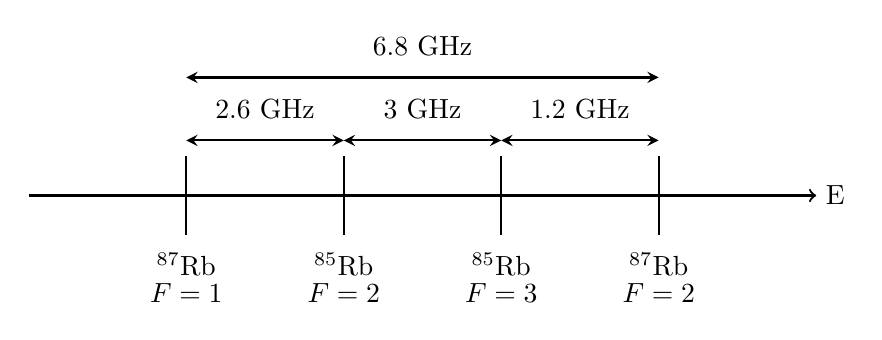
\begin{tikzpicture}
            % Energy levels
            \draw[thick] (2, 0.5) -- (2, -0.5);
            \draw[thick] (4, 0.5) -- (4, -0.5);
            \draw[thick] (6, 0.5) -- (6, -0.5);
            \draw[thick] (8, 0.5) -- (8, -0.5);
            
            % Labels for isotopes and F values
            \node[below] at (2, -0.6) {$^{87}$Rb};
            \node[below] at (4, -0.6) {$^{85}$Rb};
            \node[below] at (6, -0.6) {$^{85}$Rb};
            \node[below] at (8, -0.6) {$^{87}$Rb};
            
            \node[below] at (2, -1) {$F = 1$};
            \node[below] at (4, -1) {$F = 2$};
            \node[below] at (6, -1) {$F = 3$};
            \node[below] at (8, -1) {$F = 2$};
            
            % Arrows and frequencies
            \draw[<->, thick, >=stealth] (2, 1.5) -- (8, 1.5);
            \node[above] at (5, 1.65) {6.8 GHz};
            
            \draw[<->, thick, >=stealth] (2, 0.7) -- (4, 0.7);
            \node[above] at (3, 0.85) {2.6 GHz};
            
            \draw[<->, thick, >=stealth] (4, 0.7) -- (6, 0.7);
            \node[above] at (5, 0.85) {3 GHz};
            
            \draw[<->, thick, >=stealth] (6, 0.7) -- (8, 0.7);
            \node[above] at (7, 0.85) {1.2 GHz};
            
            % Energy axis
            \draw[->, thick] (0, 0) -- (10, 0);
            \node[right] at (10, 0) {E};
                
            \end{tikzpicture}
        \caption{ Theoretical frequency differences between peaks of the absorption spectrum. Calculated using [\ref{app:frequencies}]}
        \label{fig:absorption_frequencies}
    \end{subfigure}
    \caption{}
    \label{fig:absorption_peaks_frequencies}
\end{figure}

\pagebreak{}

The following table shows the comparison between the theoretical and experimental frequency differences between peaks:

\begin{table}[h]
    \centering
    \begin{tabular}{|c|cc|c|}
    \hline
    \multirow{2}{*}{Peaks} & \multicolumn{2}{c|}{Distance {[}GHz{]}} & \multirow{2}{*}{\% Error} \\ \cline{2-3}
                                            & \multicolumn{1}{c|}{Theoretical} & Experimental &       \\ \hline
    $^{87}\text{Rb}_1$ - $^{85}\text{Rb}_2$ & \multicolumn{1}{c|}{2.60}        & 2.65         & 1.9\% \\ \hline
    $^{85}\text{Rb}_2$ - $^{85}\text{Rb}_3$ & \multicolumn{1}{c|}{3.00}        & 2.87         & 4.3\% \\ \hline
    $^{85}\text{Rb}_3$ - $^{87}\text{Rb}_2$ & \multicolumn{1}{c|}{1.20}        & 1.10         & 8.3\%  \\ \hline
    $^{87}\text{Rb}_1$ - $^{87}\text{Rb}_2$ & \multicolumn{1}{c|}{6.80}        & 6.60         & 2.5\% \\ \hline
    \end{tabular}
    \caption{}
    \label{tab:frequency_differences}
\end{table}

All \% errors were within 10\%, with the highest error being 8.3\%, due to the distance itself being small; excarbating the error. In general, the errors are probably due to inaccuracies in the scale factor used, as an average of peak distances was used but the peak distances themselves can deviate alot.

Then, each peak was isolated and fitted with a Voigt profile, shown in the following plots:

\begin{figure}[h]
    \centering
    \begin{subfigure}{0.49\textwidth}
        \centering
        \scalebox{0.49}{%% Creator: Matplotlib, PGF backend
%%
%% To include the figure in your LaTeX document, write
%%   \input{<filename>.pgf}
%%
%% Make sure the required packages are loaded in your preamble
%%   \usepackage{pgf}
%%
%% Also ensure that all the required font packages are loaded; for instance,
%% the lmodern package is sometimes necessary when using math font.
%%   \usepackage{lmodern}
%%
%% Figures using additional raster images can only be included by \input if
%% they are in the same directory as the main LaTeX file. For loading figures
%% from other directories you can use the `import` package
%%   \usepackage{import}
%%
%% and then include the figures with
%%   \import{<path to file>}{<filename>.pgf}
%%
%% Matplotlib used the following preamble
%%   
%%   \usepackage{fontspec}
%%   \makeatletter\@ifpackageloaded{underscore}{}{\usepackage[strings]{underscore}}\makeatother
%%
\begingroup%
\makeatletter%
\begin{pgfpicture}%
\pgfpathrectangle{\pgfpointorigin}{\pgfqpoint{6.489553in}{4.010764in}}%
\pgfusepath{use as bounding box, clip}%
\begin{pgfscope}%
\pgfsetbuttcap%
\pgfsetmiterjoin%
\definecolor{currentfill}{rgb}{1.000000,1.000000,1.000000}%
\pgfsetfillcolor{currentfill}%
\pgfsetlinewidth{0.000000pt}%
\definecolor{currentstroke}{rgb}{1.000000,1.000000,1.000000}%
\pgfsetstrokecolor{currentstroke}%
\pgfsetdash{}{0pt}%
\pgfpathmoveto{\pgfqpoint{0.000000in}{0.000000in}}%
\pgfpathlineto{\pgfqpoint{6.489553in}{0.000000in}}%
\pgfpathlineto{\pgfqpoint{6.489553in}{4.010764in}}%
\pgfpathlineto{\pgfqpoint{0.000000in}{4.010764in}}%
\pgfpathlineto{\pgfqpoint{0.000000in}{0.000000in}}%
\pgfpathclose%
\pgfusepath{fill}%
\end{pgfscope}%
\begin{pgfscope}%
\pgfsetbuttcap%
\pgfsetmiterjoin%
\definecolor{currentfill}{rgb}{1.000000,1.000000,1.000000}%
\pgfsetfillcolor{currentfill}%
\pgfsetlinewidth{0.000000pt}%
\definecolor{currentstroke}{rgb}{0.000000,0.000000,0.000000}%
\pgfsetstrokecolor{currentstroke}%
\pgfsetstrokeopacity{0.000000}%
\pgfsetdash{}{0pt}%
\pgfpathmoveto{\pgfqpoint{0.811194in}{0.441184in}}%
\pgfpathlineto{\pgfqpoint{5.840598in}{0.441184in}}%
\pgfpathlineto{\pgfqpoint{5.840598in}{3.529473in}}%
\pgfpathlineto{\pgfqpoint{0.811194in}{3.529473in}}%
\pgfpathlineto{\pgfqpoint{0.811194in}{0.441184in}}%
\pgfpathclose%
\pgfusepath{fill}%
\end{pgfscope}%
\begin{pgfscope}%
\pgfpathrectangle{\pgfqpoint{0.811194in}{0.441184in}}{\pgfqpoint{5.029404in}{3.088289in}}%
\pgfusepath{clip}%
\pgfsetbuttcap%
\pgfsetroundjoin%
\definecolor{currentfill}{rgb}{0.000000,0.000000,1.000000}%
\pgfsetfillcolor{currentfill}%
\pgfsetlinewidth{1.003750pt}%
\definecolor{currentstroke}{rgb}{0.000000,0.000000,1.000000}%
\pgfsetstrokecolor{currentstroke}%
\pgfsetdash{}{0pt}%
\pgfsys@defobject{currentmarker}{\pgfqpoint{-0.018373in}{-0.018373in}}{\pgfqpoint{0.018373in}{0.018373in}}{%
\pgfpathmoveto{\pgfqpoint{0.000000in}{-0.018373in}}%
\pgfpathcurveto{\pgfqpoint{0.004873in}{-0.018373in}}{\pgfqpoint{0.009546in}{-0.016437in}}{\pgfqpoint{0.012992in}{-0.012992in}}%
\pgfpathcurveto{\pgfqpoint{0.016437in}{-0.009546in}}{\pgfqpoint{0.018373in}{-0.004873in}}{\pgfqpoint{0.018373in}{0.000000in}}%
\pgfpathcurveto{\pgfqpoint{0.018373in}{0.004873in}}{\pgfqpoint{0.016437in}{0.009546in}}{\pgfqpoint{0.012992in}{0.012992in}}%
\pgfpathcurveto{\pgfqpoint{0.009546in}{0.016437in}}{\pgfqpoint{0.004873in}{0.018373in}}{\pgfqpoint{0.000000in}{0.018373in}}%
\pgfpathcurveto{\pgfqpoint{-0.004873in}{0.018373in}}{\pgfqpoint{-0.009546in}{0.016437in}}{\pgfqpoint{-0.012992in}{0.012992in}}%
\pgfpathcurveto{\pgfqpoint{-0.016437in}{0.009546in}}{\pgfqpoint{-0.018373in}{0.004873in}}{\pgfqpoint{-0.018373in}{0.000000in}}%
\pgfpathcurveto{\pgfqpoint{-0.018373in}{-0.004873in}}{\pgfqpoint{-0.016437in}{-0.009546in}}{\pgfqpoint{-0.012992in}{-0.012992in}}%
\pgfpathcurveto{\pgfqpoint{-0.009546in}{-0.016437in}}{\pgfqpoint{-0.004873in}{-0.018373in}}{\pgfqpoint{0.000000in}{-0.018373in}}%
\pgfpathlineto{\pgfqpoint{0.000000in}{-0.018373in}}%
\pgfpathclose%
\pgfusepath{stroke,fill}%
}%
\begin{pgfscope}%
\pgfsys@transformshift{1.039803in}{0.685544in}%
\pgfsys@useobject{currentmarker}{}%
\end{pgfscope}%
\begin{pgfscope}%
\pgfsys@transformshift{1.122934in}{0.841518in}%
\pgfsys@useobject{currentmarker}{}%
\end{pgfscope}%
\begin{pgfscope}%
\pgfsys@transformshift{1.206065in}{1.101475in}%
\pgfsys@useobject{currentmarker}{}%
\end{pgfscope}%
\begin{pgfscope}%
\pgfsys@transformshift{1.289195in}{1.153466in}%
\pgfsys@useobject{currentmarker}{}%
\end{pgfscope}%
\begin{pgfscope}%
\pgfsys@transformshift{1.372326in}{1.569397in}%
\pgfsys@useobject{currentmarker}{}%
\end{pgfscope}%
\begin{pgfscope}%
\pgfsys@transformshift{1.455457in}{1.673380in}%
\pgfsys@useobject{currentmarker}{}%
\end{pgfscope}%
\begin{pgfscope}%
\pgfsys@transformshift{1.538587in}{1.881346in}%
\pgfsys@useobject{currentmarker}{}%
\end{pgfscope}%
\begin{pgfscope}%
\pgfsys@transformshift{1.621718in}{1.933337in}%
\pgfsys@useobject{currentmarker}{}%
\end{pgfscope}%
\begin{pgfscope}%
\pgfsys@transformshift{1.704848in}{2.297277in}%
\pgfsys@useobject{currentmarker}{}%
\end{pgfscope}%
\begin{pgfscope}%
\pgfsys@transformshift{1.787979in}{2.401259in}%
\pgfsys@useobject{currentmarker}{}%
\end{pgfscope}%
\begin{pgfscope}%
\pgfsys@transformshift{1.871110in}{2.557234in}%
\pgfsys@useobject{currentmarker}{}%
\end{pgfscope}%
\begin{pgfscope}%
\pgfsys@transformshift{1.954240in}{2.713208in}%
\pgfsys@useobject{currentmarker}{}%
\end{pgfscope}%
\begin{pgfscope}%
\pgfsys@transformshift{2.037371in}{2.921173in}%
\pgfsys@useobject{currentmarker}{}%
\end{pgfscope}%
\begin{pgfscope}%
\pgfsys@transformshift{2.120502in}{3.025156in}%
\pgfsys@useobject{currentmarker}{}%
\end{pgfscope}%
\begin{pgfscope}%
\pgfsys@transformshift{2.203632in}{3.077148in}%
\pgfsys@useobject{currentmarker}{}%
\end{pgfscope}%
\begin{pgfscope}%
\pgfsys@transformshift{2.286763in}{3.129139in}%
\pgfsys@useobject{currentmarker}{}%
\end{pgfscope}%
\begin{pgfscope}%
\pgfsys@transformshift{2.369894in}{3.181130in}%
\pgfsys@useobject{currentmarker}{}%
\end{pgfscope}%
\begin{pgfscope}%
\pgfsys@transformshift{2.453024in}{3.285113in}%
\pgfsys@useobject{currentmarker}{}%
\end{pgfscope}%
\begin{pgfscope}%
\pgfsys@transformshift{2.536155in}{3.233122in}%
\pgfsys@useobject{currentmarker}{}%
\end{pgfscope}%
\begin{pgfscope}%
\pgfsys@transformshift{2.619286in}{3.337104in}%
\pgfsys@useobject{currentmarker}{}%
\end{pgfscope}%
\begin{pgfscope}%
\pgfsys@transformshift{2.702416in}{3.389096in}%
\pgfsys@useobject{currentmarker}{}%
\end{pgfscope}%
\begin{pgfscope}%
\pgfsys@transformshift{2.785547in}{3.181130in}%
\pgfsys@useobject{currentmarker}{}%
\end{pgfscope}%
\begin{pgfscope}%
\pgfsys@transformshift{2.868677in}{3.077148in}%
\pgfsys@useobject{currentmarker}{}%
\end{pgfscope}%
\begin{pgfscope}%
\pgfsys@transformshift{2.951808in}{3.025156in}%
\pgfsys@useobject{currentmarker}{}%
\end{pgfscope}%
\begin{pgfscope}%
\pgfsys@transformshift{3.034939in}{2.921173in}%
\pgfsys@useobject{currentmarker}{}%
\end{pgfscope}%
\begin{pgfscope}%
\pgfsys@transformshift{3.118069in}{2.661216in}%
\pgfsys@useobject{currentmarker}{}%
\end{pgfscope}%
\begin{pgfscope}%
\pgfsys@transformshift{3.201200in}{2.505242in}%
\pgfsys@useobject{currentmarker}{}%
\end{pgfscope}%
\begin{pgfscope}%
\pgfsys@transformshift{3.284331in}{2.401259in}%
\pgfsys@useobject{currentmarker}{}%
\end{pgfscope}%
\begin{pgfscope}%
\pgfsys@transformshift{3.367461in}{2.401259in}%
\pgfsys@useobject{currentmarker}{}%
\end{pgfscope}%
\begin{pgfscope}%
\pgfsys@transformshift{3.450592in}{1.881346in}%
\pgfsys@useobject{currentmarker}{}%
\end{pgfscope}%
\begin{pgfscope}%
\pgfsys@transformshift{3.533723in}{1.777363in}%
\pgfsys@useobject{currentmarker}{}%
\end{pgfscope}%
\begin{pgfscope}%
\pgfsys@transformshift{3.616853in}{1.829354in}%
\pgfsys@useobject{currentmarker}{}%
\end{pgfscope}%
\begin{pgfscope}%
\pgfsys@transformshift{3.699984in}{1.569397in}%
\pgfsys@useobject{currentmarker}{}%
\end{pgfscope}%
\begin{pgfscope}%
\pgfsys@transformshift{3.783114in}{1.309440in}%
\pgfsys@useobject{currentmarker}{}%
\end{pgfscope}%
\begin{pgfscope}%
\pgfsys@transformshift{3.866245in}{1.361432in}%
\pgfsys@useobject{currentmarker}{}%
\end{pgfscope}%
\begin{pgfscope}%
\pgfsys@transformshift{3.949376in}{1.101475in}%
\pgfsys@useobject{currentmarker}{}%
\end{pgfscope}%
\begin{pgfscope}%
\pgfsys@transformshift{4.032506in}{1.153466in}%
\pgfsys@useobject{currentmarker}{}%
\end{pgfscope}%
\begin{pgfscope}%
\pgfsys@transformshift{4.115637in}{0.893509in}%
\pgfsys@useobject{currentmarker}{}%
\end{pgfscope}%
\begin{pgfscope}%
\pgfsys@transformshift{4.198768in}{0.893509in}%
\pgfsys@useobject{currentmarker}{}%
\end{pgfscope}%
\begin{pgfscope}%
\pgfsys@transformshift{4.281898in}{0.997492in}%
\pgfsys@useobject{currentmarker}{}%
\end{pgfscope}%
\begin{pgfscope}%
\pgfsys@transformshift{4.365029in}{0.945501in}%
\pgfsys@useobject{currentmarker}{}%
\end{pgfscope}%
\begin{pgfscope}%
\pgfsys@transformshift{4.448160in}{0.893509in}%
\pgfsys@useobject{currentmarker}{}%
\end{pgfscope}%
\begin{pgfscope}%
\pgfsys@transformshift{4.531290in}{0.841518in}%
\pgfsys@useobject{currentmarker}{}%
\end{pgfscope}%
\begin{pgfscope}%
\pgfsys@transformshift{4.614421in}{0.737535in}%
\pgfsys@useobject{currentmarker}{}%
\end{pgfscope}%
\begin{pgfscope}%
\pgfsys@transformshift{4.697551in}{0.737535in}%
\pgfsys@useobject{currentmarker}{}%
\end{pgfscope}%
\begin{pgfscope}%
\pgfsys@transformshift{4.780682in}{0.581561in}%
\pgfsys@useobject{currentmarker}{}%
\end{pgfscope}%
\begin{pgfscope}%
\pgfsys@transformshift{4.863813in}{0.685544in}%
\pgfsys@useobject{currentmarker}{}%
\end{pgfscope}%
\begin{pgfscope}%
\pgfsys@transformshift{4.946943in}{0.633552in}%
\pgfsys@useobject{currentmarker}{}%
\end{pgfscope}%
\begin{pgfscope}%
\pgfsys@transformshift{5.030074in}{0.685544in}%
\pgfsys@useobject{currentmarker}{}%
\end{pgfscope}%
\begin{pgfscope}%
\pgfsys@transformshift{5.113205in}{0.893509in}%
\pgfsys@useobject{currentmarker}{}%
\end{pgfscope}%
\begin{pgfscope}%
\pgfsys@transformshift{5.196335in}{0.945501in}%
\pgfsys@useobject{currentmarker}{}%
\end{pgfscope}%
\begin{pgfscope}%
\pgfsys@transformshift{5.279466in}{0.945501in}%
\pgfsys@useobject{currentmarker}{}%
\end{pgfscope}%
\begin{pgfscope}%
\pgfsys@transformshift{5.362597in}{0.685544in}%
\pgfsys@useobject{currentmarker}{}%
\end{pgfscope}%
\begin{pgfscope}%
\pgfsys@transformshift{5.445727in}{0.997492in}%
\pgfsys@useobject{currentmarker}{}%
\end{pgfscope}%
\begin{pgfscope}%
\pgfsys@transformshift{5.528858in}{0.893509in}%
\pgfsys@useobject{currentmarker}{}%
\end{pgfscope}%
\begin{pgfscope}%
\pgfsys@transformshift{5.611989in}{1.049483in}%
\pgfsys@useobject{currentmarker}{}%
\end{pgfscope}%
\end{pgfscope}%
\begin{pgfscope}%
\pgfsetbuttcap%
\pgfsetroundjoin%
\definecolor{currentfill}{rgb}{0.000000,0.000000,0.000000}%
\pgfsetfillcolor{currentfill}%
\pgfsetlinewidth{0.803000pt}%
\definecolor{currentstroke}{rgb}{0.000000,0.000000,0.000000}%
\pgfsetstrokecolor{currentstroke}%
\pgfsetdash{}{0pt}%
\pgfsys@defobject{currentmarker}{\pgfqpoint{0.000000in}{-0.048611in}}{\pgfqpoint{0.000000in}{0.000000in}}{%
\pgfpathmoveto{\pgfqpoint{0.000000in}{0.000000in}}%
\pgfpathlineto{\pgfqpoint{0.000000in}{-0.048611in}}%
\pgfusepath{stroke,fill}%
}%
\begin{pgfscope}%
\pgfsys@transformshift{1.299171in}{0.441184in}%
\pgfsys@useobject{currentmarker}{}%
\end{pgfscope}%
\end{pgfscope}%
\begin{pgfscope}%
\definecolor{textcolor}{rgb}{0.000000,0.000000,0.000000}%
\pgfsetstrokecolor{textcolor}%
\pgfsetfillcolor{textcolor}%
\pgftext[x=1.299171in,y=0.343962in,,top]{\color{textcolor}\rmfamily\fontsize{10.000000}{12.000000}\selectfont \(\displaystyle {2.6}\)}%
\end{pgfscope}%
\begin{pgfscope}%
\pgfsetbuttcap%
\pgfsetroundjoin%
\definecolor{currentfill}{rgb}{0.000000,0.000000,0.000000}%
\pgfsetfillcolor{currentfill}%
\pgfsetlinewidth{0.803000pt}%
\definecolor{currentstroke}{rgb}{0.000000,0.000000,0.000000}%
\pgfsetstrokecolor{currentstroke}%
\pgfsetdash{}{0pt}%
\pgfsys@defobject{currentmarker}{\pgfqpoint{0.000000in}{-0.048611in}}{\pgfqpoint{0.000000in}{0.000000in}}{%
\pgfpathmoveto{\pgfqpoint{0.000000in}{0.000000in}}%
\pgfpathlineto{\pgfqpoint{0.000000in}{-0.048611in}}%
\pgfusepath{stroke,fill}%
}%
\begin{pgfscope}%
\pgfsys@transformshift{1.901037in}{0.441184in}%
\pgfsys@useobject{currentmarker}{}%
\end{pgfscope}%
\end{pgfscope}%
\begin{pgfscope}%
\definecolor{textcolor}{rgb}{0.000000,0.000000,0.000000}%
\pgfsetstrokecolor{textcolor}%
\pgfsetfillcolor{textcolor}%
\pgftext[x=1.901037in,y=0.343962in,,top]{\color{textcolor}\rmfamily\fontsize{10.000000}{12.000000}\selectfont \(\displaystyle {2.8}\)}%
\end{pgfscope}%
\begin{pgfscope}%
\pgfsetbuttcap%
\pgfsetroundjoin%
\definecolor{currentfill}{rgb}{0.000000,0.000000,0.000000}%
\pgfsetfillcolor{currentfill}%
\pgfsetlinewidth{0.803000pt}%
\definecolor{currentstroke}{rgb}{0.000000,0.000000,0.000000}%
\pgfsetstrokecolor{currentstroke}%
\pgfsetdash{}{0pt}%
\pgfsys@defobject{currentmarker}{\pgfqpoint{0.000000in}{-0.048611in}}{\pgfqpoint{0.000000in}{0.000000in}}{%
\pgfpathmoveto{\pgfqpoint{0.000000in}{0.000000in}}%
\pgfpathlineto{\pgfqpoint{0.000000in}{-0.048611in}}%
\pgfusepath{stroke,fill}%
}%
\begin{pgfscope}%
\pgfsys@transformshift{2.502903in}{0.441184in}%
\pgfsys@useobject{currentmarker}{}%
\end{pgfscope}%
\end{pgfscope}%
\begin{pgfscope}%
\definecolor{textcolor}{rgb}{0.000000,0.000000,0.000000}%
\pgfsetstrokecolor{textcolor}%
\pgfsetfillcolor{textcolor}%
\pgftext[x=2.502903in,y=0.343962in,,top]{\color{textcolor}\rmfamily\fontsize{10.000000}{12.000000}\selectfont \(\displaystyle {3.0}\)}%
\end{pgfscope}%
\begin{pgfscope}%
\pgfsetbuttcap%
\pgfsetroundjoin%
\definecolor{currentfill}{rgb}{0.000000,0.000000,0.000000}%
\pgfsetfillcolor{currentfill}%
\pgfsetlinewidth{0.803000pt}%
\definecolor{currentstroke}{rgb}{0.000000,0.000000,0.000000}%
\pgfsetstrokecolor{currentstroke}%
\pgfsetdash{}{0pt}%
\pgfsys@defobject{currentmarker}{\pgfqpoint{0.000000in}{-0.048611in}}{\pgfqpoint{0.000000in}{0.000000in}}{%
\pgfpathmoveto{\pgfqpoint{0.000000in}{0.000000in}}%
\pgfpathlineto{\pgfqpoint{0.000000in}{-0.048611in}}%
\pgfusepath{stroke,fill}%
}%
\begin{pgfscope}%
\pgfsys@transformshift{3.104768in}{0.441184in}%
\pgfsys@useobject{currentmarker}{}%
\end{pgfscope}%
\end{pgfscope}%
\begin{pgfscope}%
\definecolor{textcolor}{rgb}{0.000000,0.000000,0.000000}%
\pgfsetstrokecolor{textcolor}%
\pgfsetfillcolor{textcolor}%
\pgftext[x=3.104768in,y=0.343962in,,top]{\color{textcolor}\rmfamily\fontsize{10.000000}{12.000000}\selectfont \(\displaystyle {3.2}\)}%
\end{pgfscope}%
\begin{pgfscope}%
\pgfsetbuttcap%
\pgfsetroundjoin%
\definecolor{currentfill}{rgb}{0.000000,0.000000,0.000000}%
\pgfsetfillcolor{currentfill}%
\pgfsetlinewidth{0.803000pt}%
\definecolor{currentstroke}{rgb}{0.000000,0.000000,0.000000}%
\pgfsetstrokecolor{currentstroke}%
\pgfsetdash{}{0pt}%
\pgfsys@defobject{currentmarker}{\pgfqpoint{0.000000in}{-0.048611in}}{\pgfqpoint{0.000000in}{0.000000in}}{%
\pgfpathmoveto{\pgfqpoint{0.000000in}{0.000000in}}%
\pgfpathlineto{\pgfqpoint{0.000000in}{-0.048611in}}%
\pgfusepath{stroke,fill}%
}%
\begin{pgfscope}%
\pgfsys@transformshift{3.706634in}{0.441184in}%
\pgfsys@useobject{currentmarker}{}%
\end{pgfscope}%
\end{pgfscope}%
\begin{pgfscope}%
\definecolor{textcolor}{rgb}{0.000000,0.000000,0.000000}%
\pgfsetstrokecolor{textcolor}%
\pgfsetfillcolor{textcolor}%
\pgftext[x=3.706634in,y=0.343962in,,top]{\color{textcolor}\rmfamily\fontsize{10.000000}{12.000000}\selectfont \(\displaystyle {3.4}\)}%
\end{pgfscope}%
\begin{pgfscope}%
\pgfsetbuttcap%
\pgfsetroundjoin%
\definecolor{currentfill}{rgb}{0.000000,0.000000,0.000000}%
\pgfsetfillcolor{currentfill}%
\pgfsetlinewidth{0.803000pt}%
\definecolor{currentstroke}{rgb}{0.000000,0.000000,0.000000}%
\pgfsetstrokecolor{currentstroke}%
\pgfsetdash{}{0pt}%
\pgfsys@defobject{currentmarker}{\pgfqpoint{0.000000in}{-0.048611in}}{\pgfqpoint{0.000000in}{0.000000in}}{%
\pgfpathmoveto{\pgfqpoint{0.000000in}{0.000000in}}%
\pgfpathlineto{\pgfqpoint{0.000000in}{-0.048611in}}%
\pgfusepath{stroke,fill}%
}%
\begin{pgfscope}%
\pgfsys@transformshift{4.308500in}{0.441184in}%
\pgfsys@useobject{currentmarker}{}%
\end{pgfscope}%
\end{pgfscope}%
\begin{pgfscope}%
\definecolor{textcolor}{rgb}{0.000000,0.000000,0.000000}%
\pgfsetstrokecolor{textcolor}%
\pgfsetfillcolor{textcolor}%
\pgftext[x=4.308500in,y=0.343962in,,top]{\color{textcolor}\rmfamily\fontsize{10.000000}{12.000000}\selectfont \(\displaystyle {3.6}\)}%
\end{pgfscope}%
\begin{pgfscope}%
\pgfsetbuttcap%
\pgfsetroundjoin%
\definecolor{currentfill}{rgb}{0.000000,0.000000,0.000000}%
\pgfsetfillcolor{currentfill}%
\pgfsetlinewidth{0.803000pt}%
\definecolor{currentstroke}{rgb}{0.000000,0.000000,0.000000}%
\pgfsetstrokecolor{currentstroke}%
\pgfsetdash{}{0pt}%
\pgfsys@defobject{currentmarker}{\pgfqpoint{0.000000in}{-0.048611in}}{\pgfqpoint{0.000000in}{0.000000in}}{%
\pgfpathmoveto{\pgfqpoint{0.000000in}{0.000000in}}%
\pgfpathlineto{\pgfqpoint{0.000000in}{-0.048611in}}%
\pgfusepath{stroke,fill}%
}%
\begin{pgfscope}%
\pgfsys@transformshift{4.910366in}{0.441184in}%
\pgfsys@useobject{currentmarker}{}%
\end{pgfscope}%
\end{pgfscope}%
\begin{pgfscope}%
\definecolor{textcolor}{rgb}{0.000000,0.000000,0.000000}%
\pgfsetstrokecolor{textcolor}%
\pgfsetfillcolor{textcolor}%
\pgftext[x=4.910366in,y=0.343962in,,top]{\color{textcolor}\rmfamily\fontsize{10.000000}{12.000000}\selectfont \(\displaystyle {3.8}\)}%
\end{pgfscope}%
\begin{pgfscope}%
\pgfsetbuttcap%
\pgfsetroundjoin%
\definecolor{currentfill}{rgb}{0.000000,0.000000,0.000000}%
\pgfsetfillcolor{currentfill}%
\pgfsetlinewidth{0.803000pt}%
\definecolor{currentstroke}{rgb}{0.000000,0.000000,0.000000}%
\pgfsetstrokecolor{currentstroke}%
\pgfsetdash{}{0pt}%
\pgfsys@defobject{currentmarker}{\pgfqpoint{0.000000in}{-0.048611in}}{\pgfqpoint{0.000000in}{0.000000in}}{%
\pgfpathmoveto{\pgfqpoint{0.000000in}{0.000000in}}%
\pgfpathlineto{\pgfqpoint{0.000000in}{-0.048611in}}%
\pgfusepath{stroke,fill}%
}%
\begin{pgfscope}%
\pgfsys@transformshift{5.512232in}{0.441184in}%
\pgfsys@useobject{currentmarker}{}%
\end{pgfscope}%
\end{pgfscope}%
\begin{pgfscope}%
\definecolor{textcolor}{rgb}{0.000000,0.000000,0.000000}%
\pgfsetstrokecolor{textcolor}%
\pgfsetfillcolor{textcolor}%
\pgftext[x=5.512232in,y=0.343962in,,top]{\color{textcolor}\rmfamily\fontsize{10.000000}{12.000000}\selectfont \(\displaystyle {4.0}\)}%
\end{pgfscope}%
\begin{pgfscope}%
\definecolor{textcolor}{rgb}{0.000000,0.000000,0.000000}%
\pgfsetstrokecolor{textcolor}%
\pgfsetfillcolor{textcolor}%
\pgftext[x=3.325896in,y=0.165073in,,top]{\color{textcolor}\rmfamily\fontsize{10.000000}{12.000000}\selectfont Frequency [GHz]}%
\end{pgfscope}%
\begin{pgfscope}%
\pgfsetbuttcap%
\pgfsetroundjoin%
\definecolor{currentfill}{rgb}{0.000000,0.000000,0.000000}%
\pgfsetfillcolor{currentfill}%
\pgfsetlinewidth{0.803000pt}%
\definecolor{currentstroke}{rgb}{0.000000,0.000000,0.000000}%
\pgfsetstrokecolor{currentstroke}%
\pgfsetdash{}{0pt}%
\pgfsys@defobject{currentmarker}{\pgfqpoint{-0.048611in}{0.000000in}}{\pgfqpoint{-0.000000in}{0.000000in}}{%
\pgfpathmoveto{\pgfqpoint{-0.000000in}{0.000000in}}%
\pgfpathlineto{\pgfqpoint{-0.048611in}{0.000000in}}%
\pgfusepath{stroke,fill}%
}%
\begin{pgfscope}%
\pgfsys@transformshift{0.811194in}{0.945501in}%
\pgfsys@useobject{currentmarker}{}%
\end{pgfscope}%
\end{pgfscope}%
\begin{pgfscope}%
\definecolor{textcolor}{rgb}{0.000000,0.000000,0.000000}%
\pgfsetstrokecolor{textcolor}%
\pgfsetfillcolor{textcolor}%
\pgftext[x=0.536502in, y=0.897306in, left, base]{\color{textcolor}\rmfamily\fontsize{10.000000}{12.000000}\selectfont \(\displaystyle {0.6}\)}%
\end{pgfscope}%
\begin{pgfscope}%
\pgfsetbuttcap%
\pgfsetroundjoin%
\definecolor{currentfill}{rgb}{0.000000,0.000000,0.000000}%
\pgfsetfillcolor{currentfill}%
\pgfsetlinewidth{0.803000pt}%
\definecolor{currentstroke}{rgb}{0.000000,0.000000,0.000000}%
\pgfsetstrokecolor{currentstroke}%
\pgfsetdash{}{0pt}%
\pgfsys@defobject{currentmarker}{\pgfqpoint{-0.048611in}{0.000000in}}{\pgfqpoint{-0.000000in}{0.000000in}}{%
\pgfpathmoveto{\pgfqpoint{-0.000000in}{0.000000in}}%
\pgfpathlineto{\pgfqpoint{-0.048611in}{0.000000in}}%
\pgfusepath{stroke,fill}%
}%
\begin{pgfscope}%
\pgfsys@transformshift{0.811194in}{1.465414in}%
\pgfsys@useobject{currentmarker}{}%
\end{pgfscope}%
\end{pgfscope}%
\begin{pgfscope}%
\definecolor{textcolor}{rgb}{0.000000,0.000000,0.000000}%
\pgfsetstrokecolor{textcolor}%
\pgfsetfillcolor{textcolor}%
\pgftext[x=0.536502in, y=1.417220in, left, base]{\color{textcolor}\rmfamily\fontsize{10.000000}{12.000000}\selectfont \(\displaystyle {0.8}\)}%
\end{pgfscope}%
\begin{pgfscope}%
\pgfsetbuttcap%
\pgfsetroundjoin%
\definecolor{currentfill}{rgb}{0.000000,0.000000,0.000000}%
\pgfsetfillcolor{currentfill}%
\pgfsetlinewidth{0.803000pt}%
\definecolor{currentstroke}{rgb}{0.000000,0.000000,0.000000}%
\pgfsetstrokecolor{currentstroke}%
\pgfsetdash{}{0pt}%
\pgfsys@defobject{currentmarker}{\pgfqpoint{-0.048611in}{0.000000in}}{\pgfqpoint{-0.000000in}{0.000000in}}{%
\pgfpathmoveto{\pgfqpoint{-0.000000in}{0.000000in}}%
\pgfpathlineto{\pgfqpoint{-0.048611in}{0.000000in}}%
\pgfusepath{stroke,fill}%
}%
\begin{pgfscope}%
\pgfsys@transformshift{0.811194in}{1.985328in}%
\pgfsys@useobject{currentmarker}{}%
\end{pgfscope}%
\end{pgfscope}%
\begin{pgfscope}%
\definecolor{textcolor}{rgb}{0.000000,0.000000,0.000000}%
\pgfsetstrokecolor{textcolor}%
\pgfsetfillcolor{textcolor}%
\pgftext[x=0.536502in, y=1.937134in, left, base]{\color{textcolor}\rmfamily\fontsize{10.000000}{12.000000}\selectfont \(\displaystyle {1.0}\)}%
\end{pgfscope}%
\begin{pgfscope}%
\pgfsetbuttcap%
\pgfsetroundjoin%
\definecolor{currentfill}{rgb}{0.000000,0.000000,0.000000}%
\pgfsetfillcolor{currentfill}%
\pgfsetlinewidth{0.803000pt}%
\definecolor{currentstroke}{rgb}{0.000000,0.000000,0.000000}%
\pgfsetstrokecolor{currentstroke}%
\pgfsetdash{}{0pt}%
\pgfsys@defobject{currentmarker}{\pgfqpoint{-0.048611in}{0.000000in}}{\pgfqpoint{-0.000000in}{0.000000in}}{%
\pgfpathmoveto{\pgfqpoint{-0.000000in}{0.000000in}}%
\pgfpathlineto{\pgfqpoint{-0.048611in}{0.000000in}}%
\pgfusepath{stroke,fill}%
}%
\begin{pgfscope}%
\pgfsys@transformshift{0.811194in}{2.505242in}%
\pgfsys@useobject{currentmarker}{}%
\end{pgfscope}%
\end{pgfscope}%
\begin{pgfscope}%
\definecolor{textcolor}{rgb}{0.000000,0.000000,0.000000}%
\pgfsetstrokecolor{textcolor}%
\pgfsetfillcolor{textcolor}%
\pgftext[x=0.536502in, y=2.457048in, left, base]{\color{textcolor}\rmfamily\fontsize{10.000000}{12.000000}\selectfont \(\displaystyle {1.2}\)}%
\end{pgfscope}%
\begin{pgfscope}%
\pgfsetbuttcap%
\pgfsetroundjoin%
\definecolor{currentfill}{rgb}{0.000000,0.000000,0.000000}%
\pgfsetfillcolor{currentfill}%
\pgfsetlinewidth{0.803000pt}%
\definecolor{currentstroke}{rgb}{0.000000,0.000000,0.000000}%
\pgfsetstrokecolor{currentstroke}%
\pgfsetdash{}{0pt}%
\pgfsys@defobject{currentmarker}{\pgfqpoint{-0.048611in}{0.000000in}}{\pgfqpoint{-0.000000in}{0.000000in}}{%
\pgfpathmoveto{\pgfqpoint{-0.000000in}{0.000000in}}%
\pgfpathlineto{\pgfqpoint{-0.048611in}{0.000000in}}%
\pgfusepath{stroke,fill}%
}%
\begin{pgfscope}%
\pgfsys@transformshift{0.811194in}{3.025156in}%
\pgfsys@useobject{currentmarker}{}%
\end{pgfscope}%
\end{pgfscope}%
\begin{pgfscope}%
\definecolor{textcolor}{rgb}{0.000000,0.000000,0.000000}%
\pgfsetstrokecolor{textcolor}%
\pgfsetfillcolor{textcolor}%
\pgftext[x=0.536502in, y=2.976962in, left, base]{\color{textcolor}\rmfamily\fontsize{10.000000}{12.000000}\selectfont \(\displaystyle {1.4}\)}%
\end{pgfscope}%
\begin{pgfscope}%
\definecolor{textcolor}{rgb}{0.000000,0.000000,0.000000}%
\pgfsetstrokecolor{textcolor}%
\pgfsetfillcolor{textcolor}%
\pgftext[x=0.480947in,y=1.985328in,,bottom,rotate=90.000000]{\color{textcolor}\rmfamily\fontsize{10.000000}{12.000000}\selectfont Intensity [a.u.]}%
\end{pgfscope}%
\begin{pgfscope}%
\pgfpathrectangle{\pgfqpoint{0.811194in}{0.441184in}}{\pgfqpoint{5.029404in}{3.088289in}}%
\pgfusepath{clip}%
\pgfsetrectcap%
\pgfsetroundjoin%
\pgfsetlinewidth{1.505625pt}%
\definecolor{currentstroke}{rgb}{0.000000,0.501961,0.000000}%
\pgfsetstrokecolor{currentstroke}%
\pgfsetdash{}{0pt}%
\pgfpathmoveto{\pgfqpoint{1.039803in}{1.076085in}}%
\pgfpathlineto{\pgfqpoint{1.122934in}{1.155816in}}%
\pgfpathlineto{\pgfqpoint{1.206065in}{1.249601in}}%
\pgfpathlineto{\pgfqpoint{1.289195in}{1.358118in}}%
\pgfpathlineto{\pgfqpoint{1.372326in}{1.481572in}}%
\pgfpathlineto{\pgfqpoint{1.455457in}{1.619581in}}%
\pgfpathlineto{\pgfqpoint{1.538587in}{1.771076in}}%
\pgfpathlineto{\pgfqpoint{1.621718in}{1.934228in}}%
\pgfpathlineto{\pgfqpoint{1.704848in}{2.106418in}}%
\pgfpathlineto{\pgfqpoint{1.787979in}{2.284247in}}%
\pgfpathlineto{\pgfqpoint{1.871110in}{2.463617in}}%
\pgfpathlineto{\pgfqpoint{1.954240in}{2.639852in}}%
\pgfpathlineto{\pgfqpoint{2.037371in}{2.807889in}}%
\pgfpathlineto{\pgfqpoint{2.120502in}{2.962506in}}%
\pgfpathlineto{\pgfqpoint{2.203632in}{3.098586in}}%
\pgfpathlineto{\pgfqpoint{2.286763in}{3.211394in}}%
\pgfpathlineto{\pgfqpoint{2.369894in}{3.296853in}}%
\pgfpathlineto{\pgfqpoint{2.453024in}{3.351786in}}%
\pgfpathlineto{\pgfqpoint{2.536155in}{3.374110in}}%
\pgfpathlineto{\pgfqpoint{2.619286in}{3.362971in}}%
\pgfpathlineto{\pgfqpoint{2.702416in}{3.318797in}}%
\pgfpathlineto{\pgfqpoint{2.785547in}{3.243268in}}%
\pgfpathlineto{\pgfqpoint{2.868677in}{3.139213in}}%
\pgfpathlineto{\pgfqpoint{2.951808in}{3.010434in}}%
\pgfpathlineto{\pgfqpoint{3.034939in}{2.861474in}}%
\pgfpathlineto{\pgfqpoint{3.118069in}{2.697353in}}%
\pgfpathlineto{\pgfqpoint{3.201200in}{2.523289in}}%
\pgfpathlineto{\pgfqpoint{3.284331in}{2.344426in}}%
\pgfpathlineto{\pgfqpoint{3.367461in}{2.165591in}}%
\pgfpathlineto{\pgfqpoint{3.450592in}{1.991096in}}%
\pgfpathlineto{\pgfqpoint{3.533723in}{1.824583in}}%
\pgfpathlineto{\pgfqpoint{3.616853in}{1.668937in}}%
\pgfpathlineto{\pgfqpoint{3.699984in}{1.526252in}}%
\pgfpathlineto{\pgfqpoint{3.783114in}{1.397844in}}%
\pgfpathlineto{\pgfqpoint{3.866245in}{1.284316in}}%
\pgfpathlineto{\pgfqpoint{3.949376in}{1.185647in}}%
\pgfpathlineto{\pgfqpoint{4.032506in}{1.101304in}}%
\pgfpathlineto{\pgfqpoint{4.115637in}{1.030365in}}%
\pgfpathlineto{\pgfqpoint{4.198768in}{0.971637in}}%
\pgfpathlineto{\pgfqpoint{4.281898in}{0.923767in}}%
\pgfpathlineto{\pgfqpoint{4.365029in}{0.885339in}}%
\pgfpathlineto{\pgfqpoint{4.448160in}{0.854951in}}%
\pgfpathlineto{\pgfqpoint{4.531290in}{0.831276in}}%
\pgfpathlineto{\pgfqpoint{4.614421in}{0.813100in}}%
\pgfpathlineto{\pgfqpoint{4.697551in}{0.799346in}}%
\pgfpathlineto{\pgfqpoint{4.780682in}{0.789089in}}%
\pgfpathlineto{\pgfqpoint{4.863813in}{0.781547in}}%
\pgfpathlineto{\pgfqpoint{4.946943in}{0.776080in}}%
\pgfpathlineto{\pgfqpoint{5.030074in}{0.772172in}}%
\pgfpathlineto{\pgfqpoint{5.113205in}{0.769418in}}%
\pgfpathlineto{\pgfqpoint{5.196335in}{0.767504in}}%
\pgfpathlineto{\pgfqpoint{5.279466in}{0.766192in}}%
\pgfpathlineto{\pgfqpoint{5.362597in}{0.765305in}}%
\pgfpathlineto{\pgfqpoint{5.445727in}{0.764713in}}%
\pgfpathlineto{\pgfqpoint{5.528858in}{0.764324in}}%
\pgfpathlineto{\pgfqpoint{5.611989in}{0.764072in}}%
\pgfusepath{stroke}%
\end{pgfscope}%
\begin{pgfscope}%
\pgfsetrectcap%
\pgfsetmiterjoin%
\pgfsetlinewidth{0.803000pt}%
\definecolor{currentstroke}{rgb}{0.000000,0.000000,0.000000}%
\pgfsetstrokecolor{currentstroke}%
\pgfsetdash{}{0pt}%
\pgfpathmoveto{\pgfqpoint{0.811194in}{0.441184in}}%
\pgfpathlineto{\pgfqpoint{0.811194in}{3.529473in}}%
\pgfusepath{stroke}%
\end{pgfscope}%
\begin{pgfscope}%
\pgfsetrectcap%
\pgfsetmiterjoin%
\pgfsetlinewidth{0.803000pt}%
\definecolor{currentstroke}{rgb}{0.000000,0.000000,0.000000}%
\pgfsetstrokecolor{currentstroke}%
\pgfsetdash{}{0pt}%
\pgfpathmoveto{\pgfqpoint{5.840598in}{0.441184in}}%
\pgfpathlineto{\pgfqpoint{5.840598in}{3.529473in}}%
\pgfusepath{stroke}%
\end{pgfscope}%
\begin{pgfscope}%
\pgfsetrectcap%
\pgfsetmiterjoin%
\pgfsetlinewidth{0.803000pt}%
\definecolor{currentstroke}{rgb}{0.000000,0.000000,0.000000}%
\pgfsetstrokecolor{currentstroke}%
\pgfsetdash{}{0pt}%
\pgfpathmoveto{\pgfqpoint{0.811194in}{0.441184in}}%
\pgfpathlineto{\pgfqpoint{5.840598in}{0.441184in}}%
\pgfusepath{stroke}%
\end{pgfscope}%
\begin{pgfscope}%
\pgfsetrectcap%
\pgfsetmiterjoin%
\pgfsetlinewidth{0.803000pt}%
\definecolor{currentstroke}{rgb}{0.000000,0.000000,0.000000}%
\pgfsetstrokecolor{currentstroke}%
\pgfsetdash{}{0pt}%
\pgfpathmoveto{\pgfqpoint{0.811194in}{3.529473in}}%
\pgfpathlineto{\pgfqpoint{5.840598in}{3.529473in}}%
\pgfusepath{stroke}%
\end{pgfscope}%
\begin{pgfscope}%
\definecolor{textcolor}{rgb}{0.000000,0.000000,0.000000}%
\pgfsetstrokecolor{textcolor}%
\pgfsetfillcolor{textcolor}%
\pgftext[x=3.325896in,y=3.612806in,,base]{\color{textcolor}\rmfamily\fontsize{12.000000}{14.400000}\selectfont Peak 1}%
\end{pgfscope}%
\begin{pgfscope}%
\pgfsetbuttcap%
\pgfsetmiterjoin%
\definecolor{currentfill}{rgb}{1.000000,1.000000,1.000000}%
\pgfsetfillcolor{currentfill}%
\pgfsetfillopacity{0.800000}%
\pgfsetlinewidth{1.003750pt}%
\definecolor{currentstroke}{rgb}{0.800000,0.800000,0.800000}%
\pgfsetstrokecolor{currentstroke}%
\pgfsetstrokeopacity{0.800000}%
\pgfsetdash{}{0pt}%
\pgfpathmoveto{\pgfqpoint{3.846895in}{2.858605in}}%
\pgfpathlineto{\pgfqpoint{5.743376in}{2.858605in}}%
\pgfpathquadraticcurveto{\pgfqpoint{5.771153in}{2.858605in}}{\pgfqpoint{5.771153in}{2.886383in}}%
\pgfpathlineto{\pgfqpoint{5.771153in}{3.432250in}}%
\pgfpathquadraticcurveto{\pgfqpoint{5.771153in}{3.460028in}}{\pgfqpoint{5.743376in}{3.460028in}}%
\pgfpathlineto{\pgfqpoint{3.846895in}{3.460028in}}%
\pgfpathquadraticcurveto{\pgfqpoint{3.819117in}{3.460028in}}{\pgfqpoint{3.819117in}{3.432250in}}%
\pgfpathlineto{\pgfqpoint{3.819117in}{2.886383in}}%
\pgfpathquadraticcurveto{\pgfqpoint{3.819117in}{2.858605in}}{\pgfqpoint{3.846895in}{2.858605in}}%
\pgfpathlineto{\pgfqpoint{3.846895in}{2.858605in}}%
\pgfpathclose%
\pgfusepath{stroke,fill}%
\end{pgfscope}%
\begin{pgfscope}%
\pgfsetbuttcap%
\pgfsetroundjoin%
\definecolor{currentfill}{rgb}{0.000000,0.000000,1.000000}%
\pgfsetfillcolor{currentfill}%
\pgfsetlinewidth{1.003750pt}%
\definecolor{currentstroke}{rgb}{0.000000,0.000000,1.000000}%
\pgfsetstrokecolor{currentstroke}%
\pgfsetdash{}{0pt}%
\pgfsys@defobject{currentmarker}{\pgfqpoint{-0.018373in}{-0.018373in}}{\pgfqpoint{0.018373in}{0.018373in}}{%
\pgfpathmoveto{\pgfqpoint{0.000000in}{-0.018373in}}%
\pgfpathcurveto{\pgfqpoint{0.004873in}{-0.018373in}}{\pgfqpoint{0.009546in}{-0.016437in}}{\pgfqpoint{0.012992in}{-0.012992in}}%
\pgfpathcurveto{\pgfqpoint{0.016437in}{-0.009546in}}{\pgfqpoint{0.018373in}{-0.004873in}}{\pgfqpoint{0.018373in}{0.000000in}}%
\pgfpathcurveto{\pgfqpoint{0.018373in}{0.004873in}}{\pgfqpoint{0.016437in}{0.009546in}}{\pgfqpoint{0.012992in}{0.012992in}}%
\pgfpathcurveto{\pgfqpoint{0.009546in}{0.016437in}}{\pgfqpoint{0.004873in}{0.018373in}}{\pgfqpoint{0.000000in}{0.018373in}}%
\pgfpathcurveto{\pgfqpoint{-0.004873in}{0.018373in}}{\pgfqpoint{-0.009546in}{0.016437in}}{\pgfqpoint{-0.012992in}{0.012992in}}%
\pgfpathcurveto{\pgfqpoint{-0.016437in}{0.009546in}}{\pgfqpoint{-0.018373in}{0.004873in}}{\pgfqpoint{-0.018373in}{0.000000in}}%
\pgfpathcurveto{\pgfqpoint{-0.018373in}{-0.004873in}}{\pgfqpoint{-0.016437in}{-0.009546in}}{\pgfqpoint{-0.012992in}{-0.012992in}}%
\pgfpathcurveto{\pgfqpoint{-0.009546in}{-0.016437in}}{\pgfqpoint{-0.004873in}{-0.018373in}}{\pgfqpoint{0.000000in}{-0.018373in}}%
\pgfpathlineto{\pgfqpoint{0.000000in}{-0.018373in}}%
\pgfpathclose%
\pgfusepath{stroke,fill}%
}%
\begin{pgfscope}%
\pgfsys@transformshift{4.013561in}{3.341487in}%
\pgfsys@useobject{currentmarker}{}%
\end{pgfscope}%
\end{pgfscope}%
\begin{pgfscope}%
\definecolor{textcolor}{rgb}{0.000000,0.000000,0.000000}%
\pgfsetstrokecolor{textcolor}%
\pgfsetfillcolor{textcolor}%
\pgftext[x=4.263561in,y=3.305028in,left,base]{\color{textcolor}\rmfamily\fontsize{10.000000}{12.000000}\selectfont Absorption Spectrum}%
\end{pgfscope}%
\begin{pgfscope}%
\pgfsetrectcap%
\pgfsetroundjoin%
\pgfsetlinewidth{1.505625pt}%
\definecolor{currentstroke}{rgb}{0.000000,0.501961,0.000000}%
\pgfsetstrokecolor{currentstroke}%
\pgfsetdash{}{0pt}%
\pgfpathmoveto{\pgfqpoint{3.874672in}{3.061817in}}%
\pgfpathlineto{\pgfqpoint{4.013561in}{3.061817in}}%
\pgfpathlineto{\pgfqpoint{4.152450in}{3.061817in}}%
\pgfusepath{stroke}%
\end{pgfscope}%
\begin{pgfscope}%
\definecolor{textcolor}{rgb}{0.000000,0.000000,0.000000}%
\pgfsetstrokecolor{textcolor}%
\pgfsetfillcolor{textcolor}%
\pgftext[x=4.263561in, y=3.113778in, left, base]{\color{textcolor}\rmfamily\fontsize{10.000000}{12.000000}\selectfont Voigt Fit:}%
\end{pgfscope}%
\begin{pgfscope}%
\definecolor{textcolor}{rgb}{0.000000,0.000000,0.000000}%
\pgfsetstrokecolor{textcolor}%
\pgfsetfillcolor{textcolor}%
\pgftext[x=4.263561in, y=2.941167in, left, base]{\color{textcolor}\rmfamily\fontsize{10.000000}{12.000000}\selectfont \(\displaystyle f_V\) = 0.574, \(\displaystyle R^2\) = 0.981}%
\end{pgfscope}%
\end{pgfpicture}%
\makeatother%
\endgroup%
}
        \caption{}
        \label{fig:voigt_fit_1}
    \end{subfigure}
    \begin{subfigure}{0.49\textwidth}
        \centering
        \scalebox{0.49}{%% Creator: Matplotlib, PGF backend
%%
%% To include the figure in your LaTeX document, write
%%   \input{<filename>.pgf}
%%
%% Make sure the required packages are loaded in your preamble
%%   \usepackage{pgf}
%%
%% Also ensure that all the required font packages are loaded; for instance,
%% the lmodern package is sometimes necessary when using math font.
%%   \usepackage{lmodern}
%%
%% Figures using additional raster images can only be included by \input if
%% they are in the same directory as the main LaTeX file. For loading figures
%% from other directories you can use the `import` package
%%   \usepackage{import}
%%
%% and then include the figures with
%%   \import{<path to file>}{<filename>.pgf}
%%
%% Matplotlib used the following preamble
%%   
%%   \usepackage{fontspec}
%%   \makeatletter\@ifpackageloaded{underscore}{}{\usepackage[strings]{underscore}}\makeatother
%%
\begingroup%
\makeatletter%
\begin{pgfpicture}%
\pgfpathrectangle{\pgfpointorigin}{\pgfqpoint{6.489553in}{4.010764in}}%
\pgfusepath{use as bounding box, clip}%
\begin{pgfscope}%
\pgfsetbuttcap%
\pgfsetmiterjoin%
\definecolor{currentfill}{rgb}{1.000000,1.000000,1.000000}%
\pgfsetfillcolor{currentfill}%
\pgfsetlinewidth{0.000000pt}%
\definecolor{currentstroke}{rgb}{1.000000,1.000000,1.000000}%
\pgfsetstrokecolor{currentstroke}%
\pgfsetdash{}{0pt}%
\pgfpathmoveto{\pgfqpoint{0.000000in}{0.000000in}}%
\pgfpathlineto{\pgfqpoint{6.489553in}{0.000000in}}%
\pgfpathlineto{\pgfqpoint{6.489553in}{4.010764in}}%
\pgfpathlineto{\pgfqpoint{0.000000in}{4.010764in}}%
\pgfpathlineto{\pgfqpoint{0.000000in}{0.000000in}}%
\pgfpathclose%
\pgfusepath{fill}%
\end{pgfscope}%
\begin{pgfscope}%
\pgfsetbuttcap%
\pgfsetmiterjoin%
\definecolor{currentfill}{rgb}{1.000000,1.000000,1.000000}%
\pgfsetfillcolor{currentfill}%
\pgfsetlinewidth{0.000000pt}%
\definecolor{currentstroke}{rgb}{0.000000,0.000000,0.000000}%
\pgfsetstrokecolor{currentstroke}%
\pgfsetstrokeopacity{0.000000}%
\pgfsetdash{}{0pt}%
\pgfpathmoveto{\pgfqpoint{0.811194in}{0.441184in}}%
\pgfpathlineto{\pgfqpoint{5.840598in}{0.441184in}}%
\pgfpathlineto{\pgfqpoint{5.840598in}{3.529473in}}%
\pgfpathlineto{\pgfqpoint{0.811194in}{3.529473in}}%
\pgfpathlineto{\pgfqpoint{0.811194in}{0.441184in}}%
\pgfpathclose%
\pgfusepath{fill}%
\end{pgfscope}%
\begin{pgfscope}%
\pgfpathrectangle{\pgfqpoint{0.811194in}{0.441184in}}{\pgfqpoint{5.029404in}{3.088289in}}%
\pgfusepath{clip}%
\pgfsetbuttcap%
\pgfsetroundjoin%
\definecolor{currentfill}{rgb}{0.000000,0.000000,1.000000}%
\pgfsetfillcolor{currentfill}%
\pgfsetlinewidth{1.003750pt}%
\definecolor{currentstroke}{rgb}{0.000000,0.000000,1.000000}%
\pgfsetstrokecolor{currentstroke}%
\pgfsetdash{}{0pt}%
\pgfsys@defobject{currentmarker}{\pgfqpoint{-0.018373in}{-0.018373in}}{\pgfqpoint{0.018373in}{0.018373in}}{%
\pgfpathmoveto{\pgfqpoint{0.000000in}{-0.018373in}}%
\pgfpathcurveto{\pgfqpoint{0.004873in}{-0.018373in}}{\pgfqpoint{0.009546in}{-0.016437in}}{\pgfqpoint{0.012992in}{-0.012992in}}%
\pgfpathcurveto{\pgfqpoint{0.016437in}{-0.009546in}}{\pgfqpoint{0.018373in}{-0.004873in}}{\pgfqpoint{0.018373in}{0.000000in}}%
\pgfpathcurveto{\pgfqpoint{0.018373in}{0.004873in}}{\pgfqpoint{0.016437in}{0.009546in}}{\pgfqpoint{0.012992in}{0.012992in}}%
\pgfpathcurveto{\pgfqpoint{0.009546in}{0.016437in}}{\pgfqpoint{0.004873in}{0.018373in}}{\pgfqpoint{0.000000in}{0.018373in}}%
\pgfpathcurveto{\pgfqpoint{-0.004873in}{0.018373in}}{\pgfqpoint{-0.009546in}{0.016437in}}{\pgfqpoint{-0.012992in}{0.012992in}}%
\pgfpathcurveto{\pgfqpoint{-0.016437in}{0.009546in}}{\pgfqpoint{-0.018373in}{0.004873in}}{\pgfqpoint{-0.018373in}{0.000000in}}%
\pgfpathcurveto{\pgfqpoint{-0.018373in}{-0.004873in}}{\pgfqpoint{-0.016437in}{-0.009546in}}{\pgfqpoint{-0.012992in}{-0.012992in}}%
\pgfpathcurveto{\pgfqpoint{-0.009546in}{-0.016437in}}{\pgfqpoint{-0.004873in}{-0.018373in}}{\pgfqpoint{0.000000in}{-0.018373in}}%
\pgfpathlineto{\pgfqpoint{0.000000in}{-0.018373in}}%
\pgfpathclose%
\pgfusepath{stroke,fill}%
}%
\begin{pgfscope}%
\pgfsys@transformshift{1.039803in}{0.705414in}%
\pgfsys@useobject{currentmarker}{}%
\end{pgfscope}%
\begin{pgfscope}%
\pgfsys@transformshift{1.096956in}{0.751859in}%
\pgfsys@useobject{currentmarker}{}%
\end{pgfscope}%
\begin{pgfscope}%
\pgfsys@transformshift{1.154108in}{0.767340in}%
\pgfsys@useobject{currentmarker}{}%
\end{pgfscope}%
\begin{pgfscope}%
\pgfsys@transformshift{1.211260in}{0.767340in}%
\pgfsys@useobject{currentmarker}{}%
\end{pgfscope}%
\begin{pgfscope}%
\pgfsys@transformshift{1.268413in}{0.751859in}%
\pgfsys@useobject{currentmarker}{}%
\end{pgfscope}%
\begin{pgfscope}%
\pgfsys@transformshift{1.325565in}{0.782822in}%
\pgfsys@useobject{currentmarker}{}%
\end{pgfscope}%
\begin{pgfscope}%
\pgfsys@transformshift{1.382717in}{0.813785in}%
\pgfsys@useobject{currentmarker}{}%
\end{pgfscope}%
\begin{pgfscope}%
\pgfsys@transformshift{1.439870in}{0.767340in}%
\pgfsys@useobject{currentmarker}{}%
\end{pgfscope}%
\begin{pgfscope}%
\pgfsys@transformshift{1.497022in}{0.829267in}%
\pgfsys@useobject{currentmarker}{}%
\end{pgfscope}%
\begin{pgfscope}%
\pgfsys@transformshift{1.554174in}{0.782822in}%
\pgfsys@useobject{currentmarker}{}%
\end{pgfscope}%
\begin{pgfscope}%
\pgfsys@transformshift{1.611327in}{0.813785in}%
\pgfsys@useobject{currentmarker}{}%
\end{pgfscope}%
\begin{pgfscope}%
\pgfsys@transformshift{1.668479in}{0.798303in}%
\pgfsys@useobject{currentmarker}{}%
\end{pgfscope}%
\begin{pgfscope}%
\pgfsys@transformshift{1.725631in}{0.875712in}%
\pgfsys@useobject{currentmarker}{}%
\end{pgfscope}%
\begin{pgfscope}%
\pgfsys@transformshift{1.782783in}{0.860230in}%
\pgfsys@useobject{currentmarker}{}%
\end{pgfscope}%
\begin{pgfscope}%
\pgfsys@transformshift{1.839936in}{0.937638in}%
\pgfsys@useobject{currentmarker}{}%
\end{pgfscope}%
\begin{pgfscope}%
\pgfsys@transformshift{1.897088in}{0.906675in}%
\pgfsys@useobject{currentmarker}{}%
\end{pgfscope}%
\begin{pgfscope}%
\pgfsys@transformshift{1.954240in}{0.922156in}%
\pgfsys@useobject{currentmarker}{}%
\end{pgfscope}%
\begin{pgfscope}%
\pgfsys@transformshift{2.011393in}{0.922156in}%
\pgfsys@useobject{currentmarker}{}%
\end{pgfscope}%
\begin{pgfscope}%
\pgfsys@transformshift{2.068545in}{0.968601in}%
\pgfsys@useobject{currentmarker}{}%
\end{pgfscope}%
\begin{pgfscope}%
\pgfsys@transformshift{2.125697in}{0.984083in}%
\pgfsys@useobject{currentmarker}{}%
\end{pgfscope}%
\begin{pgfscope}%
\pgfsys@transformshift{2.182850in}{1.076973in}%
\pgfsys@useobject{currentmarker}{}%
\end{pgfscope}%
\begin{pgfscope}%
\pgfsys@transformshift{2.240002in}{1.154381in}%
\pgfsys@useobject{currentmarker}{}%
\end{pgfscope}%
\begin{pgfscope}%
\pgfsys@transformshift{2.297154in}{1.216307in}%
\pgfsys@useobject{currentmarker}{}%
\end{pgfscope}%
\begin{pgfscope}%
\pgfsys@transformshift{2.354307in}{1.309197in}%
\pgfsys@useobject{currentmarker}{}%
\end{pgfscope}%
\begin{pgfscope}%
\pgfsys@transformshift{2.411459in}{1.402087in}%
\pgfsys@useobject{currentmarker}{}%
\end{pgfscope}%
\begin{pgfscope}%
\pgfsys@transformshift{2.468611in}{1.464013in}%
\pgfsys@useobject{currentmarker}{}%
\end{pgfscope}%
\begin{pgfscope}%
\pgfsys@transformshift{2.525764in}{1.649792in}%
\pgfsys@useobject{currentmarker}{}%
\end{pgfscope}%
\begin{pgfscope}%
\pgfsys@transformshift{2.582916in}{1.773645in}%
\pgfsys@useobject{currentmarker}{}%
\end{pgfscope}%
\begin{pgfscope}%
\pgfsys@transformshift{2.640068in}{1.897498in}%
\pgfsys@useobject{currentmarker}{}%
\end{pgfscope}%
\begin{pgfscope}%
\pgfsys@transformshift{2.697220in}{2.098759in}%
\pgfsys@useobject{currentmarker}{}%
\end{pgfscope}%
\begin{pgfscope}%
\pgfsys@transformshift{2.754373in}{2.207131in}%
\pgfsys@useobject{currentmarker}{}%
\end{pgfscope}%
\begin{pgfscope}%
\pgfsys@transformshift{2.811525in}{2.377428in}%
\pgfsys@useobject{currentmarker}{}%
\end{pgfscope}%
\begin{pgfscope}%
\pgfsys@transformshift{2.868677in}{2.594171in}%
\pgfsys@useobject{currentmarker}{}%
\end{pgfscope}%
\begin{pgfscope}%
\pgfsys@transformshift{2.925830in}{2.779950in}%
\pgfsys@useobject{currentmarker}{}%
\end{pgfscope}%
\begin{pgfscope}%
\pgfsys@transformshift{2.982982in}{2.950248in}%
\pgfsys@useobject{currentmarker}{}%
\end{pgfscope}%
\begin{pgfscope}%
\pgfsys@transformshift{3.040134in}{3.074101in}%
\pgfsys@useobject{currentmarker}{}%
\end{pgfscope}%
\begin{pgfscope}%
\pgfsys@transformshift{3.097287in}{3.166991in}%
\pgfsys@useobject{currentmarker}{}%
\end{pgfscope}%
\begin{pgfscope}%
\pgfsys@transformshift{3.154439in}{3.275362in}%
\pgfsys@useobject{currentmarker}{}%
\end{pgfscope}%
\begin{pgfscope}%
\pgfsys@transformshift{3.211591in}{3.352770in}%
\pgfsys@useobject{currentmarker}{}%
\end{pgfscope}%
\begin{pgfscope}%
\pgfsys@transformshift{3.268744in}{3.290844in}%
\pgfsys@useobject{currentmarker}{}%
\end{pgfscope}%
\begin{pgfscope}%
\pgfsys@transformshift{3.325896in}{3.197954in}%
\pgfsys@useobject{currentmarker}{}%
\end{pgfscope}%
\begin{pgfscope}%
\pgfsys@transformshift{3.383048in}{3.306325in}%
\pgfsys@useobject{currentmarker}{}%
\end{pgfscope}%
\begin{pgfscope}%
\pgfsys@transformshift{3.440201in}{3.352770in}%
\pgfsys@useobject{currentmarker}{}%
\end{pgfscope}%
\begin{pgfscope}%
\pgfsys@transformshift{3.497353in}{3.306325in}%
\pgfsys@useobject{currentmarker}{}%
\end{pgfscope}%
\begin{pgfscope}%
\pgfsys@transformshift{3.554505in}{3.166991in}%
\pgfsys@useobject{currentmarker}{}%
\end{pgfscope}%
\begin{pgfscope}%
\pgfsys@transformshift{3.611658in}{3.058620in}%
\pgfsys@useobject{currentmarker}{}%
\end{pgfscope}%
\begin{pgfscope}%
\pgfsys@transformshift{3.668810in}{2.872840in}%
\pgfsys@useobject{currentmarker}{}%
\end{pgfscope}%
\begin{pgfscope}%
\pgfsys@transformshift{3.725962in}{2.779950in}%
\pgfsys@useobject{currentmarker}{}%
\end{pgfscope}%
\begin{pgfscope}%
\pgfsys@transformshift{3.783114in}{2.547726in}%
\pgfsys@useobject{currentmarker}{}%
\end{pgfscope}%
\begin{pgfscope}%
\pgfsys@transformshift{3.840267in}{2.377428in}%
\pgfsys@useobject{currentmarker}{}%
\end{pgfscope}%
\begin{pgfscope}%
\pgfsys@transformshift{3.897419in}{2.145204in}%
\pgfsys@useobject{currentmarker}{}%
\end{pgfscope}%
\begin{pgfscope}%
\pgfsys@transformshift{3.954571in}{2.021351in}%
\pgfsys@useobject{currentmarker}{}%
\end{pgfscope}%
\begin{pgfscope}%
\pgfsys@transformshift{4.011724in}{1.758164in}%
\pgfsys@useobject{currentmarker}{}%
\end{pgfscope}%
\begin{pgfscope}%
\pgfsys@transformshift{4.068876in}{1.603348in}%
\pgfsys@useobject{currentmarker}{}%
\end{pgfscope}%
\begin{pgfscope}%
\pgfsys@transformshift{4.126028in}{1.448531in}%
\pgfsys@useobject{currentmarker}{}%
\end{pgfscope}%
\begin{pgfscope}%
\pgfsys@transformshift{4.183181in}{1.309197in}%
\pgfsys@useobject{currentmarker}{}%
\end{pgfscope}%
\begin{pgfscope}%
\pgfsys@transformshift{4.240333in}{1.154381in}%
\pgfsys@useobject{currentmarker}{}%
\end{pgfscope}%
\begin{pgfscope}%
\pgfsys@transformshift{4.297485in}{1.046009in}%
\pgfsys@useobject{currentmarker}{}%
\end{pgfscope}%
\begin{pgfscope}%
\pgfsys@transformshift{4.354638in}{0.922156in}%
\pgfsys@useobject{currentmarker}{}%
\end{pgfscope}%
\begin{pgfscope}%
\pgfsys@transformshift{4.411790in}{0.813785in}%
\pgfsys@useobject{currentmarker}{}%
\end{pgfscope}%
\begin{pgfscope}%
\pgfsys@transformshift{4.468942in}{0.798303in}%
\pgfsys@useobject{currentmarker}{}%
\end{pgfscope}%
\begin{pgfscope}%
\pgfsys@transformshift{4.526095in}{0.751859in}%
\pgfsys@useobject{currentmarker}{}%
\end{pgfscope}%
\begin{pgfscope}%
\pgfsys@transformshift{4.583247in}{0.674451in}%
\pgfsys@useobject{currentmarker}{}%
\end{pgfscope}%
\begin{pgfscope}%
\pgfsys@transformshift{4.640399in}{0.643487in}%
\pgfsys@useobject{currentmarker}{}%
\end{pgfscope}%
\begin{pgfscope}%
\pgfsys@transformshift{4.697551in}{0.674451in}%
\pgfsys@useobject{currentmarker}{}%
\end{pgfscope}%
\begin{pgfscope}%
\pgfsys@transformshift{4.754704in}{0.597042in}%
\pgfsys@useobject{currentmarker}{}%
\end{pgfscope}%
\begin{pgfscope}%
\pgfsys@transformshift{4.811856in}{0.597042in}%
\pgfsys@useobject{currentmarker}{}%
\end{pgfscope}%
\begin{pgfscope}%
\pgfsys@transformshift{4.869008in}{0.628006in}%
\pgfsys@useobject{currentmarker}{}%
\end{pgfscope}%
\begin{pgfscope}%
\pgfsys@transformshift{4.926161in}{0.581561in}%
\pgfsys@useobject{currentmarker}{}%
\end{pgfscope}%
\begin{pgfscope}%
\pgfsys@transformshift{4.983313in}{0.581561in}%
\pgfsys@useobject{currentmarker}{}%
\end{pgfscope}%
\begin{pgfscope}%
\pgfsys@transformshift{5.040465in}{0.597042in}%
\pgfsys@useobject{currentmarker}{}%
\end{pgfscope}%
\begin{pgfscope}%
\pgfsys@transformshift{5.097618in}{0.597042in}%
\pgfsys@useobject{currentmarker}{}%
\end{pgfscope}%
\begin{pgfscope}%
\pgfsys@transformshift{5.154770in}{0.643487in}%
\pgfsys@useobject{currentmarker}{}%
\end{pgfscope}%
\begin{pgfscope}%
\pgfsys@transformshift{5.211922in}{0.674451in}%
\pgfsys@useobject{currentmarker}{}%
\end{pgfscope}%
\begin{pgfscope}%
\pgfsys@transformshift{5.269075in}{0.658969in}%
\pgfsys@useobject{currentmarker}{}%
\end{pgfscope}%
\begin{pgfscope}%
\pgfsys@transformshift{5.326227in}{0.628006in}%
\pgfsys@useobject{currentmarker}{}%
\end{pgfscope}%
\begin{pgfscope}%
\pgfsys@transformshift{5.383379in}{0.643487in}%
\pgfsys@useobject{currentmarker}{}%
\end{pgfscope}%
\begin{pgfscope}%
\pgfsys@transformshift{5.440532in}{0.658969in}%
\pgfsys@useobject{currentmarker}{}%
\end{pgfscope}%
\begin{pgfscope}%
\pgfsys@transformshift{5.497684in}{0.658969in}%
\pgfsys@useobject{currentmarker}{}%
\end{pgfscope}%
\begin{pgfscope}%
\pgfsys@transformshift{5.554836in}{0.658969in}%
\pgfsys@useobject{currentmarker}{}%
\end{pgfscope}%
\begin{pgfscope}%
\pgfsys@transformshift{5.611989in}{0.658969in}%
\pgfsys@useobject{currentmarker}{}%
\end{pgfscope}%
\end{pgfscope}%
\begin{pgfscope}%
\pgfsetbuttcap%
\pgfsetroundjoin%
\definecolor{currentfill}{rgb}{0.000000,0.000000,0.000000}%
\pgfsetfillcolor{currentfill}%
\pgfsetlinewidth{0.803000pt}%
\definecolor{currentstroke}{rgb}{0.000000,0.000000,0.000000}%
\pgfsetstrokecolor{currentstroke}%
\pgfsetdash{}{0pt}%
\pgfsys@defobject{currentmarker}{\pgfqpoint{0.000000in}{-0.048611in}}{\pgfqpoint{0.000000in}{0.000000in}}{%
\pgfpathmoveto{\pgfqpoint{0.000000in}{0.000000in}}%
\pgfpathlineto{\pgfqpoint{0.000000in}{-0.048611in}}%
\pgfusepath{stroke,fill}%
}%
\begin{pgfscope}%
\pgfsys@transformshift{1.171289in}{0.441184in}%
\pgfsys@useobject{currentmarker}{}%
\end{pgfscope}%
\end{pgfscope}%
\begin{pgfscope}%
\definecolor{textcolor}{rgb}{0.000000,0.000000,0.000000}%
\pgfsetstrokecolor{textcolor}%
\pgfsetfillcolor{textcolor}%
\pgftext[x=1.171289in,y=0.343962in,,top]{\color{textcolor}\rmfamily\fontsize{10.000000}{12.000000}\selectfont \(\displaystyle {4.5}\)}%
\end{pgfscope}%
\begin{pgfscope}%
\pgfsetbuttcap%
\pgfsetroundjoin%
\definecolor{currentfill}{rgb}{0.000000,0.000000,0.000000}%
\pgfsetfillcolor{currentfill}%
\pgfsetlinewidth{0.803000pt}%
\definecolor{currentstroke}{rgb}{0.000000,0.000000,0.000000}%
\pgfsetstrokecolor{currentstroke}%
\pgfsetdash{}{0pt}%
\pgfsys@defobject{currentmarker}{\pgfqpoint{0.000000in}{-0.048611in}}{\pgfqpoint{0.000000in}{0.000000in}}{%
\pgfpathmoveto{\pgfqpoint{0.000000in}{0.000000in}}%
\pgfpathlineto{\pgfqpoint{0.000000in}{-0.048611in}}%
\pgfusepath{stroke,fill}%
}%
\begin{pgfscope}%
\pgfsys@transformshift{2.246392in}{0.441184in}%
\pgfsys@useobject{currentmarker}{}%
\end{pgfscope}%
\end{pgfscope}%
\begin{pgfscope}%
\definecolor{textcolor}{rgb}{0.000000,0.000000,0.000000}%
\pgfsetstrokecolor{textcolor}%
\pgfsetfillcolor{textcolor}%
\pgftext[x=2.246392in,y=0.343962in,,top]{\color{textcolor}\rmfamily\fontsize{10.000000}{12.000000}\selectfont \(\displaystyle {5.0}\)}%
\end{pgfscope}%
\begin{pgfscope}%
\pgfsetbuttcap%
\pgfsetroundjoin%
\definecolor{currentfill}{rgb}{0.000000,0.000000,0.000000}%
\pgfsetfillcolor{currentfill}%
\pgfsetlinewidth{0.803000pt}%
\definecolor{currentstroke}{rgb}{0.000000,0.000000,0.000000}%
\pgfsetstrokecolor{currentstroke}%
\pgfsetdash{}{0pt}%
\pgfsys@defobject{currentmarker}{\pgfqpoint{0.000000in}{-0.048611in}}{\pgfqpoint{0.000000in}{0.000000in}}{%
\pgfpathmoveto{\pgfqpoint{0.000000in}{0.000000in}}%
\pgfpathlineto{\pgfqpoint{0.000000in}{-0.048611in}}%
\pgfusepath{stroke,fill}%
}%
\begin{pgfscope}%
\pgfsys@transformshift{3.321494in}{0.441184in}%
\pgfsys@useobject{currentmarker}{}%
\end{pgfscope}%
\end{pgfscope}%
\begin{pgfscope}%
\definecolor{textcolor}{rgb}{0.000000,0.000000,0.000000}%
\pgfsetstrokecolor{textcolor}%
\pgfsetfillcolor{textcolor}%
\pgftext[x=3.321494in,y=0.343962in,,top]{\color{textcolor}\rmfamily\fontsize{10.000000}{12.000000}\selectfont \(\displaystyle {5.5}\)}%
\end{pgfscope}%
\begin{pgfscope}%
\pgfsetbuttcap%
\pgfsetroundjoin%
\definecolor{currentfill}{rgb}{0.000000,0.000000,0.000000}%
\pgfsetfillcolor{currentfill}%
\pgfsetlinewidth{0.803000pt}%
\definecolor{currentstroke}{rgb}{0.000000,0.000000,0.000000}%
\pgfsetstrokecolor{currentstroke}%
\pgfsetdash{}{0pt}%
\pgfsys@defobject{currentmarker}{\pgfqpoint{0.000000in}{-0.048611in}}{\pgfqpoint{0.000000in}{0.000000in}}{%
\pgfpathmoveto{\pgfqpoint{0.000000in}{0.000000in}}%
\pgfpathlineto{\pgfqpoint{0.000000in}{-0.048611in}}%
\pgfusepath{stroke,fill}%
}%
\begin{pgfscope}%
\pgfsys@transformshift{4.396597in}{0.441184in}%
\pgfsys@useobject{currentmarker}{}%
\end{pgfscope}%
\end{pgfscope}%
\begin{pgfscope}%
\definecolor{textcolor}{rgb}{0.000000,0.000000,0.000000}%
\pgfsetstrokecolor{textcolor}%
\pgfsetfillcolor{textcolor}%
\pgftext[x=4.396597in,y=0.343962in,,top]{\color{textcolor}\rmfamily\fontsize{10.000000}{12.000000}\selectfont \(\displaystyle {6.0}\)}%
\end{pgfscope}%
\begin{pgfscope}%
\pgfsetbuttcap%
\pgfsetroundjoin%
\definecolor{currentfill}{rgb}{0.000000,0.000000,0.000000}%
\pgfsetfillcolor{currentfill}%
\pgfsetlinewidth{0.803000pt}%
\definecolor{currentstroke}{rgb}{0.000000,0.000000,0.000000}%
\pgfsetstrokecolor{currentstroke}%
\pgfsetdash{}{0pt}%
\pgfsys@defobject{currentmarker}{\pgfqpoint{0.000000in}{-0.048611in}}{\pgfqpoint{0.000000in}{0.000000in}}{%
\pgfpathmoveto{\pgfqpoint{0.000000in}{0.000000in}}%
\pgfpathlineto{\pgfqpoint{0.000000in}{-0.048611in}}%
\pgfusepath{stroke,fill}%
}%
\begin{pgfscope}%
\pgfsys@transformshift{5.471699in}{0.441184in}%
\pgfsys@useobject{currentmarker}{}%
\end{pgfscope}%
\end{pgfscope}%
\begin{pgfscope}%
\definecolor{textcolor}{rgb}{0.000000,0.000000,0.000000}%
\pgfsetstrokecolor{textcolor}%
\pgfsetfillcolor{textcolor}%
\pgftext[x=5.471699in,y=0.343962in,,top]{\color{textcolor}\rmfamily\fontsize{10.000000}{12.000000}\selectfont \(\displaystyle {6.5}\)}%
\end{pgfscope}%
\begin{pgfscope}%
\definecolor{textcolor}{rgb}{0.000000,0.000000,0.000000}%
\pgfsetstrokecolor{textcolor}%
\pgfsetfillcolor{textcolor}%
\pgftext[x=3.325896in,y=0.165073in,,top]{\color{textcolor}\rmfamily\fontsize{10.000000}{12.000000}\selectfont Frequency [GHz]}%
\end{pgfscope}%
\begin{pgfscope}%
\pgfsetbuttcap%
\pgfsetroundjoin%
\definecolor{currentfill}{rgb}{0.000000,0.000000,0.000000}%
\pgfsetfillcolor{currentfill}%
\pgfsetlinewidth{0.803000pt}%
\definecolor{currentstroke}{rgb}{0.000000,0.000000,0.000000}%
\pgfsetstrokecolor{currentstroke}%
\pgfsetdash{}{0pt}%
\pgfsys@defobject{currentmarker}{\pgfqpoint{-0.048611in}{0.000000in}}{\pgfqpoint{-0.000000in}{0.000000in}}{%
\pgfpathmoveto{\pgfqpoint{-0.000000in}{0.000000in}}%
\pgfpathlineto{\pgfqpoint{-0.048611in}{0.000000in}}%
\pgfusepath{stroke,fill}%
}%
\begin{pgfscope}%
\pgfsys@transformshift{0.811194in}{0.767340in}%
\pgfsys@useobject{currentmarker}{}%
\end{pgfscope}%
\end{pgfscope}%
\begin{pgfscope}%
\definecolor{textcolor}{rgb}{0.000000,0.000000,0.000000}%
\pgfsetstrokecolor{textcolor}%
\pgfsetfillcolor{textcolor}%
\pgftext[x=0.536502in, y=0.719146in, left, base]{\color{textcolor}\rmfamily\fontsize{10.000000}{12.000000}\selectfont \(\displaystyle {1.0}\)}%
\end{pgfscope}%
\begin{pgfscope}%
\pgfsetbuttcap%
\pgfsetroundjoin%
\definecolor{currentfill}{rgb}{0.000000,0.000000,0.000000}%
\pgfsetfillcolor{currentfill}%
\pgfsetlinewidth{0.803000pt}%
\definecolor{currentstroke}{rgb}{0.000000,0.000000,0.000000}%
\pgfsetstrokecolor{currentstroke}%
\pgfsetdash{}{0pt}%
\pgfsys@defobject{currentmarker}{\pgfqpoint{-0.048611in}{0.000000in}}{\pgfqpoint{-0.000000in}{0.000000in}}{%
\pgfpathmoveto{\pgfqpoint{-0.000000in}{0.000000in}}%
\pgfpathlineto{\pgfqpoint{-0.048611in}{0.000000in}}%
\pgfusepath{stroke,fill}%
}%
\begin{pgfscope}%
\pgfsys@transformshift{0.811194in}{1.154381in}%
\pgfsys@useobject{currentmarker}{}%
\end{pgfscope}%
\end{pgfscope}%
\begin{pgfscope}%
\definecolor{textcolor}{rgb}{0.000000,0.000000,0.000000}%
\pgfsetstrokecolor{textcolor}%
\pgfsetfillcolor{textcolor}%
\pgftext[x=0.536502in, y=1.106186in, left, base]{\color{textcolor}\rmfamily\fontsize{10.000000}{12.000000}\selectfont \(\displaystyle {1.5}\)}%
\end{pgfscope}%
\begin{pgfscope}%
\pgfsetbuttcap%
\pgfsetroundjoin%
\definecolor{currentfill}{rgb}{0.000000,0.000000,0.000000}%
\pgfsetfillcolor{currentfill}%
\pgfsetlinewidth{0.803000pt}%
\definecolor{currentstroke}{rgb}{0.000000,0.000000,0.000000}%
\pgfsetstrokecolor{currentstroke}%
\pgfsetdash{}{0pt}%
\pgfsys@defobject{currentmarker}{\pgfqpoint{-0.048611in}{0.000000in}}{\pgfqpoint{-0.000000in}{0.000000in}}{%
\pgfpathmoveto{\pgfqpoint{-0.000000in}{0.000000in}}%
\pgfpathlineto{\pgfqpoint{-0.048611in}{0.000000in}}%
\pgfusepath{stroke,fill}%
}%
\begin{pgfscope}%
\pgfsys@transformshift{0.811194in}{1.541421in}%
\pgfsys@useobject{currentmarker}{}%
\end{pgfscope}%
\end{pgfscope}%
\begin{pgfscope}%
\definecolor{textcolor}{rgb}{0.000000,0.000000,0.000000}%
\pgfsetstrokecolor{textcolor}%
\pgfsetfillcolor{textcolor}%
\pgftext[x=0.536502in, y=1.493227in, left, base]{\color{textcolor}\rmfamily\fontsize{10.000000}{12.000000}\selectfont \(\displaystyle {2.0}\)}%
\end{pgfscope}%
\begin{pgfscope}%
\pgfsetbuttcap%
\pgfsetroundjoin%
\definecolor{currentfill}{rgb}{0.000000,0.000000,0.000000}%
\pgfsetfillcolor{currentfill}%
\pgfsetlinewidth{0.803000pt}%
\definecolor{currentstroke}{rgb}{0.000000,0.000000,0.000000}%
\pgfsetstrokecolor{currentstroke}%
\pgfsetdash{}{0pt}%
\pgfsys@defobject{currentmarker}{\pgfqpoint{-0.048611in}{0.000000in}}{\pgfqpoint{-0.000000in}{0.000000in}}{%
\pgfpathmoveto{\pgfqpoint{-0.000000in}{0.000000in}}%
\pgfpathlineto{\pgfqpoint{-0.048611in}{0.000000in}}%
\pgfusepath{stroke,fill}%
}%
\begin{pgfscope}%
\pgfsys@transformshift{0.811194in}{1.928461in}%
\pgfsys@useobject{currentmarker}{}%
\end{pgfscope}%
\end{pgfscope}%
\begin{pgfscope}%
\definecolor{textcolor}{rgb}{0.000000,0.000000,0.000000}%
\pgfsetstrokecolor{textcolor}%
\pgfsetfillcolor{textcolor}%
\pgftext[x=0.536502in, y=1.880267in, left, base]{\color{textcolor}\rmfamily\fontsize{10.000000}{12.000000}\selectfont \(\displaystyle {2.5}\)}%
\end{pgfscope}%
\begin{pgfscope}%
\pgfsetbuttcap%
\pgfsetroundjoin%
\definecolor{currentfill}{rgb}{0.000000,0.000000,0.000000}%
\pgfsetfillcolor{currentfill}%
\pgfsetlinewidth{0.803000pt}%
\definecolor{currentstroke}{rgb}{0.000000,0.000000,0.000000}%
\pgfsetstrokecolor{currentstroke}%
\pgfsetdash{}{0pt}%
\pgfsys@defobject{currentmarker}{\pgfqpoint{-0.048611in}{0.000000in}}{\pgfqpoint{-0.000000in}{0.000000in}}{%
\pgfpathmoveto{\pgfqpoint{-0.000000in}{0.000000in}}%
\pgfpathlineto{\pgfqpoint{-0.048611in}{0.000000in}}%
\pgfusepath{stroke,fill}%
}%
\begin{pgfscope}%
\pgfsys@transformshift{0.811194in}{2.315502in}%
\pgfsys@useobject{currentmarker}{}%
\end{pgfscope}%
\end{pgfscope}%
\begin{pgfscope}%
\definecolor{textcolor}{rgb}{0.000000,0.000000,0.000000}%
\pgfsetstrokecolor{textcolor}%
\pgfsetfillcolor{textcolor}%
\pgftext[x=0.536502in, y=2.267307in, left, base]{\color{textcolor}\rmfamily\fontsize{10.000000}{12.000000}\selectfont \(\displaystyle {3.0}\)}%
\end{pgfscope}%
\begin{pgfscope}%
\pgfsetbuttcap%
\pgfsetroundjoin%
\definecolor{currentfill}{rgb}{0.000000,0.000000,0.000000}%
\pgfsetfillcolor{currentfill}%
\pgfsetlinewidth{0.803000pt}%
\definecolor{currentstroke}{rgb}{0.000000,0.000000,0.000000}%
\pgfsetstrokecolor{currentstroke}%
\pgfsetdash{}{0pt}%
\pgfsys@defobject{currentmarker}{\pgfqpoint{-0.048611in}{0.000000in}}{\pgfqpoint{-0.000000in}{0.000000in}}{%
\pgfpathmoveto{\pgfqpoint{-0.000000in}{0.000000in}}%
\pgfpathlineto{\pgfqpoint{-0.048611in}{0.000000in}}%
\pgfusepath{stroke,fill}%
}%
\begin{pgfscope}%
\pgfsys@transformshift{0.811194in}{2.702542in}%
\pgfsys@useobject{currentmarker}{}%
\end{pgfscope}%
\end{pgfscope}%
\begin{pgfscope}%
\definecolor{textcolor}{rgb}{0.000000,0.000000,0.000000}%
\pgfsetstrokecolor{textcolor}%
\pgfsetfillcolor{textcolor}%
\pgftext[x=0.536502in, y=2.654348in, left, base]{\color{textcolor}\rmfamily\fontsize{10.000000}{12.000000}\selectfont \(\displaystyle {3.5}\)}%
\end{pgfscope}%
\begin{pgfscope}%
\pgfsetbuttcap%
\pgfsetroundjoin%
\definecolor{currentfill}{rgb}{0.000000,0.000000,0.000000}%
\pgfsetfillcolor{currentfill}%
\pgfsetlinewidth{0.803000pt}%
\definecolor{currentstroke}{rgb}{0.000000,0.000000,0.000000}%
\pgfsetstrokecolor{currentstroke}%
\pgfsetdash{}{0pt}%
\pgfsys@defobject{currentmarker}{\pgfqpoint{-0.048611in}{0.000000in}}{\pgfqpoint{-0.000000in}{0.000000in}}{%
\pgfpathmoveto{\pgfqpoint{-0.000000in}{0.000000in}}%
\pgfpathlineto{\pgfqpoint{-0.048611in}{0.000000in}}%
\pgfusepath{stroke,fill}%
}%
\begin{pgfscope}%
\pgfsys@transformshift{0.811194in}{3.089583in}%
\pgfsys@useobject{currentmarker}{}%
\end{pgfscope}%
\end{pgfscope}%
\begin{pgfscope}%
\definecolor{textcolor}{rgb}{0.000000,0.000000,0.000000}%
\pgfsetstrokecolor{textcolor}%
\pgfsetfillcolor{textcolor}%
\pgftext[x=0.536502in, y=3.041388in, left, base]{\color{textcolor}\rmfamily\fontsize{10.000000}{12.000000}\selectfont \(\displaystyle {4.0}\)}%
\end{pgfscope}%
\begin{pgfscope}%
\pgfsetbuttcap%
\pgfsetroundjoin%
\definecolor{currentfill}{rgb}{0.000000,0.000000,0.000000}%
\pgfsetfillcolor{currentfill}%
\pgfsetlinewidth{0.803000pt}%
\definecolor{currentstroke}{rgb}{0.000000,0.000000,0.000000}%
\pgfsetstrokecolor{currentstroke}%
\pgfsetdash{}{0pt}%
\pgfsys@defobject{currentmarker}{\pgfqpoint{-0.048611in}{0.000000in}}{\pgfqpoint{-0.000000in}{0.000000in}}{%
\pgfpathmoveto{\pgfqpoint{-0.000000in}{0.000000in}}%
\pgfpathlineto{\pgfqpoint{-0.048611in}{0.000000in}}%
\pgfusepath{stroke,fill}%
}%
\begin{pgfscope}%
\pgfsys@transformshift{0.811194in}{3.476623in}%
\pgfsys@useobject{currentmarker}{}%
\end{pgfscope}%
\end{pgfscope}%
\begin{pgfscope}%
\definecolor{textcolor}{rgb}{0.000000,0.000000,0.000000}%
\pgfsetstrokecolor{textcolor}%
\pgfsetfillcolor{textcolor}%
\pgftext[x=0.536502in, y=3.428429in, left, base]{\color{textcolor}\rmfamily\fontsize{10.000000}{12.000000}\selectfont \(\displaystyle {4.5}\)}%
\end{pgfscope}%
\begin{pgfscope}%
\definecolor{textcolor}{rgb}{0.000000,0.000000,0.000000}%
\pgfsetstrokecolor{textcolor}%
\pgfsetfillcolor{textcolor}%
\pgftext[x=0.480947in,y=1.985328in,,bottom,rotate=90.000000]{\color{textcolor}\rmfamily\fontsize{10.000000}{12.000000}\selectfont Intensity [a.u.]}%
\end{pgfscope}%
\begin{pgfscope}%
\pgfpathrectangle{\pgfqpoint{0.811194in}{0.441184in}}{\pgfqpoint{5.029404in}{3.088289in}}%
\pgfusepath{clip}%
\pgfsetrectcap%
\pgfsetroundjoin%
\pgfsetlinewidth{1.505625pt}%
\definecolor{currentstroke}{rgb}{0.000000,0.501961,0.000000}%
\pgfsetstrokecolor{currentstroke}%
\pgfsetdash{}{0pt}%
\pgfpathmoveto{\pgfqpoint{1.039803in}{0.692072in}}%
\pgfpathlineto{\pgfqpoint{1.096956in}{0.692239in}}%
\pgfpathlineto{\pgfqpoint{1.154108in}{0.692494in}}%
\pgfpathlineto{\pgfqpoint{1.211260in}{0.692878in}}%
\pgfpathlineto{\pgfqpoint{1.268413in}{0.693452in}}%
\pgfpathlineto{\pgfqpoint{1.325565in}{0.694297in}}%
\pgfpathlineto{\pgfqpoint{1.382717in}{0.695526in}}%
\pgfpathlineto{\pgfqpoint{1.439870in}{0.697293in}}%
\pgfpathlineto{\pgfqpoint{1.497022in}{0.699798in}}%
\pgfpathlineto{\pgfqpoint{1.554174in}{0.703307in}}%
\pgfpathlineto{\pgfqpoint{1.611327in}{0.708160in}}%
\pgfpathlineto{\pgfqpoint{1.668479in}{0.714787in}}%
\pgfpathlineto{\pgfqpoint{1.725631in}{0.723719in}}%
\pgfpathlineto{\pgfqpoint{1.782783in}{0.735604in}}%
\pgfpathlineto{\pgfqpoint{1.839936in}{0.751213in}}%
\pgfpathlineto{\pgfqpoint{1.897088in}{0.771445in}}%
\pgfpathlineto{\pgfqpoint{1.954240in}{0.797323in}}%
\pgfpathlineto{\pgfqpoint{2.011393in}{0.829980in}}%
\pgfpathlineto{\pgfqpoint{2.068545in}{0.870638in}}%
\pgfpathlineto{\pgfqpoint{2.125697in}{0.920564in}}%
\pgfpathlineto{\pgfqpoint{2.182850in}{0.981024in}}%
\pgfpathlineto{\pgfqpoint{2.240002in}{1.053207in}}%
\pgfpathlineto{\pgfqpoint{2.297154in}{1.138152in}}%
\pgfpathlineto{\pgfqpoint{2.354307in}{1.236648in}}%
\pgfpathlineto{\pgfqpoint{2.411459in}{1.349141in}}%
\pgfpathlineto{\pgfqpoint{2.468611in}{1.475635in}}%
\pgfpathlineto{\pgfqpoint{2.525764in}{1.615597in}}%
\pgfpathlineto{\pgfqpoint{2.582916in}{1.767885in}}%
\pgfpathlineto{\pgfqpoint{2.640068in}{1.930696in}}%
\pgfpathlineto{\pgfqpoint{2.697220in}{2.101548in}}%
\pgfpathlineto{\pgfqpoint{2.754373in}{2.277301in}}%
\pgfpathlineto{\pgfqpoint{2.811525in}{2.454221in}}%
\pgfpathlineto{\pgfqpoint{2.868677in}{2.628095in}}%
\pgfpathlineto{\pgfqpoint{2.925830in}{2.794376in}}%
\pgfpathlineto{\pgfqpoint{2.982982in}{2.948377in}}%
\pgfpathlineto{\pgfqpoint{3.040134in}{3.085486in}}%
\pgfpathlineto{\pgfqpoint{3.097287in}{3.201389in}}%
\pgfpathlineto{\pgfqpoint{3.154439in}{3.292297in}}%
\pgfpathlineto{\pgfqpoint{3.211591in}{3.355153in}}%
\pgfpathlineto{\pgfqpoint{3.268744in}{3.387797in}}%
\pgfpathlineto{\pgfqpoint{3.325896in}{3.389096in}}%
\pgfpathlineto{\pgfqpoint{3.383048in}{3.359004in}}%
\pgfpathlineto{\pgfqpoint{3.440201in}{3.298567in}}%
\pgfpathlineto{\pgfqpoint{3.497353in}{3.209864in}}%
\pgfpathlineto{\pgfqpoint{3.554505in}{3.095884in}}%
\pgfpathlineto{\pgfqpoint{3.611658in}{2.960364in}}%
\pgfpathlineto{\pgfqpoint{3.668810in}{2.807582in}}%
\pgfpathlineto{\pgfqpoint{3.725962in}{2.642134in}}%
\pgfpathlineto{\pgfqpoint{3.783114in}{2.468711in}}%
\pgfpathlineto{\pgfqpoint{3.840267in}{2.291876in}}%
\pgfpathlineto{\pgfqpoint{3.897419in}{2.115879in}}%
\pgfpathlineto{\pgfqpoint{3.954571in}{1.944496in}}%
\pgfpathlineto{\pgfqpoint{4.011724in}{1.780920in}}%
\pgfpathlineto{\pgfqpoint{4.068876in}{1.627688in}}%
\pgfpathlineto{\pgfqpoint{4.126028in}{1.486660in}}%
\pgfpathlineto{\pgfqpoint{4.183181in}{1.359029in}}%
\pgfpathlineto{\pgfqpoint{4.240333in}{1.245377in}}%
\pgfpathlineto{\pgfqpoint{4.297485in}{1.145740in}}%
\pgfpathlineto{\pgfqpoint{4.354638in}{1.059706in}}%
\pgfpathlineto{\pgfqpoint{4.411790in}{0.986508in}}%
\pgfpathlineto{\pgfqpoint{4.468942in}{0.925127in}}%
\pgfpathlineto{\pgfqpoint{4.526095in}{0.874380in}}%
\pgfpathlineto{\pgfqpoint{4.583247in}{0.833008in}}%
\pgfpathlineto{\pgfqpoint{4.640399in}{0.799739in}}%
\pgfpathlineto{\pgfqpoint{4.697551in}{0.773348in}}%
\pgfpathlineto{\pgfqpoint{4.754704in}{0.752691in}}%
\pgfpathlineto{\pgfqpoint{4.811856in}{0.736737in}}%
\pgfpathlineto{\pgfqpoint{4.869008in}{0.724576in}}%
\pgfpathlineto{\pgfqpoint{4.926161in}{0.715427in}}%
\pgfpathlineto{\pgfqpoint{4.983313in}{0.708632in}}%
\pgfpathlineto{\pgfqpoint{5.040465in}{0.703650in}}%
\pgfpathlineto{\pgfqpoint{5.097618in}{0.700045in}}%
\pgfpathlineto{\pgfqpoint{5.154770in}{0.697468in}}%
\pgfpathlineto{\pgfqpoint{5.211922in}{0.695649in}}%
\pgfpathlineto{\pgfqpoint{5.269075in}{0.694382in}}%
\pgfpathlineto{\pgfqpoint{5.326227in}{0.693510in}}%
\pgfpathlineto{\pgfqpoint{5.383379in}{0.692917in}}%
\pgfpathlineto{\pgfqpoint{5.440532in}{0.692520in}}%
\pgfpathlineto{\pgfqpoint{5.497684in}{0.692256in}}%
\pgfpathlineto{\pgfqpoint{5.554836in}{0.692084in}}%
\pgfpathlineto{\pgfqpoint{5.611989in}{0.691972in}}%
\pgfusepath{stroke}%
\end{pgfscope}%
\begin{pgfscope}%
\pgfsetrectcap%
\pgfsetmiterjoin%
\pgfsetlinewidth{0.803000pt}%
\definecolor{currentstroke}{rgb}{0.000000,0.000000,0.000000}%
\pgfsetstrokecolor{currentstroke}%
\pgfsetdash{}{0pt}%
\pgfpathmoveto{\pgfqpoint{0.811194in}{0.441184in}}%
\pgfpathlineto{\pgfqpoint{0.811194in}{3.529473in}}%
\pgfusepath{stroke}%
\end{pgfscope}%
\begin{pgfscope}%
\pgfsetrectcap%
\pgfsetmiterjoin%
\pgfsetlinewidth{0.803000pt}%
\definecolor{currentstroke}{rgb}{0.000000,0.000000,0.000000}%
\pgfsetstrokecolor{currentstroke}%
\pgfsetdash{}{0pt}%
\pgfpathmoveto{\pgfqpoint{5.840598in}{0.441184in}}%
\pgfpathlineto{\pgfqpoint{5.840598in}{3.529473in}}%
\pgfusepath{stroke}%
\end{pgfscope}%
\begin{pgfscope}%
\pgfsetrectcap%
\pgfsetmiterjoin%
\pgfsetlinewidth{0.803000pt}%
\definecolor{currentstroke}{rgb}{0.000000,0.000000,0.000000}%
\pgfsetstrokecolor{currentstroke}%
\pgfsetdash{}{0pt}%
\pgfpathmoveto{\pgfqpoint{0.811194in}{0.441184in}}%
\pgfpathlineto{\pgfqpoint{5.840598in}{0.441184in}}%
\pgfusepath{stroke}%
\end{pgfscope}%
\begin{pgfscope}%
\pgfsetrectcap%
\pgfsetmiterjoin%
\pgfsetlinewidth{0.803000pt}%
\definecolor{currentstroke}{rgb}{0.000000,0.000000,0.000000}%
\pgfsetstrokecolor{currentstroke}%
\pgfsetdash{}{0pt}%
\pgfpathmoveto{\pgfqpoint{0.811194in}{3.529473in}}%
\pgfpathlineto{\pgfqpoint{5.840598in}{3.529473in}}%
\pgfusepath{stroke}%
\end{pgfscope}%
\begin{pgfscope}%
\definecolor{textcolor}{rgb}{0.000000,0.000000,0.000000}%
\pgfsetstrokecolor{textcolor}%
\pgfsetfillcolor{textcolor}%
\pgftext[x=3.325896in,y=3.612806in,,base]{\color{textcolor}\rmfamily\fontsize{12.000000}{14.400000}\selectfont Peak 2}%
\end{pgfscope}%
\begin{pgfscope}%
\pgfsetbuttcap%
\pgfsetmiterjoin%
\definecolor{currentfill}{rgb}{1.000000,1.000000,1.000000}%
\pgfsetfillcolor{currentfill}%
\pgfsetfillopacity{0.800000}%
\pgfsetlinewidth{1.003750pt}%
\definecolor{currentstroke}{rgb}{0.800000,0.800000,0.800000}%
\pgfsetstrokecolor{currentstroke}%
\pgfsetstrokeopacity{0.800000}%
\pgfsetdash{}{0pt}%
\pgfpathmoveto{\pgfqpoint{3.846895in}{2.858605in}}%
\pgfpathlineto{\pgfqpoint{5.743376in}{2.858605in}}%
\pgfpathquadraticcurveto{\pgfqpoint{5.771153in}{2.858605in}}{\pgfqpoint{5.771153in}{2.886383in}}%
\pgfpathlineto{\pgfqpoint{5.771153in}{3.432250in}}%
\pgfpathquadraticcurveto{\pgfqpoint{5.771153in}{3.460028in}}{\pgfqpoint{5.743376in}{3.460028in}}%
\pgfpathlineto{\pgfqpoint{3.846895in}{3.460028in}}%
\pgfpathquadraticcurveto{\pgfqpoint{3.819117in}{3.460028in}}{\pgfqpoint{3.819117in}{3.432250in}}%
\pgfpathlineto{\pgfqpoint{3.819117in}{2.886383in}}%
\pgfpathquadraticcurveto{\pgfqpoint{3.819117in}{2.858605in}}{\pgfqpoint{3.846895in}{2.858605in}}%
\pgfpathlineto{\pgfqpoint{3.846895in}{2.858605in}}%
\pgfpathclose%
\pgfusepath{stroke,fill}%
\end{pgfscope}%
\begin{pgfscope}%
\pgfsetbuttcap%
\pgfsetroundjoin%
\definecolor{currentfill}{rgb}{0.000000,0.000000,1.000000}%
\pgfsetfillcolor{currentfill}%
\pgfsetlinewidth{1.003750pt}%
\definecolor{currentstroke}{rgb}{0.000000,0.000000,1.000000}%
\pgfsetstrokecolor{currentstroke}%
\pgfsetdash{}{0pt}%
\pgfsys@defobject{currentmarker}{\pgfqpoint{-0.018373in}{-0.018373in}}{\pgfqpoint{0.018373in}{0.018373in}}{%
\pgfpathmoveto{\pgfqpoint{0.000000in}{-0.018373in}}%
\pgfpathcurveto{\pgfqpoint{0.004873in}{-0.018373in}}{\pgfqpoint{0.009546in}{-0.016437in}}{\pgfqpoint{0.012992in}{-0.012992in}}%
\pgfpathcurveto{\pgfqpoint{0.016437in}{-0.009546in}}{\pgfqpoint{0.018373in}{-0.004873in}}{\pgfqpoint{0.018373in}{0.000000in}}%
\pgfpathcurveto{\pgfqpoint{0.018373in}{0.004873in}}{\pgfqpoint{0.016437in}{0.009546in}}{\pgfqpoint{0.012992in}{0.012992in}}%
\pgfpathcurveto{\pgfqpoint{0.009546in}{0.016437in}}{\pgfqpoint{0.004873in}{0.018373in}}{\pgfqpoint{0.000000in}{0.018373in}}%
\pgfpathcurveto{\pgfqpoint{-0.004873in}{0.018373in}}{\pgfqpoint{-0.009546in}{0.016437in}}{\pgfqpoint{-0.012992in}{0.012992in}}%
\pgfpathcurveto{\pgfqpoint{-0.016437in}{0.009546in}}{\pgfqpoint{-0.018373in}{0.004873in}}{\pgfqpoint{-0.018373in}{0.000000in}}%
\pgfpathcurveto{\pgfqpoint{-0.018373in}{-0.004873in}}{\pgfqpoint{-0.016437in}{-0.009546in}}{\pgfqpoint{-0.012992in}{-0.012992in}}%
\pgfpathcurveto{\pgfqpoint{-0.009546in}{-0.016437in}}{\pgfqpoint{-0.004873in}{-0.018373in}}{\pgfqpoint{0.000000in}{-0.018373in}}%
\pgfpathlineto{\pgfqpoint{0.000000in}{-0.018373in}}%
\pgfpathclose%
\pgfusepath{stroke,fill}%
}%
\begin{pgfscope}%
\pgfsys@transformshift{4.013561in}{3.341487in}%
\pgfsys@useobject{currentmarker}{}%
\end{pgfscope}%
\end{pgfscope}%
\begin{pgfscope}%
\definecolor{textcolor}{rgb}{0.000000,0.000000,0.000000}%
\pgfsetstrokecolor{textcolor}%
\pgfsetfillcolor{textcolor}%
\pgftext[x=4.263561in,y=3.305028in,left,base]{\color{textcolor}\rmfamily\fontsize{10.000000}{12.000000}\selectfont Absorption Spectrum}%
\end{pgfscope}%
\begin{pgfscope}%
\pgfsetrectcap%
\pgfsetroundjoin%
\pgfsetlinewidth{1.505625pt}%
\definecolor{currentstroke}{rgb}{0.000000,0.501961,0.000000}%
\pgfsetstrokecolor{currentstroke}%
\pgfsetdash{}{0pt}%
\pgfpathmoveto{\pgfqpoint{3.874672in}{3.061817in}}%
\pgfpathlineto{\pgfqpoint{4.013561in}{3.061817in}}%
\pgfpathlineto{\pgfqpoint{4.152450in}{3.061817in}}%
\pgfusepath{stroke}%
\end{pgfscope}%
\begin{pgfscope}%
\definecolor{textcolor}{rgb}{0.000000,0.000000,0.000000}%
\pgfsetstrokecolor{textcolor}%
\pgfsetfillcolor{textcolor}%
\pgftext[x=4.263561in, y=3.113778in, left, base]{\color{textcolor}\rmfamily\fontsize{10.000000}{12.000000}\selectfont Voigt Fit:}%
\end{pgfscope}%
\begin{pgfscope}%
\definecolor{textcolor}{rgb}{0.000000,0.000000,0.000000}%
\pgfsetstrokecolor{textcolor}%
\pgfsetfillcolor{textcolor}%
\pgftext[x=4.263561in, y=2.941167in, left, base]{\color{textcolor}\rmfamily\fontsize{10.000000}{12.000000}\selectfont \(\displaystyle f_V\) = 0.579, \(\displaystyle R^2\) = 0.991}%
\end{pgfscope}%
\end{pgfpicture}%
\makeatother%
\endgroup%
}
        \caption{}
        \label{fig:voigt_fit_2}
    \end{subfigure}
    \begin{subfigure}{0.49\textwidth}
        \centering
        \scalebox{0.49}{%% Creator: Matplotlib, PGF backend
%%
%% To include the figure in your LaTeX document, write
%%   \input{<filename>.pgf}
%%
%% Make sure the required packages are loaded in your preamble
%%   \usepackage{pgf}
%%
%% Also ensure that all the required font packages are loaded; for instance,
%% the lmodern package is sometimes necessary when using math font.
%%   \usepackage{lmodern}
%%
%% Figures using additional raster images can only be included by \input if
%% they are in the same directory as the main LaTeX file. For loading figures
%% from other directories you can use the `import` package
%%   \usepackage{import}
%%
%% and then include the figures with
%%   \import{<path to file>}{<filename>.pgf}
%%
%% Matplotlib used the following preamble
%%   
%%   \usepackage{fontspec}
%%   \makeatletter\@ifpackageloaded{underscore}{}{\usepackage[strings]{underscore}}\makeatother
%%
\begingroup%
\makeatletter%
\begin{pgfpicture}%
\pgfpathrectangle{\pgfpointorigin}{\pgfqpoint{6.489553in}{4.010764in}}%
\pgfusepath{use as bounding box, clip}%
\begin{pgfscope}%
\pgfsetbuttcap%
\pgfsetmiterjoin%
\definecolor{currentfill}{rgb}{1.000000,1.000000,1.000000}%
\pgfsetfillcolor{currentfill}%
\pgfsetlinewidth{0.000000pt}%
\definecolor{currentstroke}{rgb}{1.000000,1.000000,1.000000}%
\pgfsetstrokecolor{currentstroke}%
\pgfsetdash{}{0pt}%
\pgfpathmoveto{\pgfqpoint{0.000000in}{0.000000in}}%
\pgfpathlineto{\pgfqpoint{6.489553in}{0.000000in}}%
\pgfpathlineto{\pgfqpoint{6.489553in}{4.010764in}}%
\pgfpathlineto{\pgfqpoint{0.000000in}{4.010764in}}%
\pgfpathlineto{\pgfqpoint{0.000000in}{0.000000in}}%
\pgfpathclose%
\pgfusepath{fill}%
\end{pgfscope}%
\begin{pgfscope}%
\pgfsetbuttcap%
\pgfsetmiterjoin%
\definecolor{currentfill}{rgb}{1.000000,1.000000,1.000000}%
\pgfsetfillcolor{currentfill}%
\pgfsetlinewidth{0.000000pt}%
\definecolor{currentstroke}{rgb}{0.000000,0.000000,0.000000}%
\pgfsetstrokecolor{currentstroke}%
\pgfsetstrokeopacity{0.000000}%
\pgfsetdash{}{0pt}%
\pgfpathmoveto{\pgfqpoint{0.811194in}{0.441184in}}%
\pgfpathlineto{\pgfqpoint{5.840598in}{0.441184in}}%
\pgfpathlineto{\pgfqpoint{5.840598in}{3.529473in}}%
\pgfpathlineto{\pgfqpoint{0.811194in}{3.529473in}}%
\pgfpathlineto{\pgfqpoint{0.811194in}{0.441184in}}%
\pgfpathclose%
\pgfusepath{fill}%
\end{pgfscope}%
\begin{pgfscope}%
\pgfpathrectangle{\pgfqpoint{0.811194in}{0.441184in}}{\pgfqpoint{5.029404in}{3.088289in}}%
\pgfusepath{clip}%
\pgfsetbuttcap%
\pgfsetroundjoin%
\definecolor{currentfill}{rgb}{0.000000,0.000000,1.000000}%
\pgfsetfillcolor{currentfill}%
\pgfsetlinewidth{1.003750pt}%
\definecolor{currentstroke}{rgb}{0.000000,0.000000,1.000000}%
\pgfsetstrokecolor{currentstroke}%
\pgfsetdash{}{0pt}%
\pgfsys@defobject{currentmarker}{\pgfqpoint{-0.018373in}{-0.018373in}}{\pgfqpoint{0.018373in}{0.018373in}}{%
\pgfpathmoveto{\pgfqpoint{0.000000in}{-0.018373in}}%
\pgfpathcurveto{\pgfqpoint{0.004873in}{-0.018373in}}{\pgfqpoint{0.009546in}{-0.016437in}}{\pgfqpoint{0.012992in}{-0.012992in}}%
\pgfpathcurveto{\pgfqpoint{0.016437in}{-0.009546in}}{\pgfqpoint{0.018373in}{-0.004873in}}{\pgfqpoint{0.018373in}{0.000000in}}%
\pgfpathcurveto{\pgfqpoint{0.018373in}{0.004873in}}{\pgfqpoint{0.016437in}{0.009546in}}{\pgfqpoint{0.012992in}{0.012992in}}%
\pgfpathcurveto{\pgfqpoint{0.009546in}{0.016437in}}{\pgfqpoint{0.004873in}{0.018373in}}{\pgfqpoint{0.000000in}{0.018373in}}%
\pgfpathcurveto{\pgfqpoint{-0.004873in}{0.018373in}}{\pgfqpoint{-0.009546in}{0.016437in}}{\pgfqpoint{-0.012992in}{0.012992in}}%
\pgfpathcurveto{\pgfqpoint{-0.016437in}{0.009546in}}{\pgfqpoint{-0.018373in}{0.004873in}}{\pgfqpoint{-0.018373in}{0.000000in}}%
\pgfpathcurveto{\pgfqpoint{-0.018373in}{-0.004873in}}{\pgfqpoint{-0.016437in}{-0.009546in}}{\pgfqpoint{-0.012992in}{-0.012992in}}%
\pgfpathcurveto{\pgfqpoint{-0.009546in}{-0.016437in}}{\pgfqpoint{-0.004873in}{-0.018373in}}{\pgfqpoint{0.000000in}{-0.018373in}}%
\pgfpathlineto{\pgfqpoint{0.000000in}{-0.018373in}}%
\pgfpathclose%
\pgfusepath{stroke,fill}%
}%
\begin{pgfscope}%
\pgfsys@transformshift{1.039803in}{0.597396in}%
\pgfsys@useobject{currentmarker}{}%
\end{pgfscope}%
\begin{pgfscope}%
\pgfsys@transformshift{1.118634in}{0.581561in}%
\pgfsys@useobject{currentmarker}{}%
\end{pgfscope}%
\begin{pgfscope}%
\pgfsys@transformshift{1.197465in}{0.589478in}%
\pgfsys@useobject{currentmarker}{}%
\end{pgfscope}%
\begin{pgfscope}%
\pgfsys@transformshift{1.276296in}{0.605314in}%
\pgfsys@useobject{currentmarker}{}%
\end{pgfscope}%
\begin{pgfscope}%
\pgfsys@transformshift{1.355127in}{0.621149in}%
\pgfsys@useobject{currentmarker}{}%
\end{pgfscope}%
\begin{pgfscope}%
\pgfsys@transformshift{1.433957in}{0.629066in}%
\pgfsys@useobject{currentmarker}{}%
\end{pgfscope}%
\begin{pgfscope}%
\pgfsys@transformshift{1.512788in}{0.621149in}%
\pgfsys@useobject{currentmarker}{}%
\end{pgfscope}%
\begin{pgfscope}%
\pgfsys@transformshift{1.591619in}{0.605314in}%
\pgfsys@useobject{currentmarker}{}%
\end{pgfscope}%
\begin{pgfscope}%
\pgfsys@transformshift{1.670450in}{0.629066in}%
\pgfsys@useobject{currentmarker}{}%
\end{pgfscope}%
\begin{pgfscope}%
\pgfsys@transformshift{1.749280in}{0.636984in}%
\pgfsys@useobject{currentmarker}{}%
\end{pgfscope}%
\begin{pgfscope}%
\pgfsys@transformshift{1.828111in}{0.644902in}%
\pgfsys@useobject{currentmarker}{}%
\end{pgfscope}%
\begin{pgfscope}%
\pgfsys@transformshift{1.906942in}{0.636984in}%
\pgfsys@useobject{currentmarker}{}%
\end{pgfscope}%
\begin{pgfscope}%
\pgfsys@transformshift{1.985773in}{0.644902in}%
\pgfsys@useobject{currentmarker}{}%
\end{pgfscope}%
\begin{pgfscope}%
\pgfsys@transformshift{2.064604in}{0.660737in}%
\pgfsys@useobject{currentmarker}{}%
\end{pgfscope}%
\begin{pgfscope}%
\pgfsys@transformshift{2.143434in}{0.660737in}%
\pgfsys@useobject{currentmarker}{}%
\end{pgfscope}%
\begin{pgfscope}%
\pgfsys@transformshift{2.222265in}{0.644902in}%
\pgfsys@useobject{currentmarker}{}%
\end{pgfscope}%
\begin{pgfscope}%
\pgfsys@transformshift{2.301096in}{0.660737in}%
\pgfsys@useobject{currentmarker}{}%
\end{pgfscope}%
\begin{pgfscope}%
\pgfsys@transformshift{2.379927in}{0.692407in}%
\pgfsys@useobject{currentmarker}{}%
\end{pgfscope}%
\begin{pgfscope}%
\pgfsys@transformshift{2.458757in}{0.708242in}%
\pgfsys@useobject{currentmarker}{}%
\end{pgfscope}%
\begin{pgfscope}%
\pgfsys@transformshift{2.537588in}{0.700325in}%
\pgfsys@useobject{currentmarker}{}%
\end{pgfscope}%
\begin{pgfscope}%
\pgfsys@transformshift{2.616419in}{0.763666in}%
\pgfsys@useobject{currentmarker}{}%
\end{pgfscope}%
\begin{pgfscope}%
\pgfsys@transformshift{2.695250in}{0.803254in}%
\pgfsys@useobject{currentmarker}{}%
\end{pgfscope}%
\begin{pgfscope}%
\pgfsys@transformshift{2.774081in}{0.850759in}%
\pgfsys@useobject{currentmarker}{}%
\end{pgfscope}%
\begin{pgfscope}%
\pgfsys@transformshift{2.852911in}{0.898265in}%
\pgfsys@useobject{currentmarker}{}%
\end{pgfscope}%
\begin{pgfscope}%
\pgfsys@transformshift{2.931742in}{0.977441in}%
\pgfsys@useobject{currentmarker}{}%
\end{pgfscope}%
\begin{pgfscope}%
\pgfsys@transformshift{3.010573in}{1.056617in}%
\pgfsys@useobject{currentmarker}{}%
\end{pgfscope}%
\begin{pgfscope}%
\pgfsys@transformshift{3.089404in}{1.199134in}%
\pgfsys@useobject{currentmarker}{}%
\end{pgfscope}%
\begin{pgfscope}%
\pgfsys@transformshift{3.168234in}{1.333733in}%
\pgfsys@useobject{currentmarker}{}%
\end{pgfscope}%
\begin{pgfscope}%
\pgfsys@transformshift{3.247065in}{1.507920in}%
\pgfsys@useobject{currentmarker}{}%
\end{pgfscope}%
\begin{pgfscope}%
\pgfsys@transformshift{3.325896in}{1.658355in}%
\pgfsys@useobject{currentmarker}{}%
\end{pgfscope}%
\begin{pgfscope}%
\pgfsys@transformshift{3.404727in}{1.848377in}%
\pgfsys@useobject{currentmarker}{}%
\end{pgfscope}%
\begin{pgfscope}%
\pgfsys@transformshift{3.483558in}{2.030482in}%
\pgfsys@useobject{currentmarker}{}%
\end{pgfscope}%
\begin{pgfscope}%
\pgfsys@transformshift{3.562388in}{2.212587in}%
\pgfsys@useobject{currentmarker}{}%
\end{pgfscope}%
\begin{pgfscope}%
\pgfsys@transformshift{3.641219in}{2.434279in}%
\pgfsys@useobject{currentmarker}{}%
\end{pgfscope}%
\begin{pgfscope}%
\pgfsys@transformshift{3.720050in}{2.632219in}%
\pgfsys@useobject{currentmarker}{}%
\end{pgfscope}%
\begin{pgfscope}%
\pgfsys@transformshift{3.798881in}{2.814324in}%
\pgfsys@useobject{currentmarker}{}%
\end{pgfscope}%
\begin{pgfscope}%
\pgfsys@transformshift{3.877711in}{2.972676in}%
\pgfsys@useobject{currentmarker}{}%
\end{pgfscope}%
\begin{pgfscope}%
\pgfsys@transformshift{3.956542in}{3.123111in}%
\pgfsys@useobject{currentmarker}{}%
\end{pgfscope}%
\begin{pgfscope}%
\pgfsys@transformshift{4.035373in}{3.249792in}%
\pgfsys@useobject{currentmarker}{}%
\end{pgfscope}%
\begin{pgfscope}%
\pgfsys@transformshift{4.114204in}{3.313133in}%
\pgfsys@useobject{currentmarker}{}%
\end{pgfscope}%
\begin{pgfscope}%
\pgfsys@transformshift{4.193035in}{3.360639in}%
\pgfsys@useobject{currentmarker}{}%
\end{pgfscope}%
\begin{pgfscope}%
\pgfsys@transformshift{4.271865in}{3.344804in}%
\pgfsys@useobject{currentmarker}{}%
\end{pgfscope}%
\begin{pgfscope}%
\pgfsys@transformshift{4.350696in}{3.313133in}%
\pgfsys@useobject{currentmarker}{}%
\end{pgfscope}%
\begin{pgfscope}%
\pgfsys@transformshift{4.429527in}{3.194369in}%
\pgfsys@useobject{currentmarker}{}%
\end{pgfscope}%
\begin{pgfscope}%
\pgfsys@transformshift{4.508358in}{3.123111in}%
\pgfsys@useobject{currentmarker}{}%
\end{pgfscope}%
\begin{pgfscope}%
\pgfsys@transformshift{4.587188in}{3.067688in}%
\pgfsys@useobject{currentmarker}{}%
\end{pgfscope}%
\begin{pgfscope}%
\pgfsys@transformshift{4.666019in}{2.917253in}%
\pgfsys@useobject{currentmarker}{}%
\end{pgfscope}%
\begin{pgfscope}%
\pgfsys@transformshift{4.744850in}{2.727231in}%
\pgfsys@useobject{currentmarker}{}%
\end{pgfscope}%
\begin{pgfscope}%
\pgfsys@transformshift{4.823681in}{2.537208in}%
\pgfsys@useobject{currentmarker}{}%
\end{pgfscope}%
\begin{pgfscope}%
\pgfsys@transformshift{4.902512in}{2.363021in}%
\pgfsys@useobject{currentmarker}{}%
\end{pgfscope}%
\begin{pgfscope}%
\pgfsys@transformshift{4.981342in}{2.117575in}%
\pgfsys@useobject{currentmarker}{}%
\end{pgfscope}%
\begin{pgfscope}%
\pgfsys@transformshift{5.060173in}{1.887965in}%
\pgfsys@useobject{currentmarker}{}%
\end{pgfscope}%
\begin{pgfscope}%
\pgfsys@transformshift{5.139004in}{1.658355in}%
\pgfsys@useobject{currentmarker}{}%
\end{pgfscope}%
\begin{pgfscope}%
\pgfsys@transformshift{5.217835in}{1.460415in}%
\pgfsys@useobject{currentmarker}{}%
\end{pgfscope}%
\begin{pgfscope}%
\pgfsys@transformshift{5.296665in}{1.294145in}%
\pgfsys@useobject{currentmarker}{}%
\end{pgfscope}%
\begin{pgfscope}%
\pgfsys@transformshift{5.375496in}{1.072452in}%
\pgfsys@useobject{currentmarker}{}%
\end{pgfscope}%
\begin{pgfscope}%
\pgfsys@transformshift{5.454327in}{0.953688in}%
\pgfsys@useobject{currentmarker}{}%
\end{pgfscope}%
\begin{pgfscope}%
\pgfsys@transformshift{5.533158in}{0.803254in}%
\pgfsys@useobject{currentmarker}{}%
\end{pgfscope}%
\begin{pgfscope}%
\pgfsys@transformshift{5.611989in}{0.692407in}%
\pgfsys@useobject{currentmarker}{}%
\end{pgfscope}%
\end{pgfscope}%
\begin{pgfscope}%
\pgfsetbuttcap%
\pgfsetroundjoin%
\definecolor{currentfill}{rgb}{0.000000,0.000000,0.000000}%
\pgfsetfillcolor{currentfill}%
\pgfsetlinewidth{0.803000pt}%
\definecolor{currentstroke}{rgb}{0.000000,0.000000,0.000000}%
\pgfsetstrokecolor{currentstroke}%
\pgfsetdash{}{0pt}%
\pgfsys@defobject{currentmarker}{\pgfqpoint{0.000000in}{-0.048611in}}{\pgfqpoint{0.000000in}{0.000000in}}{%
\pgfpathmoveto{\pgfqpoint{0.000000in}{0.000000in}}%
\pgfpathlineto{\pgfqpoint{0.000000in}{-0.048611in}}%
\pgfusepath{stroke,fill}%
}%
\begin{pgfscope}%
\pgfsys@transformshift{1.364586in}{0.441184in}%
\pgfsys@useobject{currentmarker}{}%
\end{pgfscope}%
\end{pgfscope}%
\begin{pgfscope}%
\definecolor{textcolor}{rgb}{0.000000,0.000000,0.000000}%
\pgfsetstrokecolor{textcolor}%
\pgfsetfillcolor{textcolor}%
\pgftext[x=1.364586in,y=0.343962in,,top]{\color{textcolor}\rmfamily\fontsize{10.000000}{12.000000}\selectfont \(\displaystyle {7.6}\)}%
\end{pgfscope}%
\begin{pgfscope}%
\pgfsetbuttcap%
\pgfsetroundjoin%
\definecolor{currentfill}{rgb}{0.000000,0.000000,0.000000}%
\pgfsetfillcolor{currentfill}%
\pgfsetlinewidth{0.803000pt}%
\definecolor{currentstroke}{rgb}{0.000000,0.000000,0.000000}%
\pgfsetstrokecolor{currentstroke}%
\pgfsetdash{}{0pt}%
\pgfsys@defobject{currentmarker}{\pgfqpoint{0.000000in}{-0.048611in}}{\pgfqpoint{0.000000in}{0.000000in}}{%
\pgfpathmoveto{\pgfqpoint{0.000000in}{0.000000in}}%
\pgfpathlineto{\pgfqpoint{0.000000in}{-0.048611in}}%
\pgfusepath{stroke,fill}%
}%
\begin{pgfscope}%
\pgfsys@transformshift{1.935321in}{0.441184in}%
\pgfsys@useobject{currentmarker}{}%
\end{pgfscope}%
\end{pgfscope}%
\begin{pgfscope}%
\definecolor{textcolor}{rgb}{0.000000,0.000000,0.000000}%
\pgfsetstrokecolor{textcolor}%
\pgfsetfillcolor{textcolor}%
\pgftext[x=1.935321in,y=0.343962in,,top]{\color{textcolor}\rmfamily\fontsize{10.000000}{12.000000}\selectfont \(\displaystyle {7.8}\)}%
\end{pgfscope}%
\begin{pgfscope}%
\pgfsetbuttcap%
\pgfsetroundjoin%
\definecolor{currentfill}{rgb}{0.000000,0.000000,0.000000}%
\pgfsetfillcolor{currentfill}%
\pgfsetlinewidth{0.803000pt}%
\definecolor{currentstroke}{rgb}{0.000000,0.000000,0.000000}%
\pgfsetstrokecolor{currentstroke}%
\pgfsetdash{}{0pt}%
\pgfsys@defobject{currentmarker}{\pgfqpoint{0.000000in}{-0.048611in}}{\pgfqpoint{0.000000in}{0.000000in}}{%
\pgfpathmoveto{\pgfqpoint{0.000000in}{0.000000in}}%
\pgfpathlineto{\pgfqpoint{0.000000in}{-0.048611in}}%
\pgfusepath{stroke,fill}%
}%
\begin{pgfscope}%
\pgfsys@transformshift{2.506056in}{0.441184in}%
\pgfsys@useobject{currentmarker}{}%
\end{pgfscope}%
\end{pgfscope}%
\begin{pgfscope}%
\definecolor{textcolor}{rgb}{0.000000,0.000000,0.000000}%
\pgfsetstrokecolor{textcolor}%
\pgfsetfillcolor{textcolor}%
\pgftext[x=2.506056in,y=0.343962in,,top]{\color{textcolor}\rmfamily\fontsize{10.000000}{12.000000}\selectfont \(\displaystyle {8.0}\)}%
\end{pgfscope}%
\begin{pgfscope}%
\pgfsetbuttcap%
\pgfsetroundjoin%
\definecolor{currentfill}{rgb}{0.000000,0.000000,0.000000}%
\pgfsetfillcolor{currentfill}%
\pgfsetlinewidth{0.803000pt}%
\definecolor{currentstroke}{rgb}{0.000000,0.000000,0.000000}%
\pgfsetstrokecolor{currentstroke}%
\pgfsetdash{}{0pt}%
\pgfsys@defobject{currentmarker}{\pgfqpoint{0.000000in}{-0.048611in}}{\pgfqpoint{0.000000in}{0.000000in}}{%
\pgfpathmoveto{\pgfqpoint{0.000000in}{0.000000in}}%
\pgfpathlineto{\pgfqpoint{0.000000in}{-0.048611in}}%
\pgfusepath{stroke,fill}%
}%
\begin{pgfscope}%
\pgfsys@transformshift{3.076791in}{0.441184in}%
\pgfsys@useobject{currentmarker}{}%
\end{pgfscope}%
\end{pgfscope}%
\begin{pgfscope}%
\definecolor{textcolor}{rgb}{0.000000,0.000000,0.000000}%
\pgfsetstrokecolor{textcolor}%
\pgfsetfillcolor{textcolor}%
\pgftext[x=3.076791in,y=0.343962in,,top]{\color{textcolor}\rmfamily\fontsize{10.000000}{12.000000}\selectfont \(\displaystyle {8.2}\)}%
\end{pgfscope}%
\begin{pgfscope}%
\pgfsetbuttcap%
\pgfsetroundjoin%
\definecolor{currentfill}{rgb}{0.000000,0.000000,0.000000}%
\pgfsetfillcolor{currentfill}%
\pgfsetlinewidth{0.803000pt}%
\definecolor{currentstroke}{rgb}{0.000000,0.000000,0.000000}%
\pgfsetstrokecolor{currentstroke}%
\pgfsetdash{}{0pt}%
\pgfsys@defobject{currentmarker}{\pgfqpoint{0.000000in}{-0.048611in}}{\pgfqpoint{0.000000in}{0.000000in}}{%
\pgfpathmoveto{\pgfqpoint{0.000000in}{0.000000in}}%
\pgfpathlineto{\pgfqpoint{0.000000in}{-0.048611in}}%
\pgfusepath{stroke,fill}%
}%
\begin{pgfscope}%
\pgfsys@transformshift{3.647526in}{0.441184in}%
\pgfsys@useobject{currentmarker}{}%
\end{pgfscope}%
\end{pgfscope}%
\begin{pgfscope}%
\definecolor{textcolor}{rgb}{0.000000,0.000000,0.000000}%
\pgfsetstrokecolor{textcolor}%
\pgfsetfillcolor{textcolor}%
\pgftext[x=3.647526in,y=0.343962in,,top]{\color{textcolor}\rmfamily\fontsize{10.000000}{12.000000}\selectfont \(\displaystyle {8.4}\)}%
\end{pgfscope}%
\begin{pgfscope}%
\pgfsetbuttcap%
\pgfsetroundjoin%
\definecolor{currentfill}{rgb}{0.000000,0.000000,0.000000}%
\pgfsetfillcolor{currentfill}%
\pgfsetlinewidth{0.803000pt}%
\definecolor{currentstroke}{rgb}{0.000000,0.000000,0.000000}%
\pgfsetstrokecolor{currentstroke}%
\pgfsetdash{}{0pt}%
\pgfsys@defobject{currentmarker}{\pgfqpoint{0.000000in}{-0.048611in}}{\pgfqpoint{0.000000in}{0.000000in}}{%
\pgfpathmoveto{\pgfqpoint{0.000000in}{0.000000in}}%
\pgfpathlineto{\pgfqpoint{0.000000in}{-0.048611in}}%
\pgfusepath{stroke,fill}%
}%
\begin{pgfscope}%
\pgfsys@transformshift{4.218260in}{0.441184in}%
\pgfsys@useobject{currentmarker}{}%
\end{pgfscope}%
\end{pgfscope}%
\begin{pgfscope}%
\definecolor{textcolor}{rgb}{0.000000,0.000000,0.000000}%
\pgfsetstrokecolor{textcolor}%
\pgfsetfillcolor{textcolor}%
\pgftext[x=4.218260in,y=0.343962in,,top]{\color{textcolor}\rmfamily\fontsize{10.000000}{12.000000}\selectfont \(\displaystyle {8.6}\)}%
\end{pgfscope}%
\begin{pgfscope}%
\pgfsetbuttcap%
\pgfsetroundjoin%
\definecolor{currentfill}{rgb}{0.000000,0.000000,0.000000}%
\pgfsetfillcolor{currentfill}%
\pgfsetlinewidth{0.803000pt}%
\definecolor{currentstroke}{rgb}{0.000000,0.000000,0.000000}%
\pgfsetstrokecolor{currentstroke}%
\pgfsetdash{}{0pt}%
\pgfsys@defobject{currentmarker}{\pgfqpoint{0.000000in}{-0.048611in}}{\pgfqpoint{0.000000in}{0.000000in}}{%
\pgfpathmoveto{\pgfqpoint{0.000000in}{0.000000in}}%
\pgfpathlineto{\pgfqpoint{0.000000in}{-0.048611in}}%
\pgfusepath{stroke,fill}%
}%
\begin{pgfscope}%
\pgfsys@transformshift{4.788995in}{0.441184in}%
\pgfsys@useobject{currentmarker}{}%
\end{pgfscope}%
\end{pgfscope}%
\begin{pgfscope}%
\definecolor{textcolor}{rgb}{0.000000,0.000000,0.000000}%
\pgfsetstrokecolor{textcolor}%
\pgfsetfillcolor{textcolor}%
\pgftext[x=4.788995in,y=0.343962in,,top]{\color{textcolor}\rmfamily\fontsize{10.000000}{12.000000}\selectfont \(\displaystyle {8.8}\)}%
\end{pgfscope}%
\begin{pgfscope}%
\pgfsetbuttcap%
\pgfsetroundjoin%
\definecolor{currentfill}{rgb}{0.000000,0.000000,0.000000}%
\pgfsetfillcolor{currentfill}%
\pgfsetlinewidth{0.803000pt}%
\definecolor{currentstroke}{rgb}{0.000000,0.000000,0.000000}%
\pgfsetstrokecolor{currentstroke}%
\pgfsetdash{}{0pt}%
\pgfsys@defobject{currentmarker}{\pgfqpoint{0.000000in}{-0.048611in}}{\pgfqpoint{0.000000in}{0.000000in}}{%
\pgfpathmoveto{\pgfqpoint{0.000000in}{0.000000in}}%
\pgfpathlineto{\pgfqpoint{0.000000in}{-0.048611in}}%
\pgfusepath{stroke,fill}%
}%
\begin{pgfscope}%
\pgfsys@transformshift{5.359730in}{0.441184in}%
\pgfsys@useobject{currentmarker}{}%
\end{pgfscope}%
\end{pgfscope}%
\begin{pgfscope}%
\definecolor{textcolor}{rgb}{0.000000,0.000000,0.000000}%
\pgfsetstrokecolor{textcolor}%
\pgfsetfillcolor{textcolor}%
\pgftext[x=5.359730in,y=0.343962in,,top]{\color{textcolor}\rmfamily\fontsize{10.000000}{12.000000}\selectfont \(\displaystyle {9.0}\)}%
\end{pgfscope}%
\begin{pgfscope}%
\definecolor{textcolor}{rgb}{0.000000,0.000000,0.000000}%
\pgfsetstrokecolor{textcolor}%
\pgfsetfillcolor{textcolor}%
\pgftext[x=3.325896in,y=0.165073in,,top]{\color{textcolor}\rmfamily\fontsize{10.000000}{12.000000}\selectfont Frequency [GHz]}%
\end{pgfscope}%
\begin{pgfscope}%
\pgfsetbuttcap%
\pgfsetroundjoin%
\definecolor{currentfill}{rgb}{0.000000,0.000000,0.000000}%
\pgfsetfillcolor{currentfill}%
\pgfsetlinewidth{0.803000pt}%
\definecolor{currentstroke}{rgb}{0.000000,0.000000,0.000000}%
\pgfsetstrokecolor{currentstroke}%
\pgfsetdash{}{0pt}%
\pgfsys@defobject{currentmarker}{\pgfqpoint{-0.048611in}{0.000000in}}{\pgfqpoint{-0.000000in}{0.000000in}}{%
\pgfpathmoveto{\pgfqpoint{-0.000000in}{0.000000in}}%
\pgfpathlineto{\pgfqpoint{-0.048611in}{0.000000in}}%
\pgfusepath{stroke,fill}%
}%
\begin{pgfscope}%
\pgfsys@transformshift{0.811194in}{0.549890in}%
\pgfsys@useobject{currentmarker}{}%
\end{pgfscope}%
\end{pgfscope}%
\begin{pgfscope}%
\definecolor{textcolor}{rgb}{0.000000,0.000000,0.000000}%
\pgfsetstrokecolor{textcolor}%
\pgfsetfillcolor{textcolor}%
\pgftext[x=0.644527in, y=0.501696in, left, base]{\color{textcolor}\rmfamily\fontsize{10.000000}{12.000000}\selectfont \(\displaystyle {1}\)}%
\end{pgfscope}%
\begin{pgfscope}%
\pgfsetbuttcap%
\pgfsetroundjoin%
\definecolor{currentfill}{rgb}{0.000000,0.000000,0.000000}%
\pgfsetfillcolor{currentfill}%
\pgfsetlinewidth{0.803000pt}%
\definecolor{currentstroke}{rgb}{0.000000,0.000000,0.000000}%
\pgfsetstrokecolor{currentstroke}%
\pgfsetdash{}{0pt}%
\pgfsys@defobject{currentmarker}{\pgfqpoint{-0.048611in}{0.000000in}}{\pgfqpoint{-0.000000in}{0.000000in}}{%
\pgfpathmoveto{\pgfqpoint{-0.000000in}{0.000000in}}%
\pgfpathlineto{\pgfqpoint{-0.048611in}{0.000000in}}%
\pgfusepath{stroke,fill}%
}%
\begin{pgfscope}%
\pgfsys@transformshift{0.811194in}{0.945770in}%
\pgfsys@useobject{currentmarker}{}%
\end{pgfscope}%
\end{pgfscope}%
\begin{pgfscope}%
\definecolor{textcolor}{rgb}{0.000000,0.000000,0.000000}%
\pgfsetstrokecolor{textcolor}%
\pgfsetfillcolor{textcolor}%
\pgftext[x=0.644527in, y=0.897576in, left, base]{\color{textcolor}\rmfamily\fontsize{10.000000}{12.000000}\selectfont \(\displaystyle {2}\)}%
\end{pgfscope}%
\begin{pgfscope}%
\pgfsetbuttcap%
\pgfsetroundjoin%
\definecolor{currentfill}{rgb}{0.000000,0.000000,0.000000}%
\pgfsetfillcolor{currentfill}%
\pgfsetlinewidth{0.803000pt}%
\definecolor{currentstroke}{rgb}{0.000000,0.000000,0.000000}%
\pgfsetstrokecolor{currentstroke}%
\pgfsetdash{}{0pt}%
\pgfsys@defobject{currentmarker}{\pgfqpoint{-0.048611in}{0.000000in}}{\pgfqpoint{-0.000000in}{0.000000in}}{%
\pgfpathmoveto{\pgfqpoint{-0.000000in}{0.000000in}}%
\pgfpathlineto{\pgfqpoint{-0.048611in}{0.000000in}}%
\pgfusepath{stroke,fill}%
}%
\begin{pgfscope}%
\pgfsys@transformshift{0.811194in}{1.341651in}%
\pgfsys@useobject{currentmarker}{}%
\end{pgfscope}%
\end{pgfscope}%
\begin{pgfscope}%
\definecolor{textcolor}{rgb}{0.000000,0.000000,0.000000}%
\pgfsetstrokecolor{textcolor}%
\pgfsetfillcolor{textcolor}%
\pgftext[x=0.644527in, y=1.293456in, left, base]{\color{textcolor}\rmfamily\fontsize{10.000000}{12.000000}\selectfont \(\displaystyle {3}\)}%
\end{pgfscope}%
\begin{pgfscope}%
\pgfsetbuttcap%
\pgfsetroundjoin%
\definecolor{currentfill}{rgb}{0.000000,0.000000,0.000000}%
\pgfsetfillcolor{currentfill}%
\pgfsetlinewidth{0.803000pt}%
\definecolor{currentstroke}{rgb}{0.000000,0.000000,0.000000}%
\pgfsetstrokecolor{currentstroke}%
\pgfsetdash{}{0pt}%
\pgfsys@defobject{currentmarker}{\pgfqpoint{-0.048611in}{0.000000in}}{\pgfqpoint{-0.000000in}{0.000000in}}{%
\pgfpathmoveto{\pgfqpoint{-0.000000in}{0.000000in}}%
\pgfpathlineto{\pgfqpoint{-0.048611in}{0.000000in}}%
\pgfusepath{stroke,fill}%
}%
\begin{pgfscope}%
\pgfsys@transformshift{0.811194in}{1.737531in}%
\pgfsys@useobject{currentmarker}{}%
\end{pgfscope}%
\end{pgfscope}%
\begin{pgfscope}%
\definecolor{textcolor}{rgb}{0.000000,0.000000,0.000000}%
\pgfsetstrokecolor{textcolor}%
\pgfsetfillcolor{textcolor}%
\pgftext[x=0.644527in, y=1.689336in, left, base]{\color{textcolor}\rmfamily\fontsize{10.000000}{12.000000}\selectfont \(\displaystyle {4}\)}%
\end{pgfscope}%
\begin{pgfscope}%
\pgfsetbuttcap%
\pgfsetroundjoin%
\definecolor{currentfill}{rgb}{0.000000,0.000000,0.000000}%
\pgfsetfillcolor{currentfill}%
\pgfsetlinewidth{0.803000pt}%
\definecolor{currentstroke}{rgb}{0.000000,0.000000,0.000000}%
\pgfsetstrokecolor{currentstroke}%
\pgfsetdash{}{0pt}%
\pgfsys@defobject{currentmarker}{\pgfqpoint{-0.048611in}{0.000000in}}{\pgfqpoint{-0.000000in}{0.000000in}}{%
\pgfpathmoveto{\pgfqpoint{-0.000000in}{0.000000in}}%
\pgfpathlineto{\pgfqpoint{-0.048611in}{0.000000in}}%
\pgfusepath{stroke,fill}%
}%
\begin{pgfscope}%
\pgfsys@transformshift{0.811194in}{2.133411in}%
\pgfsys@useobject{currentmarker}{}%
\end{pgfscope}%
\end{pgfscope}%
\begin{pgfscope}%
\definecolor{textcolor}{rgb}{0.000000,0.000000,0.000000}%
\pgfsetstrokecolor{textcolor}%
\pgfsetfillcolor{textcolor}%
\pgftext[x=0.644527in, y=2.085216in, left, base]{\color{textcolor}\rmfamily\fontsize{10.000000}{12.000000}\selectfont \(\displaystyle {5}\)}%
\end{pgfscope}%
\begin{pgfscope}%
\pgfsetbuttcap%
\pgfsetroundjoin%
\definecolor{currentfill}{rgb}{0.000000,0.000000,0.000000}%
\pgfsetfillcolor{currentfill}%
\pgfsetlinewidth{0.803000pt}%
\definecolor{currentstroke}{rgb}{0.000000,0.000000,0.000000}%
\pgfsetstrokecolor{currentstroke}%
\pgfsetdash{}{0pt}%
\pgfsys@defobject{currentmarker}{\pgfqpoint{-0.048611in}{0.000000in}}{\pgfqpoint{-0.000000in}{0.000000in}}{%
\pgfpathmoveto{\pgfqpoint{-0.000000in}{0.000000in}}%
\pgfpathlineto{\pgfqpoint{-0.048611in}{0.000000in}}%
\pgfusepath{stroke,fill}%
}%
\begin{pgfscope}%
\pgfsys@transformshift{0.811194in}{2.529291in}%
\pgfsys@useobject{currentmarker}{}%
\end{pgfscope}%
\end{pgfscope}%
\begin{pgfscope}%
\definecolor{textcolor}{rgb}{0.000000,0.000000,0.000000}%
\pgfsetstrokecolor{textcolor}%
\pgfsetfillcolor{textcolor}%
\pgftext[x=0.644527in, y=2.481096in, left, base]{\color{textcolor}\rmfamily\fontsize{10.000000}{12.000000}\selectfont \(\displaystyle {6}\)}%
\end{pgfscope}%
\begin{pgfscope}%
\pgfsetbuttcap%
\pgfsetroundjoin%
\definecolor{currentfill}{rgb}{0.000000,0.000000,0.000000}%
\pgfsetfillcolor{currentfill}%
\pgfsetlinewidth{0.803000pt}%
\definecolor{currentstroke}{rgb}{0.000000,0.000000,0.000000}%
\pgfsetstrokecolor{currentstroke}%
\pgfsetdash{}{0pt}%
\pgfsys@defobject{currentmarker}{\pgfqpoint{-0.048611in}{0.000000in}}{\pgfqpoint{-0.000000in}{0.000000in}}{%
\pgfpathmoveto{\pgfqpoint{-0.000000in}{0.000000in}}%
\pgfpathlineto{\pgfqpoint{-0.048611in}{0.000000in}}%
\pgfusepath{stroke,fill}%
}%
\begin{pgfscope}%
\pgfsys@transformshift{0.811194in}{2.925171in}%
\pgfsys@useobject{currentmarker}{}%
\end{pgfscope}%
\end{pgfscope}%
\begin{pgfscope}%
\definecolor{textcolor}{rgb}{0.000000,0.000000,0.000000}%
\pgfsetstrokecolor{textcolor}%
\pgfsetfillcolor{textcolor}%
\pgftext[x=0.644527in, y=2.876976in, left, base]{\color{textcolor}\rmfamily\fontsize{10.000000}{12.000000}\selectfont \(\displaystyle {7}\)}%
\end{pgfscope}%
\begin{pgfscope}%
\pgfsetbuttcap%
\pgfsetroundjoin%
\definecolor{currentfill}{rgb}{0.000000,0.000000,0.000000}%
\pgfsetfillcolor{currentfill}%
\pgfsetlinewidth{0.803000pt}%
\definecolor{currentstroke}{rgb}{0.000000,0.000000,0.000000}%
\pgfsetstrokecolor{currentstroke}%
\pgfsetdash{}{0pt}%
\pgfsys@defobject{currentmarker}{\pgfqpoint{-0.048611in}{0.000000in}}{\pgfqpoint{-0.000000in}{0.000000in}}{%
\pgfpathmoveto{\pgfqpoint{-0.000000in}{0.000000in}}%
\pgfpathlineto{\pgfqpoint{-0.048611in}{0.000000in}}%
\pgfusepath{stroke,fill}%
}%
\begin{pgfscope}%
\pgfsys@transformshift{0.811194in}{3.321051in}%
\pgfsys@useobject{currentmarker}{}%
\end{pgfscope}%
\end{pgfscope}%
\begin{pgfscope}%
\definecolor{textcolor}{rgb}{0.000000,0.000000,0.000000}%
\pgfsetstrokecolor{textcolor}%
\pgfsetfillcolor{textcolor}%
\pgftext[x=0.644527in, y=3.272856in, left, base]{\color{textcolor}\rmfamily\fontsize{10.000000}{12.000000}\selectfont \(\displaystyle {8}\)}%
\end{pgfscope}%
\begin{pgfscope}%
\definecolor{textcolor}{rgb}{0.000000,0.000000,0.000000}%
\pgfsetstrokecolor{textcolor}%
\pgfsetfillcolor{textcolor}%
\pgftext[x=0.588972in,y=1.985328in,,bottom,rotate=90.000000]{\color{textcolor}\rmfamily\fontsize{10.000000}{12.000000}\selectfont Intensity [a.u.]}%
\end{pgfscope}%
\begin{pgfscope}%
\pgfpathrectangle{\pgfqpoint{0.811194in}{0.441184in}}{\pgfqpoint{5.029404in}{3.088289in}}%
\pgfusepath{clip}%
\pgfsetrectcap%
\pgfsetroundjoin%
\pgfsetlinewidth{1.505625pt}%
\definecolor{currentstroke}{rgb}{0.000000,0.501961,0.000000}%
\pgfsetstrokecolor{currentstroke}%
\pgfsetdash{}{0pt}%
\pgfpathmoveto{\pgfqpoint{1.039803in}{0.611882in}}%
\pgfpathlineto{\pgfqpoint{1.118634in}{0.611892in}}%
\pgfpathlineto{\pgfqpoint{1.197465in}{0.611911in}}%
\pgfpathlineto{\pgfqpoint{1.276296in}{0.611943in}}%
\pgfpathlineto{\pgfqpoint{1.355127in}{0.611997in}}%
\pgfpathlineto{\pgfqpoint{1.433957in}{0.612089in}}%
\pgfpathlineto{\pgfqpoint{1.512788in}{0.612241in}}%
\pgfpathlineto{\pgfqpoint{1.591619in}{0.612488in}}%
\pgfpathlineto{\pgfqpoint{1.670450in}{0.612884in}}%
\pgfpathlineto{\pgfqpoint{1.749280in}{0.613507in}}%
\pgfpathlineto{\pgfqpoint{1.828111in}{0.614474in}}%
\pgfpathlineto{\pgfqpoint{1.906942in}{0.615950in}}%
\pgfpathlineto{\pgfqpoint{1.985773in}{0.618168in}}%
\pgfpathlineto{\pgfqpoint{2.064604in}{0.621447in}}%
\pgfpathlineto{\pgfqpoint{2.143434in}{0.626217in}}%
\pgfpathlineto{\pgfqpoint{2.222265in}{0.633044in}}%
\pgfpathlineto{\pgfqpoint{2.301096in}{0.642656in}}%
\pgfpathlineto{\pgfqpoint{2.379927in}{0.655967in}}%
\pgfpathlineto{\pgfqpoint{2.458757in}{0.674097in}}%
\pgfpathlineto{\pgfqpoint{2.537588in}{0.698379in}}%
\pgfpathlineto{\pgfqpoint{2.616419in}{0.730352in}}%
\pgfpathlineto{\pgfqpoint{2.695250in}{0.771737in}}%
\pgfpathlineto{\pgfqpoint{2.774081in}{0.824379in}}%
\pgfpathlineto{\pgfqpoint{2.852911in}{0.890167in}}%
\pgfpathlineto{\pgfqpoint{2.931742in}{0.970917in}}%
\pgfpathlineto{\pgfqpoint{3.010573in}{1.068231in}}%
\pgfpathlineto{\pgfqpoint{3.089404in}{1.183321in}}%
\pgfpathlineto{\pgfqpoint{3.168234in}{1.316827in}}%
\pgfpathlineto{\pgfqpoint{3.247065in}{1.468630in}}%
\pgfpathlineto{\pgfqpoint{3.325896in}{1.637684in}}%
\pgfpathlineto{\pgfqpoint{3.404727in}{1.821887in}}%
\pgfpathlineto{\pgfqpoint{3.483558in}{2.018006in}}%
\pgfpathlineto{\pgfqpoint{3.562388in}{2.221687in}}%
\pgfpathlineto{\pgfqpoint{3.641219in}{2.427548in}}%
\pgfpathlineto{\pgfqpoint{3.720050in}{2.629373in}}%
\pgfpathlineto{\pgfqpoint{3.798881in}{2.820397in}}%
\pgfpathlineto{\pgfqpoint{3.877711in}{2.993666in}}%
\pgfpathlineto{\pgfqpoint{3.956542in}{3.142447in}}%
\pgfpathlineto{\pgfqpoint{4.035373in}{3.260661in}}%
\pgfpathlineto{\pgfqpoint{4.114204in}{3.343293in}}%
\pgfpathlineto{\pgfqpoint{4.193035in}{3.386746in}}%
\pgfpathlineto{\pgfqpoint{4.271865in}{3.389096in}}%
\pgfpathlineto{\pgfqpoint{4.350696in}{3.350240in}}%
\pgfpathlineto{\pgfqpoint{4.429527in}{3.271897in}}%
\pgfpathlineto{\pgfqpoint{4.508358in}{3.157488in}}%
\pgfpathlineto{\pgfqpoint{4.587188in}{3.011883in}}%
\pgfpathlineto{\pgfqpoint{4.666019in}{2.841061in}}%
\pgfpathlineto{\pgfqpoint{4.744850in}{2.651700in}}%
\pgfpathlineto{\pgfqpoint{4.823681in}{2.450752in}}%
\pgfpathlineto{\pgfqpoint{4.902512in}{2.245023in}}%
\pgfpathlineto{\pgfqpoint{4.981342in}{2.040807in}}%
\pgfpathlineto{\pgfqpoint{5.060173in}{1.843592in}}%
\pgfpathlineto{\pgfqpoint{5.139004in}{1.657854in}}%
\pgfpathlineto{\pgfqpoint{5.217835in}{1.486956in}}%
\pgfpathlineto{\pgfqpoint{5.296665in}{1.333127in}}%
\pgfpathlineto{\pgfqpoint{5.375496in}{1.197525in}}%
\pgfpathlineto{\pgfqpoint{5.454327in}{1.080367in}}%
\pgfpathlineto{\pgfqpoint{5.533158in}{0.981090in}}%
\pgfpathlineto{\pgfqpoint{5.611989in}{0.898536in}}%
\pgfusepath{stroke}%
\end{pgfscope}%
\begin{pgfscope}%
\pgfsetrectcap%
\pgfsetmiterjoin%
\pgfsetlinewidth{0.803000pt}%
\definecolor{currentstroke}{rgb}{0.000000,0.000000,0.000000}%
\pgfsetstrokecolor{currentstroke}%
\pgfsetdash{}{0pt}%
\pgfpathmoveto{\pgfqpoint{0.811194in}{0.441184in}}%
\pgfpathlineto{\pgfqpoint{0.811194in}{3.529473in}}%
\pgfusepath{stroke}%
\end{pgfscope}%
\begin{pgfscope}%
\pgfsetrectcap%
\pgfsetmiterjoin%
\pgfsetlinewidth{0.803000pt}%
\definecolor{currentstroke}{rgb}{0.000000,0.000000,0.000000}%
\pgfsetstrokecolor{currentstroke}%
\pgfsetdash{}{0pt}%
\pgfpathmoveto{\pgfqpoint{5.840598in}{0.441184in}}%
\pgfpathlineto{\pgfqpoint{5.840598in}{3.529473in}}%
\pgfusepath{stroke}%
\end{pgfscope}%
\begin{pgfscope}%
\pgfsetrectcap%
\pgfsetmiterjoin%
\pgfsetlinewidth{0.803000pt}%
\definecolor{currentstroke}{rgb}{0.000000,0.000000,0.000000}%
\pgfsetstrokecolor{currentstroke}%
\pgfsetdash{}{0pt}%
\pgfpathmoveto{\pgfqpoint{0.811194in}{0.441184in}}%
\pgfpathlineto{\pgfqpoint{5.840598in}{0.441184in}}%
\pgfusepath{stroke}%
\end{pgfscope}%
\begin{pgfscope}%
\pgfsetrectcap%
\pgfsetmiterjoin%
\pgfsetlinewidth{0.803000pt}%
\definecolor{currentstroke}{rgb}{0.000000,0.000000,0.000000}%
\pgfsetstrokecolor{currentstroke}%
\pgfsetdash{}{0pt}%
\pgfpathmoveto{\pgfqpoint{0.811194in}{3.529473in}}%
\pgfpathlineto{\pgfqpoint{5.840598in}{3.529473in}}%
\pgfusepath{stroke}%
\end{pgfscope}%
\begin{pgfscope}%
\definecolor{textcolor}{rgb}{0.000000,0.000000,0.000000}%
\pgfsetstrokecolor{textcolor}%
\pgfsetfillcolor{textcolor}%
\pgftext[x=3.325896in,y=3.612806in,,base]{\color{textcolor}\rmfamily\fontsize{12.000000}{14.400000}\selectfont Peak 3}%
\end{pgfscope}%
\begin{pgfscope}%
\pgfsetbuttcap%
\pgfsetmiterjoin%
\definecolor{currentfill}{rgb}{1.000000,1.000000,1.000000}%
\pgfsetfillcolor{currentfill}%
\pgfsetfillopacity{0.800000}%
\pgfsetlinewidth{1.003750pt}%
\definecolor{currentstroke}{rgb}{0.800000,0.800000,0.800000}%
\pgfsetstrokecolor{currentstroke}%
\pgfsetstrokeopacity{0.800000}%
\pgfsetdash{}{0pt}%
\pgfpathmoveto{\pgfqpoint{0.908416in}{2.858605in}}%
\pgfpathlineto{\pgfqpoint{2.804897in}{2.858605in}}%
\pgfpathquadraticcurveto{\pgfqpoint{2.832675in}{2.858605in}}{\pgfqpoint{2.832675in}{2.886383in}}%
\pgfpathlineto{\pgfqpoint{2.832675in}{3.432250in}}%
\pgfpathquadraticcurveto{\pgfqpoint{2.832675in}{3.460028in}}{\pgfqpoint{2.804897in}{3.460028in}}%
\pgfpathlineto{\pgfqpoint{0.908416in}{3.460028in}}%
\pgfpathquadraticcurveto{\pgfqpoint{0.880639in}{3.460028in}}{\pgfqpoint{0.880639in}{3.432250in}}%
\pgfpathlineto{\pgfqpoint{0.880639in}{2.886383in}}%
\pgfpathquadraticcurveto{\pgfqpoint{0.880639in}{2.858605in}}{\pgfqpoint{0.908416in}{2.858605in}}%
\pgfpathlineto{\pgfqpoint{0.908416in}{2.858605in}}%
\pgfpathclose%
\pgfusepath{stroke,fill}%
\end{pgfscope}%
\begin{pgfscope}%
\pgfsetbuttcap%
\pgfsetroundjoin%
\definecolor{currentfill}{rgb}{0.000000,0.000000,1.000000}%
\pgfsetfillcolor{currentfill}%
\pgfsetlinewidth{1.003750pt}%
\definecolor{currentstroke}{rgb}{0.000000,0.000000,1.000000}%
\pgfsetstrokecolor{currentstroke}%
\pgfsetdash{}{0pt}%
\pgfsys@defobject{currentmarker}{\pgfqpoint{-0.018373in}{-0.018373in}}{\pgfqpoint{0.018373in}{0.018373in}}{%
\pgfpathmoveto{\pgfqpoint{0.000000in}{-0.018373in}}%
\pgfpathcurveto{\pgfqpoint{0.004873in}{-0.018373in}}{\pgfqpoint{0.009546in}{-0.016437in}}{\pgfqpoint{0.012992in}{-0.012992in}}%
\pgfpathcurveto{\pgfqpoint{0.016437in}{-0.009546in}}{\pgfqpoint{0.018373in}{-0.004873in}}{\pgfqpoint{0.018373in}{0.000000in}}%
\pgfpathcurveto{\pgfqpoint{0.018373in}{0.004873in}}{\pgfqpoint{0.016437in}{0.009546in}}{\pgfqpoint{0.012992in}{0.012992in}}%
\pgfpathcurveto{\pgfqpoint{0.009546in}{0.016437in}}{\pgfqpoint{0.004873in}{0.018373in}}{\pgfqpoint{0.000000in}{0.018373in}}%
\pgfpathcurveto{\pgfqpoint{-0.004873in}{0.018373in}}{\pgfqpoint{-0.009546in}{0.016437in}}{\pgfqpoint{-0.012992in}{0.012992in}}%
\pgfpathcurveto{\pgfqpoint{-0.016437in}{0.009546in}}{\pgfqpoint{-0.018373in}{0.004873in}}{\pgfqpoint{-0.018373in}{0.000000in}}%
\pgfpathcurveto{\pgfqpoint{-0.018373in}{-0.004873in}}{\pgfqpoint{-0.016437in}{-0.009546in}}{\pgfqpoint{-0.012992in}{-0.012992in}}%
\pgfpathcurveto{\pgfqpoint{-0.009546in}{-0.016437in}}{\pgfqpoint{-0.004873in}{-0.018373in}}{\pgfqpoint{0.000000in}{-0.018373in}}%
\pgfpathlineto{\pgfqpoint{0.000000in}{-0.018373in}}%
\pgfpathclose%
\pgfusepath{stroke,fill}%
}%
\begin{pgfscope}%
\pgfsys@transformshift{1.075083in}{3.341487in}%
\pgfsys@useobject{currentmarker}{}%
\end{pgfscope}%
\end{pgfscope}%
\begin{pgfscope}%
\definecolor{textcolor}{rgb}{0.000000,0.000000,0.000000}%
\pgfsetstrokecolor{textcolor}%
\pgfsetfillcolor{textcolor}%
\pgftext[x=1.325083in,y=3.305028in,left,base]{\color{textcolor}\rmfamily\fontsize{10.000000}{12.000000}\selectfont Absorption Spectrum}%
\end{pgfscope}%
\begin{pgfscope}%
\pgfsetrectcap%
\pgfsetroundjoin%
\pgfsetlinewidth{1.505625pt}%
\definecolor{currentstroke}{rgb}{0.000000,0.501961,0.000000}%
\pgfsetstrokecolor{currentstroke}%
\pgfsetdash{}{0pt}%
\pgfpathmoveto{\pgfqpoint{0.936194in}{3.061817in}}%
\pgfpathlineto{\pgfqpoint{1.075083in}{3.061817in}}%
\pgfpathlineto{\pgfqpoint{1.213972in}{3.061817in}}%
\pgfusepath{stroke}%
\end{pgfscope}%
\begin{pgfscope}%
\definecolor{textcolor}{rgb}{0.000000,0.000000,0.000000}%
\pgfsetstrokecolor{textcolor}%
\pgfsetfillcolor{textcolor}%
\pgftext[x=1.325083in, y=3.113778in, left, base]{\color{textcolor}\rmfamily\fontsize{10.000000}{12.000000}\selectfont Voigt Fit:}%
\end{pgfscope}%
\begin{pgfscope}%
\definecolor{textcolor}{rgb}{0.000000,0.000000,0.000000}%
\pgfsetstrokecolor{textcolor}%
\pgfsetfillcolor{textcolor}%
\pgftext[x=1.325083in, y=2.941167in, left, base]{\color{textcolor}\rmfamily\fontsize{10.000000}{12.000000}\selectfont \(\displaystyle f_V\) = 0.532, \(\displaystyle R^2\) = 0.997}%
\end{pgfscope}%
\end{pgfpicture}%
\makeatother%
\endgroup%
}
        \caption{}
        \label{fig:voigt_fit_3}
    \end{subfigure}
    \begin{subfigure}{0.49\textwidth}
        \centering
        \scalebox{0.49}{%% Creator: Matplotlib, PGF backend
%%
%% To include the figure in your LaTeX document, write
%%   \input{<filename>.pgf}
%%
%% Make sure the required packages are loaded in your preamble
%%   \usepackage{pgf}
%%
%% Also ensure that all the required font packages are loaded; for instance,
%% the lmodern package is sometimes necessary when using math font.
%%   \usepackage{lmodern}
%%
%% Figures using additional raster images can only be included by \input if
%% they are in the same directory as the main LaTeX file. For loading figures
%% from other directories you can use the `import` package
%%   \usepackage{import}
%%
%% and then include the figures with
%%   \import{<path to file>}{<filename>.pgf}
%%
%% Matplotlib used the following preamble
%%   
%%   \usepackage{fontspec}
%%   \makeatletter\@ifpackageloaded{underscore}{}{\usepackage[strings]{underscore}}\makeatother
%%
\begingroup%
\makeatletter%
\begin{pgfpicture}%
\pgfpathrectangle{\pgfpointorigin}{\pgfqpoint{6.489553in}{4.010764in}}%
\pgfusepath{use as bounding box, clip}%
\begin{pgfscope}%
\pgfsetbuttcap%
\pgfsetmiterjoin%
\definecolor{currentfill}{rgb}{1.000000,1.000000,1.000000}%
\pgfsetfillcolor{currentfill}%
\pgfsetlinewidth{0.000000pt}%
\definecolor{currentstroke}{rgb}{1.000000,1.000000,1.000000}%
\pgfsetstrokecolor{currentstroke}%
\pgfsetdash{}{0pt}%
\pgfpathmoveto{\pgfqpoint{0.000000in}{0.000000in}}%
\pgfpathlineto{\pgfqpoint{6.489553in}{0.000000in}}%
\pgfpathlineto{\pgfqpoint{6.489553in}{4.010764in}}%
\pgfpathlineto{\pgfqpoint{0.000000in}{4.010764in}}%
\pgfpathlineto{\pgfqpoint{0.000000in}{0.000000in}}%
\pgfpathclose%
\pgfusepath{fill}%
\end{pgfscope}%
\begin{pgfscope}%
\pgfsetbuttcap%
\pgfsetmiterjoin%
\definecolor{currentfill}{rgb}{1.000000,1.000000,1.000000}%
\pgfsetfillcolor{currentfill}%
\pgfsetlinewidth{0.000000pt}%
\definecolor{currentstroke}{rgb}{0.000000,0.000000,0.000000}%
\pgfsetstrokecolor{currentstroke}%
\pgfsetstrokeopacity{0.000000}%
\pgfsetdash{}{0pt}%
\pgfpathmoveto{\pgfqpoint{0.811194in}{0.441184in}}%
\pgfpathlineto{\pgfqpoint{5.840598in}{0.441184in}}%
\pgfpathlineto{\pgfqpoint{5.840598in}{3.529473in}}%
\pgfpathlineto{\pgfqpoint{0.811194in}{3.529473in}}%
\pgfpathlineto{\pgfqpoint{0.811194in}{0.441184in}}%
\pgfpathclose%
\pgfusepath{fill}%
\end{pgfscope}%
\begin{pgfscope}%
\pgfpathrectangle{\pgfqpoint{0.811194in}{0.441184in}}{\pgfqpoint{5.029404in}{3.088289in}}%
\pgfusepath{clip}%
\pgfsetbuttcap%
\pgfsetroundjoin%
\definecolor{currentfill}{rgb}{0.000000,0.000000,1.000000}%
\pgfsetfillcolor{currentfill}%
\pgfsetlinewidth{1.003750pt}%
\definecolor{currentstroke}{rgb}{0.000000,0.000000,1.000000}%
\pgfsetstrokecolor{currentstroke}%
\pgfsetdash{}{0pt}%
\pgfsys@defobject{currentmarker}{\pgfqpoint{-0.018373in}{-0.018373in}}{\pgfqpoint{0.018373in}{0.018373in}}{%
\pgfpathmoveto{\pgfqpoint{0.000000in}{-0.018373in}}%
\pgfpathcurveto{\pgfqpoint{0.004873in}{-0.018373in}}{\pgfqpoint{0.009546in}{-0.016437in}}{\pgfqpoint{0.012992in}{-0.012992in}}%
\pgfpathcurveto{\pgfqpoint{0.016437in}{-0.009546in}}{\pgfqpoint{0.018373in}{-0.004873in}}{\pgfqpoint{0.018373in}{0.000000in}}%
\pgfpathcurveto{\pgfqpoint{0.018373in}{0.004873in}}{\pgfqpoint{0.016437in}{0.009546in}}{\pgfqpoint{0.012992in}{0.012992in}}%
\pgfpathcurveto{\pgfqpoint{0.009546in}{0.016437in}}{\pgfqpoint{0.004873in}{0.018373in}}{\pgfqpoint{0.000000in}{0.018373in}}%
\pgfpathcurveto{\pgfqpoint{-0.004873in}{0.018373in}}{\pgfqpoint{-0.009546in}{0.016437in}}{\pgfqpoint{-0.012992in}{0.012992in}}%
\pgfpathcurveto{\pgfqpoint{-0.016437in}{0.009546in}}{\pgfqpoint{-0.018373in}{0.004873in}}{\pgfqpoint{-0.018373in}{0.000000in}}%
\pgfpathcurveto{\pgfqpoint{-0.018373in}{-0.004873in}}{\pgfqpoint{-0.016437in}{-0.009546in}}{\pgfqpoint{-0.012992in}{-0.012992in}}%
\pgfpathcurveto{\pgfqpoint{-0.009546in}{-0.016437in}}{\pgfqpoint{-0.004873in}{-0.018373in}}{\pgfqpoint{0.000000in}{-0.018373in}}%
\pgfpathlineto{\pgfqpoint{0.000000in}{-0.018373in}}%
\pgfpathclose%
\pgfusepath{stroke,fill}%
}%
\begin{pgfscope}%
\pgfsys@transformshift{1.039803in}{1.077921in}%
\pgfsys@useobject{currentmarker}{}%
\end{pgfscope}%
\begin{pgfscope}%
\pgfsys@transformshift{1.141408in}{1.233033in}%
\pgfsys@useobject{currentmarker}{}%
\end{pgfscope}%
\begin{pgfscope}%
\pgfsys@transformshift{1.243012in}{1.341612in}%
\pgfsys@useobject{currentmarker}{}%
\end{pgfscope}%
\begin{pgfscope}%
\pgfsys@transformshift{1.344616in}{1.512235in}%
\pgfsys@useobject{currentmarker}{}%
\end{pgfscope}%
\begin{pgfscope}%
\pgfsys@transformshift{1.446220in}{1.636325in}%
\pgfsys@useobject{currentmarker}{}%
\end{pgfscope}%
\begin{pgfscope}%
\pgfsys@transformshift{1.547824in}{1.868994in}%
\pgfsys@useobject{currentmarker}{}%
\end{pgfscope}%
\begin{pgfscope}%
\pgfsys@transformshift{1.649428in}{2.039618in}%
\pgfsys@useobject{currentmarker}{}%
\end{pgfscope}%
\begin{pgfscope}%
\pgfsys@transformshift{1.751032in}{2.256775in}%
\pgfsys@useobject{currentmarker}{}%
\end{pgfscope}%
\begin{pgfscope}%
\pgfsys@transformshift{1.852636in}{2.520466in}%
\pgfsys@useobject{currentmarker}{}%
\end{pgfscope}%
\begin{pgfscope}%
\pgfsys@transformshift{1.954240in}{2.737624in}%
\pgfsys@useobject{currentmarker}{}%
\end{pgfscope}%
\begin{pgfscope}%
\pgfsys@transformshift{2.055845in}{2.861714in}%
\pgfsys@useobject{currentmarker}{}%
\end{pgfscope}%
\begin{pgfscope}%
\pgfsys@transformshift{2.157449in}{3.063360in}%
\pgfsys@useobject{currentmarker}{}%
\end{pgfscope}%
\begin{pgfscope}%
\pgfsys@transformshift{2.259053in}{3.202961in}%
\pgfsys@useobject{currentmarker}{}%
\end{pgfscope}%
\begin{pgfscope}%
\pgfsys@transformshift{2.360657in}{3.280517in}%
\pgfsys@useobject{currentmarker}{}%
\end{pgfscope}%
\begin{pgfscope}%
\pgfsys@transformshift{2.462261in}{3.389096in}%
\pgfsys@useobject{currentmarker}{}%
\end{pgfscope}%
\begin{pgfscope}%
\pgfsys@transformshift{2.563865in}{3.342562in}%
\pgfsys@useobject{currentmarker}{}%
\end{pgfscope}%
\begin{pgfscope}%
\pgfsys@transformshift{2.665469in}{3.389096in}%
\pgfsys@useobject{currentmarker}{}%
\end{pgfscope}%
\begin{pgfscope}%
\pgfsys@transformshift{2.767073in}{3.296028in}%
\pgfsys@useobject{currentmarker}{}%
\end{pgfscope}%
\begin{pgfscope}%
\pgfsys@transformshift{2.868677in}{3.187450in}%
\pgfsys@useobject{currentmarker}{}%
\end{pgfscope}%
\begin{pgfscope}%
\pgfsys@transformshift{2.970282in}{2.970292in}%
\pgfsys@useobject{currentmarker}{}%
\end{pgfscope}%
\begin{pgfscope}%
\pgfsys@transformshift{3.071886in}{2.799669in}%
\pgfsys@useobject{currentmarker}{}%
\end{pgfscope}%
\begin{pgfscope}%
\pgfsys@transformshift{3.173490in}{2.691090in}%
\pgfsys@useobject{currentmarker}{}%
\end{pgfscope}%
\begin{pgfscope}%
\pgfsys@transformshift{3.275094in}{2.411888in}%
\pgfsys@useobject{currentmarker}{}%
\end{pgfscope}%
\begin{pgfscope}%
\pgfsys@transformshift{3.376698in}{2.272286in}%
\pgfsys@useobject{currentmarker}{}%
\end{pgfscope}%
\begin{pgfscope}%
\pgfsys@transformshift{3.478302in}{2.070640in}%
\pgfsys@useobject{currentmarker}{}%
\end{pgfscope}%
\begin{pgfscope}%
\pgfsys@transformshift{3.579906in}{1.853483in}%
\pgfsys@useobject{currentmarker}{}%
\end{pgfscope}%
\begin{pgfscope}%
\pgfsys@transformshift{3.681510in}{1.713882in}%
\pgfsys@useobject{currentmarker}{}%
\end{pgfscope}%
\begin{pgfscope}%
\pgfsys@transformshift{3.783114in}{1.543258in}%
\pgfsys@useobject{currentmarker}{}%
\end{pgfscope}%
\begin{pgfscope}%
\pgfsys@transformshift{3.884719in}{1.341612in}%
\pgfsys@useobject{currentmarker}{}%
\end{pgfscope}%
\begin{pgfscope}%
\pgfsys@transformshift{3.986323in}{1.202011in}%
\pgfsys@useobject{currentmarker}{}%
\end{pgfscope}%
\begin{pgfscope}%
\pgfsys@transformshift{4.087927in}{1.124454in}%
\pgfsys@useobject{currentmarker}{}%
\end{pgfscope}%
\begin{pgfscope}%
\pgfsys@transformshift{4.189531in}{1.015876in}%
\pgfsys@useobject{currentmarker}{}%
\end{pgfscope}%
\begin{pgfscope}%
\pgfsys@transformshift{4.291135in}{0.876274in}%
\pgfsys@useobject{currentmarker}{}%
\end{pgfscope}%
\begin{pgfscope}%
\pgfsys@transformshift{4.392739in}{0.829741in}%
\pgfsys@useobject{currentmarker}{}%
\end{pgfscope}%
\begin{pgfscope}%
\pgfsys@transformshift{4.494343in}{0.798718in}%
\pgfsys@useobject{currentmarker}{}%
\end{pgfscope}%
\begin{pgfscope}%
\pgfsys@transformshift{4.595947in}{0.705651in}%
\pgfsys@useobject{currentmarker}{}%
\end{pgfscope}%
\begin{pgfscope}%
\pgfsys@transformshift{4.697551in}{0.705651in}%
\pgfsys@useobject{currentmarker}{}%
\end{pgfscope}%
\begin{pgfscope}%
\pgfsys@transformshift{4.799156in}{0.628095in}%
\pgfsys@useobject{currentmarker}{}%
\end{pgfscope}%
\begin{pgfscope}%
\pgfsys@transformshift{4.900760in}{0.581561in}%
\pgfsys@useobject{currentmarker}{}%
\end{pgfscope}%
\begin{pgfscope}%
\pgfsys@transformshift{5.002364in}{0.643606in}%
\pgfsys@useobject{currentmarker}{}%
\end{pgfscope}%
\begin{pgfscope}%
\pgfsys@transformshift{5.103968in}{0.597072in}%
\pgfsys@useobject{currentmarker}{}%
\end{pgfscope}%
\begin{pgfscope}%
\pgfsys@transformshift{5.205572in}{0.612583in}%
\pgfsys@useobject{currentmarker}{}%
\end{pgfscope}%
\begin{pgfscope}%
\pgfsys@transformshift{5.307176in}{0.612583in}%
\pgfsys@useobject{currentmarker}{}%
\end{pgfscope}%
\begin{pgfscope}%
\pgfsys@transformshift{5.408780in}{0.612583in}%
\pgfsys@useobject{currentmarker}{}%
\end{pgfscope}%
\begin{pgfscope}%
\pgfsys@transformshift{5.510384in}{0.581561in}%
\pgfsys@useobject{currentmarker}{}%
\end{pgfscope}%
\begin{pgfscope}%
\pgfsys@transformshift{5.611989in}{0.612583in}%
\pgfsys@useobject{currentmarker}{}%
\end{pgfscope}%
\end{pgfscope}%
\begin{pgfscope}%
\pgfsetbuttcap%
\pgfsetroundjoin%
\definecolor{currentfill}{rgb}{0.000000,0.000000,0.000000}%
\pgfsetfillcolor{currentfill}%
\pgfsetlinewidth{0.803000pt}%
\definecolor{currentstroke}{rgb}{0.000000,0.000000,0.000000}%
\pgfsetstrokecolor{currentstroke}%
\pgfsetdash{}{0pt}%
\pgfsys@defobject{currentmarker}{\pgfqpoint{0.000000in}{-0.048611in}}{\pgfqpoint{0.000000in}{0.000000in}}{%
\pgfpathmoveto{\pgfqpoint{0.000000in}{0.000000in}}%
\pgfpathlineto{\pgfqpoint{0.000000in}{-0.048611in}}%
\pgfusepath{stroke,fill}%
}%
\begin{pgfscope}%
\pgfsys@transformshift{1.474669in}{0.441184in}%
\pgfsys@useobject{currentmarker}{}%
\end{pgfscope}%
\end{pgfscope}%
\begin{pgfscope}%
\definecolor{textcolor}{rgb}{0.000000,0.000000,0.000000}%
\pgfsetstrokecolor{textcolor}%
\pgfsetfillcolor{textcolor}%
\pgftext[x=1.474669in,y=0.343962in,,top]{\color{textcolor}\rmfamily\fontsize{10.000000}{12.000000}\selectfont \(\displaystyle {9.4}\)}%
\end{pgfscope}%
\begin{pgfscope}%
\pgfsetbuttcap%
\pgfsetroundjoin%
\definecolor{currentfill}{rgb}{0.000000,0.000000,0.000000}%
\pgfsetfillcolor{currentfill}%
\pgfsetlinewidth{0.803000pt}%
\definecolor{currentstroke}{rgb}{0.000000,0.000000,0.000000}%
\pgfsetstrokecolor{currentstroke}%
\pgfsetdash{}{0pt}%
\pgfsys@defobject{currentmarker}{\pgfqpoint{0.000000in}{-0.048611in}}{\pgfqpoint{0.000000in}{0.000000in}}{%
\pgfpathmoveto{\pgfqpoint{0.000000in}{0.000000in}}%
\pgfpathlineto{\pgfqpoint{0.000000in}{-0.048611in}}%
\pgfusepath{stroke,fill}%
}%
\begin{pgfscope}%
\pgfsys@transformshift{2.210283in}{0.441184in}%
\pgfsys@useobject{currentmarker}{}%
\end{pgfscope}%
\end{pgfscope}%
\begin{pgfscope}%
\definecolor{textcolor}{rgb}{0.000000,0.000000,0.000000}%
\pgfsetstrokecolor{textcolor}%
\pgfsetfillcolor{textcolor}%
\pgftext[x=2.210283in,y=0.343962in,,top]{\color{textcolor}\rmfamily\fontsize{10.000000}{12.000000}\selectfont \(\displaystyle {9.6}\)}%
\end{pgfscope}%
\begin{pgfscope}%
\pgfsetbuttcap%
\pgfsetroundjoin%
\definecolor{currentfill}{rgb}{0.000000,0.000000,0.000000}%
\pgfsetfillcolor{currentfill}%
\pgfsetlinewidth{0.803000pt}%
\definecolor{currentstroke}{rgb}{0.000000,0.000000,0.000000}%
\pgfsetstrokecolor{currentstroke}%
\pgfsetdash{}{0pt}%
\pgfsys@defobject{currentmarker}{\pgfqpoint{0.000000in}{-0.048611in}}{\pgfqpoint{0.000000in}{0.000000in}}{%
\pgfpathmoveto{\pgfqpoint{0.000000in}{0.000000in}}%
\pgfpathlineto{\pgfqpoint{0.000000in}{-0.048611in}}%
\pgfusepath{stroke,fill}%
}%
\begin{pgfscope}%
\pgfsys@transformshift{2.945897in}{0.441184in}%
\pgfsys@useobject{currentmarker}{}%
\end{pgfscope}%
\end{pgfscope}%
\begin{pgfscope}%
\definecolor{textcolor}{rgb}{0.000000,0.000000,0.000000}%
\pgfsetstrokecolor{textcolor}%
\pgfsetfillcolor{textcolor}%
\pgftext[x=2.945897in,y=0.343962in,,top]{\color{textcolor}\rmfamily\fontsize{10.000000}{12.000000}\selectfont \(\displaystyle {9.8}\)}%
\end{pgfscope}%
\begin{pgfscope}%
\pgfsetbuttcap%
\pgfsetroundjoin%
\definecolor{currentfill}{rgb}{0.000000,0.000000,0.000000}%
\pgfsetfillcolor{currentfill}%
\pgfsetlinewidth{0.803000pt}%
\definecolor{currentstroke}{rgb}{0.000000,0.000000,0.000000}%
\pgfsetstrokecolor{currentstroke}%
\pgfsetdash{}{0pt}%
\pgfsys@defobject{currentmarker}{\pgfqpoint{0.000000in}{-0.048611in}}{\pgfqpoint{0.000000in}{0.000000in}}{%
\pgfpathmoveto{\pgfqpoint{0.000000in}{0.000000in}}%
\pgfpathlineto{\pgfqpoint{0.000000in}{-0.048611in}}%
\pgfusepath{stroke,fill}%
}%
\begin{pgfscope}%
\pgfsys@transformshift{3.681510in}{0.441184in}%
\pgfsys@useobject{currentmarker}{}%
\end{pgfscope}%
\end{pgfscope}%
\begin{pgfscope}%
\definecolor{textcolor}{rgb}{0.000000,0.000000,0.000000}%
\pgfsetstrokecolor{textcolor}%
\pgfsetfillcolor{textcolor}%
\pgftext[x=3.681510in,y=0.343962in,,top]{\color{textcolor}\rmfamily\fontsize{10.000000}{12.000000}\selectfont \(\displaystyle {10.0}\)}%
\end{pgfscope}%
\begin{pgfscope}%
\pgfsetbuttcap%
\pgfsetroundjoin%
\definecolor{currentfill}{rgb}{0.000000,0.000000,0.000000}%
\pgfsetfillcolor{currentfill}%
\pgfsetlinewidth{0.803000pt}%
\definecolor{currentstroke}{rgb}{0.000000,0.000000,0.000000}%
\pgfsetstrokecolor{currentstroke}%
\pgfsetdash{}{0pt}%
\pgfsys@defobject{currentmarker}{\pgfqpoint{0.000000in}{-0.048611in}}{\pgfqpoint{0.000000in}{0.000000in}}{%
\pgfpathmoveto{\pgfqpoint{0.000000in}{0.000000in}}%
\pgfpathlineto{\pgfqpoint{0.000000in}{-0.048611in}}%
\pgfusepath{stroke,fill}%
}%
\begin{pgfscope}%
\pgfsys@transformshift{4.417124in}{0.441184in}%
\pgfsys@useobject{currentmarker}{}%
\end{pgfscope}%
\end{pgfscope}%
\begin{pgfscope}%
\definecolor{textcolor}{rgb}{0.000000,0.000000,0.000000}%
\pgfsetstrokecolor{textcolor}%
\pgfsetfillcolor{textcolor}%
\pgftext[x=4.417124in,y=0.343962in,,top]{\color{textcolor}\rmfamily\fontsize{10.000000}{12.000000}\selectfont \(\displaystyle {10.2}\)}%
\end{pgfscope}%
\begin{pgfscope}%
\pgfsetbuttcap%
\pgfsetroundjoin%
\definecolor{currentfill}{rgb}{0.000000,0.000000,0.000000}%
\pgfsetfillcolor{currentfill}%
\pgfsetlinewidth{0.803000pt}%
\definecolor{currentstroke}{rgb}{0.000000,0.000000,0.000000}%
\pgfsetstrokecolor{currentstroke}%
\pgfsetdash{}{0pt}%
\pgfsys@defobject{currentmarker}{\pgfqpoint{0.000000in}{-0.048611in}}{\pgfqpoint{0.000000in}{0.000000in}}{%
\pgfpathmoveto{\pgfqpoint{0.000000in}{0.000000in}}%
\pgfpathlineto{\pgfqpoint{0.000000in}{-0.048611in}}%
\pgfusepath{stroke,fill}%
}%
\begin{pgfscope}%
\pgfsys@transformshift{5.152738in}{0.441184in}%
\pgfsys@useobject{currentmarker}{}%
\end{pgfscope}%
\end{pgfscope}%
\begin{pgfscope}%
\definecolor{textcolor}{rgb}{0.000000,0.000000,0.000000}%
\pgfsetstrokecolor{textcolor}%
\pgfsetfillcolor{textcolor}%
\pgftext[x=5.152738in,y=0.343962in,,top]{\color{textcolor}\rmfamily\fontsize{10.000000}{12.000000}\selectfont \(\displaystyle {10.4}\)}%
\end{pgfscope}%
\begin{pgfscope}%
\definecolor{textcolor}{rgb}{0.000000,0.000000,0.000000}%
\pgfsetstrokecolor{textcolor}%
\pgfsetfillcolor{textcolor}%
\pgftext[x=3.325896in,y=0.165073in,,top]{\color{textcolor}\rmfamily\fontsize{10.000000}{12.000000}\selectfont Frequency [GHz]}%
\end{pgfscope}%
\begin{pgfscope}%
\pgfsetbuttcap%
\pgfsetroundjoin%
\definecolor{currentfill}{rgb}{0.000000,0.000000,0.000000}%
\pgfsetfillcolor{currentfill}%
\pgfsetlinewidth{0.803000pt}%
\definecolor{currentstroke}{rgb}{0.000000,0.000000,0.000000}%
\pgfsetstrokecolor{currentstroke}%
\pgfsetdash{}{0pt}%
\pgfsys@defobject{currentmarker}{\pgfqpoint{-0.048611in}{0.000000in}}{\pgfqpoint{-0.000000in}{0.000000in}}{%
\pgfpathmoveto{\pgfqpoint{-0.000000in}{0.000000in}}%
\pgfpathlineto{\pgfqpoint{-0.048611in}{0.000000in}}%
\pgfusepath{stroke,fill}%
}%
\begin{pgfscope}%
\pgfsys@transformshift{0.811194in}{0.752185in}%
\pgfsys@useobject{currentmarker}{}%
\end{pgfscope}%
\end{pgfscope}%
\begin{pgfscope}%
\definecolor{textcolor}{rgb}{0.000000,0.000000,0.000000}%
\pgfsetstrokecolor{textcolor}%
\pgfsetfillcolor{textcolor}%
\pgftext[x=0.536502in, y=0.703990in, left, base]{\color{textcolor}\rmfamily\fontsize{10.000000}{12.000000}\selectfont \(\displaystyle {0.5}\)}%
\end{pgfscope}%
\begin{pgfscope}%
\pgfsetbuttcap%
\pgfsetroundjoin%
\definecolor{currentfill}{rgb}{0.000000,0.000000,0.000000}%
\pgfsetfillcolor{currentfill}%
\pgfsetlinewidth{0.803000pt}%
\definecolor{currentstroke}{rgb}{0.000000,0.000000,0.000000}%
\pgfsetstrokecolor{currentstroke}%
\pgfsetdash{}{0pt}%
\pgfsys@defobject{currentmarker}{\pgfqpoint{-0.048611in}{0.000000in}}{\pgfqpoint{-0.000000in}{0.000000in}}{%
\pgfpathmoveto{\pgfqpoint{-0.000000in}{0.000000in}}%
\pgfpathlineto{\pgfqpoint{-0.048611in}{0.000000in}}%
\pgfusepath{stroke,fill}%
}%
\begin{pgfscope}%
\pgfsys@transformshift{0.811194in}{1.139966in}%
\pgfsys@useobject{currentmarker}{}%
\end{pgfscope}%
\end{pgfscope}%
\begin{pgfscope}%
\definecolor{textcolor}{rgb}{0.000000,0.000000,0.000000}%
\pgfsetstrokecolor{textcolor}%
\pgfsetfillcolor{textcolor}%
\pgftext[x=0.536502in, y=1.091771in, left, base]{\color{textcolor}\rmfamily\fontsize{10.000000}{12.000000}\selectfont \(\displaystyle {1.0}\)}%
\end{pgfscope}%
\begin{pgfscope}%
\pgfsetbuttcap%
\pgfsetroundjoin%
\definecolor{currentfill}{rgb}{0.000000,0.000000,0.000000}%
\pgfsetfillcolor{currentfill}%
\pgfsetlinewidth{0.803000pt}%
\definecolor{currentstroke}{rgb}{0.000000,0.000000,0.000000}%
\pgfsetstrokecolor{currentstroke}%
\pgfsetdash{}{0pt}%
\pgfsys@defobject{currentmarker}{\pgfqpoint{-0.048611in}{0.000000in}}{\pgfqpoint{-0.000000in}{0.000000in}}{%
\pgfpathmoveto{\pgfqpoint{-0.000000in}{0.000000in}}%
\pgfpathlineto{\pgfqpoint{-0.048611in}{0.000000in}}%
\pgfusepath{stroke,fill}%
}%
\begin{pgfscope}%
\pgfsys@transformshift{0.811194in}{1.527747in}%
\pgfsys@useobject{currentmarker}{}%
\end{pgfscope}%
\end{pgfscope}%
\begin{pgfscope}%
\definecolor{textcolor}{rgb}{0.000000,0.000000,0.000000}%
\pgfsetstrokecolor{textcolor}%
\pgfsetfillcolor{textcolor}%
\pgftext[x=0.536502in, y=1.479552in, left, base]{\color{textcolor}\rmfamily\fontsize{10.000000}{12.000000}\selectfont \(\displaystyle {1.5}\)}%
\end{pgfscope}%
\begin{pgfscope}%
\pgfsetbuttcap%
\pgfsetroundjoin%
\definecolor{currentfill}{rgb}{0.000000,0.000000,0.000000}%
\pgfsetfillcolor{currentfill}%
\pgfsetlinewidth{0.803000pt}%
\definecolor{currentstroke}{rgb}{0.000000,0.000000,0.000000}%
\pgfsetstrokecolor{currentstroke}%
\pgfsetdash{}{0pt}%
\pgfsys@defobject{currentmarker}{\pgfqpoint{-0.048611in}{0.000000in}}{\pgfqpoint{-0.000000in}{0.000000in}}{%
\pgfpathmoveto{\pgfqpoint{-0.000000in}{0.000000in}}%
\pgfpathlineto{\pgfqpoint{-0.048611in}{0.000000in}}%
\pgfusepath{stroke,fill}%
}%
\begin{pgfscope}%
\pgfsys@transformshift{0.811194in}{1.915528in}%
\pgfsys@useobject{currentmarker}{}%
\end{pgfscope}%
\end{pgfscope}%
\begin{pgfscope}%
\definecolor{textcolor}{rgb}{0.000000,0.000000,0.000000}%
\pgfsetstrokecolor{textcolor}%
\pgfsetfillcolor{textcolor}%
\pgftext[x=0.536502in, y=1.867333in, left, base]{\color{textcolor}\rmfamily\fontsize{10.000000}{12.000000}\selectfont \(\displaystyle {2.0}\)}%
\end{pgfscope}%
\begin{pgfscope}%
\pgfsetbuttcap%
\pgfsetroundjoin%
\definecolor{currentfill}{rgb}{0.000000,0.000000,0.000000}%
\pgfsetfillcolor{currentfill}%
\pgfsetlinewidth{0.803000pt}%
\definecolor{currentstroke}{rgb}{0.000000,0.000000,0.000000}%
\pgfsetstrokecolor{currentstroke}%
\pgfsetdash{}{0pt}%
\pgfsys@defobject{currentmarker}{\pgfqpoint{-0.048611in}{0.000000in}}{\pgfqpoint{-0.000000in}{0.000000in}}{%
\pgfpathmoveto{\pgfqpoint{-0.000000in}{0.000000in}}%
\pgfpathlineto{\pgfqpoint{-0.048611in}{0.000000in}}%
\pgfusepath{stroke,fill}%
}%
\begin{pgfscope}%
\pgfsys@transformshift{0.811194in}{2.303309in}%
\pgfsys@useobject{currentmarker}{}%
\end{pgfscope}%
\end{pgfscope}%
\begin{pgfscope}%
\definecolor{textcolor}{rgb}{0.000000,0.000000,0.000000}%
\pgfsetstrokecolor{textcolor}%
\pgfsetfillcolor{textcolor}%
\pgftext[x=0.536502in, y=2.255114in, left, base]{\color{textcolor}\rmfamily\fontsize{10.000000}{12.000000}\selectfont \(\displaystyle {2.5}\)}%
\end{pgfscope}%
\begin{pgfscope}%
\pgfsetbuttcap%
\pgfsetroundjoin%
\definecolor{currentfill}{rgb}{0.000000,0.000000,0.000000}%
\pgfsetfillcolor{currentfill}%
\pgfsetlinewidth{0.803000pt}%
\definecolor{currentstroke}{rgb}{0.000000,0.000000,0.000000}%
\pgfsetstrokecolor{currentstroke}%
\pgfsetdash{}{0pt}%
\pgfsys@defobject{currentmarker}{\pgfqpoint{-0.048611in}{0.000000in}}{\pgfqpoint{-0.000000in}{0.000000in}}{%
\pgfpathmoveto{\pgfqpoint{-0.000000in}{0.000000in}}%
\pgfpathlineto{\pgfqpoint{-0.048611in}{0.000000in}}%
\pgfusepath{stroke,fill}%
}%
\begin{pgfscope}%
\pgfsys@transformshift{0.811194in}{2.691090in}%
\pgfsys@useobject{currentmarker}{}%
\end{pgfscope}%
\end{pgfscope}%
\begin{pgfscope}%
\definecolor{textcolor}{rgb}{0.000000,0.000000,0.000000}%
\pgfsetstrokecolor{textcolor}%
\pgfsetfillcolor{textcolor}%
\pgftext[x=0.536502in, y=2.642895in, left, base]{\color{textcolor}\rmfamily\fontsize{10.000000}{12.000000}\selectfont \(\displaystyle {3.0}\)}%
\end{pgfscope}%
\begin{pgfscope}%
\pgfsetbuttcap%
\pgfsetroundjoin%
\definecolor{currentfill}{rgb}{0.000000,0.000000,0.000000}%
\pgfsetfillcolor{currentfill}%
\pgfsetlinewidth{0.803000pt}%
\definecolor{currentstroke}{rgb}{0.000000,0.000000,0.000000}%
\pgfsetstrokecolor{currentstroke}%
\pgfsetdash{}{0pt}%
\pgfsys@defobject{currentmarker}{\pgfqpoint{-0.048611in}{0.000000in}}{\pgfqpoint{-0.000000in}{0.000000in}}{%
\pgfpathmoveto{\pgfqpoint{-0.000000in}{0.000000in}}%
\pgfpathlineto{\pgfqpoint{-0.048611in}{0.000000in}}%
\pgfusepath{stroke,fill}%
}%
\begin{pgfscope}%
\pgfsys@transformshift{0.811194in}{3.078871in}%
\pgfsys@useobject{currentmarker}{}%
\end{pgfscope}%
\end{pgfscope}%
\begin{pgfscope}%
\definecolor{textcolor}{rgb}{0.000000,0.000000,0.000000}%
\pgfsetstrokecolor{textcolor}%
\pgfsetfillcolor{textcolor}%
\pgftext[x=0.536502in, y=3.030677in, left, base]{\color{textcolor}\rmfamily\fontsize{10.000000}{12.000000}\selectfont \(\displaystyle {3.5}\)}%
\end{pgfscope}%
\begin{pgfscope}%
\pgfsetbuttcap%
\pgfsetroundjoin%
\definecolor{currentfill}{rgb}{0.000000,0.000000,0.000000}%
\pgfsetfillcolor{currentfill}%
\pgfsetlinewidth{0.803000pt}%
\definecolor{currentstroke}{rgb}{0.000000,0.000000,0.000000}%
\pgfsetstrokecolor{currentstroke}%
\pgfsetdash{}{0pt}%
\pgfsys@defobject{currentmarker}{\pgfqpoint{-0.048611in}{0.000000in}}{\pgfqpoint{-0.000000in}{0.000000in}}{%
\pgfpathmoveto{\pgfqpoint{-0.000000in}{0.000000in}}%
\pgfpathlineto{\pgfqpoint{-0.048611in}{0.000000in}}%
\pgfusepath{stroke,fill}%
}%
\begin{pgfscope}%
\pgfsys@transformshift{0.811194in}{3.466652in}%
\pgfsys@useobject{currentmarker}{}%
\end{pgfscope}%
\end{pgfscope}%
\begin{pgfscope}%
\definecolor{textcolor}{rgb}{0.000000,0.000000,0.000000}%
\pgfsetstrokecolor{textcolor}%
\pgfsetfillcolor{textcolor}%
\pgftext[x=0.536502in, y=3.418458in, left, base]{\color{textcolor}\rmfamily\fontsize{10.000000}{12.000000}\selectfont \(\displaystyle {4.0}\)}%
\end{pgfscope}%
\begin{pgfscope}%
\definecolor{textcolor}{rgb}{0.000000,0.000000,0.000000}%
\pgfsetstrokecolor{textcolor}%
\pgfsetfillcolor{textcolor}%
\pgftext[x=0.480947in,y=1.985328in,,bottom,rotate=90.000000]{\color{textcolor}\rmfamily\fontsize{10.000000}{12.000000}\selectfont Intensity [a.u.]}%
\end{pgfscope}%
\begin{pgfscope}%
\pgfpathrectangle{\pgfqpoint{0.811194in}{0.441184in}}{\pgfqpoint{5.029404in}{3.088289in}}%
\pgfusepath{clip}%
\pgfsetrectcap%
\pgfsetroundjoin%
\pgfsetlinewidth{1.505625pt}%
\definecolor{currentstroke}{rgb}{0.000000,0.501961,0.000000}%
\pgfsetstrokecolor{currentstroke}%
\pgfsetdash{}{0pt}%
\pgfpathmoveto{\pgfqpoint{1.039803in}{1.092664in}}%
\pgfpathlineto{\pgfqpoint{1.141408in}{1.212344in}}%
\pgfpathlineto{\pgfqpoint{1.243012in}{1.350823in}}%
\pgfpathlineto{\pgfqpoint{1.344616in}{1.507970in}}%
\pgfpathlineto{\pgfqpoint{1.446220in}{1.682623in}}%
\pgfpathlineto{\pgfqpoint{1.547824in}{1.872427in}}%
\pgfpathlineto{\pgfqpoint{1.649428in}{2.073744in}}%
\pgfpathlineto{\pgfqpoint{1.751032in}{2.281663in}}%
\pgfpathlineto{\pgfqpoint{1.852636in}{2.490120in}}%
\pgfpathlineto{\pgfqpoint{1.954240in}{2.692145in}}%
\pgfpathlineto{\pgfqpoint{2.055845in}{2.880226in}}%
\pgfpathlineto{\pgfqpoint{2.157449in}{3.046758in}}%
\pgfpathlineto{\pgfqpoint{2.259053in}{3.184556in}}%
\pgfpathlineto{\pgfqpoint{2.360657in}{3.287376in}}%
\pgfpathlineto{\pgfqpoint{2.462261in}{3.350393in}}%
\pgfpathlineto{\pgfqpoint{2.563865in}{3.370579in}}%
\pgfpathlineto{\pgfqpoint{2.665469in}{3.346956in}}%
\pgfpathlineto{\pgfqpoint{2.767073in}{3.280668in}}%
\pgfpathlineto{\pgfqpoint{2.868677in}{3.174896in}}%
\pgfpathlineto{\pgfqpoint{2.970282in}{3.034593in}}%
\pgfpathlineto{\pgfqpoint{3.071886in}{2.866094in}}%
\pgfpathlineto{\pgfqpoint{3.173490in}{2.676637in}}%
\pgfpathlineto{\pgfqpoint{3.275094in}{2.473836in}}%
\pgfpathlineto{\pgfqpoint{3.376698in}{2.265179in}}%
\pgfpathlineto{\pgfqpoint{3.478302in}{2.057574in}}%
\pgfpathlineto{\pgfqpoint{3.579906in}{1.857002in}}%
\pgfpathlineto{\pgfqpoint{3.681510in}{1.668276in}}%
\pgfpathlineto{\pgfqpoint{3.783114in}{1.494933in}}%
\pgfpathlineto{\pgfqpoint{3.884719in}{1.339229in}}%
\pgfpathlineto{\pgfqpoint{3.986323in}{1.202239in}}%
\pgfpathlineto{\pgfqpoint{4.087927in}{1.084019in}}%
\pgfpathlineto{\pgfqpoint{4.189531in}{0.983812in}}%
\pgfpathlineto{\pgfqpoint{4.291135in}{0.900275in}}%
\pgfpathlineto{\pgfqpoint{4.392739in}{0.831682in}}%
\pgfpathlineto{\pgfqpoint{4.494343in}{0.776124in}}%
\pgfpathlineto{\pgfqpoint{4.595947in}{0.731656in}}%
\pgfpathlineto{\pgfqpoint{4.697551in}{0.696415in}}%
\pgfpathlineto{\pgfqpoint{4.799156in}{0.668699in}}%
\pgfpathlineto{\pgfqpoint{4.900760in}{0.647013in}}%
\pgfpathlineto{\pgfqpoint{5.002364in}{0.630083in}}%
\pgfpathlineto{\pgfqpoint{5.103968in}{0.616853in}}%
\pgfpathlineto{\pgfqpoint{5.205572in}{0.606471in}}%
\pgfpathlineto{\pgfqpoint{5.307176in}{0.598266in}}%
\pgfpathlineto{\pgfqpoint{5.408780in}{0.591713in}}%
\pgfpathlineto{\pgfqpoint{5.510384in}{0.586415in}}%
\pgfpathlineto{\pgfqpoint{5.611989in}{0.582071in}}%
\pgfusepath{stroke}%
\end{pgfscope}%
\begin{pgfscope}%
\pgfsetrectcap%
\pgfsetmiterjoin%
\pgfsetlinewidth{0.803000pt}%
\definecolor{currentstroke}{rgb}{0.000000,0.000000,0.000000}%
\pgfsetstrokecolor{currentstroke}%
\pgfsetdash{}{0pt}%
\pgfpathmoveto{\pgfqpoint{0.811194in}{0.441184in}}%
\pgfpathlineto{\pgfqpoint{0.811194in}{3.529473in}}%
\pgfusepath{stroke}%
\end{pgfscope}%
\begin{pgfscope}%
\pgfsetrectcap%
\pgfsetmiterjoin%
\pgfsetlinewidth{0.803000pt}%
\definecolor{currentstroke}{rgb}{0.000000,0.000000,0.000000}%
\pgfsetstrokecolor{currentstroke}%
\pgfsetdash{}{0pt}%
\pgfpathmoveto{\pgfqpoint{5.840598in}{0.441184in}}%
\pgfpathlineto{\pgfqpoint{5.840598in}{3.529473in}}%
\pgfusepath{stroke}%
\end{pgfscope}%
\begin{pgfscope}%
\pgfsetrectcap%
\pgfsetmiterjoin%
\pgfsetlinewidth{0.803000pt}%
\definecolor{currentstroke}{rgb}{0.000000,0.000000,0.000000}%
\pgfsetstrokecolor{currentstroke}%
\pgfsetdash{}{0pt}%
\pgfpathmoveto{\pgfqpoint{0.811194in}{0.441184in}}%
\pgfpathlineto{\pgfqpoint{5.840598in}{0.441184in}}%
\pgfusepath{stroke}%
\end{pgfscope}%
\begin{pgfscope}%
\pgfsetrectcap%
\pgfsetmiterjoin%
\pgfsetlinewidth{0.803000pt}%
\definecolor{currentstroke}{rgb}{0.000000,0.000000,0.000000}%
\pgfsetstrokecolor{currentstroke}%
\pgfsetdash{}{0pt}%
\pgfpathmoveto{\pgfqpoint{0.811194in}{3.529473in}}%
\pgfpathlineto{\pgfqpoint{5.840598in}{3.529473in}}%
\pgfusepath{stroke}%
\end{pgfscope}%
\begin{pgfscope}%
\definecolor{textcolor}{rgb}{0.000000,0.000000,0.000000}%
\pgfsetstrokecolor{textcolor}%
\pgfsetfillcolor{textcolor}%
\pgftext[x=3.325896in,y=3.612806in,,base]{\color{textcolor}\rmfamily\fontsize{12.000000}{14.400000}\selectfont Peak 4}%
\end{pgfscope}%
\begin{pgfscope}%
\pgfsetbuttcap%
\pgfsetmiterjoin%
\definecolor{currentfill}{rgb}{1.000000,1.000000,1.000000}%
\pgfsetfillcolor{currentfill}%
\pgfsetfillopacity{0.800000}%
\pgfsetlinewidth{1.003750pt}%
\definecolor{currentstroke}{rgb}{0.800000,0.800000,0.800000}%
\pgfsetstrokecolor{currentstroke}%
\pgfsetstrokeopacity{0.800000}%
\pgfsetdash{}{0pt}%
\pgfpathmoveto{\pgfqpoint{3.846895in}{2.858605in}}%
\pgfpathlineto{\pgfqpoint{5.743376in}{2.858605in}}%
\pgfpathquadraticcurveto{\pgfqpoint{5.771153in}{2.858605in}}{\pgfqpoint{5.771153in}{2.886383in}}%
\pgfpathlineto{\pgfqpoint{5.771153in}{3.432250in}}%
\pgfpathquadraticcurveto{\pgfqpoint{5.771153in}{3.460028in}}{\pgfqpoint{5.743376in}{3.460028in}}%
\pgfpathlineto{\pgfqpoint{3.846895in}{3.460028in}}%
\pgfpathquadraticcurveto{\pgfqpoint{3.819117in}{3.460028in}}{\pgfqpoint{3.819117in}{3.432250in}}%
\pgfpathlineto{\pgfqpoint{3.819117in}{2.886383in}}%
\pgfpathquadraticcurveto{\pgfqpoint{3.819117in}{2.858605in}}{\pgfqpoint{3.846895in}{2.858605in}}%
\pgfpathlineto{\pgfqpoint{3.846895in}{2.858605in}}%
\pgfpathclose%
\pgfusepath{stroke,fill}%
\end{pgfscope}%
\begin{pgfscope}%
\pgfsetbuttcap%
\pgfsetroundjoin%
\definecolor{currentfill}{rgb}{0.000000,0.000000,1.000000}%
\pgfsetfillcolor{currentfill}%
\pgfsetlinewidth{1.003750pt}%
\definecolor{currentstroke}{rgb}{0.000000,0.000000,1.000000}%
\pgfsetstrokecolor{currentstroke}%
\pgfsetdash{}{0pt}%
\pgfsys@defobject{currentmarker}{\pgfqpoint{-0.018373in}{-0.018373in}}{\pgfqpoint{0.018373in}{0.018373in}}{%
\pgfpathmoveto{\pgfqpoint{0.000000in}{-0.018373in}}%
\pgfpathcurveto{\pgfqpoint{0.004873in}{-0.018373in}}{\pgfqpoint{0.009546in}{-0.016437in}}{\pgfqpoint{0.012992in}{-0.012992in}}%
\pgfpathcurveto{\pgfqpoint{0.016437in}{-0.009546in}}{\pgfqpoint{0.018373in}{-0.004873in}}{\pgfqpoint{0.018373in}{0.000000in}}%
\pgfpathcurveto{\pgfqpoint{0.018373in}{0.004873in}}{\pgfqpoint{0.016437in}{0.009546in}}{\pgfqpoint{0.012992in}{0.012992in}}%
\pgfpathcurveto{\pgfqpoint{0.009546in}{0.016437in}}{\pgfqpoint{0.004873in}{0.018373in}}{\pgfqpoint{0.000000in}{0.018373in}}%
\pgfpathcurveto{\pgfqpoint{-0.004873in}{0.018373in}}{\pgfqpoint{-0.009546in}{0.016437in}}{\pgfqpoint{-0.012992in}{0.012992in}}%
\pgfpathcurveto{\pgfqpoint{-0.016437in}{0.009546in}}{\pgfqpoint{-0.018373in}{0.004873in}}{\pgfqpoint{-0.018373in}{0.000000in}}%
\pgfpathcurveto{\pgfqpoint{-0.018373in}{-0.004873in}}{\pgfqpoint{-0.016437in}{-0.009546in}}{\pgfqpoint{-0.012992in}{-0.012992in}}%
\pgfpathcurveto{\pgfqpoint{-0.009546in}{-0.016437in}}{\pgfqpoint{-0.004873in}{-0.018373in}}{\pgfqpoint{0.000000in}{-0.018373in}}%
\pgfpathlineto{\pgfqpoint{0.000000in}{-0.018373in}}%
\pgfpathclose%
\pgfusepath{stroke,fill}%
}%
\begin{pgfscope}%
\pgfsys@transformshift{4.013561in}{3.341487in}%
\pgfsys@useobject{currentmarker}{}%
\end{pgfscope}%
\end{pgfscope}%
\begin{pgfscope}%
\definecolor{textcolor}{rgb}{0.000000,0.000000,0.000000}%
\pgfsetstrokecolor{textcolor}%
\pgfsetfillcolor{textcolor}%
\pgftext[x=4.263561in,y=3.305028in,left,base]{\color{textcolor}\rmfamily\fontsize{10.000000}{12.000000}\selectfont Absorption Spectrum}%
\end{pgfscope}%
\begin{pgfscope}%
\pgfsetrectcap%
\pgfsetroundjoin%
\pgfsetlinewidth{1.505625pt}%
\definecolor{currentstroke}{rgb}{0.000000,0.501961,0.000000}%
\pgfsetstrokecolor{currentstroke}%
\pgfsetdash{}{0pt}%
\pgfpathmoveto{\pgfqpoint{3.874672in}{3.061817in}}%
\pgfpathlineto{\pgfqpoint{4.013561in}{3.061817in}}%
\pgfpathlineto{\pgfqpoint{4.152450in}{3.061817in}}%
\pgfusepath{stroke}%
\end{pgfscope}%
\begin{pgfscope}%
\definecolor{textcolor}{rgb}{0.000000,0.000000,0.000000}%
\pgfsetstrokecolor{textcolor}%
\pgfsetfillcolor{textcolor}%
\pgftext[x=4.263561in, y=3.113778in, left, base]{\color{textcolor}\rmfamily\fontsize{10.000000}{12.000000}\selectfont Voigt Fit:}%
\end{pgfscope}%
\begin{pgfscope}%
\definecolor{textcolor}{rgb}{0.000000,0.000000,0.000000}%
\pgfsetstrokecolor{textcolor}%
\pgfsetfillcolor{textcolor}%
\pgftext[x=4.263561in, y=2.941167in, left, base]{\color{textcolor}\rmfamily\fontsize{10.000000}{12.000000}\selectfont \(\displaystyle f_V\) = 0.569, \(\displaystyle R^2\) = 0.999}%
\end{pgfscope}%
\end{pgfpicture}%
\makeatother%
\endgroup%
}
        \caption{}
        \label{fig:voigt_fit_4}
    \end{subfigure}
    \caption{Voigt fits on the absorption spectrum peaks.}
    \label{fig:voigt_fits}
\end{figure}

These FWHM values were then compared to the theoreetical value shown in \cite{nakayama_1984_theoretical} as 512 MHz. The following table shows the comparison:

\begin{table}[h]
    \centering
    \begin{tabular}{|c|cc|c|}
    \hline
    \multirow{2}{*}{Peak}      & \multicolumn{2}{c|}{FWHM {[}GHz{]}}         & \multirow{2}{*}{\% Error} \\ \cline{2-3}
                               & \multicolumn{1}{c|}{Theoretical} & Experimental &        \\ \hline
    Peak 1: $^{87}\text{Rb}_1$ & \multicolumn{1}{c|}{\multirow{4}{*}{0.512}} & 0.574 & 12.1\%                    \\ \cline{1-1} \cline{3-4} 
    Peak 2: $^{85}\text{Rb}_2$ & \multicolumn{1}{c|}{}            & 0.601        & 17.4\% \\ \cline{1-1} \cline{3-4} 
    Peak 3: $^{85}\text{Rb}_3$ & \multicolumn{1}{c|}{}            & 0.532        & 3.9\%  \\ \cline{1-1} \cline{3-4} 
    Peak 4: $^{87}\text{Rb}_2$ & \multicolumn{1}{c|}{}            & 0.569        & 11.1\% \\ \hline
    \end{tabular}
    \caption{Theoretical and experimental FWHM values for the absorption spectrum peaks.}
    \label{tab:FWHM}
\end{table}

The \% errors were pretty high for most peaks. Since the fits have high R-squared values, we attribute most of the error to the fitting alogirthm itself.
It was actually quite difficult to get values close to the theoretical one, we had to adjust the way the peak was fitted to massage the numbers into an acceptable range. Still, Peak 3 seems to miraculously dodge this error probably by luck that the fitting worked properly. 
Furthermore, there is probably some error due to the calibration of $x$-axis as aforementioned. 

\pagebreak{}

Lastly, we attempt to find lamb dips and assign them to the correct literature values. The following plots shows the lamb dips:

\begin{figure}[h]
    \centering
    \begin{subfigure}{0.45\textwidth}
        \centering
        \scalebox{0.35}{%% Creator: Matplotlib, PGF backend
%%
%% To include the figure in your LaTeX document, write
%%   \input{<filename>.pgf}
%%
%% Make sure the required packages are loaded in your preamble
%%   \usepackage{pgf}
%%
%% Also ensure that all the required font packages are loaded; for instance,
%% the lmodern package is sometimes necessary when using math font.
%%   \usepackage{lmodern}
%%
%% Figures using additional raster images can only be included by \input if
%% they are in the same directory as the main LaTeX file. For loading figures
%% from other directories you can use the `import` package
%%   \usepackage{import}
%%
%% and then include the figures with
%%   \import{<path to file>}{<filename>.pgf}
%%
%% Matplotlib used the following preamble
%%   
%%   \usepackage{fontspec}
%%   \makeatletter\@ifpackageloaded{underscore}{}{\usepackage[strings]{underscore}}\makeatother
%%
\begingroup%
\makeatletter%
\begin{pgfpicture}%
\pgfpathrectangle{\pgfpointorigin}{\pgfqpoint{8.302200in}{5.131042in}}%
\pgfusepath{use as bounding box, clip}%
\begin{pgfscope}%
\pgfsetbuttcap%
\pgfsetmiterjoin%
\definecolor{currentfill}{rgb}{1.000000,1.000000,1.000000}%
\pgfsetfillcolor{currentfill}%
\pgfsetlinewidth{0.000000pt}%
\definecolor{currentstroke}{rgb}{1.000000,1.000000,1.000000}%
\pgfsetstrokecolor{currentstroke}%
\pgfsetdash{}{0pt}%
\pgfpathmoveto{\pgfqpoint{0.000000in}{0.000000in}}%
\pgfpathlineto{\pgfqpoint{8.302200in}{0.000000in}}%
\pgfpathlineto{\pgfqpoint{8.302200in}{5.131042in}}%
\pgfpathlineto{\pgfqpoint{0.000000in}{5.131042in}}%
\pgfpathlineto{\pgfqpoint{0.000000in}{0.000000in}}%
\pgfpathclose%
\pgfusepath{fill}%
\end{pgfscope}%
\begin{pgfscope}%
\pgfsetbuttcap%
\pgfsetmiterjoin%
\definecolor{currentfill}{rgb}{1.000000,1.000000,1.000000}%
\pgfsetfillcolor{currentfill}%
\pgfsetlinewidth{0.000000pt}%
\definecolor{currentstroke}{rgb}{0.000000,0.000000,0.000000}%
\pgfsetstrokecolor{currentstroke}%
\pgfsetstrokeopacity{0.000000}%
\pgfsetdash{}{0pt}%
\pgfpathmoveto{\pgfqpoint{0.619136in}{0.565000in}}%
\pgfpathlineto{\pgfqpoint{8.152200in}{0.565000in}}%
\pgfpathlineto{\pgfqpoint{8.152200in}{4.757455in}}%
\pgfpathlineto{\pgfqpoint{0.619136in}{4.757455in}}%
\pgfpathlineto{\pgfqpoint{0.619136in}{0.565000in}}%
\pgfpathclose%
\pgfusepath{fill}%
\end{pgfscope}%
\begin{pgfscope}%
\pgfpathrectangle{\pgfqpoint{0.619136in}{0.565000in}}{\pgfqpoint{7.533064in}{4.192455in}}%
\pgfusepath{clip}%
\pgfsetroundcap%
\pgfsetroundjoin%
\pgfsetlinewidth{1.003750pt}%
\definecolor{currentstroke}{rgb}{0.000000,0.000000,1.000000}%
\pgfsetstrokecolor{currentstroke}%
\pgfsetdash{}{0pt}%
\pgfpathmoveto{\pgfqpoint{3.850616in}{2.947077in}}%
\pgfpathquadraticcurveto{\pgfqpoint{4.257151in}{2.947077in}}{\pgfqpoint{4.663686in}{2.947077in}}%
\pgfusepath{stroke}%
\end{pgfscope}%
\begin{pgfscope}%
\pgfpathrectangle{\pgfqpoint{0.619136in}{0.565000in}}{\pgfqpoint{7.533064in}{4.192455in}}%
\pgfusepath{clip}%
\pgfsetroundcap%
\pgfsetroundjoin%
\pgfsetlinewidth{1.003750pt}%
\definecolor{currentstroke}{rgb}{0.000000,0.000000,1.000000}%
\pgfsetstrokecolor{currentstroke}%
\pgfsetdash{}{0pt}%
\pgfpathmoveto{\pgfqpoint{3.917283in}{2.913743in}}%
\pgfpathlineto{\pgfqpoint{3.850616in}{2.947077in}}%
\pgfpathlineto{\pgfqpoint{3.917283in}{2.980410in}}%
\pgfusepath{stroke}%
\end{pgfscope}%
\begin{pgfscope}%
\pgfpathrectangle{\pgfqpoint{0.619136in}{0.565000in}}{\pgfqpoint{7.533064in}{4.192455in}}%
\pgfusepath{clip}%
\pgfsetroundcap%
\pgfsetroundjoin%
\pgfsetlinewidth{1.003750pt}%
\definecolor{currentstroke}{rgb}{0.000000,0.000000,1.000000}%
\pgfsetstrokecolor{currentstroke}%
\pgfsetdash{}{0pt}%
\pgfpathmoveto{\pgfqpoint{4.597020in}{2.980410in}}%
\pgfpathlineto{\pgfqpoint{4.663686in}{2.947077in}}%
\pgfpathlineto{\pgfqpoint{4.597020in}{2.913743in}}%
\pgfusepath{stroke}%
\end{pgfscope}%
\begin{pgfscope}%
\pgfpathrectangle{\pgfqpoint{0.619136in}{0.565000in}}{\pgfqpoint{7.533064in}{4.192455in}}%
\pgfusepath{clip}%
\pgfsetroundcap%
\pgfsetroundjoin%
\pgfsetlinewidth{1.003750pt}%
\definecolor{currentstroke}{rgb}{0.000000,0.000000,1.000000}%
\pgfsetstrokecolor{currentstroke}%
\pgfsetdash{}{0pt}%
\pgfpathmoveto{\pgfqpoint{4.750240in}{2.947077in}}%
\pgfpathquadraticcurveto{\pgfqpoint{4.890536in}{2.947077in}}{\pgfqpoint{5.030832in}{2.947077in}}%
\pgfusepath{stroke}%
\end{pgfscope}%
\begin{pgfscope}%
\pgfpathrectangle{\pgfqpoint{0.619136in}{0.565000in}}{\pgfqpoint{7.533064in}{4.192455in}}%
\pgfusepath{clip}%
\pgfsetroundcap%
\pgfsetroundjoin%
\pgfsetlinewidth{1.003750pt}%
\definecolor{currentstroke}{rgb}{0.000000,0.000000,1.000000}%
\pgfsetstrokecolor{currentstroke}%
\pgfsetdash{}{0pt}%
\pgfpathmoveto{\pgfqpoint{4.816907in}{2.913743in}}%
\pgfpathlineto{\pgfqpoint{4.750240in}{2.947077in}}%
\pgfpathlineto{\pgfqpoint{4.816907in}{2.980410in}}%
\pgfusepath{stroke}%
\end{pgfscope}%
\begin{pgfscope}%
\pgfpathrectangle{\pgfqpoint{0.619136in}{0.565000in}}{\pgfqpoint{7.533064in}{4.192455in}}%
\pgfusepath{clip}%
\pgfsetroundcap%
\pgfsetroundjoin%
\pgfsetlinewidth{1.003750pt}%
\definecolor{currentstroke}{rgb}{0.000000,0.000000,1.000000}%
\pgfsetstrokecolor{currentstroke}%
\pgfsetdash{}{0pt}%
\pgfpathmoveto{\pgfqpoint{4.964165in}{2.980410in}}%
\pgfpathlineto{\pgfqpoint{5.030832in}{2.947077in}}%
\pgfpathlineto{\pgfqpoint{4.964165in}{2.913743in}}%
\pgfusepath{stroke}%
\end{pgfscope}%
\begin{pgfscope}%
\pgfsetbuttcap%
\pgfsetroundjoin%
\definecolor{currentfill}{rgb}{0.000000,0.000000,0.000000}%
\pgfsetfillcolor{currentfill}%
\pgfsetlinewidth{0.803000pt}%
\definecolor{currentstroke}{rgb}{0.000000,0.000000,0.000000}%
\pgfsetstrokecolor{currentstroke}%
\pgfsetdash{}{0pt}%
\pgfsys@defobject{currentmarker}{\pgfqpoint{0.000000in}{-0.048611in}}{\pgfqpoint{0.000000in}{0.000000in}}{%
\pgfpathmoveto{\pgfqpoint{0.000000in}{0.000000in}}%
\pgfpathlineto{\pgfqpoint{0.000000in}{-0.048611in}}%
\pgfusepath{stroke,fill}%
}%
\begin{pgfscope}%
\pgfsys@transformshift{1.030283in}{0.565000in}%
\pgfsys@useobject{currentmarker}{}%
\end{pgfscope}%
\end{pgfscope}%
\begin{pgfscope}%
\definecolor{textcolor}{rgb}{0.000000,0.000000,0.000000}%
\pgfsetstrokecolor{textcolor}%
\pgfsetfillcolor{textcolor}%
\pgftext[x=1.030283in,y=0.467777in,,top]{\color{textcolor}\rmfamily\fontsize{10.000000}{12.000000}\selectfont \(\displaystyle {200}\)}%
\end{pgfscope}%
\begin{pgfscope}%
\pgfsetbuttcap%
\pgfsetroundjoin%
\definecolor{currentfill}{rgb}{0.000000,0.000000,0.000000}%
\pgfsetfillcolor{currentfill}%
\pgfsetlinewidth{0.803000pt}%
\definecolor{currentstroke}{rgb}{0.000000,0.000000,0.000000}%
\pgfsetstrokecolor{currentstroke}%
\pgfsetdash{}{0pt}%
\pgfsys@defobject{currentmarker}{\pgfqpoint{0.000000in}{-0.048611in}}{\pgfqpoint{0.000000in}{0.000000in}}{%
\pgfpathmoveto{\pgfqpoint{0.000000in}{0.000000in}}%
\pgfpathlineto{\pgfqpoint{0.000000in}{-0.048611in}}%
\pgfusepath{stroke,fill}%
}%
\begin{pgfscope}%
\pgfsys@transformshift{1.961933in}{0.565000in}%
\pgfsys@useobject{currentmarker}{}%
\end{pgfscope}%
\end{pgfscope}%
\begin{pgfscope}%
\definecolor{textcolor}{rgb}{0.000000,0.000000,0.000000}%
\pgfsetstrokecolor{textcolor}%
\pgfsetfillcolor{textcolor}%
\pgftext[x=1.961933in,y=0.467777in,,top]{\color{textcolor}\rmfamily\fontsize{10.000000}{12.000000}\selectfont \(\displaystyle {400}\)}%
\end{pgfscope}%
\begin{pgfscope}%
\pgfsetbuttcap%
\pgfsetroundjoin%
\definecolor{currentfill}{rgb}{0.000000,0.000000,0.000000}%
\pgfsetfillcolor{currentfill}%
\pgfsetlinewidth{0.803000pt}%
\definecolor{currentstroke}{rgb}{0.000000,0.000000,0.000000}%
\pgfsetstrokecolor{currentstroke}%
\pgfsetdash{}{0pt}%
\pgfsys@defobject{currentmarker}{\pgfqpoint{0.000000in}{-0.048611in}}{\pgfqpoint{0.000000in}{0.000000in}}{%
\pgfpathmoveto{\pgfqpoint{0.000000in}{0.000000in}}%
\pgfpathlineto{\pgfqpoint{0.000000in}{-0.048611in}}%
\pgfusepath{stroke,fill}%
}%
\begin{pgfscope}%
\pgfsys@transformshift{2.893583in}{0.565000in}%
\pgfsys@useobject{currentmarker}{}%
\end{pgfscope}%
\end{pgfscope}%
\begin{pgfscope}%
\definecolor{textcolor}{rgb}{0.000000,0.000000,0.000000}%
\pgfsetstrokecolor{textcolor}%
\pgfsetfillcolor{textcolor}%
\pgftext[x=2.893583in,y=0.467777in,,top]{\color{textcolor}\rmfamily\fontsize{10.000000}{12.000000}\selectfont \(\displaystyle {600}\)}%
\end{pgfscope}%
\begin{pgfscope}%
\pgfsetbuttcap%
\pgfsetroundjoin%
\definecolor{currentfill}{rgb}{0.000000,0.000000,0.000000}%
\pgfsetfillcolor{currentfill}%
\pgfsetlinewidth{0.803000pt}%
\definecolor{currentstroke}{rgb}{0.000000,0.000000,0.000000}%
\pgfsetstrokecolor{currentstroke}%
\pgfsetdash{}{0pt}%
\pgfsys@defobject{currentmarker}{\pgfqpoint{0.000000in}{-0.048611in}}{\pgfqpoint{0.000000in}{0.000000in}}{%
\pgfpathmoveto{\pgfqpoint{0.000000in}{0.000000in}}%
\pgfpathlineto{\pgfqpoint{0.000000in}{-0.048611in}}%
\pgfusepath{stroke,fill}%
}%
\begin{pgfscope}%
\pgfsys@transformshift{3.825232in}{0.565000in}%
\pgfsys@useobject{currentmarker}{}%
\end{pgfscope}%
\end{pgfscope}%
\begin{pgfscope}%
\definecolor{textcolor}{rgb}{0.000000,0.000000,0.000000}%
\pgfsetstrokecolor{textcolor}%
\pgfsetfillcolor{textcolor}%
\pgftext[x=3.825232in,y=0.467777in,,top]{\color{textcolor}\rmfamily\fontsize{10.000000}{12.000000}\selectfont \(\displaystyle {800}\)}%
\end{pgfscope}%
\begin{pgfscope}%
\pgfsetbuttcap%
\pgfsetroundjoin%
\definecolor{currentfill}{rgb}{0.000000,0.000000,0.000000}%
\pgfsetfillcolor{currentfill}%
\pgfsetlinewidth{0.803000pt}%
\definecolor{currentstroke}{rgb}{0.000000,0.000000,0.000000}%
\pgfsetstrokecolor{currentstroke}%
\pgfsetdash{}{0pt}%
\pgfsys@defobject{currentmarker}{\pgfqpoint{0.000000in}{-0.048611in}}{\pgfqpoint{0.000000in}{0.000000in}}{%
\pgfpathmoveto{\pgfqpoint{0.000000in}{0.000000in}}%
\pgfpathlineto{\pgfqpoint{0.000000in}{-0.048611in}}%
\pgfusepath{stroke,fill}%
}%
\begin{pgfscope}%
\pgfsys@transformshift{4.756882in}{0.565000in}%
\pgfsys@useobject{currentmarker}{}%
\end{pgfscope}%
\end{pgfscope}%
\begin{pgfscope}%
\definecolor{textcolor}{rgb}{0.000000,0.000000,0.000000}%
\pgfsetstrokecolor{textcolor}%
\pgfsetfillcolor{textcolor}%
\pgftext[x=4.756882in,y=0.467777in,,top]{\color{textcolor}\rmfamily\fontsize{10.000000}{12.000000}\selectfont \(\displaystyle {1000}\)}%
\end{pgfscope}%
\begin{pgfscope}%
\pgfsetbuttcap%
\pgfsetroundjoin%
\definecolor{currentfill}{rgb}{0.000000,0.000000,0.000000}%
\pgfsetfillcolor{currentfill}%
\pgfsetlinewidth{0.803000pt}%
\definecolor{currentstroke}{rgb}{0.000000,0.000000,0.000000}%
\pgfsetstrokecolor{currentstroke}%
\pgfsetdash{}{0pt}%
\pgfsys@defobject{currentmarker}{\pgfqpoint{0.000000in}{-0.048611in}}{\pgfqpoint{0.000000in}{0.000000in}}{%
\pgfpathmoveto{\pgfqpoint{0.000000in}{0.000000in}}%
\pgfpathlineto{\pgfqpoint{0.000000in}{-0.048611in}}%
\pgfusepath{stroke,fill}%
}%
\begin{pgfscope}%
\pgfsys@transformshift{5.688532in}{0.565000in}%
\pgfsys@useobject{currentmarker}{}%
\end{pgfscope}%
\end{pgfscope}%
\begin{pgfscope}%
\definecolor{textcolor}{rgb}{0.000000,0.000000,0.000000}%
\pgfsetstrokecolor{textcolor}%
\pgfsetfillcolor{textcolor}%
\pgftext[x=5.688532in,y=0.467777in,,top]{\color{textcolor}\rmfamily\fontsize{10.000000}{12.000000}\selectfont \(\displaystyle {1200}\)}%
\end{pgfscope}%
\begin{pgfscope}%
\pgfsetbuttcap%
\pgfsetroundjoin%
\definecolor{currentfill}{rgb}{0.000000,0.000000,0.000000}%
\pgfsetfillcolor{currentfill}%
\pgfsetlinewidth{0.803000pt}%
\definecolor{currentstroke}{rgb}{0.000000,0.000000,0.000000}%
\pgfsetstrokecolor{currentstroke}%
\pgfsetdash{}{0pt}%
\pgfsys@defobject{currentmarker}{\pgfqpoint{0.000000in}{-0.048611in}}{\pgfqpoint{0.000000in}{0.000000in}}{%
\pgfpathmoveto{\pgfqpoint{0.000000in}{0.000000in}}%
\pgfpathlineto{\pgfqpoint{0.000000in}{-0.048611in}}%
\pgfusepath{stroke,fill}%
}%
\begin{pgfscope}%
\pgfsys@transformshift{6.620182in}{0.565000in}%
\pgfsys@useobject{currentmarker}{}%
\end{pgfscope}%
\end{pgfscope}%
\begin{pgfscope}%
\definecolor{textcolor}{rgb}{0.000000,0.000000,0.000000}%
\pgfsetstrokecolor{textcolor}%
\pgfsetfillcolor{textcolor}%
\pgftext[x=6.620182in,y=0.467777in,,top]{\color{textcolor}\rmfamily\fontsize{10.000000}{12.000000}\selectfont \(\displaystyle {1400}\)}%
\end{pgfscope}%
\begin{pgfscope}%
\pgfsetbuttcap%
\pgfsetroundjoin%
\definecolor{currentfill}{rgb}{0.000000,0.000000,0.000000}%
\pgfsetfillcolor{currentfill}%
\pgfsetlinewidth{0.803000pt}%
\definecolor{currentstroke}{rgb}{0.000000,0.000000,0.000000}%
\pgfsetstrokecolor{currentstroke}%
\pgfsetdash{}{0pt}%
\pgfsys@defobject{currentmarker}{\pgfqpoint{0.000000in}{-0.048611in}}{\pgfqpoint{0.000000in}{0.000000in}}{%
\pgfpathmoveto{\pgfqpoint{0.000000in}{0.000000in}}%
\pgfpathlineto{\pgfqpoint{0.000000in}{-0.048611in}}%
\pgfusepath{stroke,fill}%
}%
\begin{pgfscope}%
\pgfsys@transformshift{7.551832in}{0.565000in}%
\pgfsys@useobject{currentmarker}{}%
\end{pgfscope}%
\end{pgfscope}%
\begin{pgfscope}%
\definecolor{textcolor}{rgb}{0.000000,0.000000,0.000000}%
\pgfsetstrokecolor{textcolor}%
\pgfsetfillcolor{textcolor}%
\pgftext[x=7.551832in,y=0.467777in,,top]{\color{textcolor}\rmfamily\fontsize{10.000000}{12.000000}\selectfont \(\displaystyle {1600}\)}%
\end{pgfscope}%
\begin{pgfscope}%
\definecolor{textcolor}{rgb}{0.000000,0.000000,0.000000}%
\pgfsetstrokecolor{textcolor}%
\pgfsetfillcolor{textcolor}%
\pgftext[x=4.385668in,y=0.288889in,,top]{\color{textcolor}\rmfamily\fontsize{10.000000}{12.000000}\selectfont Frequency [MHz]}%
\end{pgfscope}%
\begin{pgfscope}%
\pgfsetbuttcap%
\pgfsetroundjoin%
\definecolor{currentfill}{rgb}{0.000000,0.000000,0.000000}%
\pgfsetfillcolor{currentfill}%
\pgfsetlinewidth{0.803000pt}%
\definecolor{currentstroke}{rgb}{0.000000,0.000000,0.000000}%
\pgfsetstrokecolor{currentstroke}%
\pgfsetdash{}{0pt}%
\pgfsys@defobject{currentmarker}{\pgfqpoint{-0.048611in}{0.000000in}}{\pgfqpoint{-0.000000in}{0.000000in}}{%
\pgfpathmoveto{\pgfqpoint{-0.000000in}{0.000000in}}%
\pgfpathlineto{\pgfqpoint{-0.048611in}{0.000000in}}%
\pgfusepath{stroke,fill}%
}%
\begin{pgfscope}%
\pgfsys@transformshift{0.619136in}{0.565000in}%
\pgfsys@useobject{currentmarker}{}%
\end{pgfscope}%
\end{pgfscope}%
\begin{pgfscope}%
\definecolor{textcolor}{rgb}{0.000000,0.000000,0.000000}%
\pgfsetstrokecolor{textcolor}%
\pgfsetfillcolor{textcolor}%
\pgftext[x=0.344444in, y=0.516805in, left, base]{\color{textcolor}\rmfamily\fontsize{10.000000}{12.000000}\selectfont \(\displaystyle {0.0}\)}%
\end{pgfscope}%
\begin{pgfscope}%
\pgfsetbuttcap%
\pgfsetroundjoin%
\definecolor{currentfill}{rgb}{0.000000,0.000000,0.000000}%
\pgfsetfillcolor{currentfill}%
\pgfsetlinewidth{0.803000pt}%
\definecolor{currentstroke}{rgb}{0.000000,0.000000,0.000000}%
\pgfsetstrokecolor{currentstroke}%
\pgfsetdash{}{0pt}%
\pgfsys@defobject{currentmarker}{\pgfqpoint{-0.048611in}{0.000000in}}{\pgfqpoint{-0.000000in}{0.000000in}}{%
\pgfpathmoveto{\pgfqpoint{-0.000000in}{0.000000in}}%
\pgfpathlineto{\pgfqpoint{-0.048611in}{0.000000in}}%
\pgfusepath{stroke,fill}%
}%
\begin{pgfscope}%
\pgfsys@transformshift{0.619136in}{1.041415in}%
\pgfsys@useobject{currentmarker}{}%
\end{pgfscope}%
\end{pgfscope}%
\begin{pgfscope}%
\definecolor{textcolor}{rgb}{0.000000,0.000000,0.000000}%
\pgfsetstrokecolor{textcolor}%
\pgfsetfillcolor{textcolor}%
\pgftext[x=0.344444in, y=0.993221in, left, base]{\color{textcolor}\rmfamily\fontsize{10.000000}{12.000000}\selectfont \(\displaystyle {0.1}\)}%
\end{pgfscope}%
\begin{pgfscope}%
\pgfsetbuttcap%
\pgfsetroundjoin%
\definecolor{currentfill}{rgb}{0.000000,0.000000,0.000000}%
\pgfsetfillcolor{currentfill}%
\pgfsetlinewidth{0.803000pt}%
\definecolor{currentstroke}{rgb}{0.000000,0.000000,0.000000}%
\pgfsetstrokecolor{currentstroke}%
\pgfsetdash{}{0pt}%
\pgfsys@defobject{currentmarker}{\pgfqpoint{-0.048611in}{0.000000in}}{\pgfqpoint{-0.000000in}{0.000000in}}{%
\pgfpathmoveto{\pgfqpoint{-0.000000in}{0.000000in}}%
\pgfpathlineto{\pgfqpoint{-0.048611in}{0.000000in}}%
\pgfusepath{stroke,fill}%
}%
\begin{pgfscope}%
\pgfsys@transformshift{0.619136in}{1.517830in}%
\pgfsys@useobject{currentmarker}{}%
\end{pgfscope}%
\end{pgfscope}%
\begin{pgfscope}%
\definecolor{textcolor}{rgb}{0.000000,0.000000,0.000000}%
\pgfsetstrokecolor{textcolor}%
\pgfsetfillcolor{textcolor}%
\pgftext[x=0.344444in, y=1.469636in, left, base]{\color{textcolor}\rmfamily\fontsize{10.000000}{12.000000}\selectfont \(\displaystyle {0.2}\)}%
\end{pgfscope}%
\begin{pgfscope}%
\pgfsetbuttcap%
\pgfsetroundjoin%
\definecolor{currentfill}{rgb}{0.000000,0.000000,0.000000}%
\pgfsetfillcolor{currentfill}%
\pgfsetlinewidth{0.803000pt}%
\definecolor{currentstroke}{rgb}{0.000000,0.000000,0.000000}%
\pgfsetstrokecolor{currentstroke}%
\pgfsetdash{}{0pt}%
\pgfsys@defobject{currentmarker}{\pgfqpoint{-0.048611in}{0.000000in}}{\pgfqpoint{-0.000000in}{0.000000in}}{%
\pgfpathmoveto{\pgfqpoint{-0.000000in}{0.000000in}}%
\pgfpathlineto{\pgfqpoint{-0.048611in}{0.000000in}}%
\pgfusepath{stroke,fill}%
}%
\begin{pgfscope}%
\pgfsys@transformshift{0.619136in}{1.994246in}%
\pgfsys@useobject{currentmarker}{}%
\end{pgfscope}%
\end{pgfscope}%
\begin{pgfscope}%
\definecolor{textcolor}{rgb}{0.000000,0.000000,0.000000}%
\pgfsetstrokecolor{textcolor}%
\pgfsetfillcolor{textcolor}%
\pgftext[x=0.344444in, y=1.946051in, left, base]{\color{textcolor}\rmfamily\fontsize{10.000000}{12.000000}\selectfont \(\displaystyle {0.3}\)}%
\end{pgfscope}%
\begin{pgfscope}%
\pgfsetbuttcap%
\pgfsetroundjoin%
\definecolor{currentfill}{rgb}{0.000000,0.000000,0.000000}%
\pgfsetfillcolor{currentfill}%
\pgfsetlinewidth{0.803000pt}%
\definecolor{currentstroke}{rgb}{0.000000,0.000000,0.000000}%
\pgfsetstrokecolor{currentstroke}%
\pgfsetdash{}{0pt}%
\pgfsys@defobject{currentmarker}{\pgfqpoint{-0.048611in}{0.000000in}}{\pgfqpoint{-0.000000in}{0.000000in}}{%
\pgfpathmoveto{\pgfqpoint{-0.000000in}{0.000000in}}%
\pgfpathlineto{\pgfqpoint{-0.048611in}{0.000000in}}%
\pgfusepath{stroke,fill}%
}%
\begin{pgfscope}%
\pgfsys@transformshift{0.619136in}{2.470661in}%
\pgfsys@useobject{currentmarker}{}%
\end{pgfscope}%
\end{pgfscope}%
\begin{pgfscope}%
\definecolor{textcolor}{rgb}{0.000000,0.000000,0.000000}%
\pgfsetstrokecolor{textcolor}%
\pgfsetfillcolor{textcolor}%
\pgftext[x=0.344444in, y=2.422467in, left, base]{\color{textcolor}\rmfamily\fontsize{10.000000}{12.000000}\selectfont \(\displaystyle {0.4}\)}%
\end{pgfscope}%
\begin{pgfscope}%
\pgfsetbuttcap%
\pgfsetroundjoin%
\definecolor{currentfill}{rgb}{0.000000,0.000000,0.000000}%
\pgfsetfillcolor{currentfill}%
\pgfsetlinewidth{0.803000pt}%
\definecolor{currentstroke}{rgb}{0.000000,0.000000,0.000000}%
\pgfsetstrokecolor{currentstroke}%
\pgfsetdash{}{0pt}%
\pgfsys@defobject{currentmarker}{\pgfqpoint{-0.048611in}{0.000000in}}{\pgfqpoint{-0.000000in}{0.000000in}}{%
\pgfpathmoveto{\pgfqpoint{-0.000000in}{0.000000in}}%
\pgfpathlineto{\pgfqpoint{-0.048611in}{0.000000in}}%
\pgfusepath{stroke,fill}%
}%
\begin{pgfscope}%
\pgfsys@transformshift{0.619136in}{2.947077in}%
\pgfsys@useobject{currentmarker}{}%
\end{pgfscope}%
\end{pgfscope}%
\begin{pgfscope}%
\definecolor{textcolor}{rgb}{0.000000,0.000000,0.000000}%
\pgfsetstrokecolor{textcolor}%
\pgfsetfillcolor{textcolor}%
\pgftext[x=0.344444in, y=2.898882in, left, base]{\color{textcolor}\rmfamily\fontsize{10.000000}{12.000000}\selectfont \(\displaystyle {0.5}\)}%
\end{pgfscope}%
\begin{pgfscope}%
\pgfsetbuttcap%
\pgfsetroundjoin%
\definecolor{currentfill}{rgb}{0.000000,0.000000,0.000000}%
\pgfsetfillcolor{currentfill}%
\pgfsetlinewidth{0.803000pt}%
\definecolor{currentstroke}{rgb}{0.000000,0.000000,0.000000}%
\pgfsetstrokecolor{currentstroke}%
\pgfsetdash{}{0pt}%
\pgfsys@defobject{currentmarker}{\pgfqpoint{-0.048611in}{0.000000in}}{\pgfqpoint{-0.000000in}{0.000000in}}{%
\pgfpathmoveto{\pgfqpoint{-0.000000in}{0.000000in}}%
\pgfpathlineto{\pgfqpoint{-0.048611in}{0.000000in}}%
\pgfusepath{stroke,fill}%
}%
\begin{pgfscope}%
\pgfsys@transformshift{0.619136in}{3.423492in}%
\pgfsys@useobject{currentmarker}{}%
\end{pgfscope}%
\end{pgfscope}%
\begin{pgfscope}%
\definecolor{textcolor}{rgb}{0.000000,0.000000,0.000000}%
\pgfsetstrokecolor{textcolor}%
\pgfsetfillcolor{textcolor}%
\pgftext[x=0.344444in, y=3.375297in, left, base]{\color{textcolor}\rmfamily\fontsize{10.000000}{12.000000}\selectfont \(\displaystyle {0.6}\)}%
\end{pgfscope}%
\begin{pgfscope}%
\pgfsetbuttcap%
\pgfsetroundjoin%
\definecolor{currentfill}{rgb}{0.000000,0.000000,0.000000}%
\pgfsetfillcolor{currentfill}%
\pgfsetlinewidth{0.803000pt}%
\definecolor{currentstroke}{rgb}{0.000000,0.000000,0.000000}%
\pgfsetstrokecolor{currentstroke}%
\pgfsetdash{}{0pt}%
\pgfsys@defobject{currentmarker}{\pgfqpoint{-0.048611in}{0.000000in}}{\pgfqpoint{-0.000000in}{0.000000in}}{%
\pgfpathmoveto{\pgfqpoint{-0.000000in}{0.000000in}}%
\pgfpathlineto{\pgfqpoint{-0.048611in}{0.000000in}}%
\pgfusepath{stroke,fill}%
}%
\begin{pgfscope}%
\pgfsys@transformshift{0.619136in}{3.899907in}%
\pgfsys@useobject{currentmarker}{}%
\end{pgfscope}%
\end{pgfscope}%
\begin{pgfscope}%
\definecolor{textcolor}{rgb}{0.000000,0.000000,0.000000}%
\pgfsetstrokecolor{textcolor}%
\pgfsetfillcolor{textcolor}%
\pgftext[x=0.344444in, y=3.851713in, left, base]{\color{textcolor}\rmfamily\fontsize{10.000000}{12.000000}\selectfont \(\displaystyle {0.7}\)}%
\end{pgfscope}%
\begin{pgfscope}%
\pgfsetbuttcap%
\pgfsetroundjoin%
\definecolor{currentfill}{rgb}{0.000000,0.000000,0.000000}%
\pgfsetfillcolor{currentfill}%
\pgfsetlinewidth{0.803000pt}%
\definecolor{currentstroke}{rgb}{0.000000,0.000000,0.000000}%
\pgfsetstrokecolor{currentstroke}%
\pgfsetdash{}{0pt}%
\pgfsys@defobject{currentmarker}{\pgfqpoint{-0.048611in}{0.000000in}}{\pgfqpoint{-0.000000in}{0.000000in}}{%
\pgfpathmoveto{\pgfqpoint{-0.000000in}{0.000000in}}%
\pgfpathlineto{\pgfqpoint{-0.048611in}{0.000000in}}%
\pgfusepath{stroke,fill}%
}%
\begin{pgfscope}%
\pgfsys@transformshift{0.619136in}{4.376323in}%
\pgfsys@useobject{currentmarker}{}%
\end{pgfscope}%
\end{pgfscope}%
\begin{pgfscope}%
\definecolor{textcolor}{rgb}{0.000000,0.000000,0.000000}%
\pgfsetstrokecolor{textcolor}%
\pgfsetfillcolor{textcolor}%
\pgftext[x=0.344444in, y=4.328128in, left, base]{\color{textcolor}\rmfamily\fontsize{10.000000}{12.000000}\selectfont \(\displaystyle {0.8}\)}%
\end{pgfscope}%
\begin{pgfscope}%
\definecolor{textcolor}{rgb}{0.000000,0.000000,0.000000}%
\pgfsetstrokecolor{textcolor}%
\pgfsetfillcolor{textcolor}%
\pgftext[x=0.288889in,y=2.661227in,,bottom,rotate=90.000000]{\color{textcolor}\rmfamily\fontsize{10.000000}{12.000000}\selectfont Intensity [a.u.]}%
\end{pgfscope}%
\begin{pgfscope}%
\pgfpathrectangle{\pgfqpoint{0.619136in}{0.565000in}}{\pgfqpoint{7.533064in}{4.192455in}}%
\pgfusepath{clip}%
\pgfsetrectcap%
\pgfsetroundjoin%
\pgfsetlinewidth{1.505625pt}%
\definecolor{currentstroke}{rgb}{1.000000,0.000000,0.000000}%
\pgfsetstrokecolor{currentstroke}%
\pgfsetdash{}{0pt}%
\pgfpathmoveto{\pgfqpoint{0.961548in}{1.136698in}}%
\pgfpathlineto{\pgfqpoint{0.979908in}{1.136698in}}%
\pgfpathlineto{\pgfqpoint{0.998268in}{0.850849in}}%
\pgfpathlineto{\pgfqpoint{1.016628in}{0.755566in}}%
\pgfpathlineto{\pgfqpoint{1.034988in}{0.850849in}}%
\pgfpathlineto{\pgfqpoint{1.053348in}{1.136698in}}%
\pgfpathlineto{\pgfqpoint{1.071707in}{0.850849in}}%
\pgfpathlineto{\pgfqpoint{1.090067in}{0.755566in}}%
\pgfpathlineto{\pgfqpoint{1.108427in}{1.136698in}}%
\pgfpathlineto{\pgfqpoint{1.126787in}{1.136698in}}%
\pgfpathlineto{\pgfqpoint{1.145147in}{1.327264in}}%
\pgfpathlineto{\pgfqpoint{1.163507in}{0.946132in}}%
\pgfpathlineto{\pgfqpoint{1.181867in}{0.946132in}}%
\pgfpathlineto{\pgfqpoint{1.200227in}{1.422547in}}%
\pgfpathlineto{\pgfqpoint{1.218587in}{1.041415in}}%
\pgfpathlineto{\pgfqpoint{1.236947in}{1.327264in}}%
\pgfpathlineto{\pgfqpoint{1.255306in}{1.041415in}}%
\pgfpathlineto{\pgfqpoint{1.273666in}{1.136698in}}%
\pgfpathlineto{\pgfqpoint{1.292026in}{1.422547in}}%
\pgfpathlineto{\pgfqpoint{1.310386in}{1.422547in}}%
\pgfpathlineto{\pgfqpoint{1.328746in}{1.231981in}}%
\pgfpathlineto{\pgfqpoint{1.347106in}{1.517830in}}%
\pgfpathlineto{\pgfqpoint{1.365466in}{1.231981in}}%
\pgfpathlineto{\pgfqpoint{1.383826in}{1.517830in}}%
\pgfpathlineto{\pgfqpoint{1.402186in}{1.517830in}}%
\pgfpathlineto{\pgfqpoint{1.420545in}{1.136698in}}%
\pgfpathlineto{\pgfqpoint{1.438905in}{1.708397in}}%
\pgfpathlineto{\pgfqpoint{1.457265in}{1.422547in}}%
\pgfpathlineto{\pgfqpoint{1.475625in}{1.708397in}}%
\pgfpathlineto{\pgfqpoint{1.493985in}{1.708397in}}%
\pgfpathlineto{\pgfqpoint{1.512345in}{1.613113in}}%
\pgfpathlineto{\pgfqpoint{1.530705in}{1.803680in}}%
\pgfpathlineto{\pgfqpoint{1.549065in}{1.803680in}}%
\pgfpathlineto{\pgfqpoint{1.567425in}{1.613113in}}%
\pgfpathlineto{\pgfqpoint{1.585784in}{1.994246in}}%
\pgfpathlineto{\pgfqpoint{1.604144in}{1.994246in}}%
\pgfpathlineto{\pgfqpoint{1.622504in}{1.708397in}}%
\pgfpathlineto{\pgfqpoint{1.640864in}{1.994246in}}%
\pgfpathlineto{\pgfqpoint{1.659224in}{2.089529in}}%
\pgfpathlineto{\pgfqpoint{1.677584in}{1.898963in}}%
\pgfpathlineto{\pgfqpoint{1.695944in}{2.089529in}}%
\pgfpathlineto{\pgfqpoint{1.714304in}{2.089529in}}%
\pgfpathlineto{\pgfqpoint{1.732664in}{1.898963in}}%
\pgfpathlineto{\pgfqpoint{1.751023in}{2.184812in}}%
\pgfpathlineto{\pgfqpoint{1.769383in}{1.898963in}}%
\pgfpathlineto{\pgfqpoint{1.787743in}{1.898963in}}%
\pgfpathlineto{\pgfqpoint{1.806103in}{2.184812in}}%
\pgfpathlineto{\pgfqpoint{1.824463in}{2.280095in}}%
\pgfpathlineto{\pgfqpoint{1.842823in}{2.280095in}}%
\pgfpathlineto{\pgfqpoint{1.861183in}{2.184812in}}%
\pgfpathlineto{\pgfqpoint{1.879543in}{2.375378in}}%
\pgfpathlineto{\pgfqpoint{1.897903in}{2.375378in}}%
\pgfpathlineto{\pgfqpoint{1.916263in}{2.280095in}}%
\pgfpathlineto{\pgfqpoint{1.934622in}{2.470661in}}%
\pgfpathlineto{\pgfqpoint{1.952982in}{2.089529in}}%
\pgfpathlineto{\pgfqpoint{1.971342in}{2.375378in}}%
\pgfpathlineto{\pgfqpoint{1.989702in}{2.280095in}}%
\pgfpathlineto{\pgfqpoint{2.008062in}{2.565944in}}%
\pgfpathlineto{\pgfqpoint{2.026422in}{2.470661in}}%
\pgfpathlineto{\pgfqpoint{2.044782in}{2.470661in}}%
\pgfpathlineto{\pgfqpoint{2.081502in}{2.661227in}}%
\pgfpathlineto{\pgfqpoint{2.099861in}{2.661227in}}%
\pgfpathlineto{\pgfqpoint{2.118221in}{2.375378in}}%
\pgfpathlineto{\pgfqpoint{2.136581in}{2.470661in}}%
\pgfpathlineto{\pgfqpoint{2.154941in}{2.470661in}}%
\pgfpathlineto{\pgfqpoint{2.173301in}{2.565944in}}%
\pgfpathlineto{\pgfqpoint{2.191661in}{2.565944in}}%
\pgfpathlineto{\pgfqpoint{2.210021in}{2.470661in}}%
\pgfpathlineto{\pgfqpoint{2.228381in}{2.470661in}}%
\pgfpathlineto{\pgfqpoint{2.246741in}{2.851793in}}%
\pgfpathlineto{\pgfqpoint{2.265100in}{2.947077in}}%
\pgfpathlineto{\pgfqpoint{2.283460in}{2.947077in}}%
\pgfpathlineto{\pgfqpoint{2.301820in}{2.851793in}}%
\pgfpathlineto{\pgfqpoint{2.320180in}{2.661227in}}%
\pgfpathlineto{\pgfqpoint{2.338540in}{3.042360in}}%
\pgfpathlineto{\pgfqpoint{2.375260in}{2.851793in}}%
\pgfpathlineto{\pgfqpoint{2.393620in}{3.137643in}}%
\pgfpathlineto{\pgfqpoint{2.411980in}{2.851793in}}%
\pgfpathlineto{\pgfqpoint{2.430340in}{3.232926in}}%
\pgfpathlineto{\pgfqpoint{2.448699in}{2.851793in}}%
\pgfpathlineto{\pgfqpoint{2.467059in}{3.232926in}}%
\pgfpathlineto{\pgfqpoint{2.485419in}{3.137643in}}%
\pgfpathlineto{\pgfqpoint{2.503779in}{3.232926in}}%
\pgfpathlineto{\pgfqpoint{2.540499in}{3.232926in}}%
\pgfpathlineto{\pgfqpoint{2.558859in}{2.947077in}}%
\pgfpathlineto{\pgfqpoint{2.577219in}{3.232926in}}%
\pgfpathlineto{\pgfqpoint{2.595579in}{3.042360in}}%
\pgfpathlineto{\pgfqpoint{2.613938in}{3.232926in}}%
\pgfpathlineto{\pgfqpoint{2.632298in}{3.328209in}}%
\pgfpathlineto{\pgfqpoint{2.650658in}{3.137643in}}%
\pgfpathlineto{\pgfqpoint{2.669018in}{3.328209in}}%
\pgfpathlineto{\pgfqpoint{2.687378in}{3.423492in}}%
\pgfpathlineto{\pgfqpoint{2.705738in}{3.232926in}}%
\pgfpathlineto{\pgfqpoint{2.724098in}{3.518775in}}%
\pgfpathlineto{\pgfqpoint{2.742458in}{3.518775in}}%
\pgfpathlineto{\pgfqpoint{2.760818in}{3.328209in}}%
\pgfpathlineto{\pgfqpoint{2.779177in}{3.518775in}}%
\pgfpathlineto{\pgfqpoint{2.797537in}{3.423492in}}%
\pgfpathlineto{\pgfqpoint{2.815897in}{3.614058in}}%
\pgfpathlineto{\pgfqpoint{2.834257in}{3.614058in}}%
\pgfpathlineto{\pgfqpoint{2.852617in}{3.328209in}}%
\pgfpathlineto{\pgfqpoint{2.870977in}{3.328209in}}%
\pgfpathlineto{\pgfqpoint{2.889337in}{3.709341in}}%
\pgfpathlineto{\pgfqpoint{2.926057in}{3.709341in}}%
\pgfpathlineto{\pgfqpoint{2.944417in}{3.518775in}}%
\pgfpathlineto{\pgfqpoint{2.962776in}{3.518775in}}%
\pgfpathlineto{\pgfqpoint{2.981136in}{3.709341in}}%
\pgfpathlineto{\pgfqpoint{2.999496in}{3.709341in}}%
\pgfpathlineto{\pgfqpoint{3.017856in}{3.518775in}}%
\pgfpathlineto{\pgfqpoint{3.036216in}{3.423492in}}%
\pgfpathlineto{\pgfqpoint{3.054576in}{3.423492in}}%
\pgfpathlineto{\pgfqpoint{3.072936in}{3.899907in}}%
\pgfpathlineto{\pgfqpoint{3.091296in}{3.614058in}}%
\pgfpathlineto{\pgfqpoint{3.109656in}{3.804624in}}%
\pgfpathlineto{\pgfqpoint{3.128015in}{3.614058in}}%
\pgfpathlineto{\pgfqpoint{3.146375in}{3.614058in}}%
\pgfpathlineto{\pgfqpoint{3.164735in}{3.899907in}}%
\pgfpathlineto{\pgfqpoint{3.183095in}{3.804624in}}%
\pgfpathlineto{\pgfqpoint{3.201455in}{3.899907in}}%
\pgfpathlineto{\pgfqpoint{3.219815in}{3.709341in}}%
\pgfpathlineto{\pgfqpoint{3.238175in}{3.614058in}}%
\pgfpathlineto{\pgfqpoint{3.256535in}{3.614058in}}%
\pgfpathlineto{\pgfqpoint{3.274895in}{3.899907in}}%
\pgfpathlineto{\pgfqpoint{3.293254in}{3.995190in}}%
\pgfpathlineto{\pgfqpoint{3.311614in}{3.709341in}}%
\pgfpathlineto{\pgfqpoint{3.329974in}{3.899907in}}%
\pgfpathlineto{\pgfqpoint{3.348334in}{3.614058in}}%
\pgfpathlineto{\pgfqpoint{3.366694in}{3.709341in}}%
\pgfpathlineto{\pgfqpoint{3.385054in}{3.899907in}}%
\pgfpathlineto{\pgfqpoint{3.440134in}{3.899907in}}%
\pgfpathlineto{\pgfqpoint{3.458494in}{3.709341in}}%
\pgfpathlineto{\pgfqpoint{3.476853in}{3.899907in}}%
\pgfpathlineto{\pgfqpoint{3.495213in}{3.899907in}}%
\pgfpathlineto{\pgfqpoint{3.513573in}{3.709341in}}%
\pgfpathlineto{\pgfqpoint{3.531933in}{3.709341in}}%
\pgfpathlineto{\pgfqpoint{3.550293in}{3.614058in}}%
\pgfpathlineto{\pgfqpoint{3.587013in}{3.995190in}}%
\pgfpathlineto{\pgfqpoint{3.605373in}{3.709341in}}%
\pgfpathlineto{\pgfqpoint{3.623733in}{3.995190in}}%
\pgfpathlineto{\pgfqpoint{3.642092in}{3.899907in}}%
\pgfpathlineto{\pgfqpoint{3.697172in}{3.899907in}}%
\pgfpathlineto{\pgfqpoint{3.715532in}{3.518775in}}%
\pgfpathlineto{\pgfqpoint{3.733892in}{3.614058in}}%
\pgfpathlineto{\pgfqpoint{3.752252in}{3.899907in}}%
\pgfpathlineto{\pgfqpoint{3.770612in}{3.899907in}}%
\pgfpathlineto{\pgfqpoint{3.788972in}{3.614058in}}%
\pgfpathlineto{\pgfqpoint{3.807331in}{3.423492in}}%
\pgfpathlineto{\pgfqpoint{3.825691in}{3.614058in}}%
\pgfpathlineto{\pgfqpoint{3.862411in}{3.614058in}}%
\pgfpathlineto{\pgfqpoint{3.880771in}{3.709341in}}%
\pgfpathlineto{\pgfqpoint{3.899131in}{3.709341in}}%
\pgfpathlineto{\pgfqpoint{3.935851in}{4.090473in}}%
\pgfpathlineto{\pgfqpoint{3.954211in}{3.899907in}}%
\pgfpathlineto{\pgfqpoint{3.972571in}{3.995190in}}%
\pgfpathlineto{\pgfqpoint{3.990930in}{4.281040in}}%
\pgfpathlineto{\pgfqpoint{4.027650in}{3.899907in}}%
\pgfpathlineto{\pgfqpoint{4.046010in}{3.995190in}}%
\pgfpathlineto{\pgfqpoint{4.064370in}{3.899907in}}%
\pgfpathlineto{\pgfqpoint{4.082730in}{3.995190in}}%
\pgfpathlineto{\pgfqpoint{4.101090in}{3.804624in}}%
\pgfpathlineto{\pgfqpoint{4.119450in}{4.185757in}}%
\pgfpathlineto{\pgfqpoint{4.137810in}{3.899907in}}%
\pgfpathlineto{\pgfqpoint{4.156169in}{4.090473in}}%
\pgfpathlineto{\pgfqpoint{4.174529in}{3.995190in}}%
\pgfpathlineto{\pgfqpoint{4.192889in}{3.804624in}}%
\pgfpathlineto{\pgfqpoint{4.211249in}{3.899907in}}%
\pgfpathlineto{\pgfqpoint{4.229609in}{3.804624in}}%
\pgfpathlineto{\pgfqpoint{4.247969in}{3.995190in}}%
\pgfpathlineto{\pgfqpoint{4.266329in}{3.995190in}}%
\pgfpathlineto{\pgfqpoint{4.284689in}{3.804624in}}%
\pgfpathlineto{\pgfqpoint{4.303049in}{3.804624in}}%
\pgfpathlineto{\pgfqpoint{4.321408in}{3.423492in}}%
\pgfpathlineto{\pgfqpoint{4.358128in}{3.614058in}}%
\pgfpathlineto{\pgfqpoint{4.376488in}{3.614058in}}%
\pgfpathlineto{\pgfqpoint{4.394848in}{3.423492in}}%
\pgfpathlineto{\pgfqpoint{4.413208in}{3.423492in}}%
\pgfpathlineto{\pgfqpoint{4.431568in}{3.137643in}}%
\pgfpathlineto{\pgfqpoint{4.449928in}{3.232926in}}%
\pgfpathlineto{\pgfqpoint{4.468288in}{3.137643in}}%
\pgfpathlineto{\pgfqpoint{4.486648in}{3.137643in}}%
\pgfpathlineto{\pgfqpoint{4.505007in}{3.232926in}}%
\pgfpathlineto{\pgfqpoint{4.523367in}{3.042360in}}%
\pgfpathlineto{\pgfqpoint{4.541727in}{3.328209in}}%
\pgfpathlineto{\pgfqpoint{4.560087in}{3.328209in}}%
\pgfpathlineto{\pgfqpoint{4.578447in}{3.423492in}}%
\pgfpathlineto{\pgfqpoint{4.596807in}{3.137643in}}%
\pgfpathlineto{\pgfqpoint{4.615167in}{3.423492in}}%
\pgfpathlineto{\pgfqpoint{4.633527in}{3.423492in}}%
\pgfpathlineto{\pgfqpoint{4.651887in}{3.328209in}}%
\pgfpathlineto{\pgfqpoint{4.670246in}{3.423492in}}%
\pgfpathlineto{\pgfqpoint{4.688606in}{3.042360in}}%
\pgfpathlineto{\pgfqpoint{4.706966in}{2.947077in}}%
\pgfpathlineto{\pgfqpoint{4.725326in}{3.232926in}}%
\pgfpathlineto{\pgfqpoint{4.743686in}{3.042360in}}%
\pgfpathlineto{\pgfqpoint{4.762046in}{3.232926in}}%
\pgfpathlineto{\pgfqpoint{4.780406in}{3.328209in}}%
\pgfpathlineto{\pgfqpoint{4.798766in}{3.137643in}}%
\pgfpathlineto{\pgfqpoint{4.835485in}{3.518775in}}%
\pgfpathlineto{\pgfqpoint{4.853845in}{3.804624in}}%
\pgfpathlineto{\pgfqpoint{4.872205in}{3.899907in}}%
\pgfpathlineto{\pgfqpoint{4.890565in}{3.899907in}}%
\pgfpathlineto{\pgfqpoint{4.908925in}{3.995190in}}%
\pgfpathlineto{\pgfqpoint{4.927285in}{3.804624in}}%
\pgfpathlineto{\pgfqpoint{4.945645in}{3.995190in}}%
\pgfpathlineto{\pgfqpoint{4.964005in}{4.090473in}}%
\pgfpathlineto{\pgfqpoint{4.982365in}{4.090473in}}%
\pgfpathlineto{\pgfqpoint{5.000725in}{3.899907in}}%
\pgfpathlineto{\pgfqpoint{5.019084in}{4.090473in}}%
\pgfpathlineto{\pgfqpoint{5.037444in}{4.090473in}}%
\pgfpathlineto{\pgfqpoint{5.074164in}{3.518775in}}%
\pgfpathlineto{\pgfqpoint{5.092524in}{3.614058in}}%
\pgfpathlineto{\pgfqpoint{5.110884in}{3.995190in}}%
\pgfpathlineto{\pgfqpoint{5.129244in}{4.090473in}}%
\pgfpathlineto{\pgfqpoint{5.147604in}{3.804624in}}%
\pgfpathlineto{\pgfqpoint{5.165964in}{4.090473in}}%
\pgfpathlineto{\pgfqpoint{5.184323in}{3.995190in}}%
\pgfpathlineto{\pgfqpoint{5.202683in}{4.185757in}}%
\pgfpathlineto{\pgfqpoint{5.221043in}{4.281040in}}%
\pgfpathlineto{\pgfqpoint{5.239403in}{3.995190in}}%
\pgfpathlineto{\pgfqpoint{5.257763in}{4.185757in}}%
\pgfpathlineto{\pgfqpoint{5.276123in}{4.185757in}}%
\pgfpathlineto{\pgfqpoint{5.294483in}{3.899907in}}%
\pgfpathlineto{\pgfqpoint{5.312843in}{3.804624in}}%
\pgfpathlineto{\pgfqpoint{5.331203in}{3.804624in}}%
\pgfpathlineto{\pgfqpoint{5.349562in}{3.614058in}}%
\pgfpathlineto{\pgfqpoint{5.367922in}{3.899907in}}%
\pgfpathlineto{\pgfqpoint{5.386282in}{3.709341in}}%
\pgfpathlineto{\pgfqpoint{5.404642in}{3.899907in}}%
\pgfpathlineto{\pgfqpoint{5.423002in}{3.804624in}}%
\pgfpathlineto{\pgfqpoint{5.441362in}{3.899907in}}%
\pgfpathlineto{\pgfqpoint{5.459722in}{3.899907in}}%
\pgfpathlineto{\pgfqpoint{5.478082in}{4.376323in}}%
\pgfpathlineto{\pgfqpoint{5.496442in}{4.376323in}}%
\pgfpathlineto{\pgfqpoint{5.514801in}{4.090473in}}%
\pgfpathlineto{\pgfqpoint{5.533161in}{4.090473in}}%
\pgfpathlineto{\pgfqpoint{5.551521in}{4.376323in}}%
\pgfpathlineto{\pgfqpoint{5.569881in}{4.376323in}}%
\pgfpathlineto{\pgfqpoint{5.588241in}{4.090473in}}%
\pgfpathlineto{\pgfqpoint{5.606601in}{4.185757in}}%
\pgfpathlineto{\pgfqpoint{5.624961in}{4.090473in}}%
\pgfpathlineto{\pgfqpoint{5.643321in}{4.090473in}}%
\pgfpathlineto{\pgfqpoint{5.661681in}{4.376323in}}%
\pgfpathlineto{\pgfqpoint{5.680041in}{4.185757in}}%
\pgfpathlineto{\pgfqpoint{5.698400in}{4.376323in}}%
\pgfpathlineto{\pgfqpoint{5.735120in}{4.566889in}}%
\pgfpathlineto{\pgfqpoint{5.753480in}{4.090473in}}%
\pgfpathlineto{\pgfqpoint{5.771840in}{4.471606in}}%
\pgfpathlineto{\pgfqpoint{5.790200in}{4.281040in}}%
\pgfpathlineto{\pgfqpoint{5.808560in}{4.471606in}}%
\pgfpathlineto{\pgfqpoint{5.845280in}{4.471606in}}%
\pgfpathlineto{\pgfqpoint{5.863639in}{4.566889in}}%
\pgfpathlineto{\pgfqpoint{5.881999in}{4.376323in}}%
\pgfpathlineto{\pgfqpoint{5.900359in}{4.566889in}}%
\pgfpathlineto{\pgfqpoint{5.918719in}{4.566889in}}%
\pgfpathlineto{\pgfqpoint{5.937079in}{4.185757in}}%
\pgfpathlineto{\pgfqpoint{5.955439in}{4.376323in}}%
\pgfpathlineto{\pgfqpoint{5.973799in}{4.281040in}}%
\pgfpathlineto{\pgfqpoint{5.992159in}{4.376323in}}%
\pgfpathlineto{\pgfqpoint{6.010519in}{4.185757in}}%
\pgfpathlineto{\pgfqpoint{6.028878in}{4.376323in}}%
\pgfpathlineto{\pgfqpoint{6.065598in}{4.376323in}}%
\pgfpathlineto{\pgfqpoint{6.083958in}{4.185757in}}%
\pgfpathlineto{\pgfqpoint{6.102318in}{4.090473in}}%
\pgfpathlineto{\pgfqpoint{6.120678in}{4.376323in}}%
\pgfpathlineto{\pgfqpoint{6.139038in}{3.995190in}}%
\pgfpathlineto{\pgfqpoint{6.157398in}{4.376323in}}%
\pgfpathlineto{\pgfqpoint{6.175758in}{3.995190in}}%
\pgfpathlineto{\pgfqpoint{6.194118in}{4.090473in}}%
\pgfpathlineto{\pgfqpoint{6.212477in}{3.899907in}}%
\pgfpathlineto{\pgfqpoint{6.230837in}{3.995190in}}%
\pgfpathlineto{\pgfqpoint{6.267557in}{3.804624in}}%
\pgfpathlineto{\pgfqpoint{6.304277in}{3.995190in}}%
\pgfpathlineto{\pgfqpoint{6.322637in}{3.709341in}}%
\pgfpathlineto{\pgfqpoint{6.340997in}{3.804624in}}%
\pgfpathlineto{\pgfqpoint{6.359357in}{3.804624in}}%
\pgfpathlineto{\pgfqpoint{6.377716in}{3.995190in}}%
\pgfpathlineto{\pgfqpoint{6.414436in}{3.995190in}}%
\pgfpathlineto{\pgfqpoint{6.432796in}{3.709341in}}%
\pgfpathlineto{\pgfqpoint{6.451156in}{3.899907in}}%
\pgfpathlineto{\pgfqpoint{6.487876in}{3.518775in}}%
\pgfpathlineto{\pgfqpoint{6.506236in}{3.614058in}}%
\pgfpathlineto{\pgfqpoint{6.524596in}{3.804624in}}%
\pgfpathlineto{\pgfqpoint{6.542955in}{3.709341in}}%
\pgfpathlineto{\pgfqpoint{6.579675in}{3.709341in}}%
\pgfpathlineto{\pgfqpoint{6.598035in}{3.423492in}}%
\pgfpathlineto{\pgfqpoint{6.616395in}{3.423492in}}%
\pgfpathlineto{\pgfqpoint{6.634755in}{3.614058in}}%
\pgfpathlineto{\pgfqpoint{6.671475in}{3.614058in}}%
\pgfpathlineto{\pgfqpoint{6.689835in}{3.518775in}}%
\pgfpathlineto{\pgfqpoint{6.708195in}{3.137643in}}%
\pgfpathlineto{\pgfqpoint{6.726554in}{3.518775in}}%
\pgfpathlineto{\pgfqpoint{6.744914in}{3.042360in}}%
\pgfpathlineto{\pgfqpoint{6.763274in}{3.518775in}}%
\pgfpathlineto{\pgfqpoint{6.781634in}{3.518775in}}%
\pgfpathlineto{\pgfqpoint{6.799994in}{3.042360in}}%
\pgfpathlineto{\pgfqpoint{6.818354in}{3.328209in}}%
\pgfpathlineto{\pgfqpoint{6.855074in}{3.328209in}}%
\pgfpathlineto{\pgfqpoint{6.873434in}{3.423492in}}%
\pgfpathlineto{\pgfqpoint{6.891793in}{3.328209in}}%
\pgfpathlineto{\pgfqpoint{6.910153in}{3.042360in}}%
\pgfpathlineto{\pgfqpoint{6.928513in}{3.232926in}}%
\pgfpathlineto{\pgfqpoint{6.946873in}{2.851793in}}%
\pgfpathlineto{\pgfqpoint{6.965233in}{3.042360in}}%
\pgfpathlineto{\pgfqpoint{6.983593in}{3.042360in}}%
\pgfpathlineto{\pgfqpoint{7.020313in}{2.851793in}}%
\pgfpathlineto{\pgfqpoint{7.038673in}{3.137643in}}%
\pgfpathlineto{\pgfqpoint{7.075392in}{3.137643in}}%
\pgfpathlineto{\pgfqpoint{7.093752in}{2.851793in}}%
\pgfpathlineto{\pgfqpoint{7.112112in}{2.947077in}}%
\pgfpathlineto{\pgfqpoint{7.130472in}{2.851793in}}%
\pgfpathlineto{\pgfqpoint{7.148832in}{2.661227in}}%
\pgfpathlineto{\pgfqpoint{7.167192in}{2.565944in}}%
\pgfpathlineto{\pgfqpoint{7.185552in}{2.947077in}}%
\pgfpathlineto{\pgfqpoint{7.203912in}{2.947077in}}%
\pgfpathlineto{\pgfqpoint{7.222272in}{2.661227in}}%
\pgfpathlineto{\pgfqpoint{7.240631in}{2.661227in}}%
\pgfpathlineto{\pgfqpoint{7.258991in}{2.851793in}}%
\pgfpathlineto{\pgfqpoint{7.277351in}{2.947077in}}%
\pgfpathlineto{\pgfqpoint{7.295711in}{2.851793in}}%
\pgfpathlineto{\pgfqpoint{7.314071in}{2.851793in}}%
\pgfpathlineto{\pgfqpoint{7.332431in}{2.565944in}}%
\pgfpathlineto{\pgfqpoint{7.350791in}{2.756510in}}%
\pgfpathlineto{\pgfqpoint{7.369151in}{2.661227in}}%
\pgfpathlineto{\pgfqpoint{7.387511in}{2.756510in}}%
\pgfpathlineto{\pgfqpoint{7.405870in}{2.661227in}}%
\pgfpathlineto{\pgfqpoint{7.424230in}{2.470661in}}%
\pgfpathlineto{\pgfqpoint{7.442590in}{2.661227in}}%
\pgfpathlineto{\pgfqpoint{7.460950in}{2.661227in}}%
\pgfpathlineto{\pgfqpoint{7.479310in}{2.565944in}}%
\pgfpathlineto{\pgfqpoint{7.497670in}{2.661227in}}%
\pgfpathlineto{\pgfqpoint{7.534390in}{2.661227in}}%
\pgfpathlineto{\pgfqpoint{7.552750in}{2.565944in}}%
\pgfpathlineto{\pgfqpoint{7.571109in}{2.565944in}}%
\pgfpathlineto{\pgfqpoint{7.589469in}{2.280095in}}%
\pgfpathlineto{\pgfqpoint{7.607829in}{2.184812in}}%
\pgfpathlineto{\pgfqpoint{7.626189in}{2.280095in}}%
\pgfpathlineto{\pgfqpoint{7.644549in}{2.470661in}}%
\pgfpathlineto{\pgfqpoint{7.662909in}{2.184812in}}%
\pgfpathlineto{\pgfqpoint{7.681269in}{2.184812in}}%
\pgfpathlineto{\pgfqpoint{7.699629in}{2.470661in}}%
\pgfpathlineto{\pgfqpoint{7.717989in}{2.089529in}}%
\pgfpathlineto{\pgfqpoint{7.736349in}{2.184812in}}%
\pgfpathlineto{\pgfqpoint{7.773068in}{1.994246in}}%
\pgfpathlineto{\pgfqpoint{7.791428in}{2.184812in}}%
\pgfpathlineto{\pgfqpoint{7.809788in}{2.280095in}}%
\pgfpathlineto{\pgfqpoint{7.809788in}{2.280095in}}%
\pgfusepath{stroke}%
\end{pgfscope}%
\begin{pgfscope}%
\pgfpathrectangle{\pgfqpoint{0.619136in}{0.565000in}}{\pgfqpoint{7.533064in}{4.192455in}}%
\pgfusepath{clip}%
\pgfsetbuttcap%
\pgfsetroundjoin%
\definecolor{currentfill}{rgb}{0.000000,0.000000,1.000000}%
\pgfsetfillcolor{currentfill}%
\pgfsetlinewidth{1.003750pt}%
\definecolor{currentstroke}{rgb}{0.000000,0.000000,1.000000}%
\pgfsetstrokecolor{currentstroke}%
\pgfsetdash{}{0pt}%
\pgfsys@defobject{currentmarker}{\pgfqpoint{-0.027778in}{-0.027778in}}{\pgfqpoint{0.027778in}{0.027778in}}{%
\pgfpathmoveto{\pgfqpoint{0.000000in}{-0.027778in}}%
\pgfpathcurveto{\pgfqpoint{0.007367in}{-0.027778in}}{\pgfqpoint{0.014433in}{-0.024851in}}{\pgfqpoint{0.019642in}{-0.019642in}}%
\pgfpathcurveto{\pgfqpoint{0.024851in}{-0.014433in}}{\pgfqpoint{0.027778in}{-0.007367in}}{\pgfqpoint{0.027778in}{0.000000in}}%
\pgfpathcurveto{\pgfqpoint{0.027778in}{0.007367in}}{\pgfqpoint{0.024851in}{0.014433in}}{\pgfqpoint{0.019642in}{0.019642in}}%
\pgfpathcurveto{\pgfqpoint{0.014433in}{0.024851in}}{\pgfqpoint{0.007367in}{0.027778in}}{\pgfqpoint{0.000000in}{0.027778in}}%
\pgfpathcurveto{\pgfqpoint{-0.007367in}{0.027778in}}{\pgfqpoint{-0.014433in}{0.024851in}}{\pgfqpoint{-0.019642in}{0.019642in}}%
\pgfpathcurveto{\pgfqpoint{-0.024851in}{0.014433in}}{\pgfqpoint{-0.027778in}{0.007367in}}{\pgfqpoint{-0.027778in}{0.000000in}}%
\pgfpathcurveto{\pgfqpoint{-0.027778in}{-0.007367in}}{\pgfqpoint{-0.024851in}{-0.014433in}}{\pgfqpoint{-0.019642in}{-0.019642in}}%
\pgfpathcurveto{\pgfqpoint{-0.014433in}{-0.024851in}}{\pgfqpoint{-0.007367in}{-0.027778in}}{\pgfqpoint{0.000000in}{-0.027778in}}%
\pgfpathlineto{\pgfqpoint{0.000000in}{-0.027778in}}%
\pgfpathclose%
\pgfusepath{stroke,fill}%
}%
\begin{pgfscope}%
\pgfsys@transformshift{3.807331in}{3.423492in}%
\pgfsys@useobject{currentmarker}{}%
\end{pgfscope}%
\begin{pgfscope}%
\pgfsys@transformshift{4.706966in}{2.947077in}%
\pgfsys@useobject{currentmarker}{}%
\end{pgfscope}%
\begin{pgfscope}%
\pgfsys@transformshift{5.074164in}{3.518775in}%
\pgfsys@useobject{currentmarker}{}%
\end{pgfscope}%
\end{pgfscope}%
\begin{pgfscope}%
\pgfsetrectcap%
\pgfsetmiterjoin%
\pgfsetlinewidth{0.803000pt}%
\definecolor{currentstroke}{rgb}{0.000000,0.000000,0.000000}%
\pgfsetstrokecolor{currentstroke}%
\pgfsetdash{}{0pt}%
\pgfpathmoveto{\pgfqpoint{0.619136in}{0.565000in}}%
\pgfpathlineto{\pgfqpoint{0.619136in}{4.757455in}}%
\pgfusepath{stroke}%
\end{pgfscope}%
\begin{pgfscope}%
\pgfsetrectcap%
\pgfsetmiterjoin%
\pgfsetlinewidth{0.803000pt}%
\definecolor{currentstroke}{rgb}{0.000000,0.000000,0.000000}%
\pgfsetstrokecolor{currentstroke}%
\pgfsetdash{}{0pt}%
\pgfpathmoveto{\pgfqpoint{8.152200in}{0.565000in}}%
\pgfpathlineto{\pgfqpoint{8.152200in}{4.757455in}}%
\pgfusepath{stroke}%
\end{pgfscope}%
\begin{pgfscope}%
\pgfsetrectcap%
\pgfsetmiterjoin%
\pgfsetlinewidth{0.803000pt}%
\definecolor{currentstroke}{rgb}{0.000000,0.000000,0.000000}%
\pgfsetstrokecolor{currentstroke}%
\pgfsetdash{}{0pt}%
\pgfpathmoveto{\pgfqpoint{0.619136in}{0.565000in}}%
\pgfpathlineto{\pgfqpoint{8.152200in}{0.565000in}}%
\pgfusepath{stroke}%
\end{pgfscope}%
\begin{pgfscope}%
\pgfsetrectcap%
\pgfsetmiterjoin%
\pgfsetlinewidth{0.803000pt}%
\definecolor{currentstroke}{rgb}{0.000000,0.000000,0.000000}%
\pgfsetstrokecolor{currentstroke}%
\pgfsetdash{}{0pt}%
\pgfpathmoveto{\pgfqpoint{0.619136in}{4.757455in}}%
\pgfpathlineto{\pgfqpoint{8.152200in}{4.757455in}}%
\pgfusepath{stroke}%
\end{pgfscope}%
\begin{pgfscope}%
\definecolor{textcolor}{rgb}{0.000000,0.000000,1.000000}%
\pgfsetstrokecolor{textcolor}%
\pgfsetfillcolor{textcolor}%
\pgftext[x=4.257149in,y=2.870850in,,top]{\color{textcolor}\rmfamily\fontsize{8.000000}{9.600000}\selectfont 193.1 MHz}%
\end{pgfscope}%
\begin{pgfscope}%
\definecolor{textcolor}{rgb}{0.000000,0.000000,1.000000}%
\pgfsetstrokecolor{textcolor}%
\pgfsetfillcolor{textcolor}%
\pgftext[x=4.890565in,y=2.870850in,,top]{\color{textcolor}\rmfamily\fontsize{8.000000}{9.600000}\selectfont 78.8 MHz}%
\end{pgfscope}%
\begin{pgfscope}%
\definecolor{textcolor}{rgb}{0.000000,0.000000,0.000000}%
\pgfsetstrokecolor{textcolor}%
\pgfsetfillcolor{textcolor}%
\pgftext[x=4.385668in,y=4.840788in,,base]{\color{textcolor}\rmfamily\fontsize{12.000000}{14.400000}\selectfont Peak 1, \(\displaystyle ^{87}\)Rb\(\displaystyle _1\)}%
\end{pgfscope}%
\begin{pgfscope}%
\pgfsetbuttcap%
\pgfsetmiterjoin%
\definecolor{currentfill}{rgb}{1.000000,1.000000,1.000000}%
\pgfsetfillcolor{currentfill}%
\pgfsetfillopacity{0.800000}%
\pgfsetlinewidth{1.003750pt}%
\definecolor{currentstroke}{rgb}{0.800000,0.800000,0.800000}%
\pgfsetstrokecolor{currentstroke}%
\pgfsetstrokeopacity{0.800000}%
\pgfsetdash{}{0pt}%
\pgfpathmoveto{\pgfqpoint{6.640200in}{4.358344in}}%
\pgfpathlineto{\pgfqpoint{8.074422in}{4.358344in}}%
\pgfpathquadraticcurveto{\pgfqpoint{8.096645in}{4.358344in}}{\pgfqpoint{8.096645in}{4.380566in}}%
\pgfpathlineto{\pgfqpoint{8.096645in}{4.679677in}}%
\pgfpathquadraticcurveto{\pgfqpoint{8.096645in}{4.701899in}}{\pgfqpoint{8.074422in}{4.701899in}}%
\pgfpathlineto{\pgfqpoint{6.640200in}{4.701899in}}%
\pgfpathquadraticcurveto{\pgfqpoint{6.617978in}{4.701899in}}{\pgfqpoint{6.617978in}{4.679677in}}%
\pgfpathlineto{\pgfqpoint{6.617978in}{4.380566in}}%
\pgfpathquadraticcurveto{\pgfqpoint{6.617978in}{4.358344in}}{\pgfqpoint{6.640200in}{4.358344in}}%
\pgfpathlineto{\pgfqpoint{6.640200in}{4.358344in}}%
\pgfpathclose%
\pgfusepath{stroke,fill}%
\end{pgfscope}%
\begin{pgfscope}%
\pgfsetrectcap%
\pgfsetroundjoin%
\pgfsetlinewidth{1.505625pt}%
\definecolor{currentstroke}{rgb}{1.000000,0.000000,0.000000}%
\pgfsetstrokecolor{currentstroke}%
\pgfsetdash{}{0pt}%
\pgfpathmoveto{\pgfqpoint{6.662422in}{4.618122in}}%
\pgfpathlineto{\pgfqpoint{6.773533in}{4.618122in}}%
\pgfpathlineto{\pgfqpoint{6.884645in}{4.618122in}}%
\pgfusepath{stroke}%
\end{pgfscope}%
\begin{pgfscope}%
\definecolor{textcolor}{rgb}{0.000000,0.000000,0.000000}%
\pgfsetstrokecolor{textcolor}%
\pgfsetfillcolor{textcolor}%
\pgftext[x=6.973533in,y=4.579233in,left,base]{\color{textcolor}\rmfamily\fontsize{8.000000}{9.600000}\selectfont Saturation Spectrum}%
\end{pgfscope}%
\begin{pgfscope}%
\pgfsetbuttcap%
\pgfsetroundjoin%
\definecolor{currentfill}{rgb}{0.000000,0.000000,1.000000}%
\pgfsetfillcolor{currentfill}%
\pgfsetlinewidth{1.003750pt}%
\definecolor{currentstroke}{rgb}{0.000000,0.000000,1.000000}%
\pgfsetstrokecolor{currentstroke}%
\pgfsetdash{}{0pt}%
\pgfsys@defobject{currentmarker}{\pgfqpoint{-0.027778in}{-0.027778in}}{\pgfqpoint{0.027778in}{0.027778in}}{%
\pgfpathmoveto{\pgfqpoint{0.000000in}{-0.027778in}}%
\pgfpathcurveto{\pgfqpoint{0.007367in}{-0.027778in}}{\pgfqpoint{0.014433in}{-0.024851in}}{\pgfqpoint{0.019642in}{-0.019642in}}%
\pgfpathcurveto{\pgfqpoint{0.024851in}{-0.014433in}}{\pgfqpoint{0.027778in}{-0.007367in}}{\pgfqpoint{0.027778in}{0.000000in}}%
\pgfpathcurveto{\pgfqpoint{0.027778in}{0.007367in}}{\pgfqpoint{0.024851in}{0.014433in}}{\pgfqpoint{0.019642in}{0.019642in}}%
\pgfpathcurveto{\pgfqpoint{0.014433in}{0.024851in}}{\pgfqpoint{0.007367in}{0.027778in}}{\pgfqpoint{0.000000in}{0.027778in}}%
\pgfpathcurveto{\pgfqpoint{-0.007367in}{0.027778in}}{\pgfqpoint{-0.014433in}{0.024851in}}{\pgfqpoint{-0.019642in}{0.019642in}}%
\pgfpathcurveto{\pgfqpoint{-0.024851in}{0.014433in}}{\pgfqpoint{-0.027778in}{0.007367in}}{\pgfqpoint{-0.027778in}{0.000000in}}%
\pgfpathcurveto{\pgfqpoint{-0.027778in}{-0.007367in}}{\pgfqpoint{-0.024851in}{-0.014433in}}{\pgfqpoint{-0.019642in}{-0.019642in}}%
\pgfpathcurveto{\pgfqpoint{-0.014433in}{-0.024851in}}{\pgfqpoint{-0.007367in}{-0.027778in}}{\pgfqpoint{0.000000in}{-0.027778in}}%
\pgfpathlineto{\pgfqpoint{0.000000in}{-0.027778in}}%
\pgfpathclose%
\pgfusepath{stroke,fill}%
}%
\begin{pgfscope}%
\pgfsys@transformshift{6.773533in}{4.463233in}%
\pgfsys@useobject{currentmarker}{}%
\end{pgfscope}%
\end{pgfscope}%
\begin{pgfscope}%
\definecolor{textcolor}{rgb}{0.000000,0.000000,0.000000}%
\pgfsetstrokecolor{textcolor}%
\pgfsetfillcolor{textcolor}%
\pgftext[x=6.973533in,y=4.424344in,left,base]{\color{textcolor}\rmfamily\fontsize{8.000000}{9.600000}\selectfont Dips}%
\end{pgfscope}%
\end{pgfpicture}%
\makeatother%
\endgroup%
}
        \caption{}
        \label{fig:lamb_dip_1}
    \end{subfigure}
    \begin{subfigure}{0.45\textwidth}
        \centering
        \scalebox{0.35}{%% Creator: Matplotlib, PGF backend
%%
%% To include the figure in your LaTeX document, write
%%   \input{<filename>.pgf}
%%
%% Make sure the required packages are loaded in your preamble
%%   \usepackage{pgf}
%%
%% Also ensure that all the required font packages are loaded; for instance,
%% the lmodern package is sometimes necessary when using math font.
%%   \usepackage{lmodern}
%%
%% Figures using additional raster images can only be included by \input if
%% they are in the same directory as the main LaTeX file. For loading figures
%% from other directories you can use the `import` package
%%   \usepackage{import}
%%
%% and then include the figures with
%%   \import{<path to file>}{<filename>.pgf}
%%
%% Matplotlib used the following preamble
%%   
%%   \usepackage{fontspec}
%%   \makeatletter\@ifpackageloaded{underscore}{}{\usepackage[strings]{underscore}}\makeatother
%%
\begingroup%
\makeatletter%
\begin{pgfpicture}%
\pgfpathrectangle{\pgfpointorigin}{\pgfqpoint{8.302200in}{5.131042in}}%
\pgfusepath{use as bounding box, clip}%
\begin{pgfscope}%
\pgfsetbuttcap%
\pgfsetmiterjoin%
\definecolor{currentfill}{rgb}{1.000000,1.000000,1.000000}%
\pgfsetfillcolor{currentfill}%
\pgfsetlinewidth{0.000000pt}%
\definecolor{currentstroke}{rgb}{1.000000,1.000000,1.000000}%
\pgfsetstrokecolor{currentstroke}%
\pgfsetdash{}{0pt}%
\pgfpathmoveto{\pgfqpoint{0.000000in}{0.000000in}}%
\pgfpathlineto{\pgfqpoint{8.302200in}{0.000000in}}%
\pgfpathlineto{\pgfqpoint{8.302200in}{5.131042in}}%
\pgfpathlineto{\pgfqpoint{0.000000in}{5.131042in}}%
\pgfpathlineto{\pgfqpoint{0.000000in}{0.000000in}}%
\pgfpathclose%
\pgfusepath{fill}%
\end{pgfscope}%
\begin{pgfscope}%
\pgfsetbuttcap%
\pgfsetmiterjoin%
\definecolor{currentfill}{rgb}{1.000000,1.000000,1.000000}%
\pgfsetfillcolor{currentfill}%
\pgfsetlinewidth{0.000000pt}%
\definecolor{currentstroke}{rgb}{0.000000,0.000000,0.000000}%
\pgfsetstrokecolor{currentstroke}%
\pgfsetstrokeopacity{0.000000}%
\pgfsetdash{}{0pt}%
\pgfpathmoveto{\pgfqpoint{0.688581in}{0.565000in}}%
\pgfpathlineto{\pgfqpoint{8.152200in}{0.565000in}}%
\pgfpathlineto{\pgfqpoint{8.152200in}{4.757455in}}%
\pgfpathlineto{\pgfqpoint{0.688581in}{4.757455in}}%
\pgfpathlineto{\pgfqpoint{0.688581in}{0.565000in}}%
\pgfpathclose%
\pgfusepath{fill}%
\end{pgfscope}%
\begin{pgfscope}%
\pgfpathrectangle{\pgfqpoint{0.688581in}{0.565000in}}{\pgfqpoint{7.463619in}{4.192455in}}%
\pgfusepath{clip}%
\pgfsetroundcap%
\pgfsetroundjoin%
\pgfsetlinewidth{1.003750pt}%
\definecolor{currentstroke}{rgb}{0.000000,0.000000,1.000000}%
\pgfsetstrokecolor{currentstroke}%
\pgfsetdash{}{0pt}%
\pgfpathmoveto{\pgfqpoint{4.711931in}{1.937076in}}%
\pgfpathquadraticcurveto{\pgfqpoint{4.806541in}{1.937076in}}{\pgfqpoint{4.901150in}{1.937076in}}%
\pgfusepath{stroke}%
\end{pgfscope}%
\begin{pgfscope}%
\pgfpathrectangle{\pgfqpoint{0.688581in}{0.565000in}}{\pgfqpoint{7.463619in}{4.192455in}}%
\pgfusepath{clip}%
\pgfsetroundcap%
\pgfsetroundjoin%
\pgfsetlinewidth{1.003750pt}%
\definecolor{currentstroke}{rgb}{0.000000,0.000000,1.000000}%
\pgfsetstrokecolor{currentstroke}%
\pgfsetdash{}{0pt}%
\pgfpathmoveto{\pgfqpoint{4.778598in}{1.903743in}}%
\pgfpathlineto{\pgfqpoint{4.711931in}{1.937076in}}%
\pgfpathlineto{\pgfqpoint{4.778598in}{1.970409in}}%
\pgfusepath{stroke}%
\end{pgfscope}%
\begin{pgfscope}%
\pgfpathrectangle{\pgfqpoint{0.688581in}{0.565000in}}{\pgfqpoint{7.463619in}{4.192455in}}%
\pgfusepath{clip}%
\pgfsetroundcap%
\pgfsetroundjoin%
\pgfsetlinewidth{1.003750pt}%
\definecolor{currentstroke}{rgb}{0.000000,0.000000,1.000000}%
\pgfsetstrokecolor{currentstroke}%
\pgfsetdash{}{0pt}%
\pgfpathmoveto{\pgfqpoint{4.834483in}{1.970409in}}%
\pgfpathlineto{\pgfqpoint{4.901150in}{1.937076in}}%
\pgfpathlineto{\pgfqpoint{4.834483in}{1.903743in}}%
\pgfusepath{stroke}%
\end{pgfscope}%
\begin{pgfscope}%
\pgfsetbuttcap%
\pgfsetroundjoin%
\definecolor{currentfill}{rgb}{0.000000,0.000000,0.000000}%
\pgfsetfillcolor{currentfill}%
\pgfsetlinewidth{0.803000pt}%
\definecolor{currentstroke}{rgb}{0.000000,0.000000,0.000000}%
\pgfsetstrokecolor{currentstroke}%
\pgfsetdash{}{0pt}%
\pgfsys@defobject{currentmarker}{\pgfqpoint{0.000000in}{-0.048611in}}{\pgfqpoint{0.000000in}{0.000000in}}{%
\pgfpathmoveto{\pgfqpoint{0.000000in}{0.000000in}}%
\pgfpathlineto{\pgfqpoint{0.000000in}{-0.048611in}}%
\pgfusepath{stroke,fill}%
}%
\begin{pgfscope}%
\pgfsys@transformshift{0.965750in}{0.565000in}%
\pgfsys@useobject{currentmarker}{}%
\end{pgfscope}%
\end{pgfscope}%
\begin{pgfscope}%
\definecolor{textcolor}{rgb}{0.000000,0.000000,0.000000}%
\pgfsetstrokecolor{textcolor}%
\pgfsetfillcolor{textcolor}%
\pgftext[x=0.965750in,y=0.467777in,,top]{\color{textcolor}\rmfamily\fontsize{10.000000}{12.000000}\selectfont \(\displaystyle {200}\)}%
\end{pgfscope}%
\begin{pgfscope}%
\pgfsetbuttcap%
\pgfsetroundjoin%
\definecolor{currentfill}{rgb}{0.000000,0.000000,0.000000}%
\pgfsetfillcolor{currentfill}%
\pgfsetlinewidth{0.803000pt}%
\definecolor{currentstroke}{rgb}{0.000000,0.000000,0.000000}%
\pgfsetstrokecolor{currentstroke}%
\pgfsetdash{}{0pt}%
\pgfsys@defobject{currentmarker}{\pgfqpoint{0.000000in}{-0.048611in}}{\pgfqpoint{0.000000in}{0.000000in}}{%
\pgfpathmoveto{\pgfqpoint{0.000000in}{0.000000in}}%
\pgfpathlineto{\pgfqpoint{0.000000in}{-0.048611in}}%
\pgfusepath{stroke,fill}%
}%
\begin{pgfscope}%
\pgfsys@transformshift{1.823056in}{0.565000in}%
\pgfsys@useobject{currentmarker}{}%
\end{pgfscope}%
\end{pgfscope}%
\begin{pgfscope}%
\definecolor{textcolor}{rgb}{0.000000,0.000000,0.000000}%
\pgfsetstrokecolor{textcolor}%
\pgfsetfillcolor{textcolor}%
\pgftext[x=1.823056in,y=0.467777in,,top]{\color{textcolor}\rmfamily\fontsize{10.000000}{12.000000}\selectfont \(\displaystyle {400}\)}%
\end{pgfscope}%
\begin{pgfscope}%
\pgfsetbuttcap%
\pgfsetroundjoin%
\definecolor{currentfill}{rgb}{0.000000,0.000000,0.000000}%
\pgfsetfillcolor{currentfill}%
\pgfsetlinewidth{0.803000pt}%
\definecolor{currentstroke}{rgb}{0.000000,0.000000,0.000000}%
\pgfsetstrokecolor{currentstroke}%
\pgfsetdash{}{0pt}%
\pgfsys@defobject{currentmarker}{\pgfqpoint{0.000000in}{-0.048611in}}{\pgfqpoint{0.000000in}{0.000000in}}{%
\pgfpathmoveto{\pgfqpoint{0.000000in}{0.000000in}}%
\pgfpathlineto{\pgfqpoint{0.000000in}{-0.048611in}}%
\pgfusepath{stroke,fill}%
}%
\begin{pgfscope}%
\pgfsys@transformshift{2.680361in}{0.565000in}%
\pgfsys@useobject{currentmarker}{}%
\end{pgfscope}%
\end{pgfscope}%
\begin{pgfscope}%
\definecolor{textcolor}{rgb}{0.000000,0.000000,0.000000}%
\pgfsetstrokecolor{textcolor}%
\pgfsetfillcolor{textcolor}%
\pgftext[x=2.680361in,y=0.467777in,,top]{\color{textcolor}\rmfamily\fontsize{10.000000}{12.000000}\selectfont \(\displaystyle {600}\)}%
\end{pgfscope}%
\begin{pgfscope}%
\pgfsetbuttcap%
\pgfsetroundjoin%
\definecolor{currentfill}{rgb}{0.000000,0.000000,0.000000}%
\pgfsetfillcolor{currentfill}%
\pgfsetlinewidth{0.803000pt}%
\definecolor{currentstroke}{rgb}{0.000000,0.000000,0.000000}%
\pgfsetstrokecolor{currentstroke}%
\pgfsetdash{}{0pt}%
\pgfsys@defobject{currentmarker}{\pgfqpoint{0.000000in}{-0.048611in}}{\pgfqpoint{0.000000in}{0.000000in}}{%
\pgfpathmoveto{\pgfqpoint{0.000000in}{0.000000in}}%
\pgfpathlineto{\pgfqpoint{0.000000in}{-0.048611in}}%
\pgfusepath{stroke,fill}%
}%
\begin{pgfscope}%
\pgfsys@transformshift{3.537666in}{0.565000in}%
\pgfsys@useobject{currentmarker}{}%
\end{pgfscope}%
\end{pgfscope}%
\begin{pgfscope}%
\definecolor{textcolor}{rgb}{0.000000,0.000000,0.000000}%
\pgfsetstrokecolor{textcolor}%
\pgfsetfillcolor{textcolor}%
\pgftext[x=3.537666in,y=0.467777in,,top]{\color{textcolor}\rmfamily\fontsize{10.000000}{12.000000}\selectfont \(\displaystyle {800}\)}%
\end{pgfscope}%
\begin{pgfscope}%
\pgfsetbuttcap%
\pgfsetroundjoin%
\definecolor{currentfill}{rgb}{0.000000,0.000000,0.000000}%
\pgfsetfillcolor{currentfill}%
\pgfsetlinewidth{0.803000pt}%
\definecolor{currentstroke}{rgb}{0.000000,0.000000,0.000000}%
\pgfsetstrokecolor{currentstroke}%
\pgfsetdash{}{0pt}%
\pgfsys@defobject{currentmarker}{\pgfqpoint{0.000000in}{-0.048611in}}{\pgfqpoint{0.000000in}{0.000000in}}{%
\pgfpathmoveto{\pgfqpoint{0.000000in}{0.000000in}}%
\pgfpathlineto{\pgfqpoint{0.000000in}{-0.048611in}}%
\pgfusepath{stroke,fill}%
}%
\begin{pgfscope}%
\pgfsys@transformshift{4.394972in}{0.565000in}%
\pgfsys@useobject{currentmarker}{}%
\end{pgfscope}%
\end{pgfscope}%
\begin{pgfscope}%
\definecolor{textcolor}{rgb}{0.000000,0.000000,0.000000}%
\pgfsetstrokecolor{textcolor}%
\pgfsetfillcolor{textcolor}%
\pgftext[x=4.394972in,y=0.467777in,,top]{\color{textcolor}\rmfamily\fontsize{10.000000}{12.000000}\selectfont \(\displaystyle {1000}\)}%
\end{pgfscope}%
\begin{pgfscope}%
\pgfsetbuttcap%
\pgfsetroundjoin%
\definecolor{currentfill}{rgb}{0.000000,0.000000,0.000000}%
\pgfsetfillcolor{currentfill}%
\pgfsetlinewidth{0.803000pt}%
\definecolor{currentstroke}{rgb}{0.000000,0.000000,0.000000}%
\pgfsetstrokecolor{currentstroke}%
\pgfsetdash{}{0pt}%
\pgfsys@defobject{currentmarker}{\pgfqpoint{0.000000in}{-0.048611in}}{\pgfqpoint{0.000000in}{0.000000in}}{%
\pgfpathmoveto{\pgfqpoint{0.000000in}{0.000000in}}%
\pgfpathlineto{\pgfqpoint{0.000000in}{-0.048611in}}%
\pgfusepath{stroke,fill}%
}%
\begin{pgfscope}%
\pgfsys@transformshift{5.252277in}{0.565000in}%
\pgfsys@useobject{currentmarker}{}%
\end{pgfscope}%
\end{pgfscope}%
\begin{pgfscope}%
\definecolor{textcolor}{rgb}{0.000000,0.000000,0.000000}%
\pgfsetstrokecolor{textcolor}%
\pgfsetfillcolor{textcolor}%
\pgftext[x=5.252277in,y=0.467777in,,top]{\color{textcolor}\rmfamily\fontsize{10.000000}{12.000000}\selectfont \(\displaystyle {1200}\)}%
\end{pgfscope}%
\begin{pgfscope}%
\pgfsetbuttcap%
\pgfsetroundjoin%
\definecolor{currentfill}{rgb}{0.000000,0.000000,0.000000}%
\pgfsetfillcolor{currentfill}%
\pgfsetlinewidth{0.803000pt}%
\definecolor{currentstroke}{rgb}{0.000000,0.000000,0.000000}%
\pgfsetstrokecolor{currentstroke}%
\pgfsetdash{}{0pt}%
\pgfsys@defobject{currentmarker}{\pgfqpoint{0.000000in}{-0.048611in}}{\pgfqpoint{0.000000in}{0.000000in}}{%
\pgfpathmoveto{\pgfqpoint{0.000000in}{0.000000in}}%
\pgfpathlineto{\pgfqpoint{0.000000in}{-0.048611in}}%
\pgfusepath{stroke,fill}%
}%
\begin{pgfscope}%
\pgfsys@transformshift{6.109583in}{0.565000in}%
\pgfsys@useobject{currentmarker}{}%
\end{pgfscope}%
\end{pgfscope}%
\begin{pgfscope}%
\definecolor{textcolor}{rgb}{0.000000,0.000000,0.000000}%
\pgfsetstrokecolor{textcolor}%
\pgfsetfillcolor{textcolor}%
\pgftext[x=6.109583in,y=0.467777in,,top]{\color{textcolor}\rmfamily\fontsize{10.000000}{12.000000}\selectfont \(\displaystyle {1400}\)}%
\end{pgfscope}%
\begin{pgfscope}%
\pgfsetbuttcap%
\pgfsetroundjoin%
\definecolor{currentfill}{rgb}{0.000000,0.000000,0.000000}%
\pgfsetfillcolor{currentfill}%
\pgfsetlinewidth{0.803000pt}%
\definecolor{currentstroke}{rgb}{0.000000,0.000000,0.000000}%
\pgfsetstrokecolor{currentstroke}%
\pgfsetdash{}{0pt}%
\pgfsys@defobject{currentmarker}{\pgfqpoint{0.000000in}{-0.048611in}}{\pgfqpoint{0.000000in}{0.000000in}}{%
\pgfpathmoveto{\pgfqpoint{0.000000in}{0.000000in}}%
\pgfpathlineto{\pgfqpoint{0.000000in}{-0.048611in}}%
\pgfusepath{stroke,fill}%
}%
\begin{pgfscope}%
\pgfsys@transformshift{6.966888in}{0.565000in}%
\pgfsys@useobject{currentmarker}{}%
\end{pgfscope}%
\end{pgfscope}%
\begin{pgfscope}%
\definecolor{textcolor}{rgb}{0.000000,0.000000,0.000000}%
\pgfsetstrokecolor{textcolor}%
\pgfsetfillcolor{textcolor}%
\pgftext[x=6.966888in,y=0.467777in,,top]{\color{textcolor}\rmfamily\fontsize{10.000000}{12.000000}\selectfont \(\displaystyle {1600}\)}%
\end{pgfscope}%
\begin{pgfscope}%
\pgfsetbuttcap%
\pgfsetroundjoin%
\definecolor{currentfill}{rgb}{0.000000,0.000000,0.000000}%
\pgfsetfillcolor{currentfill}%
\pgfsetlinewidth{0.803000pt}%
\definecolor{currentstroke}{rgb}{0.000000,0.000000,0.000000}%
\pgfsetstrokecolor{currentstroke}%
\pgfsetdash{}{0pt}%
\pgfsys@defobject{currentmarker}{\pgfqpoint{0.000000in}{-0.048611in}}{\pgfqpoint{0.000000in}{0.000000in}}{%
\pgfpathmoveto{\pgfqpoint{0.000000in}{0.000000in}}%
\pgfpathlineto{\pgfqpoint{0.000000in}{-0.048611in}}%
\pgfusepath{stroke,fill}%
}%
\begin{pgfscope}%
\pgfsys@transformshift{7.824194in}{0.565000in}%
\pgfsys@useobject{currentmarker}{}%
\end{pgfscope}%
\end{pgfscope}%
\begin{pgfscope}%
\definecolor{textcolor}{rgb}{0.000000,0.000000,0.000000}%
\pgfsetstrokecolor{textcolor}%
\pgfsetfillcolor{textcolor}%
\pgftext[x=7.824194in,y=0.467777in,,top]{\color{textcolor}\rmfamily\fontsize{10.000000}{12.000000}\selectfont \(\displaystyle {1800}\)}%
\end{pgfscope}%
\begin{pgfscope}%
\definecolor{textcolor}{rgb}{0.000000,0.000000,0.000000}%
\pgfsetstrokecolor{textcolor}%
\pgfsetfillcolor{textcolor}%
\pgftext[x=4.420390in,y=0.288889in,,top]{\color{textcolor}\rmfamily\fontsize{10.000000}{12.000000}\selectfont Frequency [MHz]}%
\end{pgfscope}%
\begin{pgfscope}%
\pgfsetbuttcap%
\pgfsetroundjoin%
\definecolor{currentfill}{rgb}{0.000000,0.000000,0.000000}%
\pgfsetfillcolor{currentfill}%
\pgfsetlinewidth{0.803000pt}%
\definecolor{currentstroke}{rgb}{0.000000,0.000000,0.000000}%
\pgfsetstrokecolor{currentstroke}%
\pgfsetdash{}{0pt}%
\pgfsys@defobject{currentmarker}{\pgfqpoint{-0.048611in}{0.000000in}}{\pgfqpoint{-0.000000in}{0.000000in}}{%
\pgfpathmoveto{\pgfqpoint{-0.000000in}{0.000000in}}%
\pgfpathlineto{\pgfqpoint{-0.048611in}{0.000000in}}%
\pgfusepath{stroke,fill}%
}%
\begin{pgfscope}%
\pgfsys@transformshift{0.688581in}{0.641226in}%
\pgfsys@useobject{currentmarker}{}%
\end{pgfscope}%
\end{pgfscope}%
\begin{pgfscope}%
\definecolor{textcolor}{rgb}{0.000000,0.000000,0.000000}%
\pgfsetstrokecolor{textcolor}%
\pgfsetfillcolor{textcolor}%
\pgftext[x=0.344444in, y=0.593032in, left, base]{\color{textcolor}\rmfamily\fontsize{10.000000}{12.000000}\selectfont \(\displaystyle {0.00}\)}%
\end{pgfscope}%
\begin{pgfscope}%
\pgfsetbuttcap%
\pgfsetroundjoin%
\definecolor{currentfill}{rgb}{0.000000,0.000000,0.000000}%
\pgfsetfillcolor{currentfill}%
\pgfsetlinewidth{0.803000pt}%
\definecolor{currentstroke}{rgb}{0.000000,0.000000,0.000000}%
\pgfsetstrokecolor{currentstroke}%
\pgfsetdash{}{0pt}%
\pgfsys@defobject{currentmarker}{\pgfqpoint{-0.048611in}{0.000000in}}{\pgfqpoint{-0.000000in}{0.000000in}}{%
\pgfpathmoveto{\pgfqpoint{-0.000000in}{0.000000in}}%
\pgfpathlineto{\pgfqpoint{-0.048611in}{0.000000in}}%
\pgfusepath{stroke,fill}%
}%
\begin{pgfscope}%
\pgfsys@transformshift{0.688581in}{1.117641in}%
\pgfsys@useobject{currentmarker}{}%
\end{pgfscope}%
\end{pgfscope}%
\begin{pgfscope}%
\definecolor{textcolor}{rgb}{0.000000,0.000000,0.000000}%
\pgfsetstrokecolor{textcolor}%
\pgfsetfillcolor{textcolor}%
\pgftext[x=0.344444in, y=1.069447in, left, base]{\color{textcolor}\rmfamily\fontsize{10.000000}{12.000000}\selectfont \(\displaystyle {0.25}\)}%
\end{pgfscope}%
\begin{pgfscope}%
\pgfsetbuttcap%
\pgfsetroundjoin%
\definecolor{currentfill}{rgb}{0.000000,0.000000,0.000000}%
\pgfsetfillcolor{currentfill}%
\pgfsetlinewidth{0.803000pt}%
\definecolor{currentstroke}{rgb}{0.000000,0.000000,0.000000}%
\pgfsetstrokecolor{currentstroke}%
\pgfsetdash{}{0pt}%
\pgfsys@defobject{currentmarker}{\pgfqpoint{-0.048611in}{0.000000in}}{\pgfqpoint{-0.000000in}{0.000000in}}{%
\pgfpathmoveto{\pgfqpoint{-0.000000in}{0.000000in}}%
\pgfpathlineto{\pgfqpoint{-0.048611in}{0.000000in}}%
\pgfusepath{stroke,fill}%
}%
\begin{pgfscope}%
\pgfsys@transformshift{0.688581in}{1.594057in}%
\pgfsys@useobject{currentmarker}{}%
\end{pgfscope}%
\end{pgfscope}%
\begin{pgfscope}%
\definecolor{textcolor}{rgb}{0.000000,0.000000,0.000000}%
\pgfsetstrokecolor{textcolor}%
\pgfsetfillcolor{textcolor}%
\pgftext[x=0.344444in, y=1.545862in, left, base]{\color{textcolor}\rmfamily\fontsize{10.000000}{12.000000}\selectfont \(\displaystyle {0.50}\)}%
\end{pgfscope}%
\begin{pgfscope}%
\pgfsetbuttcap%
\pgfsetroundjoin%
\definecolor{currentfill}{rgb}{0.000000,0.000000,0.000000}%
\pgfsetfillcolor{currentfill}%
\pgfsetlinewidth{0.803000pt}%
\definecolor{currentstroke}{rgb}{0.000000,0.000000,0.000000}%
\pgfsetstrokecolor{currentstroke}%
\pgfsetdash{}{0pt}%
\pgfsys@defobject{currentmarker}{\pgfqpoint{-0.048611in}{0.000000in}}{\pgfqpoint{-0.000000in}{0.000000in}}{%
\pgfpathmoveto{\pgfqpoint{-0.000000in}{0.000000in}}%
\pgfpathlineto{\pgfqpoint{-0.048611in}{0.000000in}}%
\pgfusepath{stroke,fill}%
}%
\begin{pgfscope}%
\pgfsys@transformshift{0.688581in}{2.070472in}%
\pgfsys@useobject{currentmarker}{}%
\end{pgfscope}%
\end{pgfscope}%
\begin{pgfscope}%
\definecolor{textcolor}{rgb}{0.000000,0.000000,0.000000}%
\pgfsetstrokecolor{textcolor}%
\pgfsetfillcolor{textcolor}%
\pgftext[x=0.344444in, y=2.022278in, left, base]{\color{textcolor}\rmfamily\fontsize{10.000000}{12.000000}\selectfont \(\displaystyle {0.75}\)}%
\end{pgfscope}%
\begin{pgfscope}%
\pgfsetbuttcap%
\pgfsetroundjoin%
\definecolor{currentfill}{rgb}{0.000000,0.000000,0.000000}%
\pgfsetfillcolor{currentfill}%
\pgfsetlinewidth{0.803000pt}%
\definecolor{currentstroke}{rgb}{0.000000,0.000000,0.000000}%
\pgfsetstrokecolor{currentstroke}%
\pgfsetdash{}{0pt}%
\pgfsys@defobject{currentmarker}{\pgfqpoint{-0.048611in}{0.000000in}}{\pgfqpoint{-0.000000in}{0.000000in}}{%
\pgfpathmoveto{\pgfqpoint{-0.000000in}{0.000000in}}%
\pgfpathlineto{\pgfqpoint{-0.048611in}{0.000000in}}%
\pgfusepath{stroke,fill}%
}%
\begin{pgfscope}%
\pgfsys@transformshift{0.688581in}{2.546888in}%
\pgfsys@useobject{currentmarker}{}%
\end{pgfscope}%
\end{pgfscope}%
\begin{pgfscope}%
\definecolor{textcolor}{rgb}{0.000000,0.000000,0.000000}%
\pgfsetstrokecolor{textcolor}%
\pgfsetfillcolor{textcolor}%
\pgftext[x=0.344444in, y=2.498693in, left, base]{\color{textcolor}\rmfamily\fontsize{10.000000}{12.000000}\selectfont \(\displaystyle {1.00}\)}%
\end{pgfscope}%
\begin{pgfscope}%
\pgfsetbuttcap%
\pgfsetroundjoin%
\definecolor{currentfill}{rgb}{0.000000,0.000000,0.000000}%
\pgfsetfillcolor{currentfill}%
\pgfsetlinewidth{0.803000pt}%
\definecolor{currentstroke}{rgb}{0.000000,0.000000,0.000000}%
\pgfsetstrokecolor{currentstroke}%
\pgfsetdash{}{0pt}%
\pgfsys@defobject{currentmarker}{\pgfqpoint{-0.048611in}{0.000000in}}{\pgfqpoint{-0.000000in}{0.000000in}}{%
\pgfpathmoveto{\pgfqpoint{-0.000000in}{0.000000in}}%
\pgfpathlineto{\pgfqpoint{-0.048611in}{0.000000in}}%
\pgfusepath{stroke,fill}%
}%
\begin{pgfscope}%
\pgfsys@transformshift{0.688581in}{3.023303in}%
\pgfsys@useobject{currentmarker}{}%
\end{pgfscope}%
\end{pgfscope}%
\begin{pgfscope}%
\definecolor{textcolor}{rgb}{0.000000,0.000000,0.000000}%
\pgfsetstrokecolor{textcolor}%
\pgfsetfillcolor{textcolor}%
\pgftext[x=0.344444in, y=2.975109in, left, base]{\color{textcolor}\rmfamily\fontsize{10.000000}{12.000000}\selectfont \(\displaystyle {1.25}\)}%
\end{pgfscope}%
\begin{pgfscope}%
\pgfsetbuttcap%
\pgfsetroundjoin%
\definecolor{currentfill}{rgb}{0.000000,0.000000,0.000000}%
\pgfsetfillcolor{currentfill}%
\pgfsetlinewidth{0.803000pt}%
\definecolor{currentstroke}{rgb}{0.000000,0.000000,0.000000}%
\pgfsetstrokecolor{currentstroke}%
\pgfsetdash{}{0pt}%
\pgfsys@defobject{currentmarker}{\pgfqpoint{-0.048611in}{0.000000in}}{\pgfqpoint{-0.000000in}{0.000000in}}{%
\pgfpathmoveto{\pgfqpoint{-0.000000in}{0.000000in}}%
\pgfpathlineto{\pgfqpoint{-0.048611in}{0.000000in}}%
\pgfusepath{stroke,fill}%
}%
\begin{pgfscope}%
\pgfsys@transformshift{0.688581in}{3.499718in}%
\pgfsys@useobject{currentmarker}{}%
\end{pgfscope}%
\end{pgfscope}%
\begin{pgfscope}%
\definecolor{textcolor}{rgb}{0.000000,0.000000,0.000000}%
\pgfsetstrokecolor{textcolor}%
\pgfsetfillcolor{textcolor}%
\pgftext[x=0.344444in, y=3.451524in, left, base]{\color{textcolor}\rmfamily\fontsize{10.000000}{12.000000}\selectfont \(\displaystyle {1.50}\)}%
\end{pgfscope}%
\begin{pgfscope}%
\pgfsetbuttcap%
\pgfsetroundjoin%
\definecolor{currentfill}{rgb}{0.000000,0.000000,0.000000}%
\pgfsetfillcolor{currentfill}%
\pgfsetlinewidth{0.803000pt}%
\definecolor{currentstroke}{rgb}{0.000000,0.000000,0.000000}%
\pgfsetstrokecolor{currentstroke}%
\pgfsetdash{}{0pt}%
\pgfsys@defobject{currentmarker}{\pgfqpoint{-0.048611in}{0.000000in}}{\pgfqpoint{-0.000000in}{0.000000in}}{%
\pgfpathmoveto{\pgfqpoint{-0.000000in}{0.000000in}}%
\pgfpathlineto{\pgfqpoint{-0.048611in}{0.000000in}}%
\pgfusepath{stroke,fill}%
}%
\begin{pgfscope}%
\pgfsys@transformshift{0.688581in}{3.976134in}%
\pgfsys@useobject{currentmarker}{}%
\end{pgfscope}%
\end{pgfscope}%
\begin{pgfscope}%
\definecolor{textcolor}{rgb}{0.000000,0.000000,0.000000}%
\pgfsetstrokecolor{textcolor}%
\pgfsetfillcolor{textcolor}%
\pgftext[x=0.344444in, y=3.927939in, left, base]{\color{textcolor}\rmfamily\fontsize{10.000000}{12.000000}\selectfont \(\displaystyle {1.75}\)}%
\end{pgfscope}%
\begin{pgfscope}%
\pgfsetbuttcap%
\pgfsetroundjoin%
\definecolor{currentfill}{rgb}{0.000000,0.000000,0.000000}%
\pgfsetfillcolor{currentfill}%
\pgfsetlinewidth{0.803000pt}%
\definecolor{currentstroke}{rgb}{0.000000,0.000000,0.000000}%
\pgfsetstrokecolor{currentstroke}%
\pgfsetdash{}{0pt}%
\pgfsys@defobject{currentmarker}{\pgfqpoint{-0.048611in}{0.000000in}}{\pgfqpoint{-0.000000in}{0.000000in}}{%
\pgfpathmoveto{\pgfqpoint{-0.000000in}{0.000000in}}%
\pgfpathlineto{\pgfqpoint{-0.048611in}{0.000000in}}%
\pgfusepath{stroke,fill}%
}%
\begin{pgfscope}%
\pgfsys@transformshift{0.688581in}{4.452549in}%
\pgfsys@useobject{currentmarker}{}%
\end{pgfscope}%
\end{pgfscope}%
\begin{pgfscope}%
\definecolor{textcolor}{rgb}{0.000000,0.000000,0.000000}%
\pgfsetstrokecolor{textcolor}%
\pgfsetfillcolor{textcolor}%
\pgftext[x=0.344444in, y=4.404355in, left, base]{\color{textcolor}\rmfamily\fontsize{10.000000}{12.000000}\selectfont \(\displaystyle {2.00}\)}%
\end{pgfscope}%
\begin{pgfscope}%
\definecolor{textcolor}{rgb}{0.000000,0.000000,0.000000}%
\pgfsetstrokecolor{textcolor}%
\pgfsetfillcolor{textcolor}%
\pgftext[x=0.288889in,y=2.661227in,,bottom,rotate=90.000000]{\color{textcolor}\rmfamily\fontsize{10.000000}{12.000000}\selectfont Intensity [a.u.]}%
\end{pgfscope}%
\begin{pgfscope}%
\pgfpathrectangle{\pgfqpoint{0.688581in}{0.565000in}}{\pgfqpoint{7.463619in}{4.192455in}}%
\pgfusepath{clip}%
\pgfsetrectcap%
\pgfsetroundjoin%
\pgfsetlinewidth{1.505625pt}%
\definecolor{currentstroke}{rgb}{1.000000,0.000000,0.000000}%
\pgfsetstrokecolor{currentstroke}%
\pgfsetdash{}{0pt}%
\pgfpathmoveto{\pgfqpoint{1.027836in}{0.755566in}}%
\pgfpathlineto{\pgfqpoint{1.046224in}{0.831792in}}%
\pgfpathlineto{\pgfqpoint{1.064612in}{0.831792in}}%
\pgfpathlineto{\pgfqpoint{1.083000in}{0.793679in}}%
\pgfpathlineto{\pgfqpoint{1.101387in}{0.793679in}}%
\pgfpathlineto{\pgfqpoint{1.119775in}{0.946132in}}%
\pgfpathlineto{\pgfqpoint{1.138163in}{1.022358in}}%
\pgfpathlineto{\pgfqpoint{1.156551in}{0.831792in}}%
\pgfpathlineto{\pgfqpoint{1.193327in}{0.984245in}}%
\pgfpathlineto{\pgfqpoint{1.211714in}{1.098585in}}%
\pgfpathlineto{\pgfqpoint{1.230102in}{1.022358in}}%
\pgfpathlineto{\pgfqpoint{1.248490in}{1.060472in}}%
\pgfpathlineto{\pgfqpoint{1.266878in}{1.174811in}}%
\pgfpathlineto{\pgfqpoint{1.285266in}{1.212925in}}%
\pgfpathlineto{\pgfqpoint{1.303654in}{1.289151in}}%
\pgfpathlineto{\pgfqpoint{1.322041in}{1.174811in}}%
\pgfpathlineto{\pgfqpoint{1.340429in}{1.174811in}}%
\pgfpathlineto{\pgfqpoint{1.358817in}{1.403491in}}%
\pgfpathlineto{\pgfqpoint{1.377205in}{1.251038in}}%
\pgfpathlineto{\pgfqpoint{1.395593in}{1.289151in}}%
\pgfpathlineto{\pgfqpoint{1.413981in}{1.517830in}}%
\pgfpathlineto{\pgfqpoint{1.432368in}{1.517830in}}%
\pgfpathlineto{\pgfqpoint{1.450756in}{1.441604in}}%
\pgfpathlineto{\pgfqpoint{1.469144in}{1.594057in}}%
\pgfpathlineto{\pgfqpoint{1.487532in}{1.517830in}}%
\pgfpathlineto{\pgfqpoint{1.505920in}{1.517830in}}%
\pgfpathlineto{\pgfqpoint{1.524307in}{1.670283in}}%
\pgfpathlineto{\pgfqpoint{1.542695in}{1.594057in}}%
\pgfpathlineto{\pgfqpoint{1.561083in}{1.594057in}}%
\pgfpathlineto{\pgfqpoint{1.579471in}{1.784623in}}%
\pgfpathlineto{\pgfqpoint{1.597859in}{1.708397in}}%
\pgfpathlineto{\pgfqpoint{1.616247in}{1.746510in}}%
\pgfpathlineto{\pgfqpoint{1.634634in}{1.746510in}}%
\pgfpathlineto{\pgfqpoint{1.671410in}{1.898963in}}%
\pgfpathlineto{\pgfqpoint{1.689798in}{1.898963in}}%
\pgfpathlineto{\pgfqpoint{1.708186in}{1.860849in}}%
\pgfpathlineto{\pgfqpoint{1.726574in}{2.013302in}}%
\pgfpathlineto{\pgfqpoint{1.744961in}{2.051416in}}%
\pgfpathlineto{\pgfqpoint{1.763349in}{1.975189in}}%
\pgfpathlineto{\pgfqpoint{1.781737in}{1.975189in}}%
\pgfpathlineto{\pgfqpoint{1.800125in}{2.127642in}}%
\pgfpathlineto{\pgfqpoint{1.818513in}{2.051416in}}%
\pgfpathlineto{\pgfqpoint{1.836901in}{2.089529in}}%
\pgfpathlineto{\pgfqpoint{1.855288in}{2.241982in}}%
\pgfpathlineto{\pgfqpoint{1.873676in}{2.203869in}}%
\pgfpathlineto{\pgfqpoint{1.892064in}{2.318208in}}%
\pgfpathlineto{\pgfqpoint{1.910452in}{2.356321in}}%
\pgfpathlineto{\pgfqpoint{1.928840in}{2.318208in}}%
\pgfpathlineto{\pgfqpoint{1.947228in}{2.241982in}}%
\pgfpathlineto{\pgfqpoint{1.965615in}{2.470661in}}%
\pgfpathlineto{\pgfqpoint{1.984003in}{2.356321in}}%
\pgfpathlineto{\pgfqpoint{2.002391in}{2.508774in}}%
\pgfpathlineto{\pgfqpoint{2.020779in}{2.432548in}}%
\pgfpathlineto{\pgfqpoint{2.039167in}{2.432548in}}%
\pgfpathlineto{\pgfqpoint{2.057554in}{2.546888in}}%
\pgfpathlineto{\pgfqpoint{2.075942in}{2.623114in}}%
\pgfpathlineto{\pgfqpoint{2.094330in}{2.508774in}}%
\pgfpathlineto{\pgfqpoint{2.112718in}{2.508774in}}%
\pgfpathlineto{\pgfqpoint{2.131106in}{2.699341in}}%
\pgfpathlineto{\pgfqpoint{2.149494in}{2.737454in}}%
\pgfpathlineto{\pgfqpoint{2.167881in}{2.623114in}}%
\pgfpathlineto{\pgfqpoint{2.186269in}{2.737454in}}%
\pgfpathlineto{\pgfqpoint{2.204657in}{2.813680in}}%
\pgfpathlineto{\pgfqpoint{2.223045in}{2.813680in}}%
\pgfpathlineto{\pgfqpoint{2.278208in}{2.928020in}}%
\pgfpathlineto{\pgfqpoint{2.296596in}{2.928020in}}%
\pgfpathlineto{\pgfqpoint{2.314984in}{2.813680in}}%
\pgfpathlineto{\pgfqpoint{2.333372in}{2.928020in}}%
\pgfpathlineto{\pgfqpoint{2.351760in}{3.004246in}}%
\pgfpathlineto{\pgfqpoint{2.370148in}{3.042360in}}%
\pgfpathlineto{\pgfqpoint{2.388535in}{3.042360in}}%
\pgfpathlineto{\pgfqpoint{2.425311in}{3.118586in}}%
\pgfpathlineto{\pgfqpoint{2.443699in}{3.118586in}}%
\pgfpathlineto{\pgfqpoint{2.480475in}{3.194813in}}%
\pgfpathlineto{\pgfqpoint{2.498862in}{3.118586in}}%
\pgfpathlineto{\pgfqpoint{2.517250in}{3.194813in}}%
\pgfpathlineto{\pgfqpoint{2.535638in}{3.156699in}}%
\pgfpathlineto{\pgfqpoint{2.554026in}{3.194813in}}%
\pgfpathlineto{\pgfqpoint{2.572414in}{3.309152in}}%
\pgfpathlineto{\pgfqpoint{2.590802in}{3.309152in}}%
\pgfpathlineto{\pgfqpoint{2.609189in}{3.271039in}}%
\pgfpathlineto{\pgfqpoint{2.627577in}{3.271039in}}%
\pgfpathlineto{\pgfqpoint{2.645965in}{3.385379in}}%
\pgfpathlineto{\pgfqpoint{2.664353in}{3.461605in}}%
\pgfpathlineto{\pgfqpoint{2.682741in}{3.499718in}}%
\pgfpathlineto{\pgfqpoint{2.701128in}{3.385379in}}%
\pgfpathlineto{\pgfqpoint{2.719516in}{3.537832in}}%
\pgfpathlineto{\pgfqpoint{2.737904in}{3.575945in}}%
\pgfpathlineto{\pgfqpoint{2.756292in}{3.499718in}}%
\pgfpathlineto{\pgfqpoint{2.774680in}{3.614058in}}%
\pgfpathlineto{\pgfqpoint{2.793068in}{3.614058in}}%
\pgfpathlineto{\pgfqpoint{2.811455in}{3.652171in}}%
\pgfpathlineto{\pgfqpoint{2.829843in}{3.575945in}}%
\pgfpathlineto{\pgfqpoint{2.848231in}{3.690285in}}%
\pgfpathlineto{\pgfqpoint{2.866619in}{3.652171in}}%
\pgfpathlineto{\pgfqpoint{2.885007in}{3.804624in}}%
\pgfpathlineto{\pgfqpoint{2.903395in}{3.728398in}}%
\pgfpathlineto{\pgfqpoint{2.921782in}{3.690285in}}%
\pgfpathlineto{\pgfqpoint{2.940170in}{3.842737in}}%
\pgfpathlineto{\pgfqpoint{2.958558in}{3.880851in}}%
\pgfpathlineto{\pgfqpoint{2.976946in}{3.880851in}}%
\pgfpathlineto{\pgfqpoint{2.995334in}{3.804624in}}%
\pgfpathlineto{\pgfqpoint{3.013722in}{3.804624in}}%
\pgfpathlineto{\pgfqpoint{3.032109in}{3.880851in}}%
\pgfpathlineto{\pgfqpoint{3.050497in}{3.995190in}}%
\pgfpathlineto{\pgfqpoint{3.068885in}{3.918964in}}%
\pgfpathlineto{\pgfqpoint{3.105661in}{3.995190in}}%
\pgfpathlineto{\pgfqpoint{3.124049in}{3.957077in}}%
\pgfpathlineto{\pgfqpoint{3.142436in}{3.995190in}}%
\pgfpathlineto{\pgfqpoint{3.160824in}{4.071417in}}%
\pgfpathlineto{\pgfqpoint{3.179212in}{4.071417in}}%
\pgfpathlineto{\pgfqpoint{3.197600in}{4.033304in}}%
\pgfpathlineto{\pgfqpoint{3.215988in}{4.033304in}}%
\pgfpathlineto{\pgfqpoint{3.252763in}{4.185757in}}%
\pgfpathlineto{\pgfqpoint{3.289539in}{4.109530in}}%
\pgfpathlineto{\pgfqpoint{3.307927in}{4.223870in}}%
\pgfpathlineto{\pgfqpoint{3.326315in}{4.261983in}}%
\pgfpathlineto{\pgfqpoint{3.344702in}{4.147643in}}%
\pgfpathlineto{\pgfqpoint{3.363090in}{4.261983in}}%
\pgfpathlineto{\pgfqpoint{3.381478in}{4.185757in}}%
\pgfpathlineto{\pgfqpoint{3.399866in}{4.147643in}}%
\pgfpathlineto{\pgfqpoint{3.418254in}{4.300096in}}%
\pgfpathlineto{\pgfqpoint{3.436642in}{4.300096in}}%
\pgfpathlineto{\pgfqpoint{3.455029in}{4.223870in}}%
\pgfpathlineto{\pgfqpoint{3.473417in}{4.261983in}}%
\pgfpathlineto{\pgfqpoint{3.491805in}{4.376323in}}%
\pgfpathlineto{\pgfqpoint{3.510193in}{4.338209in}}%
\pgfpathlineto{\pgfqpoint{3.528581in}{4.338209in}}%
\pgfpathlineto{\pgfqpoint{3.546969in}{4.376323in}}%
\pgfpathlineto{\pgfqpoint{3.583744in}{4.300096in}}%
\pgfpathlineto{\pgfqpoint{3.602132in}{4.414436in}}%
\pgfpathlineto{\pgfqpoint{3.620520in}{4.490662in}}%
\pgfpathlineto{\pgfqpoint{3.638908in}{4.376323in}}%
\pgfpathlineto{\pgfqpoint{3.657296in}{4.490662in}}%
\pgfpathlineto{\pgfqpoint{3.675683in}{4.452549in}}%
\pgfpathlineto{\pgfqpoint{3.694071in}{4.490662in}}%
\pgfpathlineto{\pgfqpoint{3.712459in}{4.376323in}}%
\pgfpathlineto{\pgfqpoint{3.730847in}{4.376323in}}%
\pgfpathlineto{\pgfqpoint{3.749235in}{4.414436in}}%
\pgfpathlineto{\pgfqpoint{3.767622in}{4.376323in}}%
\pgfpathlineto{\pgfqpoint{3.786010in}{4.490662in}}%
\pgfpathlineto{\pgfqpoint{3.804398in}{4.528776in}}%
\pgfpathlineto{\pgfqpoint{3.822786in}{4.528776in}}%
\pgfpathlineto{\pgfqpoint{3.841174in}{4.414436in}}%
\pgfpathlineto{\pgfqpoint{3.859562in}{4.528776in}}%
\pgfpathlineto{\pgfqpoint{3.877949in}{4.528776in}}%
\pgfpathlineto{\pgfqpoint{3.896337in}{4.376323in}}%
\pgfpathlineto{\pgfqpoint{3.914725in}{4.376323in}}%
\pgfpathlineto{\pgfqpoint{3.933113in}{4.414436in}}%
\pgfpathlineto{\pgfqpoint{3.951501in}{4.376323in}}%
\pgfpathlineto{\pgfqpoint{3.969889in}{4.376323in}}%
\pgfpathlineto{\pgfqpoint{3.988276in}{4.452549in}}%
\pgfpathlineto{\pgfqpoint{4.006664in}{4.490662in}}%
\pgfpathlineto{\pgfqpoint{4.025052in}{4.338209in}}%
\pgfpathlineto{\pgfqpoint{4.043440in}{4.300096in}}%
\pgfpathlineto{\pgfqpoint{4.061828in}{4.376323in}}%
\pgfpathlineto{\pgfqpoint{4.080216in}{4.414436in}}%
\pgfpathlineto{\pgfqpoint{4.098603in}{4.338209in}}%
\pgfpathlineto{\pgfqpoint{4.116991in}{4.223870in}}%
\pgfpathlineto{\pgfqpoint{4.135379in}{4.261983in}}%
\pgfpathlineto{\pgfqpoint{4.153767in}{4.109530in}}%
\pgfpathlineto{\pgfqpoint{4.172155in}{4.223870in}}%
\pgfpathlineto{\pgfqpoint{4.190543in}{4.109530in}}%
\pgfpathlineto{\pgfqpoint{4.208930in}{4.109530in}}%
\pgfpathlineto{\pgfqpoint{4.227318in}{3.995190in}}%
\pgfpathlineto{\pgfqpoint{4.245706in}{3.995190in}}%
\pgfpathlineto{\pgfqpoint{4.264094in}{3.918964in}}%
\pgfpathlineto{\pgfqpoint{4.282482in}{3.957077in}}%
\pgfpathlineto{\pgfqpoint{4.300870in}{3.804624in}}%
\pgfpathlineto{\pgfqpoint{4.319257in}{3.728398in}}%
\pgfpathlineto{\pgfqpoint{4.337645in}{3.842737in}}%
\pgfpathlineto{\pgfqpoint{4.356033in}{3.728398in}}%
\pgfpathlineto{\pgfqpoint{4.374421in}{3.690285in}}%
\pgfpathlineto{\pgfqpoint{4.392809in}{3.690285in}}%
\pgfpathlineto{\pgfqpoint{4.411196in}{3.499718in}}%
\pgfpathlineto{\pgfqpoint{4.429584in}{3.347265in}}%
\pgfpathlineto{\pgfqpoint{4.447972in}{3.347265in}}%
\pgfpathlineto{\pgfqpoint{4.466360in}{3.385379in}}%
\pgfpathlineto{\pgfqpoint{4.503136in}{3.080473in}}%
\pgfpathlineto{\pgfqpoint{4.539911in}{2.851793in}}%
\pgfpathlineto{\pgfqpoint{4.558299in}{2.623114in}}%
\pgfpathlineto{\pgfqpoint{4.576687in}{2.432548in}}%
\pgfpathlineto{\pgfqpoint{4.595075in}{2.280095in}}%
\pgfpathlineto{\pgfqpoint{4.613463in}{2.051416in}}%
\pgfpathlineto{\pgfqpoint{4.631850in}{1.975189in}}%
\pgfpathlineto{\pgfqpoint{4.650238in}{1.937076in}}%
\pgfpathlineto{\pgfqpoint{4.705402in}{1.937076in}}%
\pgfpathlineto{\pgfqpoint{4.723790in}{2.051416in}}%
\pgfpathlineto{\pgfqpoint{4.742177in}{2.241982in}}%
\pgfpathlineto{\pgfqpoint{4.760565in}{2.394435in}}%
\pgfpathlineto{\pgfqpoint{4.778953in}{2.623114in}}%
\pgfpathlineto{\pgfqpoint{4.797341in}{2.737454in}}%
\pgfpathlineto{\pgfqpoint{4.815729in}{2.661227in}}%
\pgfpathlineto{\pgfqpoint{4.834117in}{2.699341in}}%
\pgfpathlineto{\pgfqpoint{4.852504in}{2.813680in}}%
\pgfpathlineto{\pgfqpoint{4.889280in}{2.737454in}}%
\pgfpathlineto{\pgfqpoint{4.907668in}{2.737454in}}%
\pgfpathlineto{\pgfqpoint{4.926056in}{2.775567in}}%
\pgfpathlineto{\pgfqpoint{4.962831in}{2.699341in}}%
\pgfpathlineto{\pgfqpoint{4.981219in}{2.737454in}}%
\pgfpathlineto{\pgfqpoint{4.999607in}{2.851793in}}%
\pgfpathlineto{\pgfqpoint{5.036383in}{3.309152in}}%
\pgfpathlineto{\pgfqpoint{5.073158in}{3.614058in}}%
\pgfpathlineto{\pgfqpoint{5.091546in}{3.652171in}}%
\pgfpathlineto{\pgfqpoint{5.109934in}{3.766511in}}%
\pgfpathlineto{\pgfqpoint{5.128322in}{3.918964in}}%
\pgfpathlineto{\pgfqpoint{5.146710in}{4.033304in}}%
\pgfpathlineto{\pgfqpoint{5.183485in}{4.338209in}}%
\pgfpathlineto{\pgfqpoint{5.220261in}{4.414436in}}%
\pgfpathlineto{\pgfqpoint{5.238649in}{4.490662in}}%
\pgfpathlineto{\pgfqpoint{5.257037in}{4.376323in}}%
\pgfpathlineto{\pgfqpoint{5.275424in}{4.528776in}}%
\pgfpathlineto{\pgfqpoint{5.293812in}{4.414436in}}%
\pgfpathlineto{\pgfqpoint{5.312200in}{4.414436in}}%
\pgfpathlineto{\pgfqpoint{5.330588in}{4.490662in}}%
\pgfpathlineto{\pgfqpoint{5.348976in}{4.528776in}}%
\pgfpathlineto{\pgfqpoint{5.385751in}{4.452549in}}%
\pgfpathlineto{\pgfqpoint{5.404139in}{4.566889in}}%
\pgfpathlineto{\pgfqpoint{5.422527in}{4.452549in}}%
\pgfpathlineto{\pgfqpoint{5.440915in}{4.452549in}}%
\pgfpathlineto{\pgfqpoint{5.459303in}{4.528776in}}%
\pgfpathlineto{\pgfqpoint{5.514466in}{4.414436in}}%
\pgfpathlineto{\pgfqpoint{5.532854in}{4.452549in}}%
\pgfpathlineto{\pgfqpoint{5.551242in}{4.414436in}}%
\pgfpathlineto{\pgfqpoint{5.569630in}{4.414436in}}%
\pgfpathlineto{\pgfqpoint{5.606405in}{4.338209in}}%
\pgfpathlineto{\pgfqpoint{5.624793in}{4.376323in}}%
\pgfpathlineto{\pgfqpoint{5.643181in}{4.452549in}}%
\pgfpathlineto{\pgfqpoint{5.661569in}{4.376323in}}%
\pgfpathlineto{\pgfqpoint{5.679957in}{4.414436in}}%
\pgfpathlineto{\pgfqpoint{5.698344in}{4.376323in}}%
\pgfpathlineto{\pgfqpoint{5.716732in}{4.376323in}}%
\pgfpathlineto{\pgfqpoint{5.735120in}{4.223870in}}%
\pgfpathlineto{\pgfqpoint{5.753508in}{4.223870in}}%
\pgfpathlineto{\pgfqpoint{5.771896in}{4.185757in}}%
\pgfpathlineto{\pgfqpoint{5.790284in}{4.261983in}}%
\pgfpathlineto{\pgfqpoint{5.808671in}{4.147643in}}%
\pgfpathlineto{\pgfqpoint{5.827059in}{4.109530in}}%
\pgfpathlineto{\pgfqpoint{5.845447in}{4.147643in}}%
\pgfpathlineto{\pgfqpoint{5.863835in}{4.071417in}}%
\pgfpathlineto{\pgfqpoint{5.882223in}{4.071417in}}%
\pgfpathlineto{\pgfqpoint{5.900611in}{3.995190in}}%
\pgfpathlineto{\pgfqpoint{5.937386in}{3.995190in}}%
\pgfpathlineto{\pgfqpoint{5.955774in}{3.918964in}}%
\pgfpathlineto{\pgfqpoint{5.974162in}{3.957077in}}%
\pgfpathlineto{\pgfqpoint{5.992550in}{3.957077in}}%
\pgfpathlineto{\pgfqpoint{6.010938in}{3.918964in}}%
\pgfpathlineto{\pgfqpoint{6.029325in}{3.804624in}}%
\pgfpathlineto{\pgfqpoint{6.047713in}{3.880851in}}%
\pgfpathlineto{\pgfqpoint{6.066101in}{3.766511in}}%
\pgfpathlineto{\pgfqpoint{6.084489in}{3.804624in}}%
\pgfpathlineto{\pgfqpoint{6.102877in}{3.766511in}}%
\pgfpathlineto{\pgfqpoint{6.121264in}{3.652171in}}%
\pgfpathlineto{\pgfqpoint{6.139652in}{3.690285in}}%
\pgfpathlineto{\pgfqpoint{6.158040in}{3.575945in}}%
\pgfpathlineto{\pgfqpoint{6.176428in}{3.575945in}}%
\pgfpathlineto{\pgfqpoint{6.213204in}{3.652171in}}%
\pgfpathlineto{\pgfqpoint{6.231591in}{3.575945in}}%
\pgfpathlineto{\pgfqpoint{6.249979in}{3.537832in}}%
\pgfpathlineto{\pgfqpoint{6.268367in}{3.537832in}}%
\pgfpathlineto{\pgfqpoint{6.286755in}{3.461605in}}%
\pgfpathlineto{\pgfqpoint{6.305143in}{3.461605in}}%
\pgfpathlineto{\pgfqpoint{6.323531in}{3.347265in}}%
\pgfpathlineto{\pgfqpoint{6.341918in}{3.271039in}}%
\pgfpathlineto{\pgfqpoint{6.360306in}{3.347265in}}%
\pgfpathlineto{\pgfqpoint{6.378694in}{3.309152in}}%
\pgfpathlineto{\pgfqpoint{6.397082in}{3.194813in}}%
\pgfpathlineto{\pgfqpoint{6.415470in}{3.156699in}}%
\pgfpathlineto{\pgfqpoint{6.433858in}{3.271039in}}%
\pgfpathlineto{\pgfqpoint{6.452245in}{3.118586in}}%
\pgfpathlineto{\pgfqpoint{6.470633in}{3.080473in}}%
\pgfpathlineto{\pgfqpoint{6.489021in}{3.118586in}}%
\pgfpathlineto{\pgfqpoint{6.507409in}{3.118586in}}%
\pgfpathlineto{\pgfqpoint{6.525797in}{2.966133in}}%
\pgfpathlineto{\pgfqpoint{6.544185in}{2.966133in}}%
\pgfpathlineto{\pgfqpoint{6.562572in}{3.004246in}}%
\pgfpathlineto{\pgfqpoint{6.580960in}{2.928020in}}%
\pgfpathlineto{\pgfqpoint{6.599348in}{2.966133in}}%
\pgfpathlineto{\pgfqpoint{6.617736in}{2.928020in}}%
\pgfpathlineto{\pgfqpoint{6.636124in}{2.928020in}}%
\pgfpathlineto{\pgfqpoint{6.654511in}{2.889907in}}%
\pgfpathlineto{\pgfqpoint{6.672899in}{2.889907in}}%
\pgfpathlineto{\pgfqpoint{6.746451in}{2.737454in}}%
\pgfpathlineto{\pgfqpoint{6.764838in}{2.661227in}}%
\pgfpathlineto{\pgfqpoint{6.783226in}{2.623114in}}%
\pgfpathlineto{\pgfqpoint{6.801614in}{2.699341in}}%
\pgfpathlineto{\pgfqpoint{6.820002in}{2.699341in}}%
\pgfpathlineto{\pgfqpoint{6.838390in}{2.585001in}}%
\pgfpathlineto{\pgfqpoint{6.856778in}{2.585001in}}%
\pgfpathlineto{\pgfqpoint{6.875165in}{2.508774in}}%
\pgfpathlineto{\pgfqpoint{6.893553in}{2.585001in}}%
\pgfpathlineto{\pgfqpoint{6.911941in}{2.432548in}}%
\pgfpathlineto{\pgfqpoint{6.930329in}{2.470661in}}%
\pgfpathlineto{\pgfqpoint{6.948717in}{2.470661in}}%
\pgfpathlineto{\pgfqpoint{6.985492in}{2.318208in}}%
\pgfpathlineto{\pgfqpoint{7.003880in}{2.432548in}}%
\pgfpathlineto{\pgfqpoint{7.022268in}{2.280095in}}%
\pgfpathlineto{\pgfqpoint{7.040656in}{2.356321in}}%
\pgfpathlineto{\pgfqpoint{7.059044in}{2.280095in}}%
\pgfpathlineto{\pgfqpoint{7.077432in}{2.318208in}}%
\pgfpathlineto{\pgfqpoint{7.095819in}{2.318208in}}%
\pgfpathlineto{\pgfqpoint{7.114207in}{2.089529in}}%
\pgfpathlineto{\pgfqpoint{7.169371in}{2.203869in}}%
\pgfpathlineto{\pgfqpoint{7.187759in}{2.089529in}}%
\pgfpathlineto{\pgfqpoint{7.206146in}{2.203869in}}%
\pgfpathlineto{\pgfqpoint{7.224534in}{2.051416in}}%
\pgfpathlineto{\pgfqpoint{7.261310in}{2.127642in}}%
\pgfpathlineto{\pgfqpoint{7.279698in}{2.013302in}}%
\pgfpathlineto{\pgfqpoint{7.298085in}{2.127642in}}%
\pgfpathlineto{\pgfqpoint{7.316473in}{2.013302in}}%
\pgfpathlineto{\pgfqpoint{7.334861in}{2.089529in}}%
\pgfpathlineto{\pgfqpoint{7.371637in}{2.013302in}}%
\pgfpathlineto{\pgfqpoint{7.390025in}{1.937076in}}%
\pgfpathlineto{\pgfqpoint{7.408412in}{2.013302in}}%
\pgfpathlineto{\pgfqpoint{7.426800in}{2.013302in}}%
\pgfpathlineto{\pgfqpoint{7.445188in}{1.822736in}}%
\pgfpathlineto{\pgfqpoint{7.463576in}{1.975189in}}%
\pgfpathlineto{\pgfqpoint{7.481964in}{1.937076in}}%
\pgfpathlineto{\pgfqpoint{7.500352in}{1.937076in}}%
\pgfpathlineto{\pgfqpoint{7.518739in}{1.784623in}}%
\pgfpathlineto{\pgfqpoint{7.537127in}{1.822736in}}%
\pgfpathlineto{\pgfqpoint{7.555515in}{1.898963in}}%
\pgfpathlineto{\pgfqpoint{7.573903in}{1.898963in}}%
\pgfpathlineto{\pgfqpoint{7.610679in}{1.822736in}}%
\pgfpathlineto{\pgfqpoint{7.629066in}{1.670283in}}%
\pgfpathlineto{\pgfqpoint{7.647454in}{1.708397in}}%
\pgfpathlineto{\pgfqpoint{7.665842in}{1.822736in}}%
\pgfpathlineto{\pgfqpoint{7.702618in}{1.746510in}}%
\pgfpathlineto{\pgfqpoint{7.721006in}{1.784623in}}%
\pgfpathlineto{\pgfqpoint{7.739393in}{1.670283in}}%
\pgfpathlineto{\pgfqpoint{7.776169in}{1.746510in}}%
\pgfpathlineto{\pgfqpoint{7.794557in}{1.708397in}}%
\pgfpathlineto{\pgfqpoint{7.812945in}{1.632170in}}%
\pgfpathlineto{\pgfqpoint{7.812945in}{1.632170in}}%
\pgfusepath{stroke}%
\end{pgfscope}%
\begin{pgfscope}%
\pgfpathrectangle{\pgfqpoint{0.688581in}{0.565000in}}{\pgfqpoint{7.463619in}{4.192455in}}%
\pgfusepath{clip}%
\pgfsetbuttcap%
\pgfsetroundjoin%
\definecolor{currentfill}{rgb}{0.000000,0.000000,1.000000}%
\pgfsetfillcolor{currentfill}%
\pgfsetlinewidth{1.003750pt}%
\definecolor{currentstroke}{rgb}{0.000000,0.000000,1.000000}%
\pgfsetstrokecolor{currentstroke}%
\pgfsetdash{}{0pt}%
\pgfsys@defobject{currentmarker}{\pgfqpoint{-0.027778in}{-0.027778in}}{\pgfqpoint{0.027778in}{0.027778in}}{%
\pgfpathmoveto{\pgfqpoint{0.000000in}{-0.027778in}}%
\pgfpathcurveto{\pgfqpoint{0.007367in}{-0.027778in}}{\pgfqpoint{0.014433in}{-0.024851in}}{\pgfqpoint{0.019642in}{-0.019642in}}%
\pgfpathcurveto{\pgfqpoint{0.024851in}{-0.014433in}}{\pgfqpoint{0.027778in}{-0.007367in}}{\pgfqpoint{0.027778in}{0.000000in}}%
\pgfpathcurveto{\pgfqpoint{0.027778in}{0.007367in}}{\pgfqpoint{0.024851in}{0.014433in}}{\pgfqpoint{0.019642in}{0.019642in}}%
\pgfpathcurveto{\pgfqpoint{0.014433in}{0.024851in}}{\pgfqpoint{0.007367in}{0.027778in}}{\pgfqpoint{0.000000in}{0.027778in}}%
\pgfpathcurveto{\pgfqpoint{-0.007367in}{0.027778in}}{\pgfqpoint{-0.014433in}{0.024851in}}{\pgfqpoint{-0.019642in}{0.019642in}}%
\pgfpathcurveto{\pgfqpoint{-0.024851in}{0.014433in}}{\pgfqpoint{-0.027778in}{0.007367in}}{\pgfqpoint{-0.027778in}{0.000000in}}%
\pgfpathcurveto{\pgfqpoint{-0.027778in}{-0.007367in}}{\pgfqpoint{-0.024851in}{-0.014433in}}{\pgfqpoint{-0.019642in}{-0.019642in}}%
\pgfpathcurveto{\pgfqpoint{-0.014433in}{-0.024851in}}{\pgfqpoint{-0.007367in}{-0.027778in}}{\pgfqpoint{0.000000in}{-0.027778in}}%
\pgfpathlineto{\pgfqpoint{0.000000in}{-0.027778in}}%
\pgfpathclose%
\pgfusepath{stroke,fill}%
}%
\begin{pgfscope}%
\pgfsys@transformshift{4.668626in}{1.937076in}%
\pgfsys@useobject{currentmarker}{}%
\end{pgfscope}%
\begin{pgfscope}%
\pgfsys@transformshift{4.944443in}{2.737454in}%
\pgfsys@useobject{currentmarker}{}%
\end{pgfscope}%
\end{pgfscope}%
\begin{pgfscope}%
\pgfsetrectcap%
\pgfsetmiterjoin%
\pgfsetlinewidth{0.803000pt}%
\definecolor{currentstroke}{rgb}{0.000000,0.000000,0.000000}%
\pgfsetstrokecolor{currentstroke}%
\pgfsetdash{}{0pt}%
\pgfpathmoveto{\pgfqpoint{0.688581in}{0.565000in}}%
\pgfpathlineto{\pgfqpoint{0.688581in}{4.757455in}}%
\pgfusepath{stroke}%
\end{pgfscope}%
\begin{pgfscope}%
\pgfsetrectcap%
\pgfsetmiterjoin%
\pgfsetlinewidth{0.803000pt}%
\definecolor{currentstroke}{rgb}{0.000000,0.000000,0.000000}%
\pgfsetstrokecolor{currentstroke}%
\pgfsetdash{}{0pt}%
\pgfpathmoveto{\pgfqpoint{8.152200in}{0.565000in}}%
\pgfpathlineto{\pgfqpoint{8.152200in}{4.757455in}}%
\pgfusepath{stroke}%
\end{pgfscope}%
\begin{pgfscope}%
\pgfsetrectcap%
\pgfsetmiterjoin%
\pgfsetlinewidth{0.803000pt}%
\definecolor{currentstroke}{rgb}{0.000000,0.000000,0.000000}%
\pgfsetstrokecolor{currentstroke}%
\pgfsetdash{}{0pt}%
\pgfpathmoveto{\pgfqpoint{0.688581in}{0.565000in}}%
\pgfpathlineto{\pgfqpoint{8.152200in}{0.565000in}}%
\pgfusepath{stroke}%
\end{pgfscope}%
\begin{pgfscope}%
\pgfsetrectcap%
\pgfsetmiterjoin%
\pgfsetlinewidth{0.803000pt}%
\definecolor{currentstroke}{rgb}{0.000000,0.000000,0.000000}%
\pgfsetstrokecolor{currentstroke}%
\pgfsetdash{}{0pt}%
\pgfpathmoveto{\pgfqpoint{0.688581in}{4.757455in}}%
\pgfpathlineto{\pgfqpoint{8.152200in}{4.757455in}}%
\pgfusepath{stroke}%
\end{pgfscope}%
\begin{pgfscope}%
\definecolor{textcolor}{rgb}{0.000000,0.000000,1.000000}%
\pgfsetstrokecolor{textcolor}%
\pgfsetfillcolor{textcolor}%
\pgftext[x=4.806535in,y=1.860849in,,top]{\color{textcolor}\rmfamily\fontsize{8.000000}{9.600000}\selectfont 64.3 MHz}%
\end{pgfscope}%
\begin{pgfscope}%
\definecolor{textcolor}{rgb}{0.000000,0.000000,0.000000}%
\pgfsetstrokecolor{textcolor}%
\pgfsetfillcolor{textcolor}%
\pgftext[x=4.420390in,y=4.840788in,,base]{\color{textcolor}\rmfamily\fontsize{12.000000}{14.400000}\selectfont Peak 2, \(\displaystyle ^{85}\)Rb\(\displaystyle _2\)}%
\end{pgfscope}%
\begin{pgfscope}%
\pgfsetbuttcap%
\pgfsetmiterjoin%
\definecolor{currentfill}{rgb}{1.000000,1.000000,1.000000}%
\pgfsetfillcolor{currentfill}%
\pgfsetfillopacity{0.800000}%
\pgfsetlinewidth{1.003750pt}%
\definecolor{currentstroke}{rgb}{0.800000,0.800000,0.800000}%
\pgfsetstrokecolor{currentstroke}%
\pgfsetstrokeopacity{0.800000}%
\pgfsetdash{}{0pt}%
\pgfpathmoveto{\pgfqpoint{6.640200in}{4.358344in}}%
\pgfpathlineto{\pgfqpoint{8.074422in}{4.358344in}}%
\pgfpathquadraticcurveto{\pgfqpoint{8.096645in}{4.358344in}}{\pgfqpoint{8.096645in}{4.380566in}}%
\pgfpathlineto{\pgfqpoint{8.096645in}{4.679677in}}%
\pgfpathquadraticcurveto{\pgfqpoint{8.096645in}{4.701899in}}{\pgfqpoint{8.074422in}{4.701899in}}%
\pgfpathlineto{\pgfqpoint{6.640200in}{4.701899in}}%
\pgfpathquadraticcurveto{\pgfqpoint{6.617978in}{4.701899in}}{\pgfqpoint{6.617978in}{4.679677in}}%
\pgfpathlineto{\pgfqpoint{6.617978in}{4.380566in}}%
\pgfpathquadraticcurveto{\pgfqpoint{6.617978in}{4.358344in}}{\pgfqpoint{6.640200in}{4.358344in}}%
\pgfpathlineto{\pgfqpoint{6.640200in}{4.358344in}}%
\pgfpathclose%
\pgfusepath{stroke,fill}%
\end{pgfscope}%
\begin{pgfscope}%
\pgfsetrectcap%
\pgfsetroundjoin%
\pgfsetlinewidth{1.505625pt}%
\definecolor{currentstroke}{rgb}{1.000000,0.000000,0.000000}%
\pgfsetstrokecolor{currentstroke}%
\pgfsetdash{}{0pt}%
\pgfpathmoveto{\pgfqpoint{6.662422in}{4.618122in}}%
\pgfpathlineto{\pgfqpoint{6.773533in}{4.618122in}}%
\pgfpathlineto{\pgfqpoint{6.884645in}{4.618122in}}%
\pgfusepath{stroke}%
\end{pgfscope}%
\begin{pgfscope}%
\definecolor{textcolor}{rgb}{0.000000,0.000000,0.000000}%
\pgfsetstrokecolor{textcolor}%
\pgfsetfillcolor{textcolor}%
\pgftext[x=6.973533in,y=4.579233in,left,base]{\color{textcolor}\rmfamily\fontsize{8.000000}{9.600000}\selectfont Saturation Spectrum}%
\end{pgfscope}%
\begin{pgfscope}%
\pgfsetbuttcap%
\pgfsetroundjoin%
\definecolor{currentfill}{rgb}{0.000000,0.000000,1.000000}%
\pgfsetfillcolor{currentfill}%
\pgfsetlinewidth{1.003750pt}%
\definecolor{currentstroke}{rgb}{0.000000,0.000000,1.000000}%
\pgfsetstrokecolor{currentstroke}%
\pgfsetdash{}{0pt}%
\pgfsys@defobject{currentmarker}{\pgfqpoint{-0.027778in}{-0.027778in}}{\pgfqpoint{0.027778in}{0.027778in}}{%
\pgfpathmoveto{\pgfqpoint{0.000000in}{-0.027778in}}%
\pgfpathcurveto{\pgfqpoint{0.007367in}{-0.027778in}}{\pgfqpoint{0.014433in}{-0.024851in}}{\pgfqpoint{0.019642in}{-0.019642in}}%
\pgfpathcurveto{\pgfqpoint{0.024851in}{-0.014433in}}{\pgfqpoint{0.027778in}{-0.007367in}}{\pgfqpoint{0.027778in}{0.000000in}}%
\pgfpathcurveto{\pgfqpoint{0.027778in}{0.007367in}}{\pgfqpoint{0.024851in}{0.014433in}}{\pgfqpoint{0.019642in}{0.019642in}}%
\pgfpathcurveto{\pgfqpoint{0.014433in}{0.024851in}}{\pgfqpoint{0.007367in}{0.027778in}}{\pgfqpoint{0.000000in}{0.027778in}}%
\pgfpathcurveto{\pgfqpoint{-0.007367in}{0.027778in}}{\pgfqpoint{-0.014433in}{0.024851in}}{\pgfqpoint{-0.019642in}{0.019642in}}%
\pgfpathcurveto{\pgfqpoint{-0.024851in}{0.014433in}}{\pgfqpoint{-0.027778in}{0.007367in}}{\pgfqpoint{-0.027778in}{0.000000in}}%
\pgfpathcurveto{\pgfqpoint{-0.027778in}{-0.007367in}}{\pgfqpoint{-0.024851in}{-0.014433in}}{\pgfqpoint{-0.019642in}{-0.019642in}}%
\pgfpathcurveto{\pgfqpoint{-0.014433in}{-0.024851in}}{\pgfqpoint{-0.007367in}{-0.027778in}}{\pgfqpoint{0.000000in}{-0.027778in}}%
\pgfpathlineto{\pgfqpoint{0.000000in}{-0.027778in}}%
\pgfpathclose%
\pgfusepath{stroke,fill}%
}%
\begin{pgfscope}%
\pgfsys@transformshift{6.773533in}{4.463233in}%
\pgfsys@useobject{currentmarker}{}%
\end{pgfscope}%
\end{pgfscope}%
\begin{pgfscope}%
\definecolor{textcolor}{rgb}{0.000000,0.000000,0.000000}%
\pgfsetstrokecolor{textcolor}%
\pgfsetfillcolor{textcolor}%
\pgftext[x=6.973533in,y=4.424344in,left,base]{\color{textcolor}\rmfamily\fontsize{8.000000}{9.600000}\selectfont Dips}%
\end{pgfscope}%
\end{pgfpicture}%
\makeatother%
\endgroup%
}
        \caption{}
        \label{fig:lamb_dip_2}
    \end{subfigure}
    \begin{subfigure}{0.45\textwidth}
        \centering
        \scalebox{0.35}{%% Creator: Matplotlib, PGF backend
%%
%% To include the figure in your LaTeX document, write
%%   \input{<filename>.pgf}
%%
%% Make sure the required packages are loaded in your preamble
%%   \usepackage{pgf}
%%
%% Also ensure that all the required font packages are loaded; for instance,
%% the lmodern package is sometimes necessary when using math font.
%%   \usepackage{lmodern}
%%
%% Figures using additional raster images can only be included by \input if
%% they are in the same directory as the main LaTeX file. For loading figures
%% from other directories you can use the `import` package
%%   \usepackage{import}
%%
%% and then include the figures with
%%   \import{<path to file>}{<filename>.pgf}
%%
%% Matplotlib used the following preamble
%%   
%%   \usepackage{fontspec}
%%   \makeatletter\@ifpackageloaded{underscore}{}{\usepackage[strings]{underscore}}\makeatother
%%
\begingroup%
\makeatletter%
\begin{pgfpicture}%
\pgfpathrectangle{\pgfpointorigin}{\pgfqpoint{8.302200in}{5.131042in}}%
\pgfusepath{use as bounding box, clip}%
\begin{pgfscope}%
\pgfsetbuttcap%
\pgfsetmiterjoin%
\definecolor{currentfill}{rgb}{1.000000,1.000000,1.000000}%
\pgfsetfillcolor{currentfill}%
\pgfsetlinewidth{0.000000pt}%
\definecolor{currentstroke}{rgb}{1.000000,1.000000,1.000000}%
\pgfsetstrokecolor{currentstroke}%
\pgfsetdash{}{0pt}%
\pgfpathmoveto{\pgfqpoint{0.000000in}{0.000000in}}%
\pgfpathlineto{\pgfqpoint{8.302200in}{0.000000in}}%
\pgfpathlineto{\pgfqpoint{8.302200in}{5.131042in}}%
\pgfpathlineto{\pgfqpoint{0.000000in}{5.131042in}}%
\pgfpathlineto{\pgfqpoint{0.000000in}{0.000000in}}%
\pgfpathclose%
\pgfusepath{fill}%
\end{pgfscope}%
\begin{pgfscope}%
\pgfsetbuttcap%
\pgfsetmiterjoin%
\definecolor{currentfill}{rgb}{1.000000,1.000000,1.000000}%
\pgfsetfillcolor{currentfill}%
\pgfsetlinewidth{0.000000pt}%
\definecolor{currentstroke}{rgb}{0.000000,0.000000,0.000000}%
\pgfsetstrokecolor{currentstroke}%
\pgfsetstrokeopacity{0.000000}%
\pgfsetdash{}{0pt}%
\pgfpathmoveto{\pgfqpoint{0.511111in}{0.565000in}}%
\pgfpathlineto{\pgfqpoint{8.152200in}{0.565000in}}%
\pgfpathlineto{\pgfqpoint{8.152200in}{4.757455in}}%
\pgfpathlineto{\pgfqpoint{0.511111in}{4.757455in}}%
\pgfpathlineto{\pgfqpoint{0.511111in}{0.565000in}}%
\pgfpathclose%
\pgfusepath{fill}%
\end{pgfscope}%
\begin{pgfscope}%
\pgfpathrectangle{\pgfqpoint{0.511111in}{0.565000in}}{\pgfqpoint{7.641089in}{4.192455in}}%
\pgfusepath{clip}%
\pgfsetroundcap%
\pgfsetroundjoin%
\pgfsetlinewidth{1.003750pt}%
\definecolor{currentstroke}{rgb}{0.000000,0.000000,1.000000}%
\pgfsetstrokecolor{currentstroke}%
\pgfsetdash{}{0pt}%
\pgfpathmoveto{\pgfqpoint{4.881839in}{1.605675in}}%
\pgfpathquadraticcurveto{\pgfqpoint{5.092009in}{1.605675in}}{\pgfqpoint{5.302179in}{1.605675in}}%
\pgfusepath{stroke}%
\end{pgfscope}%
\begin{pgfscope}%
\pgfpathrectangle{\pgfqpoint{0.511111in}{0.565000in}}{\pgfqpoint{7.641089in}{4.192455in}}%
\pgfusepath{clip}%
\pgfsetroundcap%
\pgfsetroundjoin%
\pgfsetlinewidth{1.003750pt}%
\definecolor{currentstroke}{rgb}{0.000000,0.000000,1.000000}%
\pgfsetstrokecolor{currentstroke}%
\pgfsetdash{}{0pt}%
\pgfpathmoveto{\pgfqpoint{4.948505in}{1.572342in}}%
\pgfpathlineto{\pgfqpoint{4.881839in}{1.605675in}}%
\pgfpathlineto{\pgfqpoint{4.948505in}{1.639008in}}%
\pgfusepath{stroke}%
\end{pgfscope}%
\begin{pgfscope}%
\pgfpathrectangle{\pgfqpoint{0.511111in}{0.565000in}}{\pgfqpoint{7.641089in}{4.192455in}}%
\pgfusepath{clip}%
\pgfsetroundcap%
\pgfsetroundjoin%
\pgfsetlinewidth{1.003750pt}%
\definecolor{currentstroke}{rgb}{0.000000,0.000000,1.000000}%
\pgfsetstrokecolor{currentstroke}%
\pgfsetdash{}{0pt}%
\pgfpathmoveto{\pgfqpoint{5.235513in}{1.639008in}}%
\pgfpathlineto{\pgfqpoint{5.302179in}{1.605675in}}%
\pgfpathlineto{\pgfqpoint{5.235513in}{1.572342in}}%
\pgfusepath{stroke}%
\end{pgfscope}%
\begin{pgfscope}%
\pgfpathrectangle{\pgfqpoint{0.511111in}{0.565000in}}{\pgfqpoint{7.641089in}{4.192455in}}%
\pgfusepath{clip}%
\pgfsetroundcap%
\pgfsetroundjoin%
\pgfsetlinewidth{1.003750pt}%
\definecolor{currentstroke}{rgb}{0.000000,0.000000,1.000000}%
\pgfsetstrokecolor{currentstroke}%
\pgfsetdash{}{0pt}%
\pgfpathmoveto{\pgfqpoint{5.388743in}{1.605675in}}%
\pgfpathquadraticcurveto{\pgfqpoint{5.476882in}{1.605675in}}{\pgfqpoint{5.565021in}{1.605675in}}%
\pgfusepath{stroke}%
\end{pgfscope}%
\begin{pgfscope}%
\pgfpathrectangle{\pgfqpoint{0.511111in}{0.565000in}}{\pgfqpoint{7.641089in}{4.192455in}}%
\pgfusepath{clip}%
\pgfsetroundcap%
\pgfsetroundjoin%
\pgfsetlinewidth{1.003750pt}%
\definecolor{currentstroke}{rgb}{0.000000,0.000000,1.000000}%
\pgfsetstrokecolor{currentstroke}%
\pgfsetdash{}{0pt}%
\pgfpathmoveto{\pgfqpoint{5.455409in}{1.572342in}}%
\pgfpathlineto{\pgfqpoint{5.388743in}{1.605675in}}%
\pgfpathlineto{\pgfqpoint{5.455409in}{1.639008in}}%
\pgfusepath{stroke}%
\end{pgfscope}%
\begin{pgfscope}%
\pgfpathrectangle{\pgfqpoint{0.511111in}{0.565000in}}{\pgfqpoint{7.641089in}{4.192455in}}%
\pgfusepath{clip}%
\pgfsetroundcap%
\pgfsetroundjoin%
\pgfsetlinewidth{1.003750pt}%
\definecolor{currentstroke}{rgb}{0.000000,0.000000,1.000000}%
\pgfsetstrokecolor{currentstroke}%
\pgfsetdash{}{0pt}%
\pgfpathmoveto{\pgfqpoint{5.498355in}{1.639008in}}%
\pgfpathlineto{\pgfqpoint{5.565021in}{1.605675in}}%
\pgfpathlineto{\pgfqpoint{5.498355in}{1.572342in}}%
\pgfusepath{stroke}%
\end{pgfscope}%
\begin{pgfscope}%
\pgfsetbuttcap%
\pgfsetroundjoin%
\definecolor{currentfill}{rgb}{0.000000,0.000000,0.000000}%
\pgfsetfillcolor{currentfill}%
\pgfsetlinewidth{0.803000pt}%
\definecolor{currentstroke}{rgb}{0.000000,0.000000,0.000000}%
\pgfsetstrokecolor{currentstroke}%
\pgfsetdash{}{0pt}%
\pgfsys@defobject{currentmarker}{\pgfqpoint{0.000000in}{-0.048611in}}{\pgfqpoint{0.000000in}{0.000000in}}{%
\pgfpathmoveto{\pgfqpoint{0.000000in}{0.000000in}}%
\pgfpathlineto{\pgfqpoint{0.000000in}{-0.048611in}}%
\pgfusepath{stroke,fill}%
}%
\begin{pgfscope}%
\pgfsys@transformshift{0.813817in}{0.565000in}%
\pgfsys@useobject{currentmarker}{}%
\end{pgfscope}%
\end{pgfscope}%
\begin{pgfscope}%
\definecolor{textcolor}{rgb}{0.000000,0.000000,0.000000}%
\pgfsetstrokecolor{textcolor}%
\pgfsetfillcolor{textcolor}%
\pgftext[x=0.813817in,y=0.467777in,,top]{\color{textcolor}\rmfamily\fontsize{10.000000}{12.000000}\selectfont \(\displaystyle {200}\)}%
\end{pgfscope}%
\begin{pgfscope}%
\pgfsetbuttcap%
\pgfsetroundjoin%
\definecolor{currentfill}{rgb}{0.000000,0.000000,0.000000}%
\pgfsetfillcolor{currentfill}%
\pgfsetlinewidth{0.803000pt}%
\definecolor{currentstroke}{rgb}{0.000000,0.000000,0.000000}%
\pgfsetstrokecolor{currentstroke}%
\pgfsetdash{}{0pt}%
\pgfsys@defobject{currentmarker}{\pgfqpoint{0.000000in}{-0.048611in}}{\pgfqpoint{0.000000in}{0.000000in}}{%
\pgfpathmoveto{\pgfqpoint{0.000000in}{0.000000in}}%
\pgfpathlineto{\pgfqpoint{0.000000in}{-0.048611in}}%
\pgfusepath{stroke,fill}%
}%
\begin{pgfscope}%
\pgfsys@transformshift{1.689135in}{0.565000in}%
\pgfsys@useobject{currentmarker}{}%
\end{pgfscope}%
\end{pgfscope}%
\begin{pgfscope}%
\definecolor{textcolor}{rgb}{0.000000,0.000000,0.000000}%
\pgfsetstrokecolor{textcolor}%
\pgfsetfillcolor{textcolor}%
\pgftext[x=1.689135in,y=0.467777in,,top]{\color{textcolor}\rmfamily\fontsize{10.000000}{12.000000}\selectfont \(\displaystyle {400}\)}%
\end{pgfscope}%
\begin{pgfscope}%
\pgfsetbuttcap%
\pgfsetroundjoin%
\definecolor{currentfill}{rgb}{0.000000,0.000000,0.000000}%
\pgfsetfillcolor{currentfill}%
\pgfsetlinewidth{0.803000pt}%
\definecolor{currentstroke}{rgb}{0.000000,0.000000,0.000000}%
\pgfsetstrokecolor{currentstroke}%
\pgfsetdash{}{0pt}%
\pgfsys@defobject{currentmarker}{\pgfqpoint{0.000000in}{-0.048611in}}{\pgfqpoint{0.000000in}{0.000000in}}{%
\pgfpathmoveto{\pgfqpoint{0.000000in}{0.000000in}}%
\pgfpathlineto{\pgfqpoint{0.000000in}{-0.048611in}}%
\pgfusepath{stroke,fill}%
}%
\begin{pgfscope}%
\pgfsys@transformshift{2.564454in}{0.565000in}%
\pgfsys@useobject{currentmarker}{}%
\end{pgfscope}%
\end{pgfscope}%
\begin{pgfscope}%
\definecolor{textcolor}{rgb}{0.000000,0.000000,0.000000}%
\pgfsetstrokecolor{textcolor}%
\pgfsetfillcolor{textcolor}%
\pgftext[x=2.564454in,y=0.467777in,,top]{\color{textcolor}\rmfamily\fontsize{10.000000}{12.000000}\selectfont \(\displaystyle {600}\)}%
\end{pgfscope}%
\begin{pgfscope}%
\pgfsetbuttcap%
\pgfsetroundjoin%
\definecolor{currentfill}{rgb}{0.000000,0.000000,0.000000}%
\pgfsetfillcolor{currentfill}%
\pgfsetlinewidth{0.803000pt}%
\definecolor{currentstroke}{rgb}{0.000000,0.000000,0.000000}%
\pgfsetstrokecolor{currentstroke}%
\pgfsetdash{}{0pt}%
\pgfsys@defobject{currentmarker}{\pgfqpoint{0.000000in}{-0.048611in}}{\pgfqpoint{0.000000in}{0.000000in}}{%
\pgfpathmoveto{\pgfqpoint{0.000000in}{0.000000in}}%
\pgfpathlineto{\pgfqpoint{0.000000in}{-0.048611in}}%
\pgfusepath{stroke,fill}%
}%
\begin{pgfscope}%
\pgfsys@transformshift{3.439772in}{0.565000in}%
\pgfsys@useobject{currentmarker}{}%
\end{pgfscope}%
\end{pgfscope}%
\begin{pgfscope}%
\definecolor{textcolor}{rgb}{0.000000,0.000000,0.000000}%
\pgfsetstrokecolor{textcolor}%
\pgfsetfillcolor{textcolor}%
\pgftext[x=3.439772in,y=0.467777in,,top]{\color{textcolor}\rmfamily\fontsize{10.000000}{12.000000}\selectfont \(\displaystyle {800}\)}%
\end{pgfscope}%
\begin{pgfscope}%
\pgfsetbuttcap%
\pgfsetroundjoin%
\definecolor{currentfill}{rgb}{0.000000,0.000000,0.000000}%
\pgfsetfillcolor{currentfill}%
\pgfsetlinewidth{0.803000pt}%
\definecolor{currentstroke}{rgb}{0.000000,0.000000,0.000000}%
\pgfsetstrokecolor{currentstroke}%
\pgfsetdash{}{0pt}%
\pgfsys@defobject{currentmarker}{\pgfqpoint{0.000000in}{-0.048611in}}{\pgfqpoint{0.000000in}{0.000000in}}{%
\pgfpathmoveto{\pgfqpoint{0.000000in}{0.000000in}}%
\pgfpathlineto{\pgfqpoint{0.000000in}{-0.048611in}}%
\pgfusepath{stroke,fill}%
}%
\begin{pgfscope}%
\pgfsys@transformshift{4.315090in}{0.565000in}%
\pgfsys@useobject{currentmarker}{}%
\end{pgfscope}%
\end{pgfscope}%
\begin{pgfscope}%
\definecolor{textcolor}{rgb}{0.000000,0.000000,0.000000}%
\pgfsetstrokecolor{textcolor}%
\pgfsetfillcolor{textcolor}%
\pgftext[x=4.315090in,y=0.467777in,,top]{\color{textcolor}\rmfamily\fontsize{10.000000}{12.000000}\selectfont \(\displaystyle {1000}\)}%
\end{pgfscope}%
\begin{pgfscope}%
\pgfsetbuttcap%
\pgfsetroundjoin%
\definecolor{currentfill}{rgb}{0.000000,0.000000,0.000000}%
\pgfsetfillcolor{currentfill}%
\pgfsetlinewidth{0.803000pt}%
\definecolor{currentstroke}{rgb}{0.000000,0.000000,0.000000}%
\pgfsetstrokecolor{currentstroke}%
\pgfsetdash{}{0pt}%
\pgfsys@defobject{currentmarker}{\pgfqpoint{0.000000in}{-0.048611in}}{\pgfqpoint{0.000000in}{0.000000in}}{%
\pgfpathmoveto{\pgfqpoint{0.000000in}{0.000000in}}%
\pgfpathlineto{\pgfqpoint{0.000000in}{-0.048611in}}%
\pgfusepath{stroke,fill}%
}%
\begin{pgfscope}%
\pgfsys@transformshift{5.190408in}{0.565000in}%
\pgfsys@useobject{currentmarker}{}%
\end{pgfscope}%
\end{pgfscope}%
\begin{pgfscope}%
\definecolor{textcolor}{rgb}{0.000000,0.000000,0.000000}%
\pgfsetstrokecolor{textcolor}%
\pgfsetfillcolor{textcolor}%
\pgftext[x=5.190408in,y=0.467777in,,top]{\color{textcolor}\rmfamily\fontsize{10.000000}{12.000000}\selectfont \(\displaystyle {1200}\)}%
\end{pgfscope}%
\begin{pgfscope}%
\pgfsetbuttcap%
\pgfsetroundjoin%
\definecolor{currentfill}{rgb}{0.000000,0.000000,0.000000}%
\pgfsetfillcolor{currentfill}%
\pgfsetlinewidth{0.803000pt}%
\definecolor{currentstroke}{rgb}{0.000000,0.000000,0.000000}%
\pgfsetstrokecolor{currentstroke}%
\pgfsetdash{}{0pt}%
\pgfsys@defobject{currentmarker}{\pgfqpoint{0.000000in}{-0.048611in}}{\pgfqpoint{0.000000in}{0.000000in}}{%
\pgfpathmoveto{\pgfqpoint{0.000000in}{0.000000in}}%
\pgfpathlineto{\pgfqpoint{0.000000in}{-0.048611in}}%
\pgfusepath{stroke,fill}%
}%
\begin{pgfscope}%
\pgfsys@transformshift{6.065727in}{0.565000in}%
\pgfsys@useobject{currentmarker}{}%
\end{pgfscope}%
\end{pgfscope}%
\begin{pgfscope}%
\definecolor{textcolor}{rgb}{0.000000,0.000000,0.000000}%
\pgfsetstrokecolor{textcolor}%
\pgfsetfillcolor{textcolor}%
\pgftext[x=6.065727in,y=0.467777in,,top]{\color{textcolor}\rmfamily\fontsize{10.000000}{12.000000}\selectfont \(\displaystyle {1400}\)}%
\end{pgfscope}%
\begin{pgfscope}%
\pgfsetbuttcap%
\pgfsetroundjoin%
\definecolor{currentfill}{rgb}{0.000000,0.000000,0.000000}%
\pgfsetfillcolor{currentfill}%
\pgfsetlinewidth{0.803000pt}%
\definecolor{currentstroke}{rgb}{0.000000,0.000000,0.000000}%
\pgfsetstrokecolor{currentstroke}%
\pgfsetdash{}{0pt}%
\pgfsys@defobject{currentmarker}{\pgfqpoint{0.000000in}{-0.048611in}}{\pgfqpoint{0.000000in}{0.000000in}}{%
\pgfpathmoveto{\pgfqpoint{0.000000in}{0.000000in}}%
\pgfpathlineto{\pgfqpoint{0.000000in}{-0.048611in}}%
\pgfusepath{stroke,fill}%
}%
\begin{pgfscope}%
\pgfsys@transformshift{6.941045in}{0.565000in}%
\pgfsys@useobject{currentmarker}{}%
\end{pgfscope}%
\end{pgfscope}%
\begin{pgfscope}%
\definecolor{textcolor}{rgb}{0.000000,0.000000,0.000000}%
\pgfsetstrokecolor{textcolor}%
\pgfsetfillcolor{textcolor}%
\pgftext[x=6.941045in,y=0.467777in,,top]{\color{textcolor}\rmfamily\fontsize{10.000000}{12.000000}\selectfont \(\displaystyle {1600}\)}%
\end{pgfscope}%
\begin{pgfscope}%
\pgfsetbuttcap%
\pgfsetroundjoin%
\definecolor{currentfill}{rgb}{0.000000,0.000000,0.000000}%
\pgfsetfillcolor{currentfill}%
\pgfsetlinewidth{0.803000pt}%
\definecolor{currentstroke}{rgb}{0.000000,0.000000,0.000000}%
\pgfsetstrokecolor{currentstroke}%
\pgfsetdash{}{0pt}%
\pgfsys@defobject{currentmarker}{\pgfqpoint{0.000000in}{-0.048611in}}{\pgfqpoint{0.000000in}{0.000000in}}{%
\pgfpathmoveto{\pgfqpoint{0.000000in}{0.000000in}}%
\pgfpathlineto{\pgfqpoint{0.000000in}{-0.048611in}}%
\pgfusepath{stroke,fill}%
}%
\begin{pgfscope}%
\pgfsys@transformshift{7.816363in}{0.565000in}%
\pgfsys@useobject{currentmarker}{}%
\end{pgfscope}%
\end{pgfscope}%
\begin{pgfscope}%
\definecolor{textcolor}{rgb}{0.000000,0.000000,0.000000}%
\pgfsetstrokecolor{textcolor}%
\pgfsetfillcolor{textcolor}%
\pgftext[x=7.816363in,y=0.467777in,,top]{\color{textcolor}\rmfamily\fontsize{10.000000}{12.000000}\selectfont \(\displaystyle {1800}\)}%
\end{pgfscope}%
\begin{pgfscope}%
\definecolor{textcolor}{rgb}{0.000000,0.000000,0.000000}%
\pgfsetstrokecolor{textcolor}%
\pgfsetfillcolor{textcolor}%
\pgftext[x=4.331656in,y=0.288889in,,top]{\color{textcolor}\rmfamily\fontsize{10.000000}{12.000000}\selectfont Frequency [MHz]}%
\end{pgfscope}%
\begin{pgfscope}%
\pgfsetbuttcap%
\pgfsetroundjoin%
\definecolor{currentfill}{rgb}{0.000000,0.000000,0.000000}%
\pgfsetfillcolor{currentfill}%
\pgfsetlinewidth{0.803000pt}%
\definecolor{currentstroke}{rgb}{0.000000,0.000000,0.000000}%
\pgfsetstrokecolor{currentstroke}%
\pgfsetdash{}{0pt}%
\pgfsys@defobject{currentmarker}{\pgfqpoint{-0.048611in}{0.000000in}}{\pgfqpoint{-0.000000in}{0.000000in}}{%
\pgfpathmoveto{\pgfqpoint{-0.000000in}{0.000000in}}%
\pgfpathlineto{\pgfqpoint{-0.048611in}{0.000000in}}%
\pgfusepath{stroke,fill}%
}%
\begin{pgfscope}%
\pgfsys@transformshift{0.511111in}{0.755566in}%
\pgfsys@useobject{currentmarker}{}%
\end{pgfscope}%
\end{pgfscope}%
\begin{pgfscope}%
\definecolor{textcolor}{rgb}{0.000000,0.000000,0.000000}%
\pgfsetstrokecolor{textcolor}%
\pgfsetfillcolor{textcolor}%
\pgftext[x=0.344444in, y=0.707371in, left, base]{\color{textcolor}\rmfamily\fontsize{10.000000}{12.000000}\selectfont \(\displaystyle {0}\)}%
\end{pgfscope}%
\begin{pgfscope}%
\pgfsetbuttcap%
\pgfsetroundjoin%
\definecolor{currentfill}{rgb}{0.000000,0.000000,0.000000}%
\pgfsetfillcolor{currentfill}%
\pgfsetlinewidth{0.803000pt}%
\definecolor{currentstroke}{rgb}{0.000000,0.000000,0.000000}%
\pgfsetstrokecolor{currentstroke}%
\pgfsetdash{}{0pt}%
\pgfsys@defobject{currentmarker}{\pgfqpoint{-0.048611in}{0.000000in}}{\pgfqpoint{-0.000000in}{0.000000in}}{%
\pgfpathmoveto{\pgfqpoint{-0.000000in}{0.000000in}}%
\pgfpathlineto{\pgfqpoint{-0.048611in}{0.000000in}}%
\pgfusepath{stroke,fill}%
}%
\begin{pgfscope}%
\pgfsys@transformshift{0.511111in}{1.463990in}%
\pgfsys@useobject{currentmarker}{}%
\end{pgfscope}%
\end{pgfscope}%
\begin{pgfscope}%
\definecolor{textcolor}{rgb}{0.000000,0.000000,0.000000}%
\pgfsetstrokecolor{textcolor}%
\pgfsetfillcolor{textcolor}%
\pgftext[x=0.344444in, y=1.415796in, left, base]{\color{textcolor}\rmfamily\fontsize{10.000000}{12.000000}\selectfont \(\displaystyle {1}\)}%
\end{pgfscope}%
\begin{pgfscope}%
\pgfsetbuttcap%
\pgfsetroundjoin%
\definecolor{currentfill}{rgb}{0.000000,0.000000,0.000000}%
\pgfsetfillcolor{currentfill}%
\pgfsetlinewidth{0.803000pt}%
\definecolor{currentstroke}{rgb}{0.000000,0.000000,0.000000}%
\pgfsetstrokecolor{currentstroke}%
\pgfsetdash{}{0pt}%
\pgfsys@defobject{currentmarker}{\pgfqpoint{-0.048611in}{0.000000in}}{\pgfqpoint{-0.000000in}{0.000000in}}{%
\pgfpathmoveto{\pgfqpoint{-0.000000in}{0.000000in}}%
\pgfpathlineto{\pgfqpoint{-0.048611in}{0.000000in}}%
\pgfusepath{stroke,fill}%
}%
\begin{pgfscope}%
\pgfsys@transformshift{0.511111in}{2.172414in}%
\pgfsys@useobject{currentmarker}{}%
\end{pgfscope}%
\end{pgfscope}%
\begin{pgfscope}%
\definecolor{textcolor}{rgb}{0.000000,0.000000,0.000000}%
\pgfsetstrokecolor{textcolor}%
\pgfsetfillcolor{textcolor}%
\pgftext[x=0.344444in, y=2.124220in, left, base]{\color{textcolor}\rmfamily\fontsize{10.000000}{12.000000}\selectfont \(\displaystyle {2}\)}%
\end{pgfscope}%
\begin{pgfscope}%
\pgfsetbuttcap%
\pgfsetroundjoin%
\definecolor{currentfill}{rgb}{0.000000,0.000000,0.000000}%
\pgfsetfillcolor{currentfill}%
\pgfsetlinewidth{0.803000pt}%
\definecolor{currentstroke}{rgb}{0.000000,0.000000,0.000000}%
\pgfsetstrokecolor{currentstroke}%
\pgfsetdash{}{0pt}%
\pgfsys@defobject{currentmarker}{\pgfqpoint{-0.048611in}{0.000000in}}{\pgfqpoint{-0.000000in}{0.000000in}}{%
\pgfpathmoveto{\pgfqpoint{-0.000000in}{0.000000in}}%
\pgfpathlineto{\pgfqpoint{-0.048611in}{0.000000in}}%
\pgfusepath{stroke,fill}%
}%
\begin{pgfscope}%
\pgfsys@transformshift{0.511111in}{2.880839in}%
\pgfsys@useobject{currentmarker}{}%
\end{pgfscope}%
\end{pgfscope}%
\begin{pgfscope}%
\definecolor{textcolor}{rgb}{0.000000,0.000000,0.000000}%
\pgfsetstrokecolor{textcolor}%
\pgfsetfillcolor{textcolor}%
\pgftext[x=0.344444in, y=2.832644in, left, base]{\color{textcolor}\rmfamily\fontsize{10.000000}{12.000000}\selectfont \(\displaystyle {3}\)}%
\end{pgfscope}%
\begin{pgfscope}%
\pgfsetbuttcap%
\pgfsetroundjoin%
\definecolor{currentfill}{rgb}{0.000000,0.000000,0.000000}%
\pgfsetfillcolor{currentfill}%
\pgfsetlinewidth{0.803000pt}%
\definecolor{currentstroke}{rgb}{0.000000,0.000000,0.000000}%
\pgfsetstrokecolor{currentstroke}%
\pgfsetdash{}{0pt}%
\pgfsys@defobject{currentmarker}{\pgfqpoint{-0.048611in}{0.000000in}}{\pgfqpoint{-0.000000in}{0.000000in}}{%
\pgfpathmoveto{\pgfqpoint{-0.000000in}{0.000000in}}%
\pgfpathlineto{\pgfqpoint{-0.048611in}{0.000000in}}%
\pgfusepath{stroke,fill}%
}%
\begin{pgfscope}%
\pgfsys@transformshift{0.511111in}{3.589263in}%
\pgfsys@useobject{currentmarker}{}%
\end{pgfscope}%
\end{pgfscope}%
\begin{pgfscope}%
\definecolor{textcolor}{rgb}{0.000000,0.000000,0.000000}%
\pgfsetstrokecolor{textcolor}%
\pgfsetfillcolor{textcolor}%
\pgftext[x=0.344444in, y=3.541069in, left, base]{\color{textcolor}\rmfamily\fontsize{10.000000}{12.000000}\selectfont \(\displaystyle {4}\)}%
\end{pgfscope}%
\begin{pgfscope}%
\pgfsetbuttcap%
\pgfsetroundjoin%
\definecolor{currentfill}{rgb}{0.000000,0.000000,0.000000}%
\pgfsetfillcolor{currentfill}%
\pgfsetlinewidth{0.803000pt}%
\definecolor{currentstroke}{rgb}{0.000000,0.000000,0.000000}%
\pgfsetstrokecolor{currentstroke}%
\pgfsetdash{}{0pt}%
\pgfsys@defobject{currentmarker}{\pgfqpoint{-0.048611in}{0.000000in}}{\pgfqpoint{-0.000000in}{0.000000in}}{%
\pgfpathmoveto{\pgfqpoint{-0.000000in}{0.000000in}}%
\pgfpathlineto{\pgfqpoint{-0.048611in}{0.000000in}}%
\pgfusepath{stroke,fill}%
}%
\begin{pgfscope}%
\pgfsys@transformshift{0.511111in}{4.297688in}%
\pgfsys@useobject{currentmarker}{}%
\end{pgfscope}%
\end{pgfscope}%
\begin{pgfscope}%
\definecolor{textcolor}{rgb}{0.000000,0.000000,0.000000}%
\pgfsetstrokecolor{textcolor}%
\pgfsetfillcolor{textcolor}%
\pgftext[x=0.344444in, y=4.249493in, left, base]{\color{textcolor}\rmfamily\fontsize{10.000000}{12.000000}\selectfont \(\displaystyle {5}\)}%
\end{pgfscope}%
\begin{pgfscope}%
\definecolor{textcolor}{rgb}{0.000000,0.000000,0.000000}%
\pgfsetstrokecolor{textcolor}%
\pgfsetfillcolor{textcolor}%
\pgftext[x=0.288889in,y=2.661227in,,bottom,rotate=90.000000]{\color{textcolor}\rmfamily\fontsize{10.000000}{12.000000}\selectfont Intensity [a.u.]}%
\end{pgfscope}%
\begin{pgfscope}%
\pgfpathrectangle{\pgfqpoint{0.511111in}{0.565000in}}{\pgfqpoint{7.641089in}{4.192455in}}%
\pgfusepath{clip}%
\pgfsetrectcap%
\pgfsetroundjoin%
\pgfsetlinewidth{1.505625pt}%
\definecolor{currentstroke}{rgb}{1.000000,0.000000,0.000000}%
\pgfsetstrokecolor{currentstroke}%
\pgfsetdash{}{0pt}%
\pgfpathmoveto{\pgfqpoint{0.858433in}{0.854745in}}%
\pgfpathlineto{\pgfqpoint{0.877208in}{0.755566in}}%
\pgfpathlineto{\pgfqpoint{0.895982in}{0.840577in}}%
\pgfpathlineto{\pgfqpoint{0.914756in}{0.840577in}}%
\pgfpathlineto{\pgfqpoint{0.933530in}{0.897251in}}%
\pgfpathlineto{\pgfqpoint{0.952304in}{0.868914in}}%
\pgfpathlineto{\pgfqpoint{0.971078in}{0.911419in}}%
\pgfpathlineto{\pgfqpoint{0.989853in}{0.968093in}}%
\pgfpathlineto{\pgfqpoint{1.027401in}{1.024767in}}%
\pgfpathlineto{\pgfqpoint{1.046175in}{1.038935in}}%
\pgfpathlineto{\pgfqpoint{1.064949in}{1.095609in}}%
\pgfpathlineto{\pgfqpoint{1.083723in}{1.109778in}}%
\pgfpathlineto{\pgfqpoint{1.102498in}{1.166452in}}%
\pgfpathlineto{\pgfqpoint{1.121272in}{1.166452in}}%
\pgfpathlineto{\pgfqpoint{1.140046in}{1.223126in}}%
\pgfpathlineto{\pgfqpoint{1.158820in}{1.237294in}}%
\pgfpathlineto{\pgfqpoint{1.196368in}{1.293968in}}%
\pgfpathlineto{\pgfqpoint{1.215143in}{1.293968in}}%
\pgfpathlineto{\pgfqpoint{1.233917in}{1.322305in}}%
\pgfpathlineto{\pgfqpoint{1.252691in}{1.393148in}}%
\pgfpathlineto{\pgfqpoint{1.271465in}{1.393148in}}%
\pgfpathlineto{\pgfqpoint{1.309014in}{1.478159in}}%
\pgfpathlineto{\pgfqpoint{1.327788in}{1.492327in}}%
\pgfpathlineto{\pgfqpoint{1.346562in}{1.534833in}}%
\pgfpathlineto{\pgfqpoint{1.384110in}{1.563170in}}%
\pgfpathlineto{\pgfqpoint{1.402884in}{1.619843in}}%
\pgfpathlineto{\pgfqpoint{1.421659in}{1.605675in}}%
\pgfpathlineto{\pgfqpoint{1.440433in}{1.634012in}}%
\pgfpathlineto{\pgfqpoint{1.459207in}{1.719023in}}%
\pgfpathlineto{\pgfqpoint{1.477981in}{1.719023in}}%
\pgfpathlineto{\pgfqpoint{1.496755in}{1.775697in}}%
\pgfpathlineto{\pgfqpoint{1.515529in}{1.789865in}}%
\pgfpathlineto{\pgfqpoint{1.534304in}{1.832371in}}%
\pgfpathlineto{\pgfqpoint{1.553078in}{1.860708in}}%
\pgfpathlineto{\pgfqpoint{1.571852in}{1.846539in}}%
\pgfpathlineto{\pgfqpoint{1.590626in}{1.931550in}}%
\pgfpathlineto{\pgfqpoint{1.609400in}{1.945719in}}%
\pgfpathlineto{\pgfqpoint{1.628174in}{1.945719in}}%
\pgfpathlineto{\pgfqpoint{1.646949in}{1.959887in}}%
\pgfpathlineto{\pgfqpoint{1.665723in}{2.044898in}}%
\pgfpathlineto{\pgfqpoint{1.684497in}{2.059067in}}%
\pgfpathlineto{\pgfqpoint{1.703271in}{2.059067in}}%
\pgfpathlineto{\pgfqpoint{1.722045in}{2.073235in}}%
\pgfpathlineto{\pgfqpoint{1.740820in}{2.115741in}}%
\pgfpathlineto{\pgfqpoint{1.759594in}{2.186583in}}%
\pgfpathlineto{\pgfqpoint{1.778368in}{2.229088in}}%
\pgfpathlineto{\pgfqpoint{1.797142in}{2.229088in}}%
\pgfpathlineto{\pgfqpoint{1.815916in}{2.214920in}}%
\pgfpathlineto{\pgfqpoint{1.834690in}{2.299931in}}%
\pgfpathlineto{\pgfqpoint{1.853465in}{2.299931in}}%
\pgfpathlineto{\pgfqpoint{1.872239in}{2.314099in}}%
\pgfpathlineto{\pgfqpoint{1.891013in}{2.370773in}}%
\pgfpathlineto{\pgfqpoint{1.909787in}{2.384942in}}%
\pgfpathlineto{\pgfqpoint{1.928561in}{2.455784in}}%
\pgfpathlineto{\pgfqpoint{1.947335in}{2.484121in}}%
\pgfpathlineto{\pgfqpoint{1.966110in}{2.540795in}}%
\pgfpathlineto{\pgfqpoint{1.984884in}{2.484121in}}%
\pgfpathlineto{\pgfqpoint{2.003658in}{2.512458in}}%
\pgfpathlineto{\pgfqpoint{2.022432in}{2.583301in}}%
\pgfpathlineto{\pgfqpoint{2.041206in}{2.583301in}}%
\pgfpathlineto{\pgfqpoint{2.059980in}{2.654143in}}%
\pgfpathlineto{\pgfqpoint{2.097529in}{2.654143in}}%
\pgfpathlineto{\pgfqpoint{2.116303in}{2.739154in}}%
\pgfpathlineto{\pgfqpoint{2.135077in}{2.724985in}}%
\pgfpathlineto{\pgfqpoint{2.153851in}{2.739154in}}%
\pgfpathlineto{\pgfqpoint{2.172626in}{2.767491in}}%
\pgfpathlineto{\pgfqpoint{2.191400in}{2.824165in}}%
\pgfpathlineto{\pgfqpoint{2.210174in}{2.824165in}}%
\pgfpathlineto{\pgfqpoint{2.228948in}{2.895007in}}%
\pgfpathlineto{\pgfqpoint{2.247722in}{2.923344in}}%
\pgfpathlineto{\pgfqpoint{2.266496in}{2.937513in}}%
\pgfpathlineto{\pgfqpoint{2.285271in}{2.965850in}}%
\pgfpathlineto{\pgfqpoint{2.322819in}{2.994187in}}%
\pgfpathlineto{\pgfqpoint{2.341593in}{3.036692in}}%
\pgfpathlineto{\pgfqpoint{2.360367in}{3.036692in}}%
\pgfpathlineto{\pgfqpoint{2.379141in}{3.107535in}}%
\pgfpathlineto{\pgfqpoint{2.397916in}{3.135872in}}%
\pgfpathlineto{\pgfqpoint{2.416690in}{3.107535in}}%
\pgfpathlineto{\pgfqpoint{2.435464in}{3.178377in}}%
\pgfpathlineto{\pgfqpoint{2.454238in}{3.178377in}}%
\pgfpathlineto{\pgfqpoint{2.473012in}{3.220883in}}%
\pgfpathlineto{\pgfqpoint{2.491787in}{3.220883in}}%
\pgfpathlineto{\pgfqpoint{2.510561in}{3.263388in}}%
\pgfpathlineto{\pgfqpoint{2.529335in}{3.249220in}}%
\pgfpathlineto{\pgfqpoint{2.548109in}{3.291725in}}%
\pgfpathlineto{\pgfqpoint{2.566883in}{3.348399in}}%
\pgfpathlineto{\pgfqpoint{2.585657in}{3.376736in}}%
\pgfpathlineto{\pgfqpoint{2.623206in}{3.376736in}}%
\pgfpathlineto{\pgfqpoint{2.641980in}{3.405073in}}%
\pgfpathlineto{\pgfqpoint{2.660754in}{3.447578in}}%
\pgfpathlineto{\pgfqpoint{2.679528in}{3.447578in}}%
\pgfpathlineto{\pgfqpoint{2.698302in}{3.504252in}}%
\pgfpathlineto{\pgfqpoint{2.735851in}{3.560926in}}%
\pgfpathlineto{\pgfqpoint{2.792173in}{3.560926in}}%
\pgfpathlineto{\pgfqpoint{2.810947in}{3.631769in}}%
\pgfpathlineto{\pgfqpoint{2.829722in}{3.617600in}}%
\pgfpathlineto{\pgfqpoint{2.848496in}{3.688443in}}%
\pgfpathlineto{\pgfqpoint{2.867270in}{3.674274in}}%
\pgfpathlineto{\pgfqpoint{2.886044in}{3.730948in}}%
\pgfpathlineto{\pgfqpoint{2.904818in}{3.716780in}}%
\pgfpathlineto{\pgfqpoint{2.923593in}{3.759285in}}%
\pgfpathlineto{\pgfqpoint{2.942367in}{3.773454in}}%
\pgfpathlineto{\pgfqpoint{2.961141in}{3.773454in}}%
\pgfpathlineto{\pgfqpoint{2.979915in}{3.844296in}}%
\pgfpathlineto{\pgfqpoint{3.017463in}{3.900970in}}%
\pgfpathlineto{\pgfqpoint{3.036238in}{3.915138in}}%
\pgfpathlineto{\pgfqpoint{3.055012in}{3.943475in}}%
\pgfpathlineto{\pgfqpoint{3.073786in}{3.900970in}}%
\pgfpathlineto{\pgfqpoint{3.111334in}{3.985981in}}%
\pgfpathlineto{\pgfqpoint{3.130108in}{3.957644in}}%
\pgfpathlineto{\pgfqpoint{3.148883in}{3.957644in}}%
\pgfpathlineto{\pgfqpoint{3.167657in}{4.042655in}}%
\pgfpathlineto{\pgfqpoint{3.186431in}{4.028486in}}%
\pgfpathlineto{\pgfqpoint{3.205205in}{4.028486in}}%
\pgfpathlineto{\pgfqpoint{3.223979in}{4.113497in}}%
\pgfpathlineto{\pgfqpoint{3.242753in}{4.056823in}}%
\pgfpathlineto{\pgfqpoint{3.261528in}{4.113497in}}%
\pgfpathlineto{\pgfqpoint{3.280302in}{4.099329in}}%
\pgfpathlineto{\pgfqpoint{3.317850in}{4.127666in}}%
\pgfpathlineto{\pgfqpoint{3.336624in}{4.127666in}}%
\pgfpathlineto{\pgfqpoint{3.355399in}{4.184340in}}%
\pgfpathlineto{\pgfqpoint{3.374173in}{4.226845in}}%
\pgfpathlineto{\pgfqpoint{3.392947in}{4.198508in}}%
\pgfpathlineto{\pgfqpoint{3.411721in}{4.184340in}}%
\pgfpathlineto{\pgfqpoint{3.449269in}{4.269351in}}%
\pgfpathlineto{\pgfqpoint{3.468044in}{4.255182in}}%
\pgfpathlineto{\pgfqpoint{3.486818in}{4.283519in}}%
\pgfpathlineto{\pgfqpoint{3.505592in}{4.269351in}}%
\pgfpathlineto{\pgfqpoint{3.524366in}{4.283519in}}%
\pgfpathlineto{\pgfqpoint{3.543140in}{4.340193in}}%
\pgfpathlineto{\pgfqpoint{3.561914in}{4.311856in}}%
\pgfpathlineto{\pgfqpoint{3.580689in}{4.368530in}}%
\pgfpathlineto{\pgfqpoint{3.599463in}{4.326025in}}%
\pgfpathlineto{\pgfqpoint{3.618237in}{4.354362in}}%
\pgfpathlineto{\pgfqpoint{3.637011in}{4.326025in}}%
\pgfpathlineto{\pgfqpoint{3.655785in}{4.411036in}}%
\pgfpathlineto{\pgfqpoint{3.674559in}{4.368530in}}%
\pgfpathlineto{\pgfqpoint{3.693334in}{4.396867in}}%
\pgfpathlineto{\pgfqpoint{3.712108in}{4.382699in}}%
\pgfpathlineto{\pgfqpoint{3.730882in}{4.453541in}}%
\pgfpathlineto{\pgfqpoint{3.749656in}{4.396867in}}%
\pgfpathlineto{\pgfqpoint{3.787205in}{4.396867in}}%
\pgfpathlineto{\pgfqpoint{3.805979in}{4.481878in}}%
\pgfpathlineto{\pgfqpoint{3.843527in}{4.481878in}}%
\pgfpathlineto{\pgfqpoint{3.862301in}{4.510215in}}%
\pgfpathlineto{\pgfqpoint{3.881075in}{4.496046in}}%
\pgfpathlineto{\pgfqpoint{3.899850in}{4.453541in}}%
\pgfpathlineto{\pgfqpoint{3.937398in}{4.510215in}}%
\pgfpathlineto{\pgfqpoint{3.956172in}{4.524383in}}%
\pgfpathlineto{\pgfqpoint{3.974946in}{4.467709in}}%
\pgfpathlineto{\pgfqpoint{3.993720in}{4.510215in}}%
\pgfpathlineto{\pgfqpoint{4.012495in}{4.481878in}}%
\pgfpathlineto{\pgfqpoint{4.031269in}{4.552720in}}%
\pgfpathlineto{\pgfqpoint{4.050043in}{4.481878in}}%
\pgfpathlineto{\pgfqpoint{4.068817in}{4.496046in}}%
\pgfpathlineto{\pgfqpoint{4.087591in}{4.524383in}}%
\pgfpathlineto{\pgfqpoint{4.106366in}{4.538552in}}%
\pgfpathlineto{\pgfqpoint{4.125140in}{4.524383in}}%
\pgfpathlineto{\pgfqpoint{4.143914in}{4.566889in}}%
\pgfpathlineto{\pgfqpoint{4.162688in}{4.496046in}}%
\pgfpathlineto{\pgfqpoint{4.181462in}{4.538552in}}%
\pgfpathlineto{\pgfqpoint{4.200236in}{4.552720in}}%
\pgfpathlineto{\pgfqpoint{4.219011in}{4.538552in}}%
\pgfpathlineto{\pgfqpoint{4.237785in}{4.496046in}}%
\pgfpathlineto{\pgfqpoint{4.256559in}{4.538552in}}%
\pgfpathlineto{\pgfqpoint{4.275333in}{4.538552in}}%
\pgfpathlineto{\pgfqpoint{4.294107in}{4.524383in}}%
\pgfpathlineto{\pgfqpoint{4.312881in}{4.524383in}}%
\pgfpathlineto{\pgfqpoint{4.331656in}{4.538552in}}%
\pgfpathlineto{\pgfqpoint{4.350430in}{4.524383in}}%
\pgfpathlineto{\pgfqpoint{4.387978in}{4.524383in}}%
\pgfpathlineto{\pgfqpoint{4.406752in}{4.496046in}}%
\pgfpathlineto{\pgfqpoint{4.425526in}{4.453541in}}%
\pgfpathlineto{\pgfqpoint{4.444301in}{4.496046in}}%
\pgfpathlineto{\pgfqpoint{4.463075in}{4.481878in}}%
\pgfpathlineto{\pgfqpoint{4.481849in}{4.496046in}}%
\pgfpathlineto{\pgfqpoint{4.500623in}{4.411036in}}%
\pgfpathlineto{\pgfqpoint{4.519397in}{4.481878in}}%
\pgfpathlineto{\pgfqpoint{4.538172in}{4.453541in}}%
\pgfpathlineto{\pgfqpoint{4.556946in}{4.439372in}}%
\pgfpathlineto{\pgfqpoint{4.594494in}{4.354362in}}%
\pgfpathlineto{\pgfqpoint{4.613268in}{4.396867in}}%
\pgfpathlineto{\pgfqpoint{4.632042in}{4.368530in}}%
\pgfpathlineto{\pgfqpoint{4.650817in}{4.326025in}}%
\pgfpathlineto{\pgfqpoint{4.669591in}{4.340193in}}%
\pgfpathlineto{\pgfqpoint{4.707139in}{4.283519in}}%
\pgfpathlineto{\pgfqpoint{4.725913in}{4.212677in}}%
\pgfpathlineto{\pgfqpoint{4.763462in}{4.127666in}}%
\pgfpathlineto{\pgfqpoint{4.782236in}{4.014318in}}%
\pgfpathlineto{\pgfqpoint{4.801010in}{3.858464in}}%
\pgfpathlineto{\pgfqpoint{4.819784in}{3.617600in}}%
\pgfpathlineto{\pgfqpoint{4.838558in}{3.546758in}}%
\pgfpathlineto{\pgfqpoint{4.857332in}{3.560926in}}%
\pgfpathlineto{\pgfqpoint{4.894881in}{3.617600in}}%
\pgfpathlineto{\pgfqpoint{4.913655in}{3.773454in}}%
\pgfpathlineto{\pgfqpoint{4.951203in}{3.886801in}}%
\pgfpathlineto{\pgfqpoint{4.969978in}{3.915138in}}%
\pgfpathlineto{\pgfqpoint{4.988752in}{3.929307in}}%
\pgfpathlineto{\pgfqpoint{5.007526in}{3.900970in}}%
\pgfpathlineto{\pgfqpoint{5.026300in}{3.858464in}}%
\pgfpathlineto{\pgfqpoint{5.045074in}{3.801791in}}%
\pgfpathlineto{\pgfqpoint{5.063848in}{3.787622in}}%
\pgfpathlineto{\pgfqpoint{5.082623in}{3.716780in}}%
\pgfpathlineto{\pgfqpoint{5.101397in}{3.660106in}}%
\pgfpathlineto{\pgfqpoint{5.120171in}{3.589263in}}%
\pgfpathlineto{\pgfqpoint{5.138945in}{3.504252in}}%
\pgfpathlineto{\pgfqpoint{5.157719in}{3.362567in}}%
\pgfpathlineto{\pgfqpoint{5.176493in}{3.305893in}}%
\pgfpathlineto{\pgfqpoint{5.195268in}{3.150040in}}%
\pgfpathlineto{\pgfqpoint{5.214042in}{3.008355in}}%
\pgfpathlineto{\pgfqpoint{5.232816in}{2.880839in}}%
\pgfpathlineto{\pgfqpoint{5.270364in}{2.384942in}}%
\pgfpathlineto{\pgfqpoint{5.289138in}{2.073235in}}%
\pgfpathlineto{\pgfqpoint{5.307913in}{1.818202in}}%
\pgfpathlineto{\pgfqpoint{5.326687in}{1.634012in}}%
\pgfpathlineto{\pgfqpoint{5.345461in}{1.605675in}}%
\pgfpathlineto{\pgfqpoint{5.364235in}{1.605675in}}%
\pgfpathlineto{\pgfqpoint{5.383009in}{1.761528in}}%
\pgfpathlineto{\pgfqpoint{5.401784in}{1.931550in}}%
\pgfpathlineto{\pgfqpoint{5.420558in}{2.144078in}}%
\pgfpathlineto{\pgfqpoint{5.439332in}{2.370773in}}%
\pgfpathlineto{\pgfqpoint{5.458106in}{2.498290in}}%
\pgfpathlineto{\pgfqpoint{5.476880in}{2.512458in}}%
\pgfpathlineto{\pgfqpoint{5.495654in}{2.484121in}}%
\pgfpathlineto{\pgfqpoint{5.514429in}{2.314099in}}%
\pgfpathlineto{\pgfqpoint{5.533203in}{2.229088in}}%
\pgfpathlineto{\pgfqpoint{5.551977in}{2.059067in}}%
\pgfpathlineto{\pgfqpoint{5.570751in}{1.846539in}}%
\pgfpathlineto{\pgfqpoint{5.589525in}{1.775697in}}%
\pgfpathlineto{\pgfqpoint{5.608299in}{1.747360in}}%
\pgfpathlineto{\pgfqpoint{5.627074in}{1.945719in}}%
\pgfpathlineto{\pgfqpoint{5.645848in}{2.214920in}}%
\pgfpathlineto{\pgfqpoint{5.664622in}{2.526627in}}%
\pgfpathlineto{\pgfqpoint{5.683396in}{2.767491in}}%
\pgfpathlineto{\pgfqpoint{5.702170in}{2.937513in}}%
\pgfpathlineto{\pgfqpoint{5.720945in}{3.079198in}}%
\pgfpathlineto{\pgfqpoint{5.739719in}{3.206714in}}%
\pgfpathlineto{\pgfqpoint{5.758493in}{3.263388in}}%
\pgfpathlineto{\pgfqpoint{5.777267in}{3.376736in}}%
\pgfpathlineto{\pgfqpoint{5.796041in}{3.390904in}}%
\pgfpathlineto{\pgfqpoint{5.814815in}{3.390904in}}%
\pgfpathlineto{\pgfqpoint{5.833590in}{3.447578in}}%
\pgfpathlineto{\pgfqpoint{5.852364in}{3.433410in}}%
\pgfpathlineto{\pgfqpoint{5.871138in}{3.475915in}}%
\pgfpathlineto{\pgfqpoint{5.889912in}{3.447578in}}%
\pgfpathlineto{\pgfqpoint{5.908686in}{3.518421in}}%
\pgfpathlineto{\pgfqpoint{5.927460in}{3.475915in}}%
\pgfpathlineto{\pgfqpoint{5.946235in}{3.504252in}}%
\pgfpathlineto{\pgfqpoint{5.965009in}{3.518421in}}%
\pgfpathlineto{\pgfqpoint{5.983783in}{3.518421in}}%
\pgfpathlineto{\pgfqpoint{6.002557in}{3.504252in}}%
\pgfpathlineto{\pgfqpoint{6.021331in}{3.518421in}}%
\pgfpathlineto{\pgfqpoint{6.040105in}{3.518421in}}%
\pgfpathlineto{\pgfqpoint{6.058880in}{3.447578in}}%
\pgfpathlineto{\pgfqpoint{6.096428in}{3.419241in}}%
\pgfpathlineto{\pgfqpoint{6.115202in}{3.447578in}}%
\pgfpathlineto{\pgfqpoint{6.133976in}{3.376736in}}%
\pgfpathlineto{\pgfqpoint{6.152751in}{3.390904in}}%
\pgfpathlineto{\pgfqpoint{6.171525in}{3.447578in}}%
\pgfpathlineto{\pgfqpoint{6.190299in}{3.447578in}}%
\pgfpathlineto{\pgfqpoint{6.209073in}{3.419241in}}%
\pgfpathlineto{\pgfqpoint{6.227847in}{3.447578in}}%
\pgfpathlineto{\pgfqpoint{6.246621in}{3.390904in}}%
\pgfpathlineto{\pgfqpoint{6.284170in}{3.362567in}}%
\pgfpathlineto{\pgfqpoint{6.302944in}{3.362567in}}%
\pgfpathlineto{\pgfqpoint{6.321718in}{3.376736in}}%
\pgfpathlineto{\pgfqpoint{6.340492in}{3.320062in}}%
\pgfpathlineto{\pgfqpoint{6.359266in}{3.291725in}}%
\pgfpathlineto{\pgfqpoint{6.378041in}{3.291725in}}%
\pgfpathlineto{\pgfqpoint{6.396815in}{3.277557in}}%
\pgfpathlineto{\pgfqpoint{6.415589in}{3.291725in}}%
\pgfpathlineto{\pgfqpoint{6.434363in}{3.263388in}}%
\pgfpathlineto{\pgfqpoint{6.453137in}{3.263388in}}%
\pgfpathlineto{\pgfqpoint{6.471911in}{3.206714in}}%
\pgfpathlineto{\pgfqpoint{6.490686in}{3.220883in}}%
\pgfpathlineto{\pgfqpoint{6.509460in}{3.206714in}}%
\pgfpathlineto{\pgfqpoint{6.528234in}{3.164209in}}%
\pgfpathlineto{\pgfqpoint{6.565782in}{3.135872in}}%
\pgfpathlineto{\pgfqpoint{6.584557in}{3.135872in}}%
\pgfpathlineto{\pgfqpoint{6.603331in}{3.065029in}}%
\pgfpathlineto{\pgfqpoint{6.622105in}{3.050861in}}%
\pgfpathlineto{\pgfqpoint{6.640879in}{3.022524in}}%
\pgfpathlineto{\pgfqpoint{6.659653in}{3.036692in}}%
\pgfpathlineto{\pgfqpoint{6.678427in}{2.994187in}}%
\pgfpathlineto{\pgfqpoint{6.697202in}{2.965850in}}%
\pgfpathlineto{\pgfqpoint{6.715976in}{2.923344in}}%
\pgfpathlineto{\pgfqpoint{6.734750in}{2.951681in}}%
\pgfpathlineto{\pgfqpoint{6.753524in}{2.880839in}}%
\pgfpathlineto{\pgfqpoint{6.772298in}{2.866670in}}%
\pgfpathlineto{\pgfqpoint{6.791072in}{2.866670in}}%
\pgfpathlineto{\pgfqpoint{6.809847in}{2.809996in}}%
\pgfpathlineto{\pgfqpoint{6.828621in}{2.809996in}}%
\pgfpathlineto{\pgfqpoint{6.847395in}{2.824165in}}%
\pgfpathlineto{\pgfqpoint{6.866169in}{2.753322in}}%
\pgfpathlineto{\pgfqpoint{6.884943in}{2.767491in}}%
\pgfpathlineto{\pgfqpoint{6.903717in}{2.696649in}}%
\pgfpathlineto{\pgfqpoint{6.941266in}{2.696649in}}%
\pgfpathlineto{\pgfqpoint{6.960040in}{2.625806in}}%
\pgfpathlineto{\pgfqpoint{6.978814in}{2.625806in}}%
\pgfpathlineto{\pgfqpoint{6.997588in}{2.639975in}}%
\pgfpathlineto{\pgfqpoint{7.016363in}{2.597469in}}%
\pgfpathlineto{\pgfqpoint{7.035137in}{2.540795in}}%
\pgfpathlineto{\pgfqpoint{7.053911in}{2.554964in}}%
\pgfpathlineto{\pgfqpoint{7.072685in}{2.526627in}}%
\pgfpathlineto{\pgfqpoint{7.091459in}{2.512458in}}%
\pgfpathlineto{\pgfqpoint{7.110233in}{2.469953in}}%
\pgfpathlineto{\pgfqpoint{7.129008in}{2.399110in}}%
\pgfpathlineto{\pgfqpoint{7.147782in}{2.455784in}}%
\pgfpathlineto{\pgfqpoint{7.166556in}{2.370773in}}%
\pgfpathlineto{\pgfqpoint{7.185330in}{2.399110in}}%
\pgfpathlineto{\pgfqpoint{7.204104in}{2.384942in}}%
\pgfpathlineto{\pgfqpoint{7.222878in}{2.314099in}}%
\pgfpathlineto{\pgfqpoint{7.241653in}{2.342436in}}%
\pgfpathlineto{\pgfqpoint{7.260427in}{2.257425in}}%
\pgfpathlineto{\pgfqpoint{7.279201in}{2.257425in}}%
\pgfpathlineto{\pgfqpoint{7.297975in}{2.285762in}}%
\pgfpathlineto{\pgfqpoint{7.316749in}{2.257425in}}%
\pgfpathlineto{\pgfqpoint{7.354298in}{2.229088in}}%
\pgfpathlineto{\pgfqpoint{7.373072in}{2.200751in}}%
\pgfpathlineto{\pgfqpoint{7.391846in}{2.144078in}}%
\pgfpathlineto{\pgfqpoint{7.410620in}{2.172414in}}%
\pgfpathlineto{\pgfqpoint{7.429394in}{2.101572in}}%
\pgfpathlineto{\pgfqpoint{7.448169in}{2.101572in}}%
\pgfpathlineto{\pgfqpoint{7.466943in}{2.115741in}}%
\pgfpathlineto{\pgfqpoint{7.485717in}{2.087404in}}%
\pgfpathlineto{\pgfqpoint{7.504491in}{2.044898in}}%
\pgfpathlineto{\pgfqpoint{7.523265in}{2.073235in}}%
\pgfpathlineto{\pgfqpoint{7.542039in}{2.002393in}}%
\pgfpathlineto{\pgfqpoint{7.579588in}{1.974056in}}%
\pgfpathlineto{\pgfqpoint{7.598362in}{1.988224in}}%
\pgfpathlineto{\pgfqpoint{7.617136in}{1.945719in}}%
\pgfpathlineto{\pgfqpoint{7.654684in}{1.917382in}}%
\pgfpathlineto{\pgfqpoint{7.673459in}{1.959887in}}%
\pgfpathlineto{\pgfqpoint{7.692233in}{1.931550in}}%
\pgfpathlineto{\pgfqpoint{7.711007in}{1.931550in}}%
\pgfpathlineto{\pgfqpoint{7.729781in}{1.860708in}}%
\pgfpathlineto{\pgfqpoint{7.748555in}{1.903213in}}%
\pgfpathlineto{\pgfqpoint{7.767330in}{1.889045in}}%
\pgfpathlineto{\pgfqpoint{7.786104in}{1.846539in}}%
\pgfpathlineto{\pgfqpoint{7.804878in}{1.917382in}}%
\pgfpathlineto{\pgfqpoint{7.804878in}{1.917382in}}%
\pgfusepath{stroke}%
\end{pgfscope}%
\begin{pgfscope}%
\pgfpathrectangle{\pgfqpoint{0.511111in}{0.565000in}}{\pgfqpoint{7.641089in}{4.192455in}}%
\pgfusepath{clip}%
\pgfsetbuttcap%
\pgfsetroundjoin%
\definecolor{currentfill}{rgb}{0.000000,0.000000,1.000000}%
\pgfsetfillcolor{currentfill}%
\pgfsetlinewidth{1.003750pt}%
\definecolor{currentstroke}{rgb}{0.000000,0.000000,1.000000}%
\pgfsetstrokecolor{currentstroke}%
\pgfsetdash{}{0pt}%
\pgfsys@defobject{currentmarker}{\pgfqpoint{-0.027778in}{-0.027778in}}{\pgfqpoint{0.027778in}{0.027778in}}{%
\pgfpathmoveto{\pgfqpoint{0.000000in}{-0.027778in}}%
\pgfpathcurveto{\pgfqpoint{0.007367in}{-0.027778in}}{\pgfqpoint{0.014433in}{-0.024851in}}{\pgfqpoint{0.019642in}{-0.019642in}}%
\pgfpathcurveto{\pgfqpoint{0.024851in}{-0.014433in}}{\pgfqpoint{0.027778in}{-0.007367in}}{\pgfqpoint{0.027778in}{0.000000in}}%
\pgfpathcurveto{\pgfqpoint{0.027778in}{0.007367in}}{\pgfqpoint{0.024851in}{0.014433in}}{\pgfqpoint{0.019642in}{0.019642in}}%
\pgfpathcurveto{\pgfqpoint{0.014433in}{0.024851in}}{\pgfqpoint{0.007367in}{0.027778in}}{\pgfqpoint{0.000000in}{0.027778in}}%
\pgfpathcurveto{\pgfqpoint{-0.007367in}{0.027778in}}{\pgfqpoint{-0.014433in}{0.024851in}}{\pgfqpoint{-0.019642in}{0.019642in}}%
\pgfpathcurveto{\pgfqpoint{-0.024851in}{0.014433in}}{\pgfqpoint{-0.027778in}{0.007367in}}{\pgfqpoint{-0.027778in}{0.000000in}}%
\pgfpathcurveto{\pgfqpoint{-0.027778in}{-0.007367in}}{\pgfqpoint{-0.024851in}{-0.014433in}}{\pgfqpoint{-0.019642in}{-0.019642in}}%
\pgfpathcurveto{\pgfqpoint{-0.014433in}{-0.024851in}}{\pgfqpoint{-0.007367in}{-0.027778in}}{\pgfqpoint{0.000000in}{-0.027778in}}%
\pgfpathlineto{\pgfqpoint{0.000000in}{-0.027778in}}%
\pgfpathclose%
\pgfusepath{stroke,fill}%
}%
\begin{pgfscope}%
\pgfsys@transformshift{4.838558in}{3.546758in}%
\pgfsys@useobject{currentmarker}{}%
\end{pgfscope}%
\begin{pgfscope}%
\pgfsys@transformshift{5.345461in}{1.605675in}%
\pgfsys@useobject{currentmarker}{}%
\end{pgfscope}%
\begin{pgfscope}%
\pgfsys@transformshift{5.608299in}{1.747360in}%
\pgfsys@useobject{currentmarker}{}%
\end{pgfscope}%
\end{pgfscope}%
\begin{pgfscope}%
\pgfsetrectcap%
\pgfsetmiterjoin%
\pgfsetlinewidth{0.803000pt}%
\definecolor{currentstroke}{rgb}{0.000000,0.000000,0.000000}%
\pgfsetstrokecolor{currentstroke}%
\pgfsetdash{}{0pt}%
\pgfpathmoveto{\pgfqpoint{0.511111in}{0.565000in}}%
\pgfpathlineto{\pgfqpoint{0.511111in}{4.757455in}}%
\pgfusepath{stroke}%
\end{pgfscope}%
\begin{pgfscope}%
\pgfsetrectcap%
\pgfsetmiterjoin%
\pgfsetlinewidth{0.803000pt}%
\definecolor{currentstroke}{rgb}{0.000000,0.000000,0.000000}%
\pgfsetstrokecolor{currentstroke}%
\pgfsetdash{}{0pt}%
\pgfpathmoveto{\pgfqpoint{8.152200in}{0.565000in}}%
\pgfpathlineto{\pgfqpoint{8.152200in}{4.757455in}}%
\pgfusepath{stroke}%
\end{pgfscope}%
\begin{pgfscope}%
\pgfsetrectcap%
\pgfsetmiterjoin%
\pgfsetlinewidth{0.803000pt}%
\definecolor{currentstroke}{rgb}{0.000000,0.000000,0.000000}%
\pgfsetstrokecolor{currentstroke}%
\pgfsetdash{}{0pt}%
\pgfpathmoveto{\pgfqpoint{0.511111in}{0.565000in}}%
\pgfpathlineto{\pgfqpoint{8.152200in}{0.565000in}}%
\pgfusepath{stroke}%
\end{pgfscope}%
\begin{pgfscope}%
\pgfsetrectcap%
\pgfsetmiterjoin%
\pgfsetlinewidth{0.803000pt}%
\definecolor{currentstroke}{rgb}{0.000000,0.000000,0.000000}%
\pgfsetstrokecolor{currentstroke}%
\pgfsetdash{}{0pt}%
\pgfpathmoveto{\pgfqpoint{0.511111in}{4.757455in}}%
\pgfpathlineto{\pgfqpoint{8.152200in}{4.757455in}}%
\pgfusepath{stroke}%
\end{pgfscope}%
\begin{pgfscope}%
\definecolor{textcolor}{rgb}{0.000000,0.000000,1.000000}%
\pgfsetstrokecolor{textcolor}%
\pgfsetfillcolor{textcolor}%
\pgftext[x=5.092010in,y=1.529449in,,top]{\color{textcolor}\rmfamily\fontsize{8.000000}{9.600000}\selectfont 115.8 MHz}%
\end{pgfscope}%
\begin{pgfscope}%
\definecolor{textcolor}{rgb}{0.000000,0.000000,1.000000}%
\pgfsetstrokecolor{textcolor}%
\pgfsetfillcolor{textcolor}%
\pgftext[x=5.630061in,y=1.529449in,,top]{\color{textcolor}\rmfamily\fontsize{8.000000}{9.600000}\selectfont 60.1 MHz}%
\end{pgfscope}%
\begin{pgfscope}%
\definecolor{textcolor}{rgb}{0.000000,0.000000,0.000000}%
\pgfsetstrokecolor{textcolor}%
\pgfsetfillcolor{textcolor}%
\pgftext[x=4.331656in,y=4.840788in,,base]{\color{textcolor}\rmfamily\fontsize{12.000000}{14.400000}\selectfont Peak 3, \(\displaystyle ^{85}\)Rb\(\displaystyle _3\)}%
\end{pgfscope}%
\begin{pgfscope}%
\pgfsetbuttcap%
\pgfsetmiterjoin%
\definecolor{currentfill}{rgb}{1.000000,1.000000,1.000000}%
\pgfsetfillcolor{currentfill}%
\pgfsetfillopacity{0.800000}%
\pgfsetlinewidth{1.003750pt}%
\definecolor{currentstroke}{rgb}{0.800000,0.800000,0.800000}%
\pgfsetstrokecolor{currentstroke}%
\pgfsetstrokeopacity{0.800000}%
\pgfsetdash{}{0pt}%
\pgfpathmoveto{\pgfqpoint{6.640200in}{4.358344in}}%
\pgfpathlineto{\pgfqpoint{8.074422in}{4.358344in}}%
\pgfpathquadraticcurveto{\pgfqpoint{8.096645in}{4.358344in}}{\pgfqpoint{8.096645in}{4.380566in}}%
\pgfpathlineto{\pgfqpoint{8.096645in}{4.679677in}}%
\pgfpathquadraticcurveto{\pgfqpoint{8.096645in}{4.701899in}}{\pgfqpoint{8.074422in}{4.701899in}}%
\pgfpathlineto{\pgfqpoint{6.640200in}{4.701899in}}%
\pgfpathquadraticcurveto{\pgfqpoint{6.617978in}{4.701899in}}{\pgfqpoint{6.617978in}{4.679677in}}%
\pgfpathlineto{\pgfqpoint{6.617978in}{4.380566in}}%
\pgfpathquadraticcurveto{\pgfqpoint{6.617978in}{4.358344in}}{\pgfqpoint{6.640200in}{4.358344in}}%
\pgfpathlineto{\pgfqpoint{6.640200in}{4.358344in}}%
\pgfpathclose%
\pgfusepath{stroke,fill}%
\end{pgfscope}%
\begin{pgfscope}%
\pgfsetrectcap%
\pgfsetroundjoin%
\pgfsetlinewidth{1.505625pt}%
\definecolor{currentstroke}{rgb}{1.000000,0.000000,0.000000}%
\pgfsetstrokecolor{currentstroke}%
\pgfsetdash{}{0pt}%
\pgfpathmoveto{\pgfqpoint{6.662422in}{4.618122in}}%
\pgfpathlineto{\pgfqpoint{6.773533in}{4.618122in}}%
\pgfpathlineto{\pgfqpoint{6.884645in}{4.618122in}}%
\pgfusepath{stroke}%
\end{pgfscope}%
\begin{pgfscope}%
\definecolor{textcolor}{rgb}{0.000000,0.000000,0.000000}%
\pgfsetstrokecolor{textcolor}%
\pgfsetfillcolor{textcolor}%
\pgftext[x=6.973533in,y=4.579233in,left,base]{\color{textcolor}\rmfamily\fontsize{8.000000}{9.600000}\selectfont Saturation Spectrum}%
\end{pgfscope}%
\begin{pgfscope}%
\pgfsetbuttcap%
\pgfsetroundjoin%
\definecolor{currentfill}{rgb}{0.000000,0.000000,1.000000}%
\pgfsetfillcolor{currentfill}%
\pgfsetlinewidth{1.003750pt}%
\definecolor{currentstroke}{rgb}{0.000000,0.000000,1.000000}%
\pgfsetstrokecolor{currentstroke}%
\pgfsetdash{}{0pt}%
\pgfsys@defobject{currentmarker}{\pgfqpoint{-0.027778in}{-0.027778in}}{\pgfqpoint{0.027778in}{0.027778in}}{%
\pgfpathmoveto{\pgfqpoint{0.000000in}{-0.027778in}}%
\pgfpathcurveto{\pgfqpoint{0.007367in}{-0.027778in}}{\pgfqpoint{0.014433in}{-0.024851in}}{\pgfqpoint{0.019642in}{-0.019642in}}%
\pgfpathcurveto{\pgfqpoint{0.024851in}{-0.014433in}}{\pgfqpoint{0.027778in}{-0.007367in}}{\pgfqpoint{0.027778in}{0.000000in}}%
\pgfpathcurveto{\pgfqpoint{0.027778in}{0.007367in}}{\pgfqpoint{0.024851in}{0.014433in}}{\pgfqpoint{0.019642in}{0.019642in}}%
\pgfpathcurveto{\pgfqpoint{0.014433in}{0.024851in}}{\pgfqpoint{0.007367in}{0.027778in}}{\pgfqpoint{0.000000in}{0.027778in}}%
\pgfpathcurveto{\pgfqpoint{-0.007367in}{0.027778in}}{\pgfqpoint{-0.014433in}{0.024851in}}{\pgfqpoint{-0.019642in}{0.019642in}}%
\pgfpathcurveto{\pgfqpoint{-0.024851in}{0.014433in}}{\pgfqpoint{-0.027778in}{0.007367in}}{\pgfqpoint{-0.027778in}{0.000000in}}%
\pgfpathcurveto{\pgfqpoint{-0.027778in}{-0.007367in}}{\pgfqpoint{-0.024851in}{-0.014433in}}{\pgfqpoint{-0.019642in}{-0.019642in}}%
\pgfpathcurveto{\pgfqpoint{-0.014433in}{-0.024851in}}{\pgfqpoint{-0.007367in}{-0.027778in}}{\pgfqpoint{0.000000in}{-0.027778in}}%
\pgfpathlineto{\pgfqpoint{0.000000in}{-0.027778in}}%
\pgfpathclose%
\pgfusepath{stroke,fill}%
}%
\begin{pgfscope}%
\pgfsys@transformshift{6.773533in}{4.463233in}%
\pgfsys@useobject{currentmarker}{}%
\end{pgfscope}%
\end{pgfscope}%
\begin{pgfscope}%
\definecolor{textcolor}{rgb}{0.000000,0.000000,0.000000}%
\pgfsetstrokecolor{textcolor}%
\pgfsetfillcolor{textcolor}%
\pgftext[x=6.973533in,y=4.424344in,left,base]{\color{textcolor}\rmfamily\fontsize{8.000000}{9.600000}\selectfont Dips}%
\end{pgfscope}%
\end{pgfpicture}%
\makeatother%
\endgroup%
}
        \caption{}
        \label{fig:lamb_dip_3}
    \end{subfigure}
    \begin{subfigure}{0.45\textwidth}
        \centering
        \scalebox{0.35}{%% Creator: Matplotlib, PGF backend
%%
%% To include the figure in your LaTeX document, write
%%   \input{<filename>.pgf}
%%
%% Make sure the required packages are loaded in your preamble
%%   \usepackage{pgf}
%%
%% Also ensure that all the required font packages are loaded; for instance,
%% the lmodern package is sometimes necessary when using math font.
%%   \usepackage{lmodern}
%%
%% Figures using additional raster images can only be included by \input if
%% they are in the same directory as the main LaTeX file. For loading figures
%% from other directories you can use the `import` package
%%   \usepackage{import}
%%
%% and then include the figures with
%%   \import{<path to file>}{<filename>.pgf}
%%
%% Matplotlib used the following preamble
%%   
%%   \usepackage{fontspec}
%%   \makeatletter\@ifpackageloaded{underscore}{}{\usepackage[strings]{underscore}}\makeatother
%%
\begingroup%
\makeatletter%
\begin{pgfpicture}%
\pgfpathrectangle{\pgfpointorigin}{\pgfqpoint{8.302200in}{5.131042in}}%
\pgfusepath{use as bounding box, clip}%
\begin{pgfscope}%
\pgfsetbuttcap%
\pgfsetmiterjoin%
\definecolor{currentfill}{rgb}{1.000000,1.000000,1.000000}%
\pgfsetfillcolor{currentfill}%
\pgfsetlinewidth{0.000000pt}%
\definecolor{currentstroke}{rgb}{1.000000,1.000000,1.000000}%
\pgfsetstrokecolor{currentstroke}%
\pgfsetdash{}{0pt}%
\pgfpathmoveto{\pgfqpoint{0.000000in}{0.000000in}}%
\pgfpathlineto{\pgfqpoint{8.302200in}{0.000000in}}%
\pgfpathlineto{\pgfqpoint{8.302200in}{5.131042in}}%
\pgfpathlineto{\pgfqpoint{0.000000in}{5.131042in}}%
\pgfpathlineto{\pgfqpoint{0.000000in}{0.000000in}}%
\pgfpathclose%
\pgfusepath{fill}%
\end{pgfscope}%
\begin{pgfscope}%
\pgfsetbuttcap%
\pgfsetmiterjoin%
\definecolor{currentfill}{rgb}{1.000000,1.000000,1.000000}%
\pgfsetfillcolor{currentfill}%
\pgfsetlinewidth{0.000000pt}%
\definecolor{currentstroke}{rgb}{0.000000,0.000000,0.000000}%
\pgfsetstrokecolor{currentstroke}%
\pgfsetstrokeopacity{0.000000}%
\pgfsetdash{}{0pt}%
\pgfpathmoveto{\pgfqpoint{0.619136in}{0.565000in}}%
\pgfpathlineto{\pgfqpoint{8.152200in}{0.565000in}}%
\pgfpathlineto{\pgfqpoint{8.152200in}{4.757455in}}%
\pgfpathlineto{\pgfqpoint{0.619136in}{4.757455in}}%
\pgfpathlineto{\pgfqpoint{0.619136in}{0.565000in}}%
\pgfpathclose%
\pgfusepath{fill}%
\end{pgfscope}%
\begin{pgfscope}%
\pgfpathrectangle{\pgfqpoint{0.619136in}{0.565000in}}{\pgfqpoint{7.533064in}{4.192455in}}%
\pgfusepath{clip}%
\pgfsetroundcap%
\pgfsetroundjoin%
\pgfsetlinewidth{1.003750pt}%
\definecolor{currentstroke}{rgb}{0.000000,0.000000,1.000000}%
\pgfsetstrokecolor{currentstroke}%
\pgfsetdash{}{0pt}%
\pgfpathmoveto{\pgfqpoint{3.751554in}{0.764878in}}%
\pgfpathquadraticcurveto{\pgfqpoint{4.246482in}{0.764878in}}{\pgfqpoint{4.741410in}{0.764878in}}%
\pgfusepath{stroke}%
\end{pgfscope}%
\begin{pgfscope}%
\pgfpathrectangle{\pgfqpoint{0.619136in}{0.565000in}}{\pgfqpoint{7.533064in}{4.192455in}}%
\pgfusepath{clip}%
\pgfsetroundcap%
\pgfsetroundjoin%
\pgfsetlinewidth{1.003750pt}%
\definecolor{currentstroke}{rgb}{0.000000,0.000000,1.000000}%
\pgfsetstrokecolor{currentstroke}%
\pgfsetdash{}{0pt}%
\pgfpathmoveto{\pgfqpoint{3.818221in}{0.731545in}}%
\pgfpathlineto{\pgfqpoint{3.751554in}{0.764878in}}%
\pgfpathlineto{\pgfqpoint{3.818221in}{0.798212in}}%
\pgfusepath{stroke}%
\end{pgfscope}%
\begin{pgfscope}%
\pgfpathrectangle{\pgfqpoint{0.619136in}{0.565000in}}{\pgfqpoint{7.533064in}{4.192455in}}%
\pgfusepath{clip}%
\pgfsetroundcap%
\pgfsetroundjoin%
\pgfsetlinewidth{1.003750pt}%
\definecolor{currentstroke}{rgb}{0.000000,0.000000,1.000000}%
\pgfsetstrokecolor{currentstroke}%
\pgfsetdash{}{0pt}%
\pgfpathmoveto{\pgfqpoint{4.674744in}{0.798212in}}%
\pgfpathlineto{\pgfqpoint{4.741410in}{0.764878in}}%
\pgfpathlineto{\pgfqpoint{4.674744in}{0.731545in}}%
\pgfusepath{stroke}%
\end{pgfscope}%
\begin{pgfscope}%
\pgfpathrectangle{\pgfqpoint{0.619136in}{0.565000in}}{\pgfqpoint{7.533064in}{4.192455in}}%
\pgfusepath{clip}%
\pgfsetroundcap%
\pgfsetroundjoin%
\pgfsetlinewidth{1.003750pt}%
\definecolor{currentstroke}{rgb}{0.000000,0.000000,1.000000}%
\pgfsetstrokecolor{currentstroke}%
\pgfsetdash{}{0pt}%
\pgfpathmoveto{\pgfqpoint{4.827981in}{0.764878in}}%
\pgfpathquadraticcurveto{\pgfqpoint{5.100171in}{0.764878in}}{\pgfqpoint{5.372362in}{0.764878in}}%
\pgfusepath{stroke}%
\end{pgfscope}%
\begin{pgfscope}%
\pgfpathrectangle{\pgfqpoint{0.619136in}{0.565000in}}{\pgfqpoint{7.533064in}{4.192455in}}%
\pgfusepath{clip}%
\pgfsetroundcap%
\pgfsetroundjoin%
\pgfsetlinewidth{1.003750pt}%
\definecolor{currentstroke}{rgb}{0.000000,0.000000,1.000000}%
\pgfsetstrokecolor{currentstroke}%
\pgfsetdash{}{0pt}%
\pgfpathmoveto{\pgfqpoint{4.894648in}{0.731545in}}%
\pgfpathlineto{\pgfqpoint{4.827981in}{0.764878in}}%
\pgfpathlineto{\pgfqpoint{4.894648in}{0.798212in}}%
\pgfusepath{stroke}%
\end{pgfscope}%
\begin{pgfscope}%
\pgfpathrectangle{\pgfqpoint{0.619136in}{0.565000in}}{\pgfqpoint{7.533064in}{4.192455in}}%
\pgfusepath{clip}%
\pgfsetroundcap%
\pgfsetroundjoin%
\pgfsetlinewidth{1.003750pt}%
\definecolor{currentstroke}{rgb}{0.000000,0.000000,1.000000}%
\pgfsetstrokecolor{currentstroke}%
\pgfsetdash{}{0pt}%
\pgfpathmoveto{\pgfqpoint{5.305695in}{0.798212in}}%
\pgfpathlineto{\pgfqpoint{5.372362in}{0.764878in}}%
\pgfpathlineto{\pgfqpoint{5.305695in}{0.731545in}}%
\pgfusepath{stroke}%
\end{pgfscope}%
\begin{pgfscope}%
\pgfsetbuttcap%
\pgfsetroundjoin%
\definecolor{currentfill}{rgb}{0.000000,0.000000,0.000000}%
\pgfsetfillcolor{currentfill}%
\pgfsetlinewidth{0.803000pt}%
\definecolor{currentstroke}{rgb}{0.000000,0.000000,0.000000}%
\pgfsetstrokecolor{currentstroke}%
\pgfsetdash{}{0pt}%
\pgfsys@defobject{currentmarker}{\pgfqpoint{0.000000in}{-0.048611in}}{\pgfqpoint{0.000000in}{0.000000in}}{%
\pgfpathmoveto{\pgfqpoint{0.000000in}{0.000000in}}%
\pgfpathlineto{\pgfqpoint{0.000000in}{-0.048611in}}%
\pgfusepath{stroke,fill}%
}%
\begin{pgfscope}%
\pgfsys@transformshift{1.186867in}{0.565000in}%
\pgfsys@useobject{currentmarker}{}%
\end{pgfscope}%
\end{pgfscope}%
\begin{pgfscope}%
\definecolor{textcolor}{rgb}{0.000000,0.000000,0.000000}%
\pgfsetstrokecolor{textcolor}%
\pgfsetfillcolor{textcolor}%
\pgftext[x=1.186867in,y=0.467777in,,top]{\color{textcolor}\rmfamily\fontsize{10.000000}{12.000000}\selectfont \(\displaystyle {200}\)}%
\end{pgfscope}%
\begin{pgfscope}%
\pgfsetbuttcap%
\pgfsetroundjoin%
\definecolor{currentfill}{rgb}{0.000000,0.000000,0.000000}%
\pgfsetfillcolor{currentfill}%
\pgfsetlinewidth{0.803000pt}%
\definecolor{currentstroke}{rgb}{0.000000,0.000000,0.000000}%
\pgfsetstrokecolor{currentstroke}%
\pgfsetdash{}{0pt}%
\pgfsys@defobject{currentmarker}{\pgfqpoint{0.000000in}{-0.048611in}}{\pgfqpoint{0.000000in}{0.000000in}}{%
\pgfpathmoveto{\pgfqpoint{0.000000in}{0.000000in}}%
\pgfpathlineto{\pgfqpoint{0.000000in}{-0.048611in}}%
\pgfusepath{stroke,fill}%
}%
\begin{pgfscope}%
\pgfsys@transformshift{2.303014in}{0.565000in}%
\pgfsys@useobject{currentmarker}{}%
\end{pgfscope}%
\end{pgfscope}%
\begin{pgfscope}%
\definecolor{textcolor}{rgb}{0.000000,0.000000,0.000000}%
\pgfsetstrokecolor{textcolor}%
\pgfsetfillcolor{textcolor}%
\pgftext[x=2.303014in,y=0.467777in,,top]{\color{textcolor}\rmfamily\fontsize{10.000000}{12.000000}\selectfont \(\displaystyle {400}\)}%
\end{pgfscope}%
\begin{pgfscope}%
\pgfsetbuttcap%
\pgfsetroundjoin%
\definecolor{currentfill}{rgb}{0.000000,0.000000,0.000000}%
\pgfsetfillcolor{currentfill}%
\pgfsetlinewidth{0.803000pt}%
\definecolor{currentstroke}{rgb}{0.000000,0.000000,0.000000}%
\pgfsetstrokecolor{currentstroke}%
\pgfsetdash{}{0pt}%
\pgfsys@defobject{currentmarker}{\pgfqpoint{0.000000in}{-0.048611in}}{\pgfqpoint{0.000000in}{0.000000in}}{%
\pgfpathmoveto{\pgfqpoint{0.000000in}{0.000000in}}%
\pgfpathlineto{\pgfqpoint{0.000000in}{-0.048611in}}%
\pgfusepath{stroke,fill}%
}%
\begin{pgfscope}%
\pgfsys@transformshift{3.419161in}{0.565000in}%
\pgfsys@useobject{currentmarker}{}%
\end{pgfscope}%
\end{pgfscope}%
\begin{pgfscope}%
\definecolor{textcolor}{rgb}{0.000000,0.000000,0.000000}%
\pgfsetstrokecolor{textcolor}%
\pgfsetfillcolor{textcolor}%
\pgftext[x=3.419161in,y=0.467777in,,top]{\color{textcolor}\rmfamily\fontsize{10.000000}{12.000000}\selectfont \(\displaystyle {600}\)}%
\end{pgfscope}%
\begin{pgfscope}%
\pgfsetbuttcap%
\pgfsetroundjoin%
\definecolor{currentfill}{rgb}{0.000000,0.000000,0.000000}%
\pgfsetfillcolor{currentfill}%
\pgfsetlinewidth{0.803000pt}%
\definecolor{currentstroke}{rgb}{0.000000,0.000000,0.000000}%
\pgfsetstrokecolor{currentstroke}%
\pgfsetdash{}{0pt}%
\pgfsys@defobject{currentmarker}{\pgfqpoint{0.000000in}{-0.048611in}}{\pgfqpoint{0.000000in}{0.000000in}}{%
\pgfpathmoveto{\pgfqpoint{0.000000in}{0.000000in}}%
\pgfpathlineto{\pgfqpoint{0.000000in}{-0.048611in}}%
\pgfusepath{stroke,fill}%
}%
\begin{pgfscope}%
\pgfsys@transformshift{4.535308in}{0.565000in}%
\pgfsys@useobject{currentmarker}{}%
\end{pgfscope}%
\end{pgfscope}%
\begin{pgfscope}%
\definecolor{textcolor}{rgb}{0.000000,0.000000,0.000000}%
\pgfsetstrokecolor{textcolor}%
\pgfsetfillcolor{textcolor}%
\pgftext[x=4.535308in,y=0.467777in,,top]{\color{textcolor}\rmfamily\fontsize{10.000000}{12.000000}\selectfont \(\displaystyle {800}\)}%
\end{pgfscope}%
\begin{pgfscope}%
\pgfsetbuttcap%
\pgfsetroundjoin%
\definecolor{currentfill}{rgb}{0.000000,0.000000,0.000000}%
\pgfsetfillcolor{currentfill}%
\pgfsetlinewidth{0.803000pt}%
\definecolor{currentstroke}{rgb}{0.000000,0.000000,0.000000}%
\pgfsetstrokecolor{currentstroke}%
\pgfsetdash{}{0pt}%
\pgfsys@defobject{currentmarker}{\pgfqpoint{0.000000in}{-0.048611in}}{\pgfqpoint{0.000000in}{0.000000in}}{%
\pgfpathmoveto{\pgfqpoint{0.000000in}{0.000000in}}%
\pgfpathlineto{\pgfqpoint{0.000000in}{-0.048611in}}%
\pgfusepath{stroke,fill}%
}%
\begin{pgfscope}%
\pgfsys@transformshift{5.651455in}{0.565000in}%
\pgfsys@useobject{currentmarker}{}%
\end{pgfscope}%
\end{pgfscope}%
\begin{pgfscope}%
\definecolor{textcolor}{rgb}{0.000000,0.000000,0.000000}%
\pgfsetstrokecolor{textcolor}%
\pgfsetfillcolor{textcolor}%
\pgftext[x=5.651455in,y=0.467777in,,top]{\color{textcolor}\rmfamily\fontsize{10.000000}{12.000000}\selectfont \(\displaystyle {1000}\)}%
\end{pgfscope}%
\begin{pgfscope}%
\pgfsetbuttcap%
\pgfsetroundjoin%
\definecolor{currentfill}{rgb}{0.000000,0.000000,0.000000}%
\pgfsetfillcolor{currentfill}%
\pgfsetlinewidth{0.803000pt}%
\definecolor{currentstroke}{rgb}{0.000000,0.000000,0.000000}%
\pgfsetstrokecolor{currentstroke}%
\pgfsetdash{}{0pt}%
\pgfsys@defobject{currentmarker}{\pgfqpoint{0.000000in}{-0.048611in}}{\pgfqpoint{0.000000in}{0.000000in}}{%
\pgfpathmoveto{\pgfqpoint{0.000000in}{0.000000in}}%
\pgfpathlineto{\pgfqpoint{0.000000in}{-0.048611in}}%
\pgfusepath{stroke,fill}%
}%
\begin{pgfscope}%
\pgfsys@transformshift{6.767602in}{0.565000in}%
\pgfsys@useobject{currentmarker}{}%
\end{pgfscope}%
\end{pgfscope}%
\begin{pgfscope}%
\definecolor{textcolor}{rgb}{0.000000,0.000000,0.000000}%
\pgfsetstrokecolor{textcolor}%
\pgfsetfillcolor{textcolor}%
\pgftext[x=6.767602in,y=0.467777in,,top]{\color{textcolor}\rmfamily\fontsize{10.000000}{12.000000}\selectfont \(\displaystyle {1200}\)}%
\end{pgfscope}%
\begin{pgfscope}%
\pgfsetbuttcap%
\pgfsetroundjoin%
\definecolor{currentfill}{rgb}{0.000000,0.000000,0.000000}%
\pgfsetfillcolor{currentfill}%
\pgfsetlinewidth{0.803000pt}%
\definecolor{currentstroke}{rgb}{0.000000,0.000000,0.000000}%
\pgfsetstrokecolor{currentstroke}%
\pgfsetdash{}{0pt}%
\pgfsys@defobject{currentmarker}{\pgfqpoint{0.000000in}{-0.048611in}}{\pgfqpoint{0.000000in}{0.000000in}}{%
\pgfpathmoveto{\pgfqpoint{0.000000in}{0.000000in}}%
\pgfpathlineto{\pgfqpoint{0.000000in}{-0.048611in}}%
\pgfusepath{stroke,fill}%
}%
\begin{pgfscope}%
\pgfsys@transformshift{7.883749in}{0.565000in}%
\pgfsys@useobject{currentmarker}{}%
\end{pgfscope}%
\end{pgfscope}%
\begin{pgfscope}%
\definecolor{textcolor}{rgb}{0.000000,0.000000,0.000000}%
\pgfsetstrokecolor{textcolor}%
\pgfsetfillcolor{textcolor}%
\pgftext[x=7.883749in,y=0.467777in,,top]{\color{textcolor}\rmfamily\fontsize{10.000000}{12.000000}\selectfont \(\displaystyle {1400}\)}%
\end{pgfscope}%
\begin{pgfscope}%
\definecolor{textcolor}{rgb}{0.000000,0.000000,0.000000}%
\pgfsetstrokecolor{textcolor}%
\pgfsetfillcolor{textcolor}%
\pgftext[x=4.385668in,y=0.288889in,,top]{\color{textcolor}\rmfamily\fontsize{10.000000}{12.000000}\selectfont Frequency [MHz]}%
\end{pgfscope}%
\begin{pgfscope}%
\pgfsetbuttcap%
\pgfsetroundjoin%
\definecolor{currentfill}{rgb}{0.000000,0.000000,0.000000}%
\pgfsetfillcolor{currentfill}%
\pgfsetlinewidth{0.803000pt}%
\definecolor{currentstroke}{rgb}{0.000000,0.000000,0.000000}%
\pgfsetstrokecolor{currentstroke}%
\pgfsetdash{}{0pt}%
\pgfsys@defobject{currentmarker}{\pgfqpoint{-0.048611in}{0.000000in}}{\pgfqpoint{-0.000000in}{0.000000in}}{%
\pgfpathmoveto{\pgfqpoint{-0.000000in}{0.000000in}}%
\pgfpathlineto{\pgfqpoint{-0.048611in}{0.000000in}}%
\pgfusepath{stroke,fill}%
}%
\begin{pgfscope}%
\pgfsys@transformshift{0.619136in}{0.703556in}%
\pgfsys@useobject{currentmarker}{}%
\end{pgfscope}%
\end{pgfscope}%
\begin{pgfscope}%
\definecolor{textcolor}{rgb}{0.000000,0.000000,0.000000}%
\pgfsetstrokecolor{textcolor}%
\pgfsetfillcolor{textcolor}%
\pgftext[x=0.344444in, y=0.655361in, left, base]{\color{textcolor}\rmfamily\fontsize{10.000000}{12.000000}\selectfont \(\displaystyle {0.0}\)}%
\end{pgfscope}%
\begin{pgfscope}%
\pgfsetbuttcap%
\pgfsetroundjoin%
\definecolor{currentfill}{rgb}{0.000000,0.000000,0.000000}%
\pgfsetfillcolor{currentfill}%
\pgfsetlinewidth{0.803000pt}%
\definecolor{currentstroke}{rgb}{0.000000,0.000000,0.000000}%
\pgfsetstrokecolor{currentstroke}%
\pgfsetdash{}{0pt}%
\pgfsys@defobject{currentmarker}{\pgfqpoint{-0.048611in}{0.000000in}}{\pgfqpoint{-0.000000in}{0.000000in}}{%
\pgfpathmoveto{\pgfqpoint{-0.000000in}{0.000000in}}%
\pgfpathlineto{\pgfqpoint{-0.048611in}{0.000000in}}%
\pgfusepath{stroke,fill}%
}%
\begin{pgfscope}%
\pgfsys@transformshift{0.619136in}{1.470090in}%
\pgfsys@useobject{currentmarker}{}%
\end{pgfscope}%
\end{pgfscope}%
\begin{pgfscope}%
\definecolor{textcolor}{rgb}{0.000000,0.000000,0.000000}%
\pgfsetstrokecolor{textcolor}%
\pgfsetfillcolor{textcolor}%
\pgftext[x=0.344444in, y=1.421896in, left, base]{\color{textcolor}\rmfamily\fontsize{10.000000}{12.000000}\selectfont \(\displaystyle {0.5}\)}%
\end{pgfscope}%
\begin{pgfscope}%
\pgfsetbuttcap%
\pgfsetroundjoin%
\definecolor{currentfill}{rgb}{0.000000,0.000000,0.000000}%
\pgfsetfillcolor{currentfill}%
\pgfsetlinewidth{0.803000pt}%
\definecolor{currentstroke}{rgb}{0.000000,0.000000,0.000000}%
\pgfsetstrokecolor{currentstroke}%
\pgfsetdash{}{0pt}%
\pgfsys@defobject{currentmarker}{\pgfqpoint{-0.048611in}{0.000000in}}{\pgfqpoint{-0.000000in}{0.000000in}}{%
\pgfpathmoveto{\pgfqpoint{-0.000000in}{0.000000in}}%
\pgfpathlineto{\pgfqpoint{-0.048611in}{0.000000in}}%
\pgfusepath{stroke,fill}%
}%
\begin{pgfscope}%
\pgfsys@transformshift{0.619136in}{2.236624in}%
\pgfsys@useobject{currentmarker}{}%
\end{pgfscope}%
\end{pgfscope}%
\begin{pgfscope}%
\definecolor{textcolor}{rgb}{0.000000,0.000000,0.000000}%
\pgfsetstrokecolor{textcolor}%
\pgfsetfillcolor{textcolor}%
\pgftext[x=0.344444in, y=2.188430in, left, base]{\color{textcolor}\rmfamily\fontsize{10.000000}{12.000000}\selectfont \(\displaystyle {1.0}\)}%
\end{pgfscope}%
\begin{pgfscope}%
\pgfsetbuttcap%
\pgfsetroundjoin%
\definecolor{currentfill}{rgb}{0.000000,0.000000,0.000000}%
\pgfsetfillcolor{currentfill}%
\pgfsetlinewidth{0.803000pt}%
\definecolor{currentstroke}{rgb}{0.000000,0.000000,0.000000}%
\pgfsetstrokecolor{currentstroke}%
\pgfsetdash{}{0pt}%
\pgfsys@defobject{currentmarker}{\pgfqpoint{-0.048611in}{0.000000in}}{\pgfqpoint{-0.000000in}{0.000000in}}{%
\pgfpathmoveto{\pgfqpoint{-0.000000in}{0.000000in}}%
\pgfpathlineto{\pgfqpoint{-0.048611in}{0.000000in}}%
\pgfusepath{stroke,fill}%
}%
\begin{pgfscope}%
\pgfsys@transformshift{0.619136in}{3.003159in}%
\pgfsys@useobject{currentmarker}{}%
\end{pgfscope}%
\end{pgfscope}%
\begin{pgfscope}%
\definecolor{textcolor}{rgb}{0.000000,0.000000,0.000000}%
\pgfsetstrokecolor{textcolor}%
\pgfsetfillcolor{textcolor}%
\pgftext[x=0.344444in, y=2.954964in, left, base]{\color{textcolor}\rmfamily\fontsize{10.000000}{12.000000}\selectfont \(\displaystyle {1.5}\)}%
\end{pgfscope}%
\begin{pgfscope}%
\pgfsetbuttcap%
\pgfsetroundjoin%
\definecolor{currentfill}{rgb}{0.000000,0.000000,0.000000}%
\pgfsetfillcolor{currentfill}%
\pgfsetlinewidth{0.803000pt}%
\definecolor{currentstroke}{rgb}{0.000000,0.000000,0.000000}%
\pgfsetstrokecolor{currentstroke}%
\pgfsetdash{}{0pt}%
\pgfsys@defobject{currentmarker}{\pgfqpoint{-0.048611in}{0.000000in}}{\pgfqpoint{-0.000000in}{0.000000in}}{%
\pgfpathmoveto{\pgfqpoint{-0.000000in}{0.000000in}}%
\pgfpathlineto{\pgfqpoint{-0.048611in}{0.000000in}}%
\pgfusepath{stroke,fill}%
}%
\begin{pgfscope}%
\pgfsys@transformshift{0.619136in}{3.769693in}%
\pgfsys@useobject{currentmarker}{}%
\end{pgfscope}%
\end{pgfscope}%
\begin{pgfscope}%
\definecolor{textcolor}{rgb}{0.000000,0.000000,0.000000}%
\pgfsetstrokecolor{textcolor}%
\pgfsetfillcolor{textcolor}%
\pgftext[x=0.344444in, y=3.721499in, left, base]{\color{textcolor}\rmfamily\fontsize{10.000000}{12.000000}\selectfont \(\displaystyle {2.0}\)}%
\end{pgfscope}%
\begin{pgfscope}%
\pgfsetbuttcap%
\pgfsetroundjoin%
\definecolor{currentfill}{rgb}{0.000000,0.000000,0.000000}%
\pgfsetfillcolor{currentfill}%
\pgfsetlinewidth{0.803000pt}%
\definecolor{currentstroke}{rgb}{0.000000,0.000000,0.000000}%
\pgfsetstrokecolor{currentstroke}%
\pgfsetdash{}{0pt}%
\pgfsys@defobject{currentmarker}{\pgfqpoint{-0.048611in}{0.000000in}}{\pgfqpoint{-0.000000in}{0.000000in}}{%
\pgfpathmoveto{\pgfqpoint{-0.000000in}{0.000000in}}%
\pgfpathlineto{\pgfqpoint{-0.048611in}{0.000000in}}%
\pgfusepath{stroke,fill}%
}%
\begin{pgfscope}%
\pgfsys@transformshift{0.619136in}{4.536227in}%
\pgfsys@useobject{currentmarker}{}%
\end{pgfscope}%
\end{pgfscope}%
\begin{pgfscope}%
\definecolor{textcolor}{rgb}{0.000000,0.000000,0.000000}%
\pgfsetstrokecolor{textcolor}%
\pgfsetfillcolor{textcolor}%
\pgftext[x=0.344444in, y=4.488033in, left, base]{\color{textcolor}\rmfamily\fontsize{10.000000}{12.000000}\selectfont \(\displaystyle {2.5}\)}%
\end{pgfscope}%
\begin{pgfscope}%
\definecolor{textcolor}{rgb}{0.000000,0.000000,0.000000}%
\pgfsetstrokecolor{textcolor}%
\pgfsetfillcolor{textcolor}%
\pgftext[x=0.288889in,y=2.661227in,,bottom,rotate=90.000000]{\color{textcolor}\rmfamily\fontsize{10.000000}{12.000000}\selectfont Intensity [a.u.]}%
\end{pgfscope}%
\begin{pgfscope}%
\pgfpathrectangle{\pgfqpoint{0.619136in}{0.565000in}}{\pgfqpoint{7.533064in}{4.192455in}}%
\pgfusepath{clip}%
\pgfsetrectcap%
\pgfsetroundjoin%
\pgfsetlinewidth{1.505625pt}%
\definecolor{currentstroke}{rgb}{1.000000,0.000000,0.000000}%
\pgfsetstrokecolor{currentstroke}%
\pgfsetdash{}{0pt}%
\pgfpathmoveto{\pgfqpoint{0.961548in}{2.512577in}}%
\pgfpathlineto{\pgfqpoint{0.980107in}{2.359270in}}%
\pgfpathlineto{\pgfqpoint{0.998666in}{2.359270in}}%
\pgfpathlineto{\pgfqpoint{1.017225in}{2.420593in}}%
\pgfpathlineto{\pgfqpoint{1.035784in}{2.359270in}}%
\pgfpathlineto{\pgfqpoint{1.054343in}{2.451254in}}%
\pgfpathlineto{\pgfqpoint{1.072902in}{2.451254in}}%
\pgfpathlineto{\pgfqpoint{1.091461in}{2.512577in}}%
\pgfpathlineto{\pgfqpoint{1.110019in}{2.420593in}}%
\pgfpathlineto{\pgfqpoint{1.147137in}{2.543238in}}%
\pgfpathlineto{\pgfqpoint{1.165696in}{2.573900in}}%
\pgfpathlineto{\pgfqpoint{1.184255in}{2.512577in}}%
\pgfpathlineto{\pgfqpoint{1.202814in}{2.604561in}}%
\pgfpathlineto{\pgfqpoint{1.221373in}{2.635222in}}%
\pgfpathlineto{\pgfqpoint{1.239932in}{2.604561in}}%
\pgfpathlineto{\pgfqpoint{1.258491in}{2.696545in}}%
\pgfpathlineto{\pgfqpoint{1.277050in}{2.696545in}}%
\pgfpathlineto{\pgfqpoint{1.295609in}{2.665884in}}%
\pgfpathlineto{\pgfqpoint{1.314168in}{2.757868in}}%
\pgfpathlineto{\pgfqpoint{1.332726in}{2.696545in}}%
\pgfpathlineto{\pgfqpoint{1.351285in}{2.696545in}}%
\pgfpathlineto{\pgfqpoint{1.369844in}{2.788529in}}%
\pgfpathlineto{\pgfqpoint{1.388403in}{2.788529in}}%
\pgfpathlineto{\pgfqpoint{1.406962in}{2.819191in}}%
\pgfpathlineto{\pgfqpoint{1.425521in}{2.941836in}}%
\pgfpathlineto{\pgfqpoint{1.444080in}{2.880513in}}%
\pgfpathlineto{\pgfqpoint{1.462639in}{2.972497in}}%
\pgfpathlineto{\pgfqpoint{1.481198in}{2.972497in}}%
\pgfpathlineto{\pgfqpoint{1.499757in}{2.941836in}}%
\pgfpathlineto{\pgfqpoint{1.518316in}{3.064482in}}%
\pgfpathlineto{\pgfqpoint{1.536875in}{3.003159in}}%
\pgfpathlineto{\pgfqpoint{1.555433in}{3.095143in}}%
\pgfpathlineto{\pgfqpoint{1.573992in}{3.095143in}}%
\pgfpathlineto{\pgfqpoint{1.592551in}{3.064482in}}%
\pgfpathlineto{\pgfqpoint{1.611110in}{3.187127in}}%
\pgfpathlineto{\pgfqpoint{1.629669in}{3.125804in}}%
\pgfpathlineto{\pgfqpoint{1.648228in}{3.095143in}}%
\pgfpathlineto{\pgfqpoint{1.666787in}{3.217788in}}%
\pgfpathlineto{\pgfqpoint{1.685346in}{3.248450in}}%
\pgfpathlineto{\pgfqpoint{1.703905in}{3.248450in}}%
\pgfpathlineto{\pgfqpoint{1.722464in}{3.217788in}}%
\pgfpathlineto{\pgfqpoint{1.741023in}{3.248450in}}%
\pgfpathlineto{\pgfqpoint{1.759581in}{3.371095in}}%
\pgfpathlineto{\pgfqpoint{1.778140in}{3.309773in}}%
\pgfpathlineto{\pgfqpoint{1.796699in}{3.401757in}}%
\pgfpathlineto{\pgfqpoint{1.815258in}{3.432418in}}%
\pgfpathlineto{\pgfqpoint{1.833817in}{3.432418in}}%
\pgfpathlineto{\pgfqpoint{1.852376in}{3.463079in}}%
\pgfpathlineto{\pgfqpoint{1.870935in}{3.524402in}}%
\pgfpathlineto{\pgfqpoint{1.889494in}{3.432418in}}%
\pgfpathlineto{\pgfqpoint{1.908053in}{3.463079in}}%
\pgfpathlineto{\pgfqpoint{1.926612in}{3.555064in}}%
\pgfpathlineto{\pgfqpoint{1.963730in}{3.616386in}}%
\pgfpathlineto{\pgfqpoint{1.982288in}{3.585725in}}%
\pgfpathlineto{\pgfqpoint{2.000847in}{3.677709in}}%
\pgfpathlineto{\pgfqpoint{2.019406in}{3.616386in}}%
\pgfpathlineto{\pgfqpoint{2.037965in}{3.647048in}}%
\pgfpathlineto{\pgfqpoint{2.056524in}{3.708370in}}%
\pgfpathlineto{\pgfqpoint{2.075083in}{3.647048in}}%
\pgfpathlineto{\pgfqpoint{2.093642in}{3.677709in}}%
\pgfpathlineto{\pgfqpoint{2.112201in}{3.800355in}}%
\pgfpathlineto{\pgfqpoint{2.130760in}{3.739032in}}%
\pgfpathlineto{\pgfqpoint{2.149319in}{3.739032in}}%
\pgfpathlineto{\pgfqpoint{2.167878in}{3.831016in}}%
\pgfpathlineto{\pgfqpoint{2.186437in}{3.831016in}}%
\pgfpathlineto{\pgfqpoint{2.204995in}{3.923000in}}%
\pgfpathlineto{\pgfqpoint{2.223554in}{3.923000in}}%
\pgfpathlineto{\pgfqpoint{2.242113in}{3.861677in}}%
\pgfpathlineto{\pgfqpoint{2.260672in}{3.923000in}}%
\pgfpathlineto{\pgfqpoint{2.279231in}{3.923000in}}%
\pgfpathlineto{\pgfqpoint{2.297790in}{3.984323in}}%
\pgfpathlineto{\pgfqpoint{2.316349in}{4.014984in}}%
\pgfpathlineto{\pgfqpoint{2.353467in}{3.953661in}}%
\pgfpathlineto{\pgfqpoint{2.390585in}{4.014984in}}%
\pgfpathlineto{\pgfqpoint{2.409144in}{4.106968in}}%
\pgfpathlineto{\pgfqpoint{2.427702in}{4.106968in}}%
\pgfpathlineto{\pgfqpoint{2.446261in}{4.137630in}}%
\pgfpathlineto{\pgfqpoint{2.464820in}{4.076307in}}%
\pgfpathlineto{\pgfqpoint{2.483379in}{4.168291in}}%
\pgfpathlineto{\pgfqpoint{2.501938in}{4.168291in}}%
\pgfpathlineto{\pgfqpoint{2.539056in}{4.106968in}}%
\pgfpathlineto{\pgfqpoint{2.576174in}{4.168291in}}%
\pgfpathlineto{\pgfqpoint{2.613292in}{4.168291in}}%
\pgfpathlineto{\pgfqpoint{2.631851in}{4.260275in}}%
\pgfpathlineto{\pgfqpoint{2.650409in}{4.198952in}}%
\pgfpathlineto{\pgfqpoint{2.668968in}{4.321598in}}%
\pgfpathlineto{\pgfqpoint{2.687527in}{4.229614in}}%
\pgfpathlineto{\pgfqpoint{2.706086in}{4.352259in}}%
\pgfpathlineto{\pgfqpoint{2.724645in}{4.260275in}}%
\pgfpathlineto{\pgfqpoint{2.743204in}{4.321598in}}%
\pgfpathlineto{\pgfqpoint{2.761763in}{4.413582in}}%
\pgfpathlineto{\pgfqpoint{2.780322in}{4.444243in}}%
\pgfpathlineto{\pgfqpoint{2.798881in}{4.352259in}}%
\pgfpathlineto{\pgfqpoint{2.817440in}{4.413582in}}%
\pgfpathlineto{\pgfqpoint{2.835999in}{4.352259in}}%
\pgfpathlineto{\pgfqpoint{2.854558in}{4.444243in}}%
\pgfpathlineto{\pgfqpoint{2.873116in}{4.444243in}}%
\pgfpathlineto{\pgfqpoint{2.891675in}{4.352259in}}%
\pgfpathlineto{\pgfqpoint{2.910234in}{4.444243in}}%
\pgfpathlineto{\pgfqpoint{2.928793in}{4.474905in}}%
\pgfpathlineto{\pgfqpoint{2.947352in}{4.413582in}}%
\pgfpathlineto{\pgfqpoint{2.965911in}{4.474905in}}%
\pgfpathlineto{\pgfqpoint{2.984470in}{4.413582in}}%
\pgfpathlineto{\pgfqpoint{3.003029in}{4.505566in}}%
\pgfpathlineto{\pgfqpoint{3.021588in}{4.505566in}}%
\pgfpathlineto{\pgfqpoint{3.040147in}{4.536227in}}%
\pgfpathlineto{\pgfqpoint{3.058706in}{4.505566in}}%
\pgfpathlineto{\pgfqpoint{3.077265in}{4.444243in}}%
\pgfpathlineto{\pgfqpoint{3.095823in}{4.444243in}}%
\pgfpathlineto{\pgfqpoint{3.114382in}{4.536227in}}%
\pgfpathlineto{\pgfqpoint{3.132941in}{4.444243in}}%
\pgfpathlineto{\pgfqpoint{3.151500in}{4.474905in}}%
\pgfpathlineto{\pgfqpoint{3.170059in}{4.444243in}}%
\pgfpathlineto{\pgfqpoint{3.188618in}{4.536227in}}%
\pgfpathlineto{\pgfqpoint{3.207177in}{4.566889in}}%
\pgfpathlineto{\pgfqpoint{3.225736in}{4.536227in}}%
\pgfpathlineto{\pgfqpoint{3.244295in}{4.444243in}}%
\pgfpathlineto{\pgfqpoint{3.262854in}{4.474905in}}%
\pgfpathlineto{\pgfqpoint{3.281413in}{4.444243in}}%
\pgfpathlineto{\pgfqpoint{3.299972in}{4.474905in}}%
\pgfpathlineto{\pgfqpoint{3.318530in}{4.536227in}}%
\pgfpathlineto{\pgfqpoint{3.337089in}{4.536227in}}%
\pgfpathlineto{\pgfqpoint{3.355648in}{4.444243in}}%
\pgfpathlineto{\pgfqpoint{3.374207in}{4.505566in}}%
\pgfpathlineto{\pgfqpoint{3.392766in}{4.505566in}}%
\pgfpathlineto{\pgfqpoint{3.411325in}{4.352259in}}%
\pgfpathlineto{\pgfqpoint{3.429884in}{4.413582in}}%
\pgfpathlineto{\pgfqpoint{3.448443in}{4.413582in}}%
\pgfpathlineto{\pgfqpoint{3.467002in}{4.352259in}}%
\pgfpathlineto{\pgfqpoint{3.485561in}{4.413582in}}%
\pgfpathlineto{\pgfqpoint{3.522679in}{4.413582in}}%
\pgfpathlineto{\pgfqpoint{3.541237in}{4.260275in}}%
\pgfpathlineto{\pgfqpoint{3.559796in}{4.290937in}}%
\pgfpathlineto{\pgfqpoint{3.578355in}{4.290937in}}%
\pgfpathlineto{\pgfqpoint{3.596914in}{4.168291in}}%
\pgfpathlineto{\pgfqpoint{3.615473in}{4.198952in}}%
\pgfpathlineto{\pgfqpoint{3.634032in}{4.076307in}}%
\pgfpathlineto{\pgfqpoint{3.652591in}{3.800355in}}%
\pgfpathlineto{\pgfqpoint{3.689709in}{3.493741in}}%
\pgfpathlineto{\pgfqpoint{3.708268in}{3.432418in}}%
\pgfpathlineto{\pgfqpoint{3.726827in}{3.432418in}}%
\pgfpathlineto{\pgfqpoint{3.745385in}{3.493741in}}%
\pgfpathlineto{\pgfqpoint{3.763944in}{3.585725in}}%
\pgfpathlineto{\pgfqpoint{3.782503in}{3.831016in}}%
\pgfpathlineto{\pgfqpoint{3.801062in}{3.923000in}}%
\pgfpathlineto{\pgfqpoint{3.838180in}{4.045646in}}%
\pgfpathlineto{\pgfqpoint{3.893857in}{4.137630in}}%
\pgfpathlineto{\pgfqpoint{3.912416in}{4.045646in}}%
\pgfpathlineto{\pgfqpoint{3.930975in}{4.168291in}}%
\pgfpathlineto{\pgfqpoint{3.986651in}{4.168291in}}%
\pgfpathlineto{\pgfqpoint{4.005210in}{4.076307in}}%
\pgfpathlineto{\pgfqpoint{4.023769in}{4.106968in}}%
\pgfpathlineto{\pgfqpoint{4.042328in}{4.076307in}}%
\pgfpathlineto{\pgfqpoint{4.060887in}{3.984323in}}%
\pgfpathlineto{\pgfqpoint{4.079446in}{3.984323in}}%
\pgfpathlineto{\pgfqpoint{4.098005in}{3.953661in}}%
\pgfpathlineto{\pgfqpoint{4.116564in}{3.892339in}}%
\pgfpathlineto{\pgfqpoint{4.135123in}{3.953661in}}%
\pgfpathlineto{\pgfqpoint{4.153682in}{3.892339in}}%
\pgfpathlineto{\pgfqpoint{4.172241in}{3.923000in}}%
\pgfpathlineto{\pgfqpoint{4.209358in}{3.861677in}}%
\pgfpathlineto{\pgfqpoint{4.227917in}{3.861677in}}%
\pgfpathlineto{\pgfqpoint{4.246476in}{3.831016in}}%
\pgfpathlineto{\pgfqpoint{4.265035in}{3.677709in}}%
\pgfpathlineto{\pgfqpoint{4.283594in}{3.769693in}}%
\pgfpathlineto{\pgfqpoint{4.302153in}{3.616386in}}%
\pgfpathlineto{\pgfqpoint{4.320712in}{3.585725in}}%
\pgfpathlineto{\pgfqpoint{4.339271in}{3.493741in}}%
\pgfpathlineto{\pgfqpoint{4.357830in}{3.616386in}}%
\pgfpathlineto{\pgfqpoint{4.376389in}{3.524402in}}%
\pgfpathlineto{\pgfqpoint{4.394948in}{3.555064in}}%
\pgfpathlineto{\pgfqpoint{4.413506in}{3.432418in}}%
\pgfpathlineto{\pgfqpoint{4.432065in}{3.401757in}}%
\pgfpathlineto{\pgfqpoint{4.450624in}{3.340434in}}%
\pgfpathlineto{\pgfqpoint{4.469183in}{3.217788in}}%
\pgfpathlineto{\pgfqpoint{4.487742in}{3.248450in}}%
\pgfpathlineto{\pgfqpoint{4.506301in}{3.095143in}}%
\pgfpathlineto{\pgfqpoint{4.524860in}{3.125804in}}%
\pgfpathlineto{\pgfqpoint{4.543419in}{3.033820in}}%
\pgfpathlineto{\pgfqpoint{4.561978in}{2.880513in}}%
\pgfpathlineto{\pgfqpoint{4.580537in}{2.788529in}}%
\pgfpathlineto{\pgfqpoint{4.599096in}{2.665884in}}%
\pgfpathlineto{\pgfqpoint{4.617655in}{2.512577in}}%
\pgfpathlineto{\pgfqpoint{4.636213in}{2.389931in}}%
\pgfpathlineto{\pgfqpoint{4.654772in}{2.328609in}}%
\pgfpathlineto{\pgfqpoint{4.673331in}{2.083318in}}%
\pgfpathlineto{\pgfqpoint{4.691890in}{1.868688in}}%
\pgfpathlineto{\pgfqpoint{4.729008in}{1.316783in}}%
\pgfpathlineto{\pgfqpoint{4.747567in}{1.163476in}}%
\pgfpathlineto{\pgfqpoint{4.766126in}{0.826201in}}%
\pgfpathlineto{\pgfqpoint{4.784685in}{0.764878in}}%
\pgfpathlineto{\pgfqpoint{4.803244in}{0.764878in}}%
\pgfpathlineto{\pgfqpoint{4.840362in}{1.132815in}}%
\pgfpathlineto{\pgfqpoint{4.858920in}{1.378106in}}%
\pgfpathlineto{\pgfqpoint{4.877479in}{1.746042in}}%
\pgfpathlineto{\pgfqpoint{4.896038in}{1.960672in}}%
\pgfpathlineto{\pgfqpoint{4.914597in}{2.144640in}}%
\pgfpathlineto{\pgfqpoint{4.951715in}{2.451254in}}%
\pgfpathlineto{\pgfqpoint{4.970274in}{2.543238in}}%
\pgfpathlineto{\pgfqpoint{4.988833in}{2.604561in}}%
\pgfpathlineto{\pgfqpoint{5.007392in}{2.573900in}}%
\pgfpathlineto{\pgfqpoint{5.025951in}{2.696545in}}%
\pgfpathlineto{\pgfqpoint{5.044510in}{2.604561in}}%
\pgfpathlineto{\pgfqpoint{5.063069in}{2.665884in}}%
\pgfpathlineto{\pgfqpoint{5.081627in}{2.757868in}}%
\pgfpathlineto{\pgfqpoint{5.100186in}{2.665884in}}%
\pgfpathlineto{\pgfqpoint{5.118745in}{2.727206in}}%
\pgfpathlineto{\pgfqpoint{5.137304in}{2.727206in}}%
\pgfpathlineto{\pgfqpoint{5.155863in}{2.635222in}}%
\pgfpathlineto{\pgfqpoint{5.174422in}{2.665884in}}%
\pgfpathlineto{\pgfqpoint{5.192981in}{2.573900in}}%
\pgfpathlineto{\pgfqpoint{5.211540in}{2.604561in}}%
\pgfpathlineto{\pgfqpoint{5.230099in}{2.543238in}}%
\pgfpathlineto{\pgfqpoint{5.248658in}{2.451254in}}%
\pgfpathlineto{\pgfqpoint{5.304334in}{2.083318in}}%
\pgfpathlineto{\pgfqpoint{5.341452in}{1.654058in}}%
\pgfpathlineto{\pgfqpoint{5.360011in}{1.531413in}}%
\pgfpathlineto{\pgfqpoint{5.378570in}{1.255460in}}%
\pgfpathlineto{\pgfqpoint{5.397129in}{1.163476in}}%
\pgfpathlineto{\pgfqpoint{5.415688in}{1.132815in}}%
\pgfpathlineto{\pgfqpoint{5.434247in}{1.286122in}}%
\pgfpathlineto{\pgfqpoint{5.452806in}{1.408767in}}%
\pgfpathlineto{\pgfqpoint{5.471365in}{1.684720in}}%
\pgfpathlineto{\pgfqpoint{5.489924in}{1.930011in}}%
\pgfpathlineto{\pgfqpoint{5.508483in}{2.021995in}}%
\pgfpathlineto{\pgfqpoint{5.527041in}{2.175302in}}%
\pgfpathlineto{\pgfqpoint{5.545600in}{2.267286in}}%
\pgfpathlineto{\pgfqpoint{5.564159in}{2.328609in}}%
\pgfpathlineto{\pgfqpoint{5.582718in}{2.359270in}}%
\pgfpathlineto{\pgfqpoint{5.601277in}{2.297947in}}%
\pgfpathlineto{\pgfqpoint{5.619836in}{2.328609in}}%
\pgfpathlineto{\pgfqpoint{5.638395in}{2.328609in}}%
\pgfpathlineto{\pgfqpoint{5.656954in}{2.389931in}}%
\pgfpathlineto{\pgfqpoint{5.675513in}{2.420593in}}%
\pgfpathlineto{\pgfqpoint{5.694072in}{2.297947in}}%
\pgfpathlineto{\pgfqpoint{5.731190in}{2.359270in}}%
\pgfpathlineto{\pgfqpoint{5.749748in}{2.359270in}}%
\pgfpathlineto{\pgfqpoint{5.768307in}{2.267286in}}%
\pgfpathlineto{\pgfqpoint{5.786866in}{2.205963in}}%
\pgfpathlineto{\pgfqpoint{5.805425in}{2.297947in}}%
\pgfpathlineto{\pgfqpoint{5.823984in}{2.297947in}}%
\pgfpathlineto{\pgfqpoint{5.842543in}{2.205963in}}%
\pgfpathlineto{\pgfqpoint{5.879661in}{2.083318in}}%
\pgfpathlineto{\pgfqpoint{5.935338in}{2.267286in}}%
\pgfpathlineto{\pgfqpoint{5.953896in}{2.144640in}}%
\pgfpathlineto{\pgfqpoint{5.972455in}{2.144640in}}%
\pgfpathlineto{\pgfqpoint{5.991014in}{2.175302in}}%
\pgfpathlineto{\pgfqpoint{6.009573in}{2.175302in}}%
\pgfpathlineto{\pgfqpoint{6.028132in}{2.236624in}}%
\pgfpathlineto{\pgfqpoint{6.046691in}{2.144640in}}%
\pgfpathlineto{\pgfqpoint{6.065250in}{2.236624in}}%
\pgfpathlineto{\pgfqpoint{6.083809in}{2.144640in}}%
\pgfpathlineto{\pgfqpoint{6.102368in}{2.113979in}}%
\pgfpathlineto{\pgfqpoint{6.120927in}{2.205963in}}%
\pgfpathlineto{\pgfqpoint{6.158045in}{2.144640in}}%
\pgfpathlineto{\pgfqpoint{6.176603in}{2.021995in}}%
\pgfpathlineto{\pgfqpoint{6.195162in}{2.113979in}}%
\pgfpathlineto{\pgfqpoint{6.213721in}{2.113979in}}%
\pgfpathlineto{\pgfqpoint{6.232280in}{2.083318in}}%
\pgfpathlineto{\pgfqpoint{6.250839in}{1.960672in}}%
\pgfpathlineto{\pgfqpoint{6.287957in}{2.021995in}}%
\pgfpathlineto{\pgfqpoint{6.306516in}{1.930011in}}%
\pgfpathlineto{\pgfqpoint{6.325075in}{1.930011in}}%
\pgfpathlineto{\pgfqpoint{6.343634in}{1.868688in}}%
\pgfpathlineto{\pgfqpoint{6.362193in}{1.930011in}}%
\pgfpathlineto{\pgfqpoint{6.380752in}{1.807365in}}%
\pgfpathlineto{\pgfqpoint{6.399310in}{1.807365in}}%
\pgfpathlineto{\pgfqpoint{6.417869in}{1.776704in}}%
\pgfpathlineto{\pgfqpoint{6.436428in}{1.807365in}}%
\pgfpathlineto{\pgfqpoint{6.454987in}{1.715381in}}%
\pgfpathlineto{\pgfqpoint{6.473546in}{1.715381in}}%
\pgfpathlineto{\pgfqpoint{6.492105in}{1.684720in}}%
\pgfpathlineto{\pgfqpoint{6.529223in}{1.684720in}}%
\pgfpathlineto{\pgfqpoint{6.547782in}{1.807365in}}%
\pgfpathlineto{\pgfqpoint{6.566341in}{1.684720in}}%
\pgfpathlineto{\pgfqpoint{6.584900in}{1.715381in}}%
\pgfpathlineto{\pgfqpoint{6.603459in}{1.838027in}}%
\pgfpathlineto{\pgfqpoint{6.622017in}{1.715381in}}%
\pgfpathlineto{\pgfqpoint{6.640576in}{1.715381in}}%
\pgfpathlineto{\pgfqpoint{6.659135in}{1.776704in}}%
\pgfpathlineto{\pgfqpoint{6.677694in}{1.776704in}}%
\pgfpathlineto{\pgfqpoint{6.696253in}{1.746042in}}%
\pgfpathlineto{\pgfqpoint{6.714812in}{1.807365in}}%
\pgfpathlineto{\pgfqpoint{6.733371in}{1.776704in}}%
\pgfpathlineto{\pgfqpoint{6.751930in}{1.684720in}}%
\pgfpathlineto{\pgfqpoint{6.770489in}{1.684720in}}%
\pgfpathlineto{\pgfqpoint{6.789048in}{1.715381in}}%
\pgfpathlineto{\pgfqpoint{6.807607in}{1.654058in}}%
\pgfpathlineto{\pgfqpoint{6.826166in}{1.684720in}}%
\pgfpathlineto{\pgfqpoint{6.844724in}{1.746042in}}%
\pgfpathlineto{\pgfqpoint{6.881842in}{1.684720in}}%
\pgfpathlineto{\pgfqpoint{6.900401in}{1.684720in}}%
\pgfpathlineto{\pgfqpoint{6.918960in}{1.654058in}}%
\pgfpathlineto{\pgfqpoint{6.937519in}{1.654058in}}%
\pgfpathlineto{\pgfqpoint{6.956078in}{1.562074in}}%
\pgfpathlineto{\pgfqpoint{6.974637in}{1.592736in}}%
\pgfpathlineto{\pgfqpoint{6.993196in}{1.654058in}}%
\pgfpathlineto{\pgfqpoint{7.011755in}{1.623397in}}%
\pgfpathlineto{\pgfqpoint{7.048873in}{1.623397in}}%
\pgfpathlineto{\pgfqpoint{7.067431in}{1.562074in}}%
\pgfpathlineto{\pgfqpoint{7.085990in}{1.562074in}}%
\pgfpathlineto{\pgfqpoint{7.104549in}{1.531413in}}%
\pgfpathlineto{\pgfqpoint{7.123108in}{1.623397in}}%
\pgfpathlineto{\pgfqpoint{7.141667in}{1.592736in}}%
\pgfpathlineto{\pgfqpoint{7.160226in}{1.531413in}}%
\pgfpathlineto{\pgfqpoint{7.178785in}{1.654058in}}%
\pgfpathlineto{\pgfqpoint{7.197344in}{1.531413in}}%
\pgfpathlineto{\pgfqpoint{7.215903in}{1.623397in}}%
\pgfpathlineto{\pgfqpoint{7.234462in}{1.623397in}}%
\pgfpathlineto{\pgfqpoint{7.253021in}{1.592736in}}%
\pgfpathlineto{\pgfqpoint{7.271580in}{1.592736in}}%
\pgfpathlineto{\pgfqpoint{7.290138in}{1.623397in}}%
\pgfpathlineto{\pgfqpoint{7.308697in}{1.562074in}}%
\pgfpathlineto{\pgfqpoint{7.327256in}{1.470090in}}%
\pgfpathlineto{\pgfqpoint{7.364374in}{1.592736in}}%
\pgfpathlineto{\pgfqpoint{7.382933in}{1.470090in}}%
\pgfpathlineto{\pgfqpoint{7.401492in}{1.592736in}}%
\pgfpathlineto{\pgfqpoint{7.420051in}{1.470090in}}%
\pgfpathlineto{\pgfqpoint{7.438610in}{1.592736in}}%
\pgfpathlineto{\pgfqpoint{7.457169in}{1.531413in}}%
\pgfpathlineto{\pgfqpoint{7.475728in}{1.439429in}}%
\pgfpathlineto{\pgfqpoint{7.494287in}{1.562074in}}%
\pgfpathlineto{\pgfqpoint{7.512845in}{1.470090in}}%
\pgfpathlineto{\pgfqpoint{7.531404in}{1.531413in}}%
\pgfpathlineto{\pgfqpoint{7.549963in}{1.470090in}}%
\pgfpathlineto{\pgfqpoint{7.568522in}{1.592736in}}%
\pgfpathlineto{\pgfqpoint{7.587081in}{1.531413in}}%
\pgfpathlineto{\pgfqpoint{7.605640in}{1.562074in}}%
\pgfpathlineto{\pgfqpoint{7.624199in}{1.470090in}}%
\pgfpathlineto{\pgfqpoint{7.642758in}{1.562074in}}%
\pgfpathlineto{\pgfqpoint{7.661317in}{1.439429in}}%
\pgfpathlineto{\pgfqpoint{7.679876in}{1.470090in}}%
\pgfpathlineto{\pgfqpoint{7.698435in}{1.562074in}}%
\pgfpathlineto{\pgfqpoint{7.716994in}{1.531413in}}%
\pgfpathlineto{\pgfqpoint{7.735552in}{1.592736in}}%
\pgfpathlineto{\pgfqpoint{7.754111in}{1.531413in}}%
\pgfpathlineto{\pgfqpoint{7.772670in}{1.531413in}}%
\pgfpathlineto{\pgfqpoint{7.791229in}{1.439429in}}%
\pgfpathlineto{\pgfqpoint{7.809788in}{1.531413in}}%
\pgfpathlineto{\pgfqpoint{7.809788in}{1.531413in}}%
\pgfusepath{stroke}%
\end{pgfscope}%
\begin{pgfscope}%
\pgfpathrectangle{\pgfqpoint{0.619136in}{0.565000in}}{\pgfqpoint{7.533064in}{4.192455in}}%
\pgfusepath{clip}%
\pgfsetbuttcap%
\pgfsetroundjoin%
\definecolor{currentfill}{rgb}{0.000000,0.000000,1.000000}%
\pgfsetfillcolor{currentfill}%
\pgfsetlinewidth{1.003750pt}%
\definecolor{currentstroke}{rgb}{0.000000,0.000000,1.000000}%
\pgfsetstrokecolor{currentstroke}%
\pgfsetdash{}{0pt}%
\pgfsys@defobject{currentmarker}{\pgfqpoint{-0.027778in}{-0.027778in}}{\pgfqpoint{0.027778in}{0.027778in}}{%
\pgfpathmoveto{\pgfqpoint{0.000000in}{-0.027778in}}%
\pgfpathcurveto{\pgfqpoint{0.007367in}{-0.027778in}}{\pgfqpoint{0.014433in}{-0.024851in}}{\pgfqpoint{0.019642in}{-0.019642in}}%
\pgfpathcurveto{\pgfqpoint{0.024851in}{-0.014433in}}{\pgfqpoint{0.027778in}{-0.007367in}}{\pgfqpoint{0.027778in}{0.000000in}}%
\pgfpathcurveto{\pgfqpoint{0.027778in}{0.007367in}}{\pgfqpoint{0.024851in}{0.014433in}}{\pgfqpoint{0.019642in}{0.019642in}}%
\pgfpathcurveto{\pgfqpoint{0.014433in}{0.024851in}}{\pgfqpoint{0.007367in}{0.027778in}}{\pgfqpoint{0.000000in}{0.027778in}}%
\pgfpathcurveto{\pgfqpoint{-0.007367in}{0.027778in}}{\pgfqpoint{-0.014433in}{0.024851in}}{\pgfqpoint{-0.019642in}{0.019642in}}%
\pgfpathcurveto{\pgfqpoint{-0.024851in}{0.014433in}}{\pgfqpoint{-0.027778in}{0.007367in}}{\pgfqpoint{-0.027778in}{0.000000in}}%
\pgfpathcurveto{\pgfqpoint{-0.027778in}{-0.007367in}}{\pgfqpoint{-0.024851in}{-0.014433in}}{\pgfqpoint{-0.019642in}{-0.019642in}}%
\pgfpathcurveto{\pgfqpoint{-0.014433in}{-0.024851in}}{\pgfqpoint{-0.007367in}{-0.027778in}}{\pgfqpoint{0.000000in}{-0.027778in}}%
\pgfpathlineto{\pgfqpoint{0.000000in}{-0.027778in}}%
\pgfpathclose%
\pgfusepath{stroke,fill}%
}%
\begin{pgfscope}%
\pgfsys@transformshift{3.708268in}{3.432418in}%
\pgfsys@useobject{currentmarker}{}%
\end{pgfscope}%
\begin{pgfscope}%
\pgfsys@transformshift{4.784685in}{0.764878in}%
\pgfsys@useobject{currentmarker}{}%
\end{pgfscope}%
\begin{pgfscope}%
\pgfsys@transformshift{5.415688in}{1.132815in}%
\pgfsys@useobject{currentmarker}{}%
\end{pgfscope}%
\end{pgfscope}%
\begin{pgfscope}%
\pgfsetrectcap%
\pgfsetmiterjoin%
\pgfsetlinewidth{0.803000pt}%
\definecolor{currentstroke}{rgb}{0.000000,0.000000,0.000000}%
\pgfsetstrokecolor{currentstroke}%
\pgfsetdash{}{0pt}%
\pgfpathmoveto{\pgfqpoint{0.619136in}{0.565000in}}%
\pgfpathlineto{\pgfqpoint{0.619136in}{4.757455in}}%
\pgfusepath{stroke}%
\end{pgfscope}%
\begin{pgfscope}%
\pgfsetrectcap%
\pgfsetmiterjoin%
\pgfsetlinewidth{0.803000pt}%
\definecolor{currentstroke}{rgb}{0.000000,0.000000,0.000000}%
\pgfsetstrokecolor{currentstroke}%
\pgfsetdash{}{0pt}%
\pgfpathmoveto{\pgfqpoint{8.152200in}{0.565000in}}%
\pgfpathlineto{\pgfqpoint{8.152200in}{4.757455in}}%
\pgfusepath{stroke}%
\end{pgfscope}%
\begin{pgfscope}%
\pgfsetrectcap%
\pgfsetmiterjoin%
\pgfsetlinewidth{0.803000pt}%
\definecolor{currentstroke}{rgb}{0.000000,0.000000,0.000000}%
\pgfsetstrokecolor{currentstroke}%
\pgfsetdash{}{0pt}%
\pgfpathmoveto{\pgfqpoint{0.619136in}{0.565000in}}%
\pgfpathlineto{\pgfqpoint{8.152200in}{0.565000in}}%
\pgfusepath{stroke}%
\end{pgfscope}%
\begin{pgfscope}%
\pgfsetrectcap%
\pgfsetmiterjoin%
\pgfsetlinewidth{0.803000pt}%
\definecolor{currentstroke}{rgb}{0.000000,0.000000,0.000000}%
\pgfsetstrokecolor{currentstroke}%
\pgfsetdash{}{0pt}%
\pgfpathmoveto{\pgfqpoint{0.619136in}{4.757455in}}%
\pgfpathlineto{\pgfqpoint{8.152200in}{4.757455in}}%
\pgfusepath{stroke}%
\end{pgfscope}%
\begin{pgfscope}%
\definecolor{textcolor}{rgb}{0.000000,0.000000,1.000000}%
\pgfsetstrokecolor{textcolor}%
\pgfsetfillcolor{textcolor}%
\pgftext[x=4.246476in,y=0.688838in,,top]{\color{textcolor}\rmfamily\fontsize{8.000000}{9.600000}\selectfont 192.9 MHz}%
\end{pgfscope}%
\begin{pgfscope}%
\definecolor{textcolor}{rgb}{0.000000,0.000000,1.000000}%
\pgfsetstrokecolor{textcolor}%
\pgfsetfillcolor{textcolor}%
\pgftext[x=5.100186in,y=0.688838in,,top]{\color{textcolor}\rmfamily\fontsize{8.000000}{9.600000}\selectfont 113.1 MHz}%
\end{pgfscope}%
\begin{pgfscope}%
\definecolor{textcolor}{rgb}{0.000000,0.000000,0.000000}%
\pgfsetstrokecolor{textcolor}%
\pgfsetfillcolor{textcolor}%
\pgftext[x=4.385668in,y=4.840788in,,base]{\color{textcolor}\rmfamily\fontsize{12.000000}{14.400000}\selectfont Peak 4, \(\displaystyle ^{87}\)Rb\(\displaystyle _2\)}%
\end{pgfscope}%
\begin{pgfscope}%
\pgfsetbuttcap%
\pgfsetmiterjoin%
\definecolor{currentfill}{rgb}{1.000000,1.000000,1.000000}%
\pgfsetfillcolor{currentfill}%
\pgfsetfillopacity{0.800000}%
\pgfsetlinewidth{1.003750pt}%
\definecolor{currentstroke}{rgb}{0.800000,0.800000,0.800000}%
\pgfsetstrokecolor{currentstroke}%
\pgfsetstrokeopacity{0.800000}%
\pgfsetdash{}{0pt}%
\pgfpathmoveto{\pgfqpoint{6.640200in}{4.358344in}}%
\pgfpathlineto{\pgfqpoint{8.074422in}{4.358344in}}%
\pgfpathquadraticcurveto{\pgfqpoint{8.096645in}{4.358344in}}{\pgfqpoint{8.096645in}{4.380566in}}%
\pgfpathlineto{\pgfqpoint{8.096645in}{4.679677in}}%
\pgfpathquadraticcurveto{\pgfqpoint{8.096645in}{4.701899in}}{\pgfqpoint{8.074422in}{4.701899in}}%
\pgfpathlineto{\pgfqpoint{6.640200in}{4.701899in}}%
\pgfpathquadraticcurveto{\pgfqpoint{6.617978in}{4.701899in}}{\pgfqpoint{6.617978in}{4.679677in}}%
\pgfpathlineto{\pgfqpoint{6.617978in}{4.380566in}}%
\pgfpathquadraticcurveto{\pgfqpoint{6.617978in}{4.358344in}}{\pgfqpoint{6.640200in}{4.358344in}}%
\pgfpathlineto{\pgfqpoint{6.640200in}{4.358344in}}%
\pgfpathclose%
\pgfusepath{stroke,fill}%
\end{pgfscope}%
\begin{pgfscope}%
\pgfsetrectcap%
\pgfsetroundjoin%
\pgfsetlinewidth{1.505625pt}%
\definecolor{currentstroke}{rgb}{1.000000,0.000000,0.000000}%
\pgfsetstrokecolor{currentstroke}%
\pgfsetdash{}{0pt}%
\pgfpathmoveto{\pgfqpoint{6.662422in}{4.618122in}}%
\pgfpathlineto{\pgfqpoint{6.773533in}{4.618122in}}%
\pgfpathlineto{\pgfqpoint{6.884645in}{4.618122in}}%
\pgfusepath{stroke}%
\end{pgfscope}%
\begin{pgfscope}%
\definecolor{textcolor}{rgb}{0.000000,0.000000,0.000000}%
\pgfsetstrokecolor{textcolor}%
\pgfsetfillcolor{textcolor}%
\pgftext[x=6.973533in,y=4.579233in,left,base]{\color{textcolor}\rmfamily\fontsize{8.000000}{9.600000}\selectfont Saturation Spectrum}%
\end{pgfscope}%
\begin{pgfscope}%
\pgfsetbuttcap%
\pgfsetroundjoin%
\definecolor{currentfill}{rgb}{0.000000,0.000000,1.000000}%
\pgfsetfillcolor{currentfill}%
\pgfsetlinewidth{1.003750pt}%
\definecolor{currentstroke}{rgb}{0.000000,0.000000,1.000000}%
\pgfsetstrokecolor{currentstroke}%
\pgfsetdash{}{0pt}%
\pgfsys@defobject{currentmarker}{\pgfqpoint{-0.027778in}{-0.027778in}}{\pgfqpoint{0.027778in}{0.027778in}}{%
\pgfpathmoveto{\pgfqpoint{0.000000in}{-0.027778in}}%
\pgfpathcurveto{\pgfqpoint{0.007367in}{-0.027778in}}{\pgfqpoint{0.014433in}{-0.024851in}}{\pgfqpoint{0.019642in}{-0.019642in}}%
\pgfpathcurveto{\pgfqpoint{0.024851in}{-0.014433in}}{\pgfqpoint{0.027778in}{-0.007367in}}{\pgfqpoint{0.027778in}{0.000000in}}%
\pgfpathcurveto{\pgfqpoint{0.027778in}{0.007367in}}{\pgfqpoint{0.024851in}{0.014433in}}{\pgfqpoint{0.019642in}{0.019642in}}%
\pgfpathcurveto{\pgfqpoint{0.014433in}{0.024851in}}{\pgfqpoint{0.007367in}{0.027778in}}{\pgfqpoint{0.000000in}{0.027778in}}%
\pgfpathcurveto{\pgfqpoint{-0.007367in}{0.027778in}}{\pgfqpoint{-0.014433in}{0.024851in}}{\pgfqpoint{-0.019642in}{0.019642in}}%
\pgfpathcurveto{\pgfqpoint{-0.024851in}{0.014433in}}{\pgfqpoint{-0.027778in}{0.007367in}}{\pgfqpoint{-0.027778in}{0.000000in}}%
\pgfpathcurveto{\pgfqpoint{-0.027778in}{-0.007367in}}{\pgfqpoint{-0.024851in}{-0.014433in}}{\pgfqpoint{-0.019642in}{-0.019642in}}%
\pgfpathcurveto{\pgfqpoint{-0.014433in}{-0.024851in}}{\pgfqpoint{-0.007367in}{-0.027778in}}{\pgfqpoint{0.000000in}{-0.027778in}}%
\pgfpathlineto{\pgfqpoint{0.000000in}{-0.027778in}}%
\pgfpathclose%
\pgfusepath{stroke,fill}%
}%
\begin{pgfscope}%
\pgfsys@transformshift{6.773533in}{4.463233in}%
\pgfsys@useobject{currentmarker}{}%
\end{pgfscope}%
\end{pgfscope}%
\begin{pgfscope}%
\definecolor{textcolor}{rgb}{0.000000,0.000000,0.000000}%
\pgfsetstrokecolor{textcolor}%
\pgfsetfillcolor{textcolor}%
\pgftext[x=6.973533in,y=4.424344in,left,base]{\color{textcolor}\rmfamily\fontsize{8.000000}{9.600000}\selectfont Dips}%
\end{pgfscope}%
\end{pgfpicture}%
\makeatother%
\endgroup%
}
        \caption{}
        \label{fig:lamb_dip_4}
    \end{subfigure}
    \caption{Lamb dips in the absorption spectrum.}
    \label{fig:lamb_dips}
\end{figure}

Here, we consider crossover frequencies in addition to the known frequencies of the excited hyperfine states, illustrated below:

\begin{figure}[h]
    \centering
    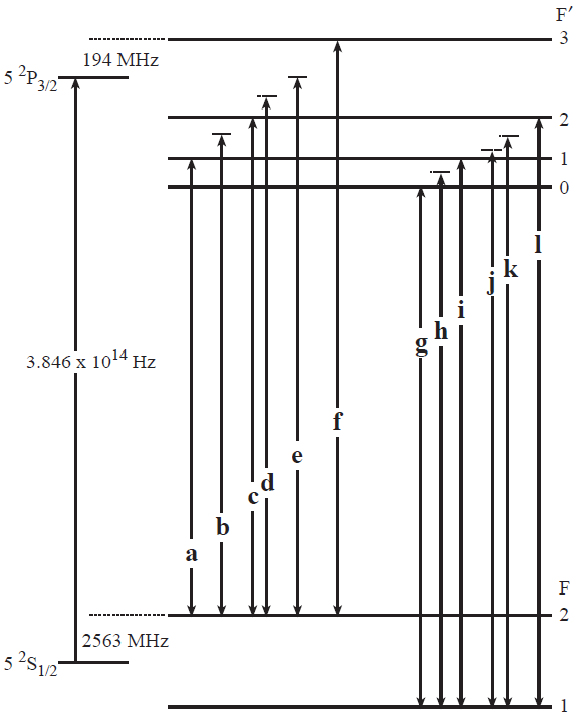
\includegraphics{Figures/4/Crossover.png}
    \caption{Transition frequencies with croosover frequencies for the $D_2$ and $D_1$ line of $^{87}$Rb. \cite{nakayama_1984_theoretical}}
    \label{fig:crossover_frequencies}
\end{figure}

If the laser frequency is positioned midway between two atomic resonances, atoms with a specific velocity are precisely resonant with both the pump and probe beams.
However, the contra-propagating beams resonate with different atomic transitions, defining this frequency as the Crossover frequency. Using [\ref{app:frequencies}], these crossover frequencies were calculated in [\ref{app:crossover_frequencies}].

\pagebreak{}

So, the following table shows the comparison between the experimental and theoretical crossover frequencies found in [\ref{fig:lamb_dips}]

\begin{table}[h]
    \centering
    \begin{tabular}{|ccc|ccc|}
    \hline
    \multicolumn{3}{|c|}{\textbf{Peak 1, $^{87}\text{Rb}_1$}} &
      \multicolumn{3}{c|}{\textbf{Peak 2, $^{85}\text{Rb}_2$}} \\ \hline
    \multicolumn{1}{|c|}{Experimental} &
      \multicolumn{1}{c|}{Theoretical} &
      \% Error &
      \multicolumn{1}{c|}{Experimental} &
      \multicolumn{1}{c|}{Theoretical} &
      \% Error \\ \hline
    \multicolumn{1}{|c|}{78.8} &
      \multicolumn{1}{c|}{78.5 ($C_{12}$)} &
      0.38 &
      \multicolumn{1}{c|}{64.3} &
      \multicolumn{1}{c|}{63.4 ($F_{23}$)} &
      1.42 \\ \hline
    \multicolumn{1}{|c|}{193.1} &
      \multicolumn{1}{c|}{211.8 ($C_{13}$)} &
      8.83 &
      \multicolumn{3}{c|}{} \\ \hline
    \multicolumn{3}{|c|}{\textbf{Peak 3, $^{85}\text{Rb}_3$}} &
      \multicolumn{3}{c|}{\textbf{Peak 4, $^{87}\text{Rb}_2$}} \\ \hline
    \multicolumn{1}{|c|}{Experimental} &
      \multicolumn{1}{c|}{Theoretical} &
      \% Error &
      \multicolumn{1}{c|}{Experimental} &
      \multicolumn{1}{c|}{Theoretical} &
      \% Error \\ \hline
    \multicolumn{1}{|c|}{115.8} &
      \multicolumn{1}{c|}{120.6 ($F_{34}$)} &
      3.98 &
      \multicolumn{1}{c|}{113.1} &
      \multicolumn{1}{c|}{114.6 ($C_{02}$)} &
      1.31 \\ \hline
    \multicolumn{1}{|c|}{60.1} &
      \multicolumn{1}{c|}{60.3 ($C_{34}$)} &
      0.33 &
      \multicolumn{1}{c|}{192.9} &
      \multicolumn{1}{c|}{211.8 ($C_{13}$)} &
      8.92 \\ \hline
    \end{tabular}
    \caption{Comparison between experimental and theoretical crossover frequencies. $C_{ij}$ and $F_{ij}$ denote the crossover frequencies between the $i$th and $j$th hyperfine states of the excited and ground states, respectively.}
\end{table}

\pagebreak{}

\section{Conclusion}

In this experiment, we successfully scaled the data using the FPI peaks and determined the finesse. We then analyzed the effect of changing the temperature and injection current of the diode on the saturation spectra. We observed that changing the current had a more significant effect on the spectrum than changing the temperature. This could be due to the fact that a slight change in the current leads to more heating compared to the temperature increments we used. 
In task 3 we observed the effect of changing the filter orientation on the saturation spectra. We found that the peak heights changed with a change in filter angle, with a jump at 180 degrees. We also observed that changing the filter thickness only affected the intensity of the dips.
In task 4, we found the absorption spectrum peaks and compared the distances between them to the theoretical values. We also fitted the peaks with a Voigt profile and compared the FWHM values to the theoretical value. We found that the \% errors were high for most peaks, probably due to the fitting algorithm. We also found the lamb dips and compared the experimental crossover frequencies to the theoretical values. The \% errors were within 10\% for most peaks, with the highest error being 8.92\%.

\pagebreak{}

\begin{appendices}

\section{Frequencies}
\label{app:frequencies}

\begin{figure}[h]
    \centering
    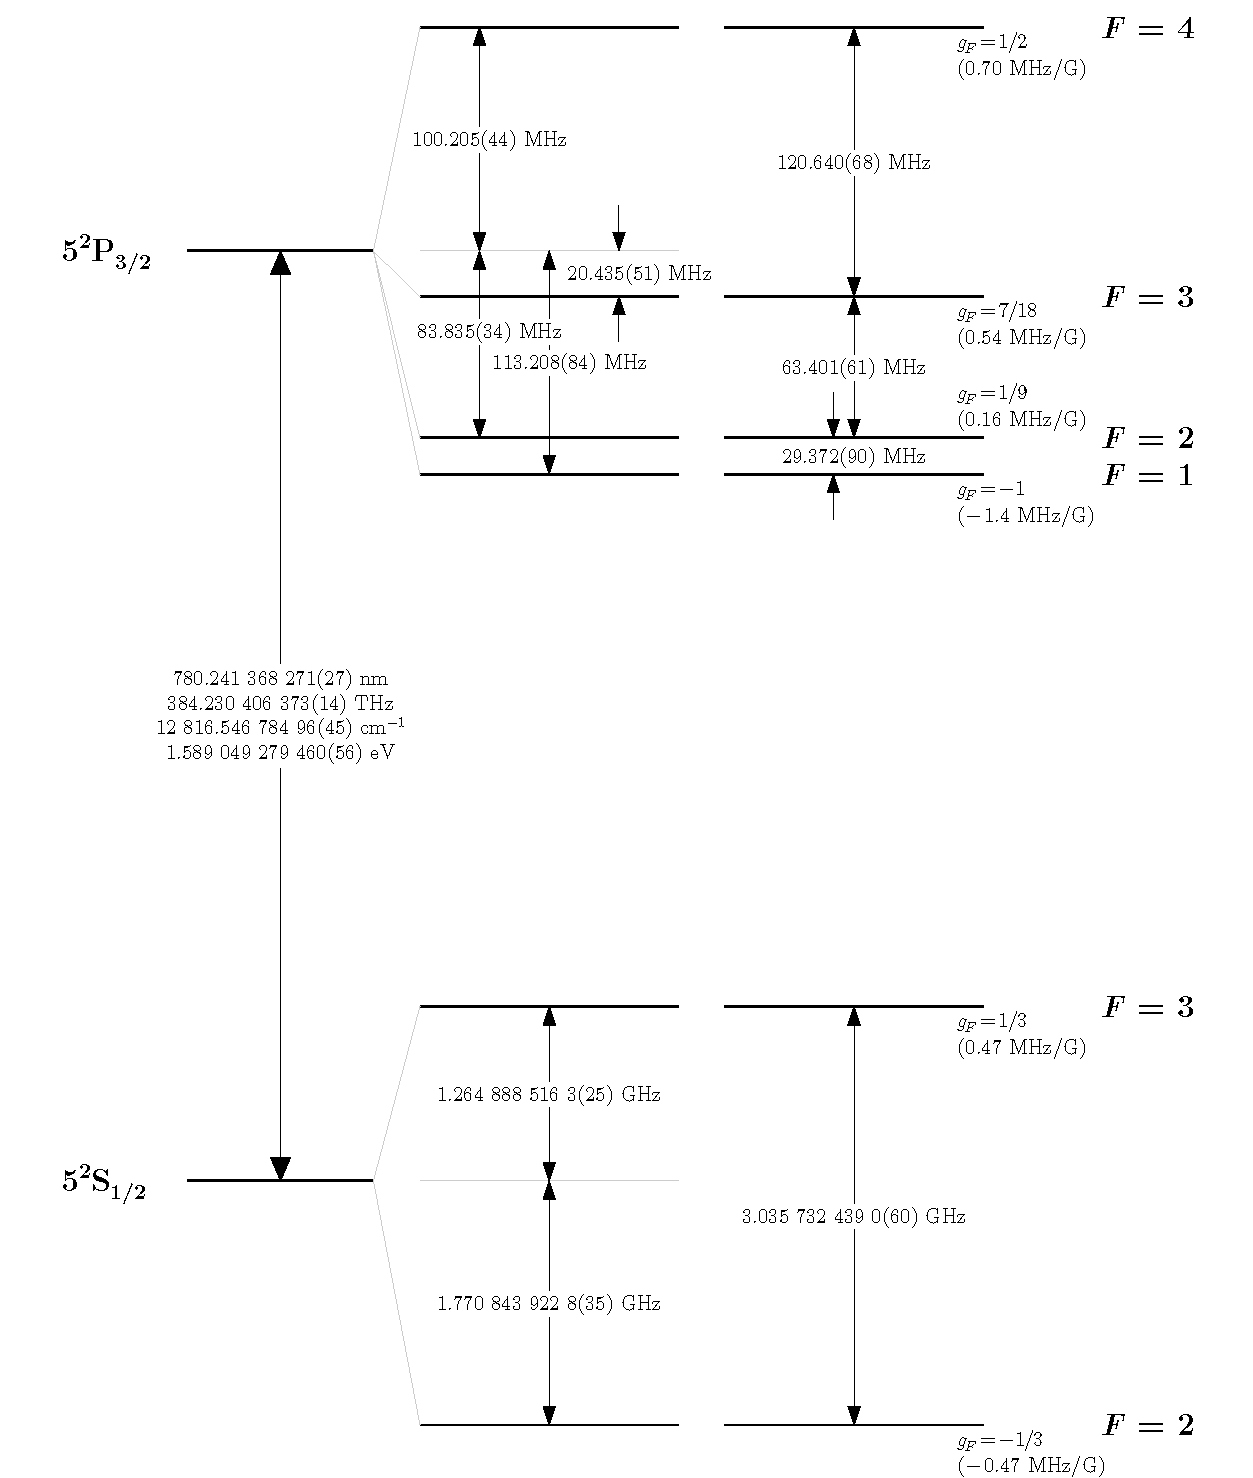
\includegraphics{Figures/4/rubidium85numbers.png}
    \caption{Transition frequencies for $^{85}$Rb. \cite{asteck_alkali}}
    \label{fig:transition_frequencies_Rb85}
\end{figure}

\pagebreak{}

\begin{figure}[h]
    \centering
    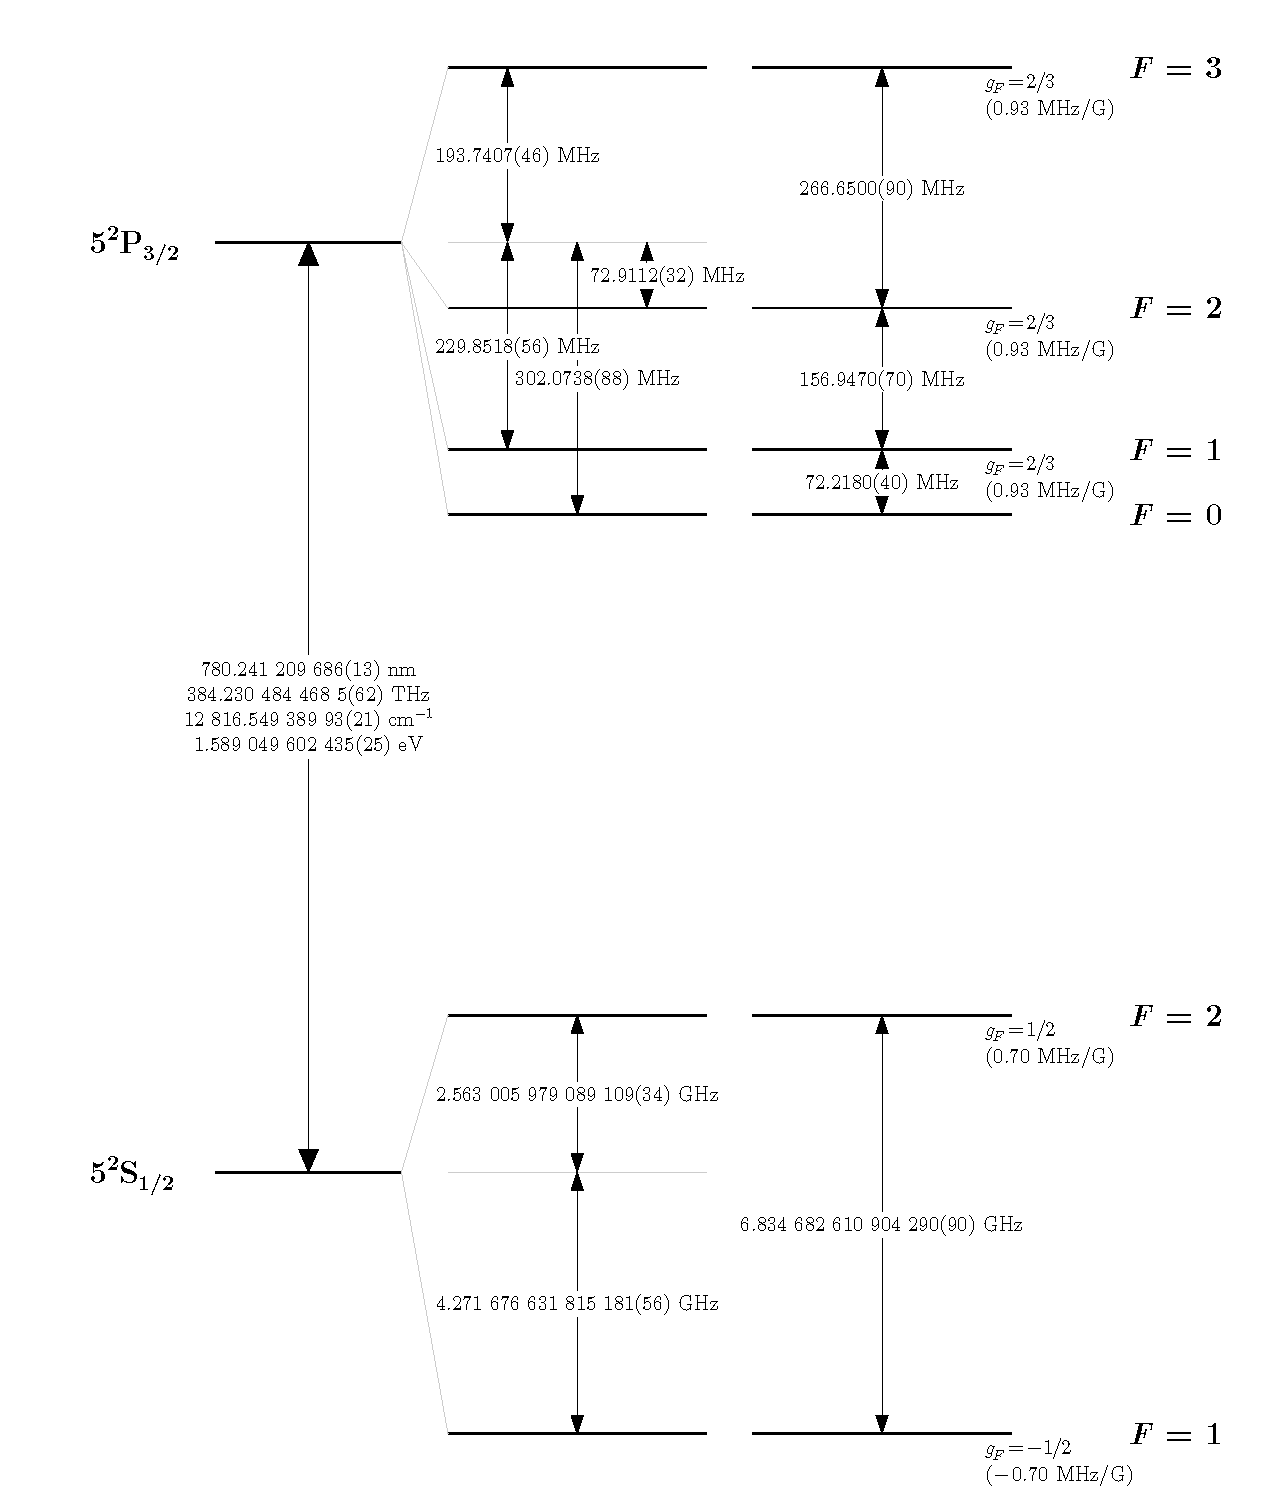
\includegraphics{Figures/4/rubidium87numbers.png}
    \caption{Transition frequencies for $^{87}$Rb. \cite{asteck_alkali}}
    \label{fig:transition_frequencies_Rb87}
\end{figure}

\pagebreak{}

\section{Crossover Frequencies
\label{app:crossover_frequencies}}

\begin{table}[h]
    \centering
    \begin{tabular}{|l|l|l|l|}
    \hline
    $^{85}$Rb & $F = 1$ & $F = 2$ & $F = 3$ \\ \hline
    $F' = 2$  & 14.686  &         &         \\ \hline
    $F' = 3$  & 46.500  & 31.700  &         \\ \hline
    $F' = 4$  & 106.707 & 92.021  & 60.320  \\ \hline
    \end{tabular}
    \label{tab:crossover_frequencies_Rb85}
\end{table}

\begin{table}[]
    \centering
    \begin{tabular}{|l|l|l|l|}
    \hline
    $^{87}$Rb & $F = 0$ & $F = 1$ & $F = 2$ \\ \hline
    $F' = 1$  & 36.109  &         &         \\ \hline
    $F' = 2$  & 114.583 & 78.474  &         \\ \hline
    $F' = 3$  & 247.908 & 211.799 & 133.325 \\ \hline
    \end{tabular}
    \label{tab:crossover_frequencies_Rb87}
\end{table}



\end{appendices}

\pagebreak{}

\bibliographystyle{ieeetr} 
\bibliography{rbspectroscopy} 

\end{document}